\documentclass[10pt]{report}
\usepackage[utf8]{inputenc}
\usepackage[letterpaper, margin=1in]{geometry}
\usepackage[spanish, es-tabla]{babel}
\usepackage{graphicx}
\usepackage{setspace}
\usepackage{verbatim}
\usepackage[dvipsnames]{xcolor}
\usepackage{amsmath,bm,amsthm, amsfonts,amssymb}
\usepackage{mathtools,cancel}
\usepackage{multicol}
\usepackage{listings}
\lstset{basicstyle=\footnotesize\ttfamily,breaklines=true}
\usepackage{alltt}
\usepackage{gensymb}
\usepackage{subfigure} 
\usepackage{ragged2e}
\usepackage{minted}
\usemintedstyle{tango}
\usepackage{pifont}
\usepackage{hyperref}
\usepackage{url}
\usepackage{float}
\usepackage{tcolorbox}
\tcbuselibrary{listings}
\tcbuselibrary{minted}

% tensor 2:
\newcommand{\tend}[1]{\hbox{\oalign{$\bm{#1}$\crcr\hidewidth$\scriptscriptstyle\bm{\sim}$\hidewidth}}}

%tensor 4:
\newcommand{\tenq}[1]{\hbox{\oalign{$\bm{#1}$\crcr\hidewidth$\scriptscriptstyle\bm{\approx}$\hidewidth}}}

\newcommand{\cmark}{\ding{51}}
\newcommand{\xmark}{\ding{55}}

\graphicspath{{Figuras/}}

\hypersetup{
    colorlinks=true,
    linkcolor=blue,
    filecolor=magenta,      
    urlcolor=cyan,
    pdftitle={Dinamica Estructural Avanzada},
    pdfauthor={Gaston Fermandois},
    pdfpagemode=UseOutlines,
    }

\setminted{
    autogobble=true,
    breaklines=true,
    linenos=false,
    fontsize=\footnotesize
}

% Definir el nuevo entorno verbatimg
\newtcblisting{verbatimg}{
    colback=lightgray,
    listing only,
    left=0pt,
    listing options={
        style=Matlab,
        showstringspaces=false % Espacios normales
    },
    minted options={
        fontsize=\normalsize
    }
}

\def\version{2.0}

\begin{document}

\begin{titlepage}
    \centering

    \vspace*{1cm}

    % Title and subtitle are enclosed between two rules.
    \rule{\textwidth}{1pt}

    % Title
    \vspace{.7\baselineskip}
    {\huge \textbf{MIC411 Dinámica Estructural Avanzada}}

    % Subtitle
    \vspace*{.5cm}
    {\LARGE Apuntes de Clases}
    
    \rule{\textwidth}{1pt}

    \vspace{1cm}

    % Set this size for the remaining titlepage.
    \large

    % Authors side by side, using two minipages as a trick.
    \begin{minipage}{.6\textwidth}
        \centering
        Gastón Fermandois Cornejo, Ph.D, Ing. \\
        Departamento de Obras Civiles \\
        Universidad Técnica Federico Santa María\\
        Valparaíso, Chile \\
        {\normalsize \url{gaston.fermandois@usm.cl}}
    \end{minipage}%

    % More authors can be inserted here with additional minipages.

    \vspace{2cm}

    % Report logo.
    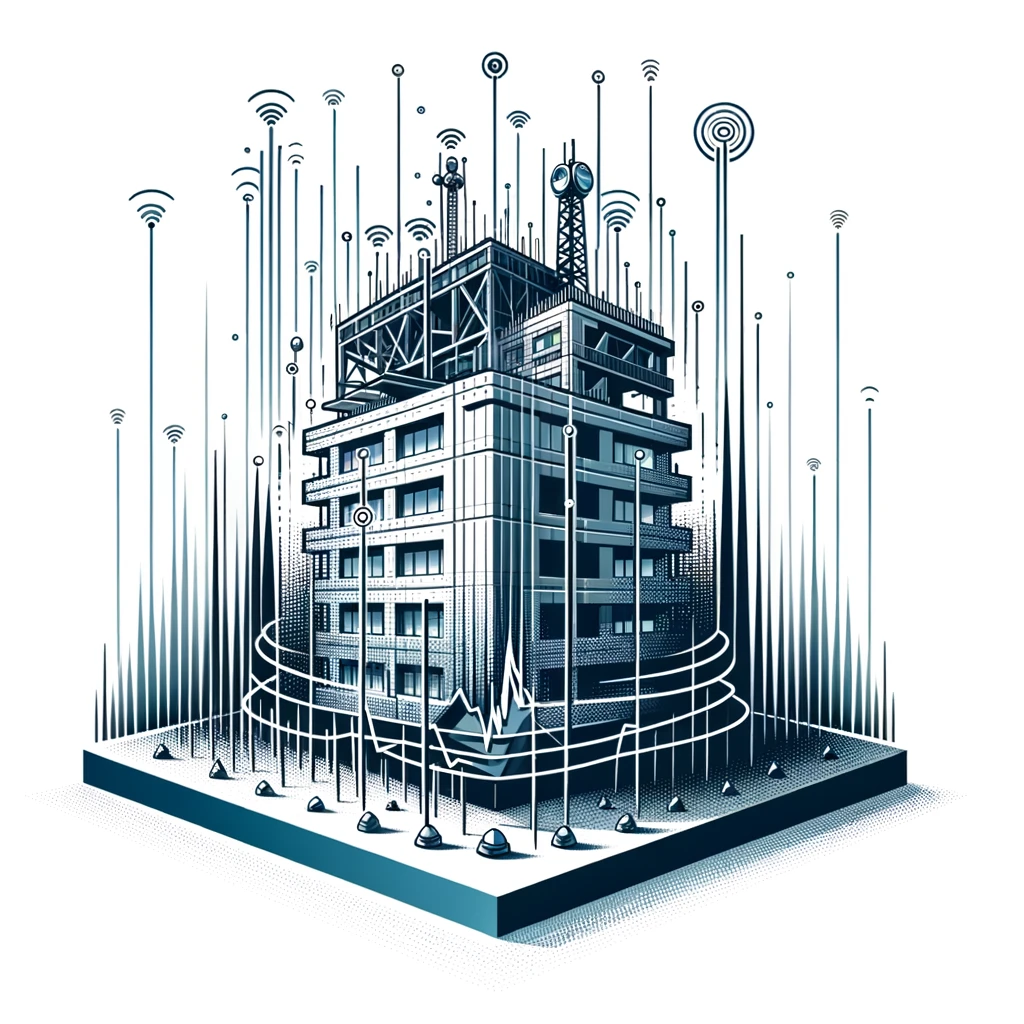
\includegraphics[width=.7\textwidth]{logoSHM.png}

    \vfill

    % University and date information at the bottom of the titlepage.
    Versión \version\ (\today)
    
\end{titlepage}

\pagenumbering{Roman}

\chapter*{Prefacio}

Este es un curso avanzado sobre dinámica estructural, que incluye aplicaciones en el modelamiento de sistemas dinámicos sometidos a cargas estocásticas, sistemas de monitoreo y control estructural, problemas inversos o de identificación de sistemas, entre otros. Los conceptos y las técnicas cubiertas en este curso son fundamentales para realizar investigación aplicada y desarrollo tecnológico en el campo de la ingeniería estructural, con énfasis en el diseño de sistemas estructurales inteligentes (\emph{smart structures}).

El apunte se divide en tres grandes partes. La primera parte se enfoca principalmente en establecer las bases de la teoría de sistemas dinámicos lineales contínuos y discretos en el tiempo, sujetos a cargas determinísticas o estocásticas. La segunda parte, se concentra en el desarrollo de aplicaciones avanzadas en dinámica estructural, principalmente lo relacionado con monitoreo y control estructural. Finalmente, la tercera parte esta dedicado a tópicos avanzados que avanzan muy rápidamente junto con el estado del arte en dinámica estructural. Temas como simulación híbrida y aprendizaje automático son sólo una selección de tópicos cubiertos en esta última parte.

Agradecimientos a María Elena Quiroz (M.S., Ing. USM), quien fue la segunda ayudante de docencia del curso IPO426 en el primer semestre de 2022. María Elena fue quien tomó mis apuntes tomados a mano en las primeras instancias del curso, y las transcribió en este documento. Además, fue ella la que preparó la totalidad de figuras e ilustraciones del primer borrador de este apunte de clases. También agradezco a Alexis Contreras (Ing. y estudiante magíster USM), el tercer ayudante de docencia del curso IPO426/MIC411 realizado el primer semestre de 2024. En particular, Alexis ayudó a revisar todo el contenido de estos apuntes, y también colaboró en la elaboración de nuevos capítulos, como por ejemplo el de sensores. Por último, agradecimientos especiales a Cristobal Gálmez (M.S., Ing. USM), el primer ayudante de docencia del curso IPO426 realizado el primer semestre de 2020.

\bigskip\noindent
\begin{flushright}
  Gastón Fermandois\\
  5 de agosto de 2025\\
  Valparaíso, Chile
\end{flushright}

\chapter*{Versiones}

\section*{Versión 4}
\subsection*{1 Diciembre 2025}

\begin{itemize}
    \item Se funden capítulos en dos nuevas partes: Parte 2 "Monitoreo Estructual" y Parte 3 "Control Estructural".
    \item Varias revisiones menores de edición en todo el documento.
\end{itemize}

\section*{Versión 3}
\subsection*{26 Agosto 2025}

\begin{itemize}
    \item Grandes cambios en Parte 1, se agregan capítulos de modelos lineales y análisis de sistemas lineales. 
    \item En Parte 2 se agrega un capítulo (placeholder) de modelos nolineales, para completar en un futuro.
    \item Agrega capítulo de sistemas nolineales.
    \item Agrega referencias bibliográficas.
    \item Completa el Apendice B de Simulink.
    \item Varias revisiones mayores de edición en todo el documento.
\end{itemize}

\section*{Versión 2}
\subsection*{6 Agosto 2025}

\begin{itemize}
    \item Varias revisiones mayores de edición en todo el documento.
\end{itemize}

\section*{Versión 1}
\subsection*{18 julio 2024}

\begin{itemize}
    \item Capítulo de procesamiento digital de señales pasa a la Parte 1 del apunte.
    \item Sección de especificaciones transientes de sistemas lineales pasa al capítulo de Control Clásico.
    \item Sección de observadores y principio de separación pasa al capítulo de Control Clásico.
    \item Varias revisiones de edición.
\end{itemize}

\section*{Versión 0}
\subsection*{12 marzo 2024}

\begin{itemize}
    \item Primer borrador del apunte de clases.
\end{itemize}

\pdfbookmark{\contentsname}{toc}
\tableofcontents

\newpage

\pagenumbering{arabic}

\part{Teoría}

\chapter{Sistemas dinámicos}

\section{Generalidades}

En ingeniería estructural, un sistema se refiere al conjunto de elementos estructurales interconectados que trabajan en conjunto para resistir cargas y garantizar la estabilidad y seguridad de una construcción. En particular, un sistema dinámico es una estructura cuya respuesta varía en el tiempo ante cargas cambiantes, como sismos, viento, impactos o transito.

Al estudiar sistemas dinámicos es fundamental distinguir entre el sistema físico y el modelo matemático. El sistema físico es la estructura real, con sus materiales, geometría y condiciones de carga, sujeta a imperfecciones y a interacciones complejas con el entorno. En cambio, el modelo matemático es una representación simplificada que traduce ese comportamiento en ecuaciones, permitiendo predecir su respuesta bajo distintas condiciones.

Estos modelos matemáticos se construyen a partir de principios fundamentales, es decir, de las leyes físicas que gobiernan la mecánica estructural. Entre ellas destacan la cinemática y compatibilidad geométrica, ecuaciones de balance (Newton, Lagrange, etc.), relaciones constitutivas de los materiales, y la geometería y condiciones de contorno e iniciales del sistema físico. A partir de estos principios, se generan modelos matemáticas que representan de forma coherente el comportamiento de la estructura, aunque siempre con ciertas simplificaciones necesarias para el análisis.

Los sistemas sistemas dinámicos pueden ser representados gráficamente por diagramas de bloques:

\begin{figure}[H]
    \centering
    
\includegraphics[scale=0.7]{sistema.png}
    \caption{Representación de un sistema dinámico}
\end{figure}

Principales razones para construir modelos matemáticos de sistemas dinámicos:

\begin{enumerate}
    \item Análisis
    \item Diseño
    \item Control y monitoreo
\end{enumerate}

\section{Tipos de sistemas}

\subsection{Estáticos vs Dinámicos}

\begin{itemize}
    \item Sistema Estático: respuesta solo depende de la excitación actual (independiente del tiempo).
    \begin{figure}[H]
    \centering
    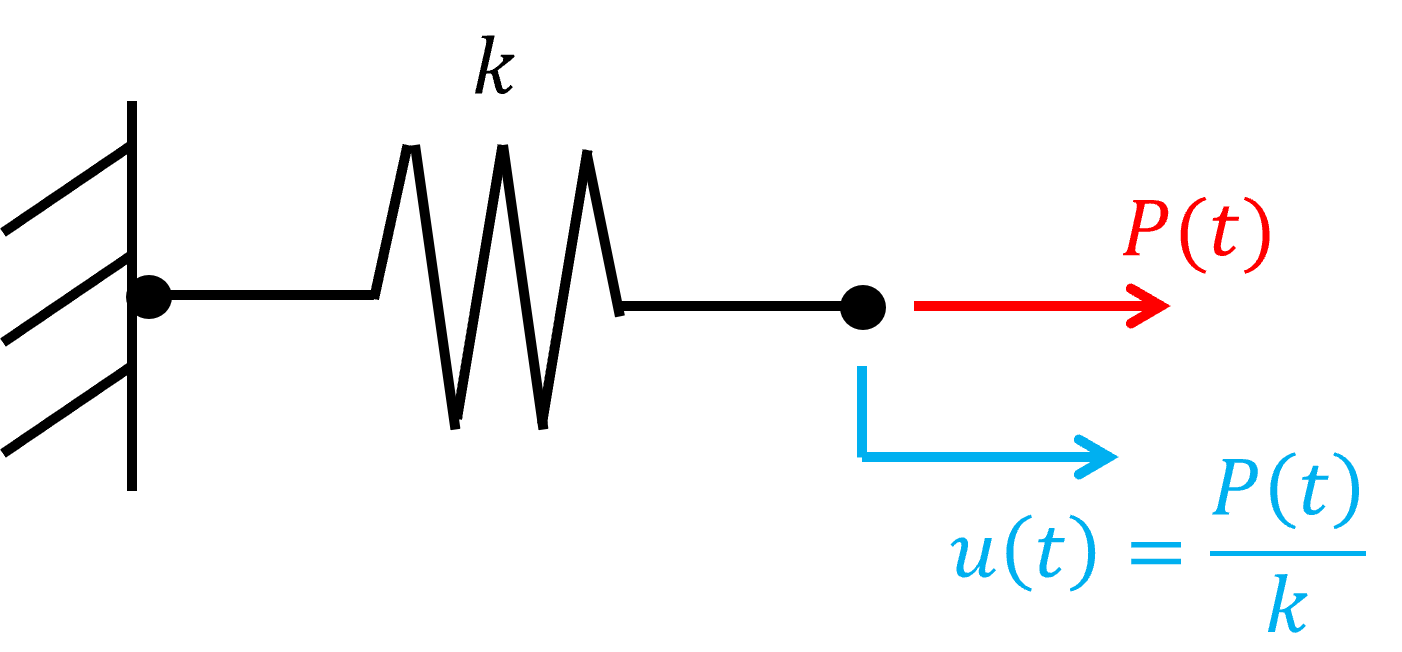
\includegraphics[scale=0.7]{estatico.png}
    \end{figure}
    
    \item Sistema Dinámico: respuesta actual depende de la excitación actual y de la ``historia'' de la respuesta.
    \begin{figure}[H]
    \centering
    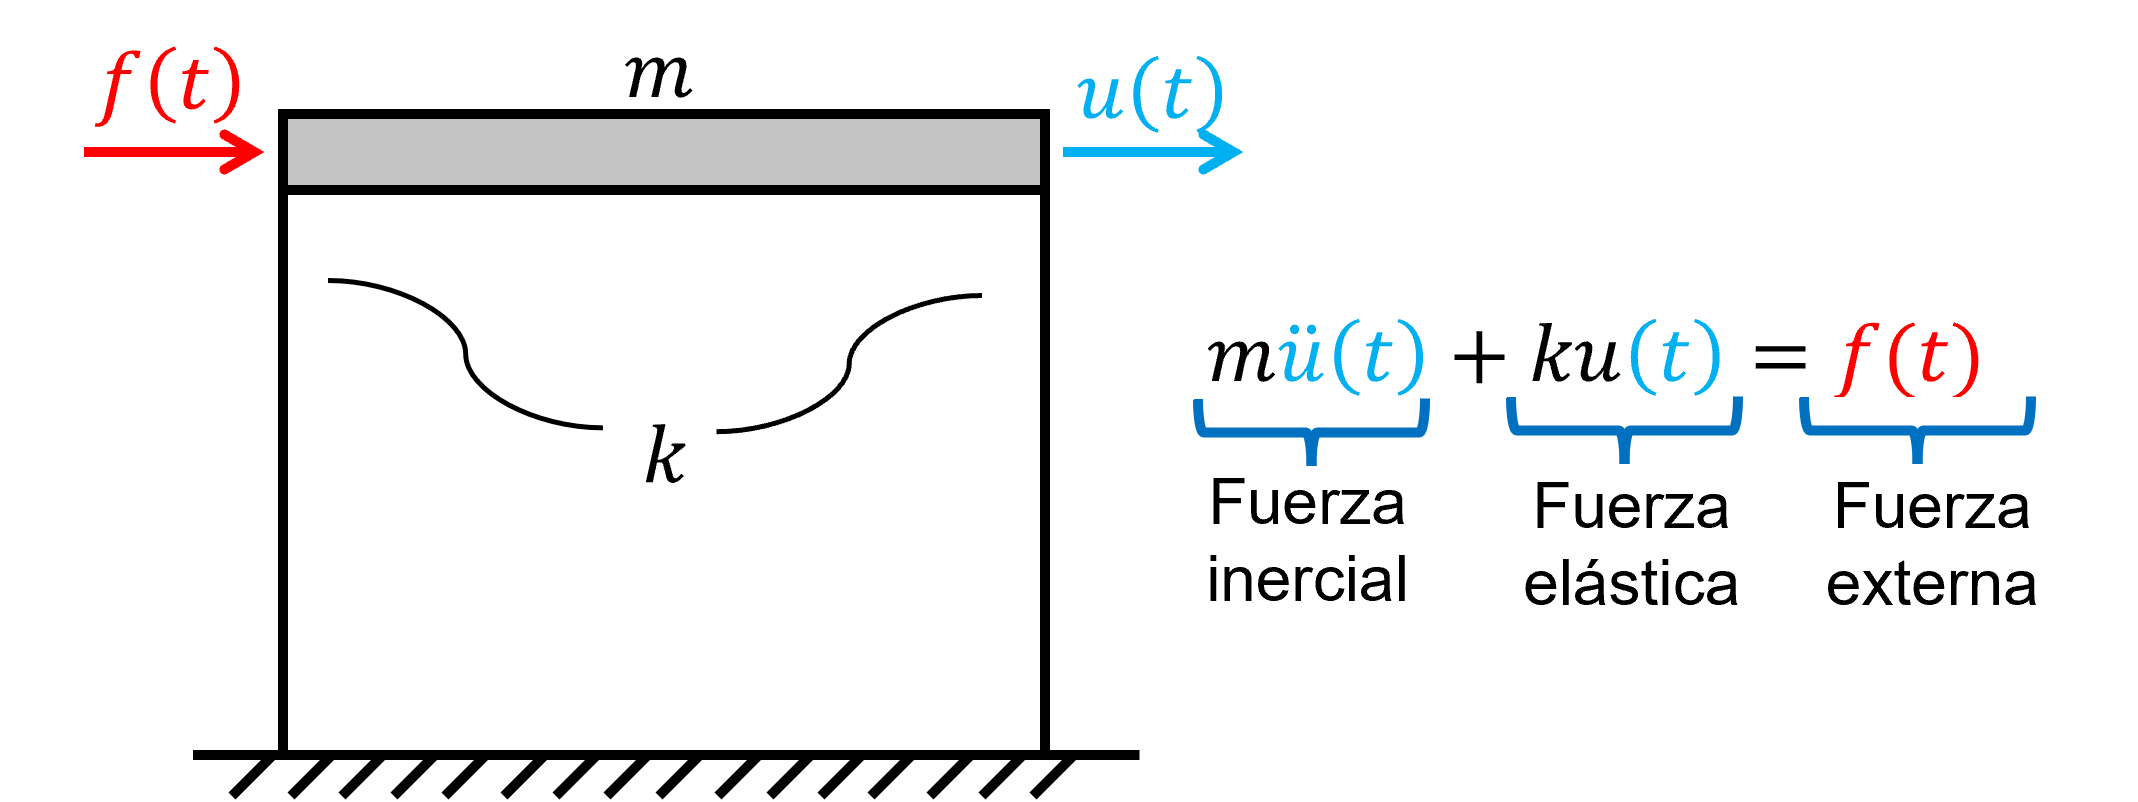
\includegraphics[scale=0.7]{dinamico.png}
    \end{figure}
    \par Si la respuesta del sistema dinámico está basada en la excitación actual y pasada, entonces el sistema se conoce como \textcolor{red}{causal} (todos los sistemas físicos).\\
    \par Si la respuesta del sistema dinámico está basada en excitación actual, pasada y \textcolor{ForestGreen}{futura}, entonces el sistema es \textcolor{red}{anticausal} (solo aplicable en sistemas teóricos \emph{offline}, por ejemplo, en procesamiento digital de señales).
\end{itemize}

\subsection{Univariado vs Multivariado}
\begin{itemize}
    \item SISO: Single Input, Single Output.
    \begin{figure}[H]
    \centering
    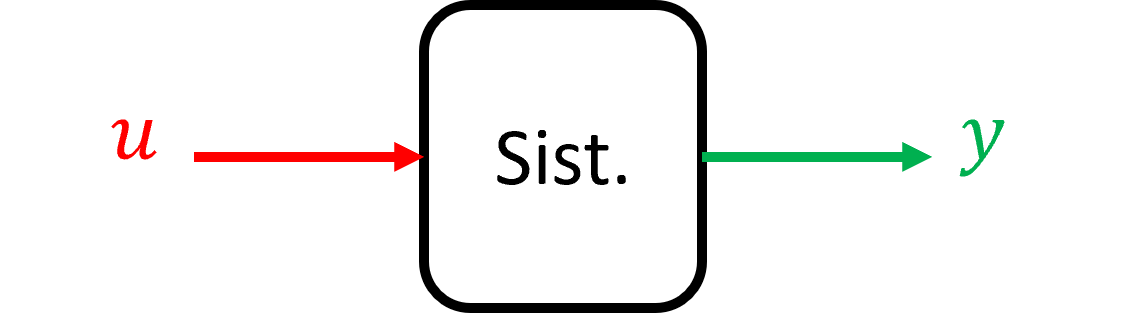
\includegraphics[scale=0.7]{SISO.png}
    \end{figure}
    \begin{itemize}
        \item $u \in \mathbb{R}$: entrada escalar
        \item $y \in \mathbb{R}$: respuesta escalar
        % \item $f(u)=y$: función escalar
    \end{itemize}
    
    \item SIMO: Single Input, Multi Output.
    \begin{figure}[H]
    \centering
    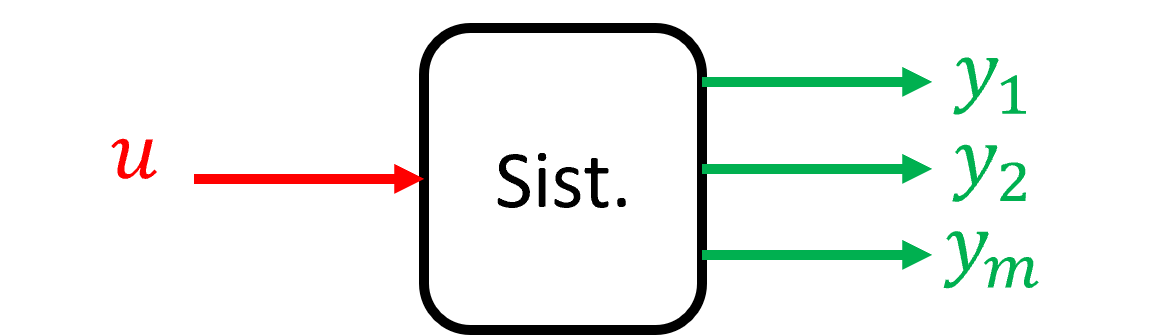
\includegraphics[scale=0.7]{SIMO.png}
    \end{figure}
    \begin{itemize}
        \item $u \in \mathbb{R}$: entrada escalar
        \item $y \in \mathbb{R}^m$: respuesta vectorial
    \end{itemize}
    
    \item MISO: Multi Input, Simple Output.
    \begin{figure}[h]
    \centering
    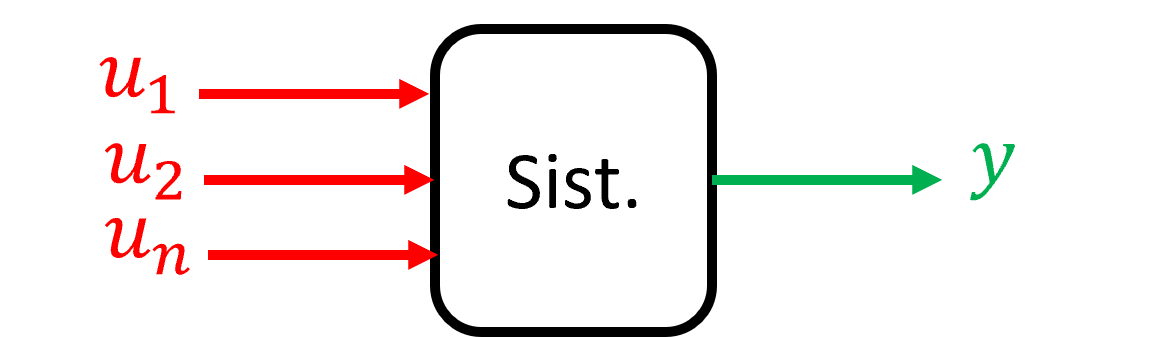
\includegraphics[scale=0.7]{MISO.png}
    \end{figure}
    \begin{itemize}
        \item $u \in \mathbb{R}^n$: entrada vectorial
        \item $y \in \mathbb{R}$: respuesta escalar
    \end{itemize}
    
    \item MIMO: Multi Input, Multi Output.
    \begin{figure}[H]
    \centering
    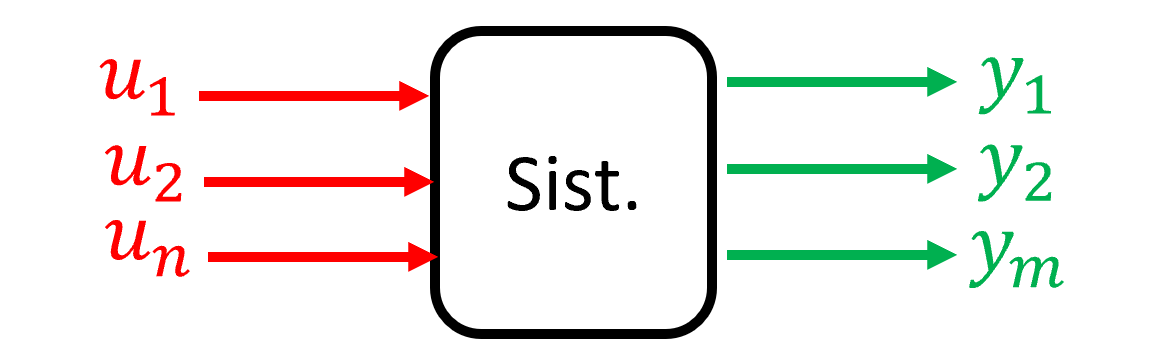
\includegraphics[scale=0.7]{MIMO.png}
    \end{figure}
    \begin{itemize}
        \item $u \in \mathbb{R}^n$: entrada vectorial
        \item $y \in \mathbb{R}^m$: respuesta vectorial
    \end{itemize}
\end{itemize}

\subsection{Lineal vs Nolineal}

\begin{itemize}
    \item Un \emph{sistema lineal} es tal que cumple con el \emph{principio de superposición}.
    
    \begin{itemize}
        \item Aditividad: Si $u_1 \rightarrow y_1$, $u_2 \rightarrow y_2$, entonces: $u = u_1 + u_2 \rightarrow y = y_1 + y_2$
        \item Homogeneidad/Proporcionalidad: Si $u \rightarrow y$, entoncecs ${\alpha}u \rightarrow {\alpha}y$.
    \end{itemize}
    \item De no cumplir con las propiedades del sistema lineal, entonces el sistema es \emph{nolineal}.
\end{itemize}

\par \underline{Ejemplo}: resorte nolineal.\\

\begin{figure}[H]
    \centering
    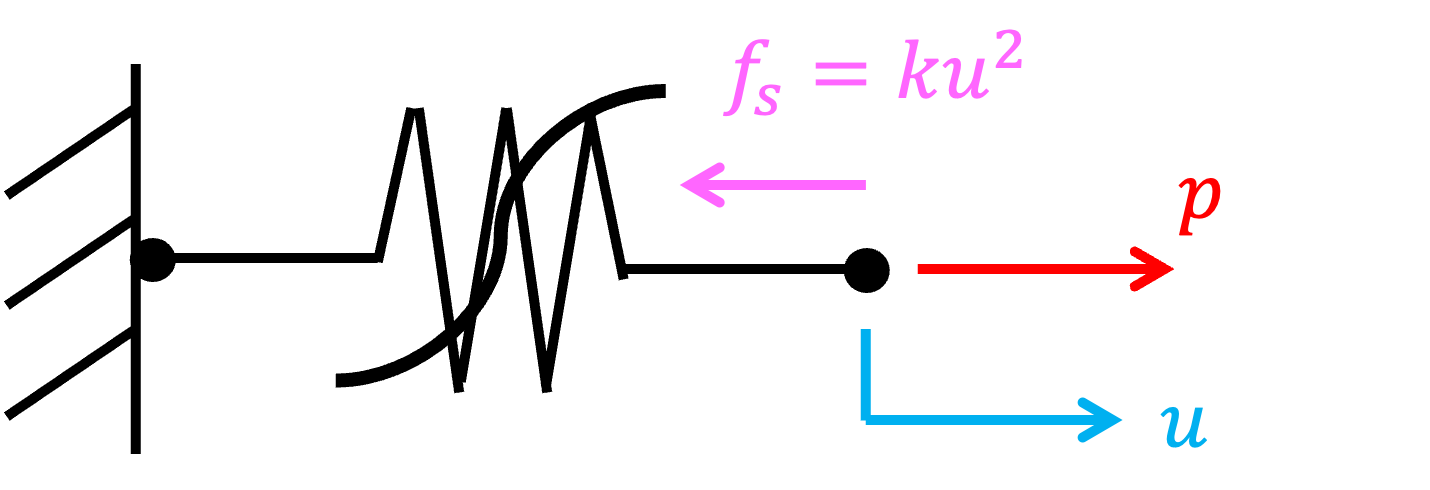
\includegraphics[scale=0.7]{Figuras/resortenolineal.png}
    \caption{Resorte nolineal}
\end{figure}

Se tiene que: 

\begin{align*}
    f_s &= ku^2 \\
    p_1 = k u_1^2 &\rightarrow u_1 = \sqrt{\frac{p_1}{k}}\\  
    p_2 = k u_2^2 &\rightarrow u_2 = \sqrt{\frac{p_2}{k}}\\
\end{align*}

La pregunta es, ¿Se cumple el principio de superposición?

\begin{align*}
    p_1+p_2 &\xrightarrow{?} u_1+u_2
\end{align*}

La respuesta es {no}, ya que:

%\begin{align*}
%    f_s &= k(u_1+u_2)^2 \\
%    p_1 + p_2 & = ku_1^2+ku_2^2+2ku_1u_2\\
%    p_1 + p_2 &\neq p_1 + p_2 + \textcolor{red}{2ku_1u_2}
%\end{align*}

\begin{align*}
    p_1 + p_2 &= k(u_*)^2 \\
    u_* &= \sqrt{\frac{p_1 +p_2}{k}} \neq \sqrt{\frac{p_1}{k}} + \sqrt{\frac{p_2}{k}}
\end{align*}

\subsection{Invariante tiempo vs variante tiempo}

\begin{itemize}

    \item Sistema invariantes en el tiempo (\emph{time invariant}) $\longrightarrow$ parámetros del modelo son constantes en el tiempo.\\
    
    \underline{Ejemplo}: Sistemas de 1GDL (Figura \ref{f:invariante}),  con masa, rigidez y amortiguamiento constante son LTI (\emph{linear time invariant}).
    
    \begin{figure}[h]
        \centering
        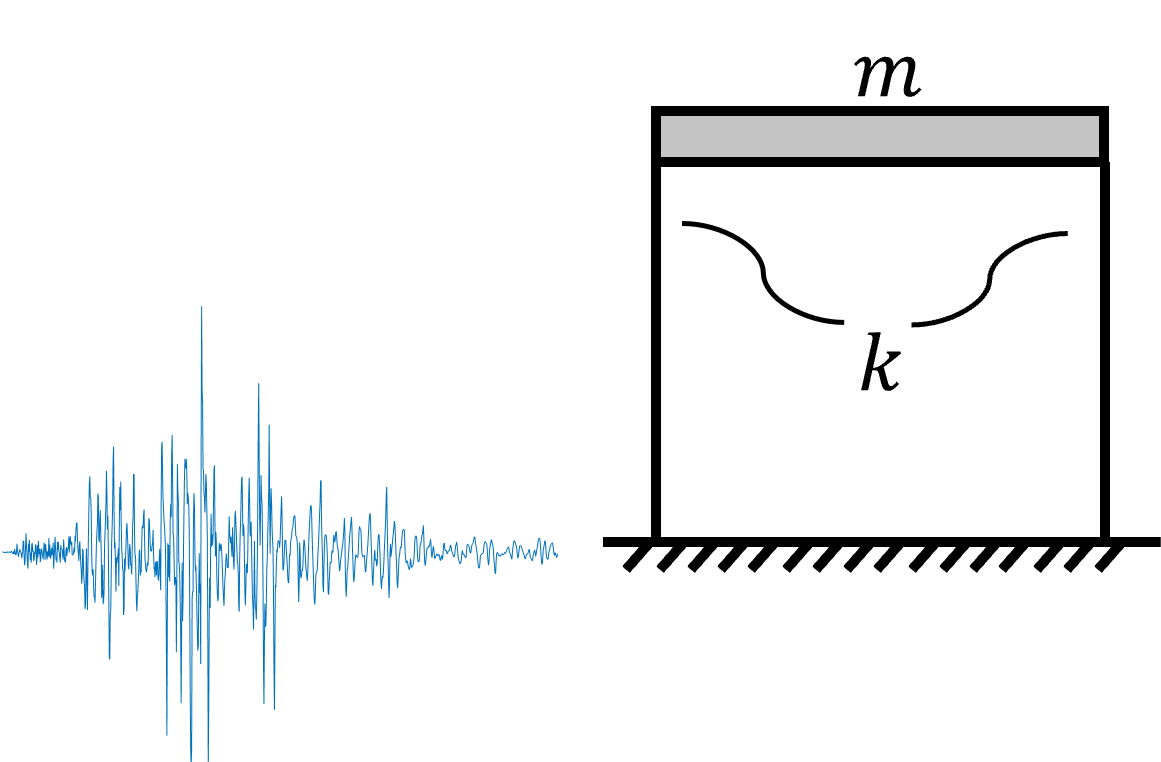
\includegraphics[scale=0.7]{invariante.png}
        \caption{Sistema LTI (\emph{linear time invariant})}
        \label{f:invariante}
    \end{figure}
    
    \item Sistema variante en el tiempo (\emph{time variant}) $\longrightarrow$ parámetros del modelo varían en el tiempo.\\
    
    \underline{Ejemplo}: Puentes con masa movil (Figura \ref{f:movingmass}), por ejemplo por el transito de un vehículo pesado (la masa del sistema varía). En este caso el sistema dinámico es LTV (\emph{linear time variant}).

    \begin{figure}[h]
        \centering
        \includegraphics[width=0.5\textwidth]{movingmass.png}
        \caption{Sistema LTV (\emph{linear time variant})}
        \label{f:movingmass}
    \end{figure}
    
\end{itemize}

\subsection{Determinístico vs Estocástico}

Si el input del sistema es conocido (y el sistema no incorpora incertidumbre), entonces el output será predecible $\longrightarrow$ \textcolor{red}{Determinístico} \\ 

\underline{Ejemplo}: Simular múltiples veces el mismo registro (input) sobre el mismo edifico (sistema), se obtienen siempre las mismas respuestas (output). \\

Si el input del sistema posee incertidumbre (y/o el sistema incorpora incertidumbre), entonces el output también tiene incertidumbre y no es predecible $\longrightarrow$ \textcolor{red}{Estocástico} \\

\underline{Ejemplo}: Simular peatones diferentes (input con incertidumbre en masa del peatón, velocidad al caminar y frecuencia de pasos) sobre un mismo puente (sistema), se obtendrán respuestas diferentes (outputs)\\

% María: Si los parámetros del modelo son conocidos $\longrightarrow$ \textcolor{red}{Determinístico}.\\
% María: Pero, si existe incertidumbre en alguno de los parámetros, o si no se puede predecir de manera precisa la respuesta del sistema $\longrightarrow$ \textcolor{red}{Estocástico}.

\subsection{Continuo vs Discreto}
\begin{itemize}
    \item Sistema Continuo: entrada y salida son función del tiempo.
    \begin{figure}[H]
    \centering
    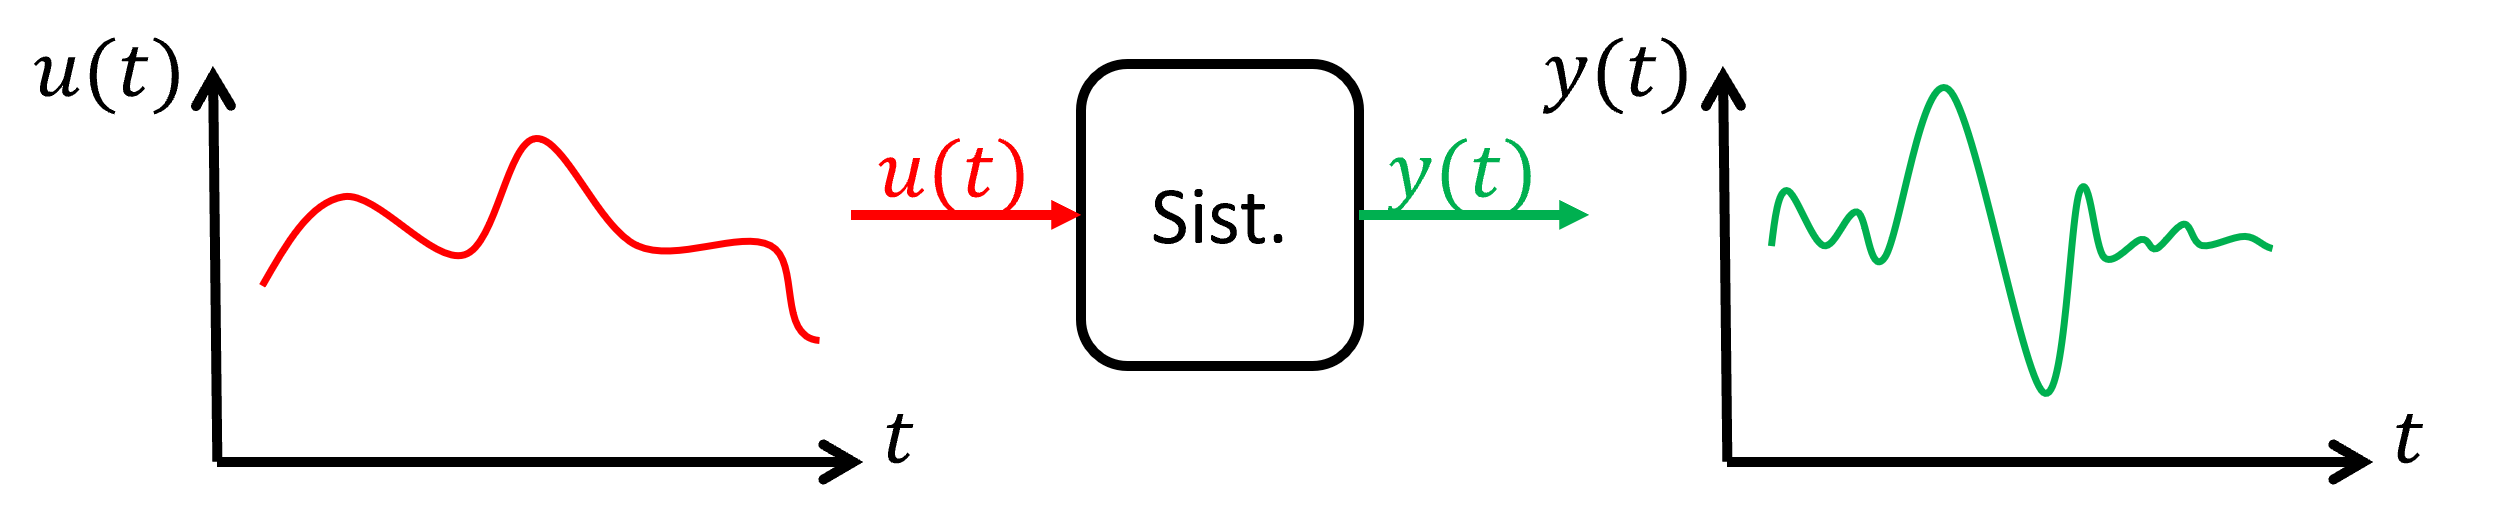
\includegraphics[scale=0.7]{continuo.png}
    \end{figure}
    \item Sistema Discreto: señales han sido discretizadas en el tiempo.\\
    % Ale: Reemplazar el ejemplo por siguiente línea:
    % Ejemplo: Registro de aceleraciones?
    \underline{Ejemplo}: Interés de una cuenta bancaria.
    \begin{align*}
        y(k+1)=(1+r)y(k) \longrightarrow \text{Ecuación de diferencias finitas}
    \end{align*}
    \begin{itemize}
        \item $y(k+1)$: balance cuenta año $k+1$
        \item $r$: interés compuesto anual
        \item $y(k)$: balance cuenta año $k$
    \end{itemize}
\end{itemize}

Las señales de los sistemas físicos son continuas, pero que al momento de ser \emph{observadas} por dispositivos digitales, estas señales se discretizan en función del tiempo.

\begin{figure}[h]
    \centering
    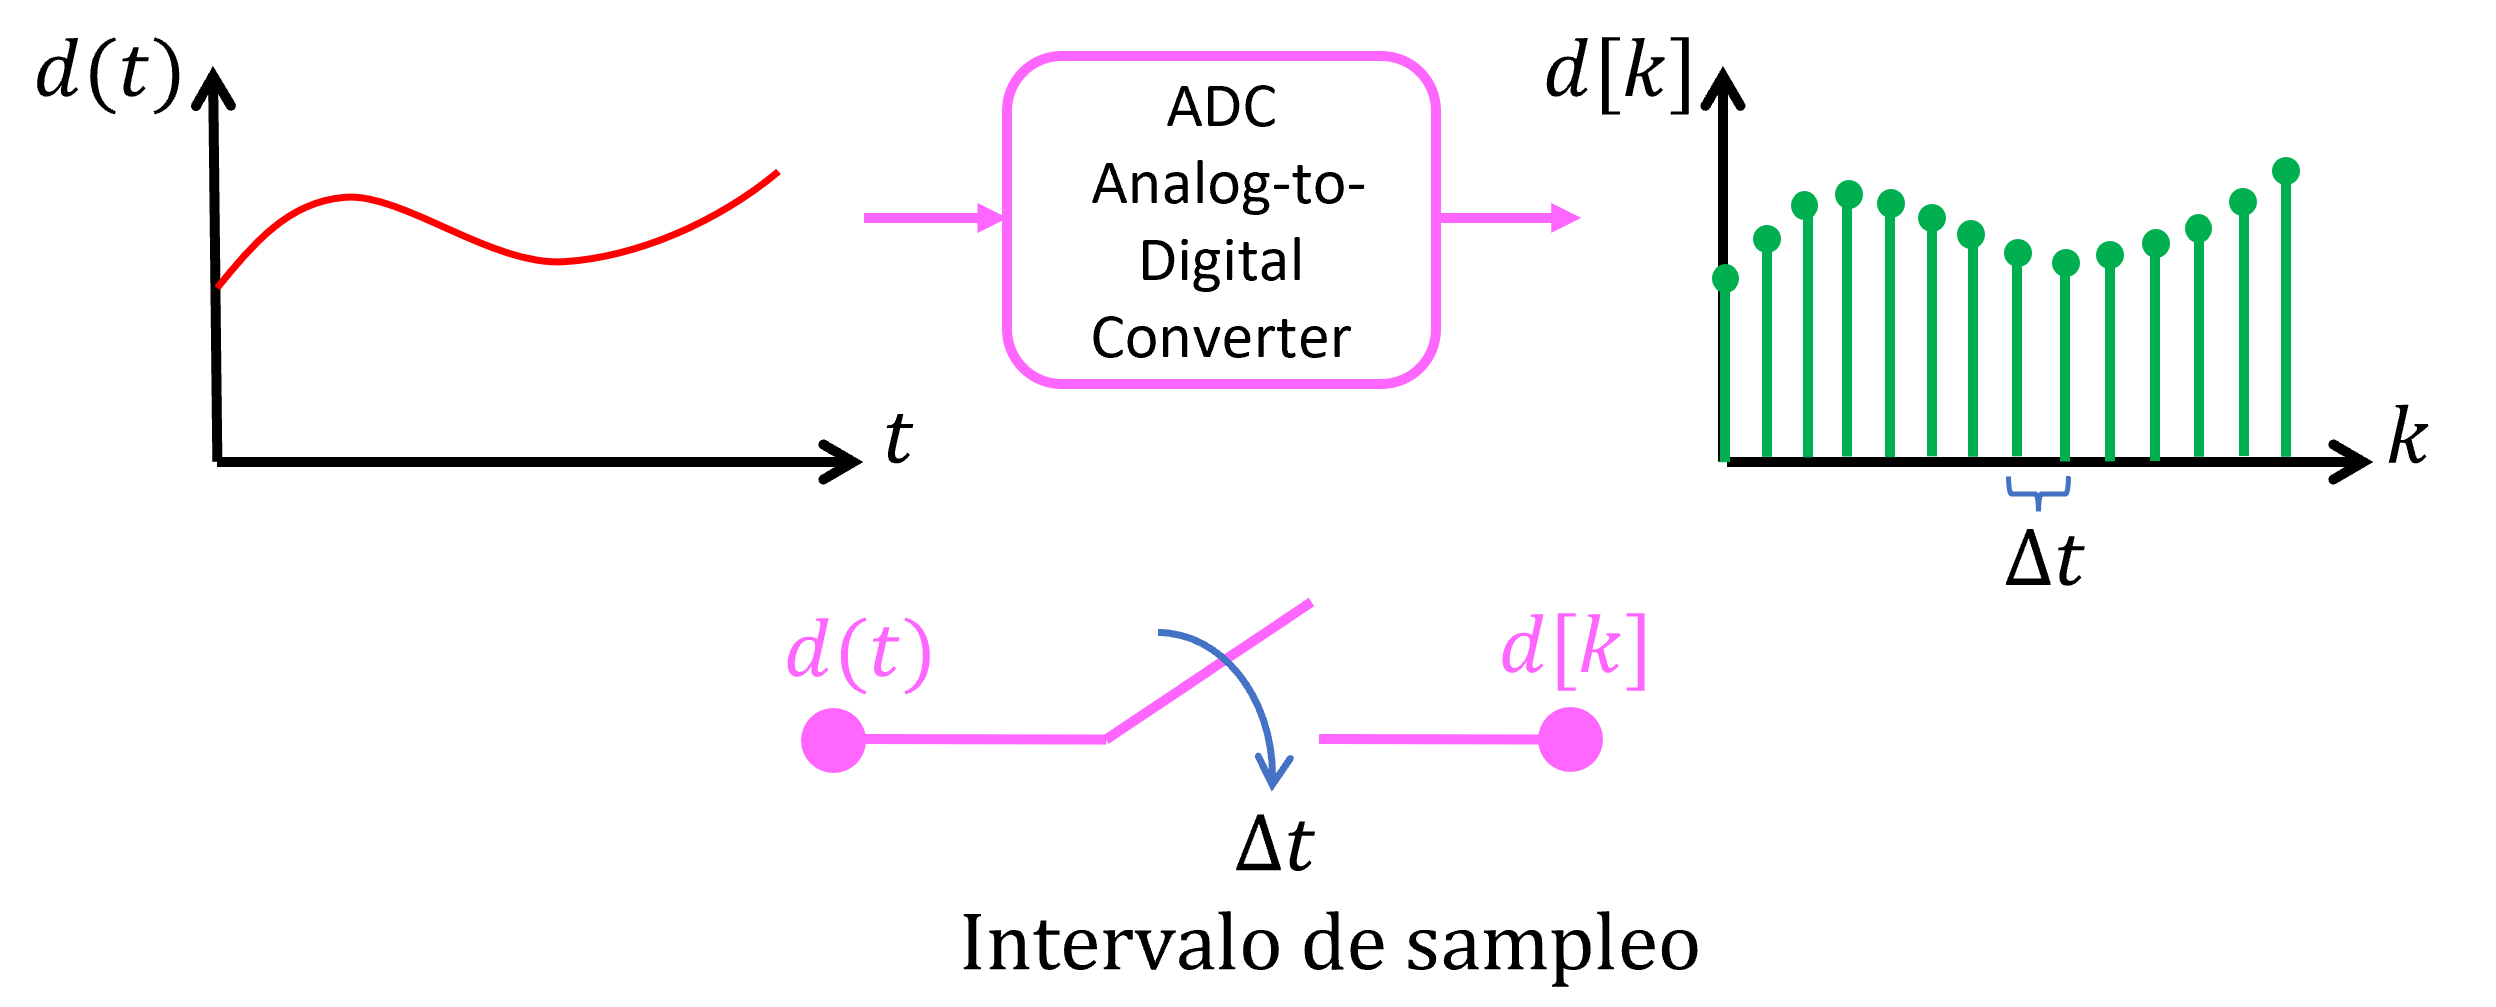
\includegraphics[scale=0.7]{time_sampling.png}
    \end{figure}

\section{Respuesta de sistemas LTI en tiempo continuo}
LTI: Linear, Time-Invariant.

\begin{figure}[H]
    \centering
    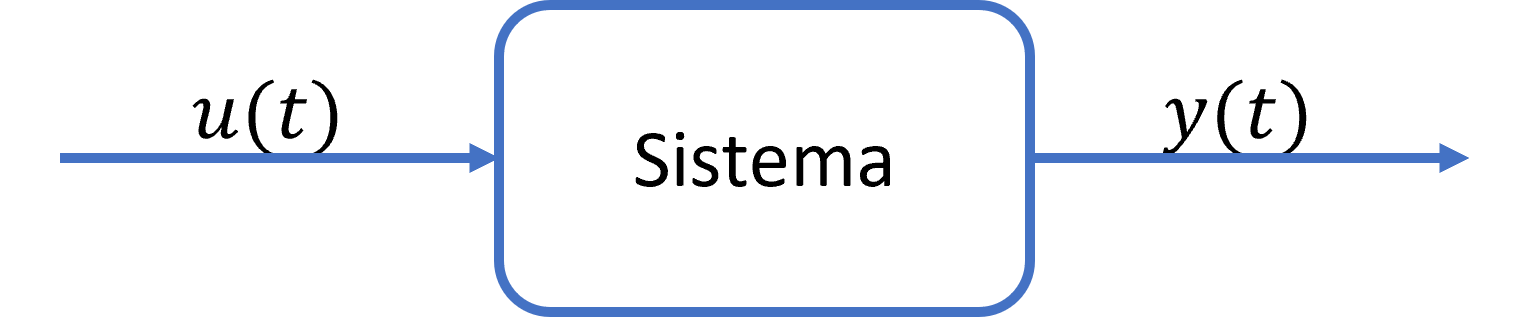
\includegraphics[scale=0.7]{sistemayu.png}
\end{figure}

Los sistemas LTI, son aquellos cuyas propiedades y parámetros no varían en el tiempo, es decir, que los coeficientes de las ecuaciones diferenciales de los modelos matemáticos de los sistemas dinámicos son constantes en el tiempo $a_i=cte$.
\begin{align*}
    \frac{d^ny}{dt^n}+a_{n-1}\frac{d^{n-1}y}{dt^{n-1}}+...+a_2\frac{d^2y}{dt^2}+a_1\frac{dy}{dt}+a_0y=u(t)
\end{align*}
\begin{itemize}
    \item $u(t)$: excitación
    \item $y(t)$: respuesta
    \item $a_i$: coeficientes
\end{itemize}
Dada una excitación $u(t)$, la respuesta se obtiene al resolver la ecuación diferencial:
\begin{align*}
    y(t)=y_H(t)+y_p(t)
\end{align*}
\begin{itemize}
    \item $y_H(t)$ es la \textcolor{red}{respuesta homogénea} (para $u(t)=0$, con condiciones iniciales)
    \item $y_p(t)$ es la \textcolor{red}{respuesta particular} (para $u(t)\neq0$)
\end{itemize}

\section{Modelos de sistemas dinámicos}

Existen diversas formas de modelar un sistema dinámico.

\begin{figure}[H]
    \centering
    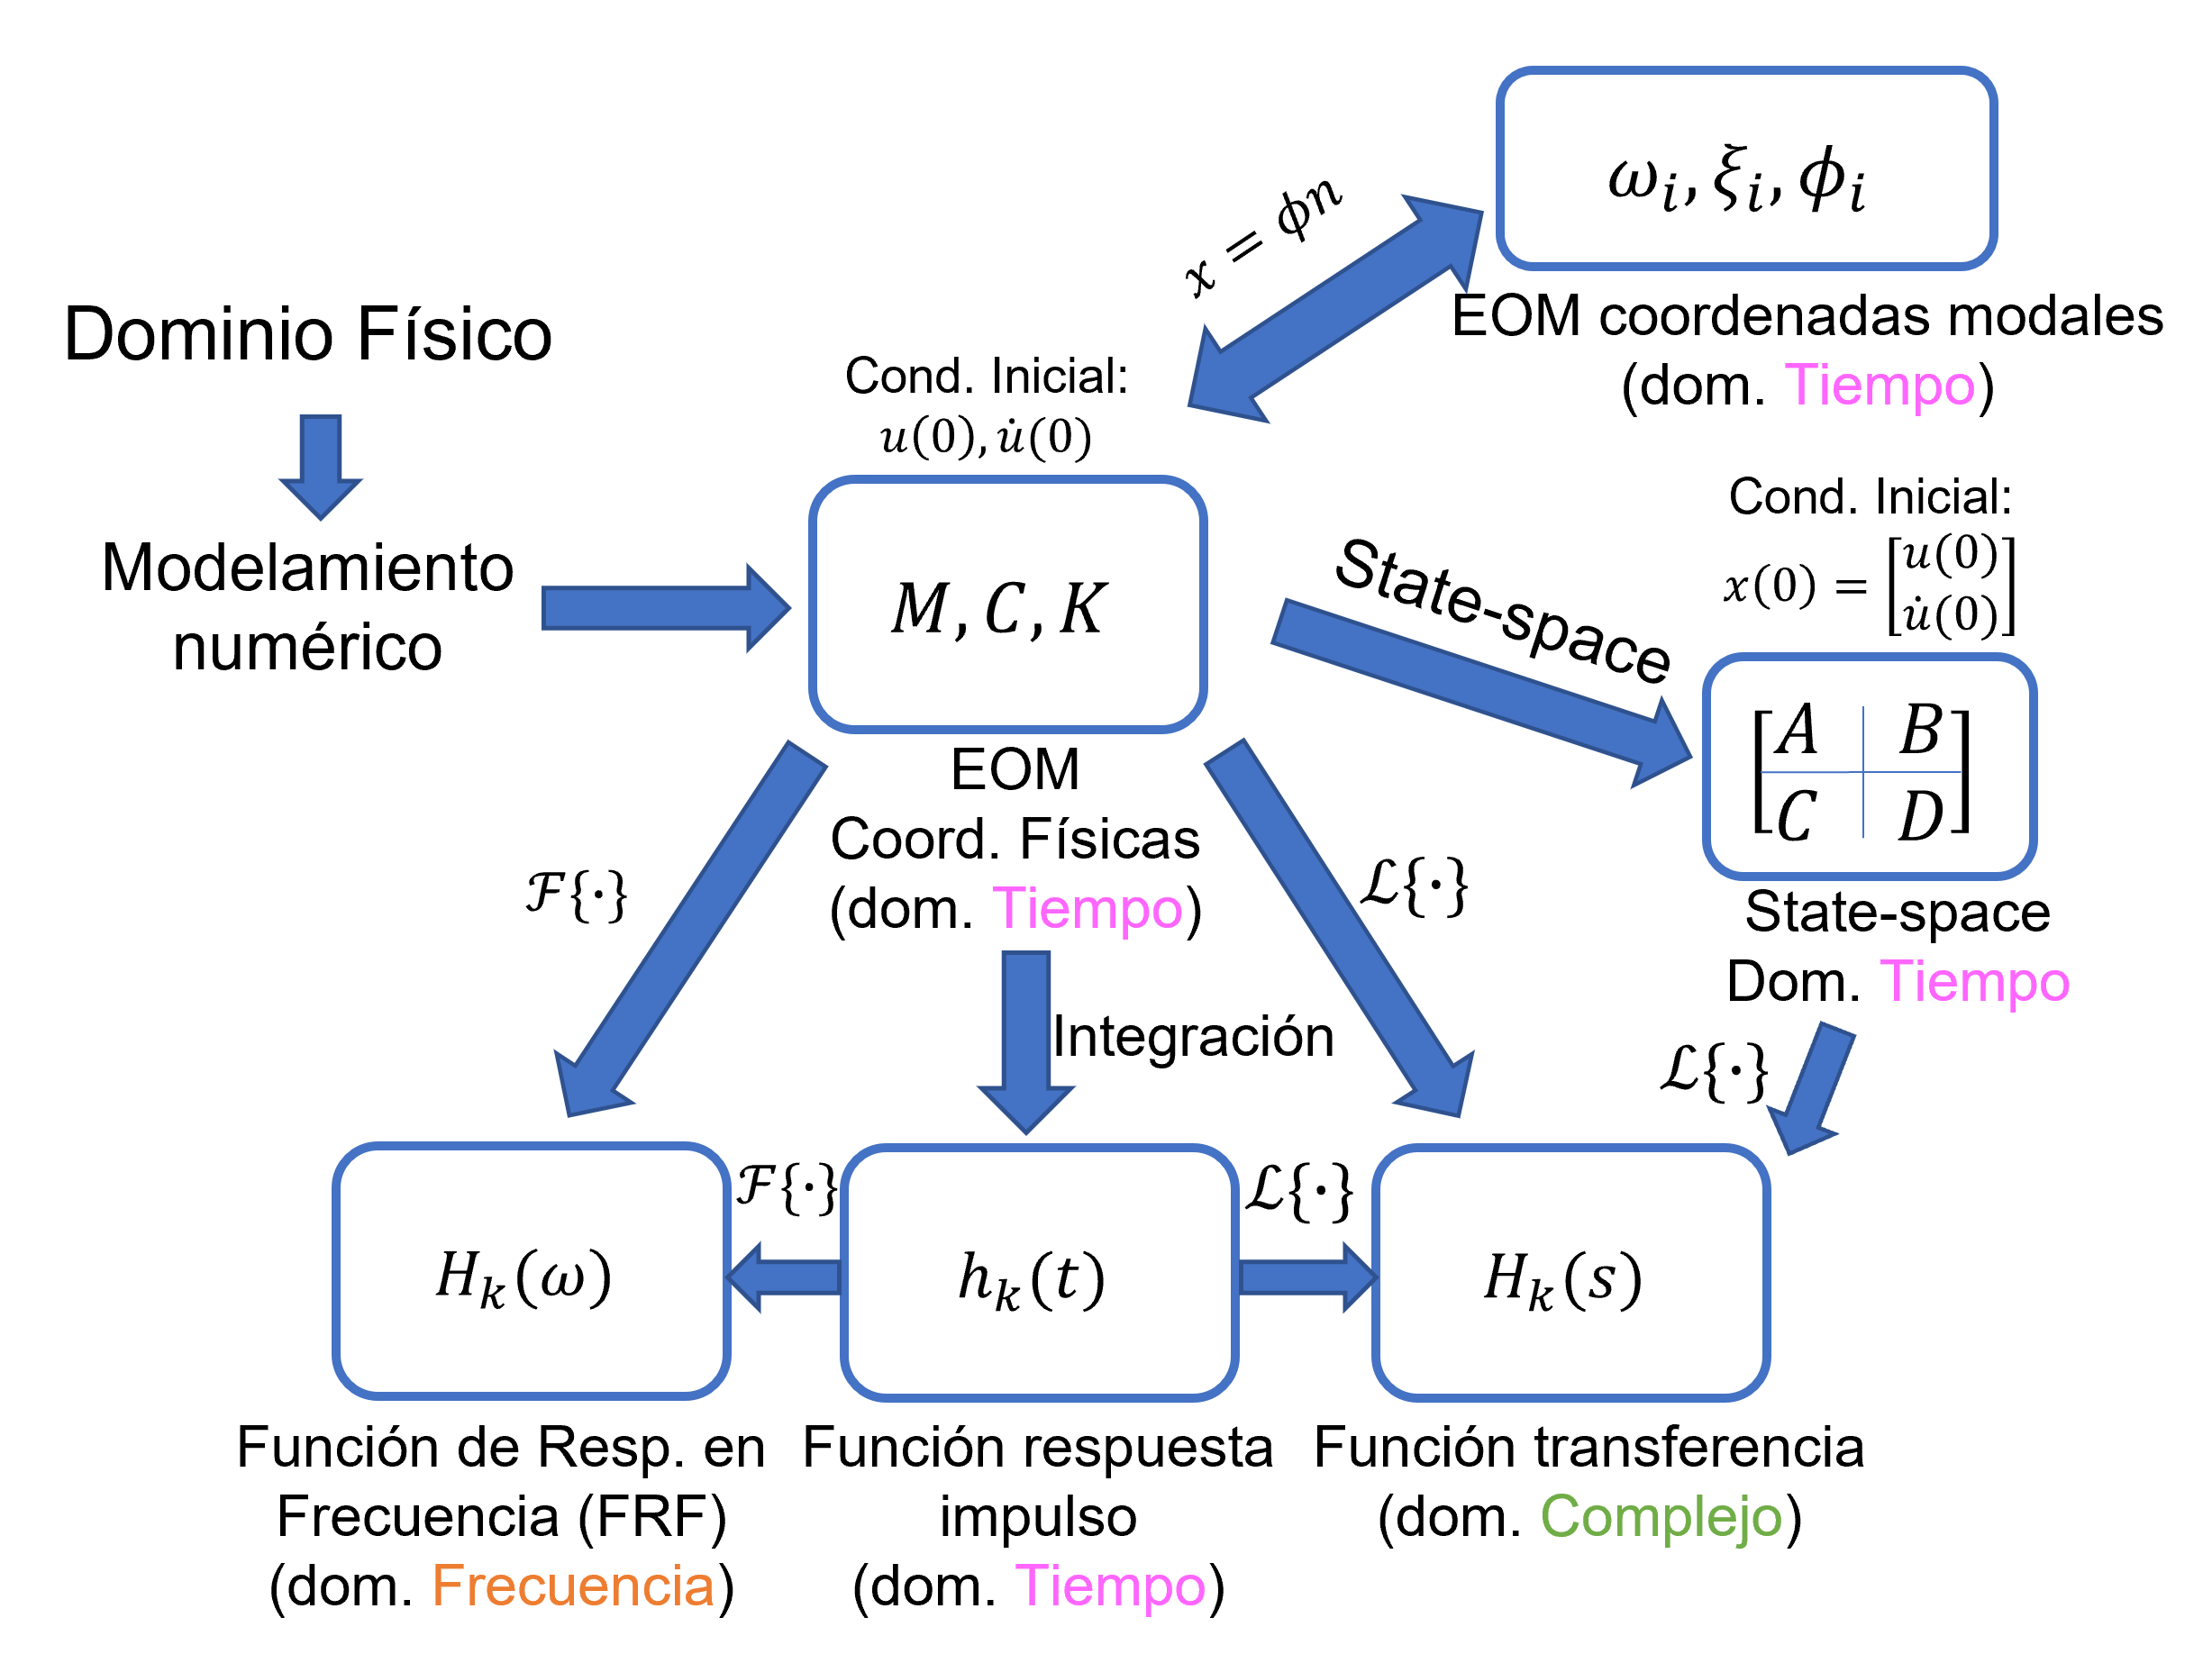
\includegraphics[scale=0.8]{modelos.png}
    \caption{Relaciones entre distintas representaciones de modelos de sistemas dinámicos.}
\end{figure}

\section{Función de transferencia de un sistema de 1GDL}
\begin{figure}[H]
\centering
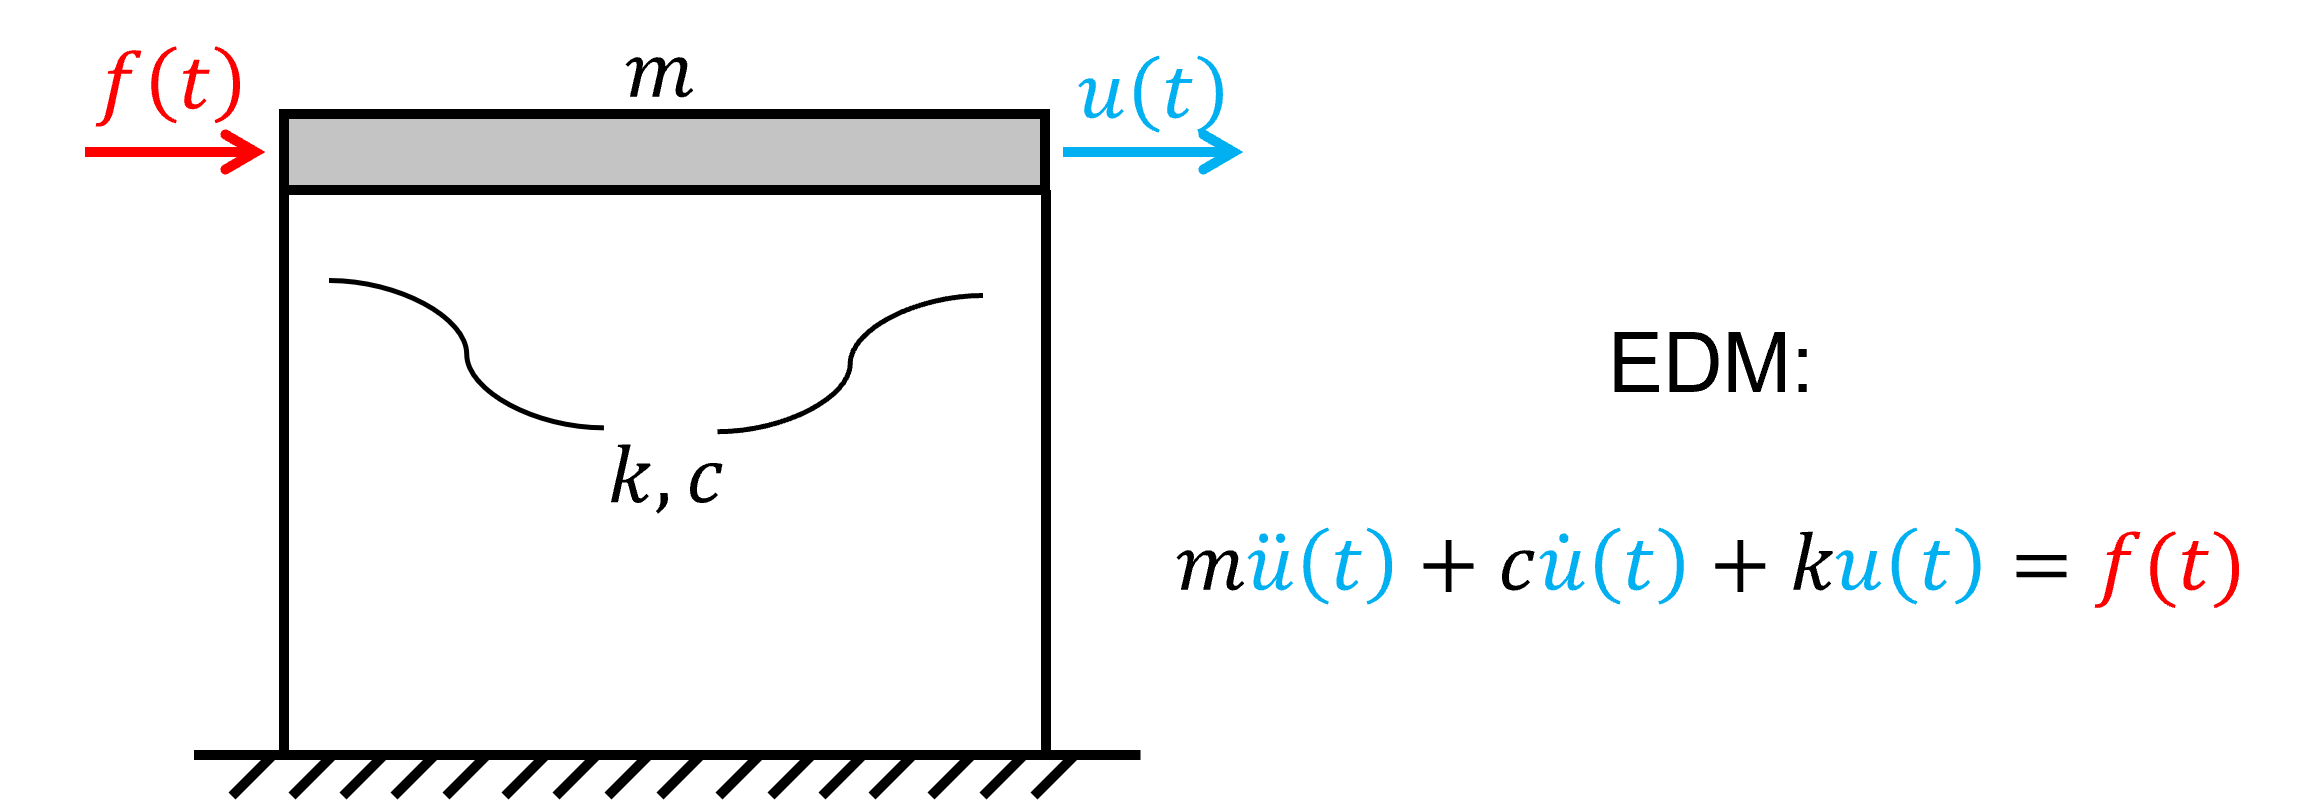
\includegraphics[scale=0.7]{edm.png}
\end{figure}
\underline{Problema}: Dada la EDM de un sistema estructural 1GDL, determinar su función de transferencia $H(s)$\\ 
\par Notación: 
\begin{align*}
    U(s) &= \mathcal{L}\{u(t)\}~: \text{respuesta (dominio complejo)}\\
    F(s) &= \mathcal{L}\{f(t)\} ~: \text{input (dominio complejo)}
\end{align*}

Asumiendo reposo: $u(0)=\dot{u}(0)=0$

\begin{align*}
    m\ddot{u}+c\dot{u}+ku &= f(t) ~/\color{red}{\mathcal{L}\{\cdot\}}\\
    m\mathcal{L}\{\ddot{u}\}+c\mathcal{L}\{\dot{u}\}+k\mathcal{L}\{u\} &= \mathcal{L}\{f\}\\
    ms^2U(s)+csU(s)+kU(s) &= F(s)\\
    (ms^2+cs+k)U(s) &= F(s)
\end{align*}
\begin{align*}
    \Longrightarrow H(s) = \frac{U(s)}{F(s)}&=\frac{1}{ms^2+cs+k} ~\text{: TF del sistema de 1GDL}
\end{align*}

Aparte: Dada la entrada $F(s)$ y la TF $H(s)$, la salida es $U(s) = H(s)F(s)$
\begin{figure}[H]
\centering
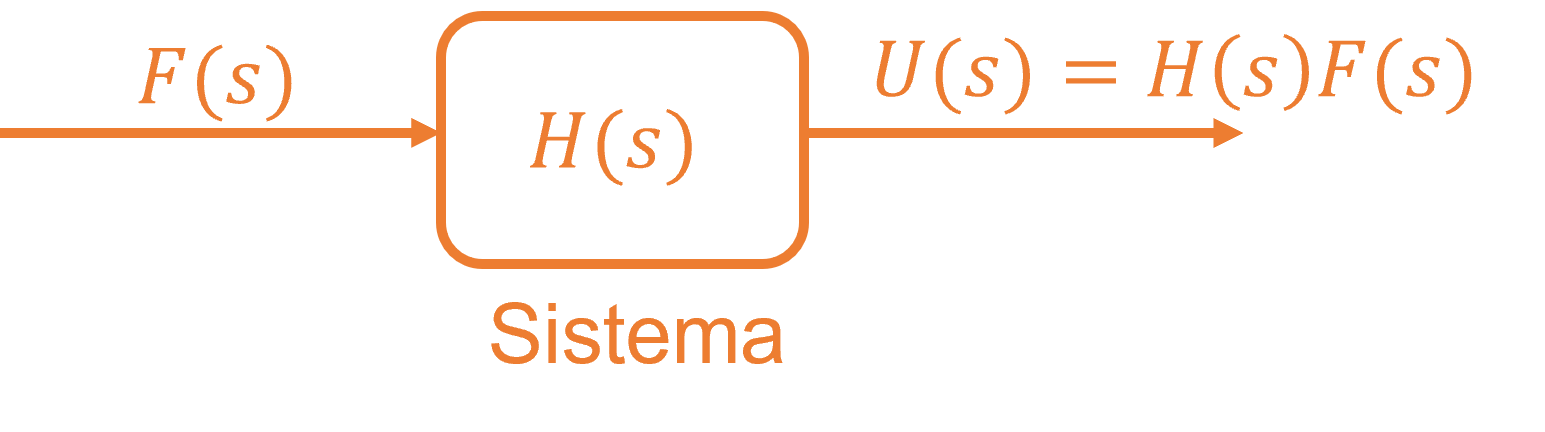
\includegraphics[scale=0.7]{hs.png}
\end{figure}

Desde la TF del sistema:
\begin{align*}
    H(s) &= \frac{1}{ms^2+cs+k} ~\color{red}{\frac{1/m}{1/m}}\\
    &= \frac{1/m}{s^2+2\xi\omega_ns+\omega_n^2}
\end{align*}
\begin{itemize}
    \item $\xi$: razón de amortiguamiento
    \item $\omega_n$: frecuencia natural
\end{itemize}

¿Cómo se obtienen los polos? $\Longrightarrow$ Calcular las raíces del polinomio del denominador:
\begin{align*}
    s^2+2\xi\omega_ns+\omega_n^2=0 ~\text{: Ecuación característica}
\end{align*}
\begin{align*}
     s_{1,2}=-\xi\omega_n\pm\omega_n\sqrt{1-\xi^2}j\\
     s_{1,2}=-\xi\omega_n\pm\omega_dj ~\text{: Polos del sistema de 1GDL}
\end{align*}

¿Es estable? $\Longrightarrow$ Depende del valor de $\xi$:
\begin{itemize}
    \item $\xi>0, ~ Re(s_{1,2}<0\Longrightarrow$ Estable asintóticamente
    \item $\xi<0, ~ Re(s_{1,2}>0\Longrightarrow$ Inestable
    \item $\xi=0, ~ Re(s_{1,2}=0\Longrightarrow$ ``Estable''
\end{itemize}

Además, el sistema oscila sí y solo si $\omega_d>0\Longrightarrow \omega_n>0$: propiedad del sistema dinámico.\\
Si $\xi>0, ~ \omega_n>0$:
\begin{figure}[H]
\centering
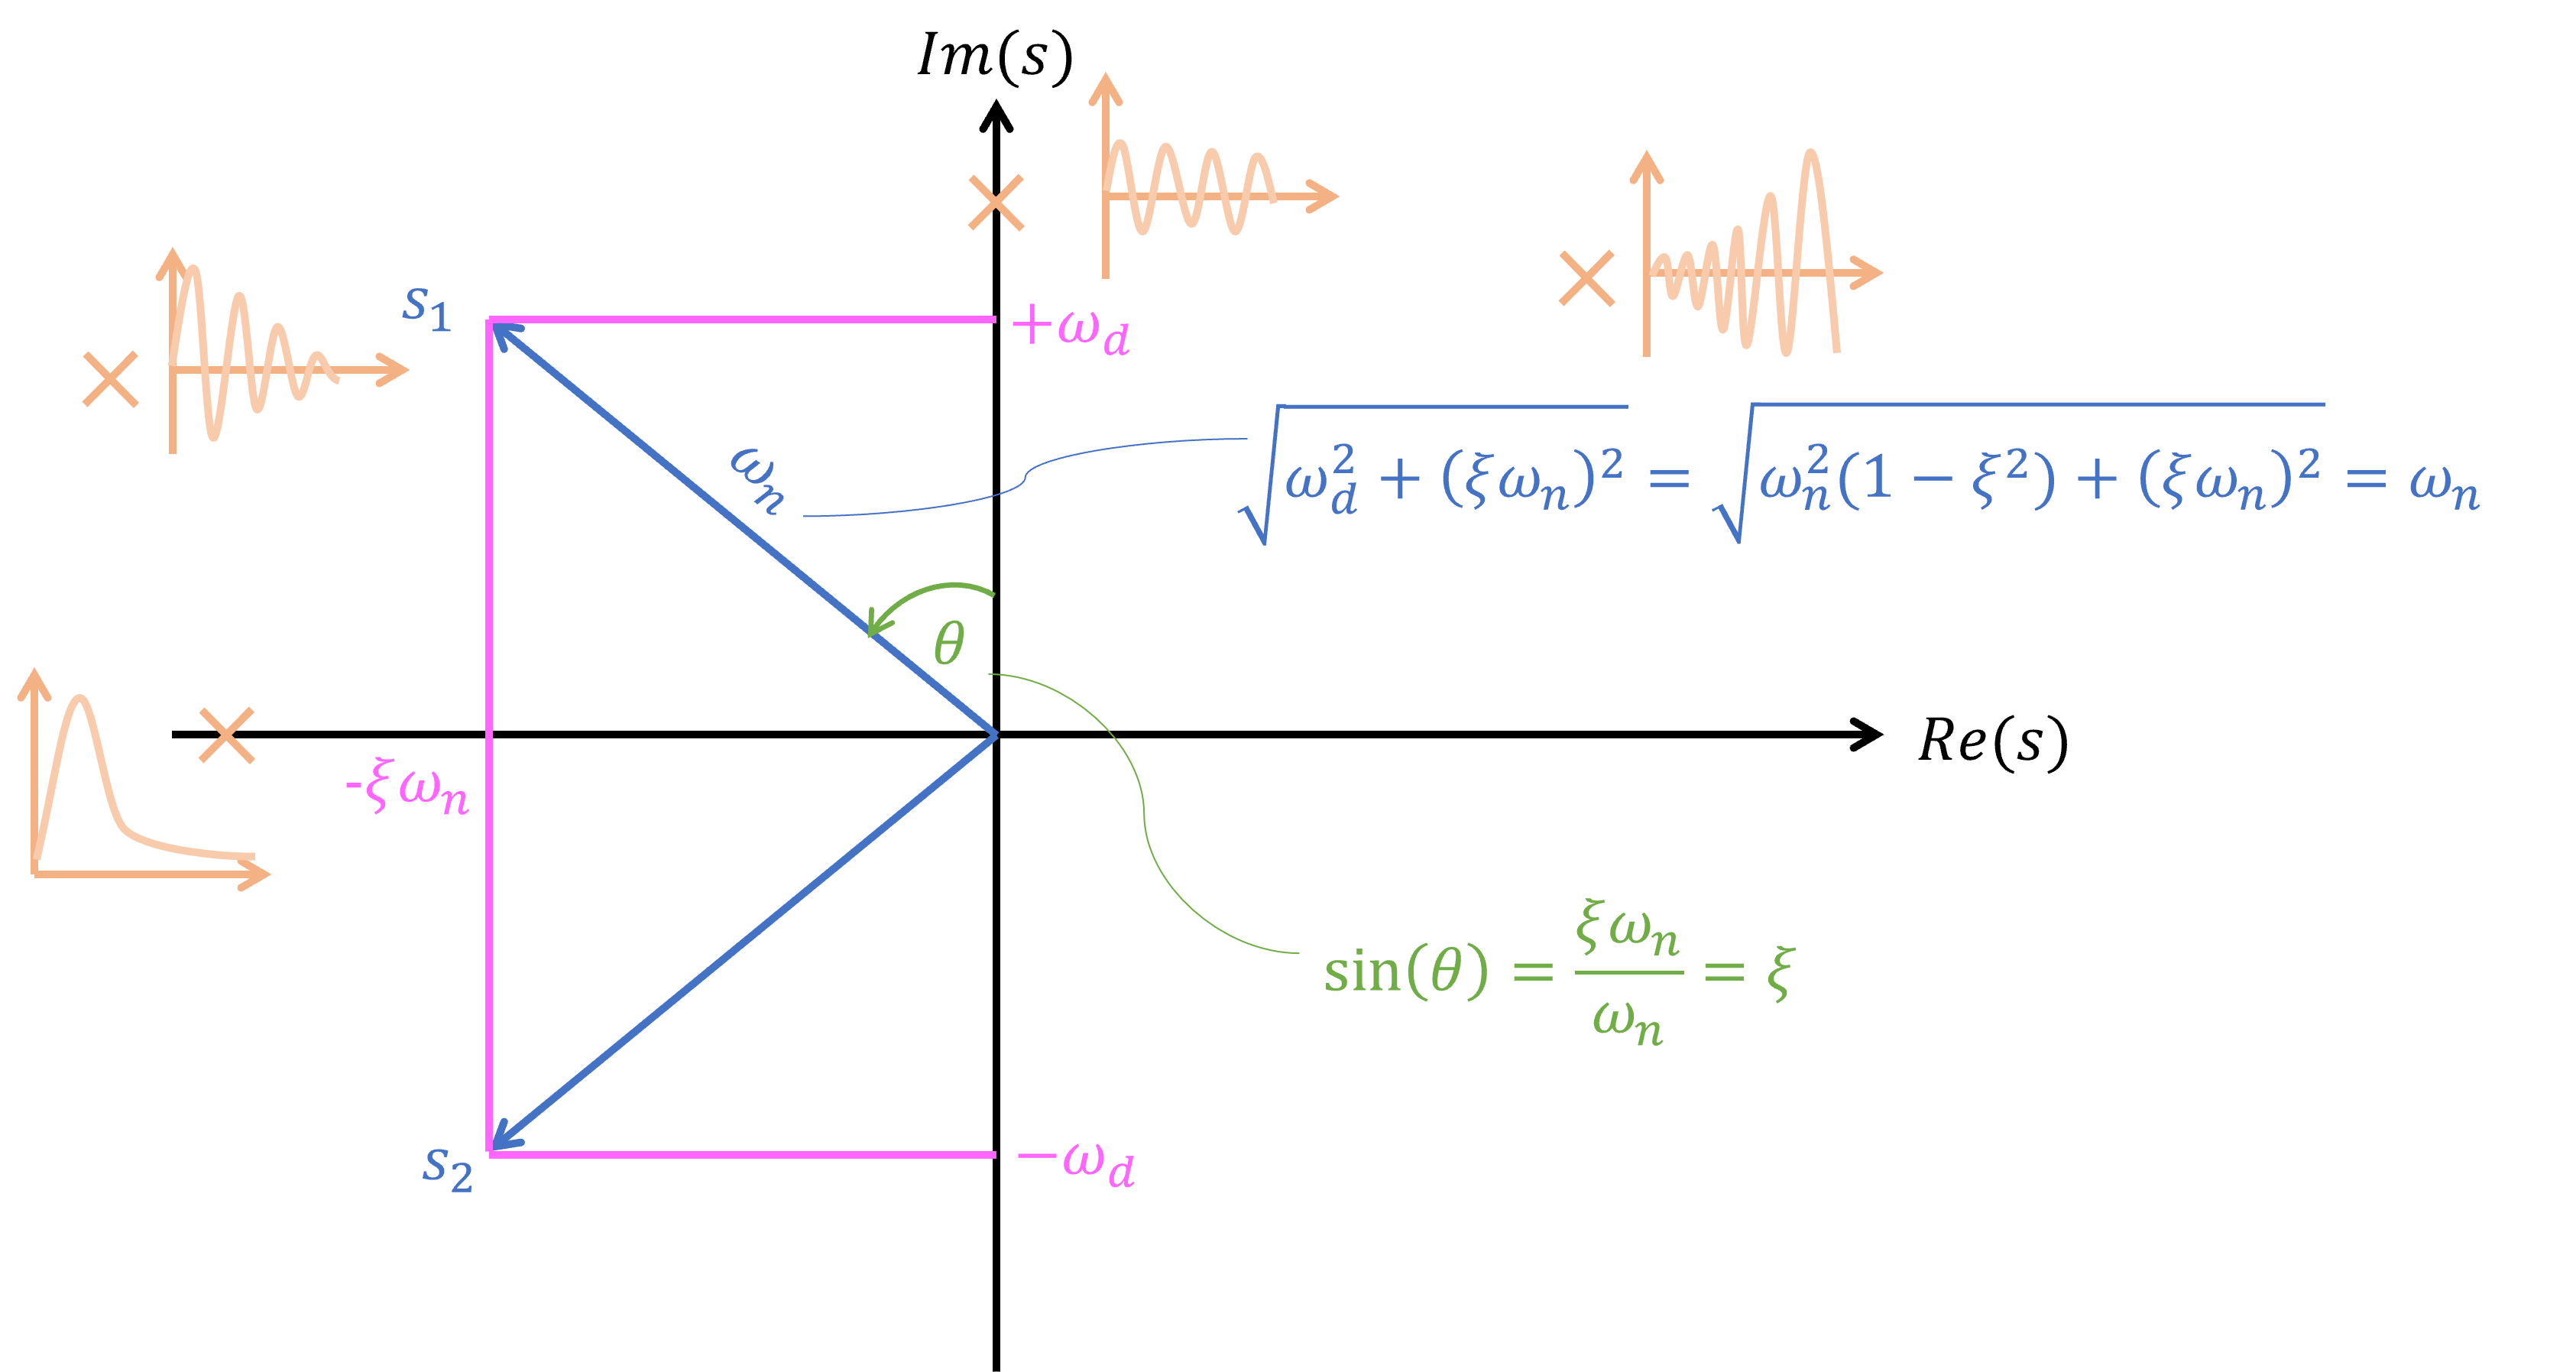
\includegraphics[scale=0.6]{estabilidad.png}
\end{figure}

% La Función de Respuesta en Frecuencia se obtiene a través de aplicar la transformada de Fourier:
%\begin{align*}
%    H(\omega)=\mathcal{F}\{h(t)\}
%\end{align*}

Notar que el FRF se puede obtener al reemplazar $s=j\omega$ en la TF:
\begin{align*}
    H(\omega)=H(s)\bigg|_{s=j\omega}
\end{align*}

\underline{Ejemplo}: Sistema de 1GDL
\begin{align*}
    \text{EOM: }~m\ddot{u}+c\dot{u}+ku=f(t)
\end{align*}
\begin{align*}
    \Longrightarrow \text{TF: }&~ H(s)=\frac{1}{ms^2+cs+k}=\frac{1/m}{s^2+(c/m)s+k/m}\\
    \Longrightarrow \text{FRF: }&~ H(\omega)=H(s)\bigg|_{s=j\omega}=\frac{1}{(k=m\omega^2)+j\omega c}
\end{align*}
\begin{align*}
    H(\omega)=\frac{1}{(j\omega-\lambda_1)(j\omega-\lambda_1^*)}
\end{align*}
\begin{itemize}
    \item $\{\}^*$: conjugado del número complejo
\end{itemize}
\begin{align*}
    \lambda_1, \lambda_1^*=-\xi\omega_n\pm\omega_n\sqrt{1-\xi^2}~\text{: polos del sistema}
\end{align*}

\section{Función de transferencia de un sistema de MGDL}
La TF de un sistema dinámico de MGDL se obtiene aplicando la transformada de Laplace a la EDM:

\begin{align*}
    \tenq{M}\tend{\ddot{u}}(t)+\tenq{C}\tend{\dot{u}}(t)+\tenq{K}\tend{u}(t)&=\tend{F}(t) ~/\mathcal{L}\{\cdot\}\\
    \Longrightarrow s^2\tenq{M}\tend{U}(s) + s\tenq{C}\tend{U}(s) +\tenq{K}\tend{U}(s) &= \tend{F}(s)\\
    \Longrightarrow\left[s^2\tenq{M}+s\tenq{C}+\tenq{K} \right]\tend{U}(s)&=\tend{F}(s) \\
    \Longrightarrow \tenq{H}(s) = \frac{\tenq{U}(s)}{\tenq{F}(s)} = =\left[s^2\tenq{M}+s\tenq{C}+\tenq{K} \right]^{-1} 
\end{align*}

Donde 
\begin{align*}
    \tend{F}(s) &= \mathcal{L}\{\tend{f}(t)\} ~: \text{input en dominio complejo (excitación)}\\
    \tend{U}(s) &= \mathcal{L}\{\tend{u}(t)\}~: \text{output en dominio complejo (respuesta)}\\
    \tenq{H}(s) &= \left[s^2\tenq{M}+s\tenq{C}+\tenq{K} \right]^{-1} ~:\text{TF para un sistema MGDL}
\end{align*}

Notar que para encontrar los polos se debe resolver las raíces polinomio:
\begin{align*}
    s^2\tenq{M}+s\tenq{C}+\tenq{K} = \tend{0} ~/ \text{$\cdot\tend{\phi}$ yasumiendo $\tenq{C}=\tenq{0}$} \\
    \Longrightarrow (s^2\tenq{M}+\tenq{K})\tend{\phi} = \tend{0} ~\text{: Problema de valores propios generalizado}
\end{align*}

\subsection{Representación en Variables de Estado (State-Space)}

La representación espacio-estado reduce la EDM a ecuaciones diferenciales ordinarias cuyas matrices contienen toda la información dinámica del sistema.

\begin{align*}
    \text{EDM: }~\tenq{M}\tend{\ddot{u}}+\tenq{C}\tend{\dot{u}}+\tenq{K}\tend{u}&=\tenq{G}\tend{p}(t) 
\end{align*}

\begin{align*}
\left .
\begin{array}{rr}
\tend{\dot{x}}=\tenq{A_s}\tend{x}+\tenq{B_s}\tend{p}\\
\tend{y}=\tenq{C_s}\tend{x}+\tenq{D_s}\tend{p} 
\end{array}
\right \} \Longrightarrow 
\begin{array} {|r|r|}
  \hline A & B \\
  \hline C & D \\
  \hline 
\end{array}
\end{align*}

\begin{figure}[H]
\centering
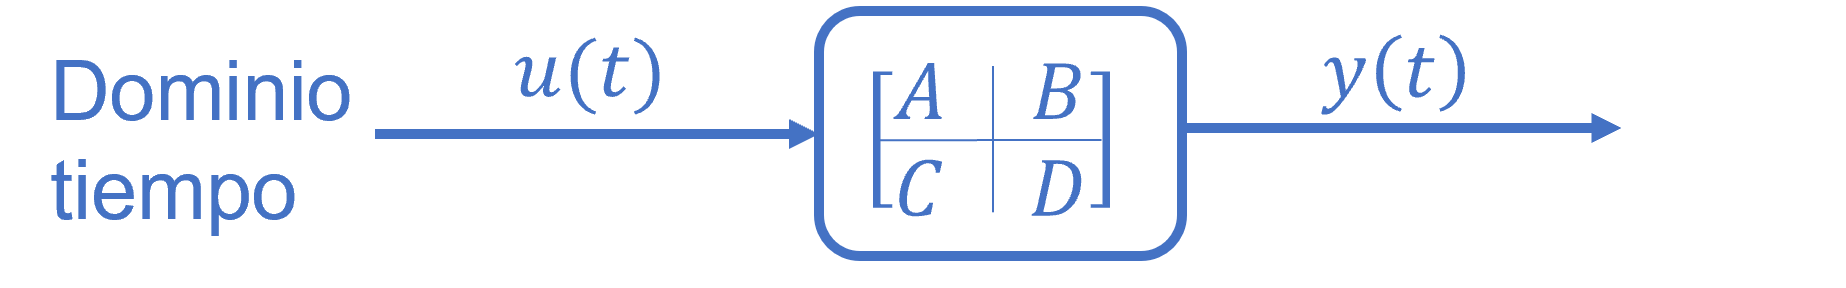
\includegraphics[scale=0.7]{SS.png}
\end{figure}

\underline{Ecuación de estado}

\begin{align*}
    \tend{\dot{x}}=\tenq{A_s}\tend{x}+\tenq{B_s}\tend{p}
\end{align*}

Donde:
\begin{itemize}
    \item Vector de Estado: $\tend{x}=\begin{bmatrix}\tend{u} \\ \tend{\dot{u}}\end{bmatrix} \Longrightarrow \tend{\dot{x}}=\begin{bmatrix}\tend{\dot{u}}\\ \tend{\ddot{u}}\end{bmatrix}$
    \item Matriz de estado: $\tenq{A_s}=\begin{bmatrix}\tenq{0} & \tenq{I}\\ -\tenq{M}^{-1}\tenq{K} & -\tenq{M}^{-1}\tenq{C}\end{bmatrix}$
    \item Matriz de influencia de excitación: $\tenq{B_s}=\begin{bmatrix}\tenq{0}\\ \tenq{M}^{-1}\tenq{G}\end{bmatrix}$
\end{itemize}

\underline{Ecuación de respuesta} \\

\begin{align*}
    \tend{y}=\tenq{C_s}\tend{x}+\tenq{D_s}\tend{p}
\end{align*}

Donde (este es un ejemplo):
\begin{itemize}
    \item Vector de respuesta: $\tend{y}=\begin{bmatrix}\tend{u} \\ \tend{\dot{u}}\\ \tend{\ddot{u}}\end{bmatrix}$

    \item $\tenq{C_s}=\begin{bmatrix}\tenq{I} & \tenq{0}\\
    \tenq{0} & \tenq{I}\\ 
    -\tenq{M}^{-1}\tenq{K} & -\tenq{M}^{-1}\tenq{C}\end{bmatrix}$
    \item ``Feedthrough'': $\tenq{D_s}=\begin{bmatrix}\tenq{0}\\
    \tenq{0}\\ \tenq{M}^{-1}\tenq{G}\end{bmatrix}$
\end{itemize}

\subsection{Relación entre State-Space y TF}

Asumiendo condiciones iniciales de reposo: $\tend{x}(0) = \tend{0} \longrightarrow \text{Estados}$\\

Entonces, aplicando la transformada de laplace a la ecuación de estado:
\begin{align*} \label{eq:ss2tf_1}
    \tend{\dot{x}}&=\tenq{A_s}\tend{x}+\tenq{B_s}\tend{p} ~/\mathcal{L}\{\cdot\}\\
    \Longrightarrow s\tend{X}(s)&= \tenq{A_s}\tend{X}(s)+\tenq{B_s}\tend{P}(s)\\
    \Longrightarrow (s\tenq{I}-\tenq{A_s})\tend{X}(s)&=\tenq{B_s}\tend{P}(s)
\end{align*}
\begin{align}
    \Longrightarrow \tend{X}(s)&=(s\tenq{I}-\tenq{A_s})^{-1}\tenq{B_s}\tend{P}(s)
\end{align}

Luego, aplicando la transformada de Laplace a la ecuación de respuesta:

\begin{align*}
    \tend{y}(t)=\tenq{C_s}\tend{x}+\tenq{D_s}\tend{p} ~/\mathcal{L}\{\cdot\}\\
\end{align*}
\begin{align}\label{eq:ss2tf_2}
    \Longrightarrow \tend{Y}(s)&=\tenq{C_s}\tend{X}(s)+\tenq{D_s}\tend{P}(s)
\end{align} 

Reemplazando la ecuación \ref{eq:ss2tf_1} en \ref{eq:ss2tf_2}:
\begin{align*}
    \tend{Y}(s)&=\tenq{C_s}(s\tenq{I}-\tenq{A_s})^{-1}\tenq{B_s}\tend{P}(s)+\tenq{D_s}\tend{P}(s)\\
    \tend{Y}(s)&=[\tenq{C_s}(s\tenq{I}-\tenq{A_s})^{-1}\tenq{B_s}+\tenq{D_s}]\tend{P}(s)\\
    \Longrightarrow \tenq{H}(s)&=\tenq{C_s}(s\tenq{I}-\tenq{A_s})^{-1}\tenq{B_s}+\tenq{D_s}
\end{align*}

\underline{Aparte}: Asumiendo $\tenq{D_s}=0$:
\begin{align*}
    \tenq{H}(s)&=\tenq{C_s}(s\tenq{I}-\tenq{A_s})^{-1}\tenq{B_s}\\
    \tenq{H}(s)&=\frac{1}{\det(s\tenq{I}-\tenq{A_s})}\tenq{C_s}\text{ adj}(s\tenq{I}-\tenq{A_s})\tenq{B_s} \\
    \Longrightarrow\det(s\tenq{I}-\tenq{A_s})&=0 ~\text{: Problema de valores propios de }\tenq{A_s}
\end{align*}

Por lo tanto, los Polos se pueden obtener por las raíces del polinomio del denominador de $\tenq{H}(s)$, o, por los valores propios de $\tenq{A_s}$.

\section{Función impulso (Delta Dirac)}
La función \textit{Delta de Dirac} se denota como:
\begin{align*}
    \delta(t)=   \left\{
\begin{array}{ll}
      +\infty & t=0 \\
      0 & t\neq 0 \\
\end{array} 
\right. 
\end{align*}

% Ale: O análogamente.
%\begin{align*}
%    \delta(t-\tau)=   \left\{
%\begin{array}{ll}
%      +\infty & t=\tau \\
%      0 & t\neq \tau \\
%\end{array} 
%\right. 
%\end{align*}

\begin{figure}[H]
\centering
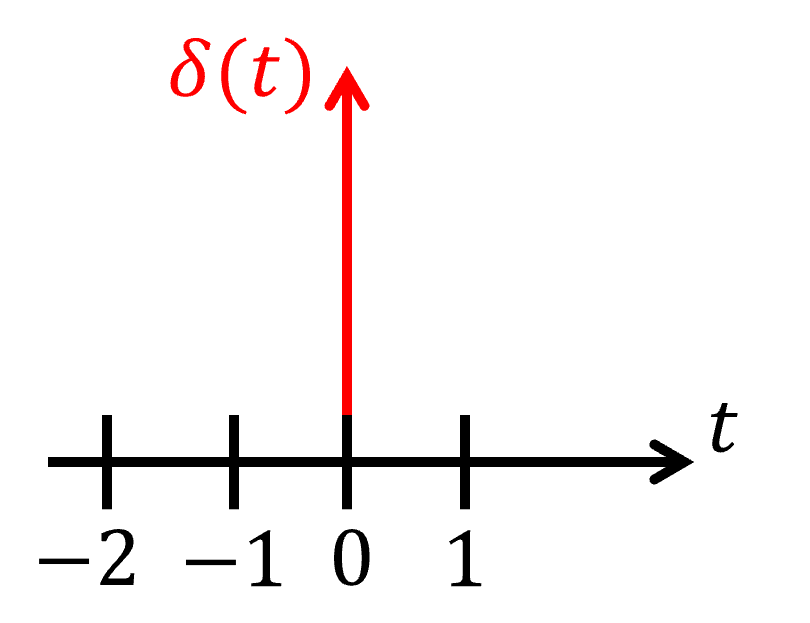
\includegraphics[scale=0.7]{delta.png}
\end{figure}

\underline{Propiedades}:
\begin{align*}
    \int_{-\infty}^{+\infty}\delta(t)dt=1 \quad &\text{Impulso unitario}\\
    \int_{-\infty}^{+\infty}f(t)\delta(t-T)dt=f(T) \quad &\text{Sampleo}
\end{align*}

\begin{figure}[H]
\centering
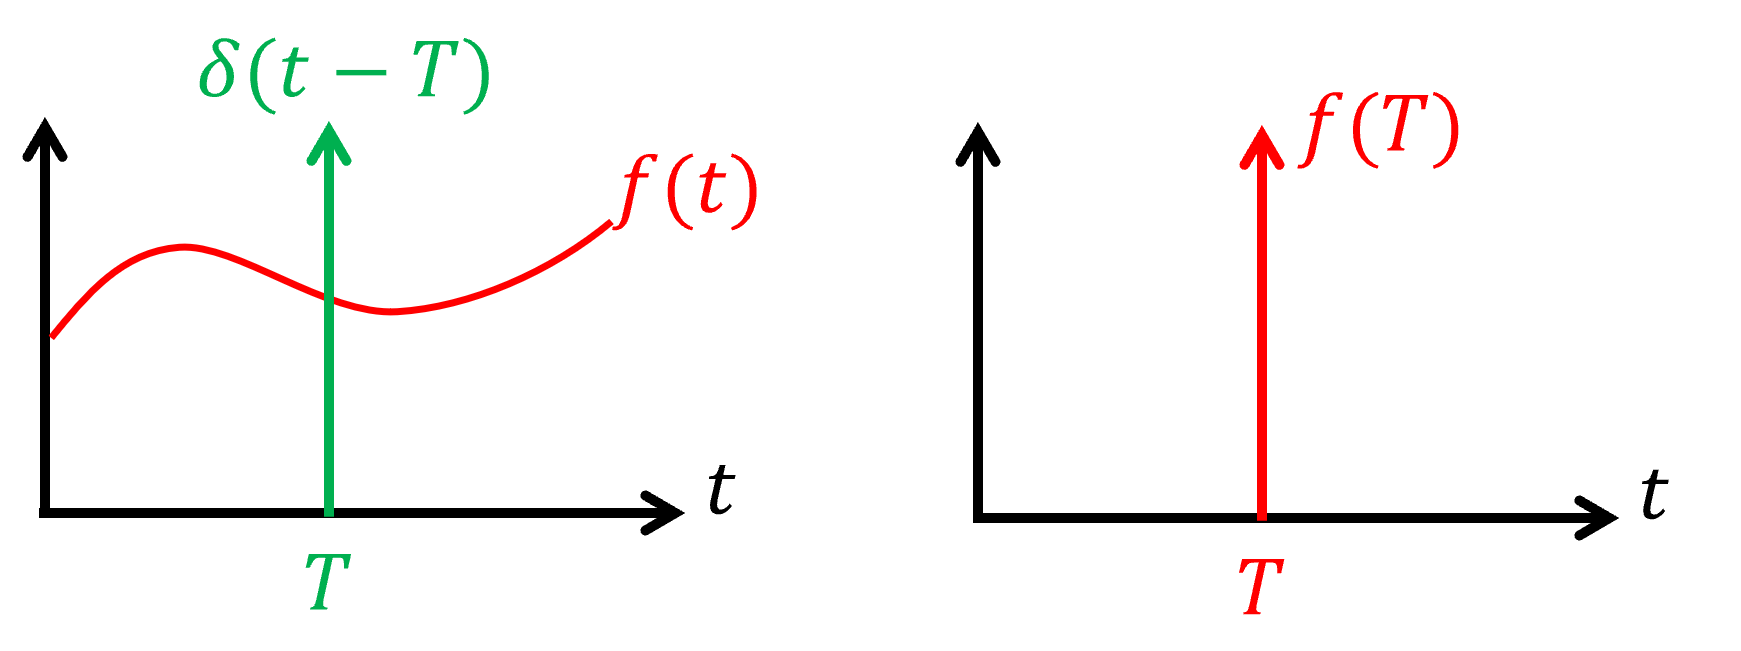
\includegraphics[scale=0.7]{dirac.png}
\end{figure}

\begin{align*}
    \Rightarrow f(T) = f(t)\ast\delta(t-T)
\end{align*}

\underline{Propiedad}: Sea $f(t)$ una función continua, entonces, se puede expresar como una integral de la convolución con la función $\delta(t)$.
\begin{align*}
    f(t)=\int_{-\infty}^{+\infty}f(\tau)\delta(t-\tau)d\tau 
\end{align*}

Esta superposición nos permite componer la función $f(t)$ como una suma infinita de impulsos unitarios con la función $\delta(t)$.
\begin{figure}[h]
\centering
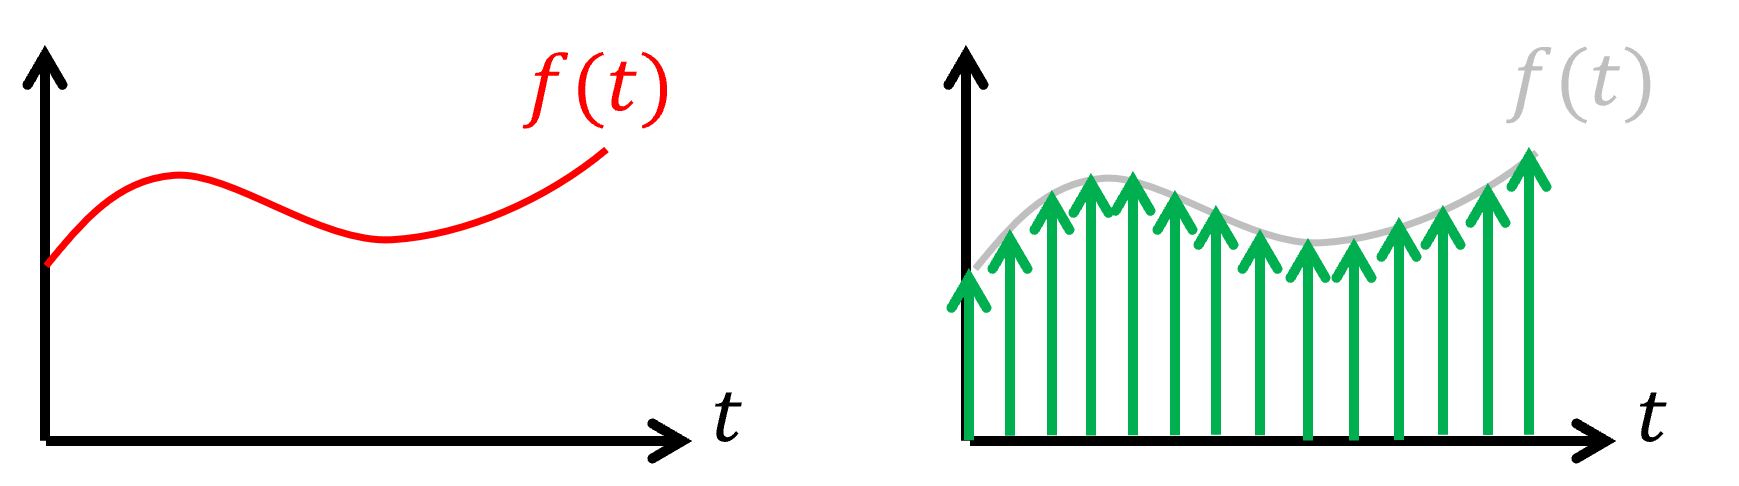
\includegraphics[scale=0.7]{suma_imp.png}
\end{figure}

\section{Función de respuesta a impulso unitario}
¿Cuál es la respuesta de un sistema cuando se le somete a un impulso unitario? 
\begin{figure}[H]
\centering
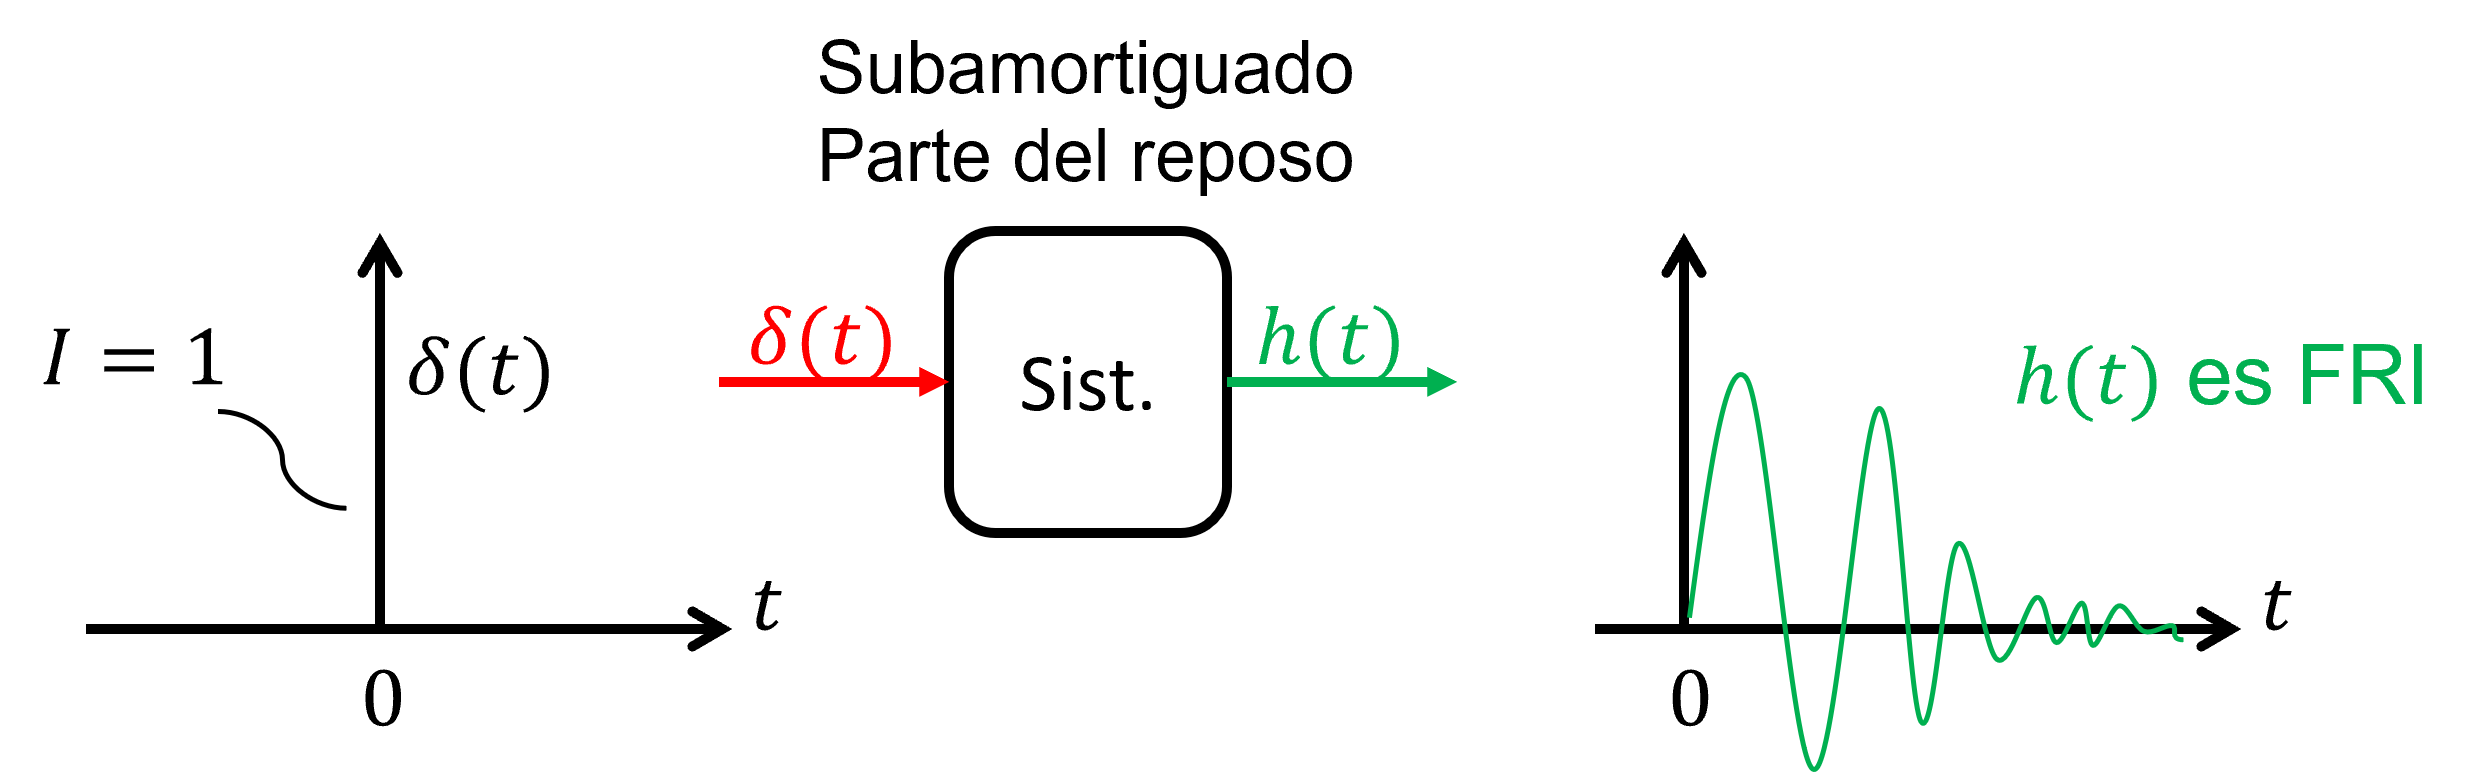
\includegraphics[scale=0.7]{FRI.png}
\end{figure}

\par Para sistemas estructurales ($\xi<1$), la ecuación de movimiento sometida a un impulso unitario:
\begin{align*}
    m\ddot{x}+c\dot{x}+kx=\delta(t)\\
    x(0)=0 \quad \dot{x}(0)=0
\end{align*}

La solución a esta ecuación es la Función de Respuesta Impulso (FRI) cuando el impulso se aplica en el tiempo $\tau = 0$:
\begin{align*}
    x(t)=h(t)=\frac{1}{m\omega_d}e^{-\xi\omega_nt}\sin{(\omega_dt)}, \quad t\geq0
\end{align*}

\noindent donde $\omega_n = \sqrt{\frac{k}{m}}$ es la frecuencia natural y $\omega_d = \omega_n \sqrt{1-\xi^2}$ es la frecuencia natural amortiguada. \\

Ahora, considere una excitación $u(t)$ continua. Se puede representar como un tren de impulsos:
\begin{figure}[H]
\centering
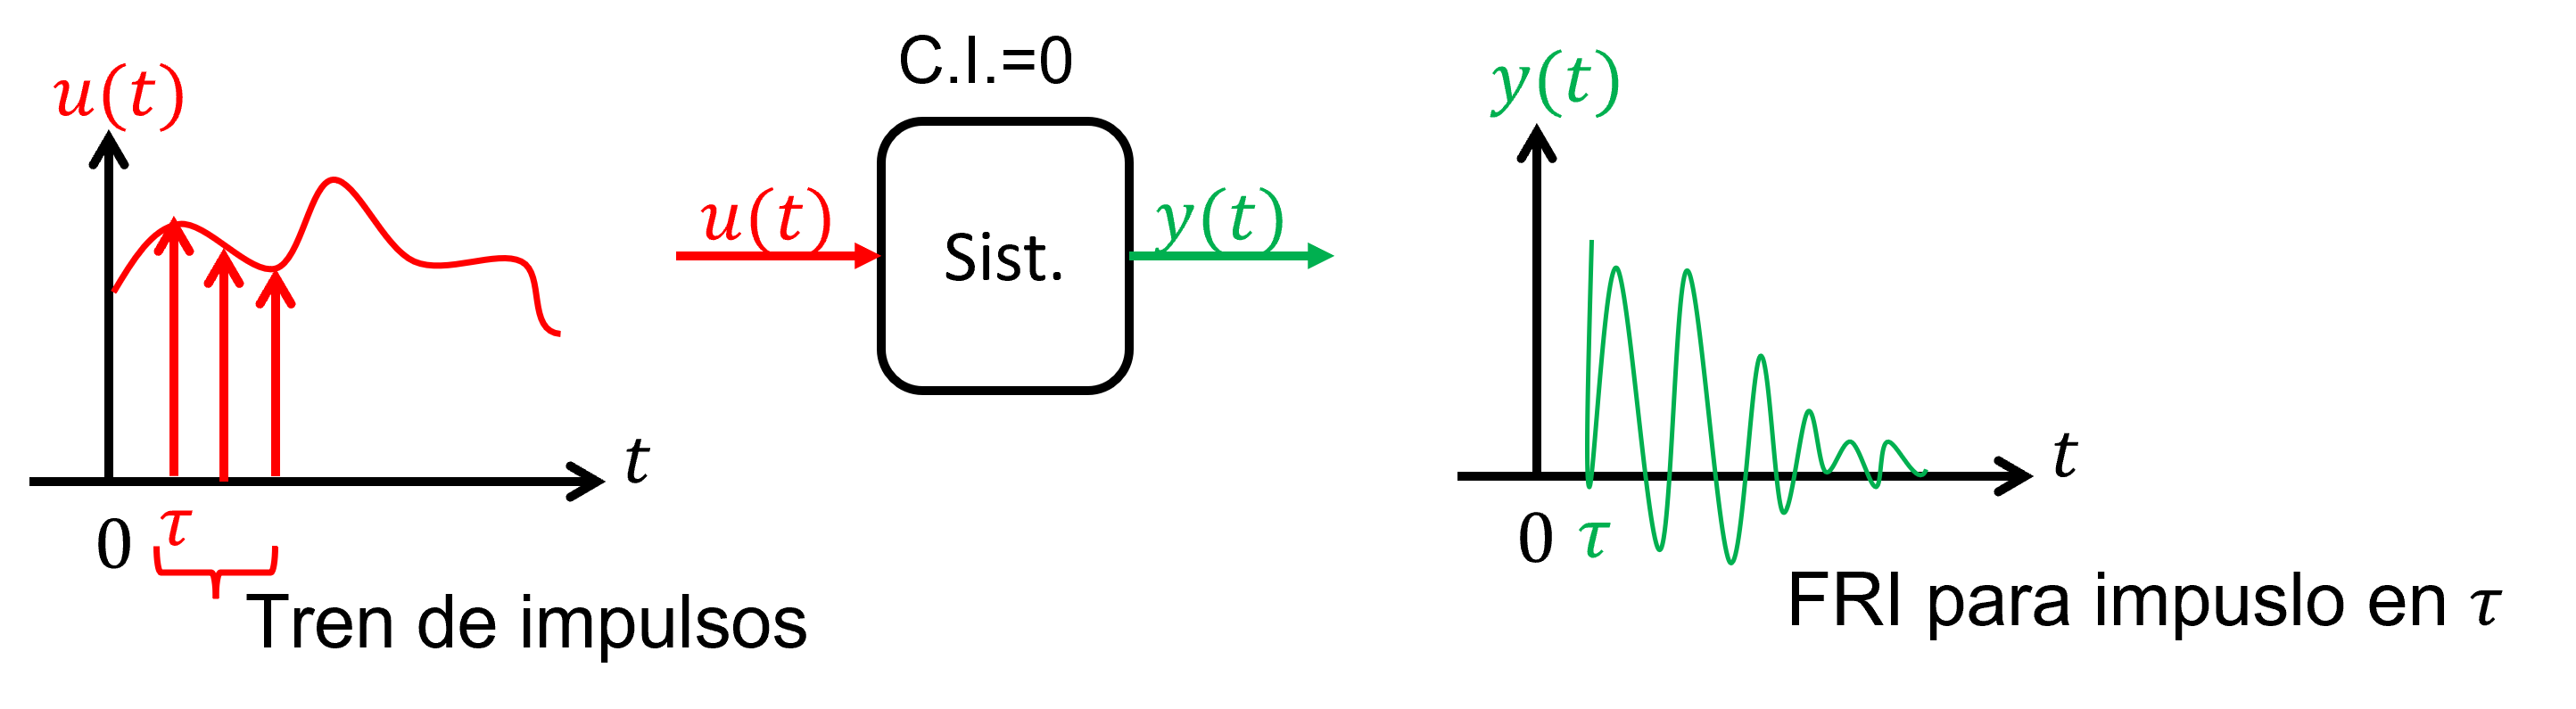
\includegraphics[scale=0.7]{FRI2.png}
\end{figure}
Notar que cada impulso genera una respuesta en el sistema $\delta(t-\tau)\longrightarrow h(t-\tau)$.

\begin{figure}[H]
\centering
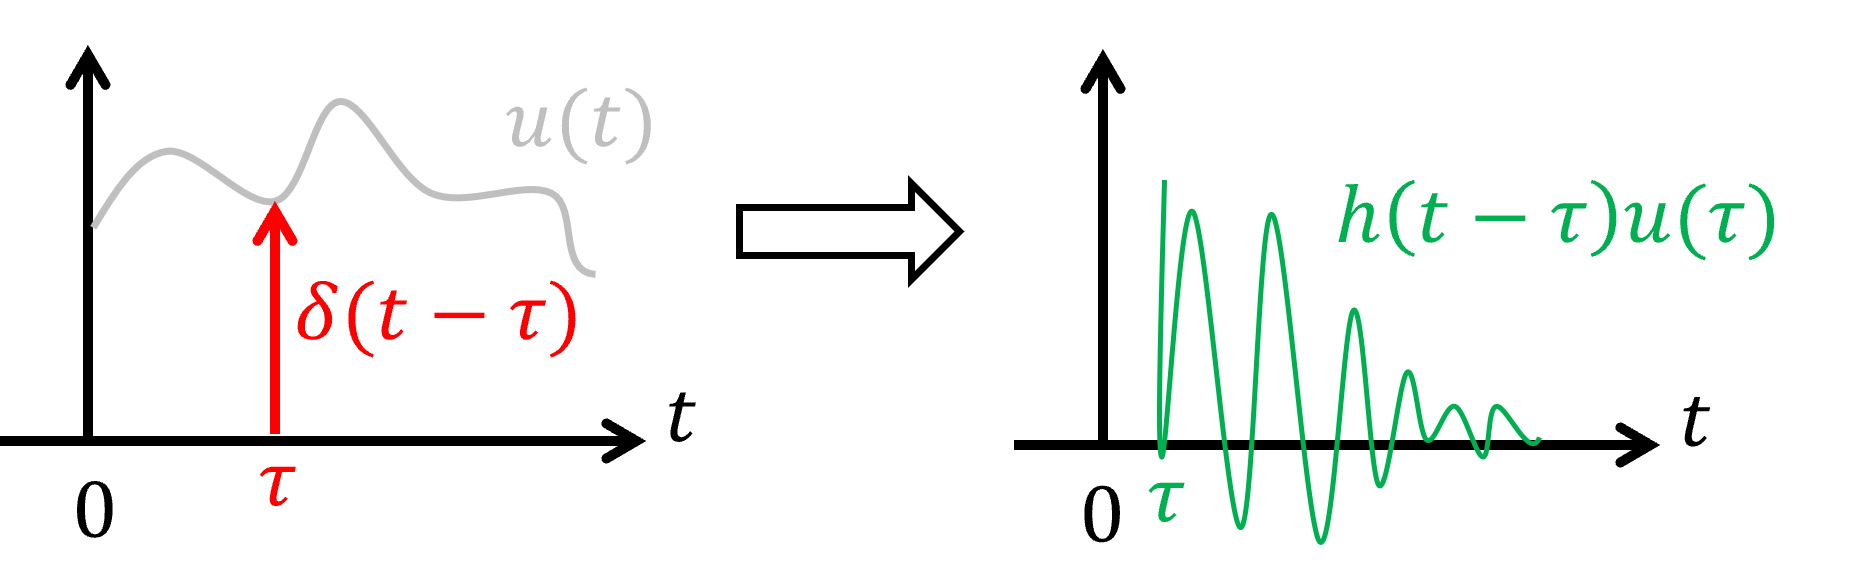
\includegraphics[scale=0.7]{FRI3.png}
/\end{figure}

La respuesta del sistema cuando se somete a este tren de impulsos se obtiene por superposición: 
\begin{align*}
    y(t)=\int_0^tu(\tau)h(t-\tau)d\tau \quad \text{``Integral de Duhamel''}\Rightarrow\text{Convolución}
\end{align*}

\underline{En resumen}: La respuesta analítica de un sistema LTI es la convolución entre el FRI $h(t)$ y la excitación $u(t)$.

\begin{align*}
    \Rightarrow y(t)=u(t)\ast h(t)
\end{align*}

\section{Transformada de Laplace}
\underline{Definición}: La transformada de Laplace de $f(t)$ es igual a:
\begin{align*}
    \mathcal{L}: ~ F(s)=\int_{-\infty}^{+\infty}f(t)e^{-\xi t}dt \quad \text{Transformada Bilateral (``two-sided'')}
\end{align*}

\noindent donde $s\in\mathbb{C}$, $s=\sigma+j\omega$, $j^2=-1$, $j$ es la unidad imaginaria.\\

\underline{Definición}: La transformada inversa de Laplace es igual a:
\begin{align*}
    \mathcal{L}^{-1}: ~ f(t)=\frac{1}{2\pi j}\int_{+\sigma-j\infty}^{+\sigma+j\infty}F(s)e^{st}ds
\end{align*}

La razón por la que se opta por trabajar con la variable de Laplace $s$ en lugar de utilizar el tiempo $t$ es la simplificación para obtener la respuesta. Al emplear la variable de Laplace, la respuesta se obtiene con multiplicaciones en vez de convoluciones.

\begin{figure}[H]
\centering
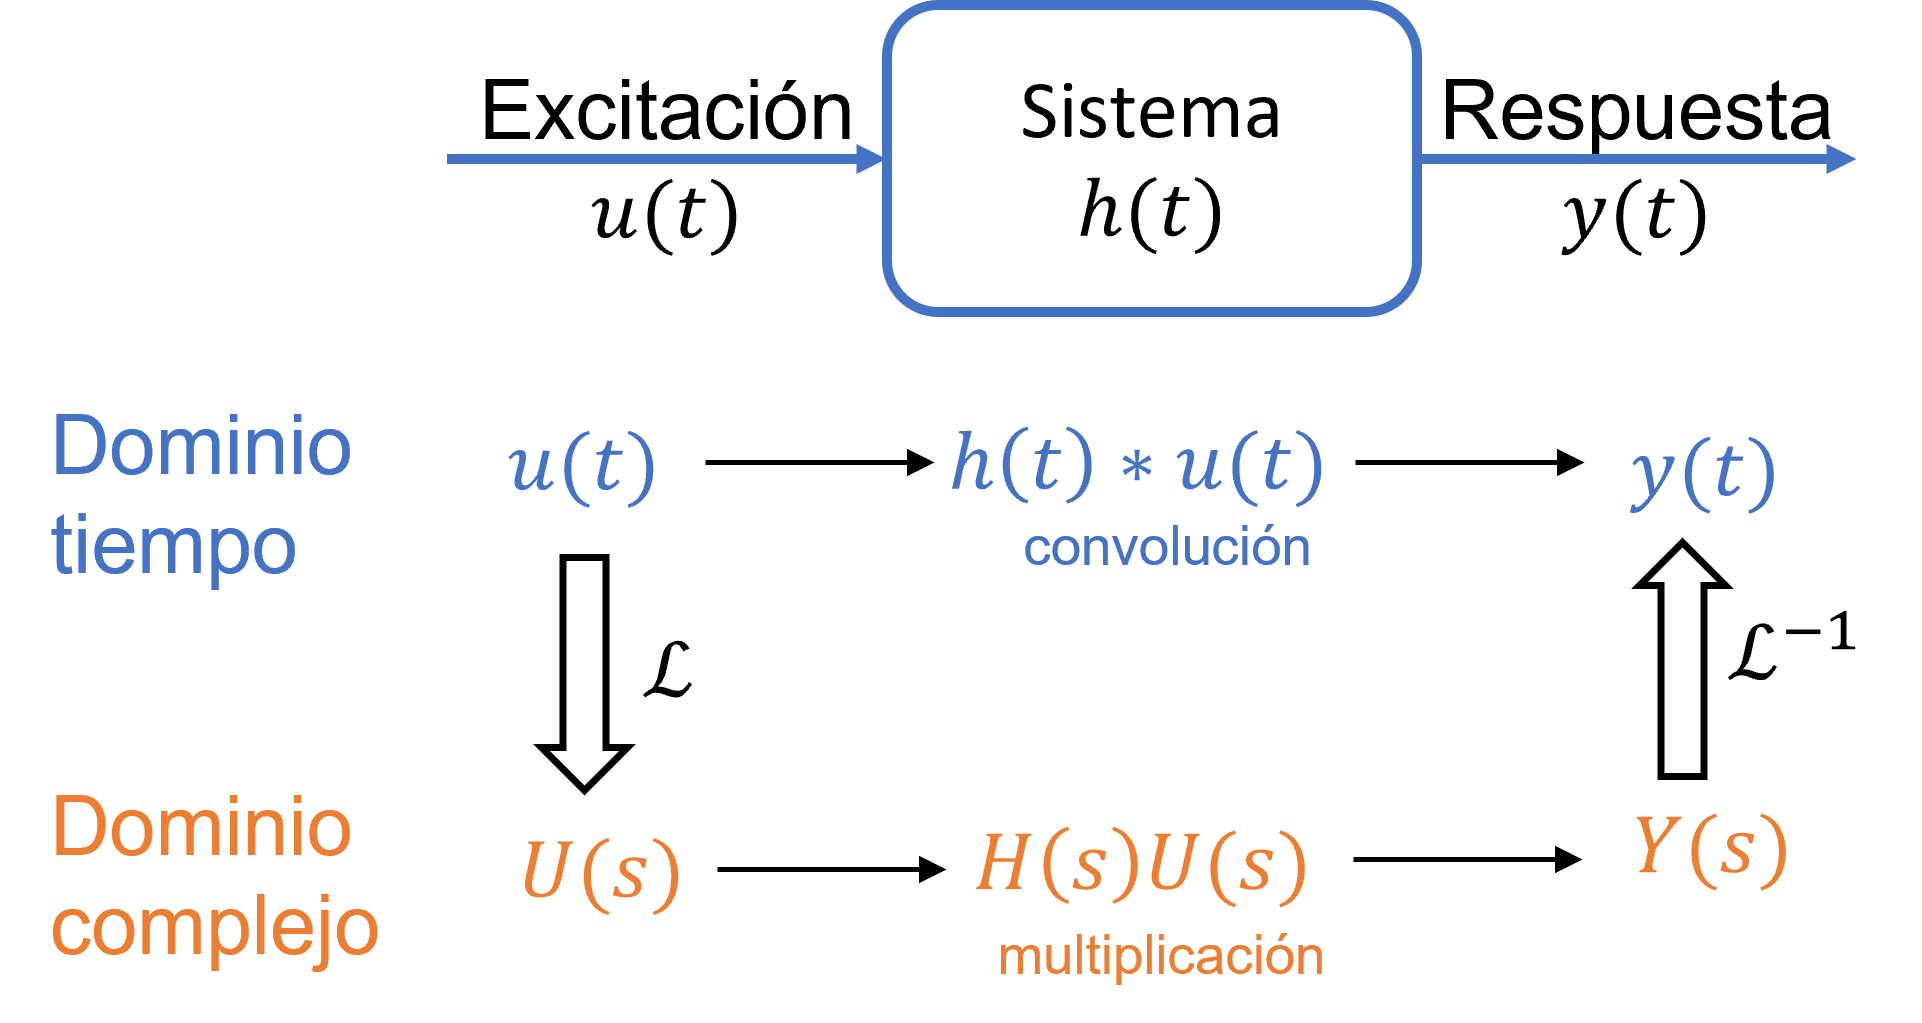
\includegraphics[scale=0.7]{laplace.png}
\end{figure}

Al obtener la respuesta ya sea por el dominio del tiempo o pasando por el dominio complejo, se obtiene exactamente el mismo resultado.
\begin{align*}
    y(t)=h(t)\ast u(t) \xRightarrow[]{\mathcal{L}} Y(s)=H(s)\cdot U(s)
\end{align*}
donde:
\begin{align*}
H(s)=\mathcal{L}\{h(t)\}=\int_0^{\infty}h(t)e^{-\xi t}dt \\
Y(s)=\mathcal{L}\{y(t)\}=\int_0^{\infty}y(t)e^{-\xi t}dt \\
U(s)=\mathcal{L}\{u(t)\}=\int_0^{\infty}u(t)e^{-\xi t}dt
\end{align*}
\begin{itemize}
    \item $h(t)$: Función de Respuesta Impulso (FRI)
    \item $H(s)$: Función de transferencia (TF)
\end{itemize}

\underline{Propiedades}: 
\begin{itemize}
    \item Superposición: 
    \begin{align*}
        \mathcal{L}\{\alpha f_1(t)+\beta f_1(t)\}=\alpha\mathcal{L}\{f_1(t)\}+\beta\mathcal{L}\{f_2(t)\}
    \end{align*}
    \item Retraso (``time-delay''): 
    \begin{align*}
        f_1(t)&\xrightarrow[]{\mathcal{L}}F_1(s)\\
        f_1(t-\tau)&\xrightarrow[]{\mathcal{L}}e^{-\xi t}F_1(s)
    \end{align*}
    \item ``Time-scaling'': 
    \begin{align*}
        f(\alpha t)&\xrightarrow[]{\mathcal{L}}\frac{1}{\alpha}F(s/\alpha)
    \end{align*}
    \item Diferenciación:
    \begin{align*}
        f(t)&\xrightarrow[]{\mathcal{L}}F(s)\\
        \frac{df(t)}{dt}&\xrightarrow[]{\mathcal{L}}s^2F(s)-sf(0^+)\\
        \frac{d^2f(t)}{dt^2}&\xrightarrow[]{\mathcal{L}}s^2F(s)-sf(0^+)-\dot{f}(0^+)
    \end{align*}
    \item Integración:
    \begin{align*}
        f(t)&\xrightarrow[]{\mathcal{L}}F(s)\\
        g(t)&\xrightarrow[]{\mathcal{L}}G(s)\\
        f(t)\ast g(t)&\xrightarrow[]{\mathcal{L}}F(s)G(s)
    \end{align*}
\end{itemize}

\underline{Aparte}: 
\begin{align*}
    H(j\omega)=\mathcal{F}\{h(t)\}
\end{align*}
\begin{itemize}
    \item $H(j\omega)$: Función de Respuesta en Frecuencia (FRF)
\end{itemize}

\begin{align*}
    H(j\omega) \xleftrightarrow{s=j\omega} H(s) 
\end{align*}

\section{Función de transferencia}
Trabajar con LT permite obtener la respuesta simplemente multiplicando la señal de entrada con la función de transferencia en vez de realizar la convolución.
\begin{figure}[H]
\centering
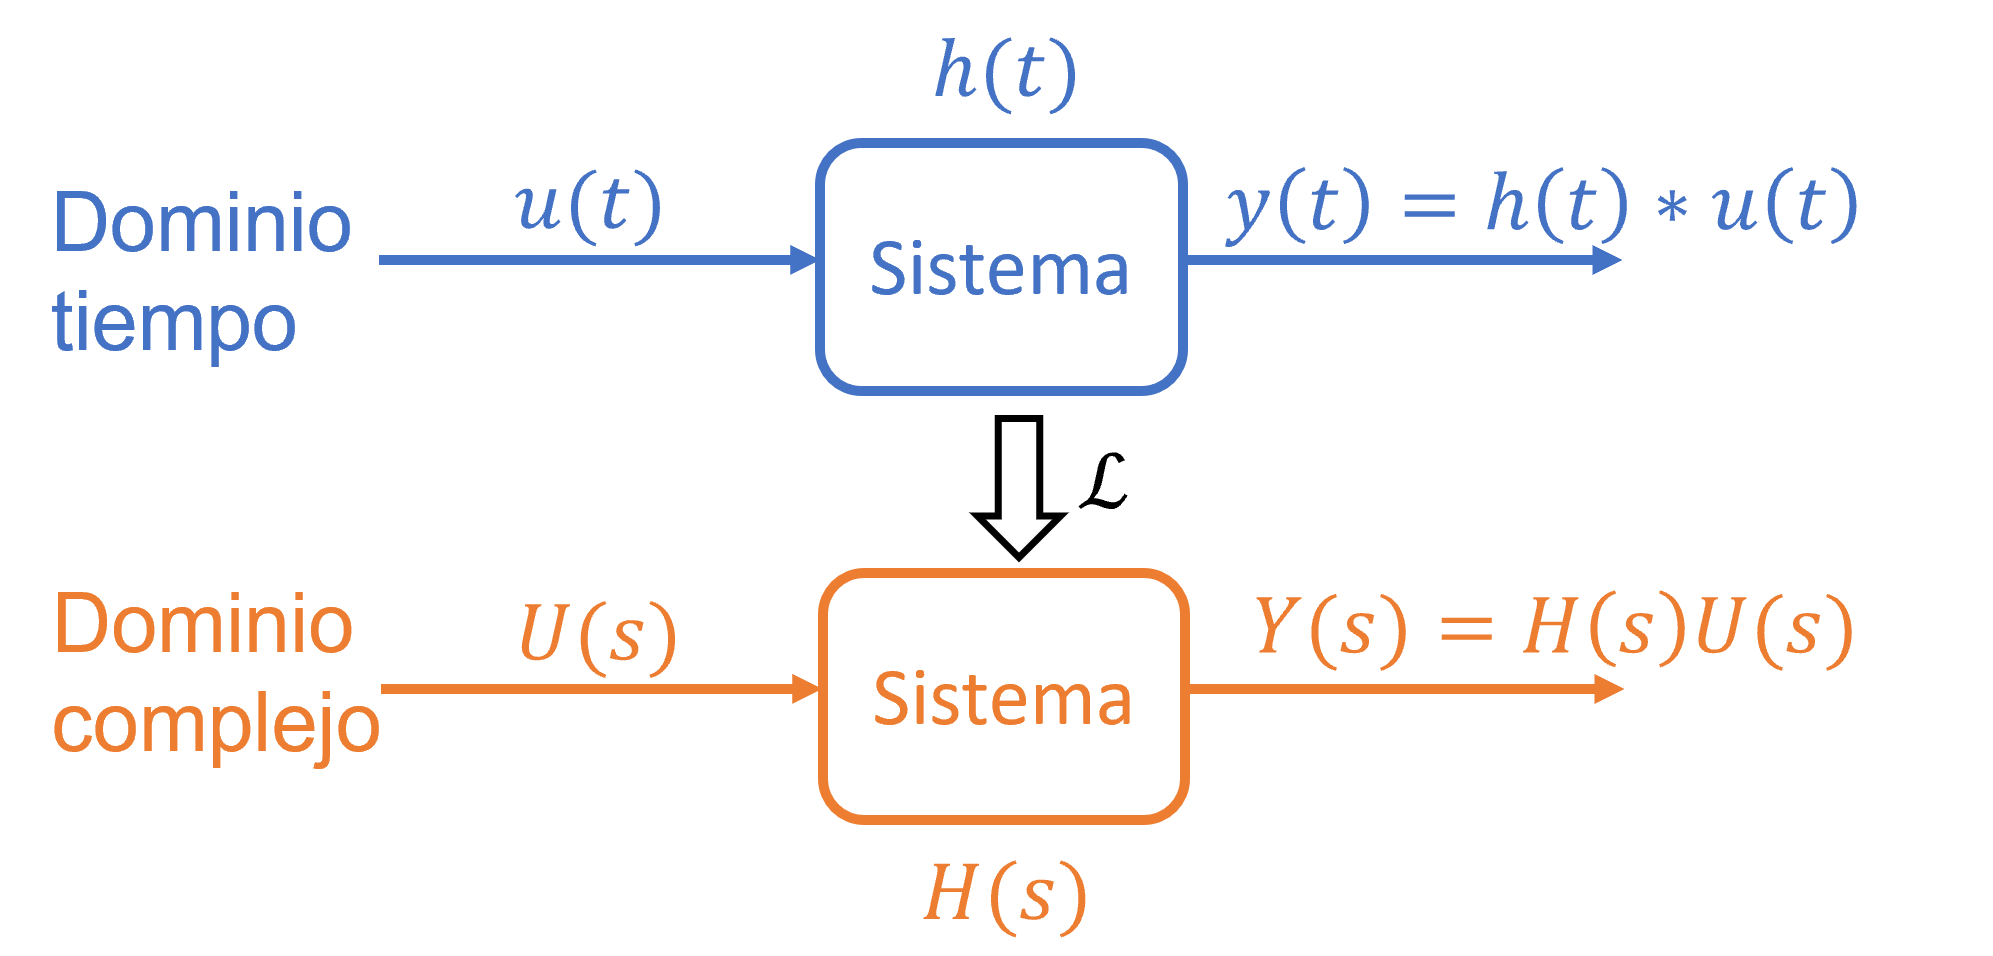
\includegraphics[scale=0.7]{TF.png}
\end{figure}

\underline{Definición}: $H(s)\in \mathbb{C}$ (función de transferencia)
\begin{align*}
    H(s)=\frac{\prod_{i=1}^m(s-z_i)}{\prod_{j=1}^n(s-p_j)}
\end{align*}
\begin{itemize}
    \item $z_i$: polos
    \item $p_j$: ceros
\end{itemize}

\underline{Definición}: $p_j \in \mathbb{C}$ (polos) son las raíces de la ecuación característica del sistema dinámico:
\begin{align*}
    \prod_{j=1}^n(s-p_j)=0
\end{align*}

\underline{Definición}: $z_i \in \mathbb{C}$ (ceros) son las raíces del polinomio del numerador:
\begin{align*}
    \prod_{i=1}^m(s-z_i)=0
\end{align*}

\underline{Importante}: La función de transferencia recopila \textcolor{red}{toda} la información del sistema dinámico en los coeficientes de los polinomios del numerador y denominador o equivalentemente con los polos y ceros.

\section{Plano complejo}
Para visualizar las propiedades dinámicas del sistema, vamos a trabajar en el plano complejo.

\begin{figure}[H]
\centering
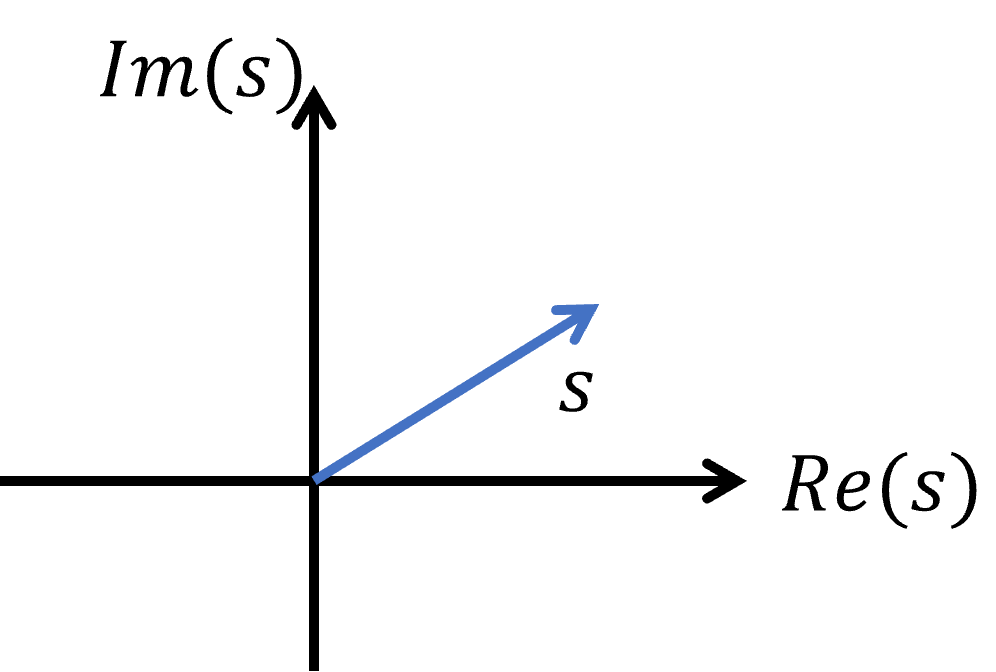
\includegraphics[scale=0.7]{plano_complejo.png}
\end{figure}

Los ceros $z_i$ y polos $p_j$ son puntos sobre el plano complejo
\begin{figure}[H]
\centering
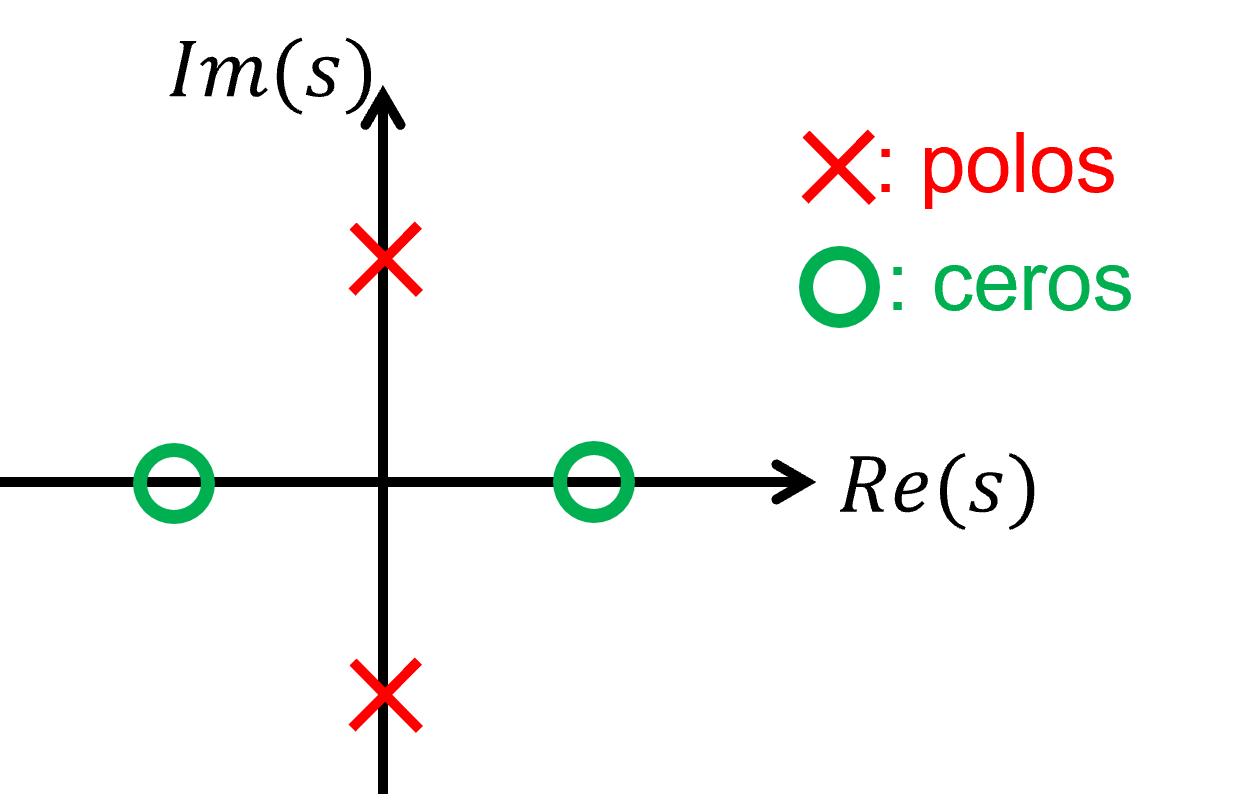
\includegraphics[scale=0.7]{polos_ceros.png}
\end{figure}

\newpage
$|H(s)|$ representa una ``superficie'' sobre el plano complejo
\begin{figure}[H]
\centering
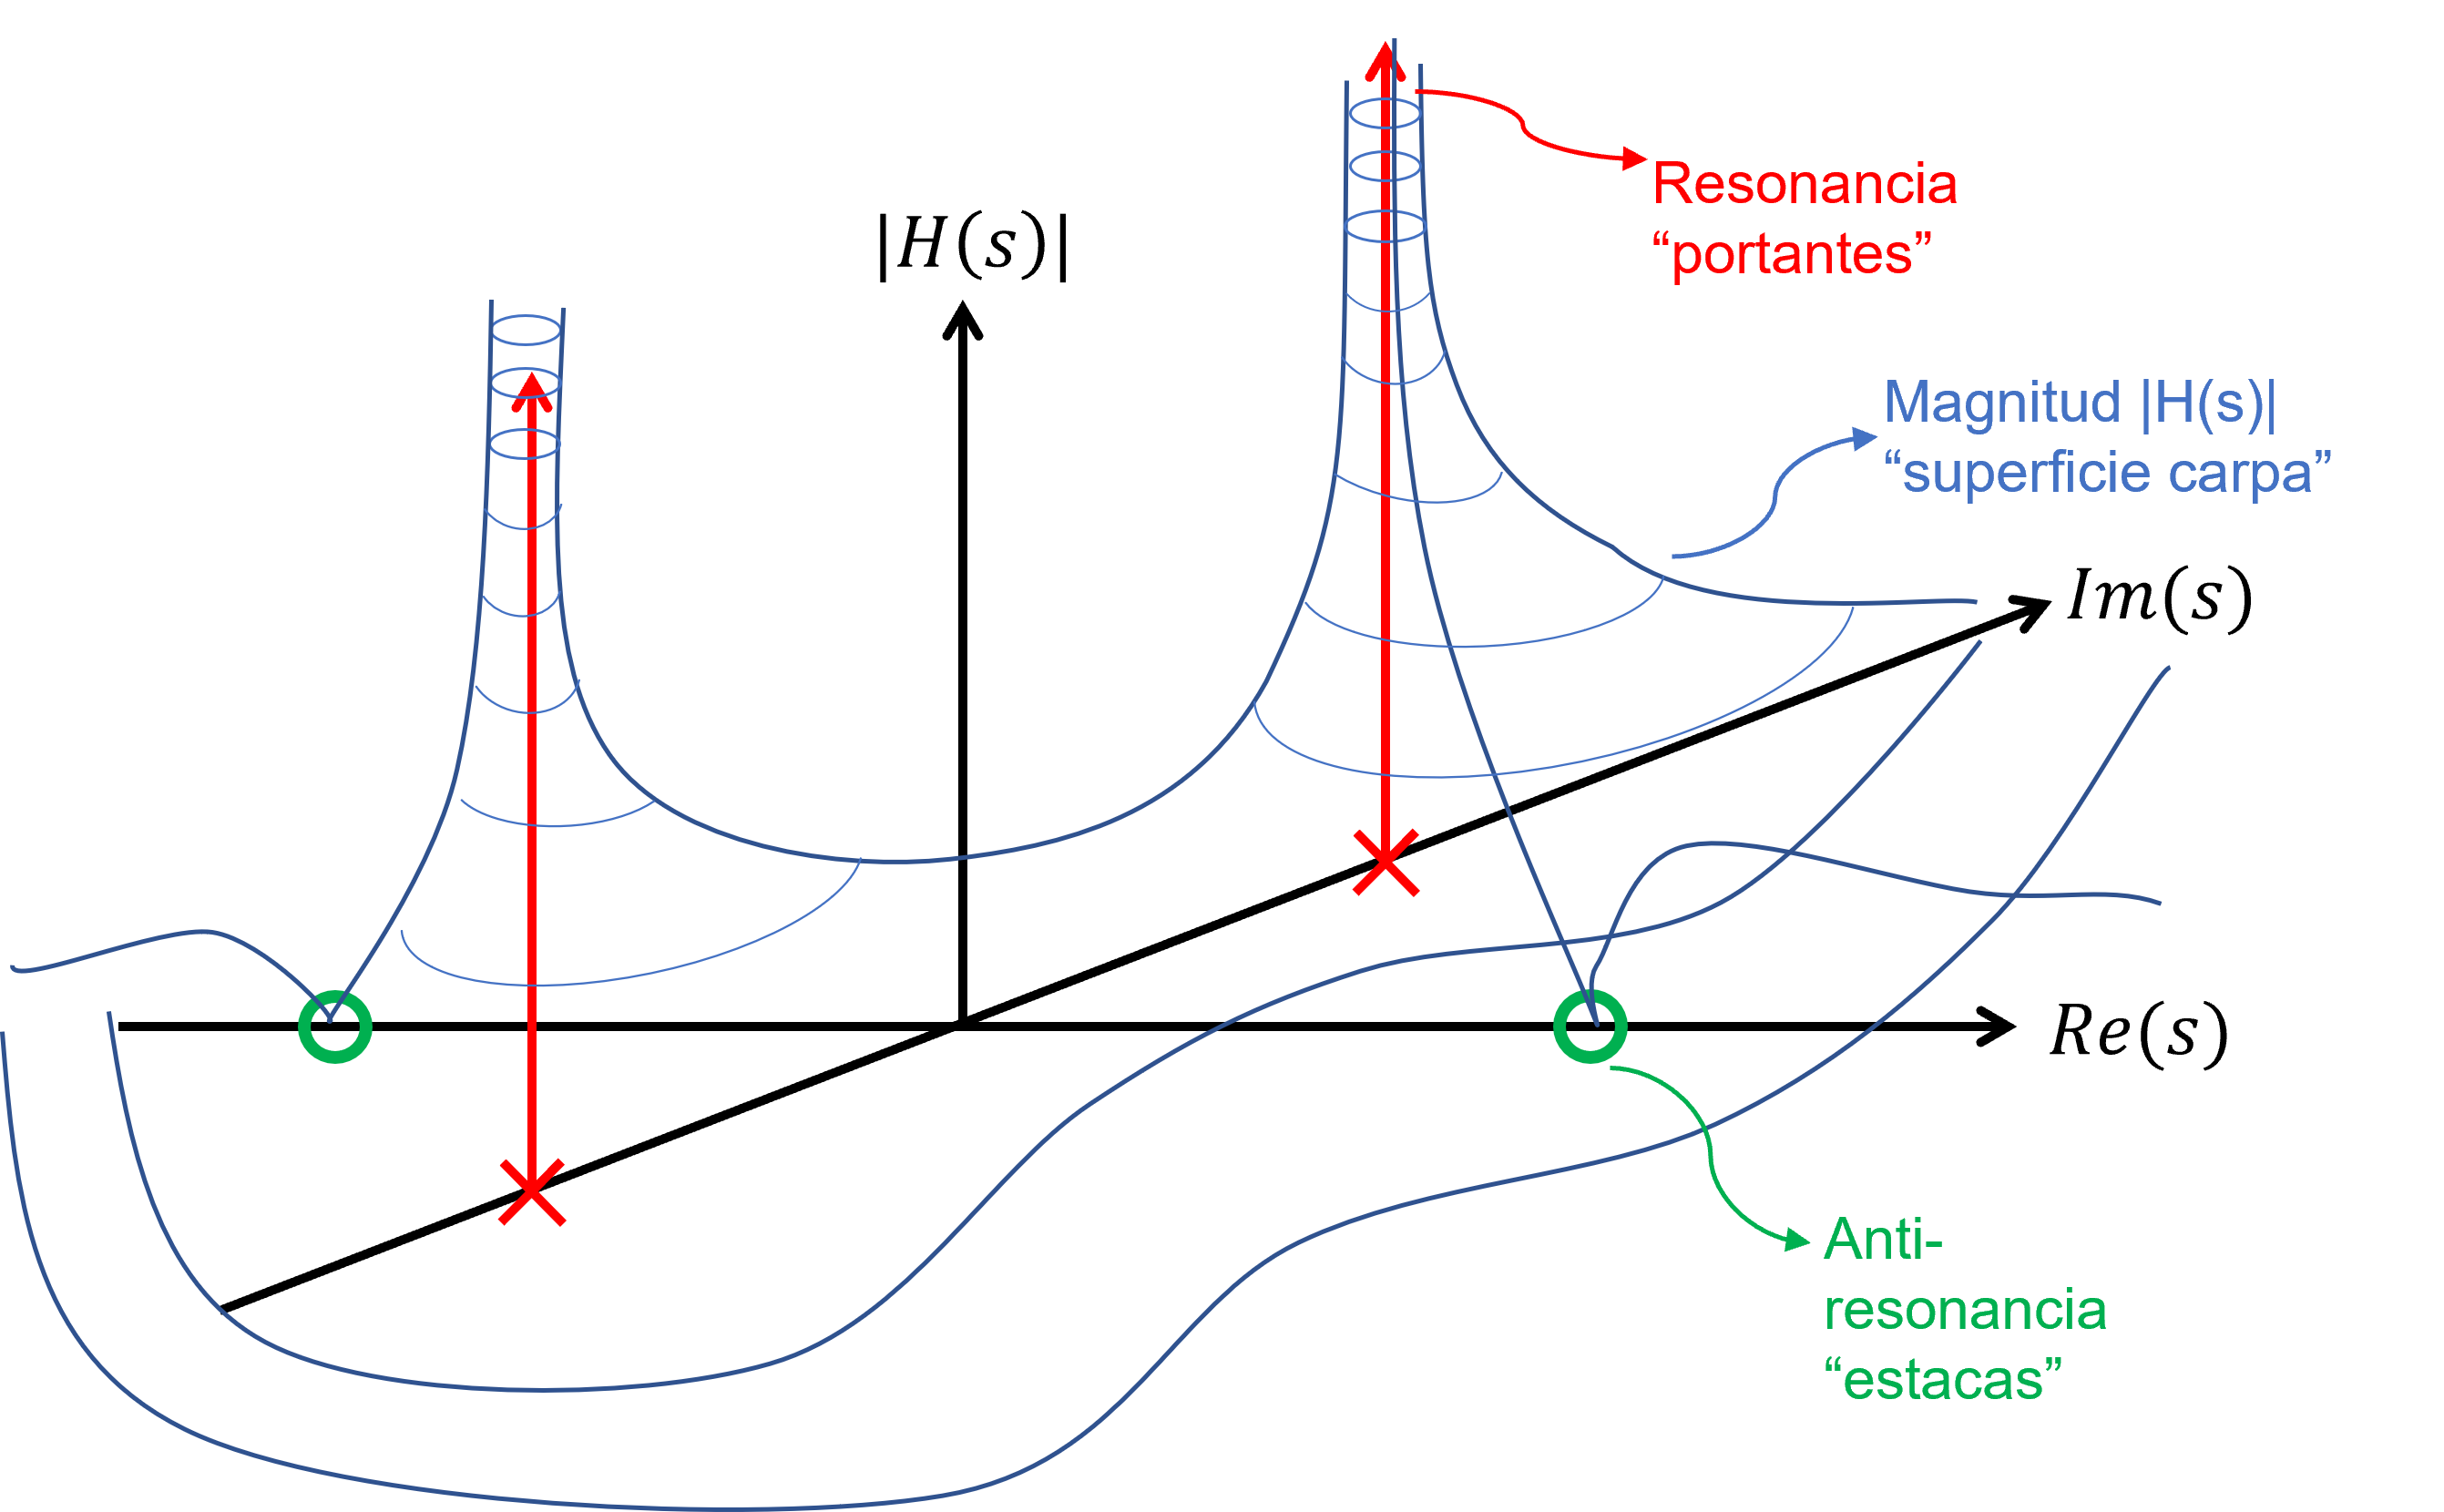
\includegraphics[scale=0.7]{magHs.png}
\end{figure}

\underline{Aparte}: Recordar que $H(s)$ corresponde a: $H(s)=\mathcal{L}\{h(t)\}$ ($h(t)$ es FRI), por ende, $h(t)=\mathcal{L}^{-1}\{H(s)\}$. Por lo tanto, los polos nos dan información del FRI.\\

Ejemplo: Si tenemos la siguiente función de transferencia $H(s)=\frac{1}{s-a}$, se puede obtener la FRI aplicando la inversa de la transformada de Laplace $h(t)=\mathcal{L}^{-1}\{H(s)\}=e^{at}$\\

\underline{Casos}:
\begin{itemize}
    \item[(i)] $a>0, ~a\in\mathbb{R}\Longrightarrow h(t)=e^{-|a|t}$
    \begin{figure}[H]
    \centering
    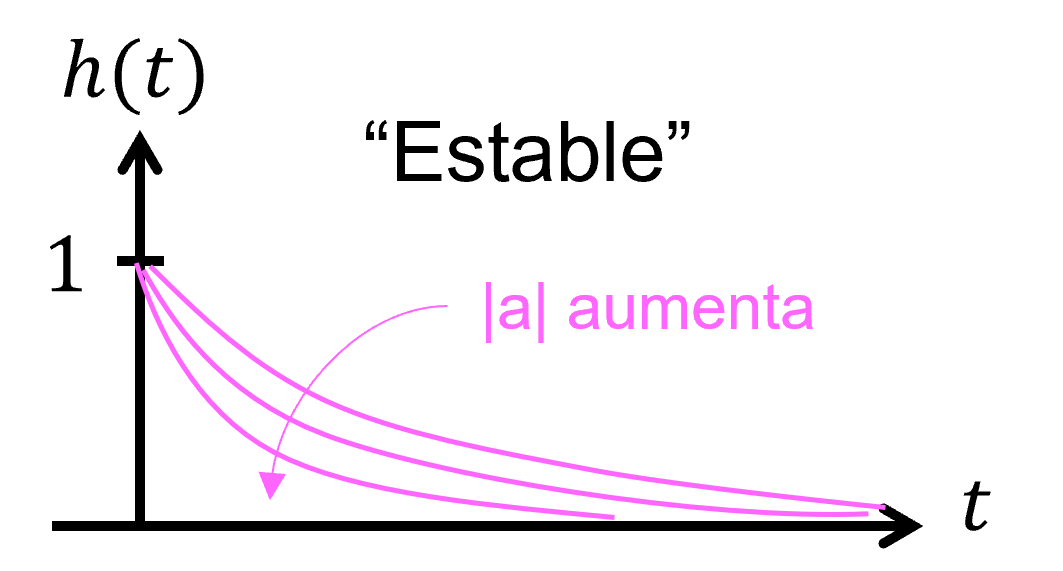
\includegraphics[scale=0.7]{caso1.png}
    \end{figure}
    \item[(ii)] $a=0, ~a\in\mathbb{R}\Longrightarrow h(t)=1$
    \begin{figure}[H]
    \centering
    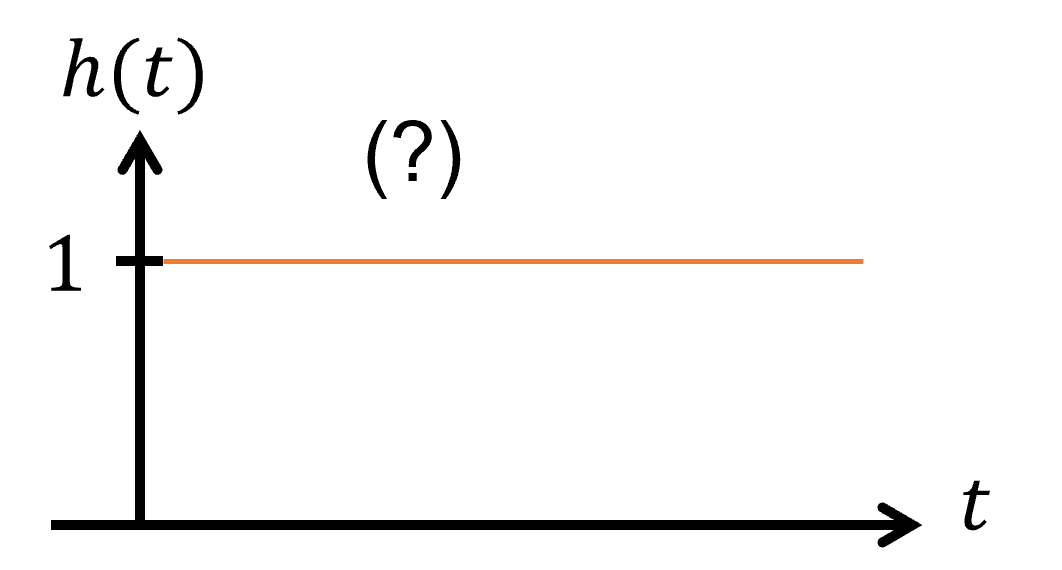
\includegraphics[scale=0.7]{caso2.png}
    \end{figure}
    \item[(iii)] $a<0, ~a\in\mathbb{R}\Longrightarrow h(t)=e^{|a|t}$
    \begin{figure}[H]
    \centering
    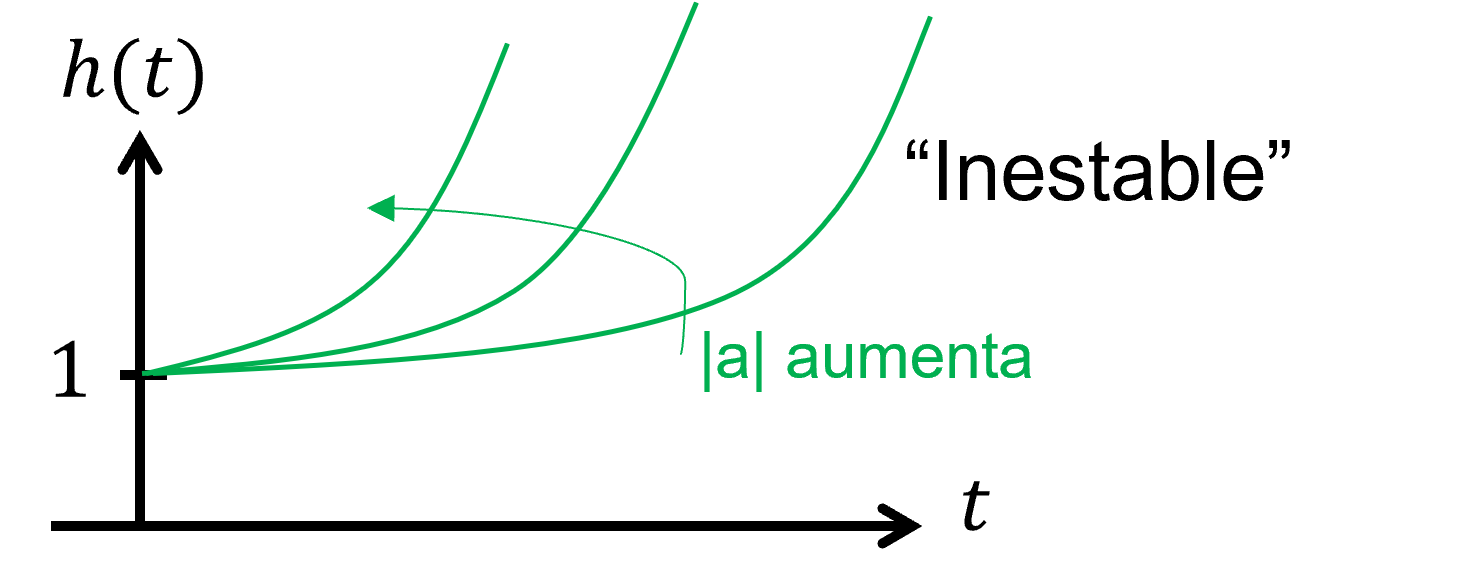
\includegraphics[scale=0.7]{caso3.png}
    \end{figure}
    \item[(iv)] $H(s)=\frac{1}{s^2+a^2}\Longrightarrow s_{1,2}=\pm \beta j \in \mathbb{C}$\\ \\
    $h(t)=\mathcal{L}^{-1}\{H(s)\}=\sin{(\beta t)}$\begin{figure}[h]
    \centering
    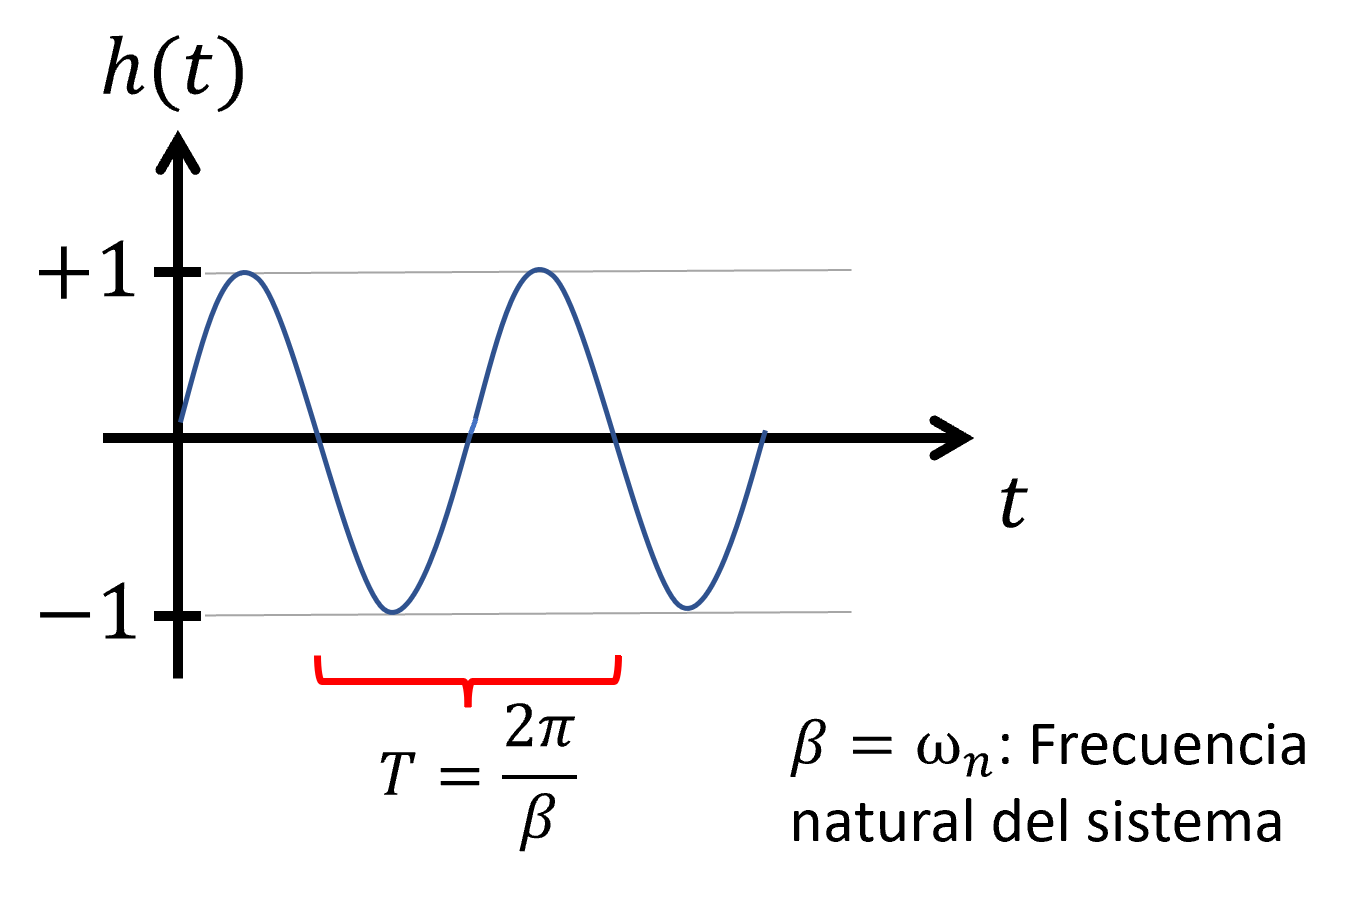
\includegraphics[scale=0.7]{caso4.png}
    \end{figure}
    
    \item[(v)] $a_{1,2}=\alpha\pm\beta j \in \mathbb{C}$ (polos conjugados)\\ \\
    \begin{align*}
        H(s) &= \frac{1}{(s-\alpha)^2+\beta^2} \longrightarrow \text{Raíces del denominador}\Rightarrow a_{1,2}\\
        h(t) &= \mathcal{L}^{-1}\{H(s)\} = e^{+\alpha t}\sin{(\beta t)}
    \end{align*}
    \begin{itemize}
        \item[(a)] $\alpha<0$ \\ \\
        $h(t) = e^{-|\alpha| t}\sin{(\beta t)}$
        \begin{figure}[h]
        \centering
        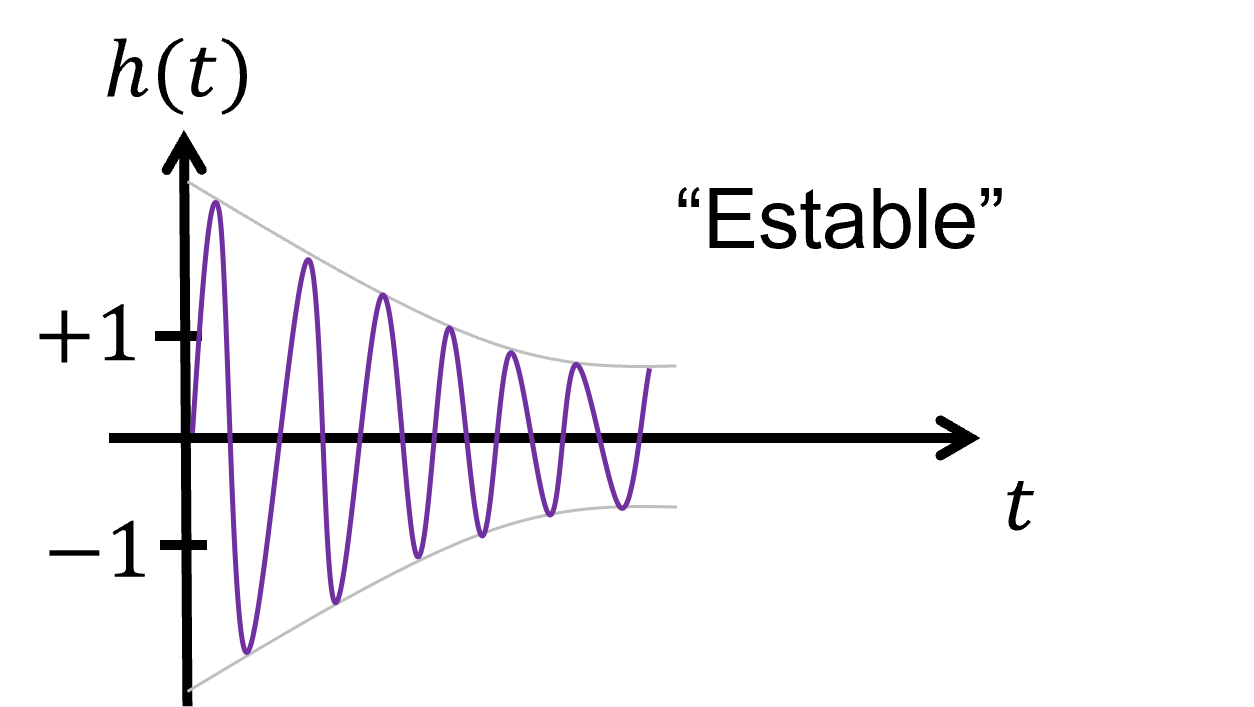
\includegraphics[scale=0.7]{caso5a.png}
        \end{figure}
        
        \item[(b)] $\alpha>0$\\ \\ 
        $h(t) = e^{+|\alpha| t}\sin{(\beta t)}$
        \begin{figure}[h]
        \centering
        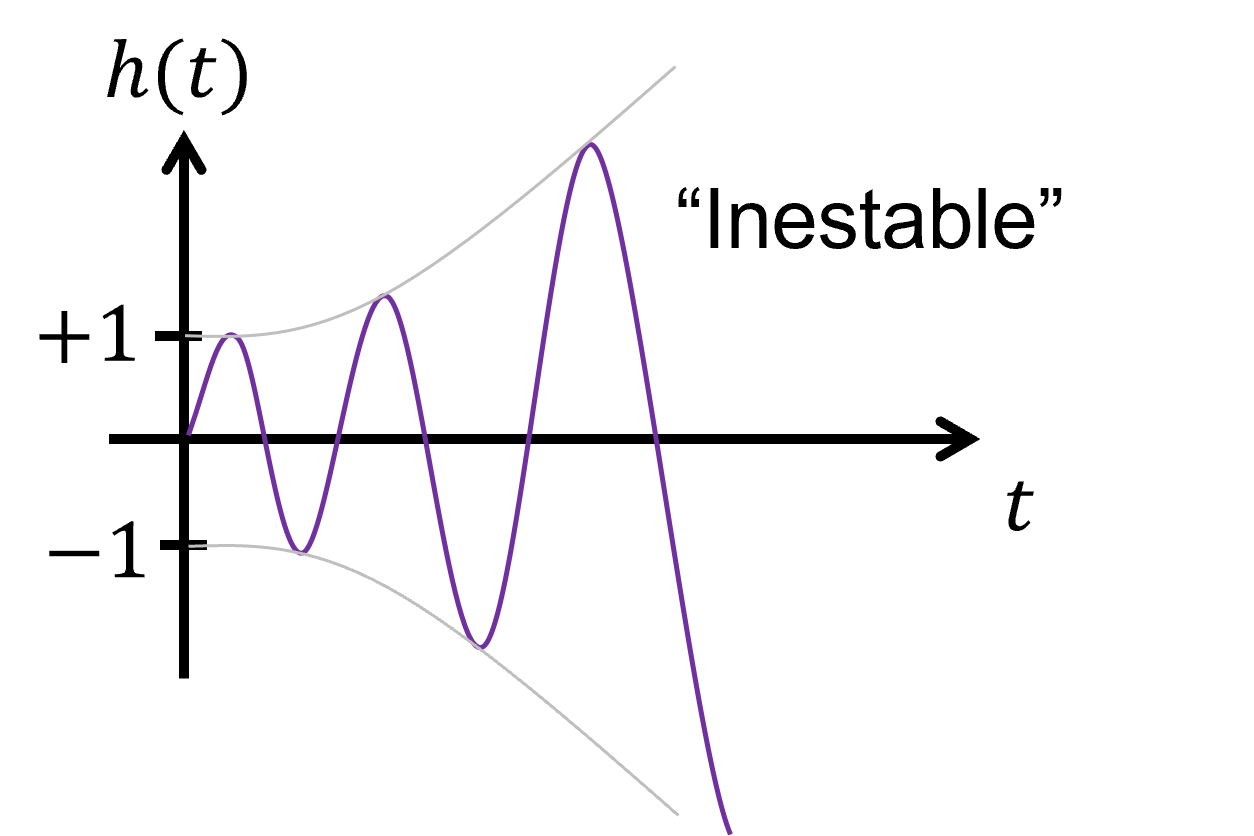
\includegraphics[scale=0.7]{caso5b.png}
        \end{figure}
        
        \item[(c)] $\alpha=0$\\ \\
        $h(t)=\sin{(\beta t)}\Longrightarrow$ volvemos al caso (iv).
    \end{itemize}
\end{itemize}

\underline{Volviendo al plano complejo}, podemos identificar el tipo de respuesta FRI del sistema solo con información de la posición de los polos:
\begin{figure}[H]
\centering
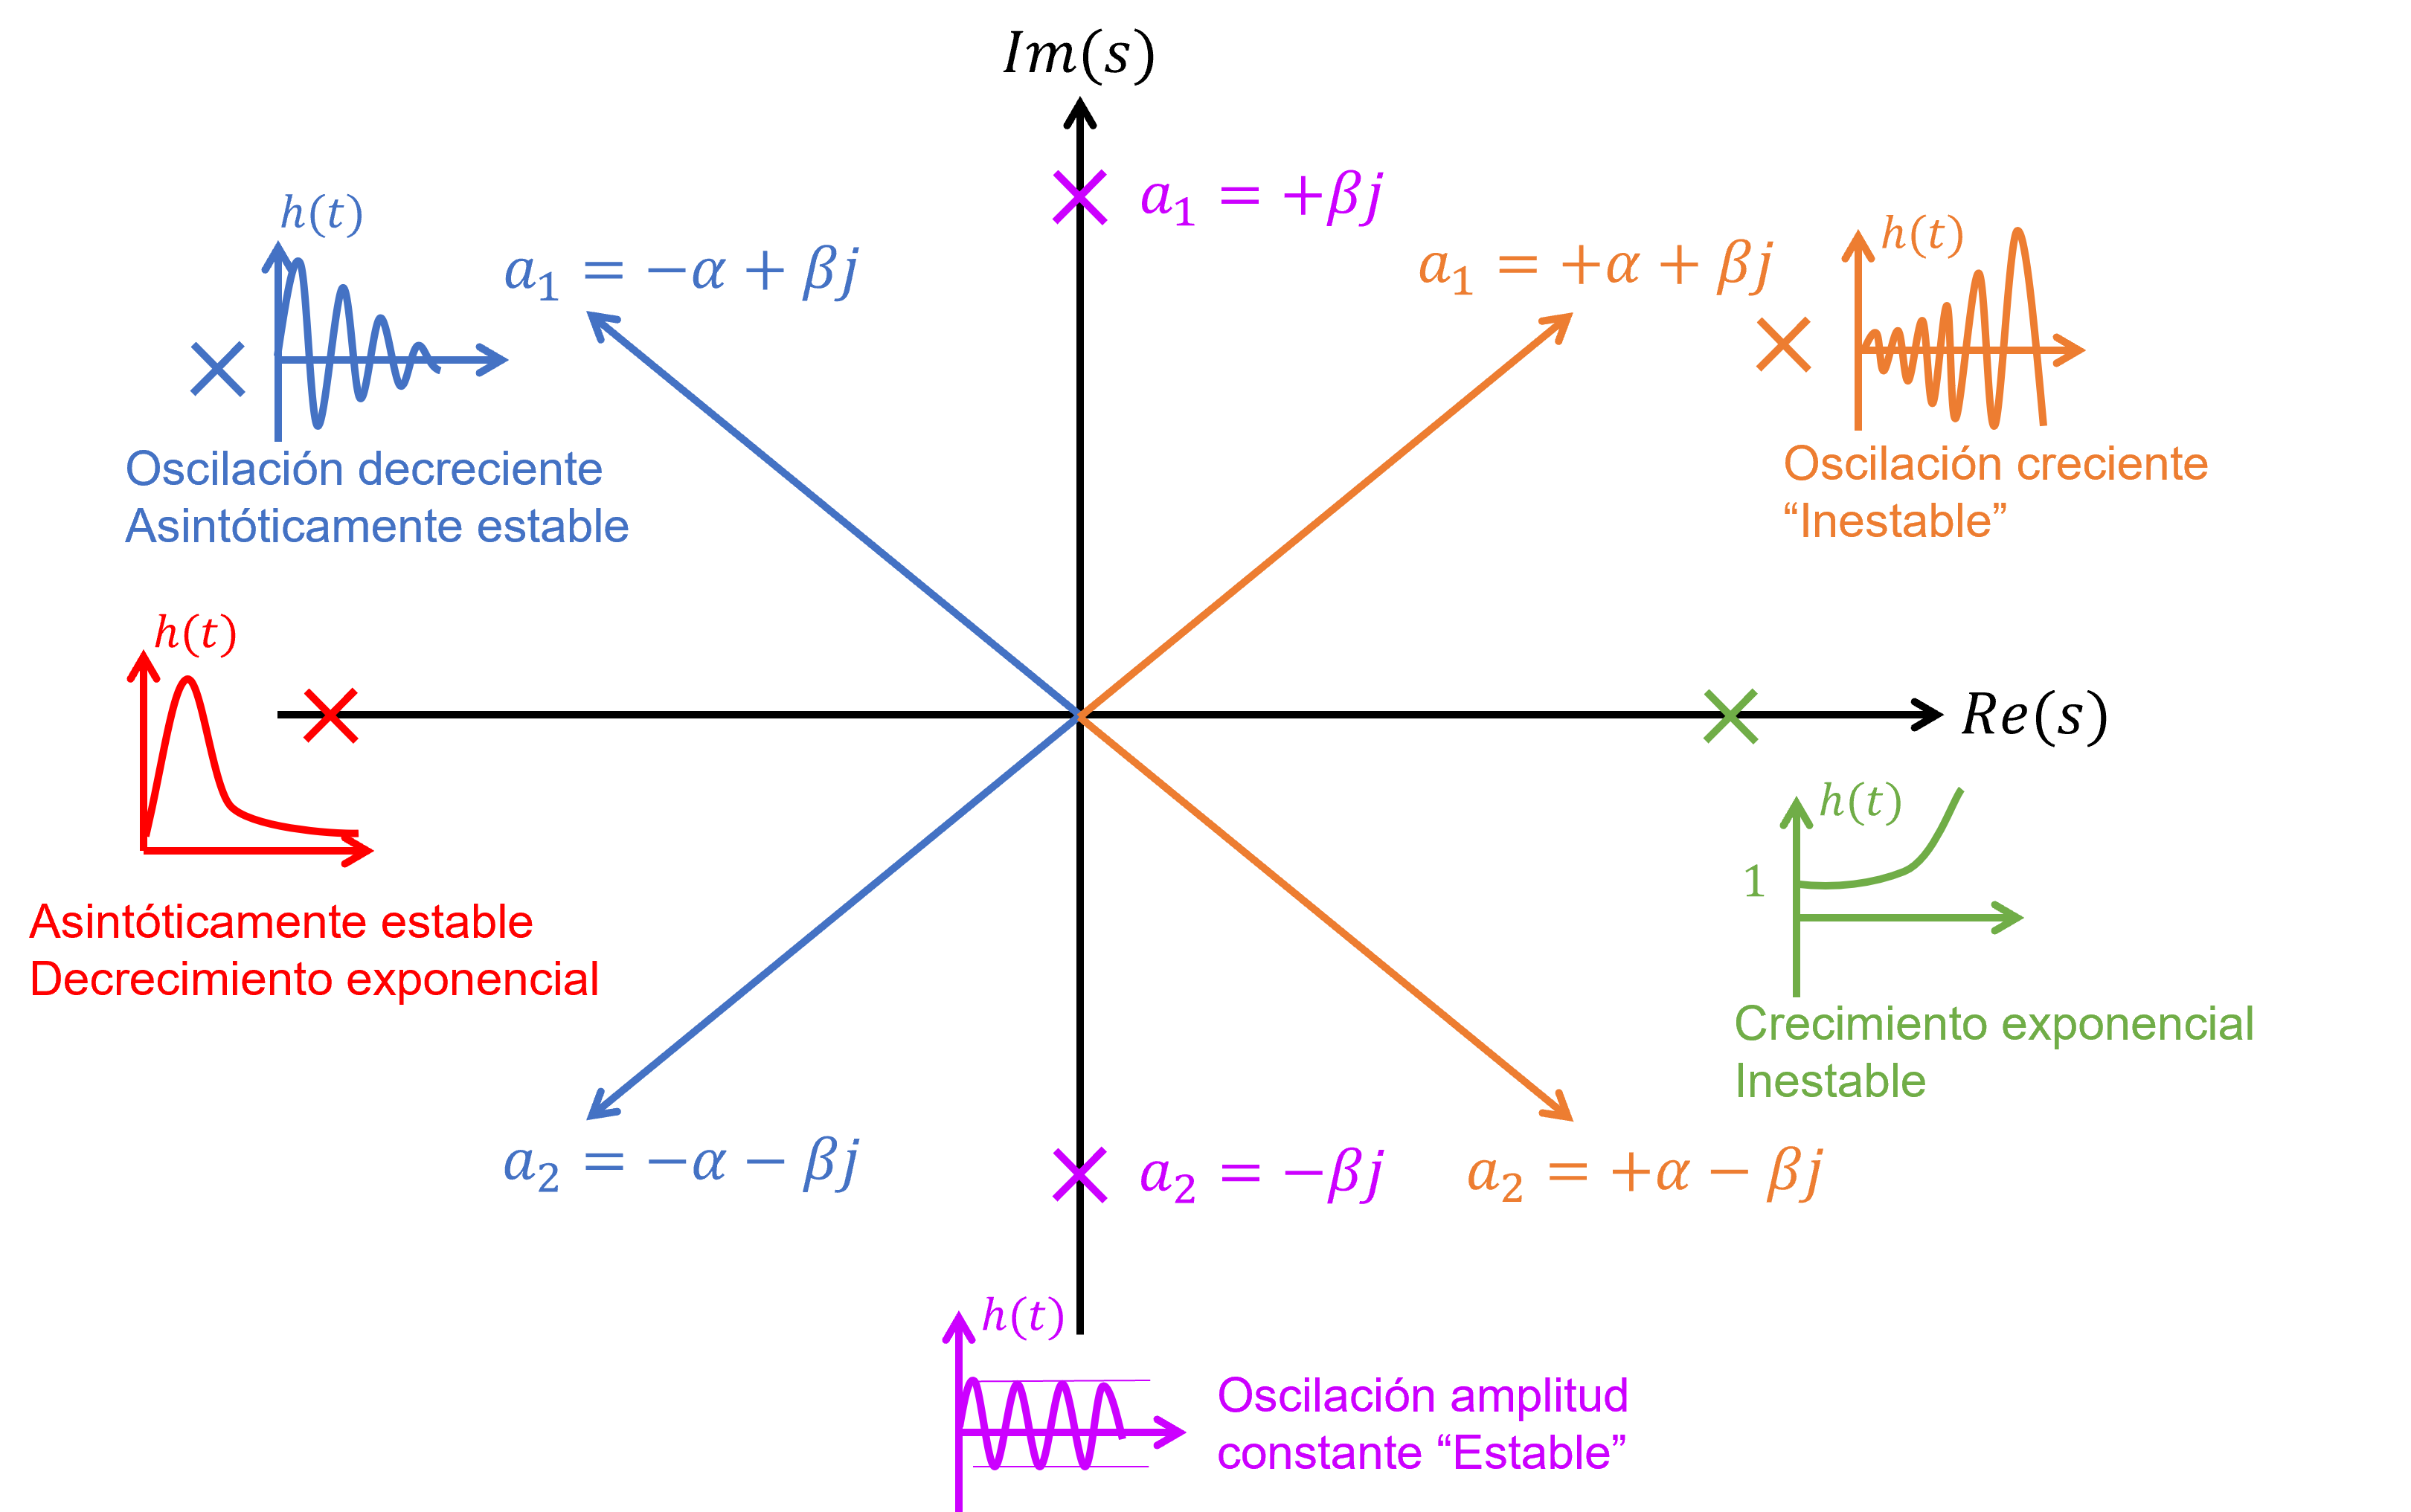
\includegraphics[scale=0.7]{Estabilidad1.png}
\end{figure}

\section{Estabilidad ``Bounded Input, Bounded Output'' (BIBO)}
\begin{figure}[H]
\centering
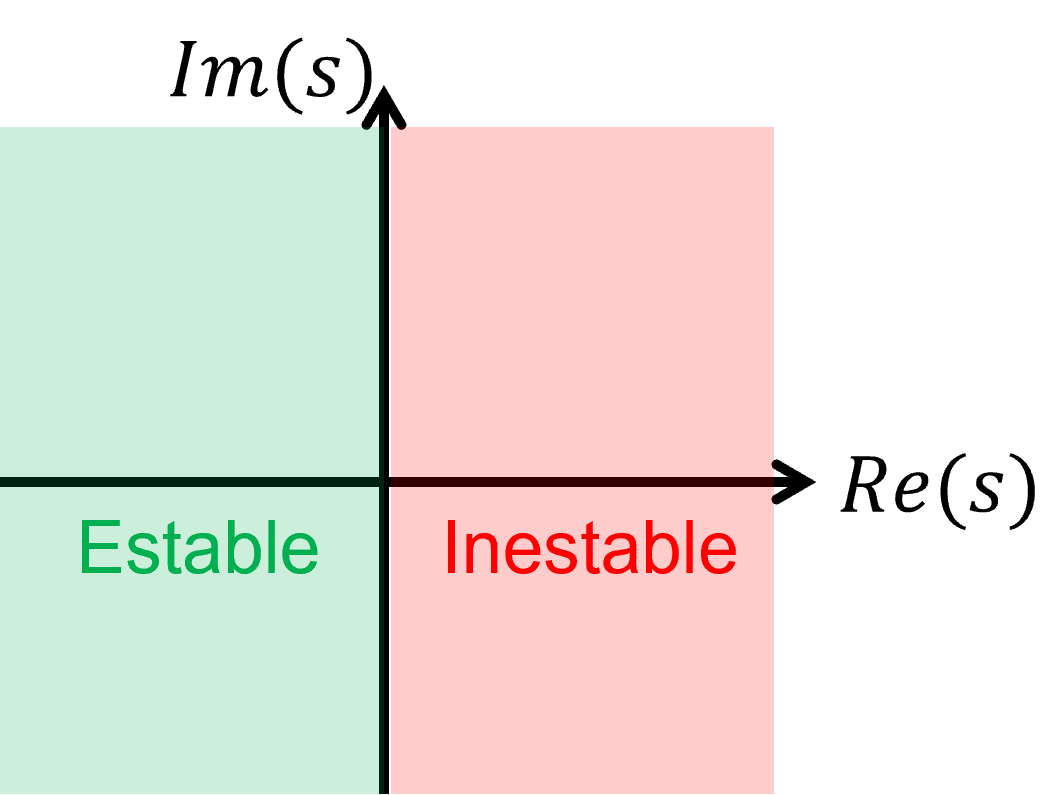
\includegraphics[scale=0.7]{BIBO.png}
\end{figure}
Un sistema es estable en el sentido BIBO, si y sólo si el sistema posee todos sus polos a la izquierda del plano complejo. Dicho de otra forma: $p_i=\alpha_i\pm\beta_i j$
\begin{itemize}
    \item \textcolor{ForestGreen}{El sistema es estable BIBO ssi $Re(p_i)=\alpha_i<0$}
    \item \textcolor{red}{Si el sistema posee al menos un polo cuyo $Re(p_i)=\alpha_i>0$, entonces el sistema es inestable}
\end{itemize}

\section{Implementación utilizando Matlab/Simulink}

En matlab se puede trabajar con sistemas dinámicos utilizando \emph{variables tipo sistema}. Estas variables se puede crear si se cuenta con la información de alguna de las representaciones vistas anteriormente. \\

Para State-Space se requieren las matrices $\tenq{A}$, $\tenq{B}$, $\tenq{C}$, $\tenq{D} \Longrightarrow$ matrices de tipo ``double'' \\

\par Para construir un sistema desde representación espacio-estado, se utiliza el siguiente comando:
\begin{minted}[]{matlab}
>> sys = ss(As, Bs, Cs, Ds); % Variable tipo sistema 
\end{minted}

Para representar utilizando la función de transferencia se requiere conocer los coeficientes de los polinomios del numerador y denominador de la función de transferencia:

\begin{align*}
    H(s)=\frac{b_ms^m+b_{m-1}s^{m-1}+...+b_1s+b_0}{s^n+a_{n-1}s^{n-1}+...+a_1s+a_0}
\end{align*}

\par Se utiliza el siguiente comando para construir la variable tipo sistema:
\begin{minted}[]{matlab}
>> sys = tf(num,den); % Variable tipo sistema 
\end{minted}

Donde:
\begin{align*}
    \text{num} = [b_m, b_{m-1}, ... , b_1, b_0]\\
    \text{den} = [1, a_{n-1}, ... , a_1, a_0]
\end{align*}

Ejemplo de coeficientes para sistema 1GDL:
\begin{align*}
    \text{num} = [1/m]\\
    \text{den} = [1, c/m, k/m]
\end{align*}

También, se pueden generar conociendo los polos, ceros y la ganancia del sistema:
\begin{align*}
    \text{TF: }~H(s)= k\frac{\prod_{i=1}^m(s-z_i)}{\prod_{j=1}^n(s-p_j)}
\end{align*} 
\begin{align*}
    \text{zeros} &= [z_m, z_{m-1}, ..., z_2, z_1]\\
    \text{poles} &= [p_n, p_{n-1},..., p_2, p_1]\\
    \text{gain} &= k
\end{align*} 

\par Ocupando los polos, ceros y ganancia, también se puede generar una variable tipo sistema:
\begin{minted}[]{matlab}
>> sys = zpk(ceros, polos, gain); 
\end{minted}

\underline{Matlab: Control System Toolbox}\\

El toolbox \emph{Control System} de matlab permite también extraer información y simular las variables de tipo sistema.

\begin{itemize}
    \item Valores y vectores propios del sistema:
\begin{minted}[]{matlab}
>> eig(sys)
>> eig(As)
\end{minted}
\item Polos del sistema, frecuencias naturales y razones de amortiguamiento:
\begin{minted}[]{matlab}
>> damp(sys)
>> damp(As)
\end{minted}
\item Posición de ``ceros'' y ``polos'' en el plano complejo:
\begin{minted}[]{matlab}
>> pzmap(sys)
\end{minted}
\item Gráfico magnitud y fase vs frecuencia del sistema
\begin{minted}[]{matlab}
>> bode(sys)
>> bodeplot(sys)
\end{minted}
\item Ganancia del sistema
\begin{minted}[]{matlab}
>> dcgain(sys) %% DC: direct current (caso estático)
\end{minted}

\item Análisis: respuesta a impulso y a escalón
\begin{minted}[]{matlab}
>> impulse(sys)
>> step(sys)
\end{minted}
\end{itemize}

\chapter{Teoría de Sistemas Lineales}

\section{Matriz de transición de estados}
\subsection{Para LTI autónomo}
Sea un sistema LTI autónomo, es decir, sin entrada $u(t)$. Su solución $\tend{x}(t)$ se puede obtener utilizando transformación de Laplace:

\begin{align*}
    &\phantom{\Longrightarrow} \tend{\dot{x}}(t) =\tenq{A}\tend{x}(t)~/\mathcal{L}\{\cdot\}\\
    &\Longrightarrow s\tend{X}(s)-\tend{x_0} = \tenq{A}\tend{X}(s)\\
    &\Longrightarrow (s\tenq{I}-\tenq{A})\tend{X}(s) =\tend{x_0}\\
    &\Longrightarrow \tend{X}(s) = (s\tenq{I}-\tenq{A})^{-1}\tend{x_0}~/\mathcal{L}^{-1}\{\cdot\}\\
    &\Longrightarrow \tend{x}(t) = e^{\tenq{A}t}\tend{x_0}
\end{align*}

definiendo $\tenq{\phi}(t) = e^{\tenq{A}t}$ como la \emph{matriz de transición de estados}, la respuesta de los estados del sistema queda determinada por la siguiente expresión:

\begin{align*}
    \Longrightarrow \tend{x}(t) = \tenq{\phi}(t)\tend{x_0}
\end{align*}

Notar que $\tenq{\phi}(t)$ es una matriz que varía en función del tiempo.

\noindent \underline{Aparte}: Para entender qué significa $e^{\tenq{A}t}$ hay que recordar la Expansión de Taylor de una exponencial.\\

\noindent \underline{Definición}: Sea $f(t)$ una función suave y continua, su \emph{Expansión de Taylor} en torno a $t = \alpha$ es la siguiente:
\begin{align*}
    f(t) = f(\alpha)+\frac{\dot{f}(\alpha)}{1!}(t-\alpha)+\frac{\ddot{f}(\alpha)}{2!}(t-\alpha)^2+... = \sum_{n=0}^{\infty}{\frac{(t - \alpha)^n}{n!}\frac{d^n}{dt^n}f(t = \alpha)}   
\end{align*}
aplicando la expansión en una función exponencial en en torno a $\alpha = 0$:
\begin{align*}
    e^{at} = 1+at+\frac{1}{2!}a^2t^2+\frac{1}{3!}a^3t^3+... 
\end{align*}

La Expansión de Taylor de una exponencial también converge en torno a $\alpha = 0$ cuando se utiliza una matriz $\tenq{A}$ cuadrada. Por lo tanto, $\tenq{\phi}(t) = e^{\tenq{A}t}$ se puede calcular utilizando la siguiente serie:
\begin{align*}
    \tenq{\phi}(t) = e^{\tenq{A}t} = \tenq{I}+\tenq{A}t+\frac{1}{2!}\tenq{A}^2t^2+\frac{1}{3!}\tenq{A}^3t^3+...
\end{align*}

Notar que la expansión de Taylor de $\tenq{\phi}(t) = e^{\tenq{A}t}$ es una serie infinita. La serie finita se obtiene con el \emph{Teorema de Cayley-Hamilton} que se encuentra más adelante.

\underline{Nota}: $\tenq{\phi}(t)$ satisface la ecuación de estado:

\begin{align*}
    \Longrightarrow \tend{x}(t) &= \tenq{\phi}(t)\tend{x_0} = \left[\tenq{I}+\tenq{A}t+\frac{1}{2!}\tenq{A}^2t^2+...\right]\tend{x_0}\\
    \Longrightarrow \tend{\dot{x}}(t) &= \left[\tenq{A}+\frac{2}{2!}\tenq{A}^2t+...\right]\tend{x_0} =  \tenq{A}\left[\tenq{I}+\tenq{A}t+\frac{1}{2!}\tenq{A}^2t^2+...\right]\tend{x_0}\\
    \Longrightarrow \tend{\dot{x}}(t) &= \tenq{A}\tenq{\phi}(t)\tend{x_0}=\tenq{A}\tend{x}(t) \quad \text{(Ecuación de Estado)}
\end{align*}

\subsection{Para LTI no autónomo}
Si tenemos un sistema LTI no autónomo (es decir, con entrada u), la respuesta se encuentra de forma análoga:
\begin{align*}
    &\phantom{\Longrightarrow} \tend{\dot{x}}(t) = \tenq{A}\tend{x}(t)+\tenq{B}\tend{u}(t)\\
    &\Longrightarrow s\tend{X}-\tend{x_0} = \tenq{A}\tend{X}+\tenq{B}\tend{U}\\
    &\Longrightarrow (s\tenq{I}-\tenq{A})\tend{X} = \tend{x_0}+\tenq{B}\tend{U}\\
    &\Longrightarrow \tend{X}(s) = (s\tenq{I}-\tenq{A})^{-1} \tend{x_0}+(s\tenq{I}-\tenq{A})^{-1} \tenq{B}]tend{U}(s)\\
    &\Longrightarrow \tend{x}(t) = \tenq{\phi}(t)\tend{x_0}+\left[ \tenq{\phi}(t)\tenq{B} \right] \ast u(t)\\
    &\Longrightarrow \tend{x}(t) = \tenq{\phi}(t)\tend{x_0}+\int_0^t\tenq{\phi}(t-\tau)\tenq{B}\tend{U}(\tau)d\tau
\end{align*}

Notar que:
\begin{align*}
    \tenq{\phi}(t-\tau)&=e^{\tenq{A}(t-\tau)}\\
    &=e^{\tenq{A}t}\cdot e^{-\tenq{A}\tau}\\ 
    &=\tenq{\phi}(t)\tenq{\phi}(-\tau)
\end{align*} 

\noindent \underline{Aparte:} Sobre las propiedades de $\tenq{A}$, del problema de valores propios:
$$\tenq{A}\tend{v}=\lambda\tend{v}$$
donde $\tend{v}$ y $\lambda$ son el vector y valor propio asociado.
\begin{align*}
    \Longrightarrow \tenq{\phi}(t)\tend{v} &= \left[\tenq{I}+\tenq{A}t+\frac{1}{2!}\tenq{A}^2t^2+...\right]\tend{v}\\
    &= \tend{v}+\tenq{A}\tend{v}t+\frac{1}{2!}\tenq{A}^2\tend{v}t^2+... \\
    &= \tend{v}+\lambda\tend{v}t+\frac{1}{2!}\lambda^2\tend{v}t^2+... \\
    &= \left[ 1+\lambda t+\frac{\lambda^2}{2!}+\frac{\lambda^3}{3!}t^3 + ...\right]\tend{v}
\end{align*}
Si $\tend{x_0}=\tend{v}$, entonces $\tend{x}(t)=\tenq{\phi}(t)\tend{v}$\\

\noindent \underline{Aparte}: $\phi(t)$ una serie infinita ssi $\text{Re}(\lambda)<0$. Entonces el sistema LTI es estable.
\begin{align*}
    \lim_{t \to \infty} \phi(t)<\infty     
\end{align*}

\noindent \underline{Definición}: Una matriz $\tenq{A}$ se dice que es \textbf{Hurwitz} ssi los valores propios de $\tenq{A}$ tienen una parte real estrictamente negativa.


\section{Teorema de Cayley-Hamilton}
\underline{Teorema}: Sea una matriz $A\in\mathbb{R}^{n\times n}$, cuya ecuación característica $\Delta(\tenq{A}) = 0$ está dada por el siguiente polinomio de orden $n$:
\begin{align*}
    \Delta(\tenq{A})=\text{det}(s\tenq{I}-\tenq{A})=s^n+\alpha_{n-1}s^{n-1}+...+\alpha_1s+\alpha_0=0
\end{align*}
donde $\alpha_i\in\mathbb{R}$, $i\in [0,n-1]$, son los coeficientes del polinomio característico de $\tenq{A}$. Entonces, el teorema establece que la matriz $\tenq{A}$ también satisface la ecuación característica:
\begin{align*}
    \Delta (\tenq{A})=\tenq{A}^n+\alpha_{n-1}\tenq{A}^{n-1}+...+\alpha_1\tenq{A}+\alpha_0\tenq{I}=\tenq{0}
\end{align*}

Del teorema, podemos despejar $\tenq{A}^n$:
\begin{align*}
    \tenq{A}^n &= -\left[\alpha_{n-1}\tenq{A}^{n-1}+...+\alpha_1\tenq{A}+\alpha_0\tenq{I} \right]
\end{align*}

El poder de una matriz se escribe como una serie polinomial de orden igual al exponente del poder.\\

\par $\Longrightarrow$ Este resultado es útil para evaluar la matriz de transición $\phi(t)$
\begin{align*}
    \tenq{\phi(t)}=e^{\tenq{A}t}=\sum_{i=0}^\infty \beta_i(t)\tenq{A}^i \overset{\text{(C-H)}}{=} \sum_{i=0}^{n-1}\gamma_i(t)\tenq{A}^i
\end{align*}

\underline{Nota}: Este resultado es útil para evaluar $\phi(t)$ como una serie finita en términos de $A^i$.


\section{Equilibrio y Estabilidad}
\subsection{Plano de Fase}
El plano de Fase o diagrama de fase, es una representación gráfica de las trayectorias de un sistema dinámico en el tiempo, es decir, se puede observar como varían los estados en función del tiempo y entender mejor el comportamiento del sistema. También permite observar gráficamente la estabilidad. \\

Ejemplo: Considere el siguiente sistema dinámico LTI Autónomo de un grado de libertad.
\begin{figure}[H]
\centering
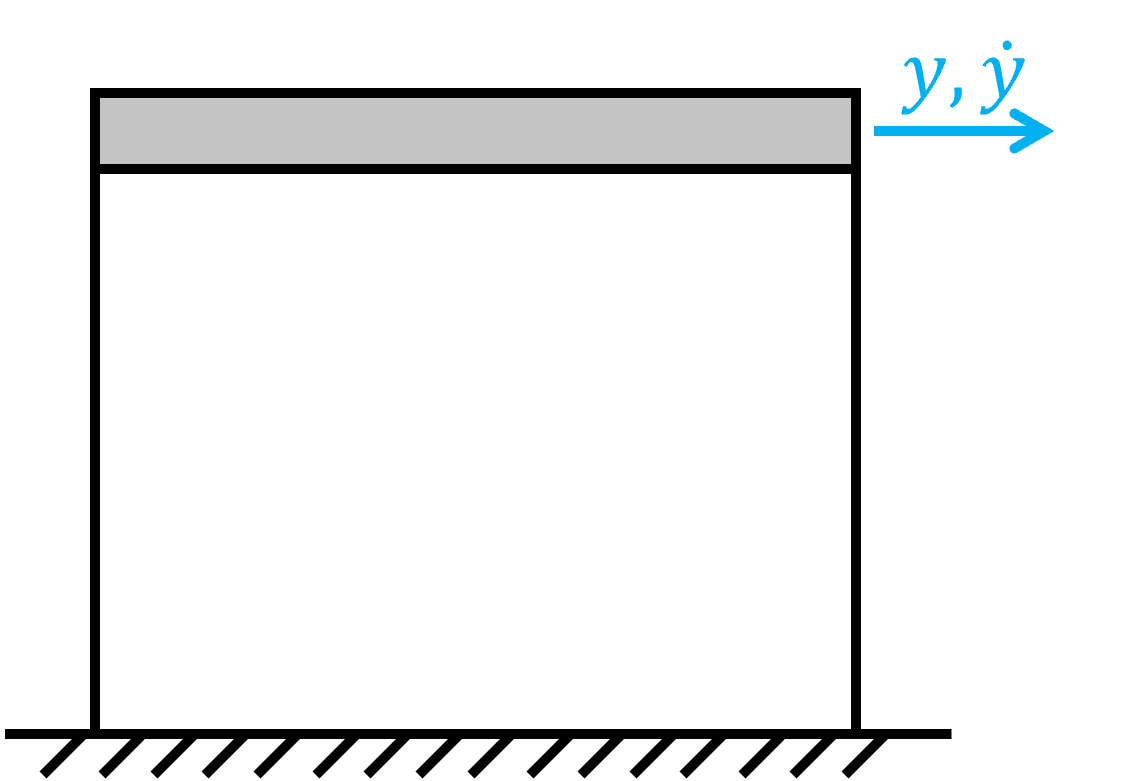
\includegraphics[scale=0.7]{Figuras/leccion11.png}
\end{figure}

\begin{align*}
    \Longrightarrow \tend{\dot{x}}(t) =\tenq{A}\tend{x}(t)
\end{align*}
donde $\tend{x}(t)=\begin{bmatrix} y(t)\\ \dot{y}(t) \end{bmatrix}$, con condiciones iniciales $y_0$, $\dot{y}_0$, se puede generar el siguiente diagrama de fase en el que se observa cómo varían los estados en el tiempo.
\begin{figure}[H]
\centering
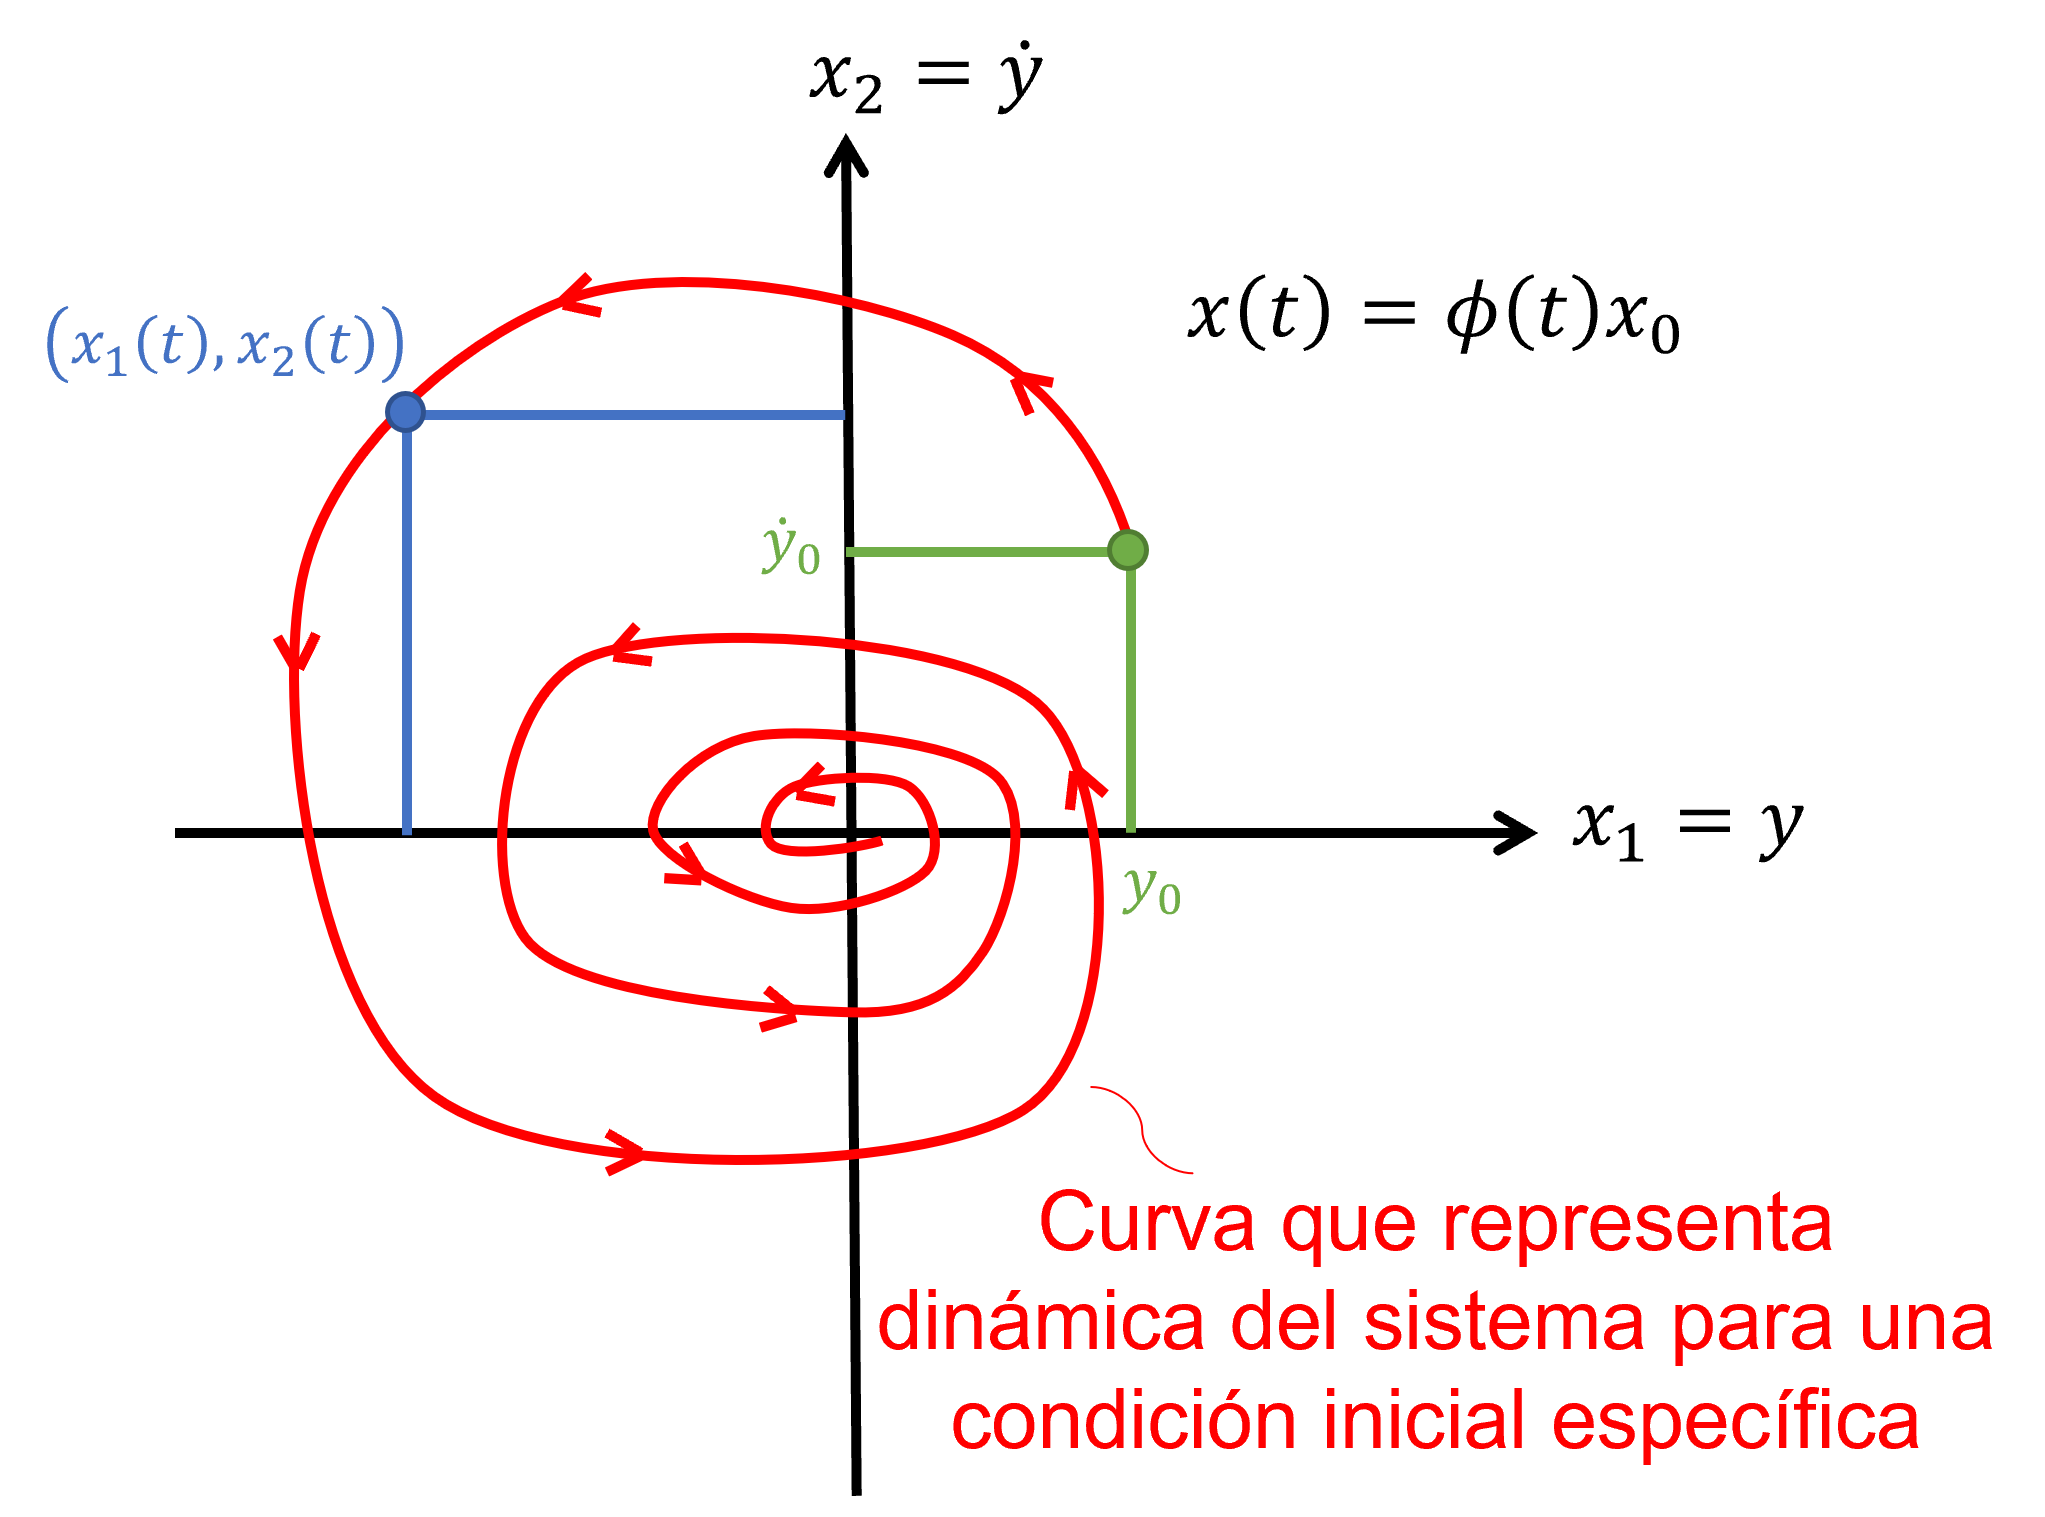
\includegraphics[scale=0.7]{Figuras/plano_de_fase.png}
\end{figure}
Notar que el diagrama de fase puede ser para cualquier vector de estados y no únicamente para dos estados como en este ejemplo.

\begin{figure}[H]
\centering
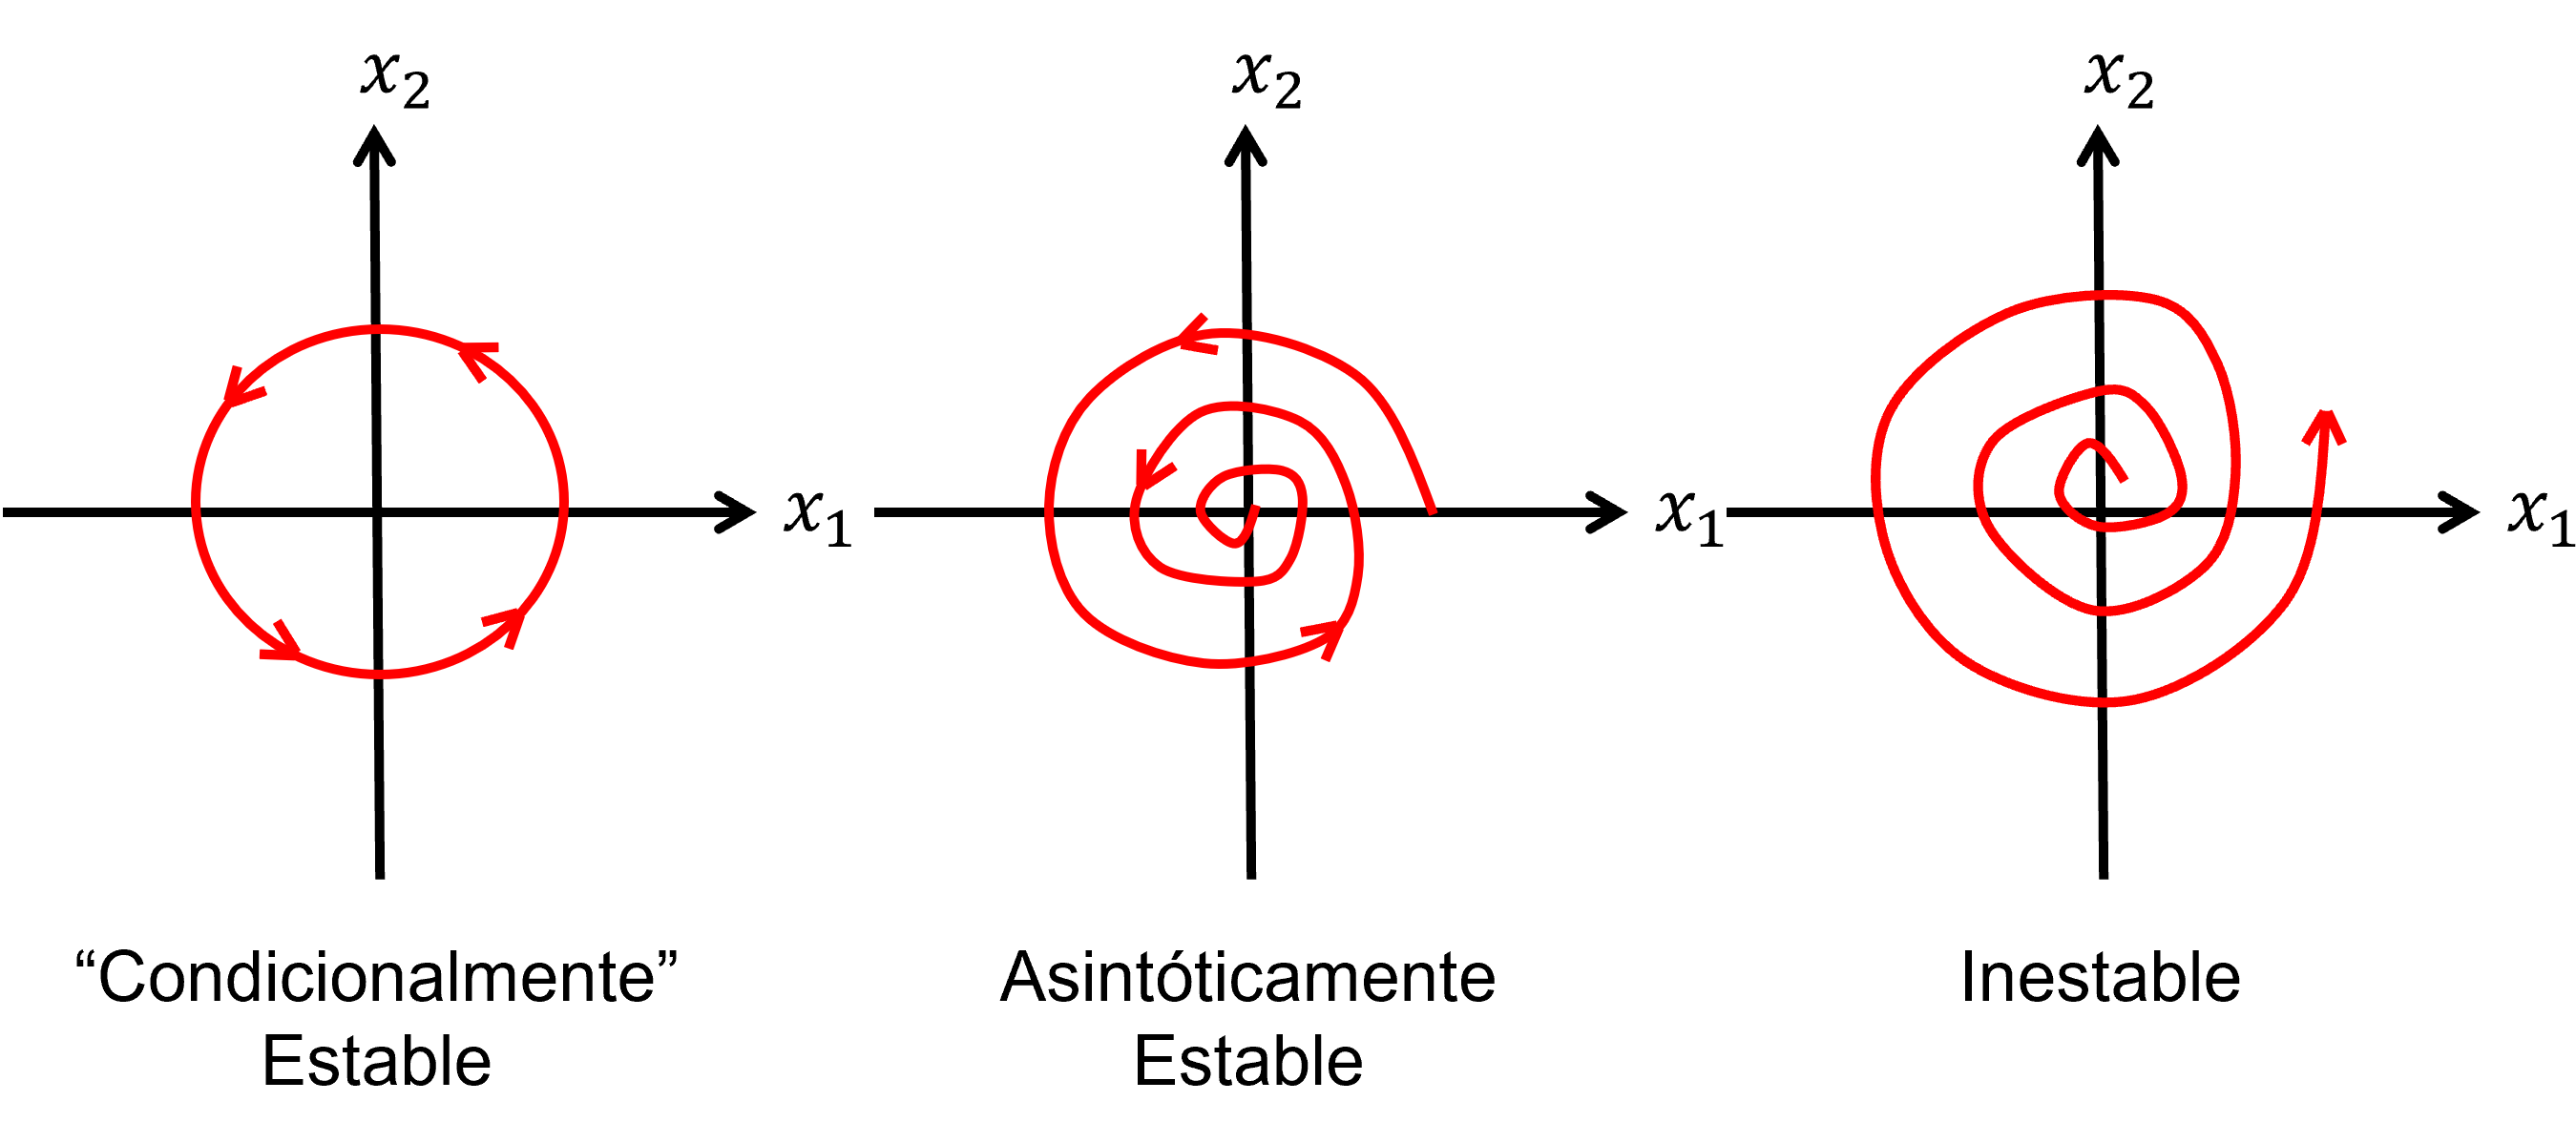
\includegraphics[scale=0.7]{Figuras/plano_de_fase.png_2.png}
\end{figure}

\subsection{Equilibrio}
Sea el sistema dinámico LTI en representación espacio-estado:
$$\tend{\dot{x}}=\tenq{A}\tend{x}+\tenq{B}\tend{u} $$

\noindent encontraremos una expresión para encontrar el estado en equilibrio $\tend{x_e}$. \\

\underline{Definición}: El equilibrio del sistema está dado por la condición de que $\tend{x}$ no cambia en el tiempo:
\begin{align*}
    \tend{\dot{x}} = \tend{0}
\end{align*}
Entonces, despejando el estado de equilibrio $\tend{x_e}$ desde el sistema LTI:
\begin{align*}
    &\Longrightarrow \tend{0}=\tenq{A}\tend{x_e}+\tenq{B}\tend{u_e} \\
    &\Longrightarrow \tend{x_e}=-\tenq{A}^{-1}\tenq{B}\tend{u_e} \Longrightarrow \text{ Estados de Equilibrio Estático}
\end{align*}

\noindent donde $\tend{x_e}$ es el vector de estado en equilibrio y $\tend{u_e}$ es el vector de entrada en el equilibrio, ambos constantes. \\

\underline{Notas}
\begin{itemize}
    \item Notar que si: $\tend{u_e}=\tend{0}\Longrightarrow\tend{x_e}=\tend{0}$.
    \item Los sistemas lineales presentan sólo un estado de equilibrio $\tend{x_e}$.
    \item No confundir: los estados de equilibrio $\tend{x_e}$ no son necesariamente \emph{estables}.
\end{itemize}

\subsection{Estabilidad de Lyapunov}
Sea un sistema dinámico LTI y autónomo: $\dot{x}=Ax$, $x(0) = x_0$ y $x_e$ un punto de equilibrio del sistema. Vamos a definir la estabilidad respecto a un punto de equilibrio.\\
\par \underline{Definición}: $x_e$ es estable en el sentido de Lyapunov si para cualquier $\varepsilon >0$ existe un $\delta >0$ tal que:
$$||x_0-x_e||<\delta\Longrightarrow ||x(t)-x_e||<\varepsilon, \quad \forall t>0$$
\begin{figure}[H]
\centering
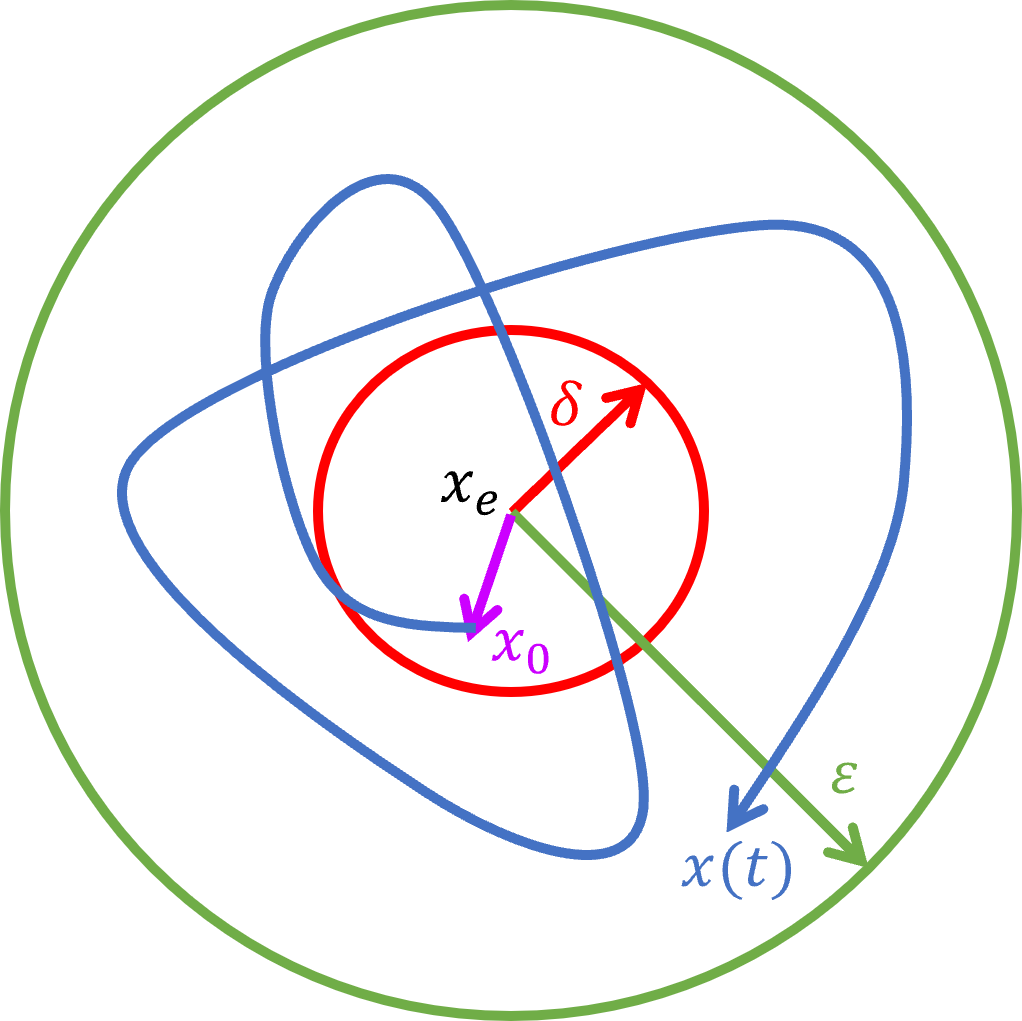
\includegraphics[scale=0.7]{Figuras/Lyapunov.png}
\end{figure}
* Mínima restricción que podemos imponer para satisfacer estabilidad.

\subsubsection{Definición Estabilidad Asintótica}
$x_e$ es asintóticamente estable si existe $\delta>0$ tal que:
\begin{itemize}
    \item $||x_0-x_e||<\delta$
    \item $x_e$ es estable en el sentido de Lyapunov
    \item $\lim_{t\to\infty}x(t)=x_e$
\end{itemize}
\begin{figure}[H]
\centering
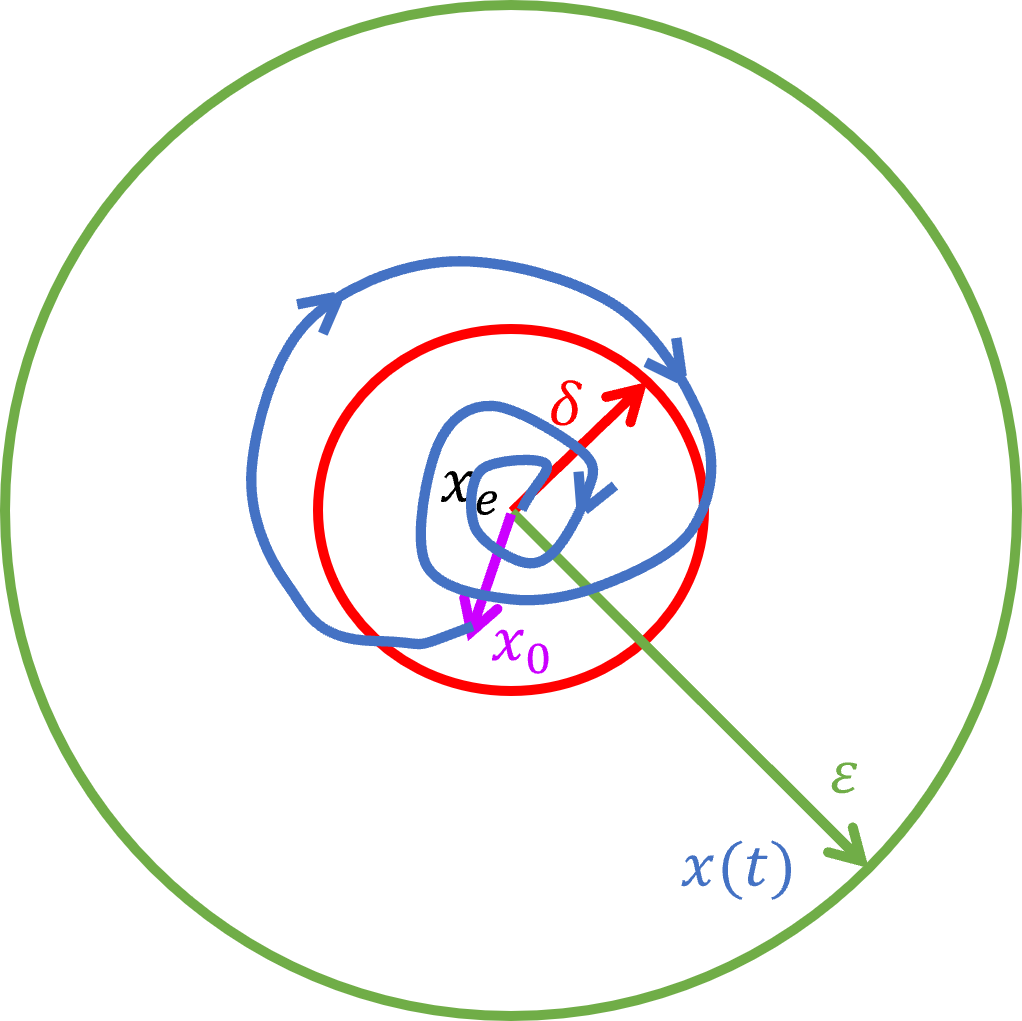
\includegraphics[scale=0.7]{Figuras/asintotica.png}
\end{figure}

\subsubsection{Definición Estabilidad Asintótica Global}
$x_e$ es estable asintótica global ssi es asintóticamente estable para $\delta \to \infty$.

\begin{table}[H]
    \centering
    \begin{tabular}{c|c|c|c|}
                & \raisebox{-\totalheight}{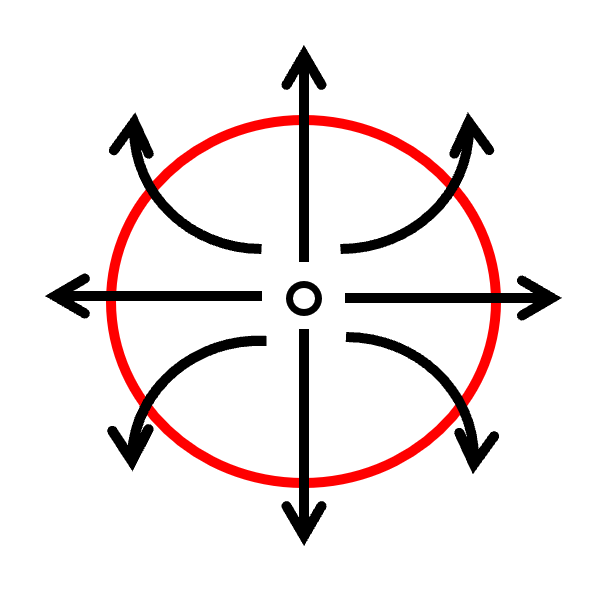
\includegraphics[scale=0.5]{Figuras/global1.png}} & \raisebox{-\totalheight}{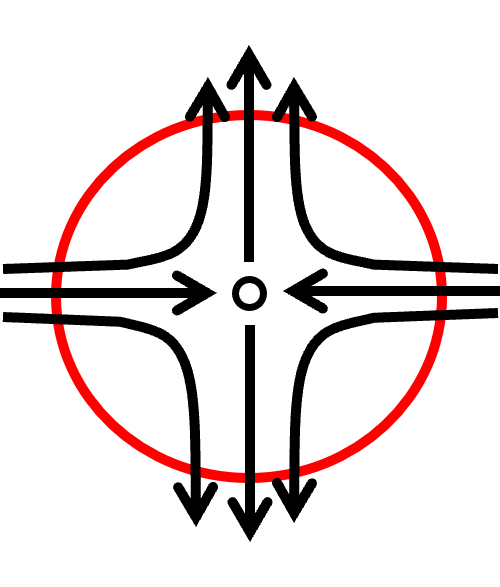
\includegraphics[scale=0.5]{Figuras/global2.png}} & \raisebox{-\totalheight}{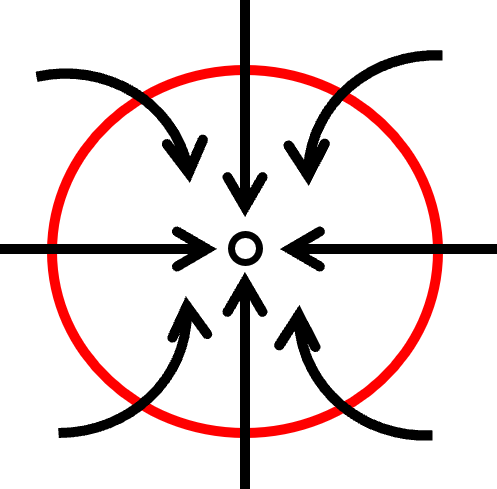
\includegraphics[scale=0.5]{Figuras/global3.png}}\\ \hline
         Estable & \xmark & \xmark & \cmark\\
         Asint. Est. & \xmark & \xmark &\cmark \\
         Goblal Asint. Est. & \xmark & \xmark & \textbf{???}
    \end{tabular}
\end{table}


\subsubsection{Límites de Estabilidad para sistemas LTI}
Sea el sistema LTI autónomo $\dot{x}(t)=Ax(t)$, cuya solución es $x(t)=\phi(t)x_0$ y $x_e$ un estado de equilibrio. Se requiere analizar la estabilidad en el sentido de Lyapunov. Por lo cual hay que analizar las normas $||x(t) - x_e||$ y $||x_0 - x_e||$ \\

\par Suponiendo que $\phi(t)$ es finita, es decir, $||\phi(t)||=||e^{At}||\leq\beta<\infty$. Se tiene que la siguiente diferencia de vectores de estados:
\begin{align*}
    x(t)-x_e &= \phi(t)x_0-x_e\\
    &= \phi(t)x_0-\phi(t)x_e\\
    &= \phi(t)[x_0-x_e]
\end{align*}

Para este sistema, notar que si $x_0 = x_e$, entonces $x(t)=x_e$, es decir, si el estado inicial es un estado de equilibrio (por ejemplo, el reposo) y si no existen exitaciones, entonces los estado $x(t)$  se mantendrán constantes e igual a al estado de equilibrio $x_e$, para $\phi(t)x_e=x_e$.\\

Entonces, extrayendo la norma de la expresión anterior:
\begin{align*}
    ||x(t)-x_e||=||\phi(t)[x_0-x_e]||\leq||\phi(t)||\cdot||x_0-x_e||
\end{align*}
Luego, si $||x_0 - x_e||<\delta$
\begin{align*}
    &\Longrightarrow ||x(t)-x_e||\leq ||\phi(t)|| \delta
\end{align*}
Si definimos $||\phi(t)||\delta = \varepsilon$:
\begin{align*}
    &\Longrightarrow ||x(t) - x_e|| \leq \varepsilon
\end{align*}

Por lo tanto, si $\phi(t)$ es finito, implica que $x_e$ es estable en el sentido de Lyapunov. 
$\phi(t)$ es finito si y solo si $A$ es Hurwitz:
\begin{align*}
    \text{Re}\left(\text{eig}(A)\right)<0\Longrightarrow \text{Estabilidad}
\end{align*}

\subsubsection{Función Candidata de Lyapunov}
\underline{Definición}: Sea una función $V(x)$, $\mathbb{R}^n\to \mathbb{R}$, tal que: 
\begin{itemize}
    \item $V(x_e)=0$
    \item $V(x)>0$, $\forall x\neq x_e$ ($V$ es una función definida positiva)
    \item $V$ y su primera derivada son finitas
\end{itemize}

Entonces, $V(x)$ es una función candidata de Lyapunov.\\
\par \underline{Teorema}: Si $V(x)$ s una función candidata de Lyapunov para $x_e$ en una región $\Omega$ vecina a $x_e$:
\begin{itemize}
    \item[a)] $x_e$ es estable en el sentido de Lyapunov si:
    $$\frac{dV(x)}{dt}\leq 0, ~\forall x\in \Omega $$
    \item[b)] $x_e$ es asintóticamente estable si:
    $$\frac{dV(x)}{dt}< 0, ~\forall x\in \Omega$$
    \item[c)] $x_e$ es global asintóticamente estable si:
    $$\frac{dV(x)}{dt}< 0, ~\forall x\in \Omega$$
    donde $\Omega \in \mathbb{R}^n$ y $V(x)$ no tiene límite radial.
\end{itemize}

\underline{Ilustración}: Sean $x=\begin{bmatrix}x_1\\ x_2\end{bmatrix}$, $x\in \mathbb{R}^2$, $x_e=0$ y $V(x)=x^\top x$ una función candidata de Lyapunov.

\begin{figure}[H]
\centering
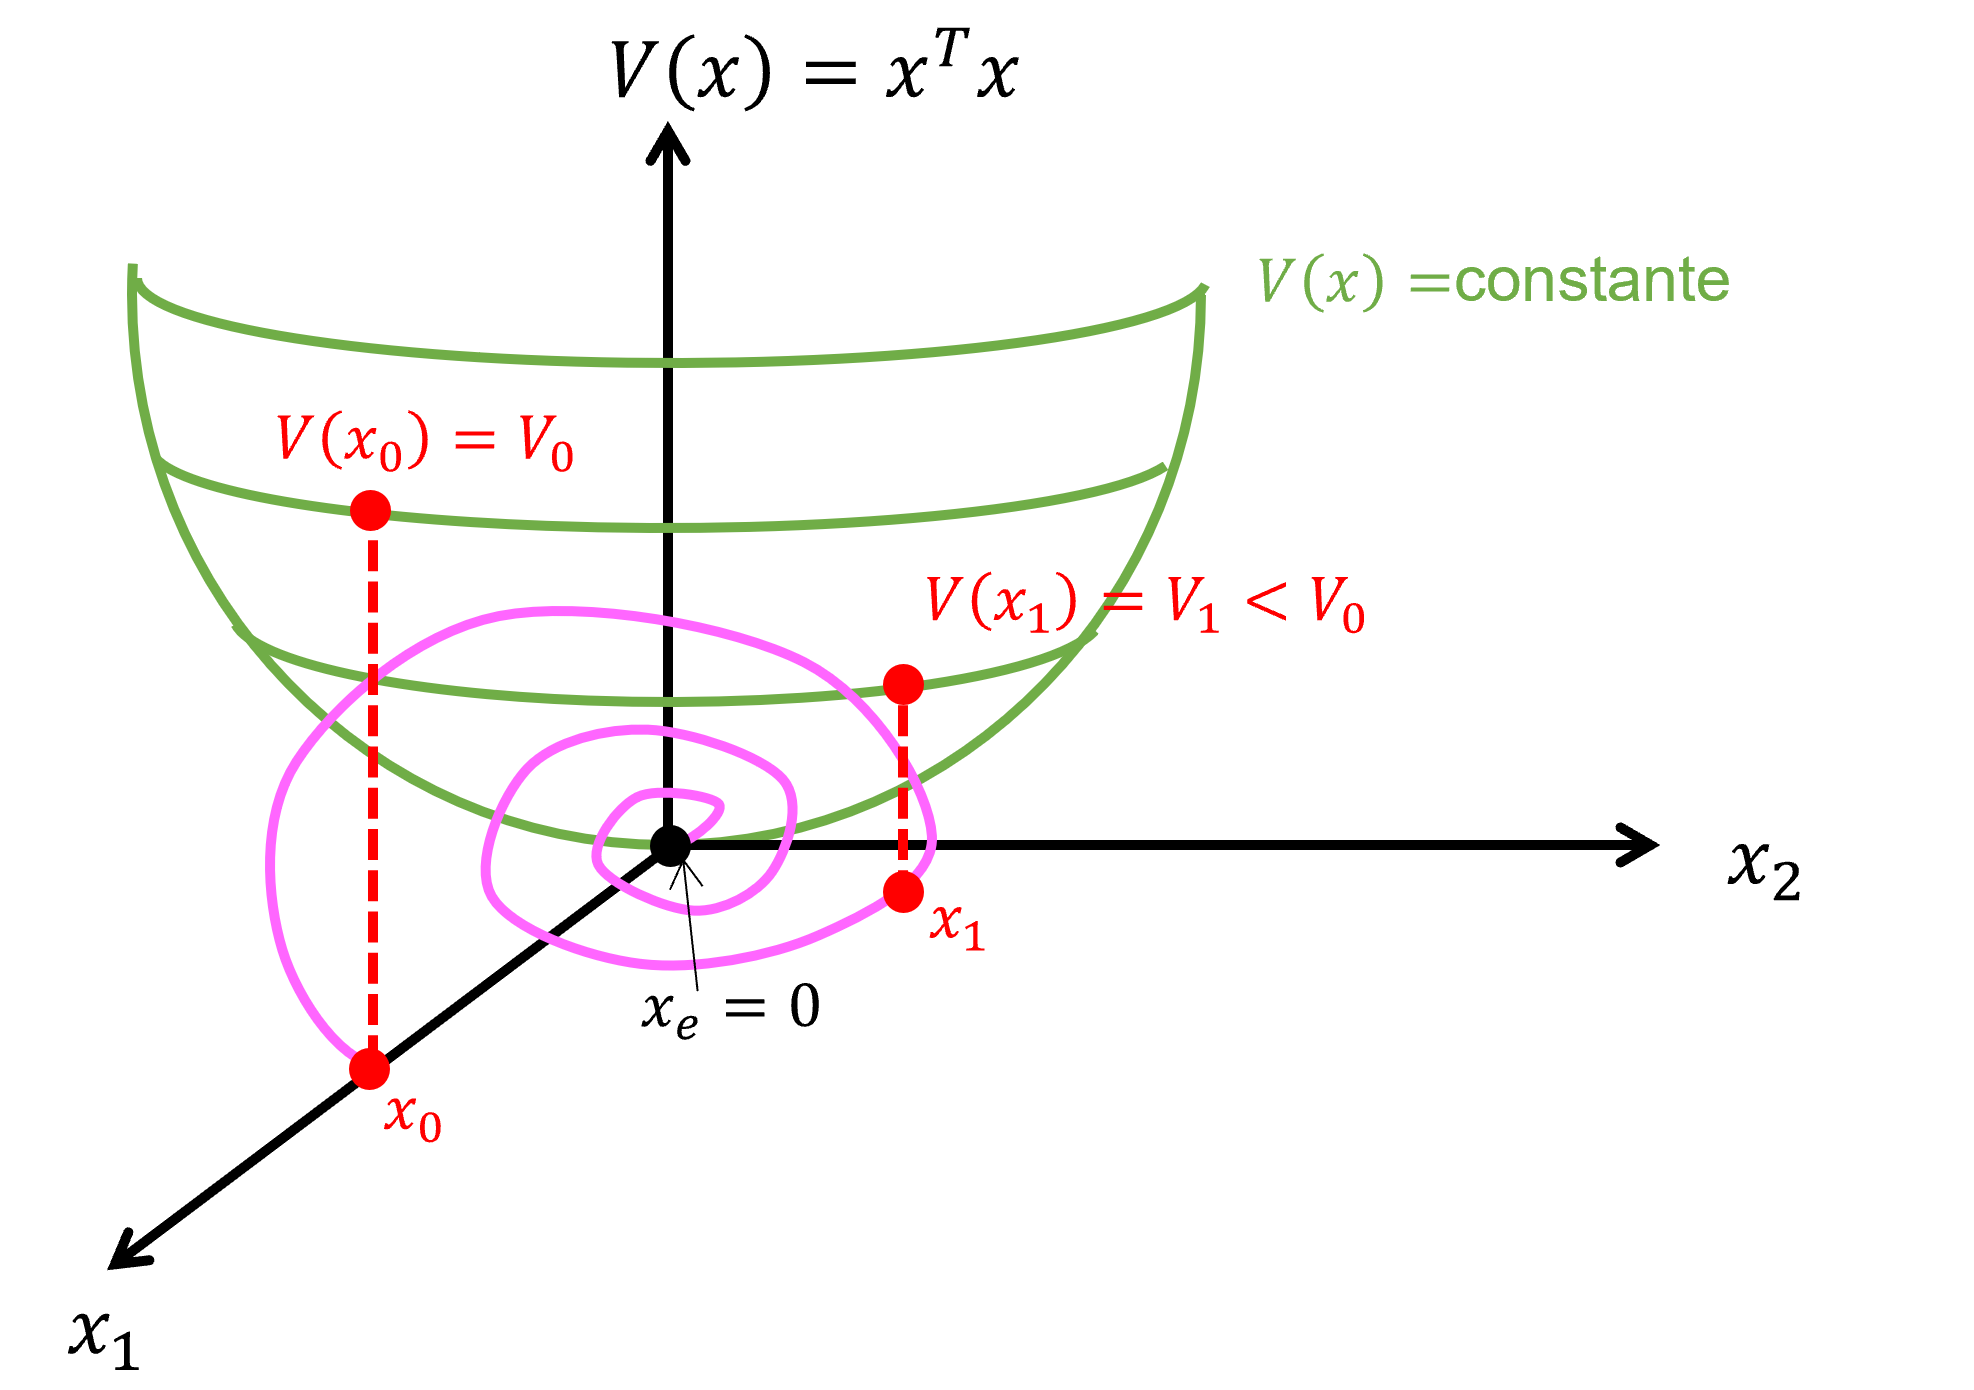
\includegraphics[scale=0.7]{Figuras/ilu_lyapunov.png}
\end{figure}

Notar que:
\begin{align*}
    \frac{dV(x)}{dt} < 0   
\end{align*}

Ocupando $V=V(x(t))$. Entonces:
\begin{align*}
    \frac{dV}{dt} &= \frac{\partial V}{\partial x}\cdot \frac{\partial x}{\partial t}  \quad \text{Regla de la cadena}\\
    &= \sum_{i=1}^n \frac{\partial V}{\partial x_i}\cdot\frac{\partial x_i}{\partial t}\\
    &= \begin{bmatrix}\frac{\partial V}{\partial x_1} &...& \frac{\partial V}{\partial x_n}\end{bmatrix}\begin{bmatrix}\dot{x}_1\\ \vdots \\ \dot{x}_n\end{bmatrix}\\
    &= \nabla V\cdot \dot{x}
\end{align*}

\begin{align*}
    \frac{dV}{dt}=\nabla V\cdot \dot{x}<0, ~\forall t
\end{align*}

Dibujemos una línea de contorno de $V(x)$: \\
\begin{figure}[H]
\centering
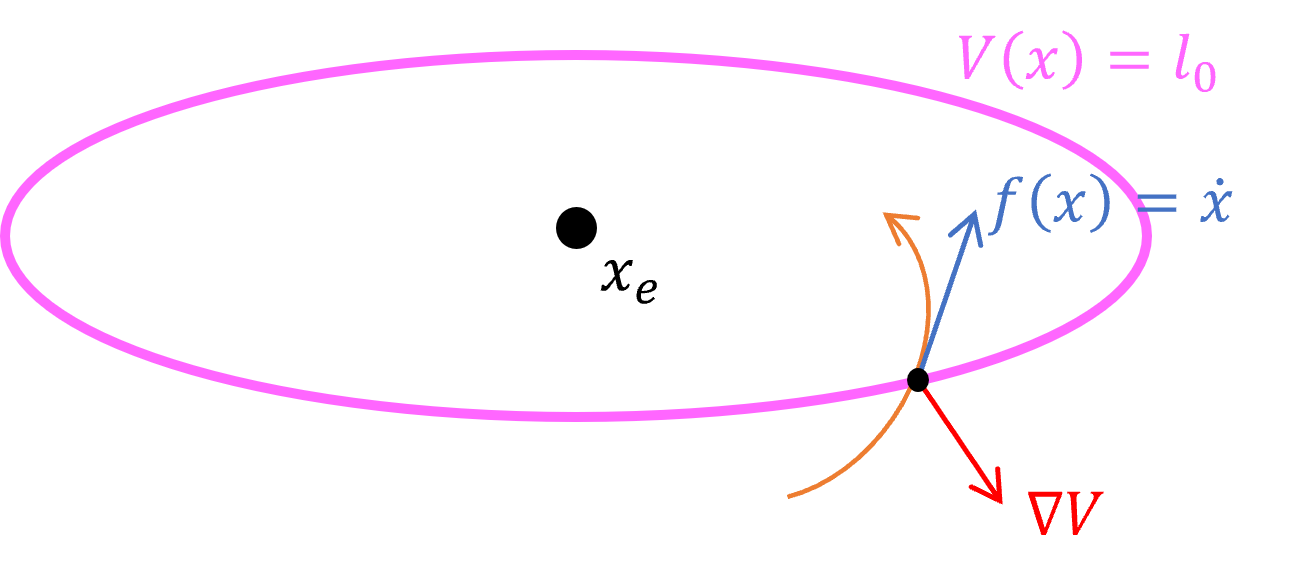
\includegraphics[scale=0.7]{Figuras/ilu_lyapunov2.png}
\end{figure}

\begin{align*}
    \nabla V\cdot f(x)<0 \Longrightarrow \text{Entonces el sistema se acerca a } x_e   
\end{align*}

$\Longrightarrow x_e$ es un punto de atracción o \emph{sumidero}.\\

\par Para el sistema LTI autónomo $\dot{x}=Ax$, y sea $V(x)=x^\top Px$, donde $P$ es una matriz definida positiva y simétrica.
$$\frac{dV}{dt}=\nabla V\cdot \dot{x}<0 $$ 

para un sistema asintóticamente estable.\\
\begin{align*}
    \nabla V=\frac{\partial}{\partial \tend{x}} (\tend{x}^\top \tenq{P}\tend{x}) = 2\tenq{P}\tend{x} \quad \text{Por demostrar}
\end{align*}

Entonces:
\begin{align*}
    \frac{dV}{dt} &= (2Px)^\top (Ax)= (2x^\top P^\top)(Ax)\\
    &= (x^\top P^\top)(Ax)+x^\top P^\top Ax\\
    &= (Px)^\top(Ax)+x^\top PAx\\
    &= (Ax)^\top(Px)+x^\top PAx\\
    &= x^\top A^\top Px+x^\top PAx\\
    &= x^\top (A^\top P+PA)x<0
\end{align*}

Por lo tanto, $A^\top P+PA \prec 0$ debe ser una matriz definida negativa para que el sistema sea asintóticamente estable.\\
\par Sea $Q$ una matriz definida positiva y simétrica, tal que:
\begin{align*}
    &\phantom{\Longrightarrow} A^\top P+PA = -Q\\
    &\Longrightarrow A^\top P+PA+Q = \emptyset \quad \text{Ecuación de Lyapunov}
\end{align*}

\underline{Teorema}: Dados $Q \succ 0$ y simétrico, existe un $P\succ 0$ simétrico que satisface:
$$A^\top P+PA+Q=\emptyset $$

entonces, $\dot{x}=Ax$ es asintóticamente estable.

\section{Controlabilidad}
% La controlabilidad es una propiedad de cualquier sistema dinámico.\\

Sea un sistema LTI: $\dot{x}=Ax+Bu$, $x\in \mathbb{R}^n$, $u\in\mathbb{R}^p$. Buscamos $u(t)$ tal que los estados vayan de $x(t)$ a cero en un tiempo finito $t_1$. \\
Recordar que la solución de un sistema LTI no autónomo es:
\begin{align*}
    x(t)=\phi(t)x_0+\int_0^t \phi(t-\tau)Bu(\tau)d\tau    
\end{align*}
Luego, si $x(t_1) = 0$
\begin{align*}
    0=\phi(t_1)x_0+\int_0^{t_1} \phi(t_1-\tau)Bu(\tau)d\tau
\end{align*}

Considerando la propiedad: $\phi(t_1-\tau)=e^{A(t_1-\tau)}=e^{At_1}\cdot e^{-A\tau}=\phi(t_1)\phi(-\tau)$. Entonces:

\begin{align*}
    0 &=\phi(t_1)\left[x_0+\int_0^{t_1}\phi(-\tau)Bu(\tau)d\tau\right] \\
    \Longrightarrow -x_0 &= \int_0^{t_1}\phi(-\tau)Bu(\tau)d\tau
\end{align*}

Por el teorema de Cayley-Hamilton:
\begin{align*}
    \phi(-\tau)=m_0(\tau)I+m_1(\tau)A+m_2(\tau)A^2+...+m_{n-1}(\tau)A^{n-1}
\end{align*}

Entonces:
\begin{align*}
    -x_0 &= \int_0^{t_1}\left[m_0(\tau)B+m_1(\tau)AB+m_2(\tau)A^2B+...+m_{n-1}(\tau)A^{n-1}B \right]u(\tau)d\tau\\
    \Longrightarrow -x_0 &= \int_0^{t_1} \sum_{j=0}^{n-1}A^jBm_j(\tau)u(\tau)d(\tau)\\
    \Longrightarrow -x_0 &= \sum_{j=0}^{n-1}A^jB \int_0^{t_1} m_j(\tau)u(\tau)d\tau
\end{align*}

Cada término de la integral es un vector constante de dimensión $p\times 1$
\begin{align*}
    \Longrightarrow v_j := \int_0^{t_1}m_j(\tau)u(\tau)d\tau
\end{align*}

\begin{align*}
    \Longrightarrow -x_0 &= \sum_{j=0}^{n-1}A^jBv_j =Bv_0+ABv_1+...+A^{n-1}Bv_{n-1}\\
     \Longrightarrow -x_0 &= \left[
    \begin{array}{c|c|c|c|c}
     B & AB & A^2B & ... & A^{n-1}B
    \end{array}\right] \left[
    \begin{array}{c}
     v_0\\ \hline v_1 \\ \hline v_2 \\ \hline \vdots \\ \hline v_{n-1} 
    \end{array}\right]
\end{align*}

Por lo tanto, se define la \emph{Matriz de Controlabilidad} $\mathcal{C}$:
\begin{align*}
    \mathcal{C}=\left[
    \begin{array}{c|c|c|c|c}
     B & AB & A^2B & ... & A^{n-1}B
    \end{array}\right]
\end{align*}

Este resultado indica que cualquier vector $-x_0$ puede ser expresado como una combinación lineal de las columnas de la matriz $\mathcal{C}$. Esta matriz $\mathcal{C}$ debe tener rango igual a $n$ para escribir $-x_0 \in \mathbb{R}^n$.\\

\underline{Por lo tanto, un sistema LTI es controlable ssi $\text{rank}(\mathcal{C})=n$}. \\

\underline{Nota}: Si $\text{rank}(\mathcal{C})= n_e < n$, entonces el sistema tiene no más de $n_e$ estados controlables.\\
\par \underline{Definición}: Si el sistema tiene estados inestables, pero controlables, entonces se dice que estos estados son \textbf{estabilizables}. Por lo tanto, puede diseñar $u(t)$ tal que el sistema cerrado tenga todos sus estados estables.\\

\underline{Nota}: Sea el sistema LTI, $\dot{x}=Ax+Bu$, y sea $T$ una matriz de transformación tal que $x=Tz$, donde $\dot{z}=A_cz+B_cu$, es una realización CCF. Entonces, el sistema es controlable ssi $T$ existe.

\section{Observabilidad}
Asuma el sistema LTI autónomo:
\begin{align*}
    \dot{x} &= Ax, \quad x\in\mathbb{R}^n\\
    y &= Cx, \quad y\in\mathbb{R}^r
\end{align*}

\begin{align*}
    \begin{array} {|c|}
  \hline \text{Caja}\\ 
  \text{Negra} \\
  \hline 
\end{array} \longrightarrow y\in\mathbb{R}^r
\end{align*}

Sabemos que la solución $x(t)$: 

\begin{align*}
    x(t) = \phi (t) x_0 \Longrightarrow y(t) = C x(t) = C \phi (t) x_0    
\end{align*}

Además, utilizando el Teorema de Cayley-Hamilton:
\begin{align*}
    y(t) &= Ce^{At}x_0\\
    y(t) &= C\left[l_0(t)I+l_1(t)A+l_2(t)A^2+...+l_{n-1}(t)A^{n-1} \right]x_0\\
    y(t) &= \left[
    \begin{array}{c|c|c|c|c}
     l_0(t) & l_1(t) & l_2(t) & ... & l_{n-1}(t)
    \end{array}\right] \left[
    \begin{array}{c}
     C\\ \hline CA \\ \hline CA^2 \\ \hline \vdots \\ \hline CA^{n-1} 
    \end{array}\right] x_0
\end{align*}

Se define:
\begin{align*}
    \mathcal{O}=\left[
    \begin{array}{c}
     C\\ \hline CA \\ \hline CA^2 \\ \hline \vdots \\ \hline CA^{n-1} 
    \end{array}\right] \quad \text{Matriz de observabilidad}
\end{align*}

Si $\mathcal{O}$ no es de rango completo, entonces podemos elegir $x_0\neq 0$ tal que $y(0)=0$, porque $t_0$ puede producir el mismo resultado. \\
\par \underline{Por lo tanto, un sistema LTI es observable ssi $\text{rank}(\mathcal{O})=n$}\\
\par \underline{Definición}: Si un estado es inestable, pero observable, entonces dicho estado se dice que es \textbf{detectable}. 


\chapter{Vibraciones Estocásticas}

\section{Proceso Estocástico}
Una \textcolor{red}{variable aleatoria} $X$ toma una ``realización'' (valor), no hay un efecto del tiempo. \\

Ejemplos de variables aleatorias:
\begin{itemize}
    \item Período de retorno (``ocurrencia'') de un terremoto % $ > M_w8.5$
    \item Módulo de Young de un material (Hormigón: $E_c$)
    \item Resistencia característica (Acero: $F_y$)
    \item Geometría
    \item Intensidad de un terremoto en un sitio específico.
\end{itemize}

Un \textcolor{red}{proceso estocástico} (p.e.) es una colección de variables aleatorias para cada $t \in T$. Para los casos prácticos de este curso, la indexación $t$ puede ser el tiempo, por lo que la colección es secuencial. Además, un p.e. puede ser continuo (imposible de hacer en computador) o discreto (conjunto/arreglo/vector). \\
\begin{align*} 
    \Longrightarrow \{X(t): t \in T\} =\{X(t_1), X(t_2), ..., X(t_m)\}
\end{align*}

Una realización de un proceso estocástico corresponde a la realización de todas las variables aleatorias de su colección. \\

Realización 1: 
\begin{figure}[H]
\centering
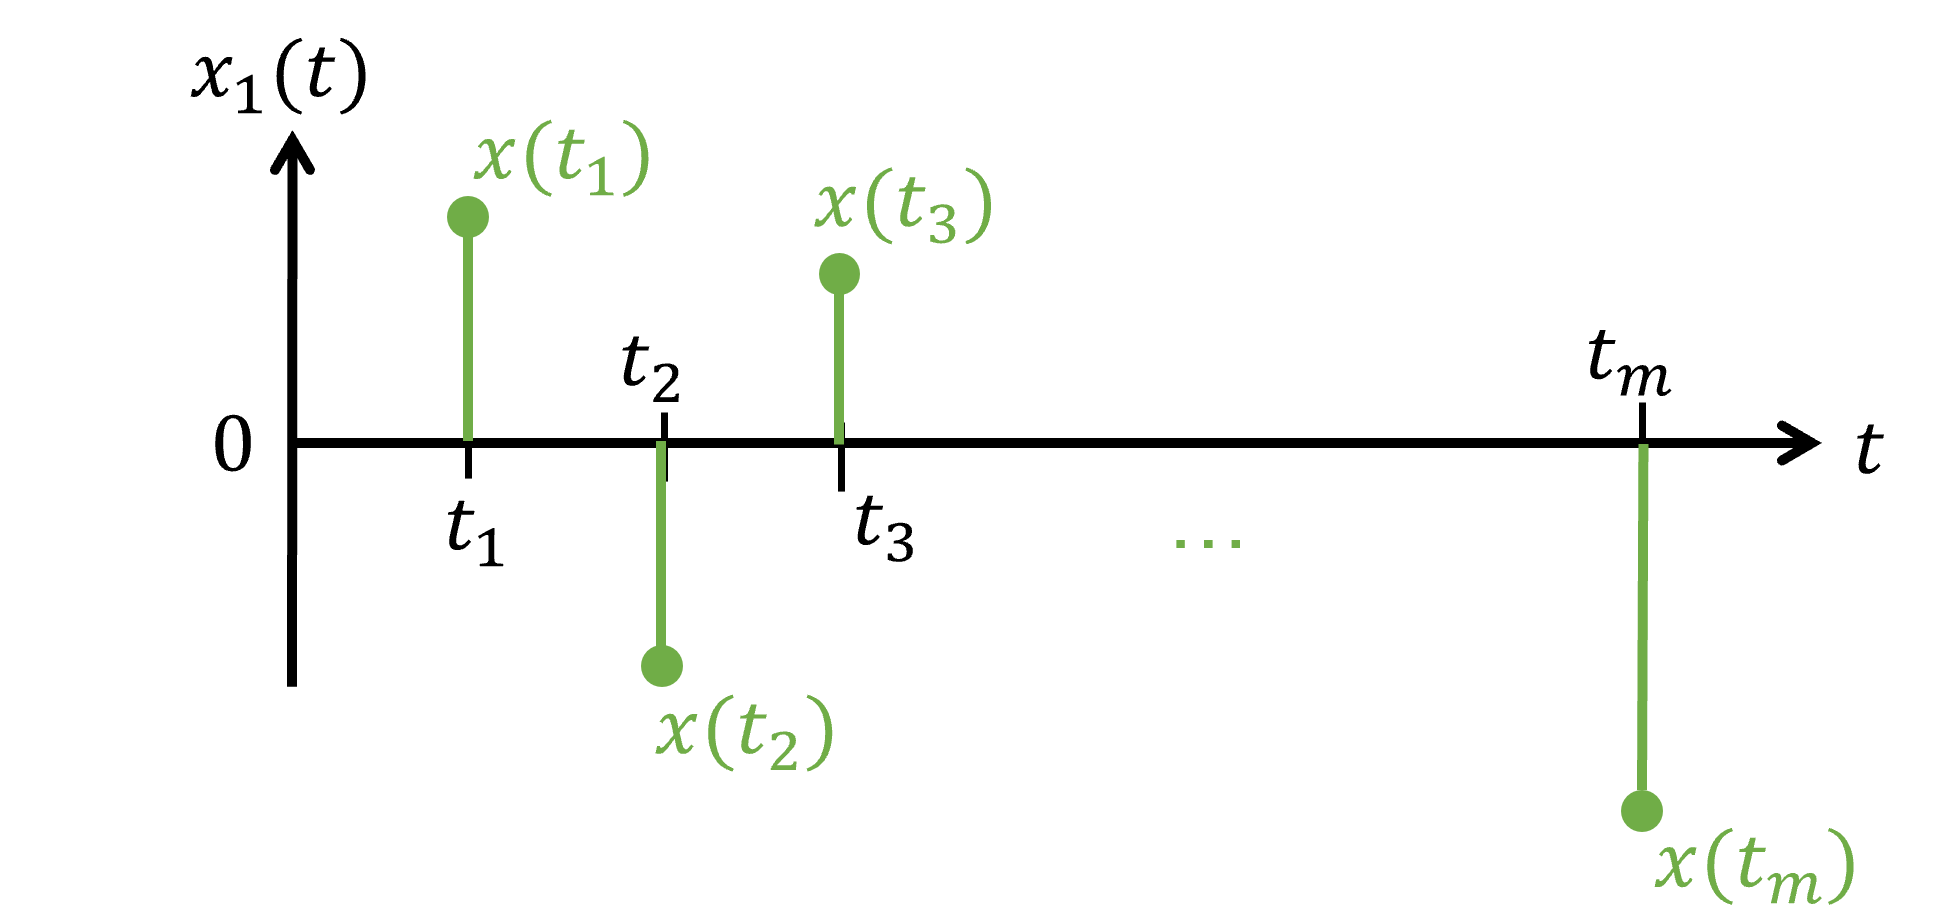
\includegraphics[scale=0.7]{Figuras/pe.png}
\end{figure}

Realización 2: 
\begin{figure}[H]
\centering
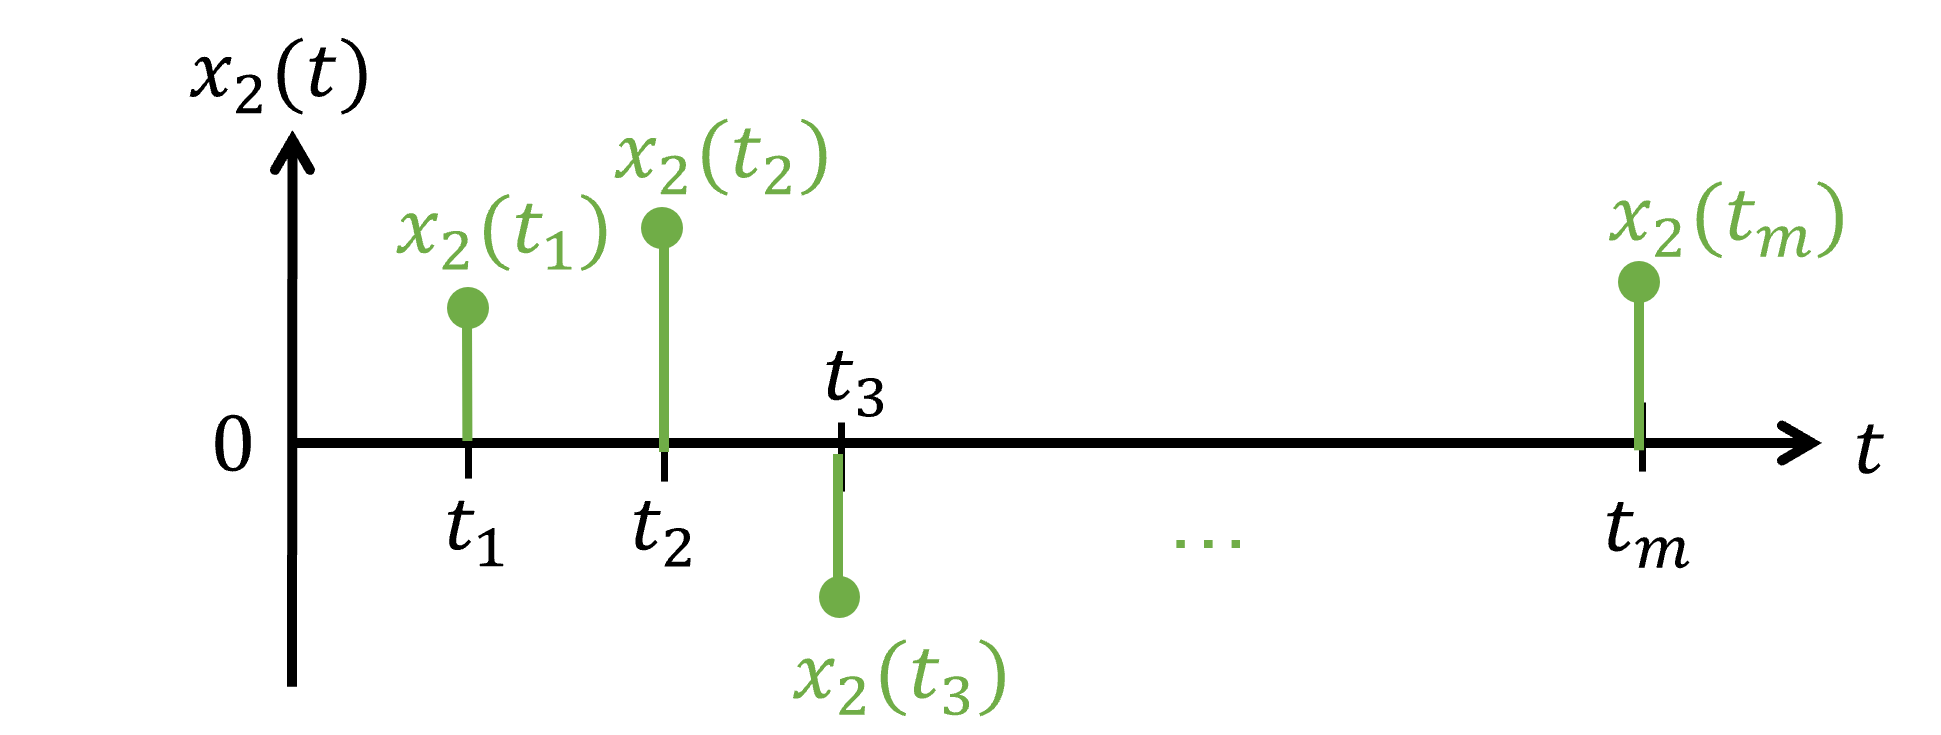
\includegraphics[scale=0.7]{Figuras/pe2.png}
\end{figure}

\par Ejemplos de p.e. para aplicación en ingeniería estructural y sísmica:
\begin{itemize}
    \item Vibraciones aleatorias
    \item Registro de aceleración de un terremoto
    \item Presión del viento
    \item Carga de tráfico un puente
\end{itemize}

\par Existen 2 formas de describir un p.e. $\{X(t)$, $t\in T\}$:
\begin{enumerate}
    \item Función de distribución conjunta (ej: CDF)
    \begin{align*}
        \mathbb{P}[X(t_1)\leq x_1 \cap X(t_2)\leq x_2 \cap ... \cap X(t_m) \leq x_m ] = F_X(x_1,x_2,...,x_m;t_1,t_2,...,t_m)
    \end{align*}
    \item Momentos estocásticos $\Longrightarrow$ momentos de 1er y 2do orden
    \begin{itemize}
        \item Media $(m \times 1)$: $$\mu _X(t_i)=\mathbb{E}\{X(t_i)\}$$
        \item Varianza $(m \times 1)$: $$\sigma _X^2(t_i)=\mathbb{E}\{[X(t_i)-\mu_X(t_i)]^2\}$$
        \item Función de auto-correlación $(m \times m)$: $$R_{XX}(t_i,t_j)=\mathbb{E}\{X(t_i)X(t_j)\}$$
        \item Función de auto-covarianza $(m \times m)$: $$\Gamma_{XX}(t_i,t_j)=\mathbb{E}\{[X(t_i)-\mu_X(t_i)][X(t_j)-\mu_X(t_j)]\}$$ $$\Gamma_{XX}(t_i,t_j)=R_{XX}(t_i,t_j)-\mu_X(t_i)\mu_X(t_j)$$
        \item Coeficiente de correlación $(m \times m)$: $$\rho_{XX}(t_i,t_j) = \frac{\Gamma_{XX}(t_i,t_j)}{\sigma_X(t_i)\sigma_X(t_j)}$$ \\

        Notar que: $$\rho_{XX}(t_i, t_i) = 1$$\\
        
        Interpretación: ``medida de independencia lineal entre variables aleatorias''. \\
        \begin{figure}[H]
            \centering
            \subfigure[]{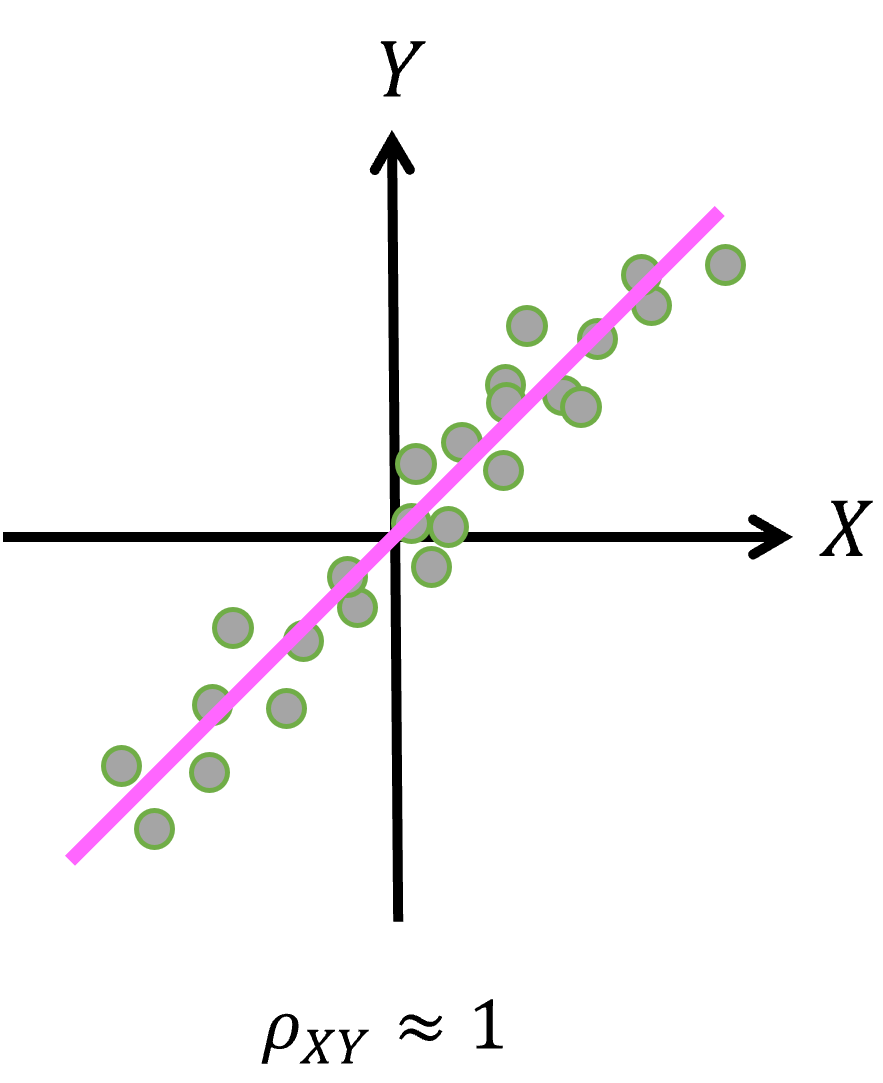
\includegraphics[scale=0.7]{Figuras/rho1.png}}
            \subfigure[]{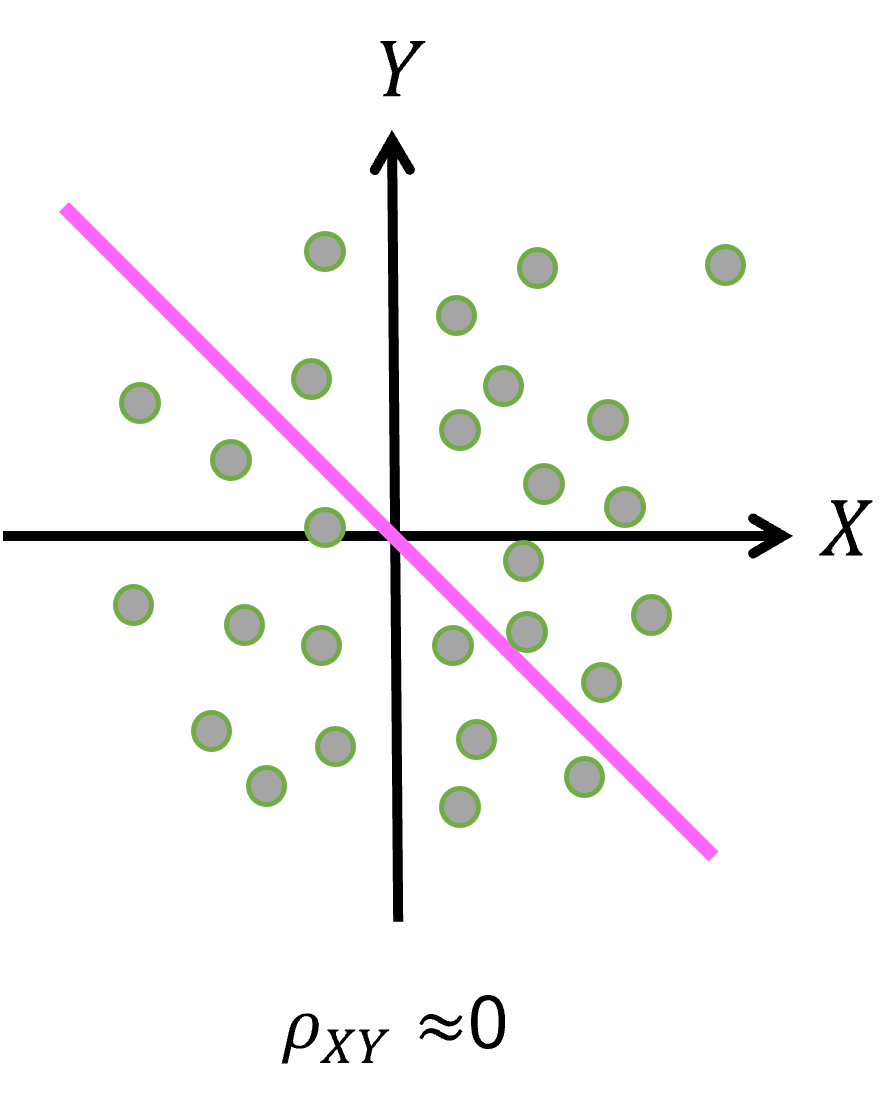
\includegraphics[scale=0.7]{Figuras/rho0.png}}
        \end{figure}
        Notas: \begin{itemize}
            \item $|\rho_{XX}(t_i,t_j)| \leq 1$
            \item Si $\rho_{XX}(t_i,t_j)=0$, $\forall t_i \neq t_j$, entonces el p.e. es un proceso descorrelacionado (por ejemplo: ruido blanco).
        \end{itemize}
    \end{itemize}
\end{enumerate}

En caso de dos procesos estocásticos, $\{X(t)$, $t \in T_X\}$ y $\{Y(t)$, $t \in T_Y\}$ dos procesos estocásticos (ej.: sismo y respuesta estructural):
\begin{itemize}
    \item Función de correlación cruzada: $$R_{XY}(t_i,t_j)=\mathbb{E}\{X(t_i)Y(t_j)\} $$
    \item Función de covarianza cruzada:
    $$\Gamma_{XY}(t_i,t_j) =\mathbb{E}\{ [X(t_i)-\mu_x(t_i)][Y(t_j)-\mu_y(t_j)]\} $$
    $$\Gamma_{XY}(t_i,t_j) = R_{XY}(t_i, t_j)-\mu_X(t_i)\mu_Y(t_j) $$ 
    \item Coeficiente de correlación cruzado: $$\rho_{XY}(t_i,t_j)=\frac{\Gamma_{XY}(t_i,t_j)}{\sigma_X(t_i)\sigma_Y(t_j)} $$
\end{itemize}

% Ej.: p.e. de terremoto (X) y p.e. de respuesta estructural (Y), estos están correlacionados. githu

\section{Clasificación de P.E.}
\begin{enumerate}
    \item \underline{P.E. no estacionario}: La distribución de probabilidad del p.e. depende del tiempo. Las variables aleatorias de la colección no tienen la misma distribución.
    \begin{figure}[H]
    \centering
    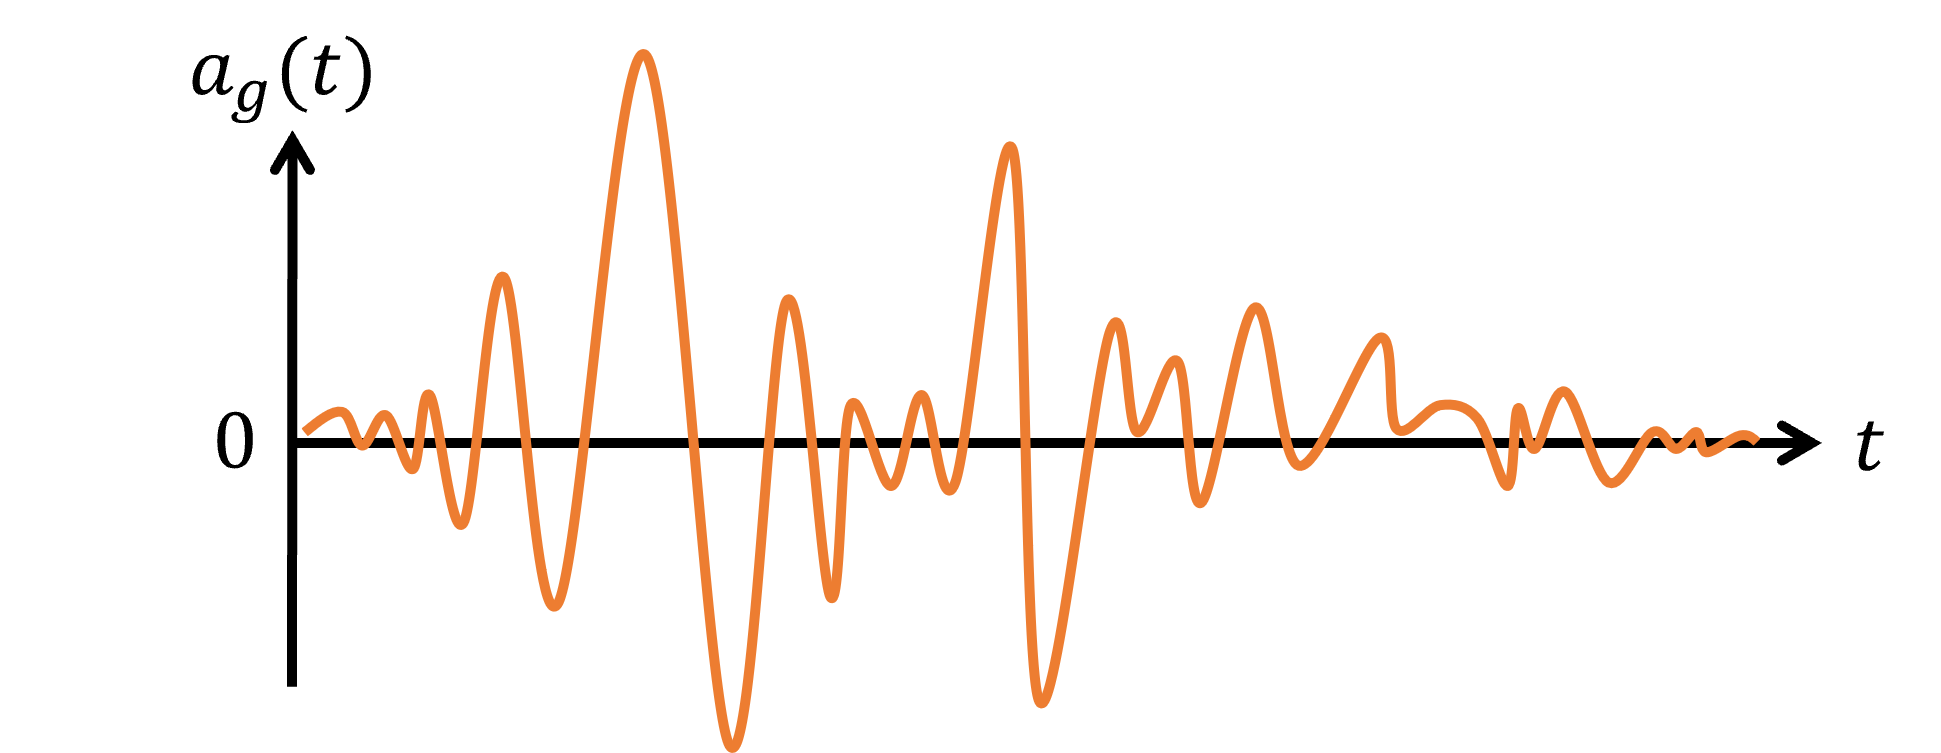
\includegraphics[scale=0.7]{Figuras/penoesatacionario.png}
    \end{figure}
    
    \item \underline{P.E. Estrictamente estacionario}: La distribución de probabilidad del p.e. no cambia con un retraso en el tiempo:
    \begin{equation*}
        F_X(x_1,...,x_m; t_1,...,t_m) = F_X(x_1,...,x_m; \textcolor{brown}{t_1 + \tau,...,t_m + \tau})
    \end{equation*}
    \begin{figure}[H]
    \centering
    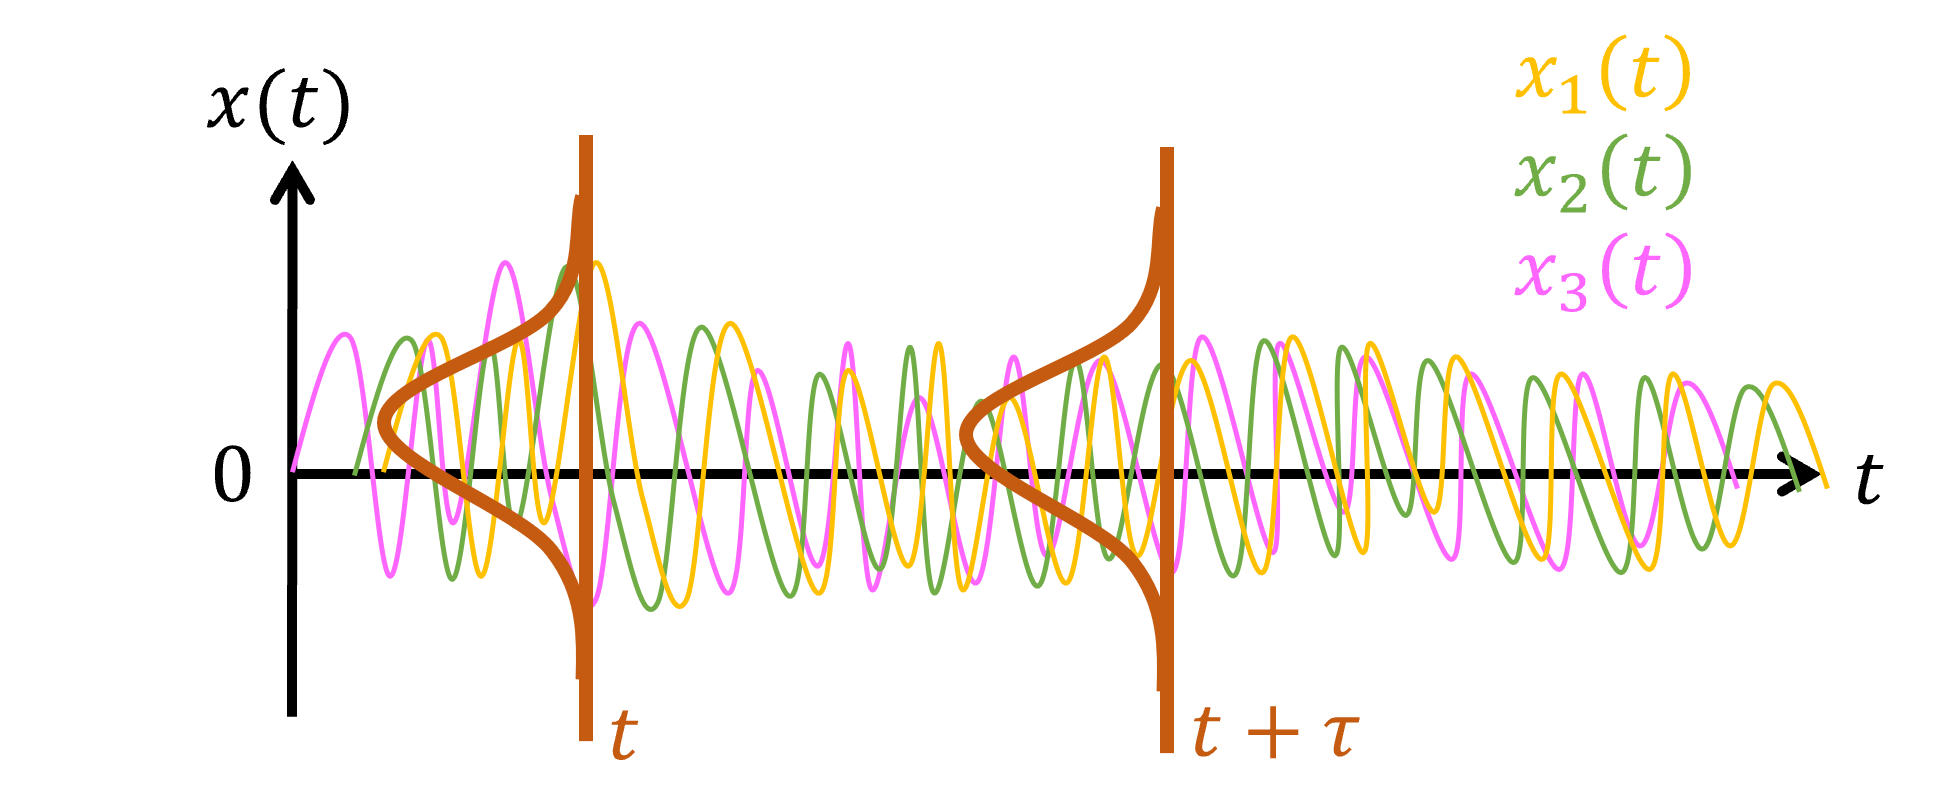
\includegraphics[scale=0.7]{Figuras/peestricto.png}
    \end{figure}
    \item \underline{P.E. Débilmente estacionario}: Estadísticos de 2do orden son finitos y no varían en el tiempo
    \begin{align*}
        &\phantom{\Longrightarrow}\mu_X(t_i)=\mu_X(t_j) = cste, \quad \sigma_X^2(t_i)=\sigma_X^2(t_j)=cste\\
        &\Longrightarrow R_{XX}(t_1,t_2) = R_{XX}(t_2-t_1)
    \end{align*}
\end{enumerate}

\section{P.E. Gaussiano}
Un p.e. $\{X(t)$, $t \in T\}$, se llama un p.e. Gaussiano si, para cada conjunto $\{t_1,t_2,...,t_m\}\in T$, las ``m'' variables aleatorias $X(t_1)$, $X(t_2)$, $...,$ $X(t_m)$ son distribuidas normales multivariadas.
\begin{align*}
    \{X(t), t \in T\}\sim~ N\big(\mu_X,\Gamma_{XX}\big)
\end{align*}
donde $\mu_X$ es el vector de las medias de las variables aleatorias del p.e. y $\Gamma_{XX}$ es la matriz de auto-covarianza. \\

\underline{Notas}:
\begin{itemize}
    \item Un p.e. Gaussiano y débilmente estacionario es estrictamente estacionario.
    \item Un p.e. Gaussiano preserva las transformaciones lineales, y esto es extremadamente útil en los problemas de sistemas lineales que se verán más adelante.
\end{itemize}

\section{Función de Autocorrelación}
Dado $\{X(t), t \in T\}$ un w.s.s., la \emph{función de autocorrelación} $R_{XX}(\tau) = R_X(\tau)$ se define como:
\begin{align*}
    R_{X}(\tau)=\mathbb{E}\{X(t)X(t+\tau)\}
\end{align*}

\underline{Características de $R_X(\tau)$}:
\begin{enumerate}
    \item $R_X(\tau)$ es una función par
    \begin{align*}
        R_X(\tau)=R_X(-\tau)
    \end{align*}
    \item $R_X(\tau)$ debe ser finita. Adicionalmente.:
    \begin{align*}
        |R_X(\tau)|&\leq R_X(0)\\
        \Longrightarrow R_X(0)&=\mathbb{E}\{X^2(t)\}=\sigma^2_X(t)+\mu_X^2(t)
    \end{align*}
    En $\tau=0$, $R_X(0)$ entrega el máximo valor de la media cuadrada del p.e. $\{X(t), t \in T\}$.
    \item $R_X(\tau)$ es una función definida positiva.\\
    $\Longrightarrow$ Para cualquier función $g(t)$, si:
    \begin{align*}
        g(t_1)R_X(t_1-t_2)g(t_2)\geq 0
    \end{align*}
    Por lo tanto, $R_X(\tau)$ es definida positiva siempre.
    \item $R_X(\tau)$ es continua en $\tau$.
\end{enumerate}

\section{Densidad de Poder Espectral (power spectral density, PSD)}
\underline{Definición}: Densidad de poder espectral (PSD) (Teorema de Wiener-Khintchine).\\
\par Sea $X=\{X(t): t\in T\}$ un p.e. w.s.s. (weakly strictly stationary), con función de autocorrelación $R_x(\tau)$. La función de densidad de poder espectral se define como la \emph{transformada de fourier} de la \emph{función de autocorrelación}:
\begin{align*}
    S_X(\omega) &=\mathcal{F}\{R_X(\tau)\}\\
    R_X(\tau) &=\mathcal{F}^{-1}\{S_X(\omega)\}
\end{align*}

\par \underline{Propiedades PSD}:
\begin{enumerate}
    \item Función real
    \item Función simétrica
    \item Definida positiva
    \item Área bajo la curva de $S_X(\omega)$ es igual a $\mathbb{E}\{X^2(t)\} = \sigma^2_X(t) + \mu^2_X(t) = R_X(\tau=0)$
\end{enumerate}
\begin{figure}[H]
\centering
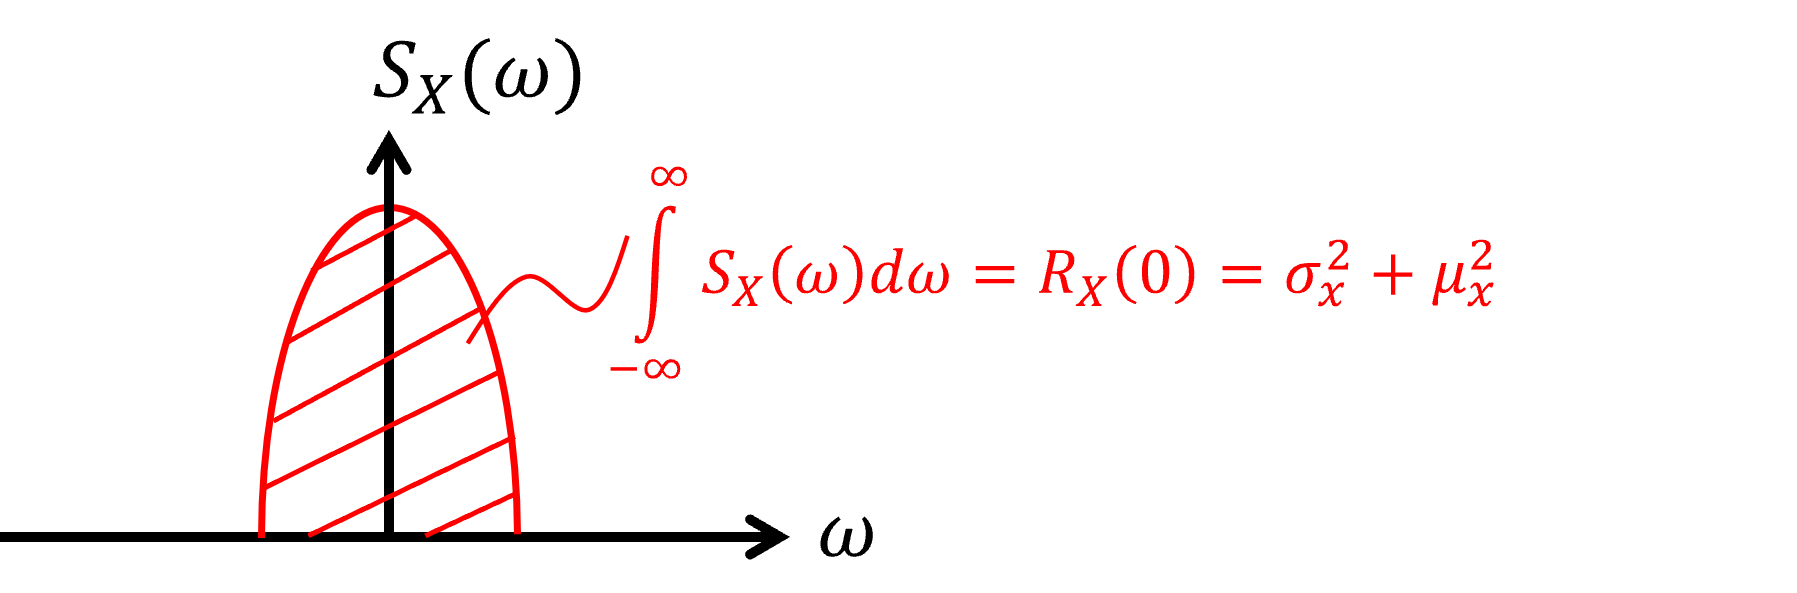
\includegraphics[scale=0.7]{Figuras/PSD.png}
\end{figure}

\section{Ruido blanco}
Sea $X=\{X(t): t\in T\}$ un p.e. w.s.s. Gaussiano, con $\mu_X=0$, $X$ es un ruido blanco si su PSD es constante:
\begin{align*}
    S_X(\omega) &= S_0, \quad \forall \omega \in (-\infty,+\infty)\\
    \Longrightarrow R_X(\tau) &= 2\pi S_0\delta (\tau)
\end{align*}

donde $\delta(\tau)$ es el delta de Dirac.
\begin{figure}[H]
\centering
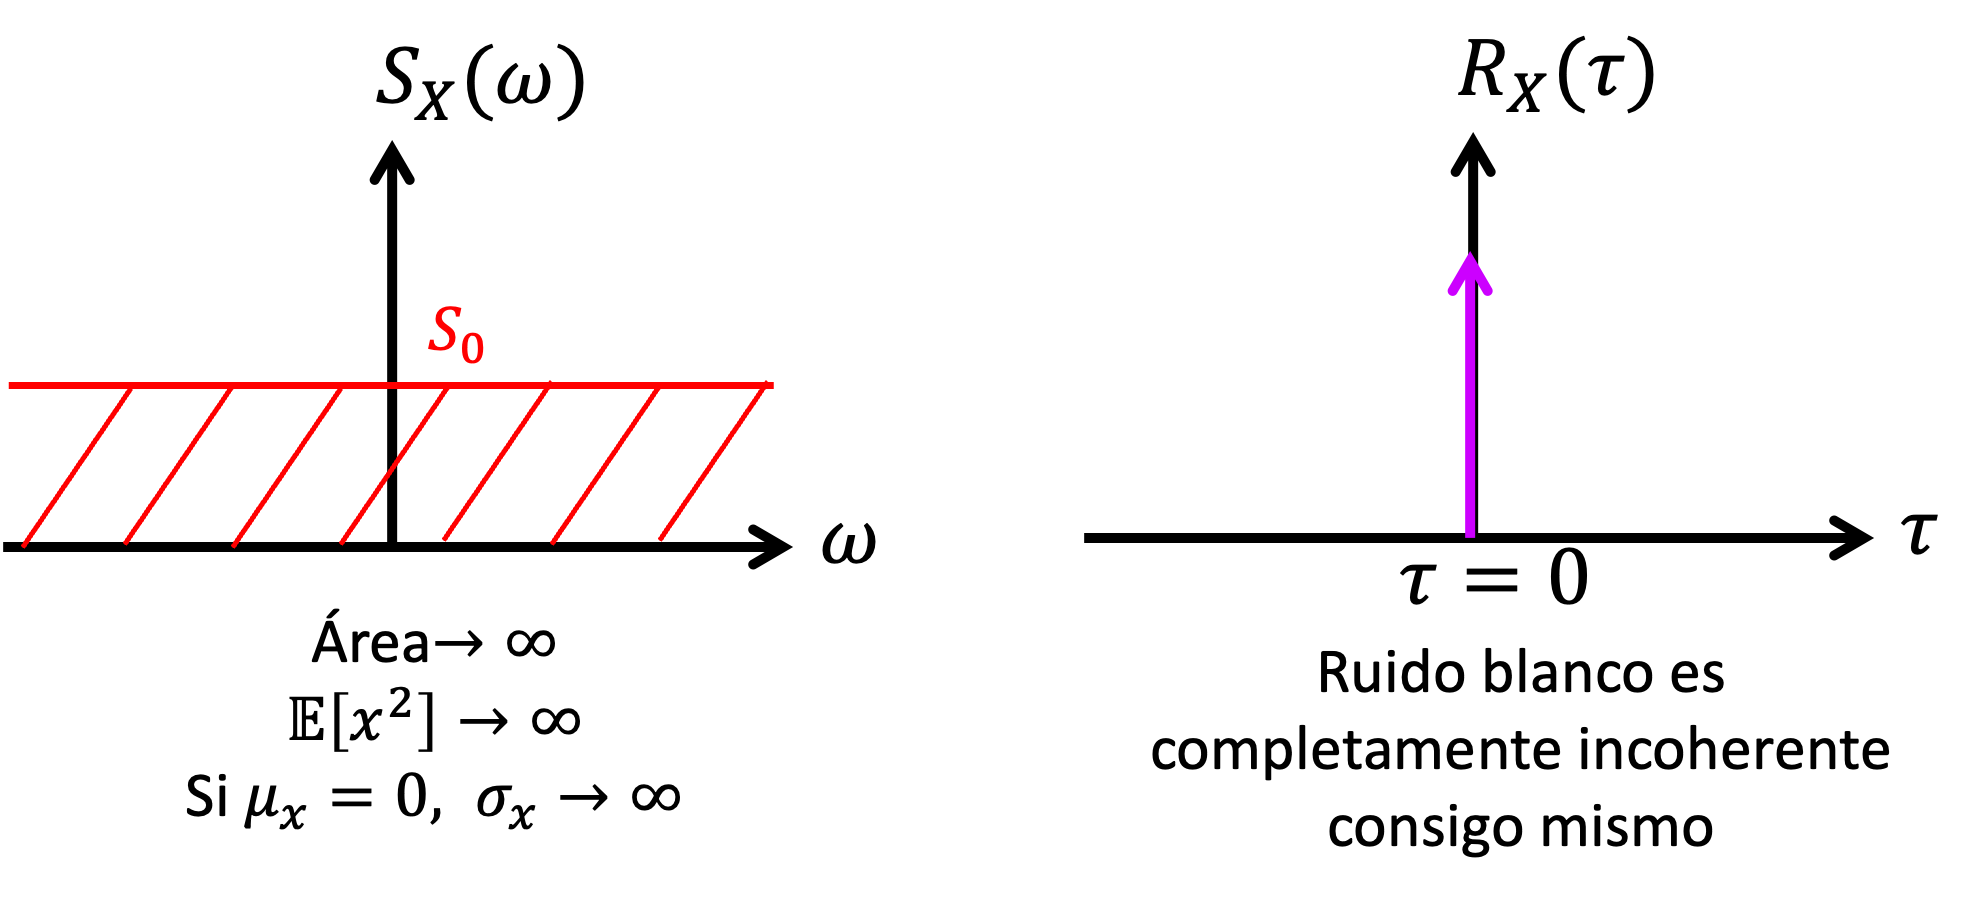
\includegraphics[scale=0.7]{Figuras/ruidoblanco.png}
\end{figure}


\subsection{Ruido blanco de banda limitada (band-limited white noise, BLWN)}
Sea $X$ un p.e., w.s.s., es un \emph{ruido blanco de banda limitada} (BLWN) si:
\begin{align*}
    S_X(\omega) & = \left\{
\begin{array}{ll}
      S_0 & |\omega|\leq \omega_c \\
      0 & |\omega|> \omega_c \\
\end{array} 
\right. \\
    R_X(\tau) & = R(0)\frac{\sin(\omega_c \tau)}{\omega_c \tau}\\
    & = R(0)\text{sinc}(\omega_c \tau)
\end{align*}

\begin{figure}[H]
\centering
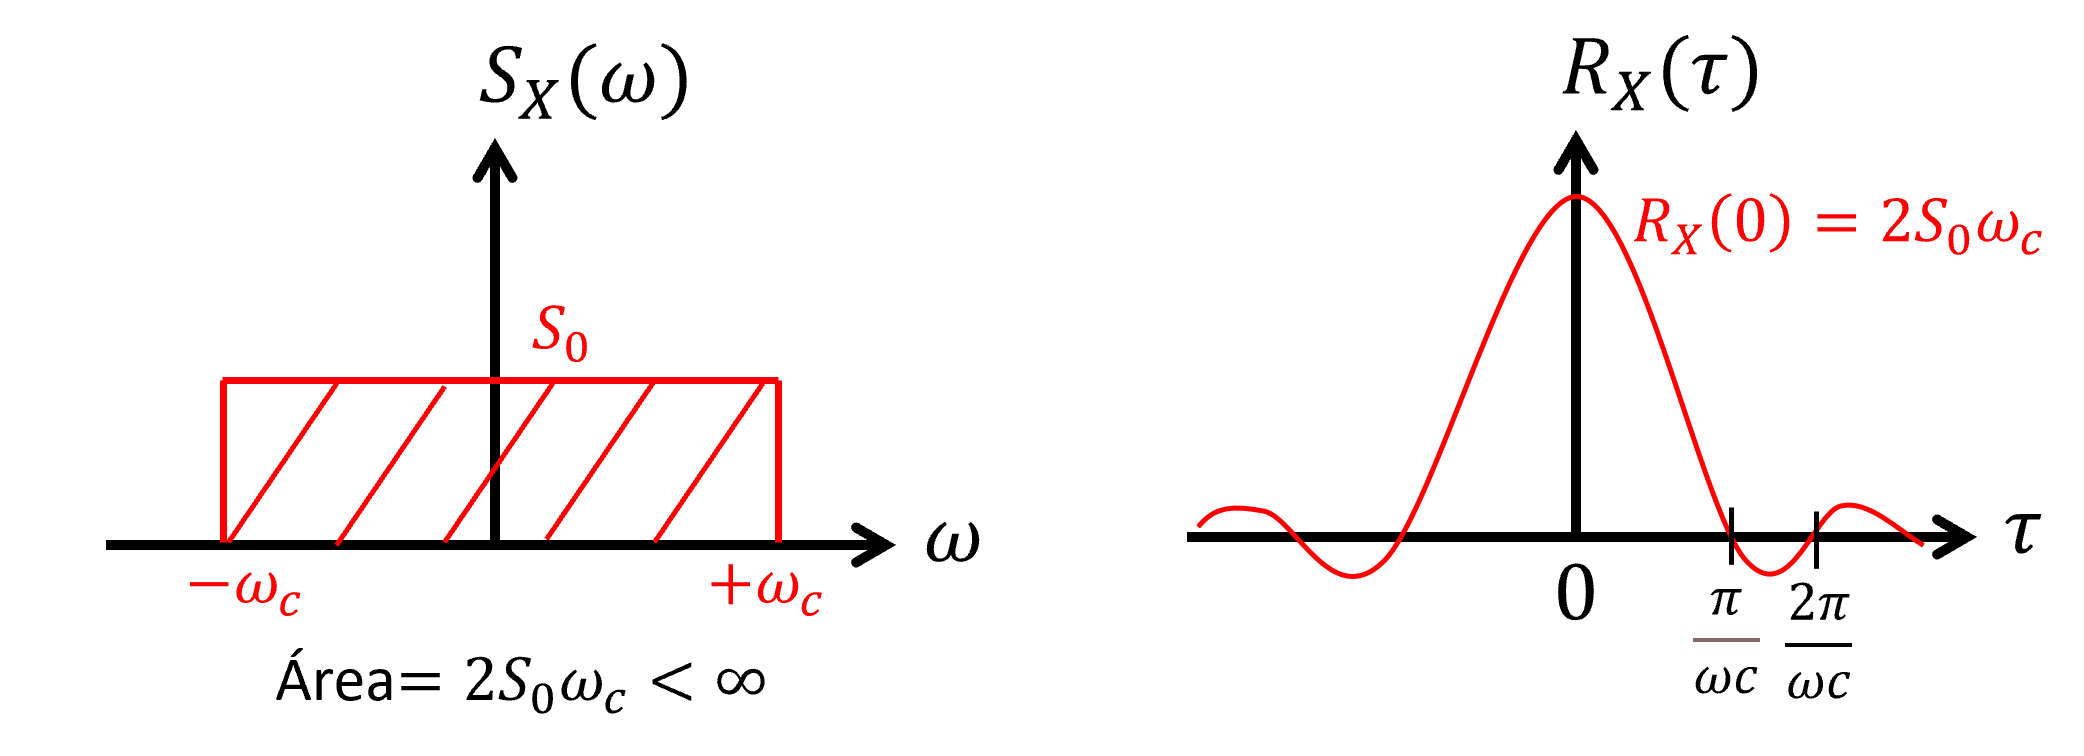
\includegraphics[scale=0.7]{Figuras/BLWN.png}
\end{figure}

Nota: a veces este p.e. se conoce como un filtro de paso bajo (``low-pass filter'').

\section{Ergocidad}
Sea $X=\{X(t): t\in T\}$ un p.e. estacionario, se dice que $X$ es ergódico si:
\begin{itemize}
    \item Ergódico en la media: 
    \begin{align*}
        \overline{\mu_X(t)}=\mu_X(t)
    \end{align*}
    \begin{itemize}
        \item $\overline{\mu_X(t)}$: media tiempo
        \item $\mu_X(t)$: media conjunto
    \end{itemize}
    \item Ergódico en el valor cuadrado:
    \begin{align*}
        \overline{\mathbb{E}\{X^2(t)\}} =\mathbb{E}\{X^2(t)\} 
    \end{align*}
    \begin{itemize}
        \item $\overline{\mathbb{E}\{X^2(t)\}}$: valor cuadrado tiempo
        \item $\mathbb{E}\{X^2(t)\}$: valor cuadrado conjunto
    \end{itemize}
    \item Ergódico en la correlación:
    \begin{align*}
        \overline{R_X(\tau)} = R_X(\tau)
    \end{align*}
    \begin{itemize}
        \item $\overline{R_X(\tau)}$: autocorrelación tiempo
        \item $R_X(\tau)$: autocorrelación conjunto
    \end{itemize}
\end{itemize}

\underline{Nota}: Un Ruido blanco es un p.e. Gaussiano, Ergódico.

\section{Respuesta estocástica de sistemas lineales}
Sea un sistema LTI:
\begin{align*}
    \tend{\dot{x}} =\tenq{A}\tend{x} + \tenq{B}u(t), \quad \tend{x}(0)=\tend{0}
\end{align*}
y asuma que $u(t)$ es un p.e. w.s.s., $\mu_U(t) = 0$. \\

\par \underline{Objetivo}: Determinar la respuesta $x(t)$, p.e. w.s.s., $\mu_X=0$\\
\par Calculemos la autocovarianza de $\tend{x}(t)$
\begin{align*}
    \tenq{\Gamma}_X(t)=\mathbb{E}[XX^\top]=
\end{align*}

La derivada de $\tenq{\Gamma}_X(t)$:
\begin{align*}
    \frac{d}{dt}\tenq{\Gamma}_X(t)&=\frac{d}{dt}\mathbb{E}[XX^\top]=\mathbb{E}\bigl[\frac{d}{dt}(XX^\top)\bigr]\\
    &= \mathbb{E}[\dot{X}X^\top+X\dot{X}^\top]\\
    &= \mathbb{E}\Bigl[(AX+BU)X^\top+X(AX+BU)^\top\Bigr]\\
    &= A\mathbb{E}[XX^\top]+B\mathbb{E}[UX^\top]+\mathbb{E}[XX^\top]A^\top+\mathbb{E}[XU^\top]B^\top\\
    \dot{\Gamma}_X &= A\Gamma_X+\Gamma_XA^\top+Q \quad \text{Ecuación diferencial de Lyapunov}
\end{align*}


donde $Q=\mathbb{E}\{BUX^\top\}+\mathbb{E}\{XU^\top B^\top\}$\\

\par Si $u(t)$ es un ruido blanco: 
\begin{itemize}
    \item $\mu_U=0$
    \item $\mathbb{E}\{U(t)U(t+\tau)\}=2\pi s_o\delta (\tau)$, $S_u=S_0$, $\forall \omega$
\end{itemize}

\underline{Aparte}: La solución analítica de $x(t)$ es:

\begin{equation*}
    x(t)=\phi(t)x_0+\int_0^t \phi(t-\tau)Bu(\tau)d\tau
\end{equation*}

Desarrollemos el primer término de $Q$:
\begin{align*}
    \mathbb{E}\{BU(t)X^\top (t)\} &=  \mathbb{E}\{BU(t)[\int_0^t \phi(t-\tau)Bu(\tau)d\tau]^\top\}\\
    &= B\int_0^t \mathbb{E}\{U(t)[U^\top (t) B^\top \phi^\top (t-\tau)] \} d\tau\\
    &= B\int_0^t \mathbb{E}\{U(t)U^\top (t)\} B^\top \phi^\top (t-\tau) d\tau
\end{align*}

Dado que $U$ es un ruido blanco:
\begin{align*}
    \Longrightarrow \mathbb{E}\{U(t)U(t+\tau)=2\pi s_0 \delta (\tau)
\end{align*}

Pueden demostrar que:
\begin{align*}
    \mathbb{E}\{BUX^\top \}=\frac{1}{2}B2\phi s_0B^\top
\end{align*}

\begin{align*}
    Q &= \mathbb{E}\{BUX^\top \}+\mathbb{E}\{BU^\top X^\top \}=2\mathbb{E}\{BUX^\top \}\\
    Q &= B(2\pi s_0)B^\top
\end{align*}

Para resolver $\Gamma_X(t)$, se calcula $Q$ que depende de $s_0$:
\begin{align*}
    \dot{\Gamma}_X(t)=A\Gamma_X+\Gamma_XA^\top +Q
\end{align*}

La solución es única ssi A es Hurwitz.\\
\par \underline{Notas}:
\begin{itemize}
    \item $Q$ es una matriz simétrica, definida positiva. Entonces, $s_0$ es una matriz simétrica, definida positiva.
    \item $\Gamma_X$ es una matriz simétrica, definida positiva.
\end{itemize}

Veamos qué ocurre en estado estacionario ($t\to \infty$)
\begin{align*}
    \lim_{t\top \infty} \dot{\Gamma}_X(t)=0
\end{align*}
Ecuación de Lyapunov:
\begin{align*}
   0=A\Gamma_X+\Gamma_XA^\top +Q
\end{align*}

Solución: $\Gamma_X$, autocovarianza estacionaria de $X(t)$.\\

\par Dada la ec. de respuesta:
\begin{align*}
    y(t) = Cx(t)
\end{align*}
donde $y(t)$ es un p.e., w.s.s., $\mu_y=0$.\\
\par Matriz autocovarianza respuesta:
\begin{align*}
    \Gamma_Y=\mathbb{E}\{YY^\top\} &= \mathbb{E}\{(CX)(CX)^\top\}\\
     &= \mathbb{E}\{CXX^\top C^\top\}\\
      &= C \mathbb{E}\{XX^\top\}C^\top\\
       &= C \Gamma_X C^\top\\
\end{align*}



\section{Modelos de Carga Estructural Estocástica}
Algunas excitaciones que pueden ser modeladas como sistemas estocásticos son:\\
\par Ejemplos:
\begin{itemize}
    \item Terremotos
    \item Viento
    \item Tránsito vehicular
    \item Rugosidad pavimento
    \item Oleaje
\end{itemize}

Para cada una de estas excitaciones, se puede formular un modelo que captura las principales características de forma estocástica. Algunos de modelos conocidos son:
\begin{itemize}
    \item Carga sísmica: 
    \begin{itemize}
        \item Kanai-Tajimi
        \item Clough-Penzien
    \end{itemize}
    \item Carga viento:
    \begin{itemize}
        \item Daurenport
        \item Kaimal \& Vonkerman
    \end{itemize}
    \item Oleaje:
    \begin{itemize}
        \item Pierson-Moskowitz
    \end{itemize}
\end{itemize}

\section{Modelo Kanai-Tajimi (K-T)}
El modelo K-T utiliza un p.e. Gaussiano estacionario para representar la aceleración del suelo producto de un evento sísmico: \\

\begin{figure}[H]
\centering
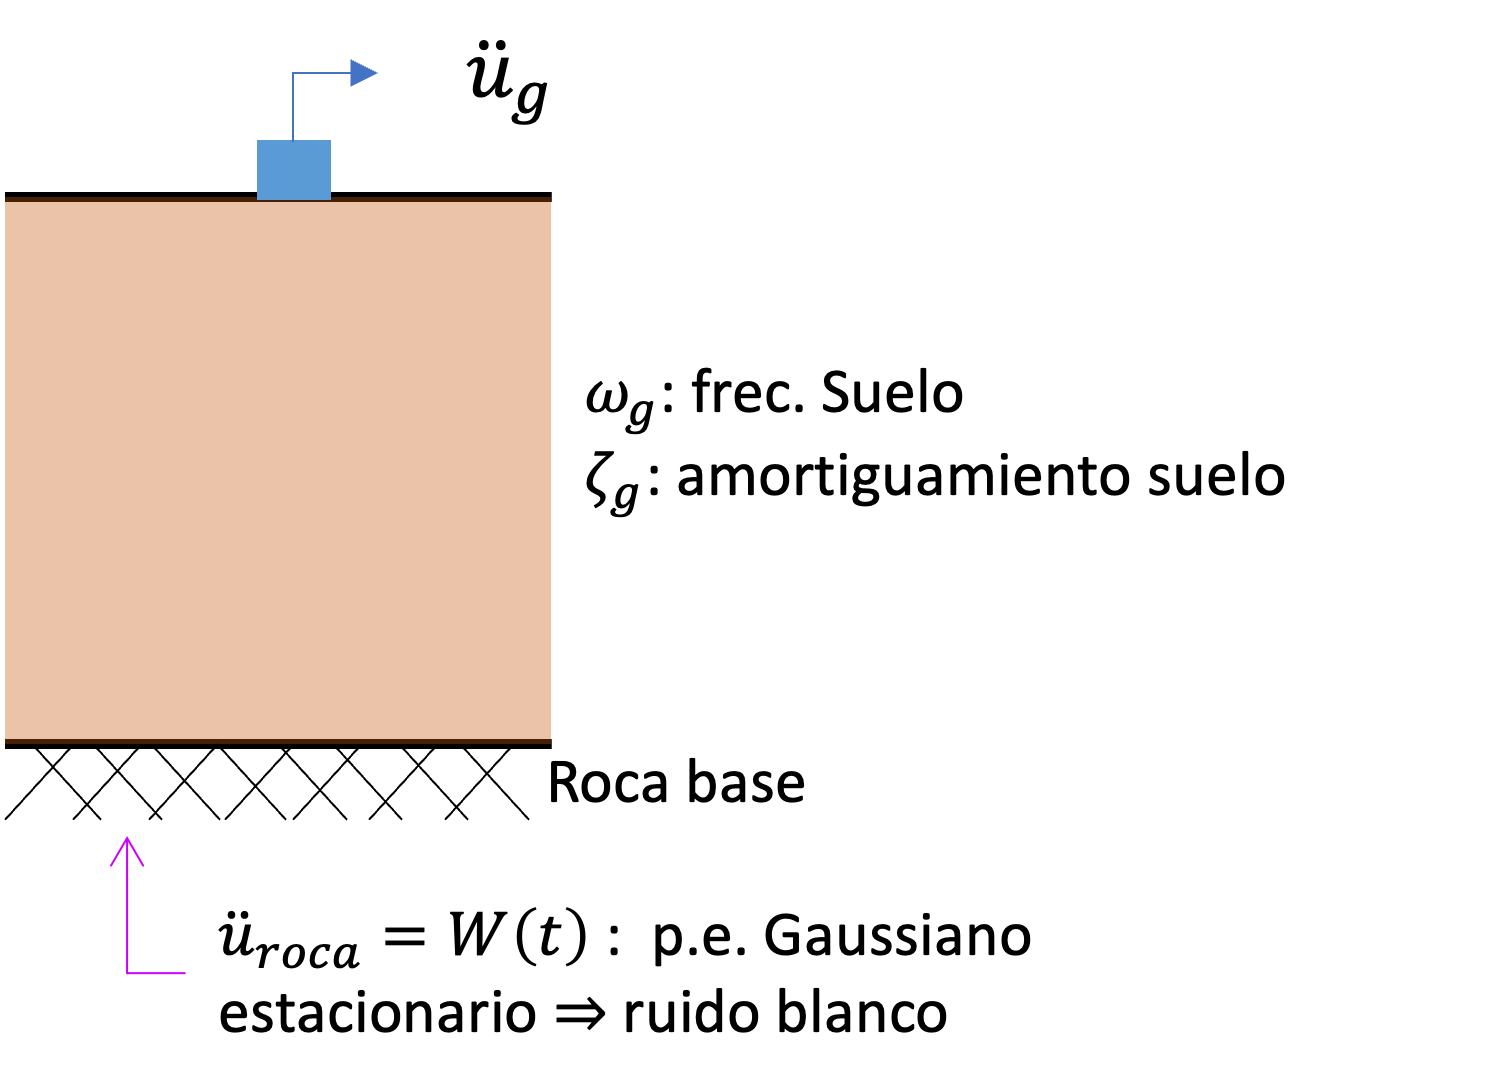
\includegraphics[scale=0.85]{Figuras/KT.png}
\end{figure}
EDM: $a$- estado del suelo
\begin{align*}
    \ddot{a}+2\xi_g\omega_g\dot{a}+\omega_g^2a=W(t) 
\end{align*}

Ruido blanco: 
$$\mathbb{E}\{W(t)\}=0$$ 
$$\mathbb{E}\{W(t)W(t+\tau)\}=2\pi S_0\delta(\tau)$$

$S_0$: poder espectral del sismo en roca (Intensidad del terremoto).\\

\par Ecuación de respuesta:
\begin{align*}
    \ddot{u}_g = -2\xi_g\omega_g \dot{a}-\omega_g^2a
\end{align*}
donde $\ddot{u}_g$ es la aceleración del suelo en campo libre.\\
\par Se puede demostrar que la función de respuesta en frecuencia (FRF) del estado de suelo es:

\begin{align*}
    H_{KT}(\Omega) &= \frac{\omega_g^2+i2\xi_g\omega_g\Omega}{(\omega_g^2-\Omega^2)+i2\xi_g\omega_g\Omega}\\
    |H_{KT}(\Omega)| &= \frac{\omega_g^4+4\xi_g^2\omega_g^2\Omega^2}{(\omega_g^2-\Omega^2)+4\xi_g^2\omega_g^2\Omega^2}
\end{align*}

\begin{figure}[H]
\centering
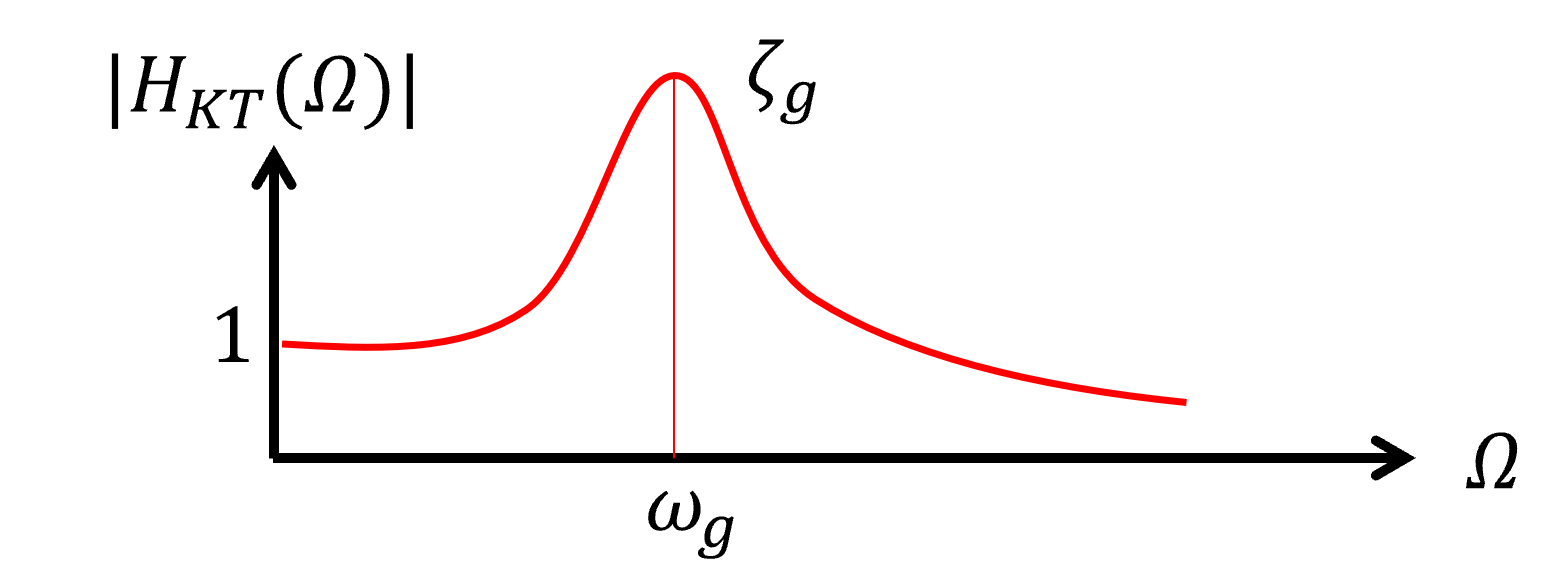
\includegraphics[scale=0.7]{Figuras/HKT.png}
\end{figure}


En espacio-estado:
\begin{align*}
    \dot{x}_g &= A_gx_g+B_gw(t), \quad x_g=a\\
    y_g &= C_gx_g, \quad y_g=\ddot{u}_g
\end{align*}

Diagrama de bloques:

\begin{figure}[H]
\centering
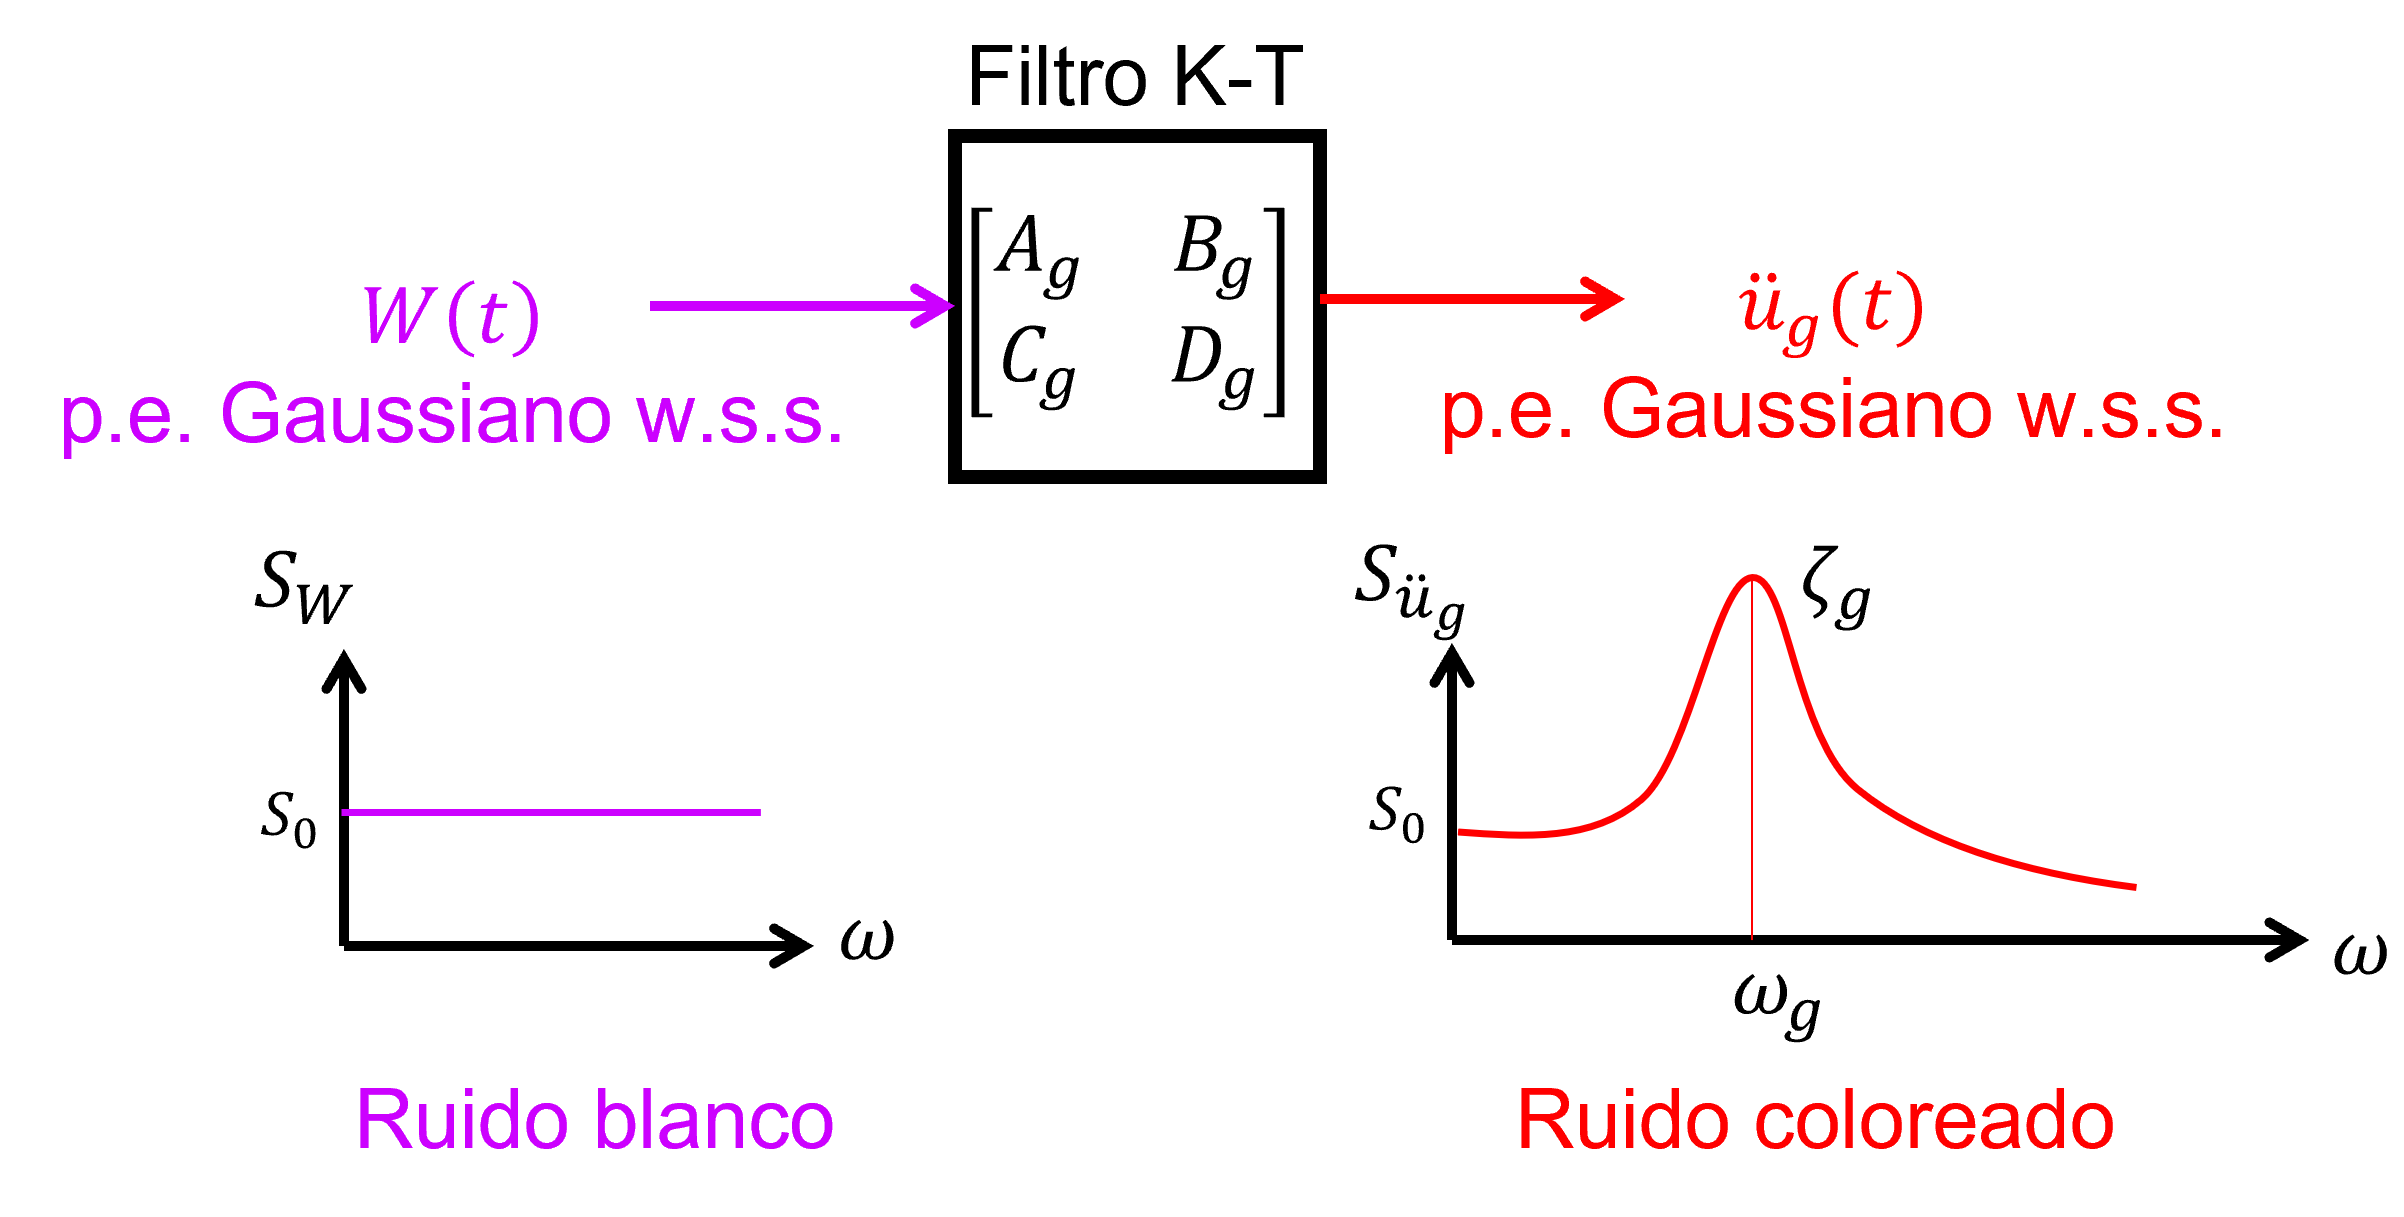
\includegraphics[scale=0.6]{Figuras/diagrama_bloque_KT.png}
\end{figure}

\begin{align*}
    \ddot{u}_g(t) &= h_{KT} \ast W(t)\\
    \ddot{u}_g(t)\ddot{u}_g(t+\tau) &= h_{KT}^2(t) \ast W(t)W(t+\tau)\\
    \Longrightarrow s_{\ddot{u}_g}(\omega) &= |H_{KT}(\omega)|^2s_0
\end{align*}

Parámetros del modelo K-T: $s_0$, $\omega_g$, $\xi_g$.\\
\par Terremoto El Centro (1940): 
\begin{itemize}
    \item $\bar{\omega}_g = 18$ rad/s
    \item $\bar{\xi}_g = 0.60$
    \item $s_0 = $ depende del peak ground acceleration (PGA)
\end{itemize}

En estado estacionario:

\begin{figure}[H]
\centering
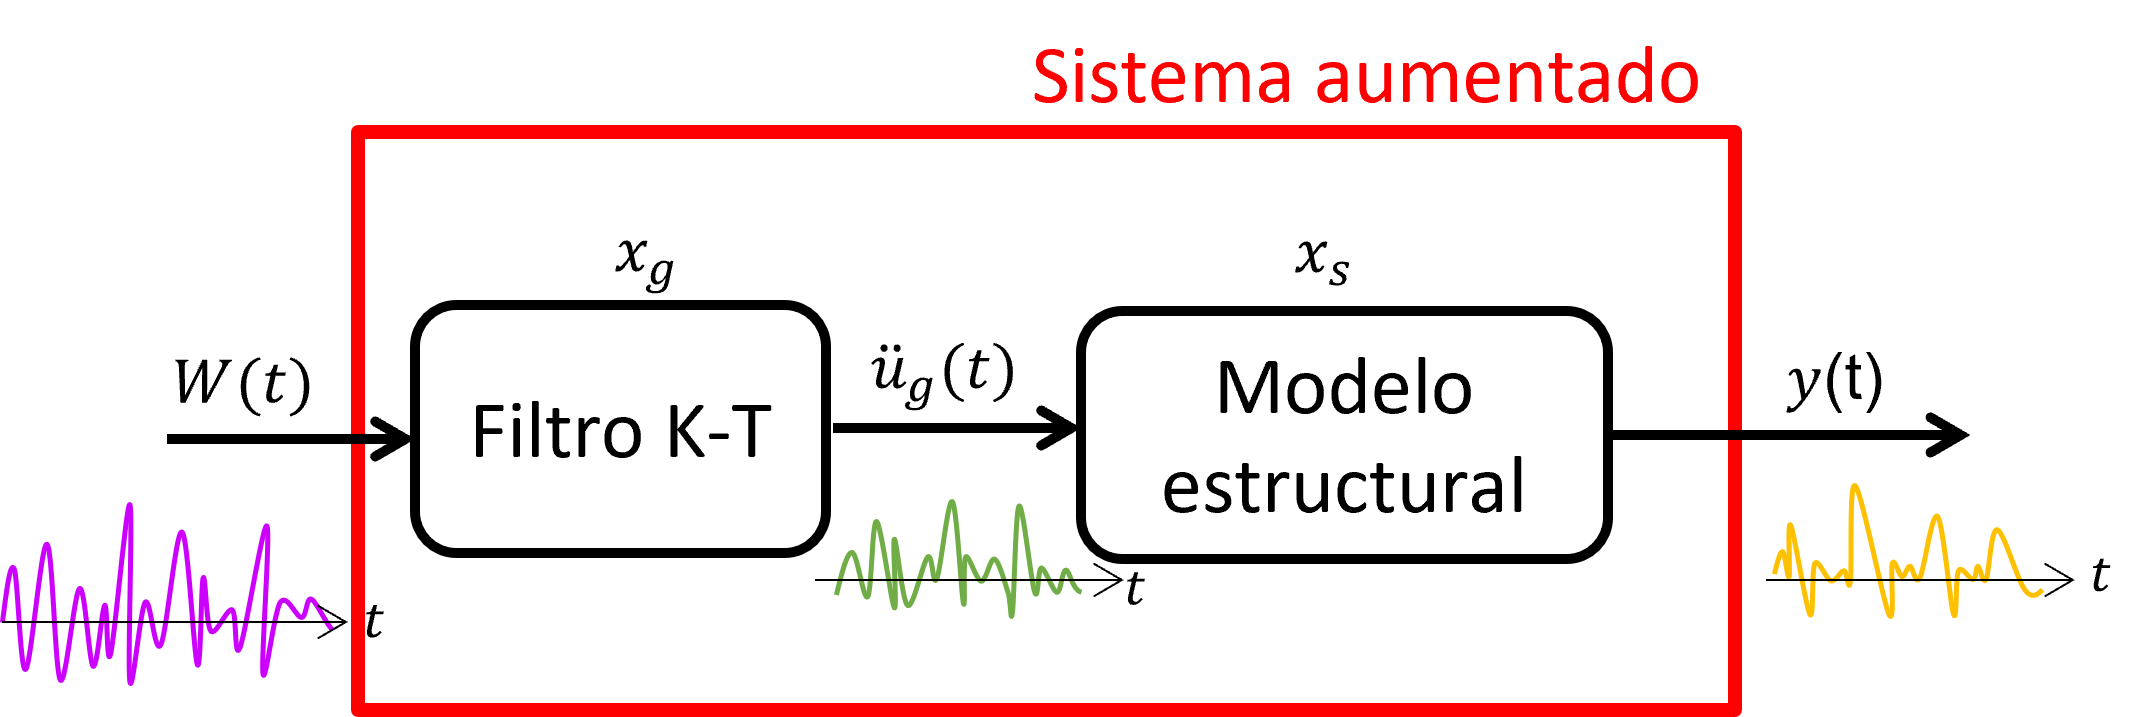
\includegraphics[scale=0.7]{Figuras/estado_estacionario_KT.png}
\end{figure}
Estados: $x_a=\left\{
    \begin{array}{c}
     x_s \\ x_g 
    \end{array}\right\}$
\begin{align*}
    \dot{x}_a&=A_ax_a+B_aW(t)\\
    y &= C_ax_a
\end{align*}

\par Ec. de Lyapunov:
\begin{align*}
    0 &= A_x\Gamma_x +\Gamma_aA_a^\top+Q_a\\
    \Gamma_a &= \mathbb{E}\{x_ax_a^\top\}\\
    \Gamma_y &= C_a\Gamma_aC_a^\top \Longrightarrow \text{RMS respuesta}
\end{align*}

Pero, en realidad los registros sísmicos son p.e. no estacionarios:

\par ¿Podemos ocupar K-T? $\longrightarrow$ Sí, a través de una \textcolor{red}{función de modulación}\\

\begin{figure}[H]
\centering
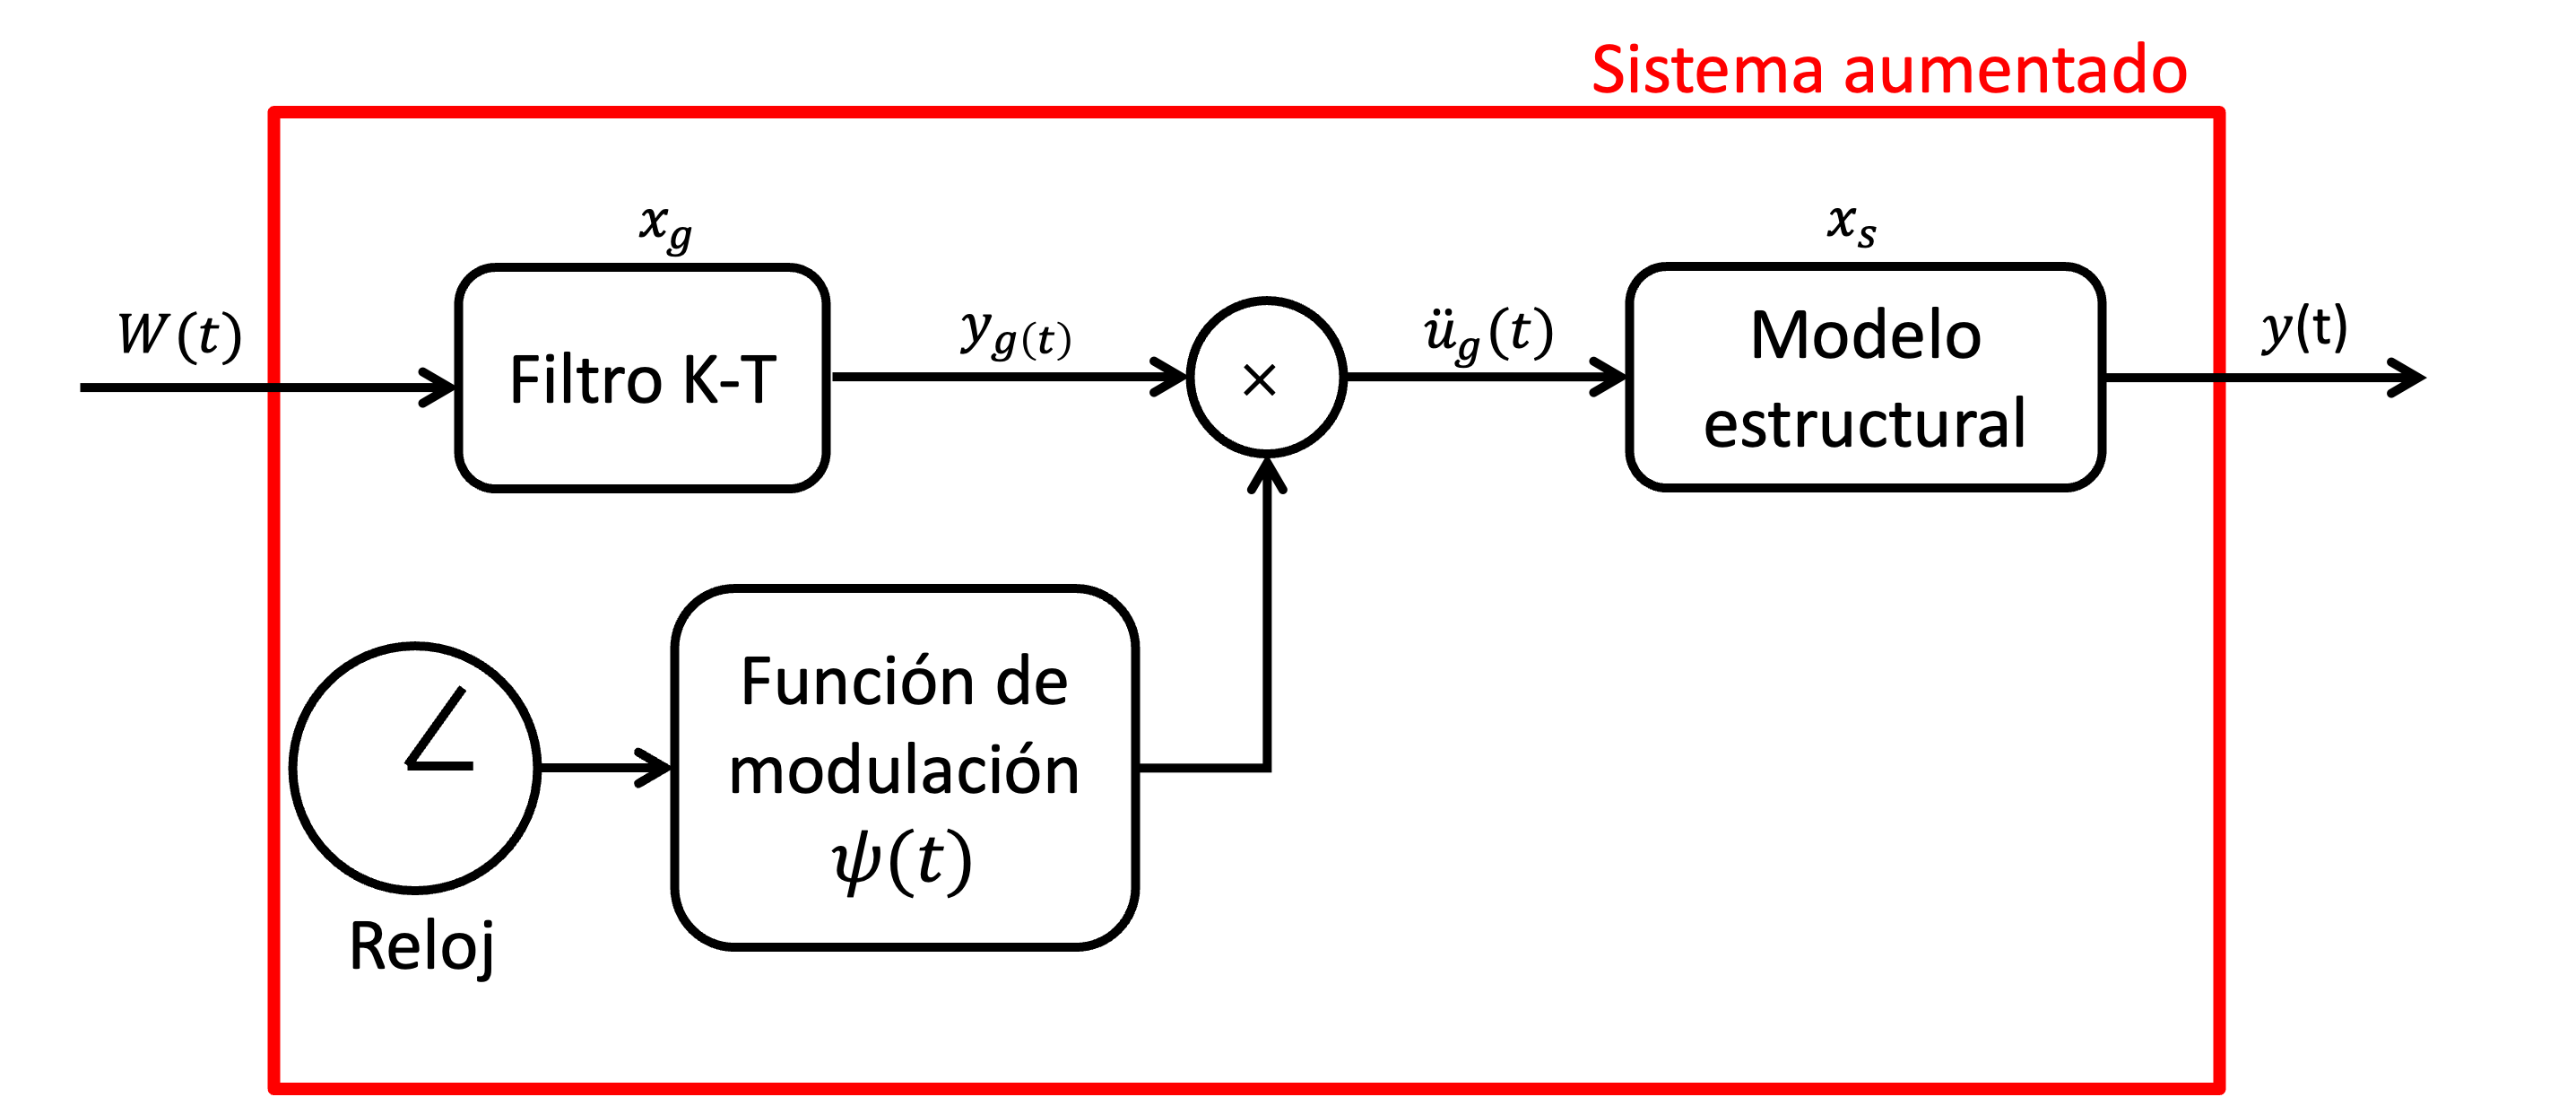
\includegraphics[scale=0.6]{Figuras/func_mod_KT.png}
\end{figure}
\begin{figure}[H]
\centering
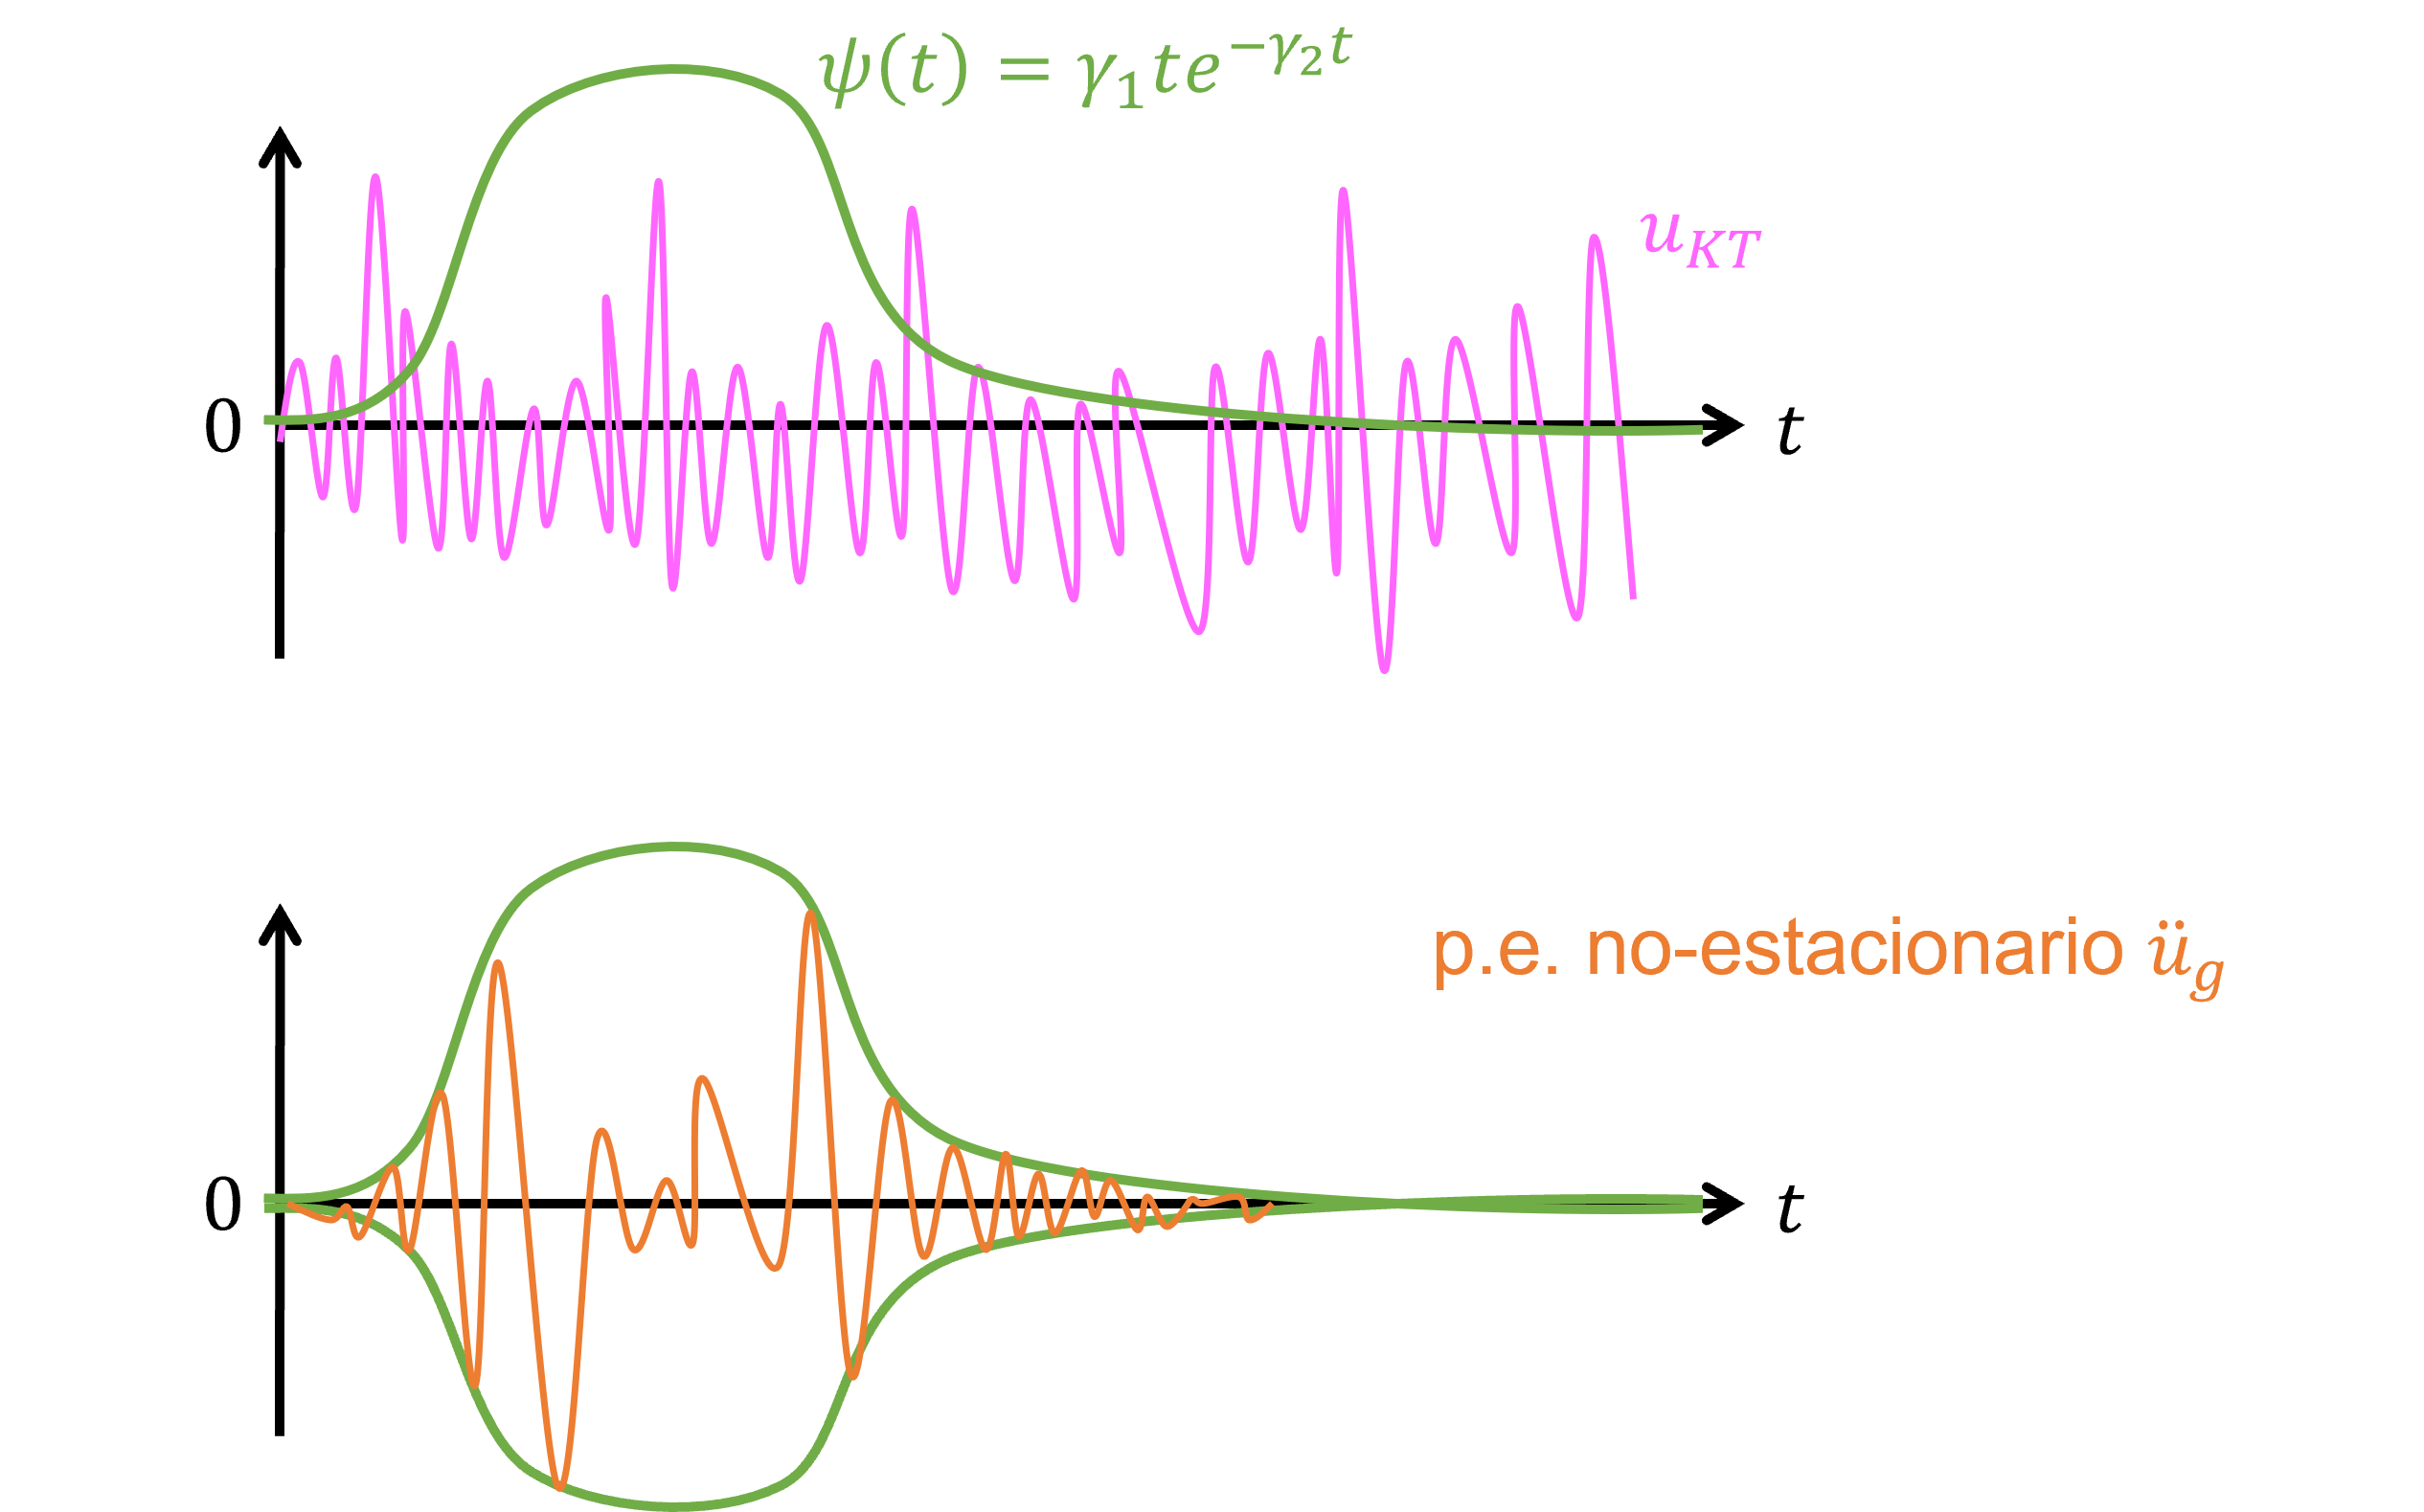
\includegraphics[scale=0.6]{Figuras/func_mod_KT2.png}
\end{figure}

\par Sistema atenuado (LTV): 
\begin{align*}
    \dot{x}_a(t) &= A_a(T)x_a(t)+B_a(t)Z(t)\\
    y(t) &= C_a(t)x_a(t)
\end{align*}
$\Longrightarrow$ Ec. diferencial de Lyapunov:
\begin{align*}
    \dot{\Gamma}_a(t) = A_a(t)\Gamma_a(t)+\Gamma_a(t)A_a^\top (t))+Q_a(t)
\end{align*}

Integrar, resolver $\Gamma_a(T)\Longrightarrow \Gamma_y (t) \Longrightarrow\text{rms } y(t)$.




\chapter{Procesamiento Digital de Señales}

\section{Sistemas discretos}

Es necesario convertir una señal análoga a discreta.

\begin{figure}[H]
    \centering
    
\includegraphics[scale=0.7]{Figuras/sist_discreto.png}
\end{figure}

Razón: Queremos realizar calculos de la señal en un computador.

\begin{figure}[H]
    \centering
    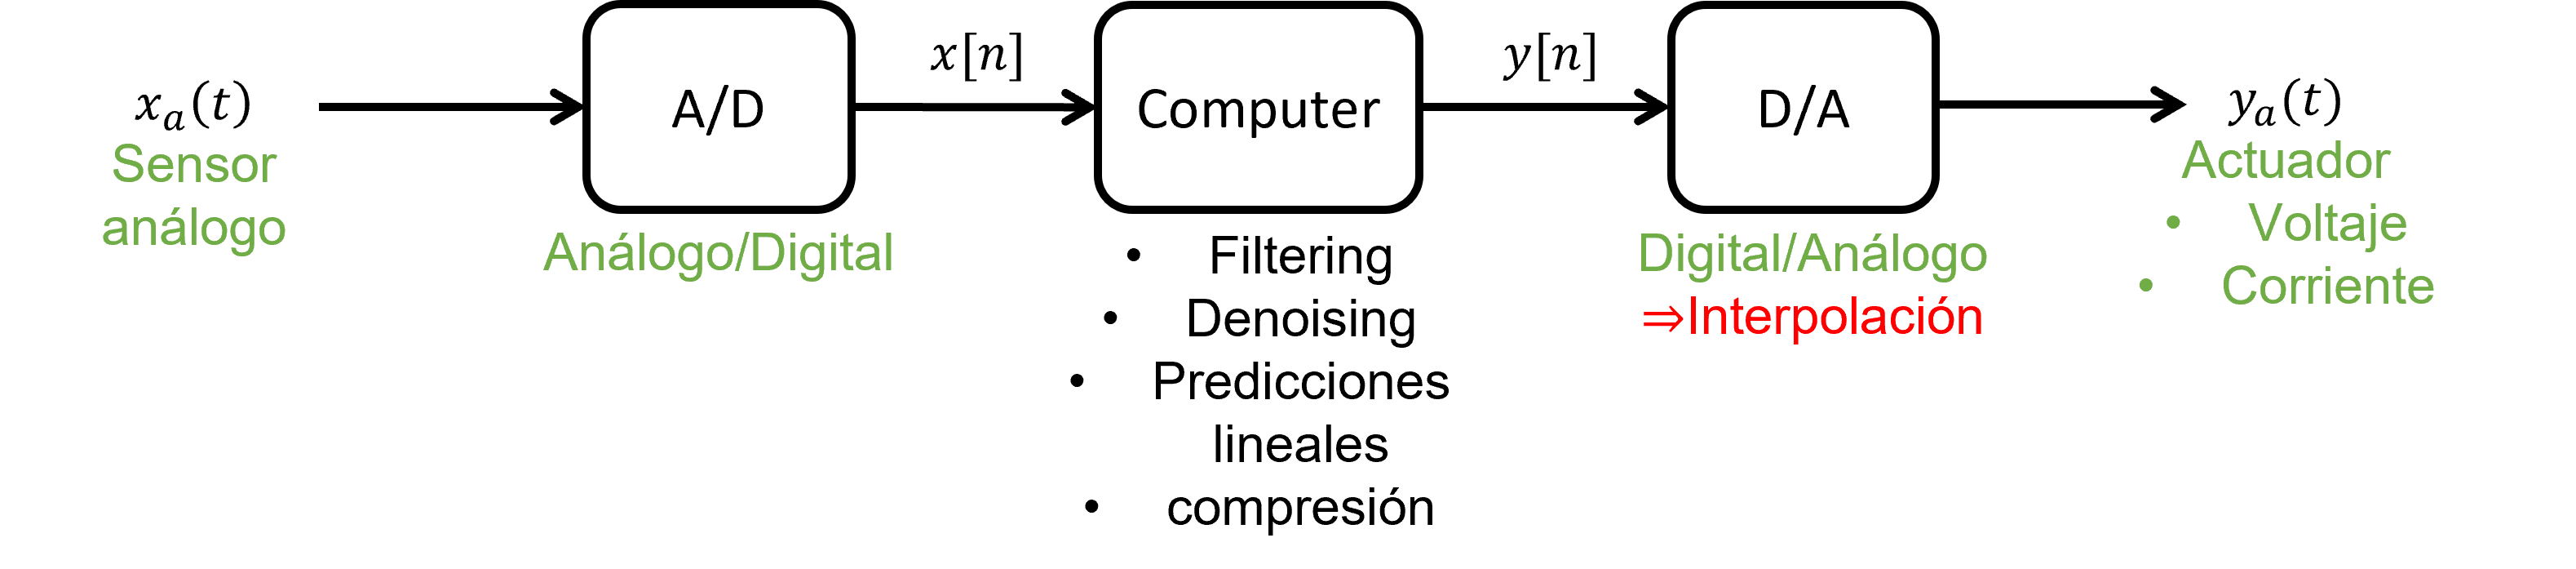
\includegraphics[scale=0.7]{Figuras/sistema_discret.png}
\end{figure}

\subsection{Muestreo}

\begin{enumerate}
    \item Muestreo en el tiempo $\Longrightarrow$ Sampling
    \item Muestreo en amplitud $\Longrightarrow$ Quantization
\end{enumerate}

\subsection{Cuantización}

En el contexto de la conversión analógica a digital (ADC, Analog-to-Digital Conversion), la cuantización (quantization) es el proceso mediante el cual se convierte un valor analógico continuo en un valor digital discreto.

Por ejemplo, una máquina 8 bits $\Longrightarrow$ Números utilizando $2^{8}$ cifras significativas.

\begin{align*}
    \text{Bit} = \left\{ \begin{array}{l}
             0 \\
             1
             \end{array}
   \right. \Longrightarrow 256 \text{ niveles}
\end{align*}

Durante la cuantización, cada valor analógico medido se aproxima al nivel más cercano de entre esos 256 niveles.

Por ejemplo, si el rango es $0 - 5$ V, cada nivel representa un salto de $\Delta = 5/256 \approx 0.0195$ V. Si el valor analógico real es $1.23$ V, el ADC lo “cuantiza” al nivel más cercano, por ejemplo $1.22$ V.

Esta aproximación introduce un error de cuantización, que es la diferencia entre el valor analógico real y el valor cuantizado. Este error es inevitable y depende de la resolución del ADC: a mayor número de bits, menor error de cuantización.

\underline{Nota}: Computadores representan números utilizando dígitos binarios (bits almacenados en flip-flops).\\

\subsection{Señal en tiempo discreto}

\begin{figure}[H]
    \centering
    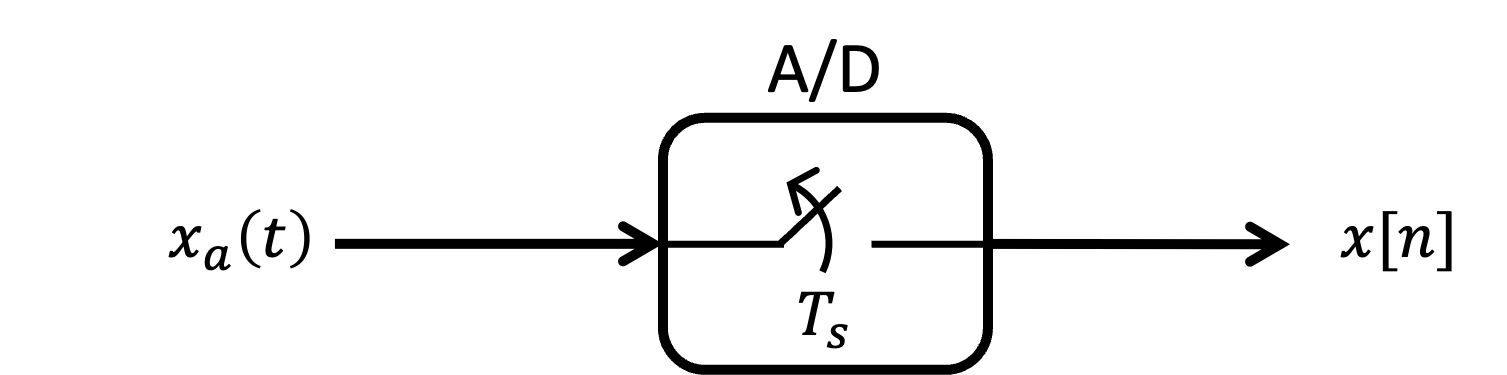
\includegraphics[scale=0.7]{Figuras/AD.png}
\end{figure}


\begin{align*}
    x[n]=x_a(nT_s)
\end{align*}

\noindent donde $x[n]$ es la señal en tiempo discreto, $T_s$ es el paso temporal de muestreo, y $n$ es el índice temporal (número entero).\\

\begin{figure}[H]
    \centering
    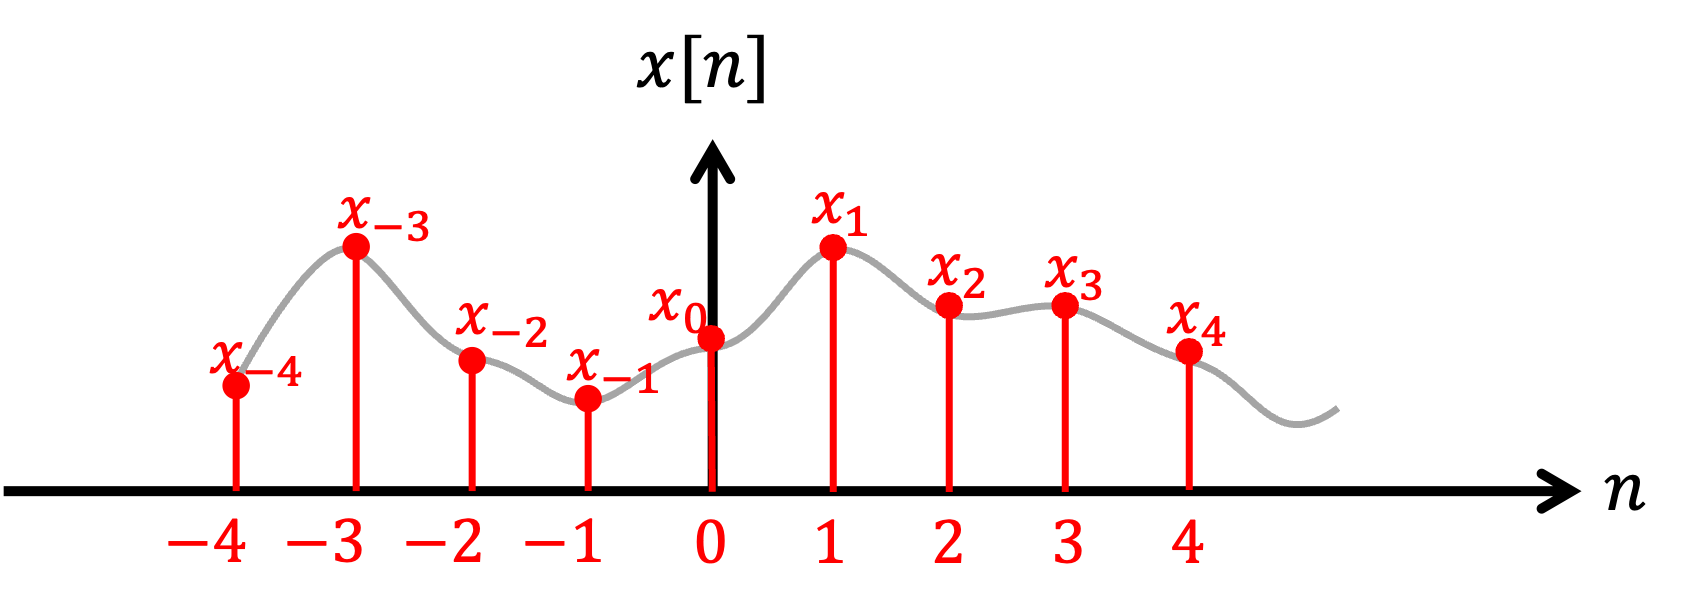
\includegraphics[width=4in]{Figuras/senaldiscreta.png}
\end{figure}

La representación matemática del muestreo se puede realizar utilizando la \underline{Función pulso unitario}:

\begin{figure}[H]
    \centering
    
\includegraphics[scale=0.7]{Figuras/pulso_unitario.png}
\end{figure}

\begin{align*}
    \delta[n] = 
    \begin{cases}
        1, & n=0\\
        0,& n \neq 0
    \end{cases}
\end{align*}

\begin{align*}
    x[n]=\sum_{k=0}^{N-1} x_k \delta[n-k]=x_0\delta[n]+x_1\delta[n-1]+x_2\delta[n-2]+...+x_{N-1}\delta[n-(N-1)]
\end{align*}

\begin{align*}
    \{x_n\}_0^{N-1}=\{x_0,x_1,x_2,...,x_{N-1}\} \Longrightarrow \text{Arreglo de N puntos (vector)}
\end{align*}


\section{Análisis en frecuencia}

\begin{figure}[H]
    \centering
    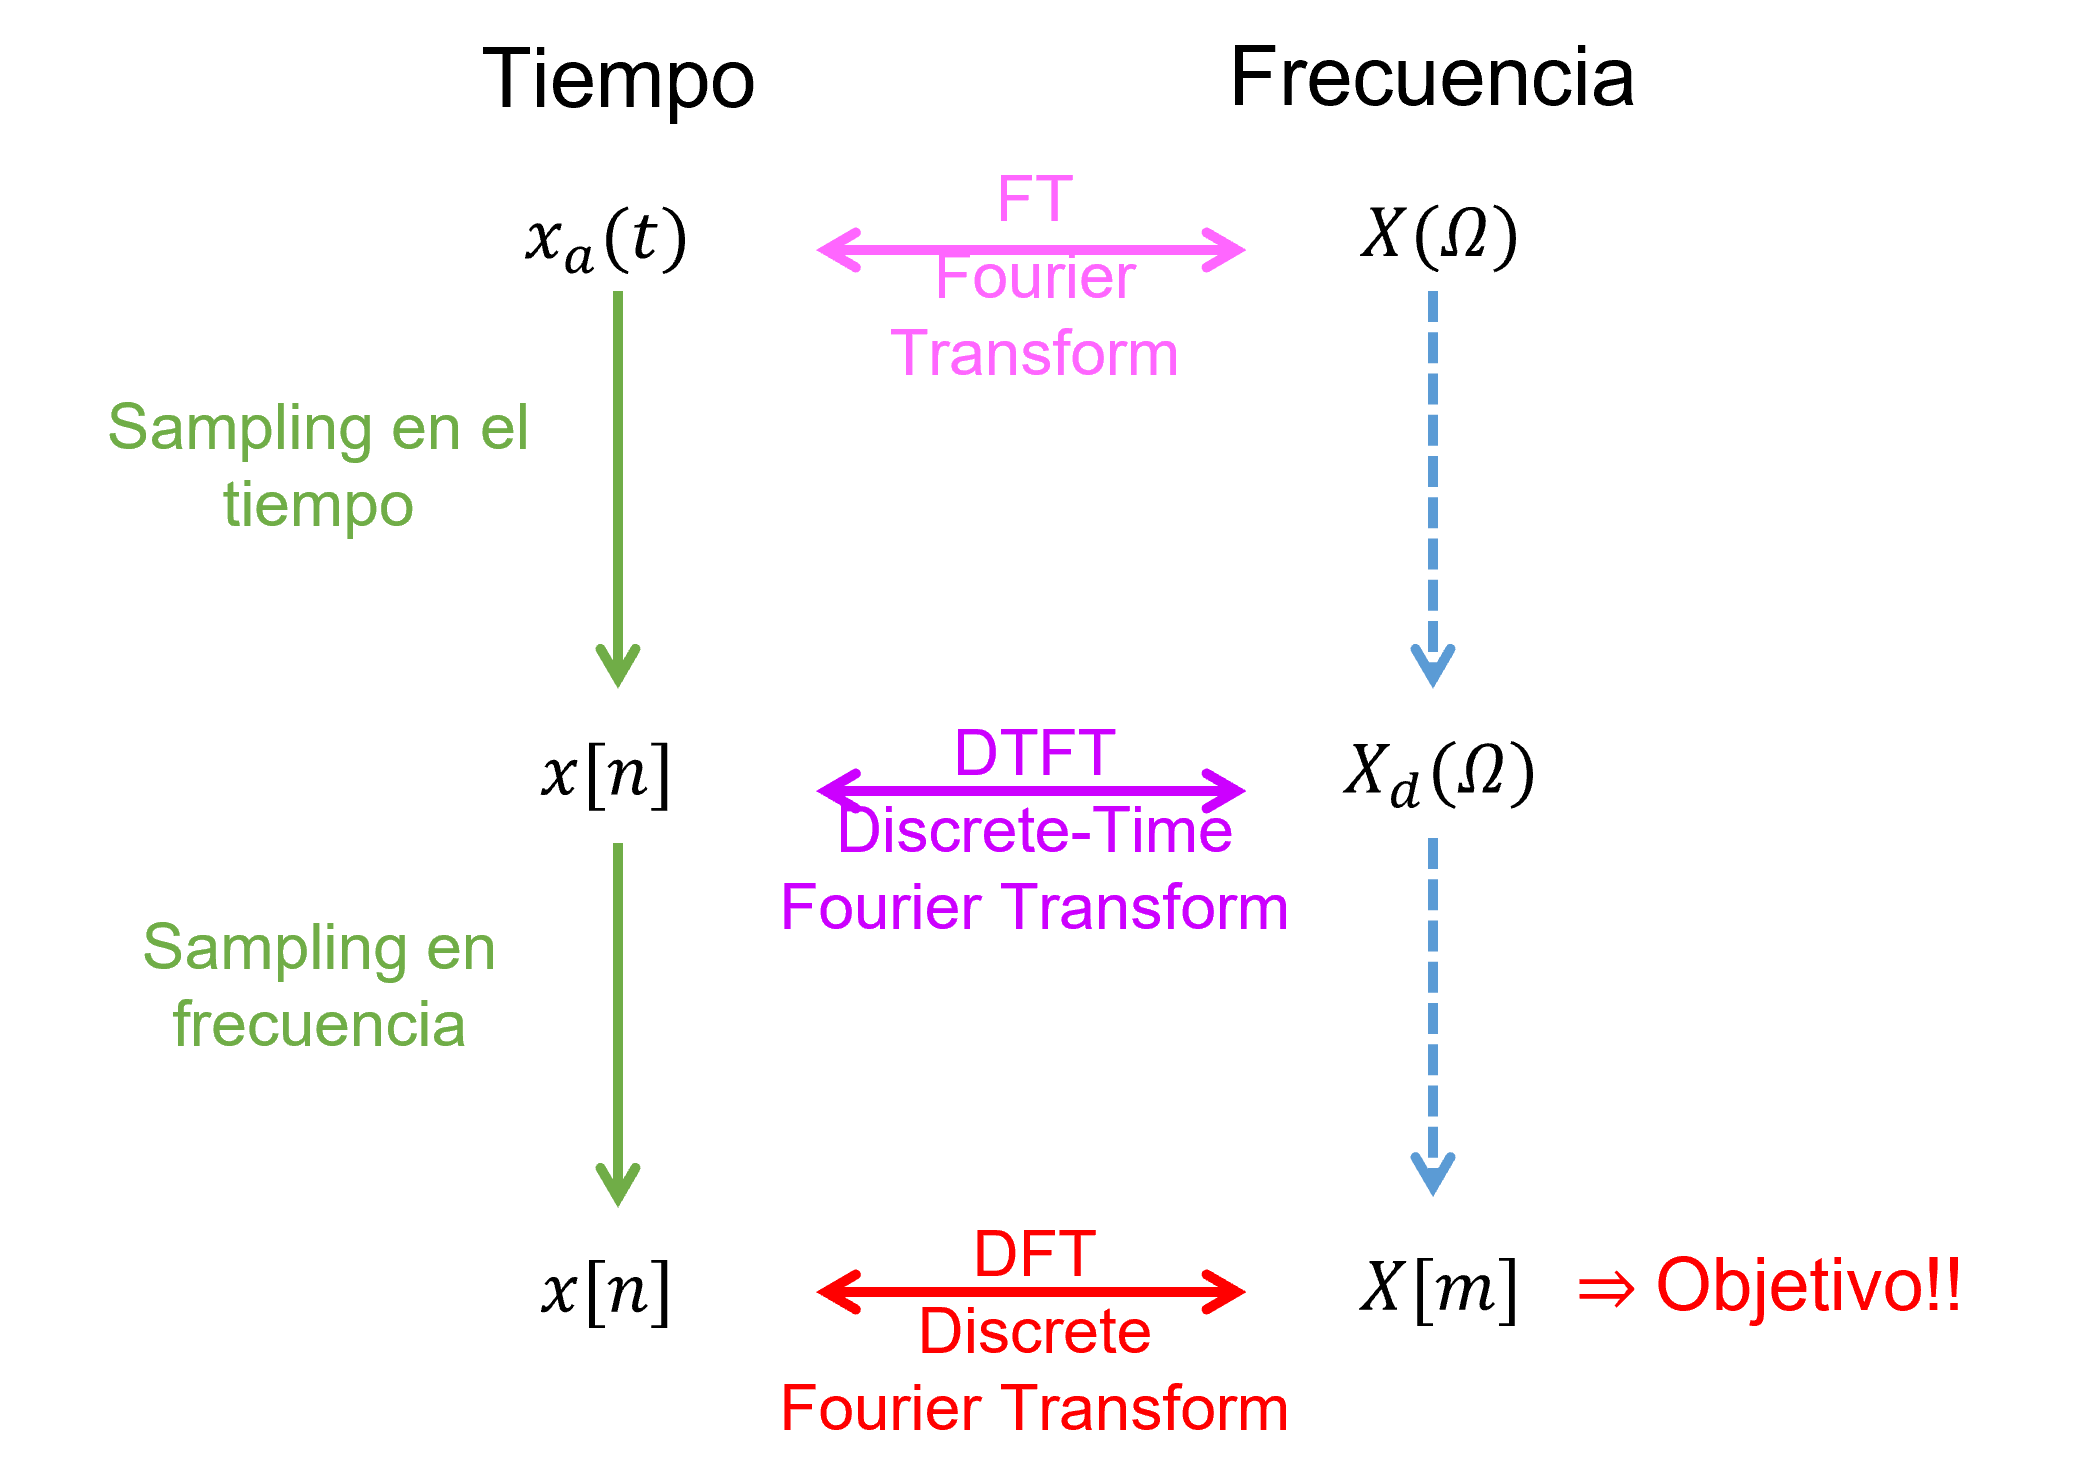
\includegraphics[scale=0.7]{Figuras/analisis_frec.png}
\end{figure}

\noindent \emph{Nota:} $j = \sqrt{-1}$ es el número complejo.\\

\subsection{Continuous-Time Fourier Transform (CTFT)}

\begin{align*}
    X(\Omega) &= \int_{-\infty}^{+\infty}x_a(t)e^{-j\Omega t}dt \quad \text{(CTFT)}\\
    x_a(t) &= \frac{1}{2\pi}\int_{-\infty}^{+\infty}X(\Omega)e^{+j\Omega t}d\Omega \quad \text{(inverse CTFT)}
\end{align*}

$t, \Omega \in \mathbb{R}$, $x_a(t)\in \mathbb{R}$, $X(\Omega)\in \mathbb{C}$\\

\subsection{Discrete-time Fourier Transform (DTFT)}

Supongamos que la señal $x(t)$ es discretizada en el tiempo, $x[n] = x(n T_s)$, donde $T_s$ es el período de muestreo. Entonces, el DTFT se define:

\begin{align*}
    X_d(\omega) &= \sum_{n=-\infty}^{\infty}x[n]e^{-j\omega n} \quad \text{(DTFT)}\\
    x[n] &= \frac{1}{2\pi}\int_{-\infty}^{\infty}X_d(\omega)e^{+j\omega n}d\omega \quad \text{(inverse DTFT)}
\end{align*}

donde $\omega \in \mathbb{R}$, $n \in \mathbb{Z}$.

\subsection{Discrete Fourier Transform (DFT)}

La DFT opera sobre una secuencia de $N$ puntos en tiempo, $x[n], n \in \{0,1,2,\ldots,N-1\}$, y produce una secuencia de $N$ puntos en frecuencia, $X[m], m \in \{0,1,2,\ldots,N-1\}$.

\begin{align*}
    X[m] &= \sum_{n=0}^{N-1} x_ne^{-j\frac{2\pi}{N}nm} \quad \text{(DFT)}\\
    x[n] &= \frac{1}{N}\sum_{m=0}^{N-1}X_me^{+j\frac{2\pi}{N}nm} \quad \text{(Inverse DFT)}
\end{align*}

donde $n,m \in \{0,1,2,\ldots,N-1\}$.\\

\emph{Nota 1}: Se asume que la secuencia $x[n]$ es periódica.\\

\emph{Nota 2}: Fast Fourier Transform (FFT) es un algoritmo computacional para calcular el DFT.\\

\subsection{Relación entre DFT y DTFT}

\begin{align*}
    X[m]=X_d(\omega)\bigg|_{\omega=\frac{2\pi}{N}m}
\end{align*}

\subsection{Relación entre DTFT y CTFT}

\begin{align*}
    X_d(\omega) = \frac{1}{T} \sum_{l=-\infty}^{+\infty} X \left(\underbrace{\frac{\omega + 2\pi l}{T}}_{= \Omega} \right)
\end{align*}

\section{Criterio de muestreo de Nyquist}

En DSP, queremos muestrear la señal sin pérdida de información (``lossless''). Entonces, hay que elegir correctamente el intervalo de muestreo $T_s$ (sampling time).\\

\begin{theorem}[Teorema de Nyquist]
    La frecuencia de muestreo de una señal digital debe ser al menos el doble de la máxima frecuencia de la señal análoga:
    $$F_s > 2 f_{\max}$$
\end{theorem}

\section{Aliasing}

Aliasing es un fenómeno que ocure cuando el terorema de Nyquist no se cumple, es decir, $F_s \leq 2 f_{\max}$. Ocurre cuando una señal análoga no puede ser reconstruida por la señal digitalizada.\\

\underline{Ejemplo}: Video del ``helicoptero mágico'' \url{https://www.chrisfay.de/helicopter-video}. 

\subsection{Aliasing en dominio del tiempo}

\begin{figure}[H]
    \centering
    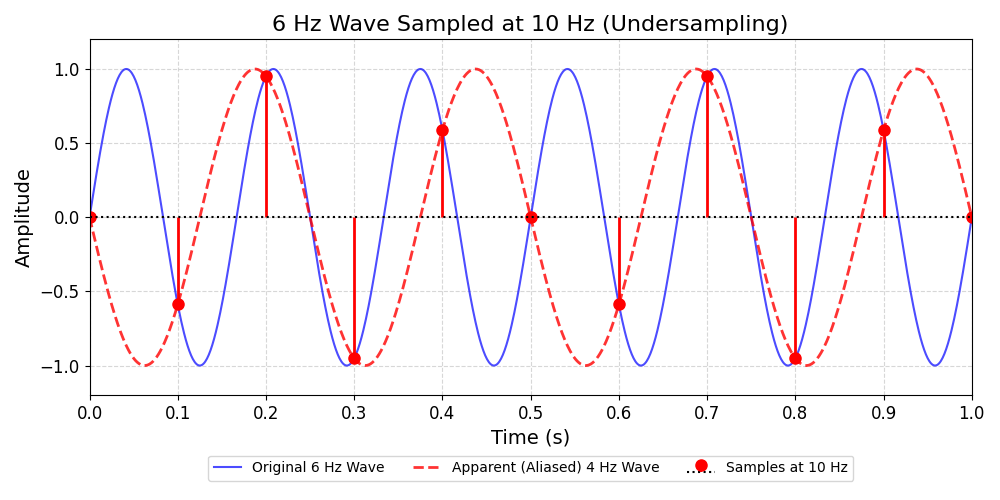
\includegraphics[width=6in]{Figuras/AliasingTimeExample.png}
\end{figure}

\subsection{Aliasing en dominio de frecuencia}

\begin{figure}[H]
    \centering
    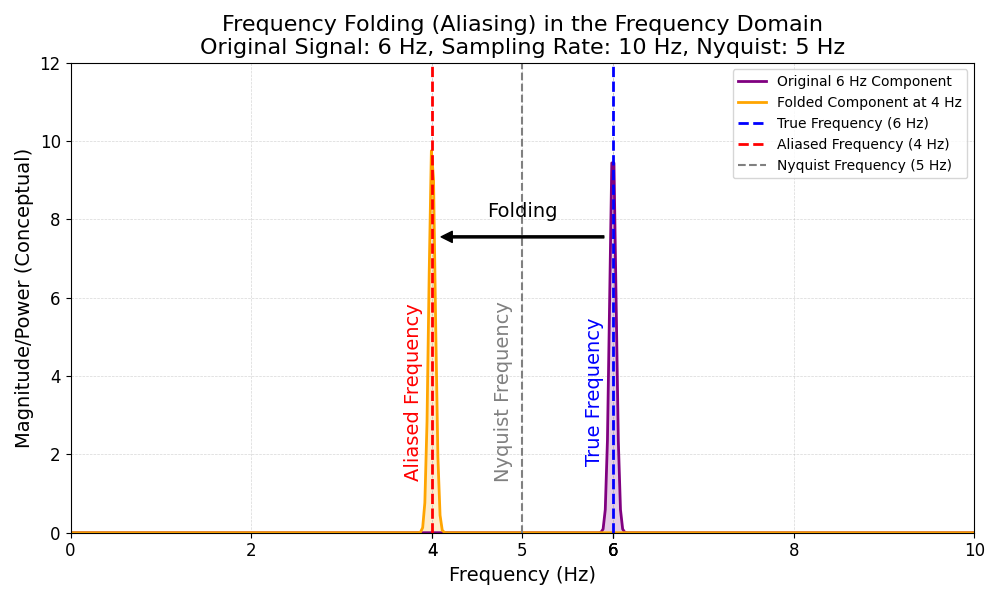
\includegraphics[width=6in]{Figuras/aliasing_frequency_folding.png}
\end{figure}

Considere $f = 2 \pi \Omega$, donde $f$ es frecuencia [Hz] y $\Omega$ es frecuencia (cicular) [rad/s].

\subsubsection{Sin Aliasing}

\begin{figure}[H]
\centering
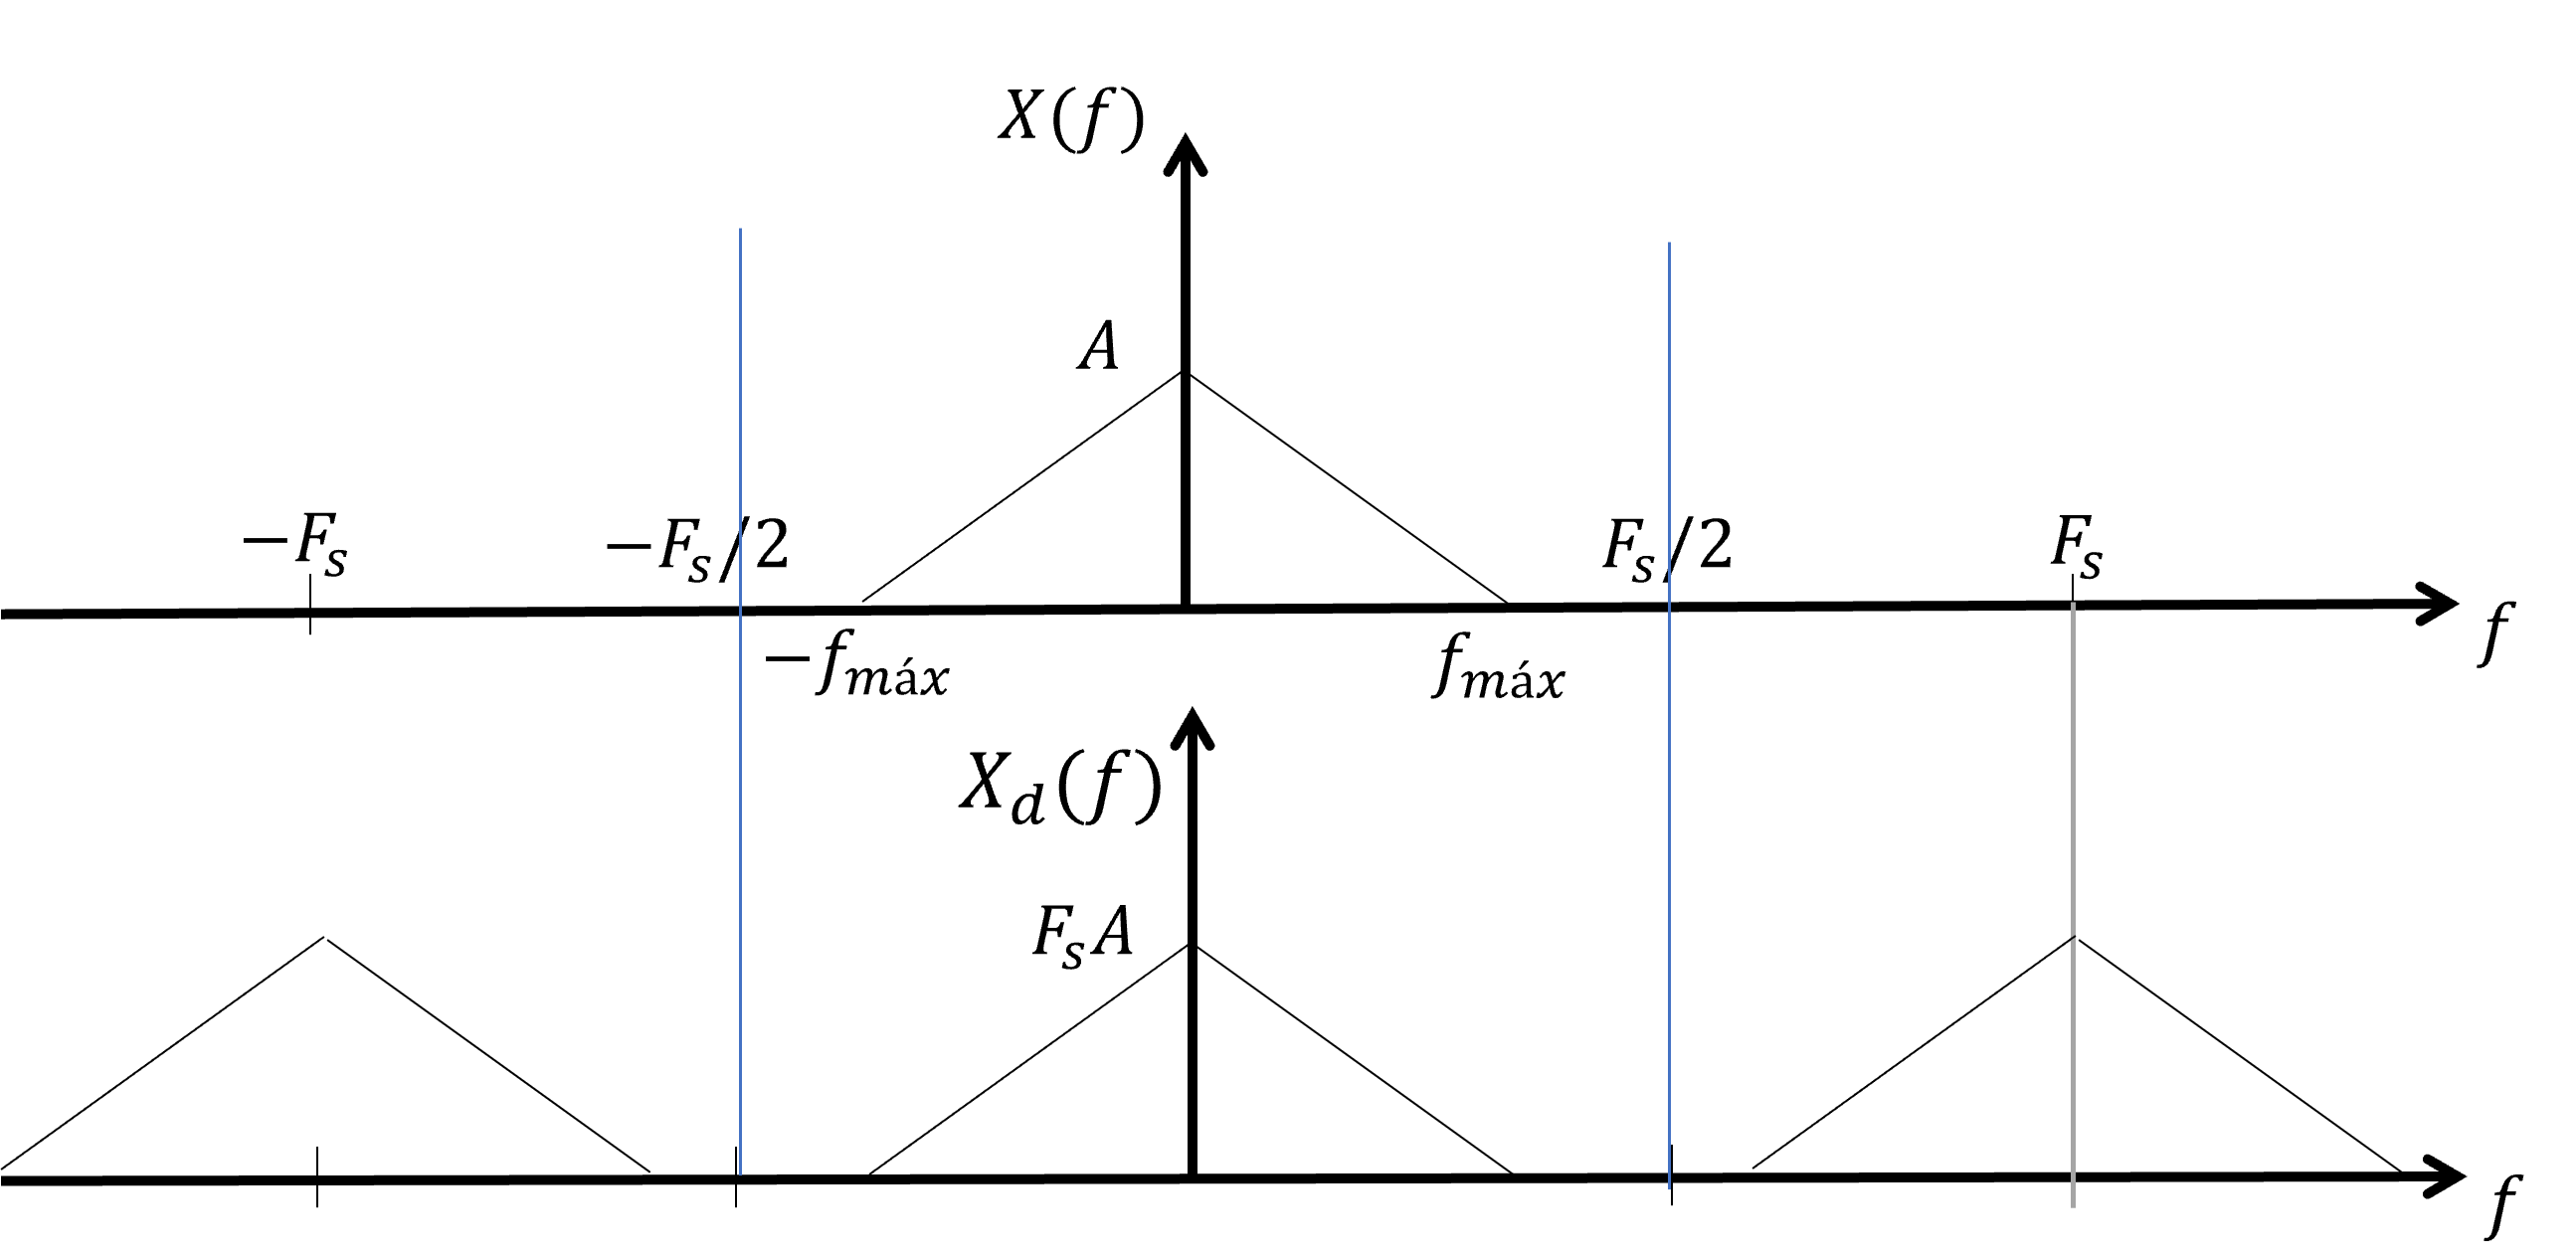
\includegraphics[scale=0.7]{Figuras/sin_aliasing.png}
\end{figure}

\begin{align*}
    F_s &> 2f_{max}\\
    f_{max} &< \frac{F_s}{2}=F_N \quad \text{(frecuencia de Nyquist)}
\end{align*}

\subsubsection{Con Aliasing}

\begin{figure}[H]
\centering
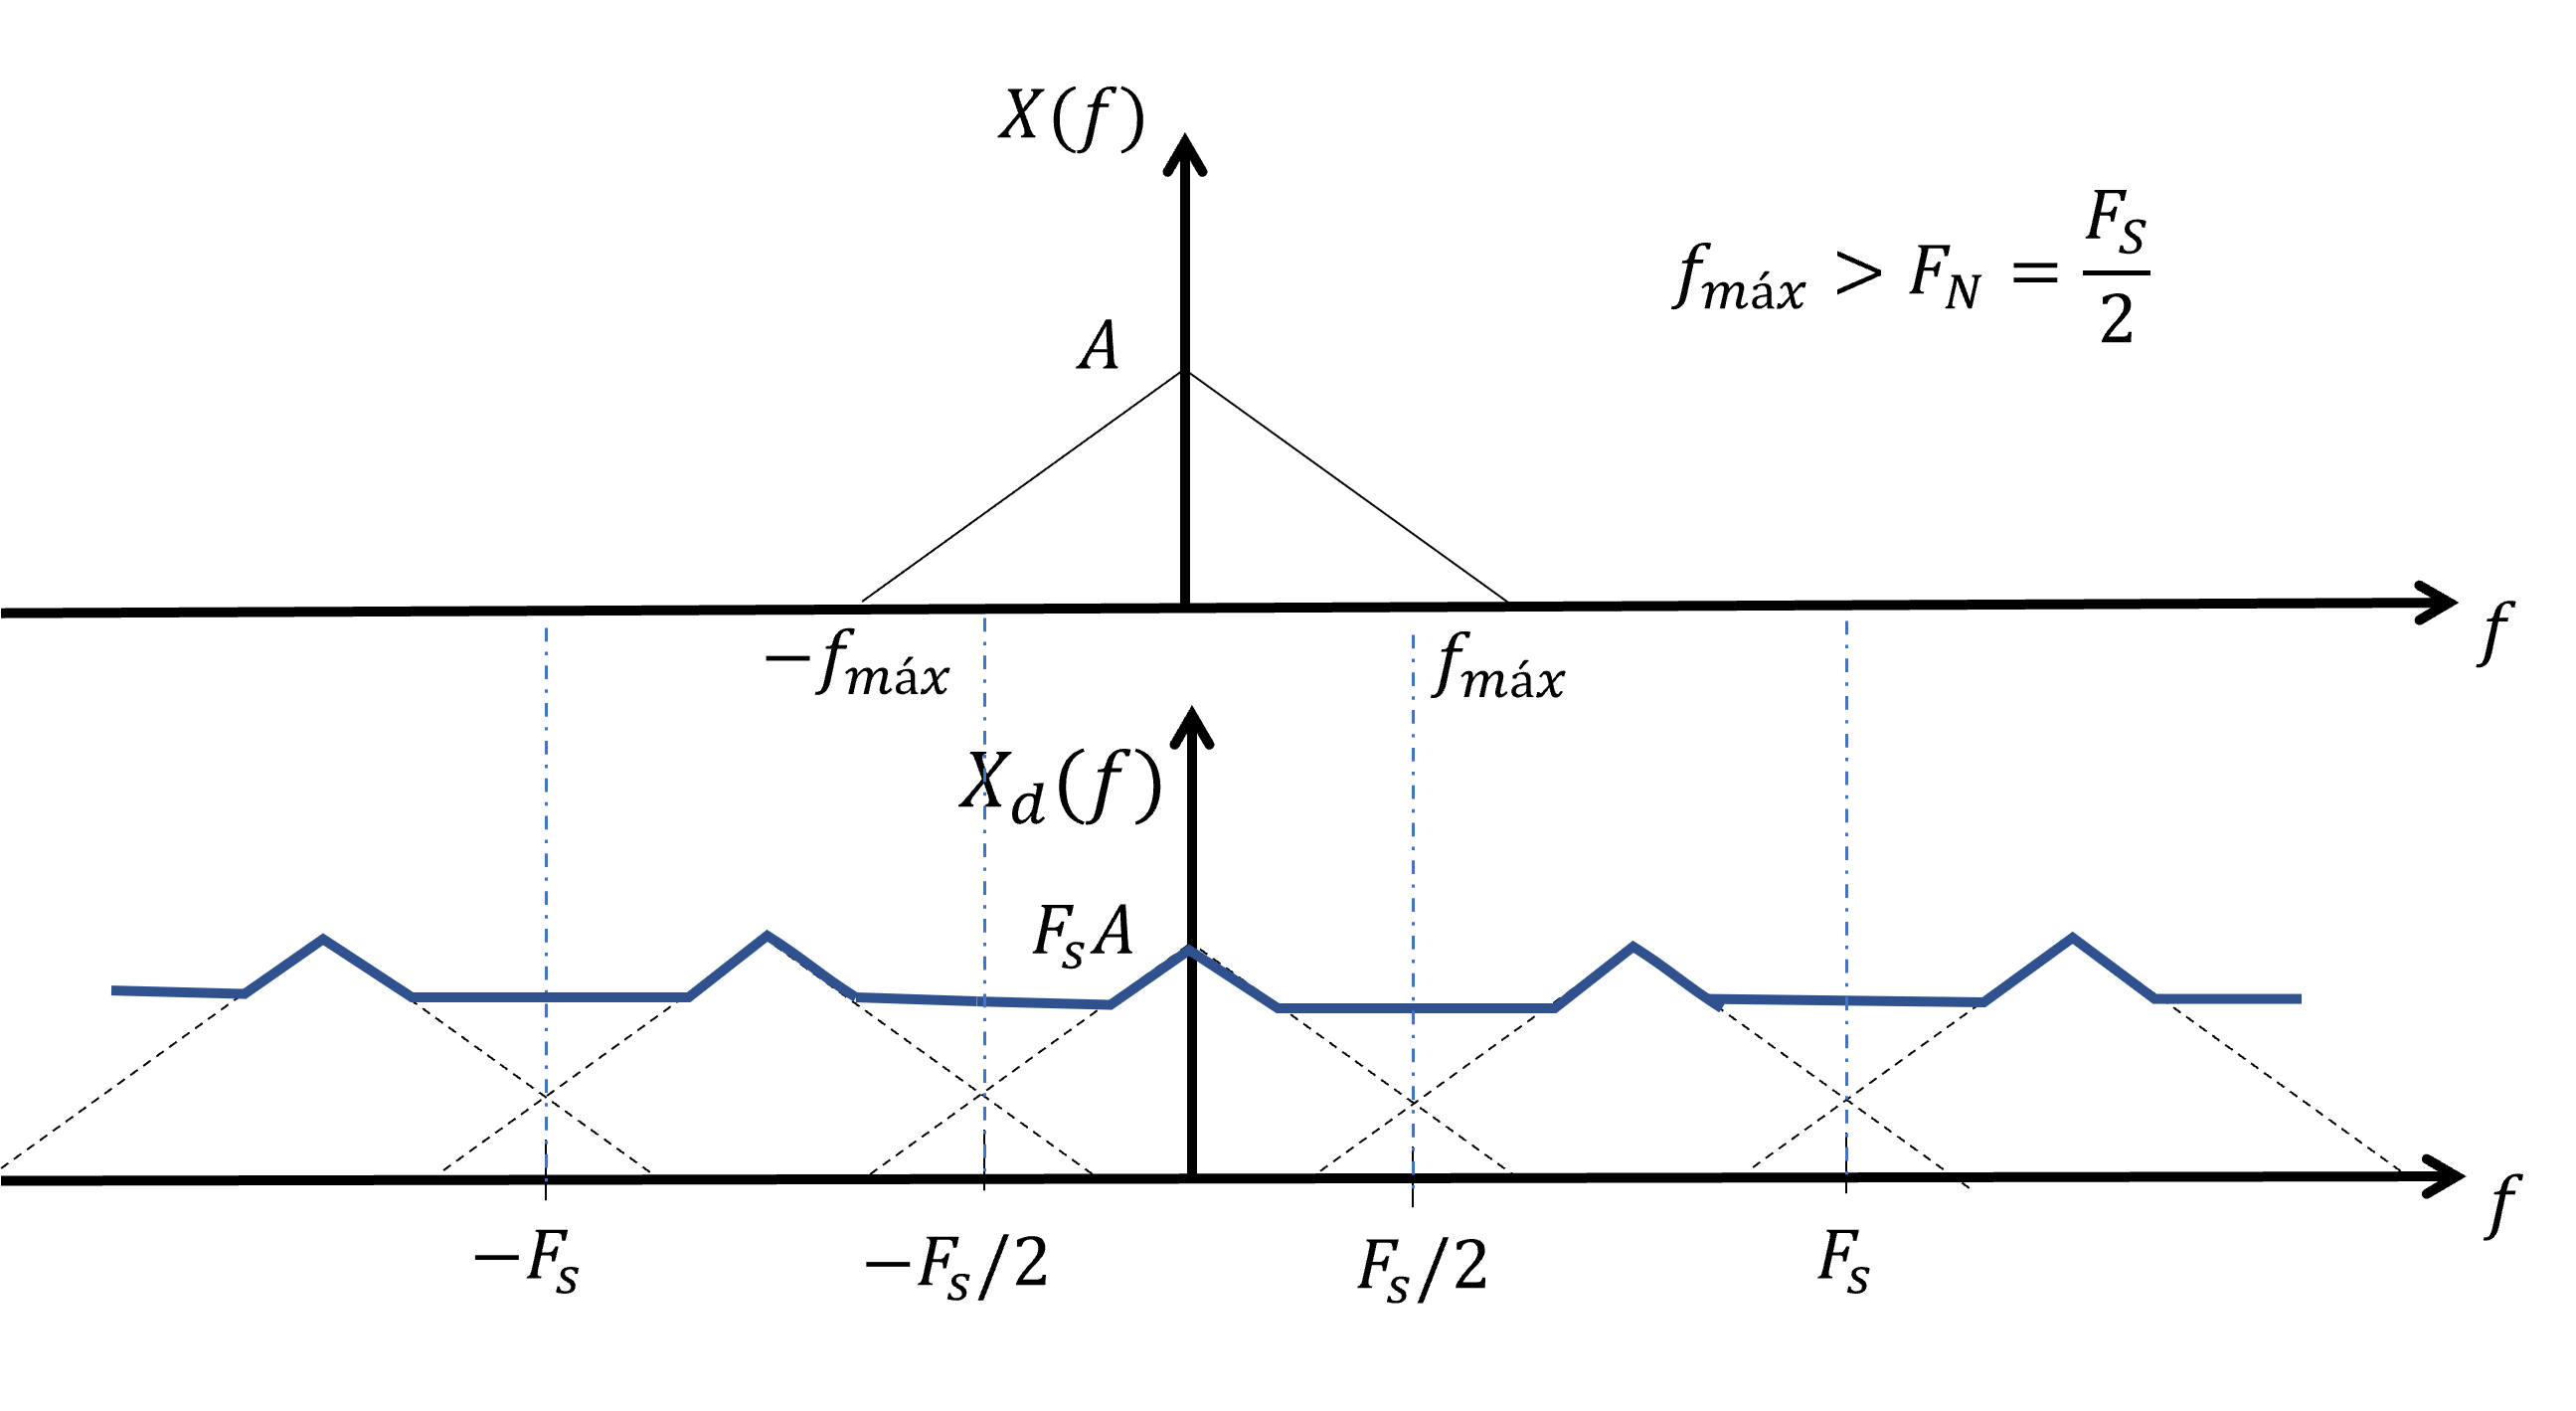
\includegraphics[scale=0.7]{Figuras/con_aliasing.png}
\end{figure}

Ejemplo: PSD de respuesta estructural de un sistema 3DOF

\begin{figure}[H]
\centering
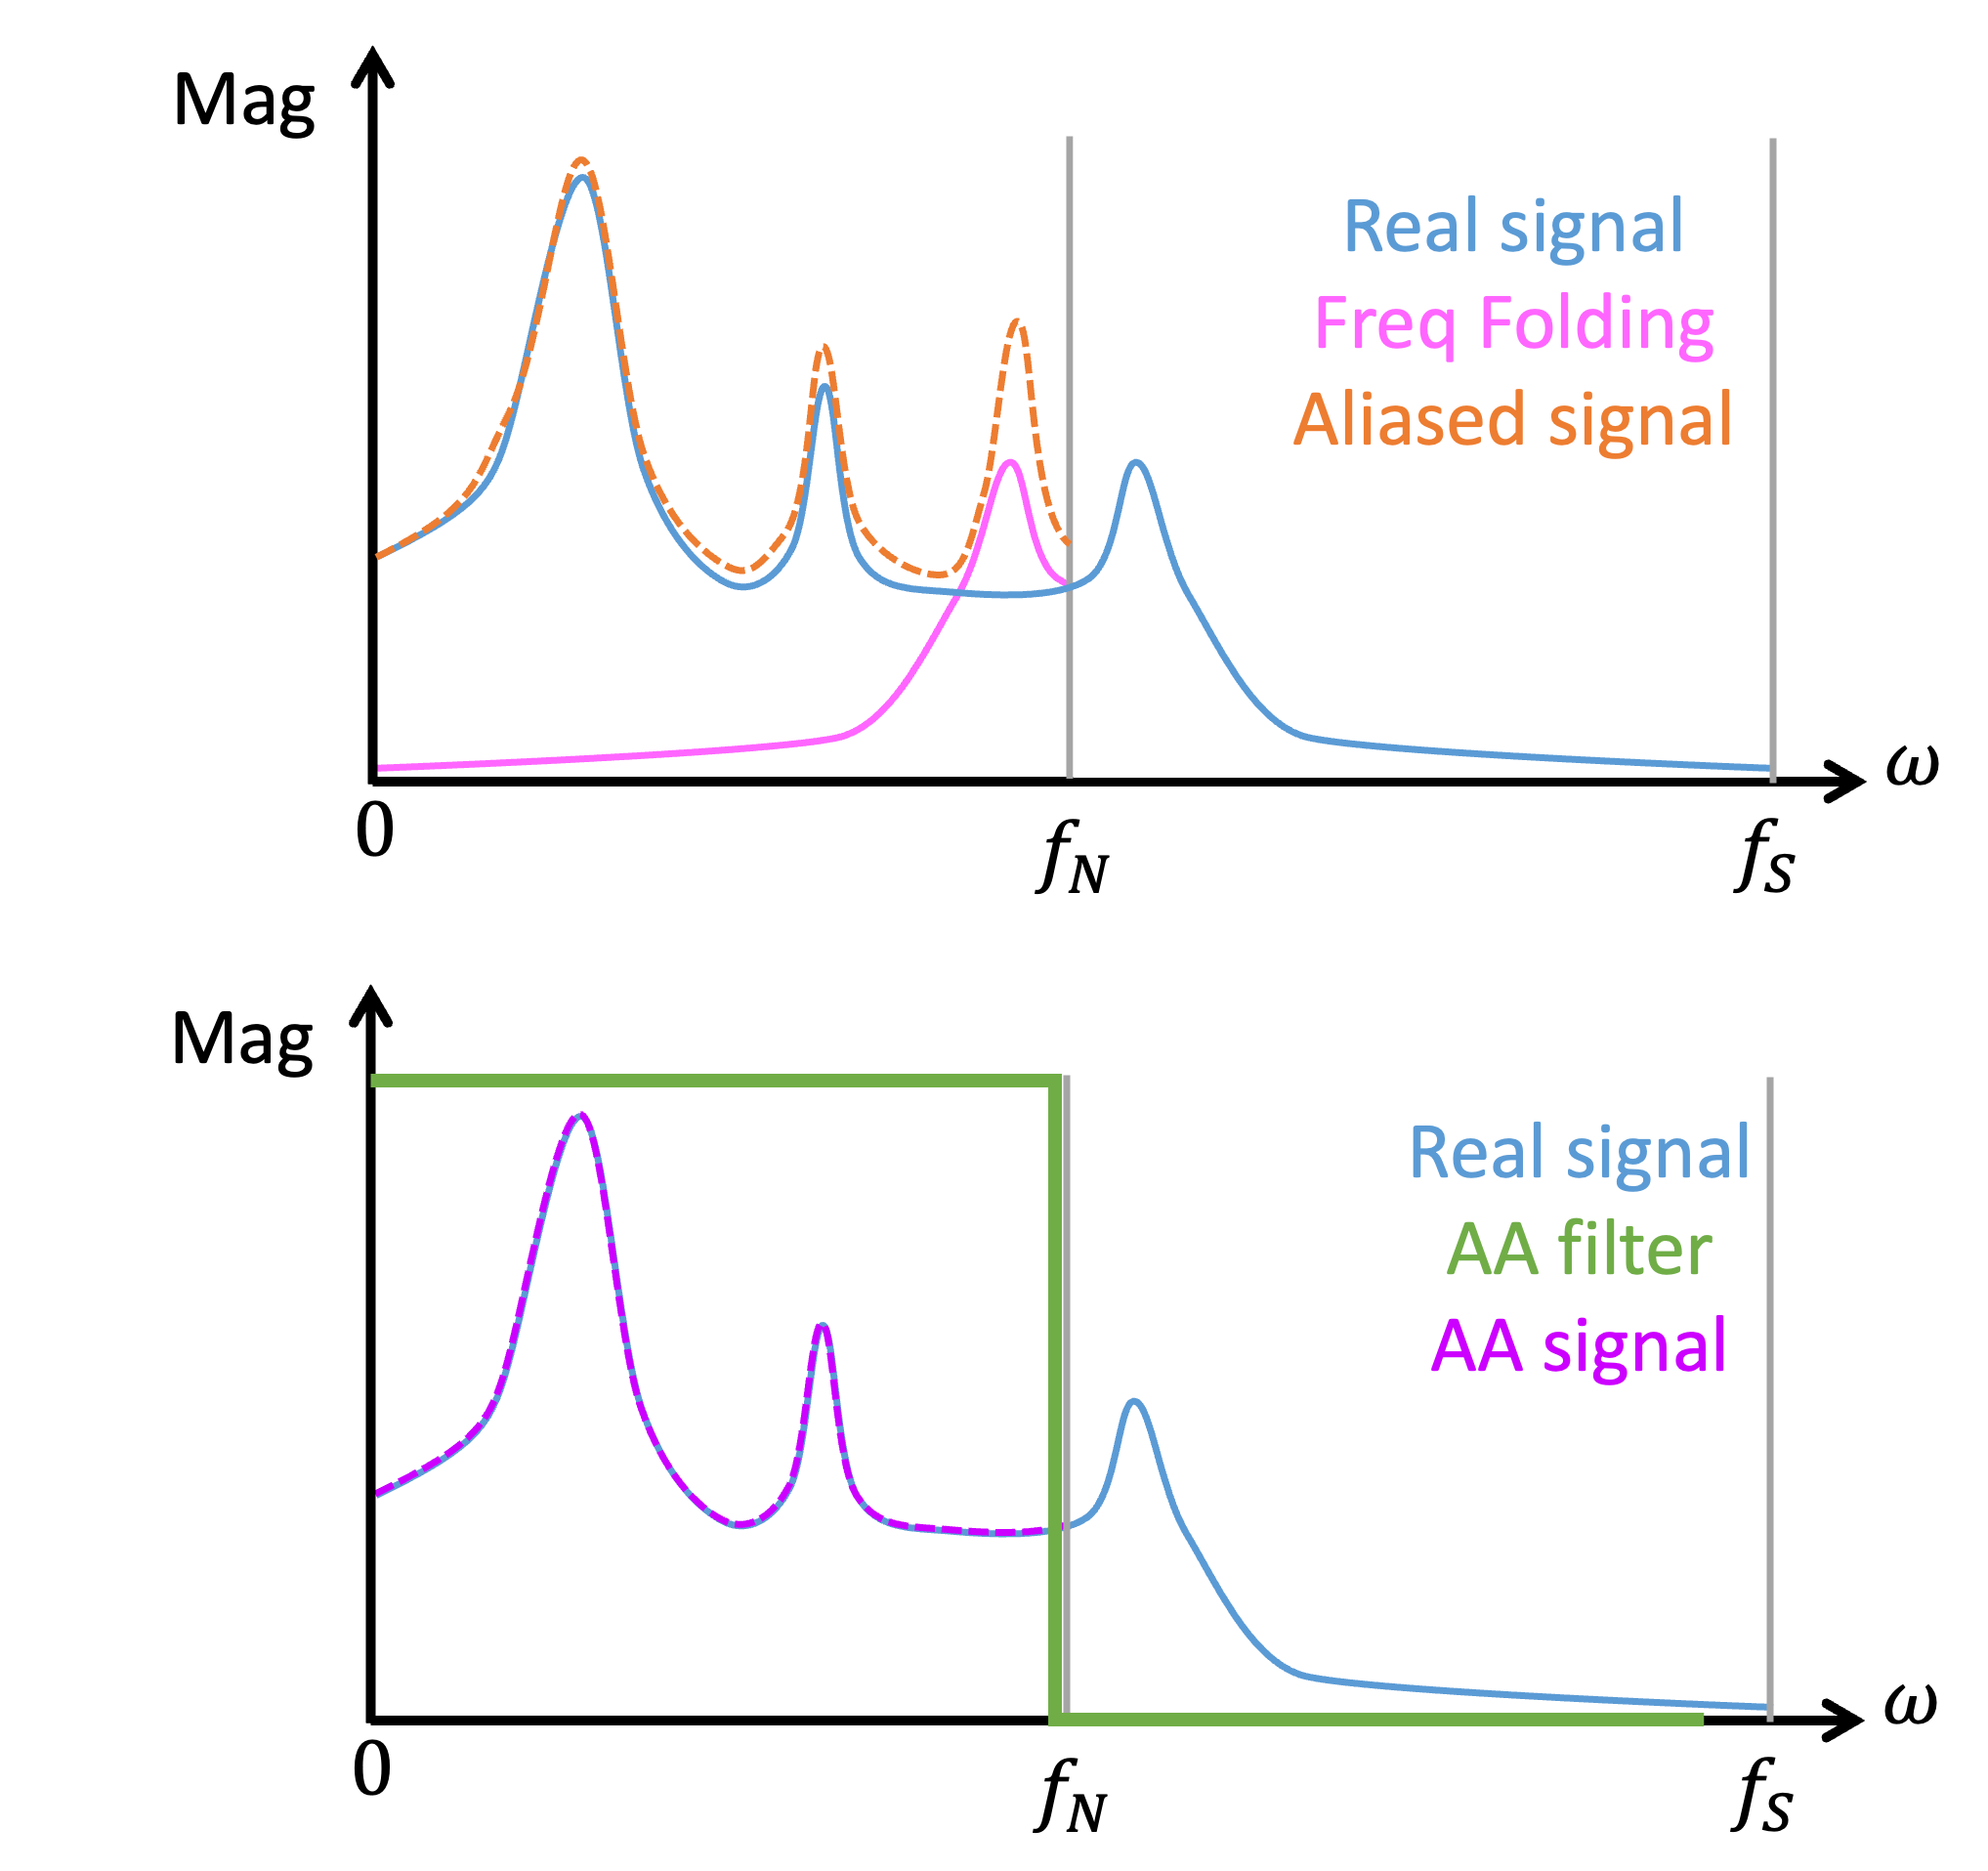
\includegraphics[width=5in]{Figuras/AAexample.png}
\end{figure}

\begin{itemize}
    \item Filtro anti-aliasing (AA) de paso bajo (low-pass) es utilizado para eliminar el ``aliasing'' de la respuesta en frecuencia.
    \item Filtro AA tiene que ser aplicado antes del muestreo en el tiempo.
\end{itemize}

\begin{figure}[H]
\centering
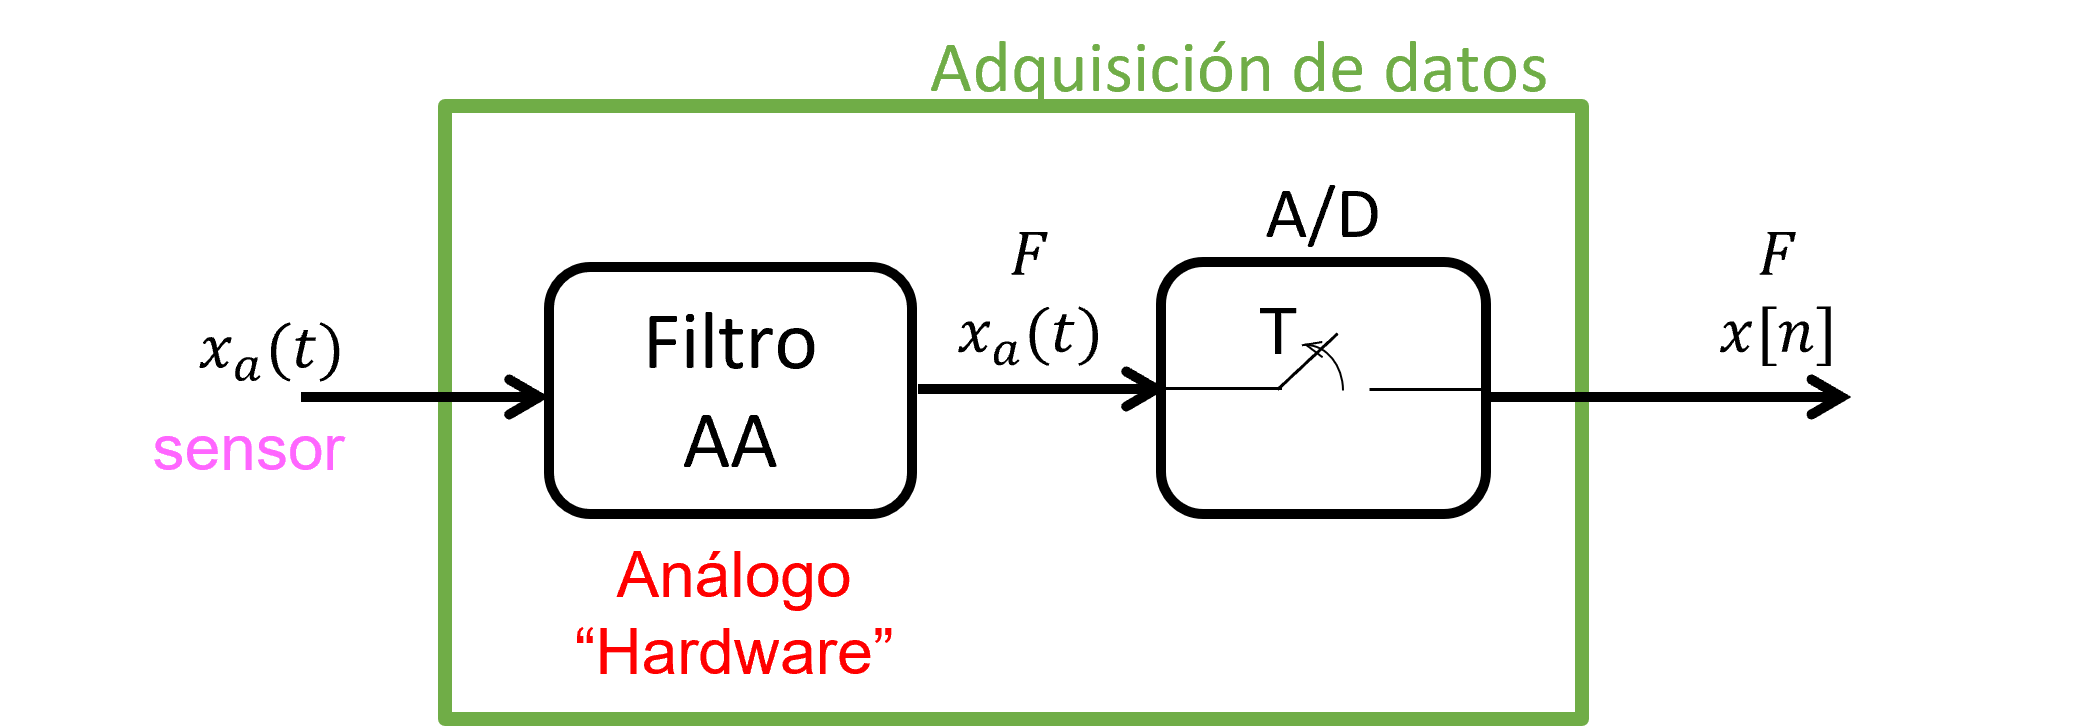
\includegraphics[scale=0.7]{Figuras/filtroAA2.png}
\end{figure}

\subsection{Spectral Leakage}
CTFT/DTFT/DFT asumen que la \underline{señal es periódica}, es decir, que la señal se repite luego de un periodo $T_1$ indefinidamente.
$$ x(t) = x(t+nT_1) $$
Si la señal no es periódica, ocurren saltos abruptos.
\begin{figure}[H]
\centering
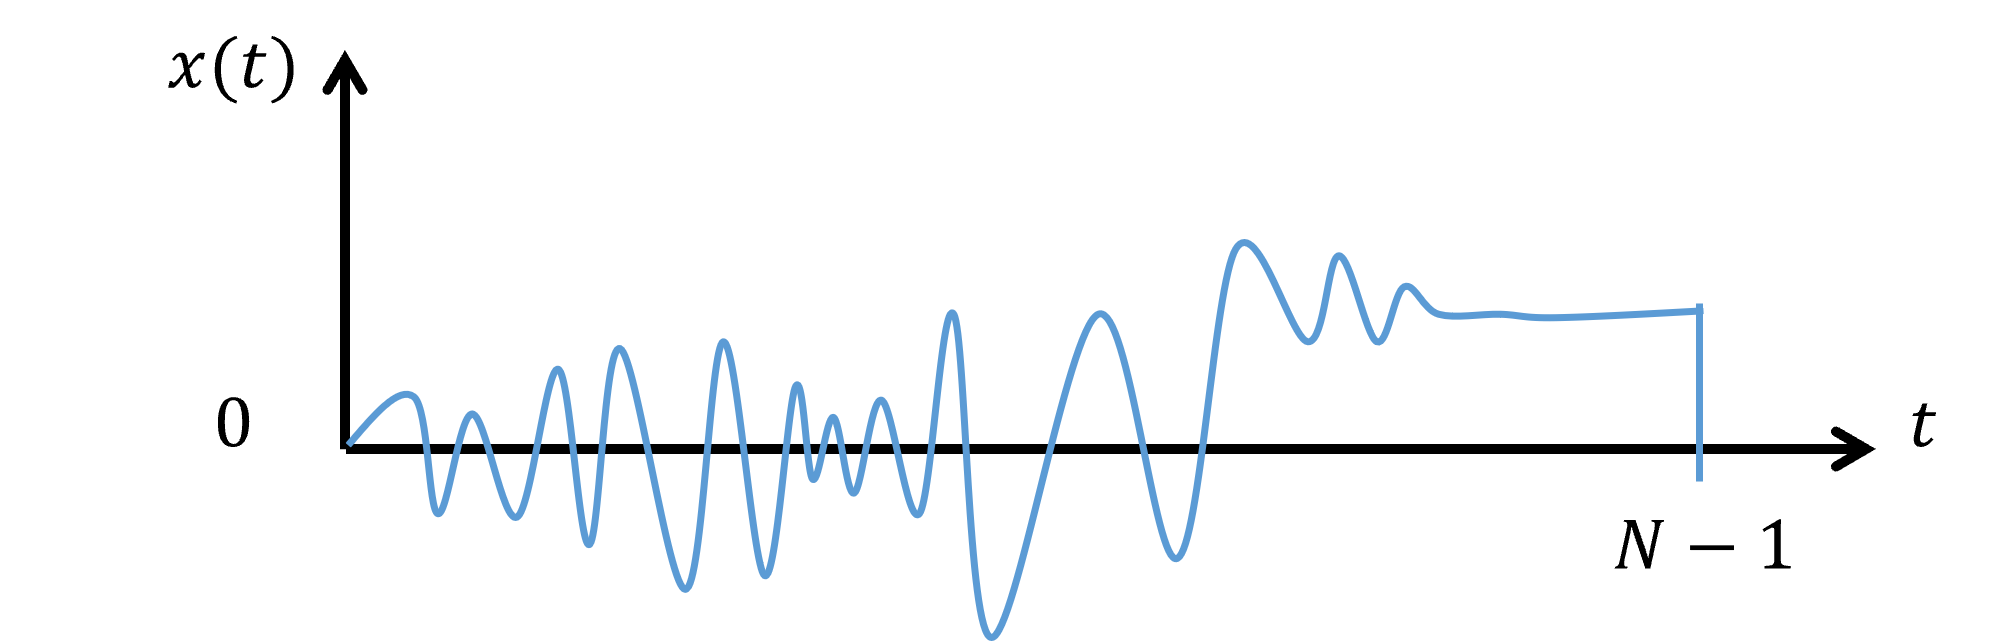
\includegraphics[scale=0.7]{Figuras/FT.png}
\end{figure}

\begin{figure}[H]
\centering
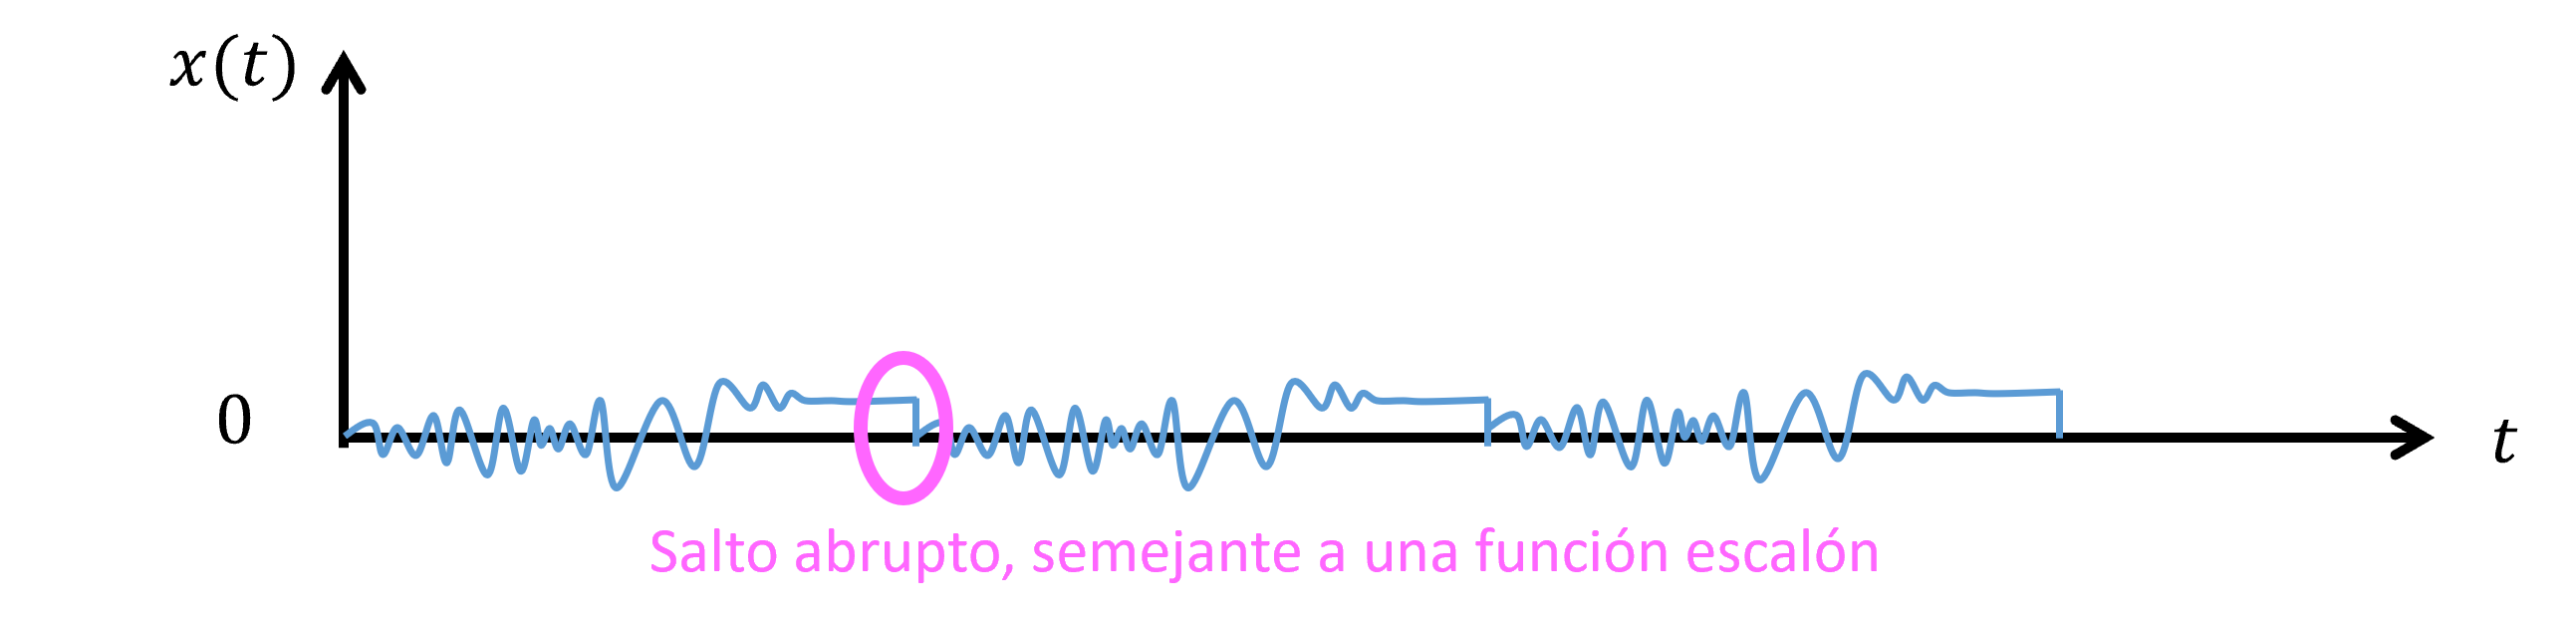
\includegraphics[scale=0.6]{Figuras/DFT.png}
\end{figure}

Este salto abrupto es semejante a una función escalón. Recordar que una función escalón se puede escribir como una Serie de Fourier que es una suma de armónicas con distinta frecuencia. Por lo tanto, al calcular $X[m]$ (DFT de $x[n]$) surge el fenómeno de ``spectral leakage'', donde se agregan armónicas artificiales producto del escalón generado.\\
\par \underline{Ejemplo}:

\begin{figure}[H]
    \centering
    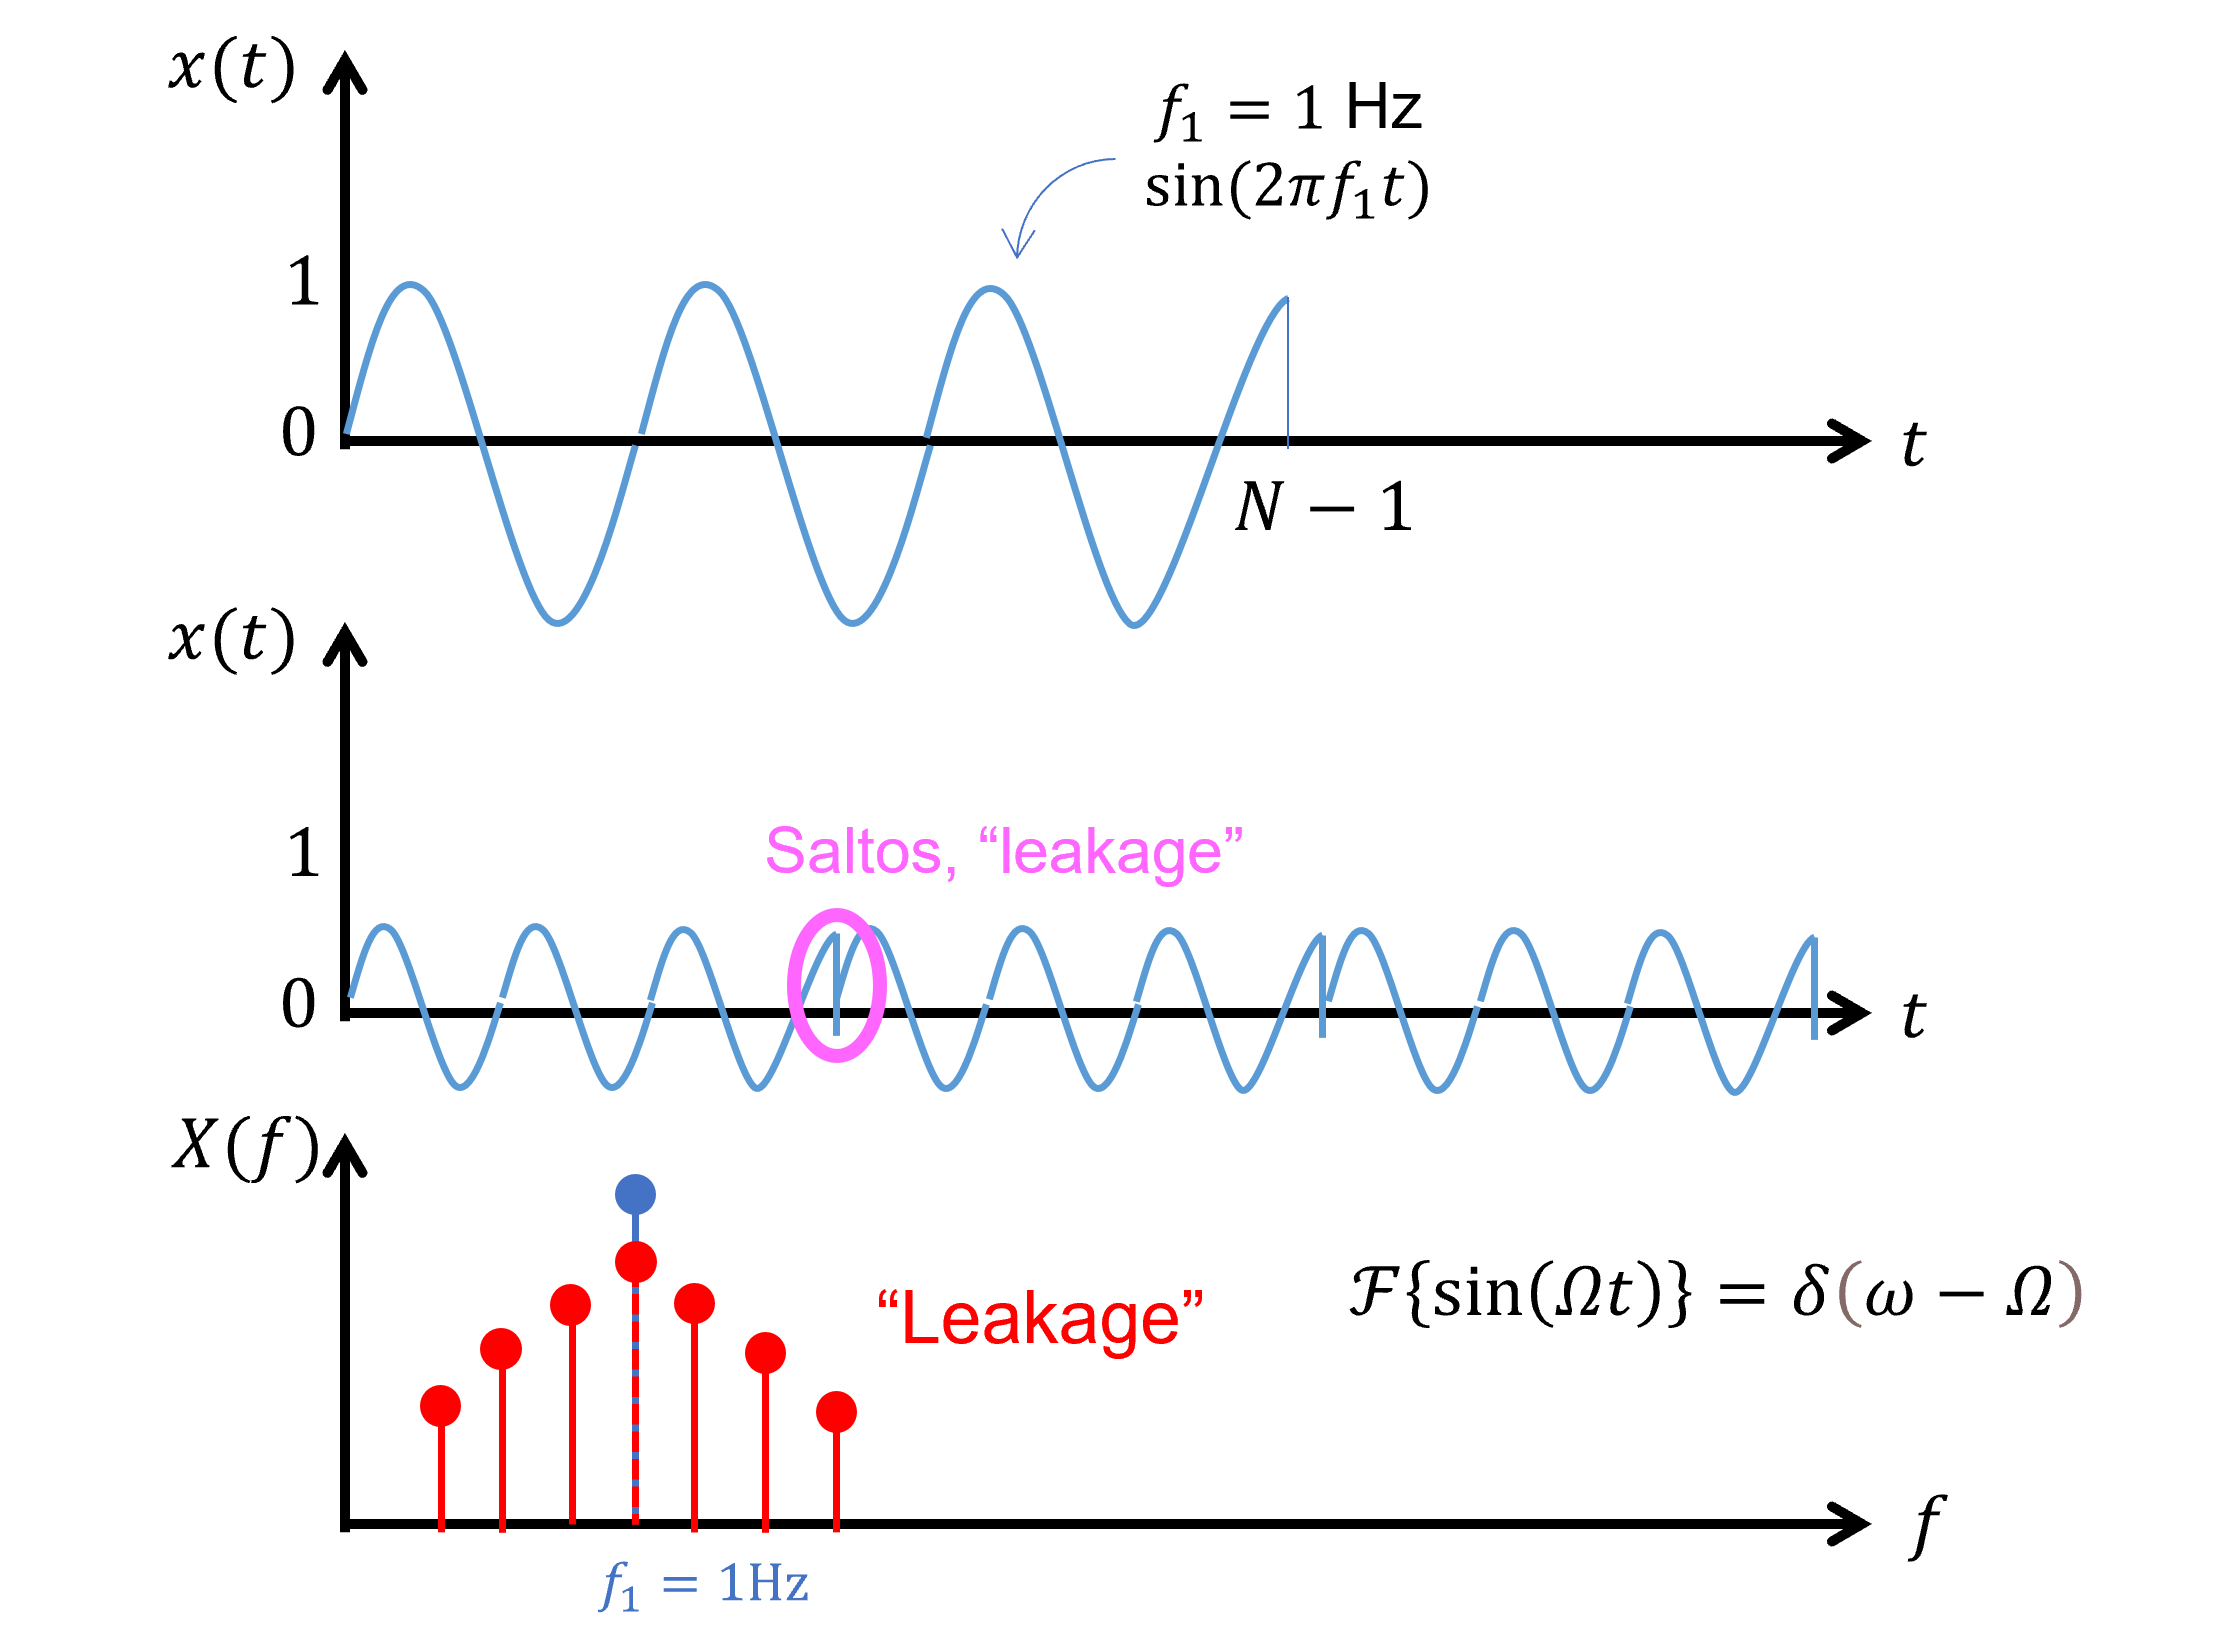
\includegraphics[width=5in]{Figuras/ejemplo_leakage.png}
\end{figure}

\par \underline{Solución}: ``Windowing'' $\Longrightarrow$ aplicar ventanas.\\

\begin{figure}[H]
    \centering
    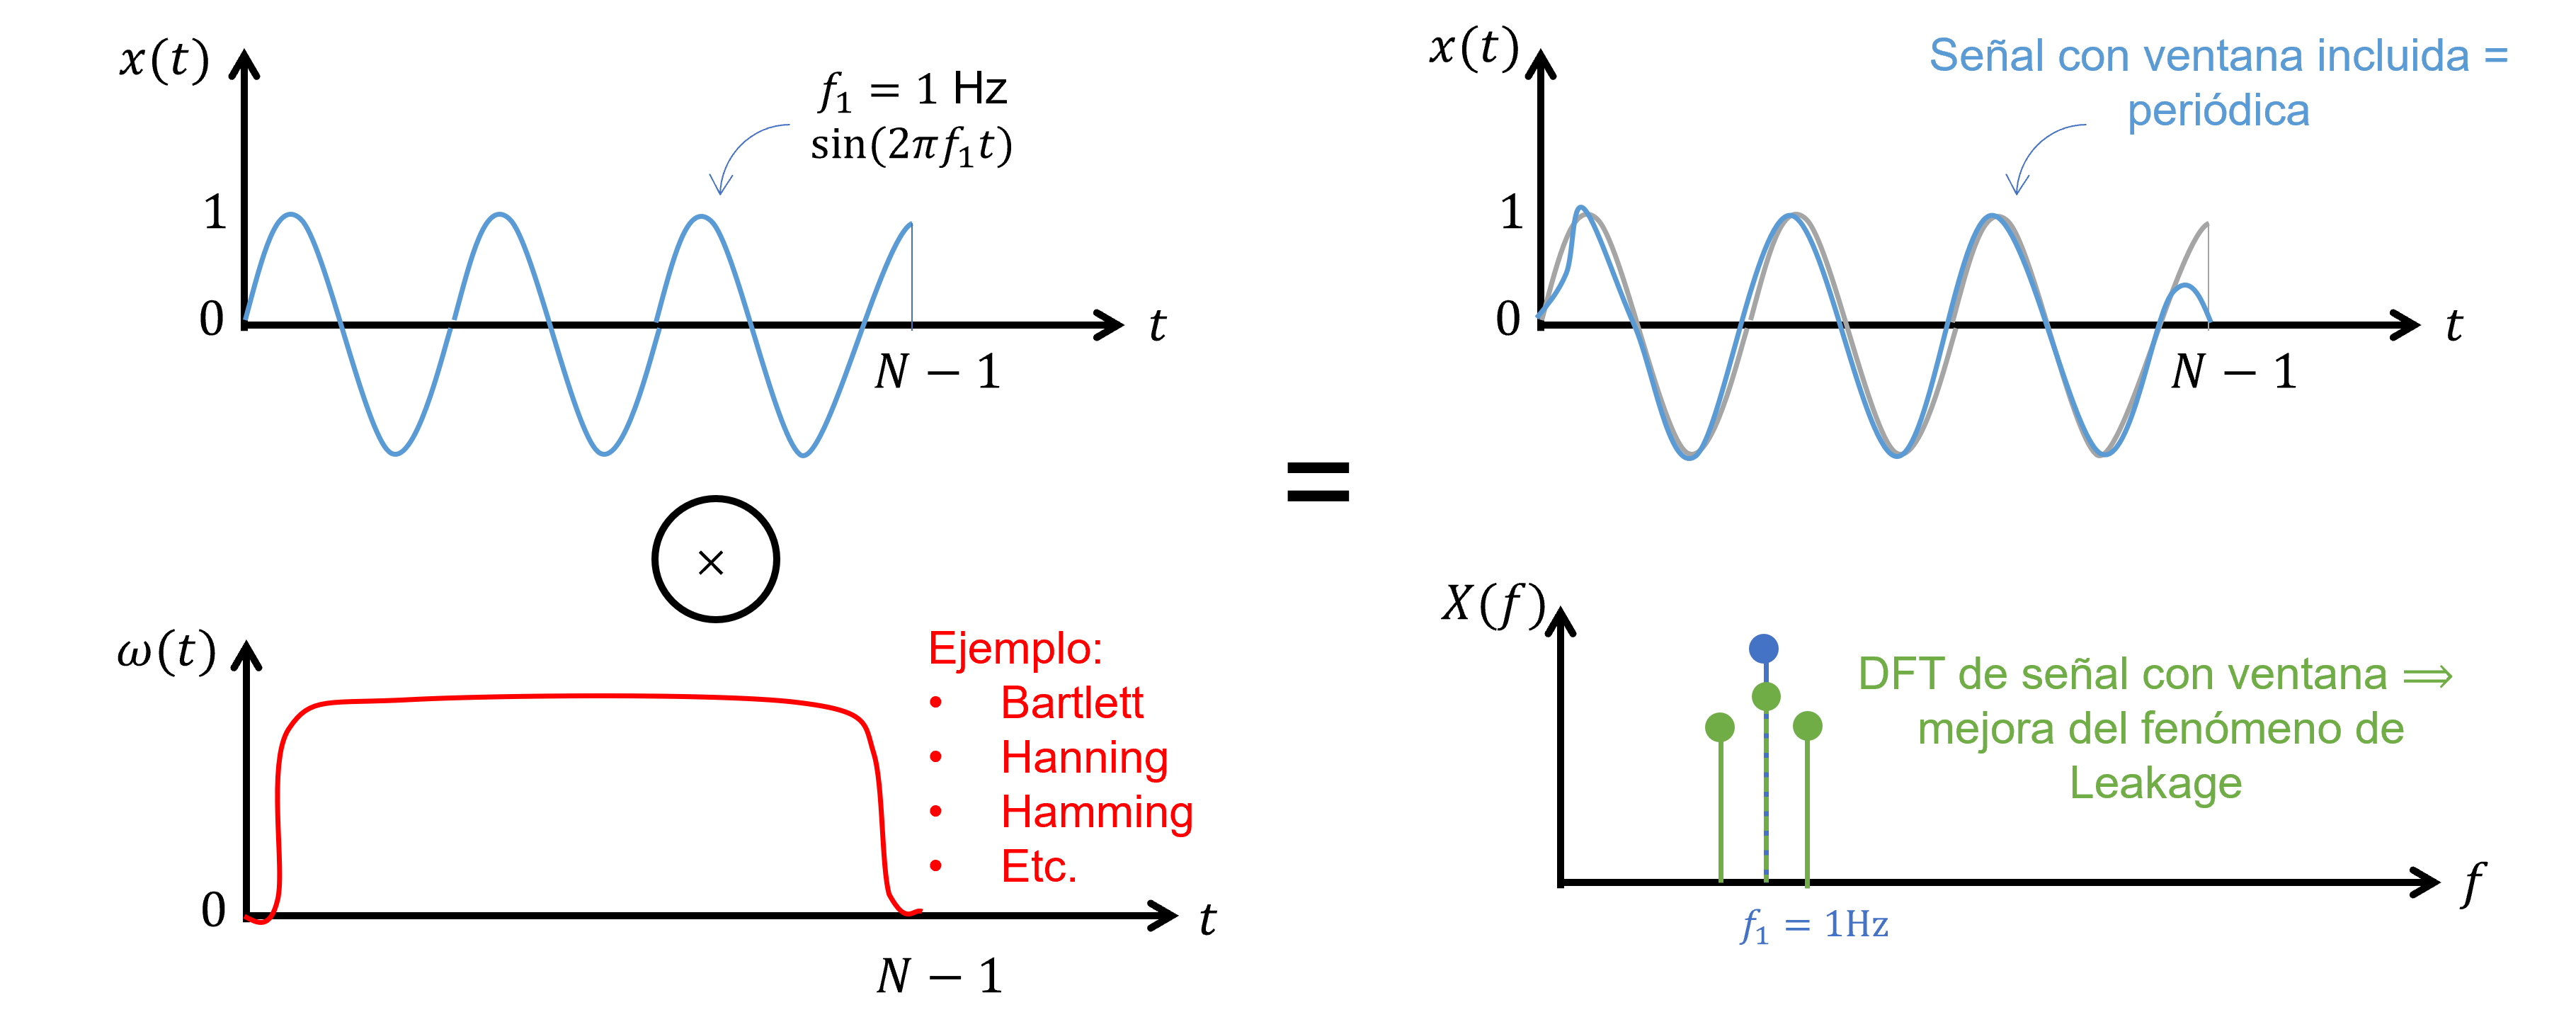
\includegraphics[width=\textwidth]{Figuras/solucion_leakage.png}
\end{figure}

También ocurre cuando la señal está contaminada con ruido. \\

Para resolver el \emph{spectral leakage} se pueden utilizar \emph{Periodogramas}.

\section{PSD de señal digital}

Referencia: \textcite[Cap. 8]{Hayes1996}.\\

En el caso de que $x(t)$ sea un p.e. w.s.s., su PSD se puede calcular de la siguiente forma:

\begin{align*}
    S_{X}(\Omega) &= \mathcal{F}\{R_{X}(\tau)\} \quad \text{(Caso contínuo, CTFT)} %\\
    %&= \mathbb{E}\{X(\omega)X^\ast(\omega)\} \quad \text{(Caso contínuo)} }
\end{align*}

En cambio, si $x[k]$ un p.e. w.s.s., señal digital con un intervalo de muestreo $T_s$. Podemos estimar $S_{X}(\omega)$ (continua) utilizando estimadores de valor medio y la definición de DTFT.

\begin{align*}
    \hat{S}_{X}(\omega) = \sum_{k=-\infty}^{+\infty}\hat{r}_x[k]e^{-j\omega k}
\end{align*}

donde el estimador de autocorrelación $\hat{r}_{X}[k]$, $n$ es el índice temporal, y $k$ es el índice para el retraso.

\begin{align*}
    \hat{r}_{X}[k] = \frac{1}{N} \sum_{n=0}^{N-1} x[n] x^*[n+k], \qquad k \in\{0,1,2,\ldots,N-1\}    
\end{align*}

\par Alcance para la estimación del PSD:

\begin{enumerate}
    \item Calcular DFT, y utilizar una forma de calcular el promedio de manera insesgada.
    \item Distintas realizaciones de $x(t)$ (de $x[k]$) nos entegan disintas estimaciones del PSD. \\ Cada estimación del PSD es una realización de un proceso estocástico.
\end{enumerate}

\begin{figure}[H]
    \centering
    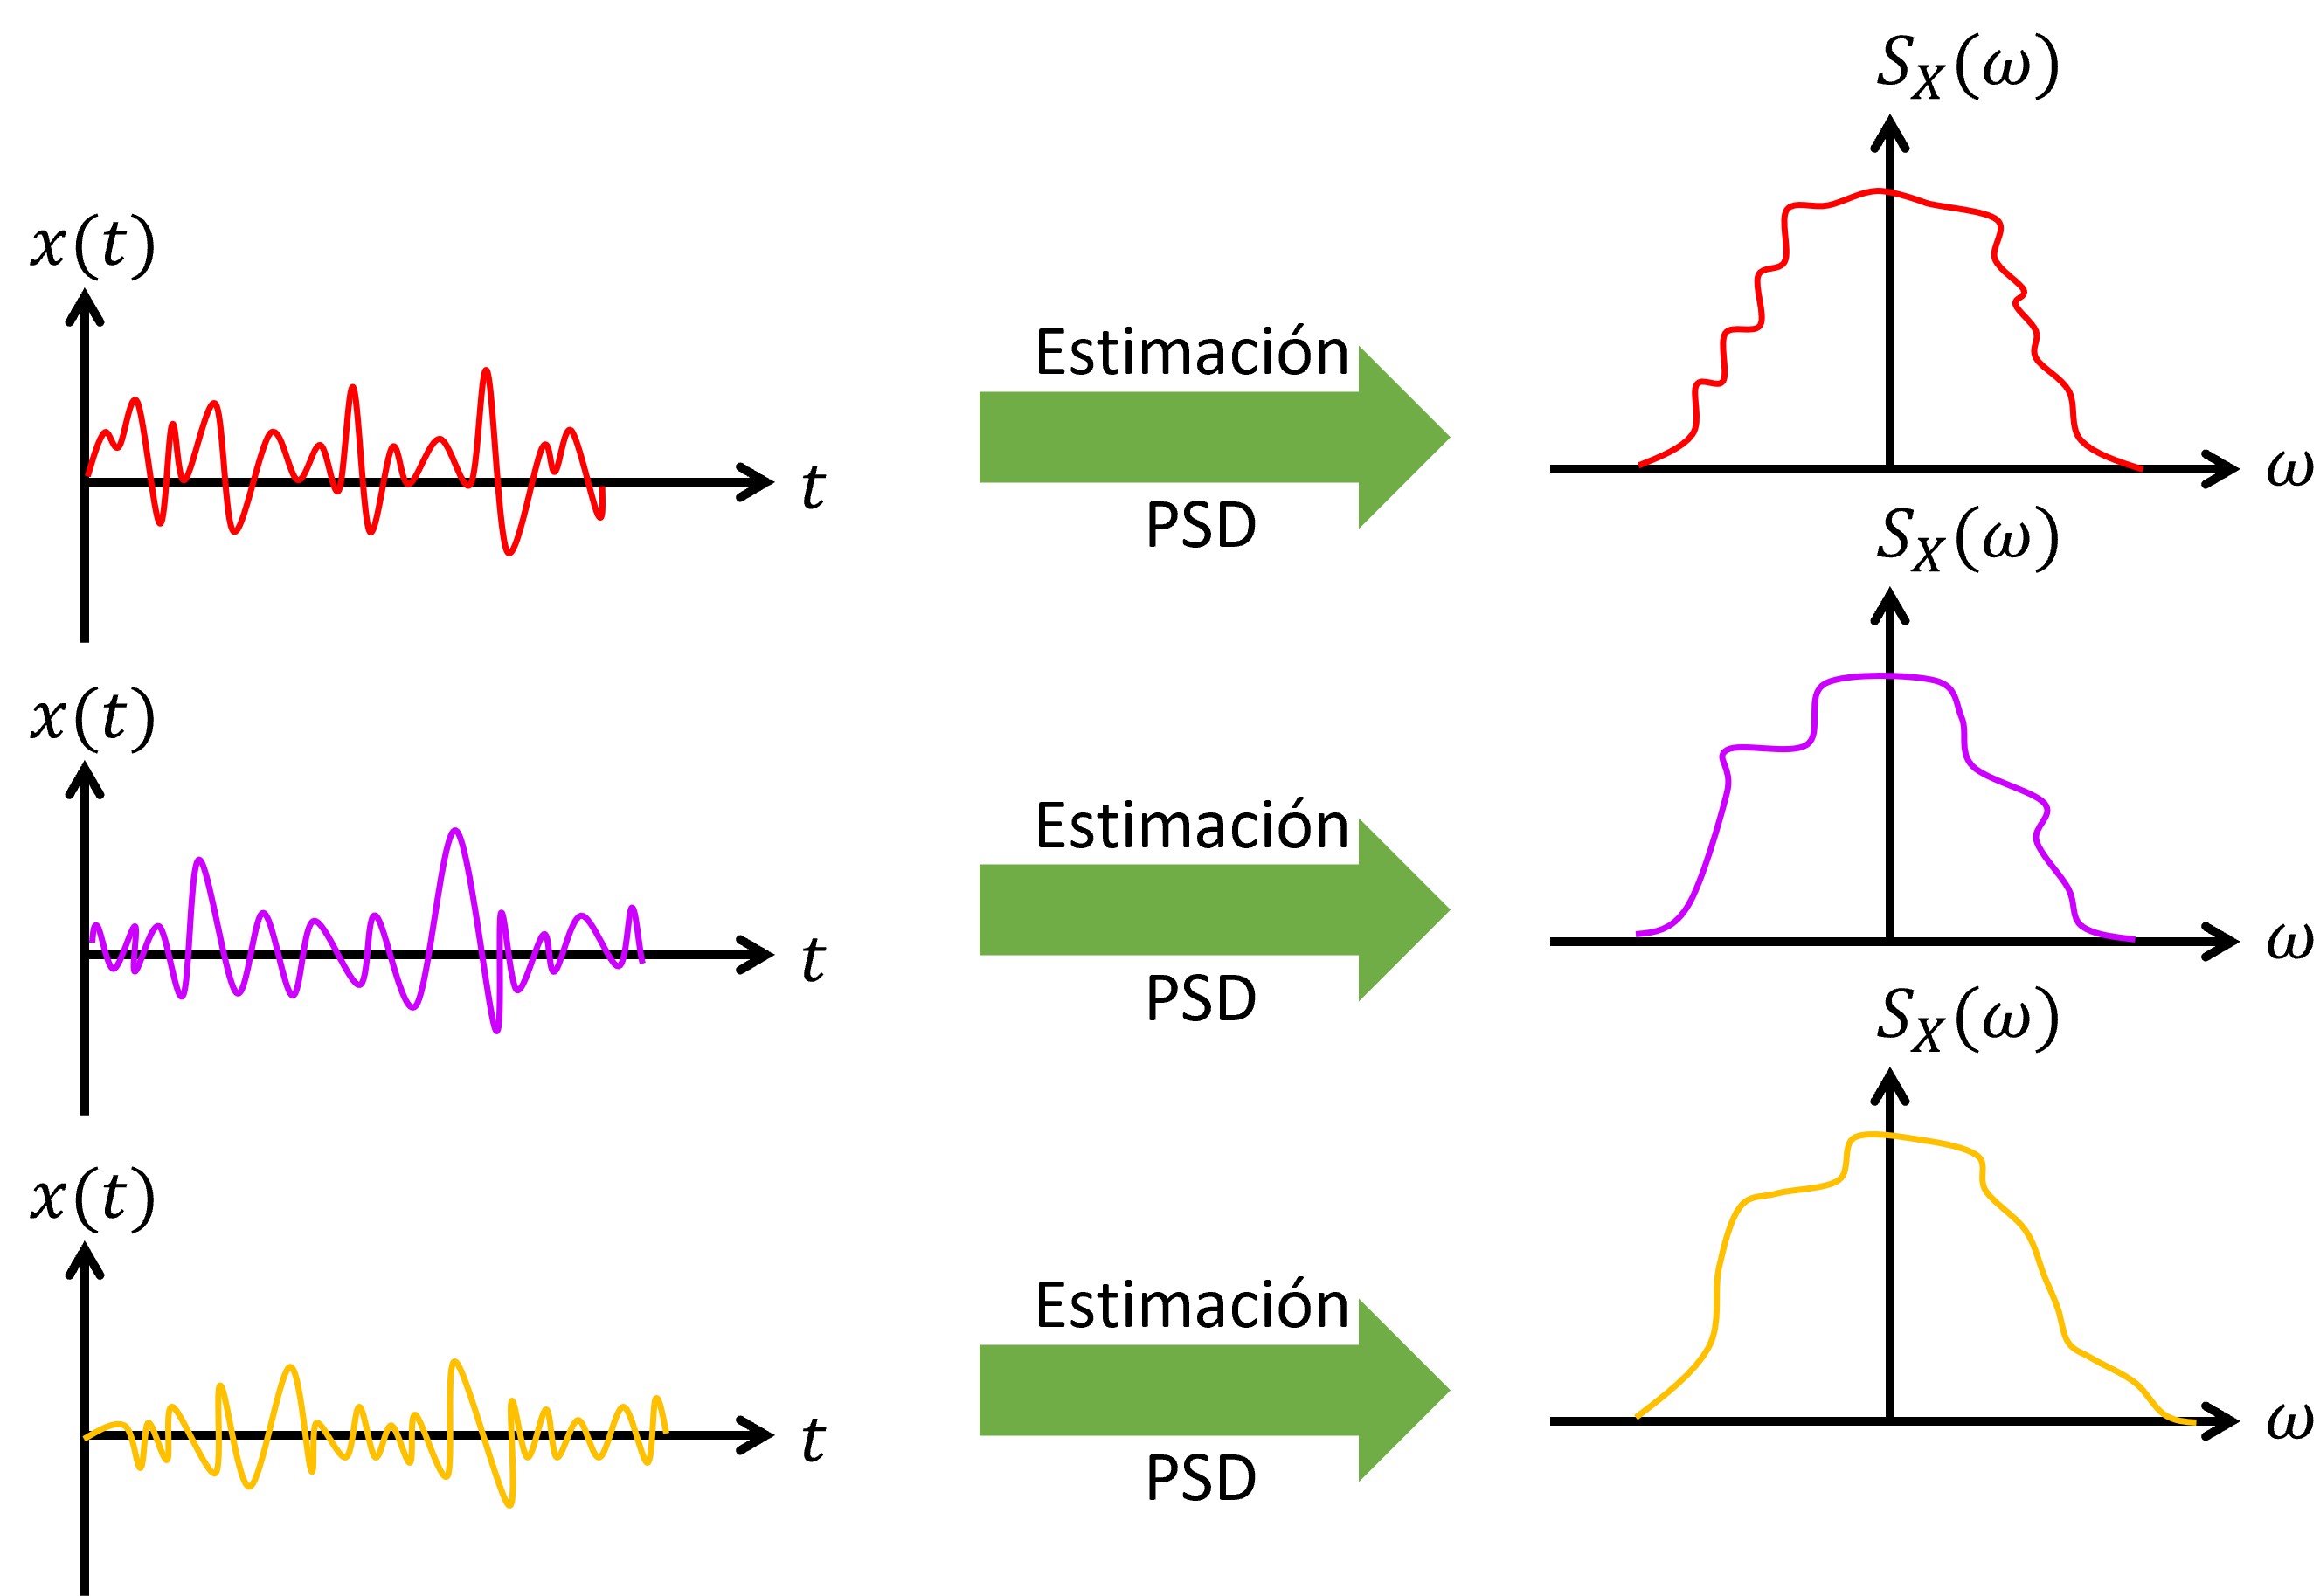
\includegraphics[scale=0.6]{Figuras/PSD_realizaciones.png}
\end{figure}

\par Estrategia para caracterizar el PSD:
\begin{enumerate}
    \item Queremos que la media del PSD se acerque al valor real del PSD.
    \item Queremos que la varianza del PSD sea pequeña.
\end{enumerate}

\underline{Ejemplo}: Considere el siguiente p.e.:
\begin{align*}
    x[n]=A+w[n]
\end{align*}

donde $A$ es una constante; $w[n] = w(nT_s)$ es ruido blanco, $\mu_W(t) = 0$ y $\sigma_W^2(t) = \sigma^2$. Entonces, $\mu_X(t) = A$ y $\sigma_X^2(t) =  \sigma^2$.\\

\par Dada una realización finita $\{x[0],x[1]...,x[N-1]\}$. Un estimador razonable para la media $A$ es la ``media muestral de A'' (promedio).

\begin{align*}
    \hat{A} = \frac{1}{N} \sum_{n=0}^{N-1}x[n]
\end{align*}

\par Entonces, queremos dos cosas:

\begin{enumerate}
    \item Que $\hat{A}$ sea insesgado, es decir, que converja al valor correcto de $A$: 
    
    $$\mathbb{E}\{\hat{A}\}=A$$
    
    Si $\hat{A}$ es sesgado. Que al menos cumpla con ser un estimador asintóticamente insesgado:
    
    $$\lim_{N\to\infty} \mathbb{E}\{\hat{A}\}=A$$
    
    \item La varianza de $\hat{A}$ sea pequeña
    
    $$\text{var}\{\hat{A}\} = \frac{\sigma^2}{N}$$ 

    En este sentido, la dispersión de $\hat{A}$ disminuye en la medida que $N$ aumenta:

    $$\lim_{N\to\infty} \text{var}\{\hat{A}\} = 0$$
    
    % \underline{Nota}: Quizás, aumentando N se disminuye la dispersión de $\hat{A}$
\end{enumerate}

\underline{Objetivos}: Estimar $\hat{S}_X(\omega)$ tal que:
$$\mathbb{E}\{\hat{S}_X(\omega)\}=S_X(\omega) $$ y 
$$\text{var}\{\hat{S}_X(\omega)\}=\text{pequeño} $$ 

\subsection{Periodograma}

\underline{Definición}: 

Usando DTFT:

\begin{align*}
    \hat{S}_{PER}(\omega) &= \frac{1}{N} \left| \sum_{n=0}^{N-1} x[n] e^{-j \omega n} \right|^2
    \\
    & = \frac{1}{N} |X(\omega)|^2\\
    & = \frac{1}{N} X(\omega) X^*(\omega)
\end{align*}

Usando DFT:

\begin{align*}
    \hat{S}_{PER}[k] &= \frac{1}{N} \left| \sum_{n=0}^{N-1} x[n] e^{-j 2 \pi n k /N} \right|^2 \\
    & = \frac{1}{N} \left| X[k] \right|^2\\
    & = \frac{1}{N} X[k] X^*[k]
\end{align*}

\underline{Nota}: 
\begin{itemize}
    % \item Considera el cálculo del DFT en vez de TF contínua
    %\item Considera un estimador neutral para el cálculo de la $\mathbb{E}\{\cdot \}$
    \item $\hat{S}_{PER}[k]$ es sesgado, pero es asintóticamente insesgado

    \begin{align*}
        \lim_{N\to\infty}\mathbb{E}\{\hat{S}_{PER}[k]\}=S_X[k]
    \end{align*}

    \item Varianza de $\hat{S}_{PER}[k]$ no tiende a cero para $N\to \infty$ $\Longrightarrow$ Problema

    \begin{align*}
        \text{var}\{\hat{S}_X(\omega)\}=\sigma^4  
    \end{align*}
    
    donde $\sigma^2=\frac{S_0 \omega_c}{\pi}$ si $x[n]$ es un ruido blanco.\\
    
\end{itemize}

Principales problemas del periodograma:

\begin{enumerate}
    \item Estimación sesgada
    \item Varianza no decrece con aumento $N$
    \item Fluctuaciones rápidas
    \begin{figure}[H]
    \centering
    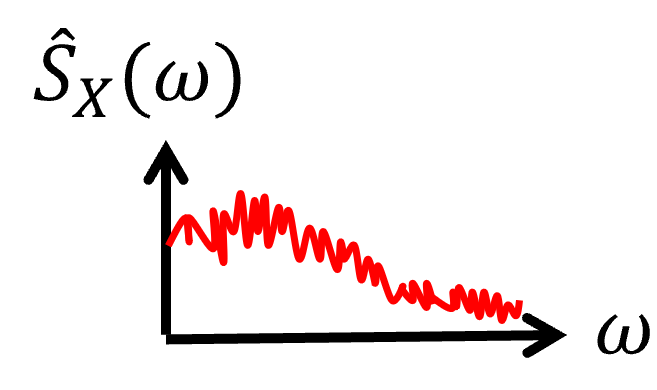
\includegraphics[scale=0.7]{Figuras/fluct.png}
    \end{figure}
\end{enumerate}

\subsection{Periodograma Modificado}

Métodos que modifican el periodograma clásico, para resolver los problemas estacionarios:

\begin{itemize}
    \item \underline{Periodograma modificada}: uso de ventanas, que reduce el efecto del sesgo, pero sacrificando resolución.
    
    $$\hat{S}_{MP}(\omega)=\frac{1}{N U} \left| \sum_{n=0}^{N-1} x[n]w[n]e^{-j\omega n} \right| ^2 $$
    
    donde $w[n]$: ventana en el dominio del tiempo y $U$ es un factor de escala.
    
    $$U=\frac{1}{N}\sum_{n=0}^{N-1}  w[n]^2$$

    Nota: $U=1$ si la ventana es rectangular.

    Desempeño:

    \begin{itemize}
        \item Reduce sesgo, pero sigue siendo una estimación sesgada.
        \item Es asintóticamente insesgada.
        \item La varianza es bastante cercana a la del periodograma.
    \end{itemize}
    
    \item \underline{Método de Bartlett}: promedio de periodogramas). Dividir la señal en $K$ segmentos de $L$ muestras, tal que $N = KL$.
    
    \begin{figure}[H]
        \centering
        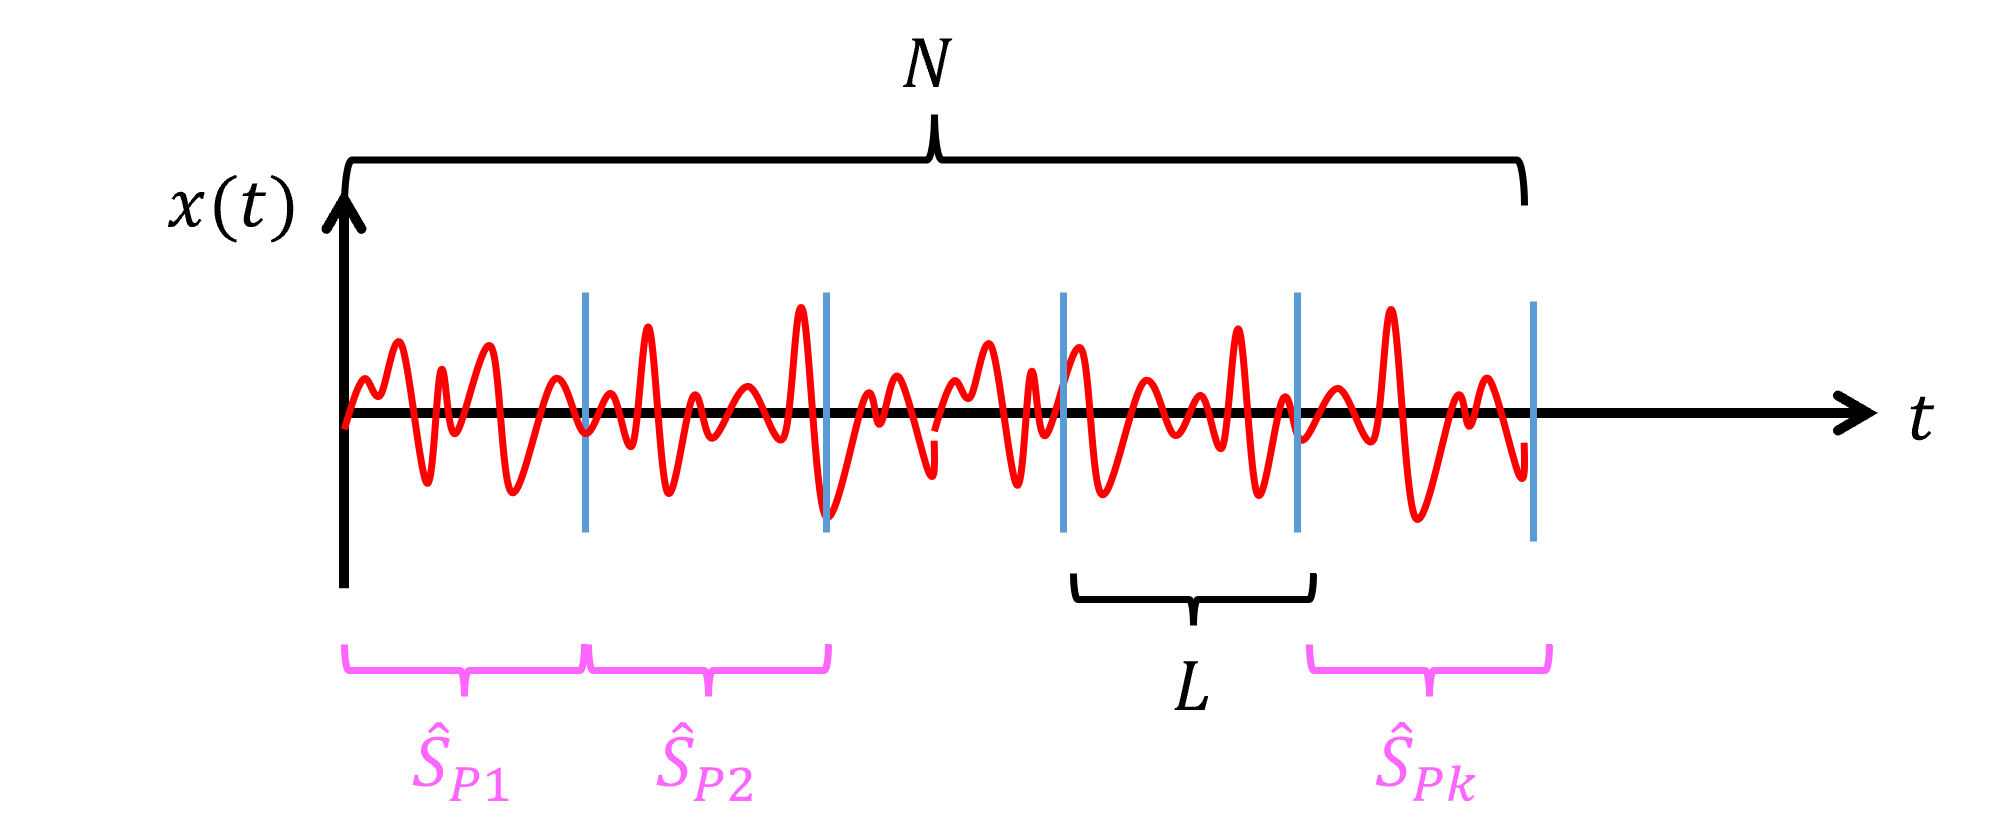
\includegraphics[scale=0.7]{Figuras/ventana1.png}
    \end{figure}

    Definición de bloque:

    $$
    x_i[n] = x[n + iL], \qquad
    \begin{cases}
        n &= \{0,1,\ldots,L-1\} \\
        i &= \{0,1,\ldots,K-1\}
    \end{cases}
    $$

    Entonces, la estimación del PSD es:
    
    $$\hat{S}_B(\omega)=\frac{1}{K}\sum_{i=0}^{K-1} \left\{\frac{1}{L} \left|\sum_{n=0}^{L-1}x_i[n]e^{-j\omega n} \right|^2 \right\} $$
    
    donde $i$ esta asociado al bloque $i$ de tamaño $L$.

    La varianza de la estimación del PSD es inversamente proporcional a la cantidad de bloques $K$:
    
    $$\text{var}\{\hat{S}_B(\omega)\} \propto \frac{1}{K}$$
    
    Es decir, que mientras más bloques se escogan (mayor $K$) más nos acercamos al objetivo de que la varianza sea $0$. \\
    
    El problema es que como $N = KL$, si se definen más bloques (aumentar $K$), significa que los bloques son más cortos ($L$ disminuye) y bloques cortos implican una resolución en frecuencia baja, es decir, $\Delta \omega$ es grande.
    
   % $$X[k] = \sum_{n=0}^{L-1}x[n]e^{-j2\pi nk/L} \quad \text{(DFT)}$$
    
    $\Longrightarrow$ ``Trade-off'': Varianza vs resolución.
    
    \item \underline{Método de Welch}: promedio de periodogramas con ventanas traslapadas.
    
    \begin{figure}[H]
        \centering
        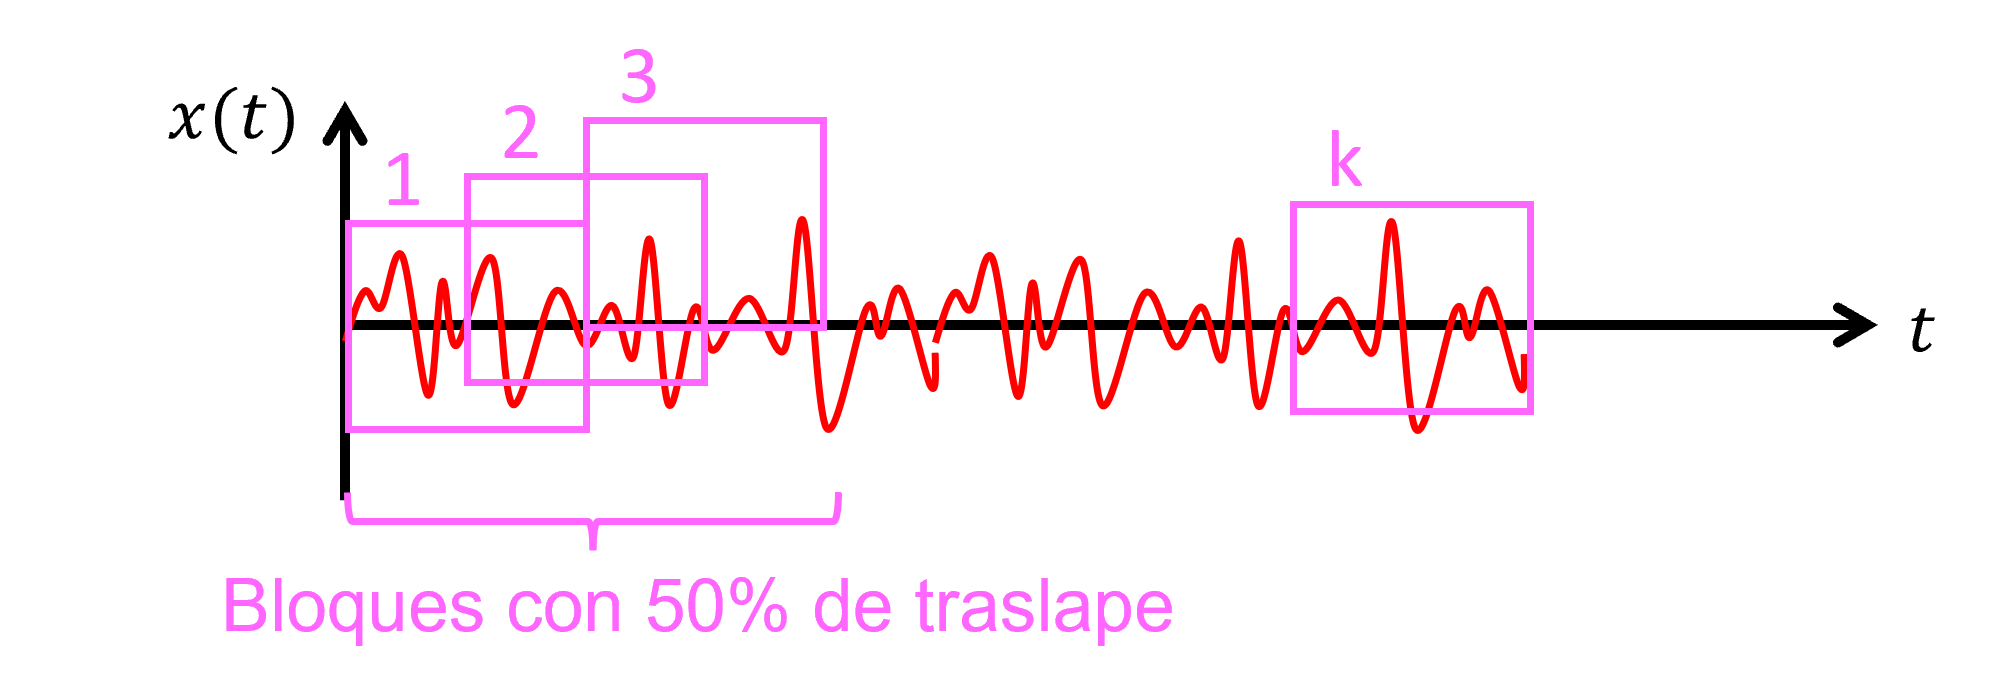
\includegraphics[scale=0.7]{Figuras/ventana2.png}
    \end{figure}

    Definición de bloque:

    $$
    x_i[n] = x[n + iD], \qquad
    \begin{cases}
        n &= \{0,1,\ldots,L-1\} \\
        i &= \{0,1,\ldots,K-1\}
    \end{cases}
    $$

    donde la cantidad de puntos de traslape es $L-D$:

    $$
    \begin{cases}
        D = L, & \text{sin traslape} \\
        D = L/2, & \text{50\% traslape (más común)}\\
        D = 3L/4, & \text{25\% traslape}
    \end{cases}
    $$
    
    $$\hat{S}_W (\omega) =\frac{1}{KLU}\sum_{i=0}^{K-1}\left| \sum_{n=0}^{L-1} x_i[n]w[n]e^{-j\omega n} \right|^2$$

    % La varianza de la estimación del PSD es inversamente proporcional a la cantidad de bloques $K$:
    
    % $$\text{var}\{\hat{S}_W (\omega)\} \approx \frac{9}{16}\frac{L}{N} S_X(\omega)^2 $$

    Comparado con método de Bartlett (sin traslape), para el mismo valor de $N$ y $L$, el método de Welch arroja casi un 50\% de reducción en varianza:

      $$\text{var}\{\hat{S}_W (\omega)\} \approx \frac{9}{16} \text{var}\{\hat{S}_B (\omega)\} $$
    
    En \emph{MATLAB}, la función \texttt{cpsd()} y \texttt{pwelch()} utilizan el método de Welch.
    
    % \item \underline{Método de Blackman-Tukey}:

    % \emph{(En desarrollo)}

    % En \emph{MATLAB}, la función \texttt{spa()} utiliza el método de Blackman-Tukey. Link: \url{https://www.mathworks.com/help/ident/ref/spa.html}.
    
\end{itemize}

\part{Aplicaciones}

\chapter{Sistemas de Control Estructural}

% NOTA: Utilizar apuntes de Manuel Ruiz Sandoval como guía
% Papers: 
% - Symans et al. 2008 - Energy Dissipation Systems for Seismic Applications: Current Practice and Recent Developments
% - Housner et al, 1997 - Structural Control. Past, Present, and Future
% - Saaed et al, 2015 - A State-of-the-art review of structural control systems
% - 

%% Anotaciones - Ideas
% En sistemas de control estructural, en introducción, poner la formula general de un sistema con control Mxpp + Cxp + Kx = F_externas + F_control
% Explicar que F_control tiene varias formas de diseñarse
% En vez de explicar los dispositivos de control en secciones de control pasivo, activo, semi-activo e híbrido... poner una sección de tipos de control explicandolos brevemente.
% Luego, crear secciones de modelos de sistemas de control, explicar brevemente como se modelan y ecuaciones de TMD, Amortiguador viscoso, Disipador histerético, BRB, 
%

\section{Introducción}
% Some from Saaed et al 2015
Los sistemas de control estructural son dispositivos mecánicos que se incorporan a una estructura para poder mejorar su desempeño y serviciabilidad ante cargas dinámicas.

\begin{itemize}
    \item Reducir la \underline{respuesta}
    \item Reducir \underline{pérdidas por daños}
    \item Reducción de \underline{riesgos} (Ej. Probabilidad de colapso)
\end{itemize}

\vspace{1eX}

Se clasifican en los siguientes grupos:

\begin{description} 
    \item[Pasivos] Estos sistemas no requieren una fuente de energía externa para operar. Funcionan disipando o absorbiendo la energía que ingresa a la estructura basándose únicamente en sus propiedades físicas y en el propio movimiento de la estructura.
    \item[Activos] Estos sistemas requieren una fuente de poder externa significativa (electricidad, sistema hidráulico) para funcionar. Utilizan sensores que miden la respuesta de la estructura en tiempo real y un algoritmo de control que calcula una fuerza de corrección. Luego, los actuadores aplican activamente esa fuerza a la estructura para contrarrestar la vibración.
    \item[Semi-Activos] Estos sistemas representan un punto intermedio inteligente. Requieren una pequeña cantidad de energía (como la de una batería), pero esta energía no se usa para aplicar fuerzas directamente a la estructura (como en el control activo). En cambio, se utiliza para cambiar las propiedades mecánicas (rigidez o amortiguación) del dispositivo de control en tiempo real.
    \item[Híbridos] Como su nombre indica, estos sistemas combinan dos o más de los tipos anteriores para aprovechar sus ventajas.
\end{description}


En general, las estructuras con dispositivos de control tienen la siguiente EDM:

\begin{align*}
    {M}{\ddot{q}} + {C}{\dot{q}} + {K}{q} + {f}_{p} + f_{s} = {f}_a + {f}_e
\end{align*}

\noindent donde ${f}_{p}$ es la fuerza de dispositivos pasivos, ${f}_{sa}$ es la fuerza de dispositivos semi-activos, ${f}_a$ es la fuerza de dispositivos activos, y ${f}_e$ es la fuerza externa (p.ej., terremoto).

\section{Control pasivo}
Los sistemas de control pasivo no requieren de una fuente de energía externa. \\

Funcionan absorbiendo, aislando y disipando energía. \\

Su operación puede depender tanto de el desplazamiente, velocidad y aceleración relativa entre los nodos de conexión del dispositivo. Algunos de estos dispositivos requieren ser reemplazados luego de ser utilizados. \\

% La ecuación general para un sistema estructural con dispositivos de control pasivo es:

% \begin{align}
%     {M}{\ddot{q}} + {C}{\dot{q}} + {K}{q} + \textcolor{red}{{f}_p(q,\dot{q},\ddot{q})} = {f}_e
% \end{align}

\subsubsection{Amortiguadores viscosos}

\begin{equation}
    f_p(\dot{r}) = c_d |\dot{r}|^\alpha \text{sign}(\dot{r})
\end{equation}

\subsubsection{Amortiguadores metálicos}

Disipación de energía por histeresis. Por ejemplo, usando un modelo de Bouc-Wen:

\begin{align}
    f_P(r,\dot{r},t) = (1-\alpha) k r +  \alpha k z(t)
\end{align}

donde $z(t)$ es un estado interno que maneja la histeresis del dispositico, y que evoluciona a través de una ecuación diferencial nolineal:

\begin{align}
    \dot{z} = h(\dot{r},z)
\end{align}

\subsubsection{Amortiguadores de fricción}

\begin{align}
    f_P(\dot{r},t) = \mu(t) N(t) \text{sign}(\dot{r})
\end{align}

donde $\mu(t)$ es el coeficiente de fricción dinámico, $N(t)$ es la fuerza normal en la superficie de deslizamiento, y $\dot{r}$ es la velocidad relativa entre los terminales del amorgtiguador de roce.

% \subsubsection{Dispositivos Viscoelásticos}

% Comunmente son pistones que consisten en cilindros huecos rellenos de un material viscoelástico (fluido o sólido). En el caso de meteriales fluidos, la fuerza se genera cuando el fluido orificios y en el caso de materiales sólidos ocurre cuando estos se deforman. 

% Para modelar las fuerzas:
% \begin{align*}
%     P(t) &= C|\dot{u}(t)|^\alpha \text{sign}[\dot{u}(t)] \longrightarrow \text{VE Fluidos} \\
%     P(t) &= Ku(t) + C\dot{u}(t) \longrightarrow \text{VE Sólidos}
% \end{align*}
% La disipación de energía ocurre por la fricción generando calor.


\subsection{Amortiguadores de masa sintonizada}

\begin{align}
    f_P = m_{TMD} a_{TMD}
\end{align}

donde $a_{TMD}$ es la aceleración absoluta del TMD.

% \subsubsection{Otros}

% \begin{itemize}
%     \item Dispositivos de re-centrado
%     \item Amortiguadores de transformación de fase
%     \item Amortiguadores/disipadores de vibración dinámica:
%     \begin{itemize}
%         \item Amortiguadores de Masa Sintonizada (TMD)
%         \item Amortiguadores de Líquido Sintonizado (TLD)
%     \end{itemize}
% \end{itemize}


% \subsubsection{Dispositivos de Aislación Sísmica}
% % Saaed

% \begin{itemize}
%     \item Eficiente para vibraciones desde el suelo como sismos y tráfico, no para viento.
%     \item Alta flexibilidad lateral
%     \item Alta rigidez vertical
%     \item Inclusión de nuevo modo de vibrar con \emph{Desplazamientos relativos entre piso} pequeños.
%     \item Al incluir el nuevo modo de vibrar, se alejan los otros modos lejos del contenido de periodos de la excitación.
%     \item Funcionan para edificios bajos con periodos fundamentales cortos y no para edificios altos que tienen periodos fundamentales largos.
%     \item Se puede incluir en distintas ubicaciones de la estructura.
% \end{itemize}

% Los dispositivos de aislación sísmica basan su funcionamiento en la flexibilidad horizontal de un nivel pero una alta rigidez vertical. Debido a la flexibilidad horizontal, se introduce un nuevo modo de vibrar que contiene \emph{desplazamientos relativos entre pisos} pequeños. 

\section{Control activo}

Los dispositivos de control activo requieren de energía para contrarrestar la respuesta estructural. Funcionan adaptandose en función de la excitación y respuesta. Requieren del uso de sensores y actuadores. La ecuación general es la siguiente:

\begin{align}
    {M}{\ddot{q}} + {C}{\dot{q}} + {K}{q} = \textcolor{red}{{f}_a(q,\dot{q},\ddot{q},u)} + {f}_e
\end{align}

donde $f_a$ es la fuerza activa, que puede depender de estados del sistema, pero depende principalmente de una señal de control exógena $u(t)$.

\underline{Ventajas del control activo}:
\begin{itemize}
    \item Efectividad, no hay límites teoréticos para la eficiencia del controlador
    \item Adaptabilidad a la excitación
    \item Selectvidad, el controlador se puede diseñar para varios objetivos (seguridad y comfort)
    \item Aplicabilidad para un gran rango de frecuencias y excitaciones
\end{itemize}

\underline{Dispositivos}:
\begin{itemize}
    \item Amortiguador de masa activo (Active mass damper, AMD)
    \item Sistemas de tendones activos (Active tendon systems)
    \item (Active brace systems)
    \item (Pulse generation systems)
\end{itemize}

\section{Control semi-activo}

\begin{align}
    {M}{\ddot{q}} + {C}{\dot{q}} + {K}{q} + \textcolor{red}{{f}_s(q,\dot{q},\ddot{q},u)} = {f}_e
\end{align}

Ejemplo: Amortiguador viscoso de orificio variable. El coeficiente $c_d(u)$ es una función de una señal de control exógeno.

\begin{equation}
    f_{sa}(\dot{r},u) = c_d(u) |\dot{r}|^\alpha \text{sign}(\dot{r})
\end{equation}

\begin{itemize}
    \item TMD semi-activo (Semi-active TMDs)
    \item TLD semi-activo (Semi-active TLDs)
    \item Amortiguador de fricción semi-activo (Semi-active friction damper)
    \item (Semi-active vibration absorbers)
    \item Controlador de rigidez semi-activo
    \item Amortiguadores Electroreologicos (Electrorheological damper, ER)
    \item Amortiguador Magnetoreologico (MR)
    \item Amortiguador viscoelástico semi-activo
\end{itemize}

\section{Control híbrido}

\begin{itemize}
    \item Amortiguador de masa hibrido (Hybrid mass damper, HMD)
    \item Aislación basal híbrida: aislación basal + control activo o semi-activo
\end{itemize}


\chapter{Teoría de Control Clásico}

\section{Open-loop vs closed-loop control}
\subsection{Open-loop (feedforward)}
\begin{figure}[H]
\centering
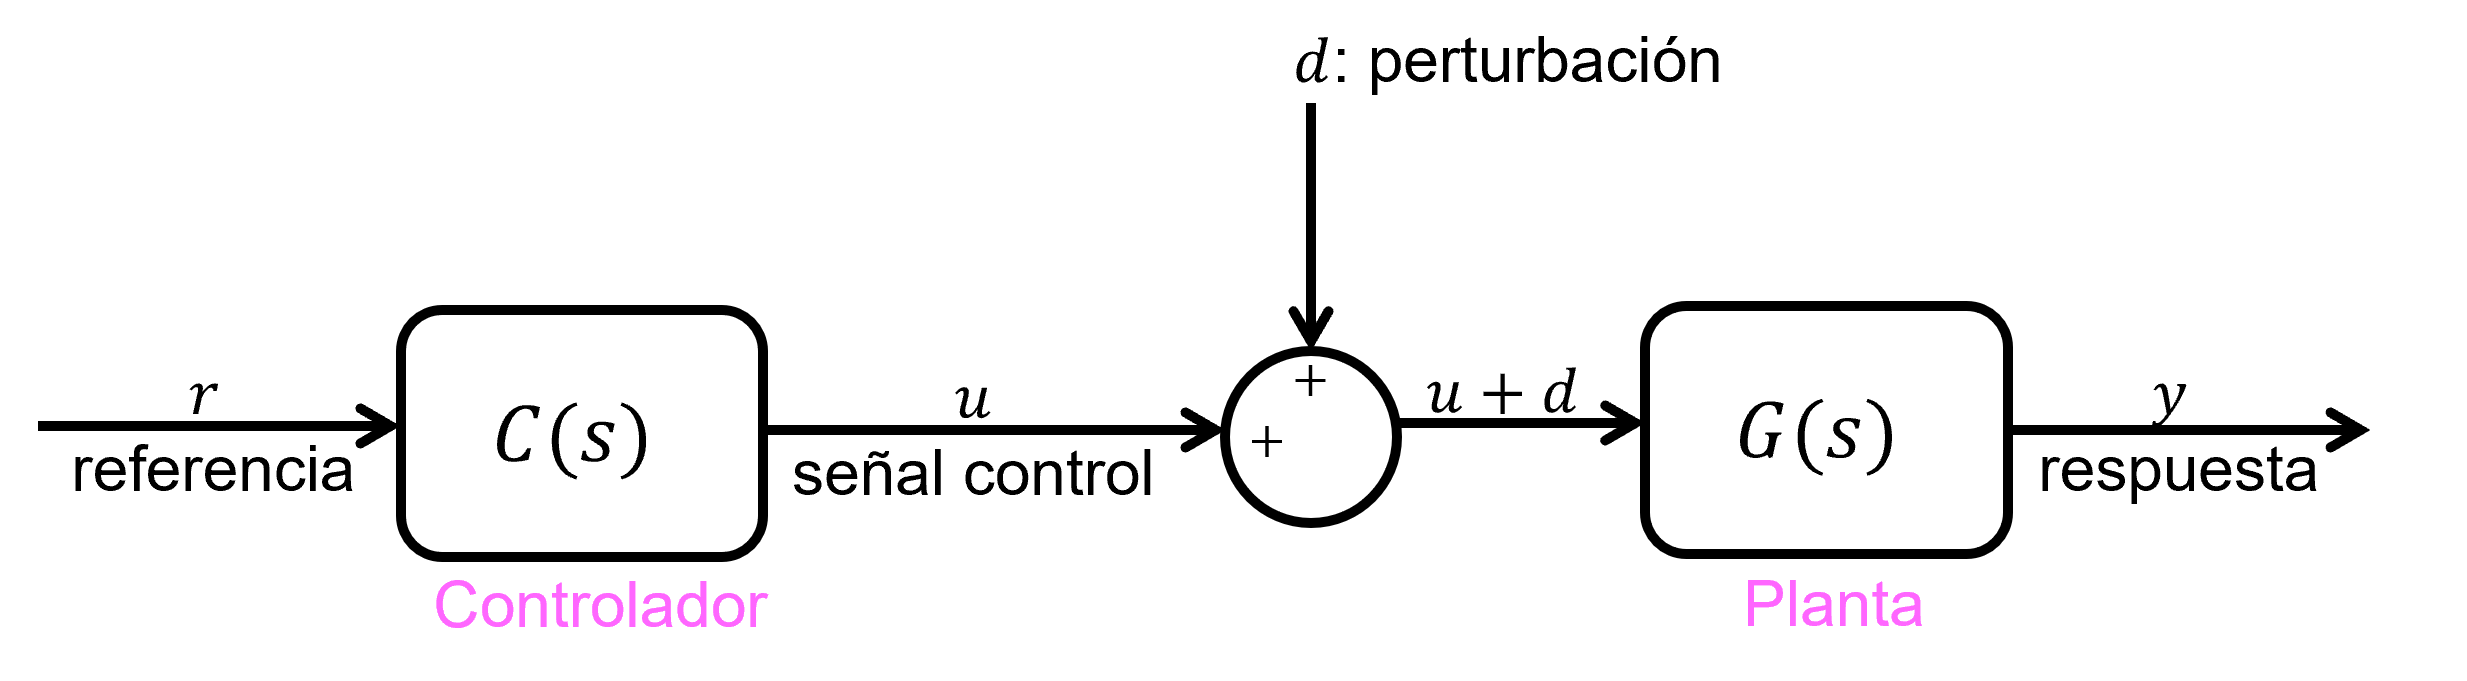
\includegraphics[scale=0.7]{Figuras/open-loop.png}
\end{figure}

\begin{itemize}
    \item[(1)] $Y(s)=G(s)[U(s)+D(s)]$, si asumimos $D(s)=0$
    \item[(2)] $U(s)=C(s)R(s)$
\end{itemize}

Reemplazar (2) en (1):
$$Y(s)=G(s)C(s)R(s)=L(s)R(s)$$
Donde $L(s)=G(s)C(s)$ es el sistema abierto ``open-loop system'' en representación función de transferencia.\\
\par Si buscamos: 
\begin{align*}
    y(t)&=r(t) ~/\mathcal{L}\{\cdot\}\\
    Y(s)&=R(s)\\
    \Longrightarrow L(s)&=1\\
    \Longrightarrow C(s)&=\frac{1}{G(s)} ~\text{``control inverso''}
\end{align*}

\underline{Nota}: 
\begin{itemize}
    \item Muy simple y ``barato'' (no hay necesidad de sensores)
    \item No es robusto $\Longrightarrow$ si hay incertidumbre en $G(s)$
    \begin{align*}
        L(s)&=G(s)C(s)\neq 1\\
        &=[\hat{G}(s)+\Delta(s)]\frac{1}{\hat{G}(s)}\\
        &=1+\frac{\Delta(s)}{\hat{G}(s)}
    \end{align*}
\end{itemize}
\underline{Nota}: podría ser útil en RTHS, porque la respuesta es instantánea.

\subsection{Closed-loop (feedback) control}
\begin{figure}[H]
\centering
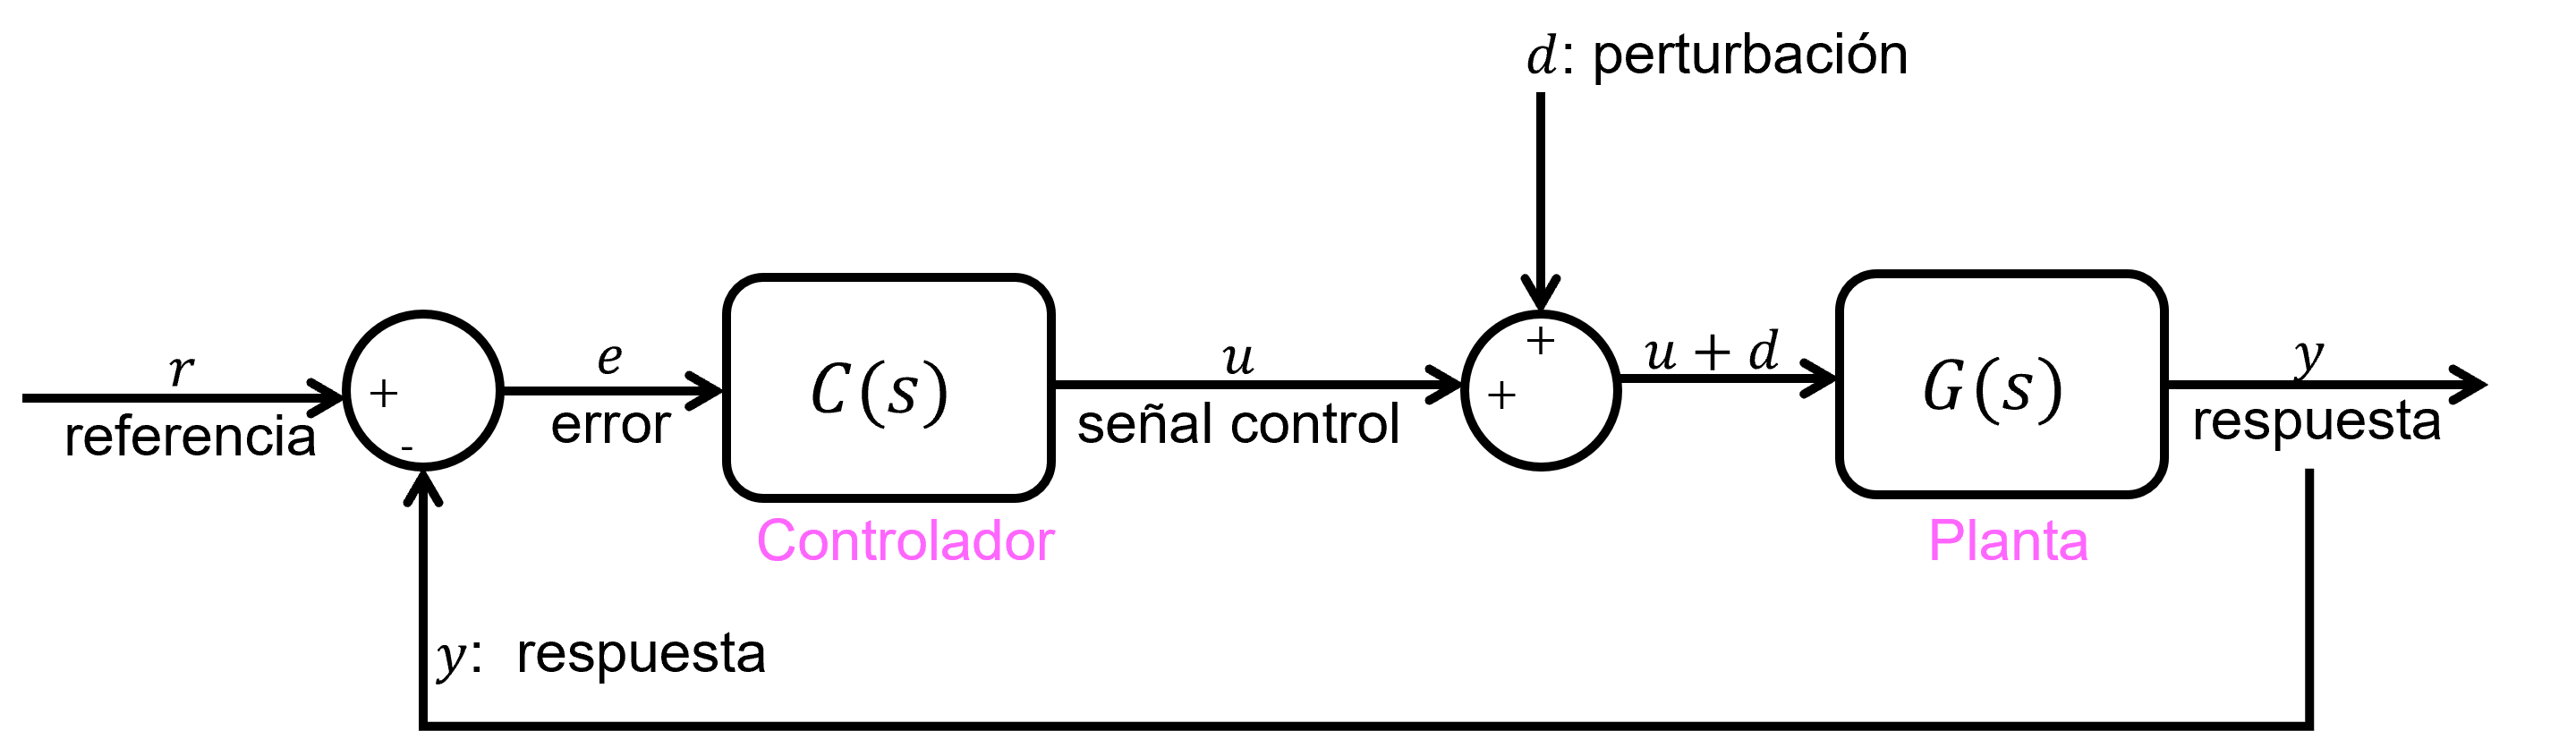
\includegraphics[scale=0.7]{Figuras/closed-loop.png}
\end{figure}

\begin{align*}
    \Longrightarrow & \text{Error: }~e(t)=r(t)-y(t)\\
    & \text{Si }e(t)=0\longrightarrow y(t)=r(t)
\end{align*}

\underline{Nota}:
\begin{itemize}
    \item Más robusto que feedforward $\Longrightarrow$ instalar sensores y ``alimentar'' la información de respuesta al controlador
    \item Más complicada y cara que open-loop
    \item Puede causar sistema estable o inestable
    \item Respuesta va a ser lenta $\Longrightarrow$ Real-time hybrid simulation
\end{itemize}

\subsubsection{Diagrama de Bloque}
Cuando se añade un dispositivo de control al sistema dinámico estructural, se genera un nuevo sistema dinámico con propiedades distintas.

\begin{figure}[H]
\centering
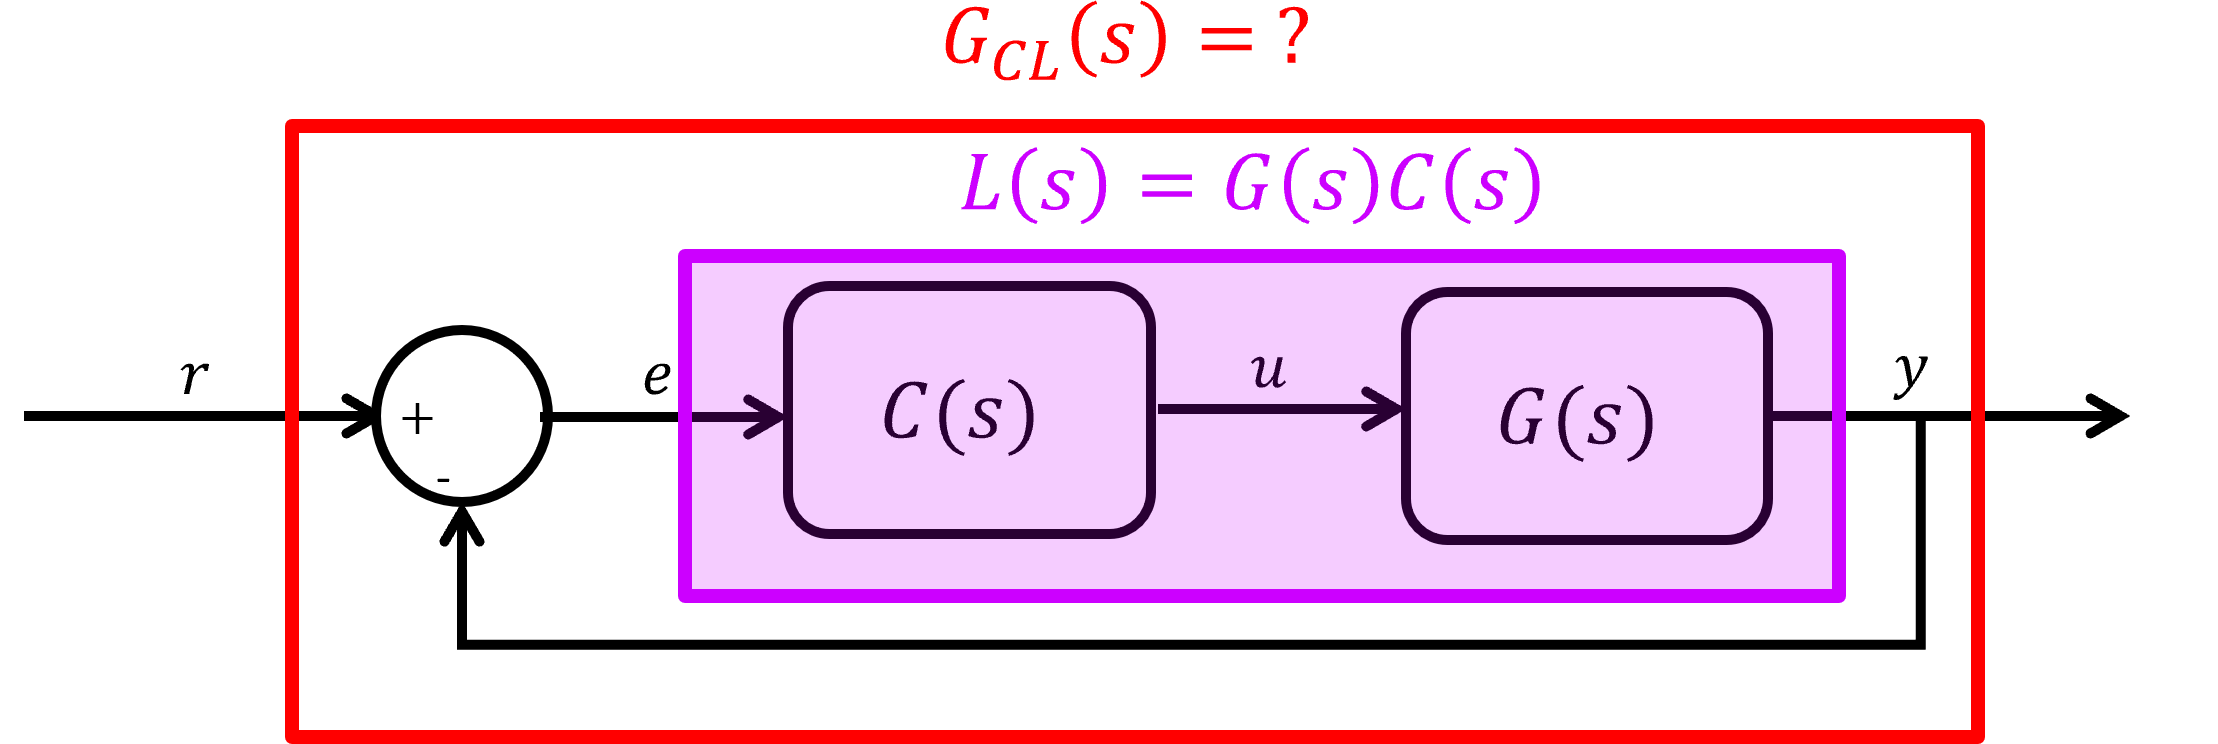
\includegraphics[scale=0.7]{Figuras/Diagrama_bloque.png}
\end{figure}

Desde el diagrama de bloques, se observa que:
\begin{align*}
    Y(s) = G(s)U(s)
\end{align*}

Pero, la señal de entrada $U(s)$ es la señal de salida del controlador:
\begin{align*}
    U(s) = C(s)E(s)
\end{align*}

Reemplazando, se obtiene que :
\begin{align*}
    Y(s) = G(s)C(s)E(s)
\end{align*}

Notar que la función de transferencia para este subsistema es $G(s)C(s)$. Siguiendo con el mísmo método reemplazando la señal de entrada por la multiplicación de su TF con su entrada (considerandola como salida):
\begin{align*}
    Y(s)&=L(s)E(s)=G(s)C(s)E(s)\\
    E(s)&=R(s)-Y(s)
\end{align*}

Reemplzando (2) en (1): 
\begin{align*}
    \Longrightarrow Y(s)&=G(s)C(s)[R(s)-Y(s)]\\
    \Longrightarrow[1+G(s)C(s)]Y(s)&=G(s)C(s)R(s)\\
    \Longrightarrow Y(s)&= \bigg[\frac{G(s)C(s)}{1+G(s)C(s)}\bigg]R(s)\\
    \Longrightarrow Y(s)&= G_{CL}(s)R(s)
\end{align*}

$\therefore G_{CL} = \bigg[\frac{G(s)C(s)}{1+G(s)C(s)}\bigg]$ es la función de transferencia del nuevo sistema que incorpora al controlador.

% \underline{Nota}: Vamos a ajustar $C(s)$ tal que $G_{CL}(s)$ tenga las propiedades deseadas en función de $t_r$, $M_p$ y $t_s$. O bien, elegir posición de los polos de $G_{CL}(s)$.

\section{Sistema estructural con Active Mass Damper (AMD)}
\begin{figure}[H]
\centering
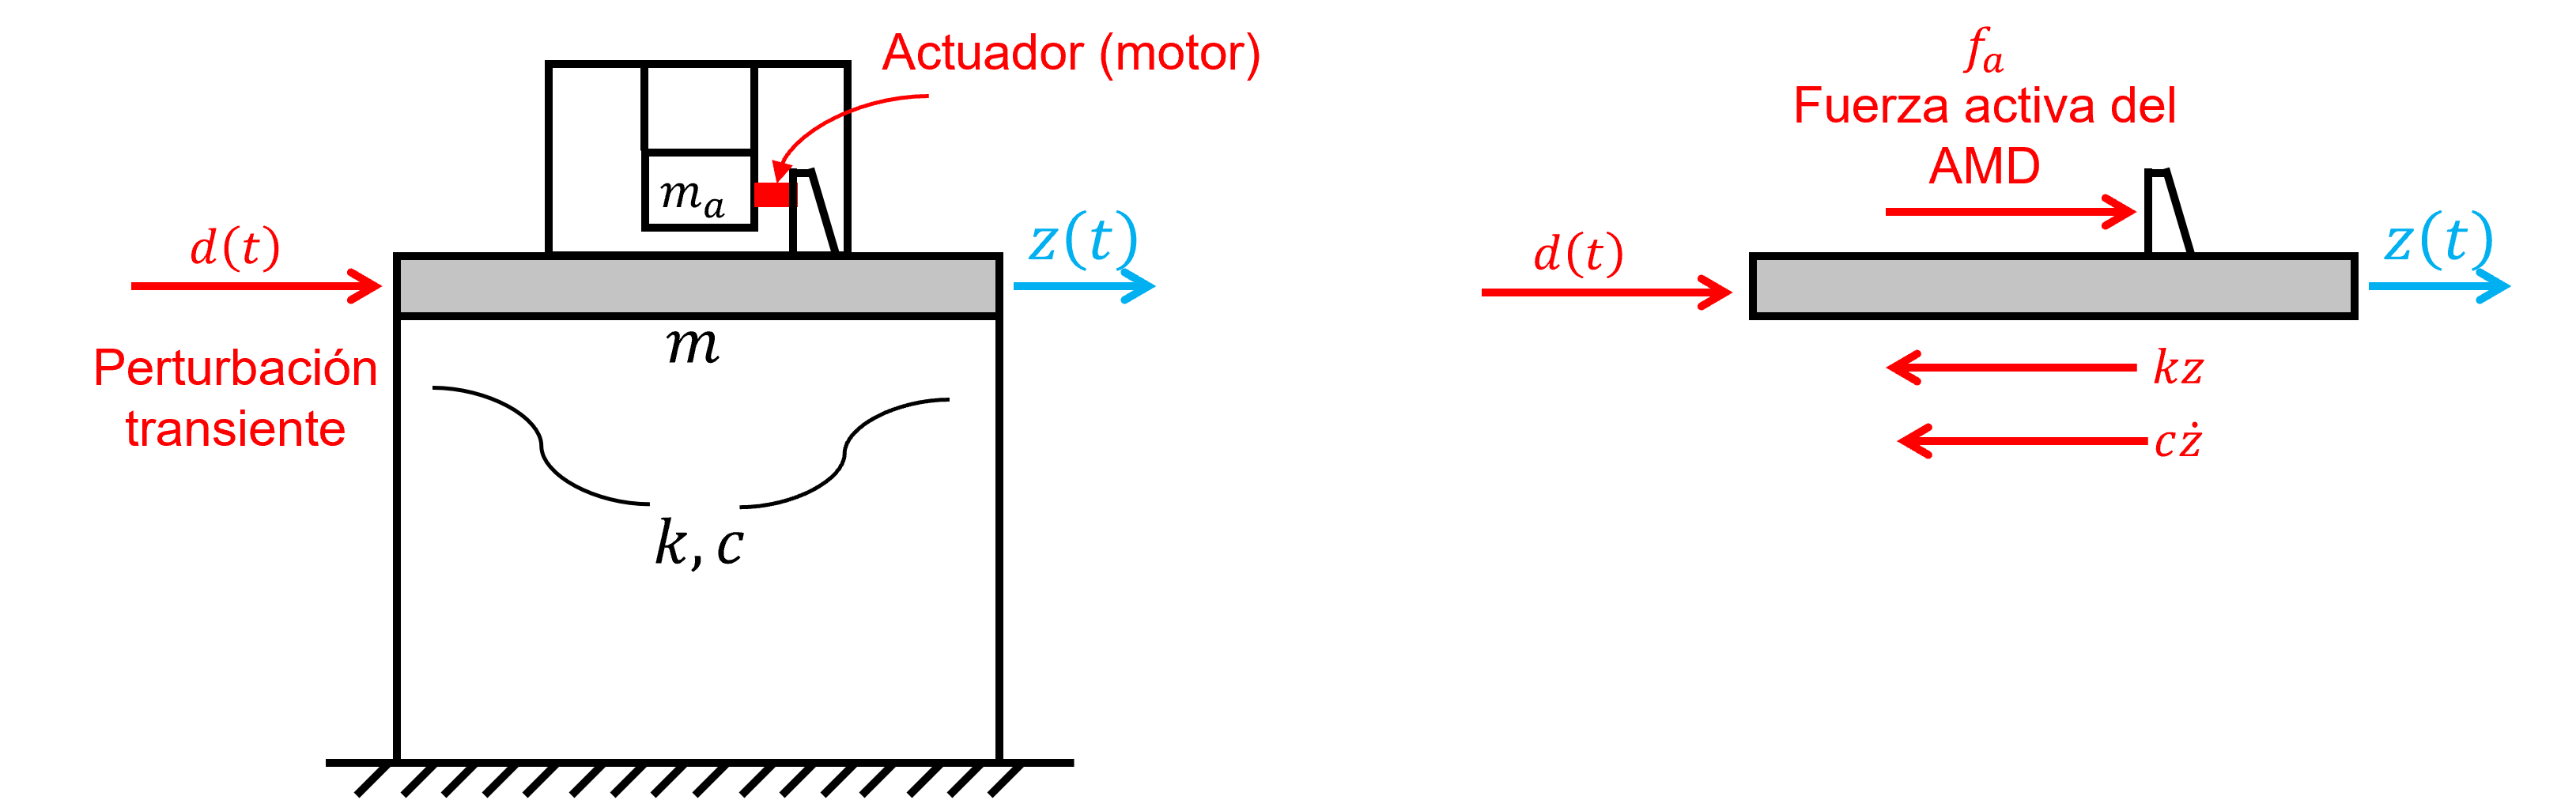
\includegraphics[scale=0.6]{Figuras/AMD.png}
\end{figure}
\begin{align*}
    \text{EDM: }~ m\ddot{z}+c\dot{z}+kz=f_a(u)+\cancelto{\text{Asuma=0}}{d}
\end{align*}
$u$: señal control (voltaje)\\
El objetivo es diseñar un \underline{algoritmo de control} $f_a(u,t)$ para mitigar $z(t)$ y mejorar el desempeño.


% \section{Respuesta transiente}
% Si queremos transicionar de un estado $x(t_0)$ a $x_2$, la respuesta no es instantánea y existe una respuesta transiente que hay que limitar.
% \begin{figure}[H]
% \centering
% 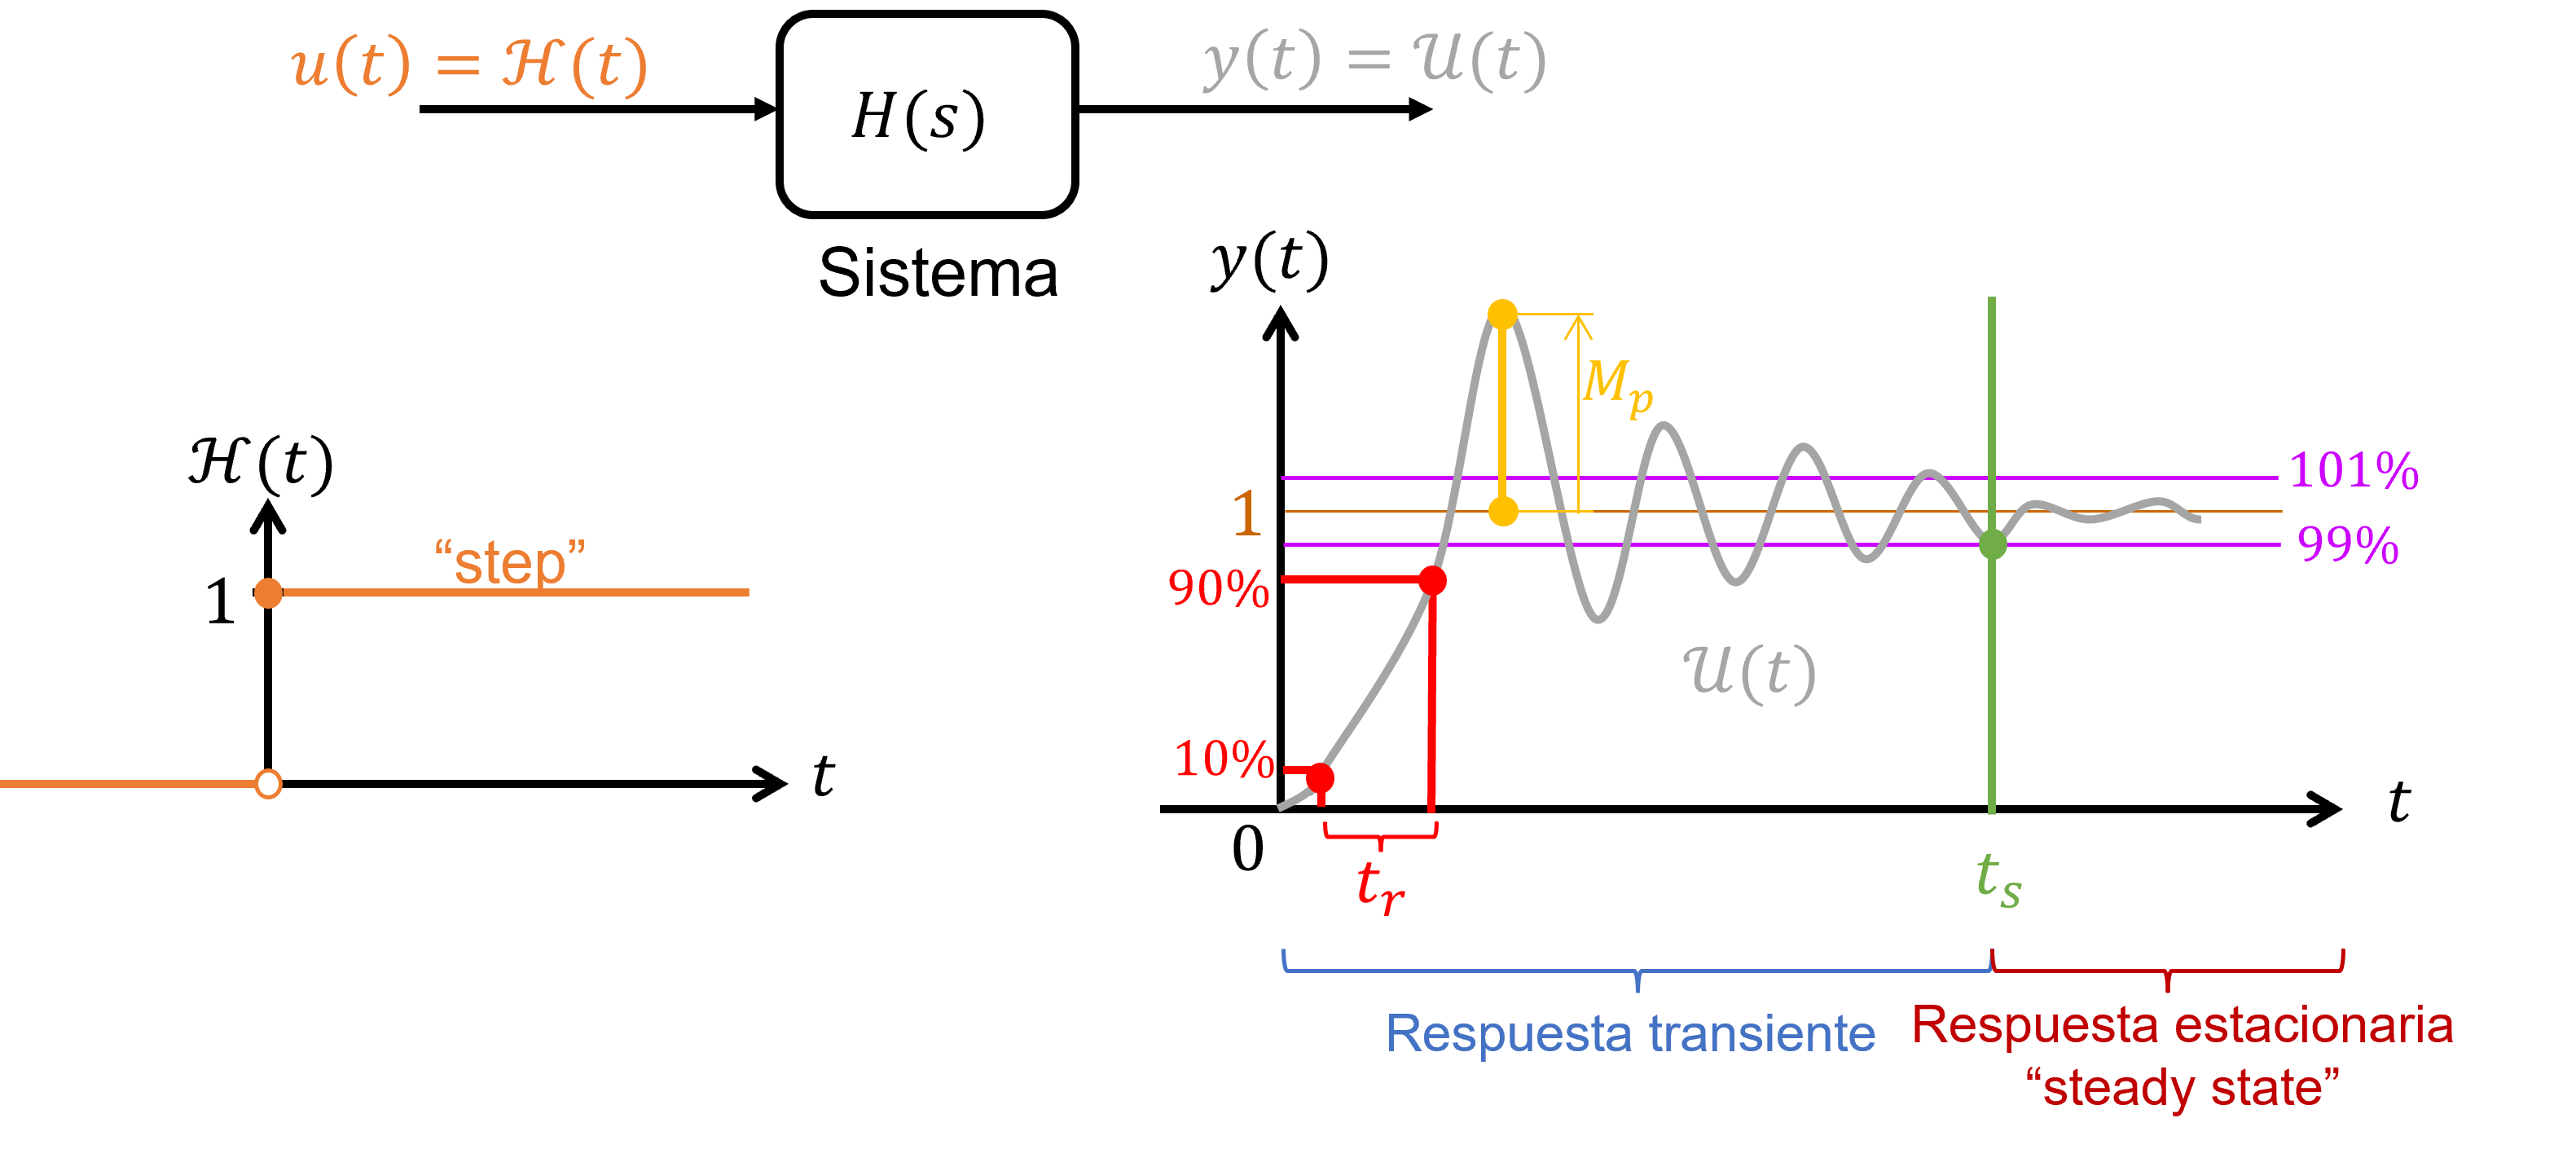
\includegraphics[scale=0.6]{step.png}
% \end{figure}
% \underline{Definición}:
% \begin{itemize}
%     \item \underline{Tiempo de subida} (``rise time'', $t_r$): tiempo que toma subir. Ej.: ir desde 10\% hasta 90\% de respuesta o de 0\% a 100\%.
%     \item \underline{Sobreimpulso} (``overshoot'', $M_p$): exceso de respuesta transitoria sobre la referencia deseada.
%     \item \underline{Tiempo de asentamiento} (``senttling time'', $t_s$): tiempo que toma el sistema en decaer hasta 1\%
% \end{itemize}

\section{Teorema del Límite Final}
\begin{figure}[H]
\centering
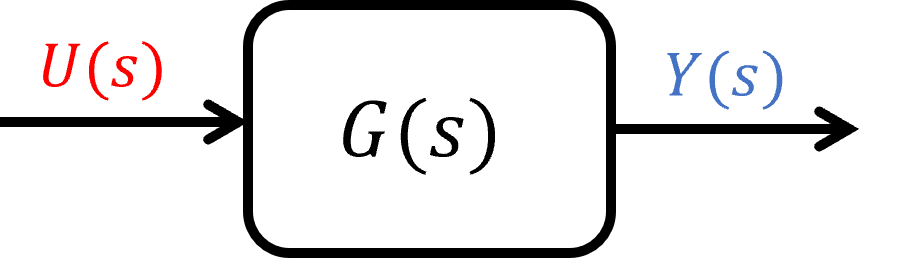
\includegraphics[scale=0.7]{Figuras/planta2.png}
\end{figure}
Respuesta Estado Estacionario: $y_\infty=\lim_{t\to\infty} y(t)$\\
\par Válido si y solo si $G(s)$ es estable.\\
\par \underline{Teorema}: Si todos los polos de $G(s)$ se encuentran a la izquierda del plano complejo, entonces:
\begin{align*}
    \lim_{t\to\infty} y(t)=\lim_{s\to 0} sY(s)
\end{align*}


\section{Requisitos de control}
\begin{figure}[H]
\centering
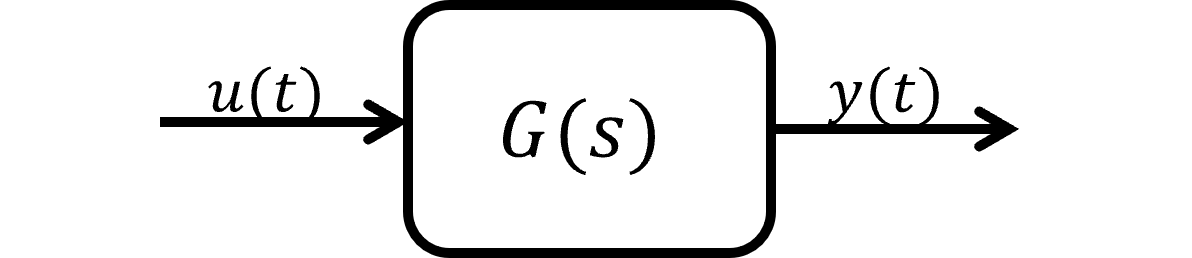
\includegraphics[scale=0.7]{Figuras/Planta.png}
\end{figure}
$\Longrightarrow$ Generar un set de requisitos de respuesta de planta $\Longrightarrow$ Especificaciones de respuesta transiente ante un escalón unitario
\begin{itemize}
    \item $t_r$ (tiempo de subida)
    \item $M_p$ (sobreimpulso)
    \item $t_s$ (tiempo de asentamiento)
\end{itemize}

\subsection{Especificaciones de Respuesta Transiente}

Ref: \textcite[Sec. 3.4]{Franklin2015}

Suponiendo un sistema LTI-SISO de segundo orden:\\

\begin{align*}
    \text{EDM: }~ m\ddot{u}+c\dot{u}+ku &= f\\
    \Longrightarrow H_{UF}(s) &= \frac{1/m}{s^2+2\zeta\omega_n s+\omega_n^2}
\end{align*}

Polos del sistema:

\begin{align*}
    s_{1,2} &= -\underbrace{\zeta \omega_n}_{\sigma} \pm j \underbrace{\omega_n \sqrt{1 - \zeta^2}}_{\omega_d} \\
    &= - \sigma \pm j \omega_d
\end{align*}

\begin{figure}[H]
    \centering
    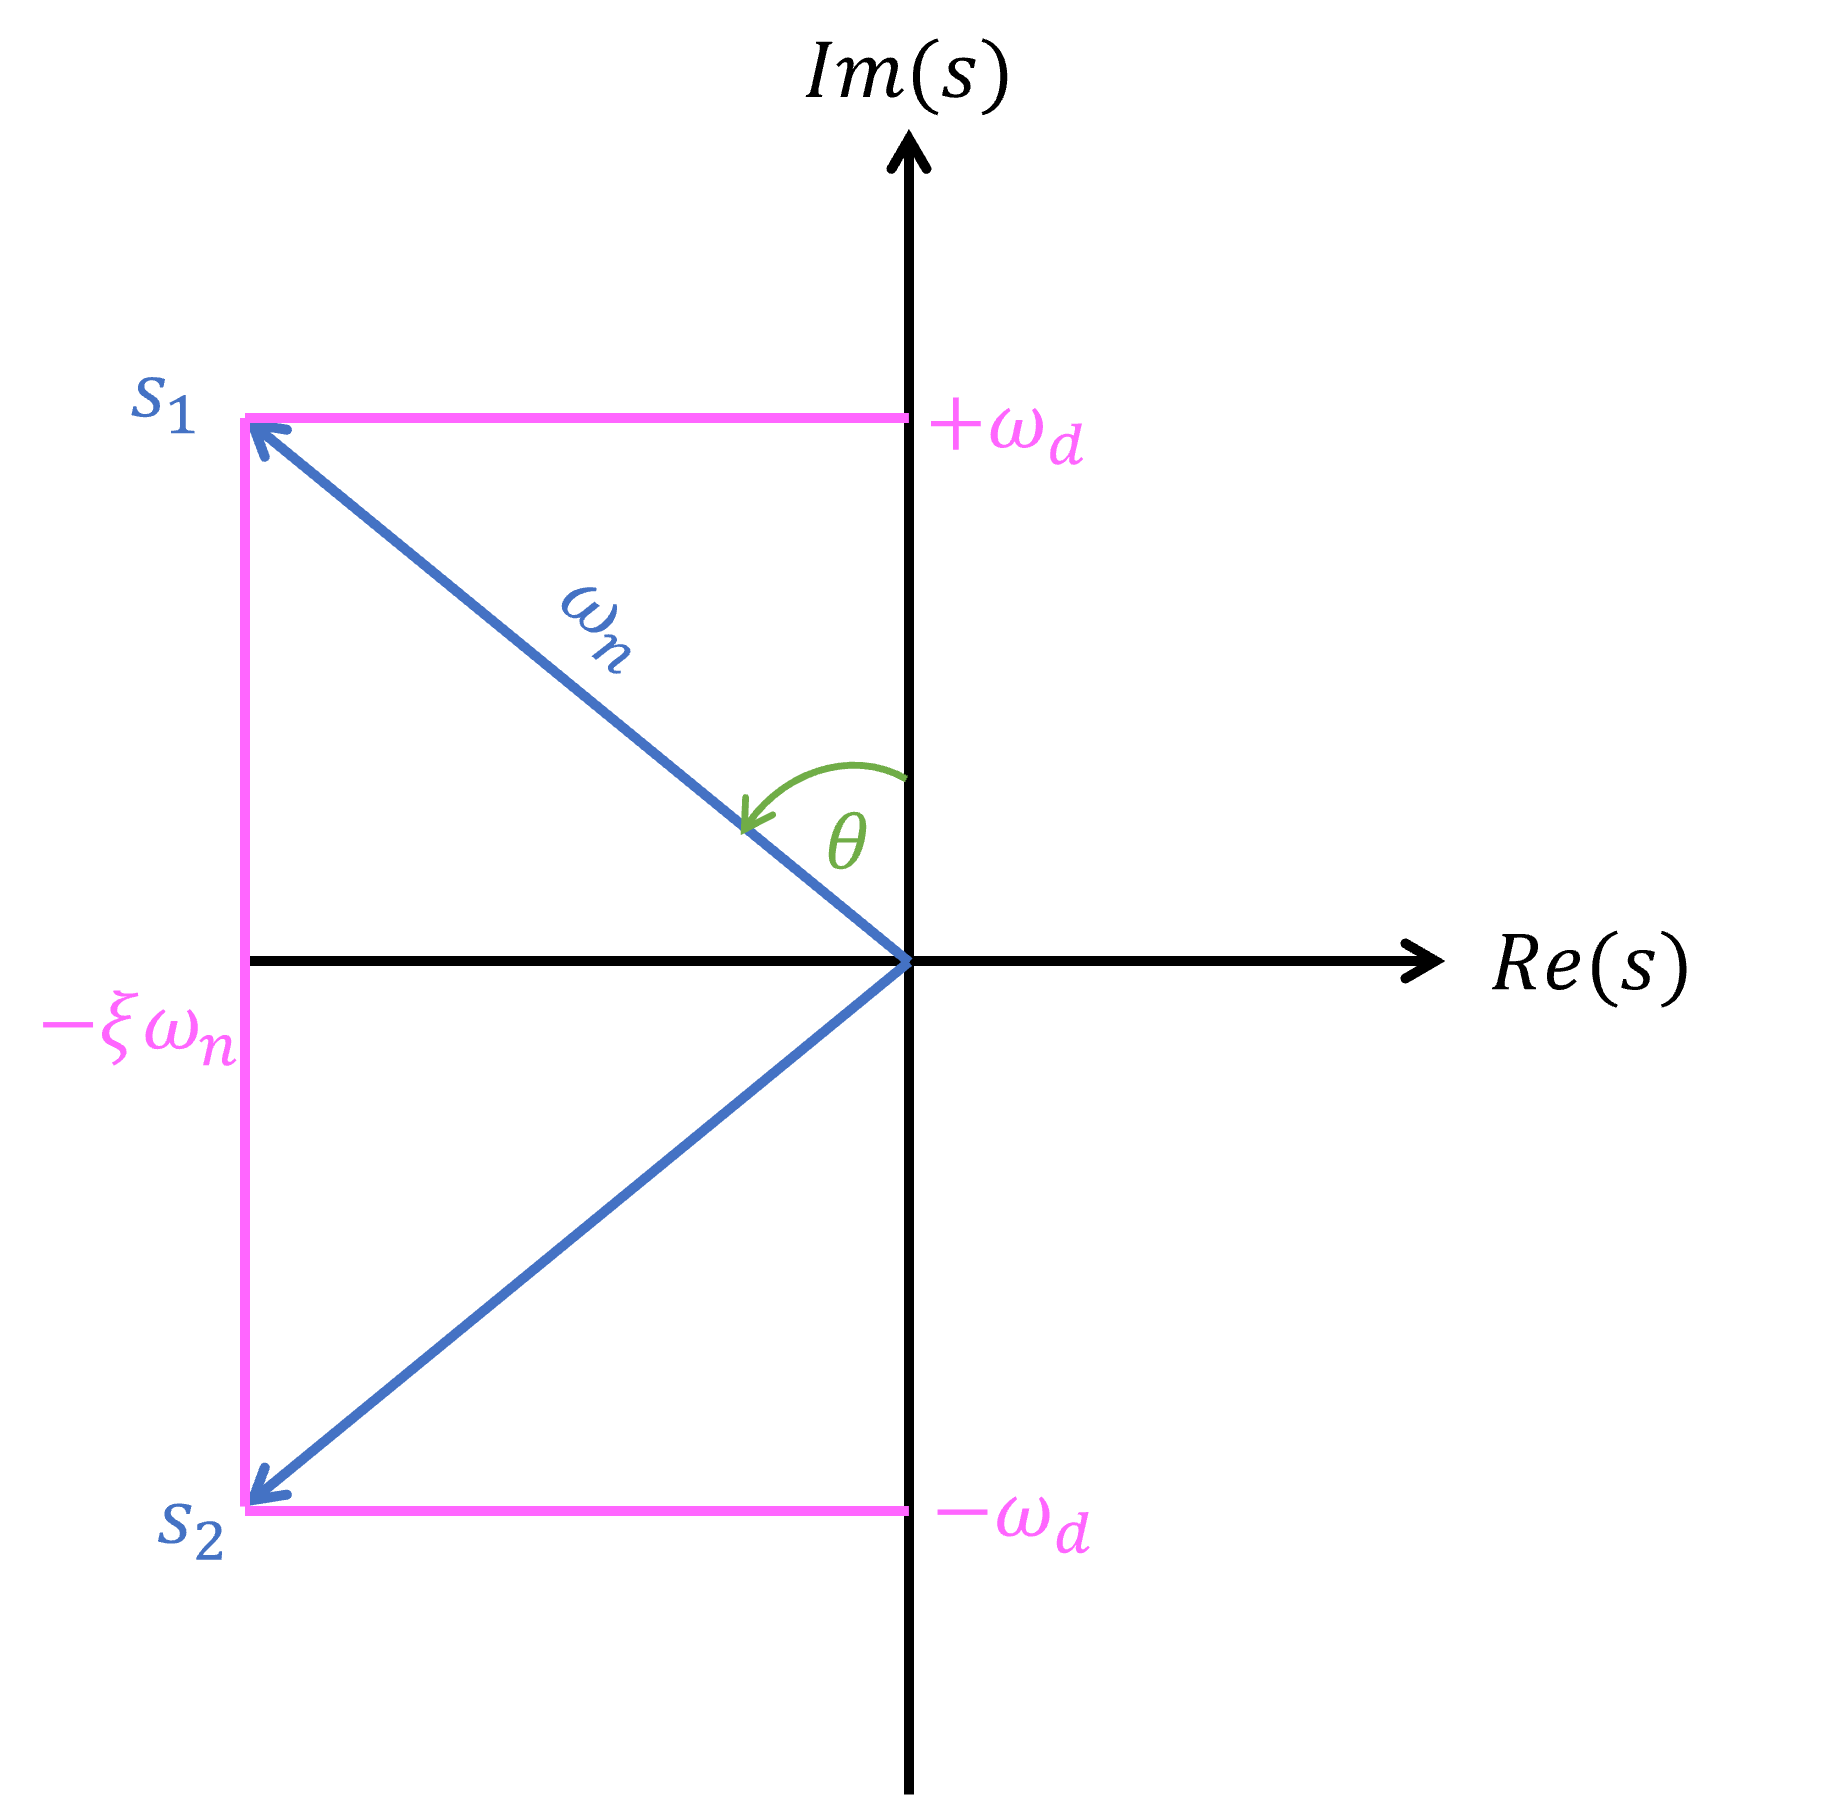
\includegraphics[scale=0.5]{transiente.png}
\end{figure}



Fórmulas para estimar la respuesta transiente para el caso de excitación escalón:

% Nota: Estas formulas son distintas a las descritas en la literatura para $\zeta = 50\%$, ver libro Franklin "Feedback Control"

\begin{itemize}
    \item \underline{Tiempo subida, $t_r$}: Asumiento $\zeta=2\%$, 
    $$t_r\approx \frac{1.6}{\omega_n}$$
    \item \underline{Sobreimpulso, $M_p$}: 
    $$-\log \left(\frac{M_p}{\pi} \right) \approx \tan(\theta)$$
    \item \underline{Tiempo asentamiento, $t_s$}: Asumiendo 2\% de respuesta esperada en ``steady-state'',
    $$t_s\approx \frac{4}{\zeta \omega_n} $$
\end{itemize}

\subsection{``Pole placement'', ubicación de polos}
Dadas las especificaciones transientes: $t_r$, $M_p$, $t_s$
\begin{align*}
    \color{VioletRed}{t_s}&<(t_s)_{lim}=\frac{4}{(\zeta\omega_n)_{lim}}\\
    \color{BurntOrange}{t_r}&<(t_r)_{lim}\approx \frac{1.6}{\omega_n}\\
    \color{LimeGreen}{M_p}&<(M_p)_{lim}=e^{-\pi\tan(\theta)}
\end{align*}

\begin{figure}[H]
\centering
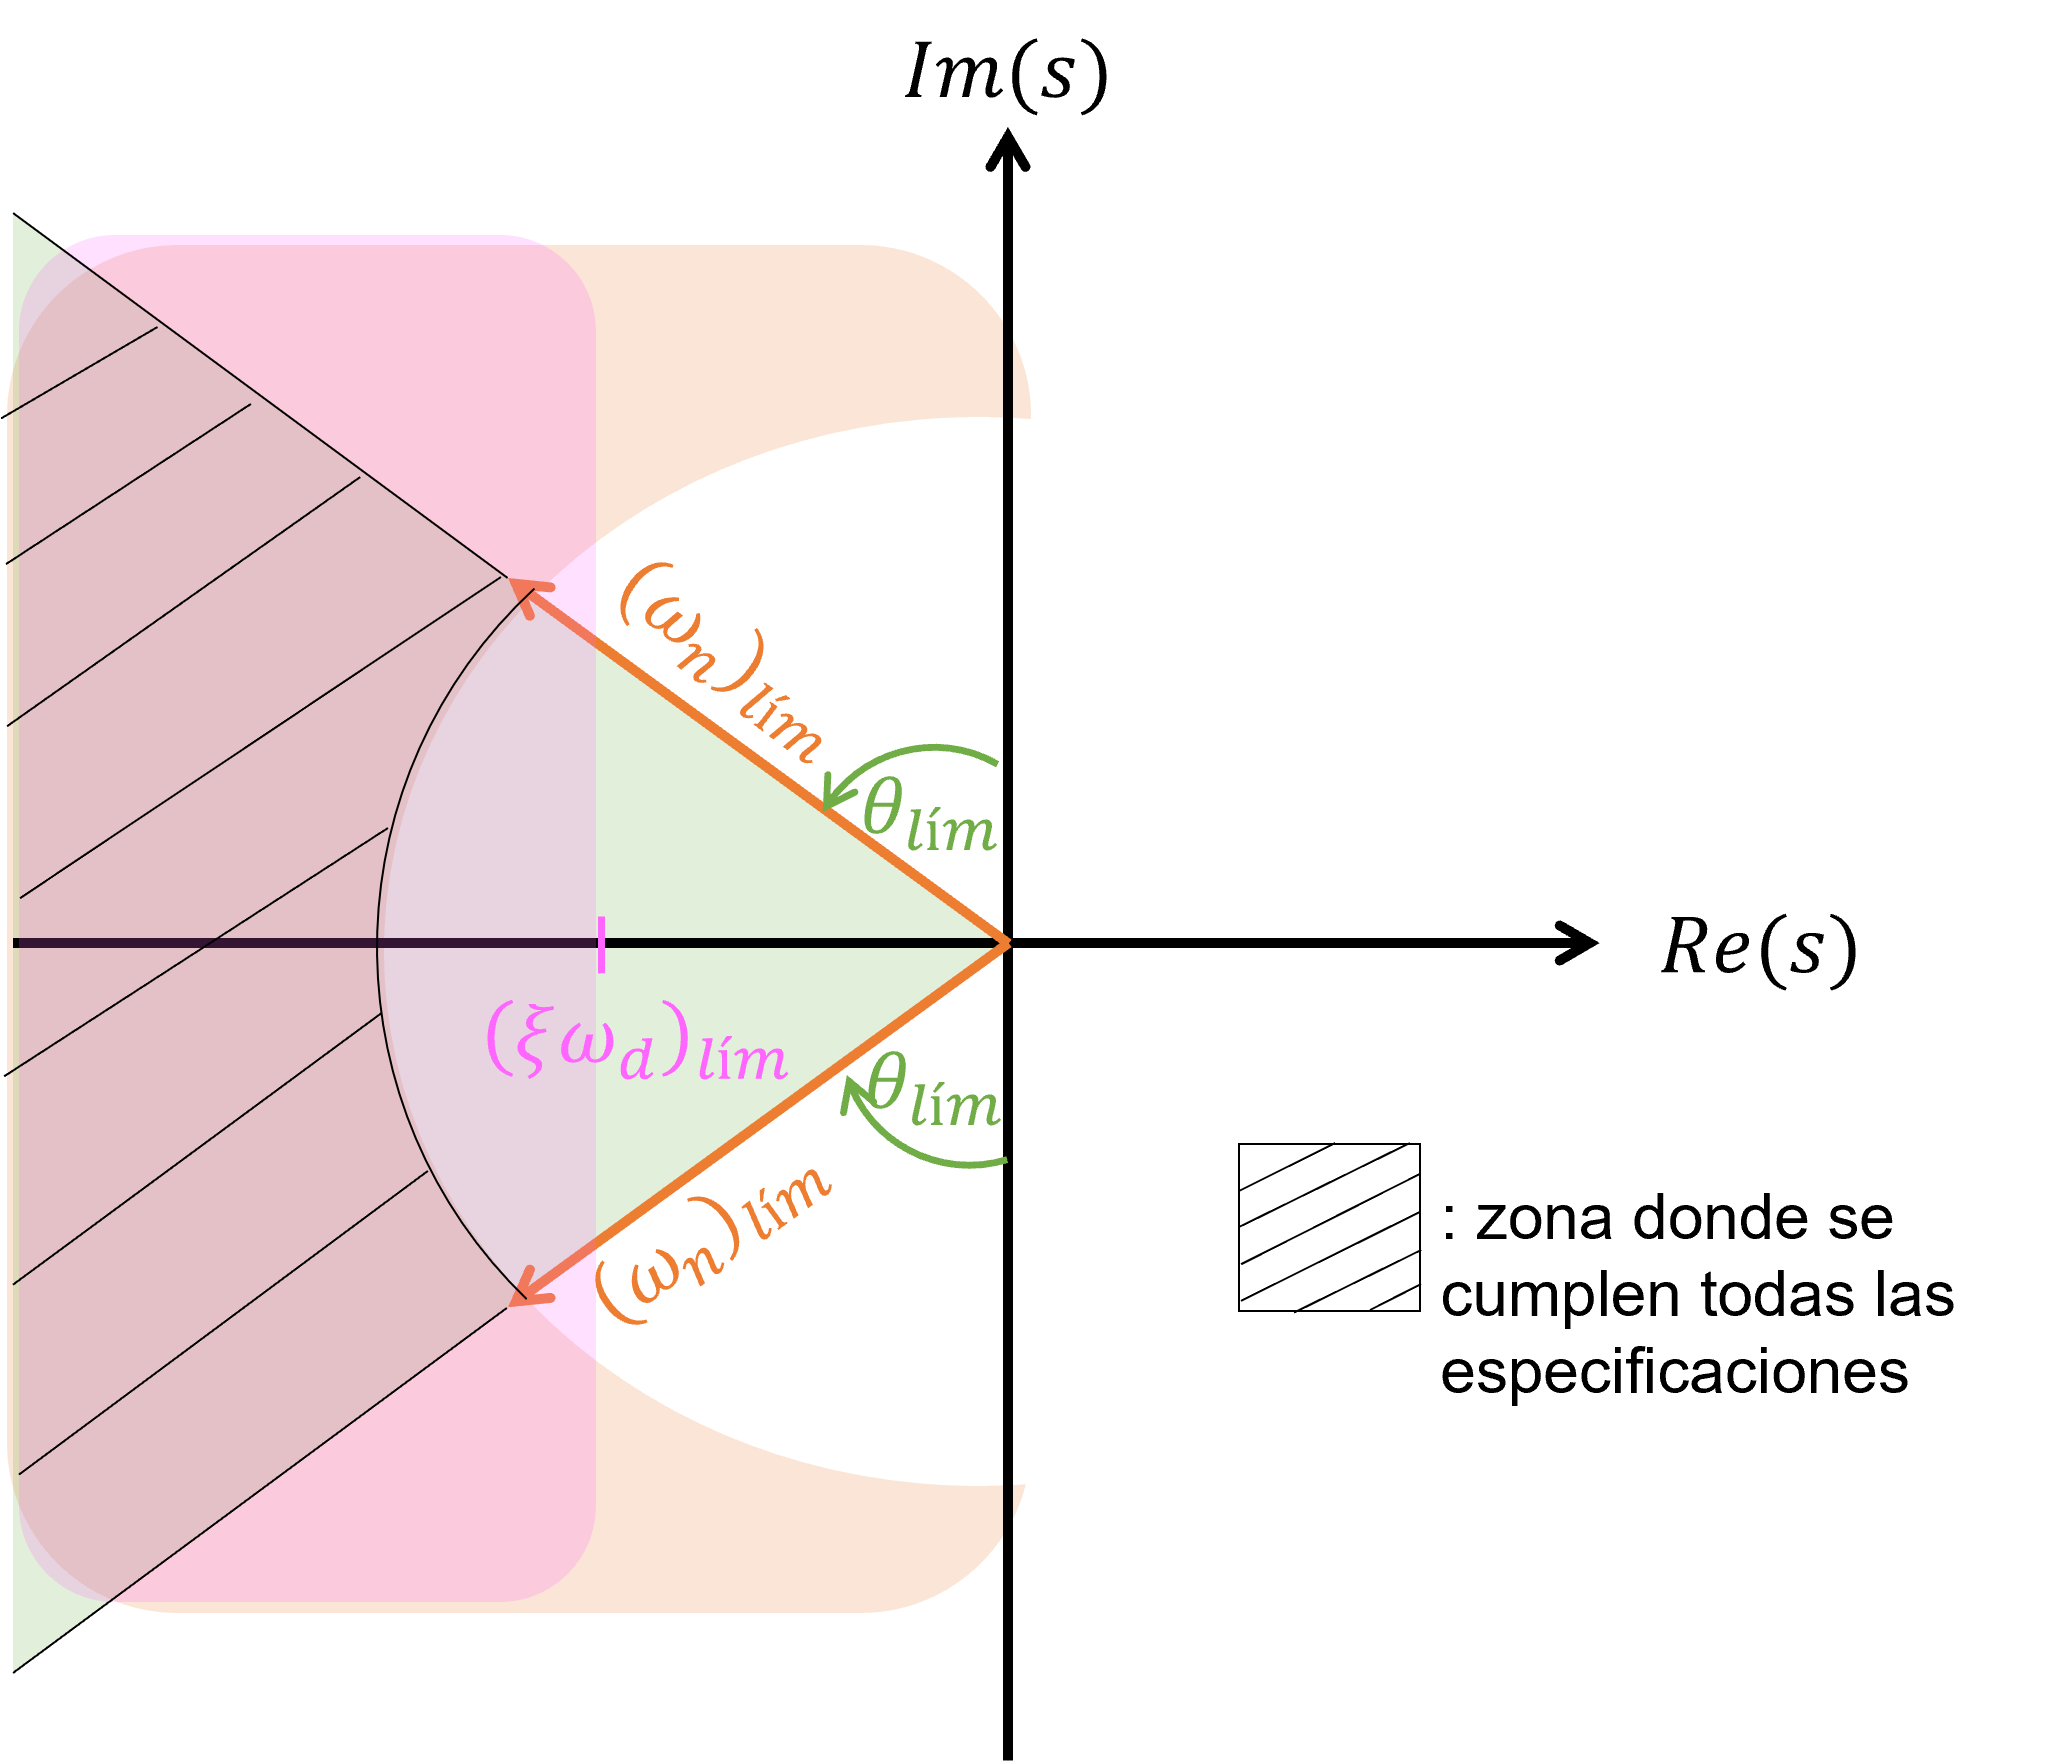
\includegraphics[scale=0.7]{pole_placement.png}
\end{figure}


\section{Control PID}
El control PID es un \underline{algoritmo de control} para diseñar la señal de control $u(t)$ para definir nuestra fuerza de control $f_a(u,t)$ es el control PID.
\begin{align*}
    u(t)&=K_pe(t)+K_D\frac{de(t)}{dt}+K_I\int e(t)dt\\
    \Longleftrightarrow U(s) &= K_pE(s)+K_DsE(s)+K_I\frac{E(s)}{s} \\
    \Longleftrightarrow U(s) &= \left(K_P + K_Ds + \frac{K_I}{s}\right)E(s)
\end{align*}

Si definimos $C(s) = K_P + K_Ds + \frac{K_I}{s}$
\begin{align*}
    U(s) = C(s)E(s)
\end{align*}
\begin{itemize}
    \item $K_p$: control proporcional
    \item $K_D$: control derivativo
    \item $K_I$: control integral
    \item $K_p e(t)$: error instantáneo
    \item $K_D \frac{de(t)}{dt}$: error futuro
    \item $K_I \int e(t) dt$: error pasado
    \item $e(t) = r(t) - y(t)$
\end{itemize}

\begin{figure}[H]
\centering
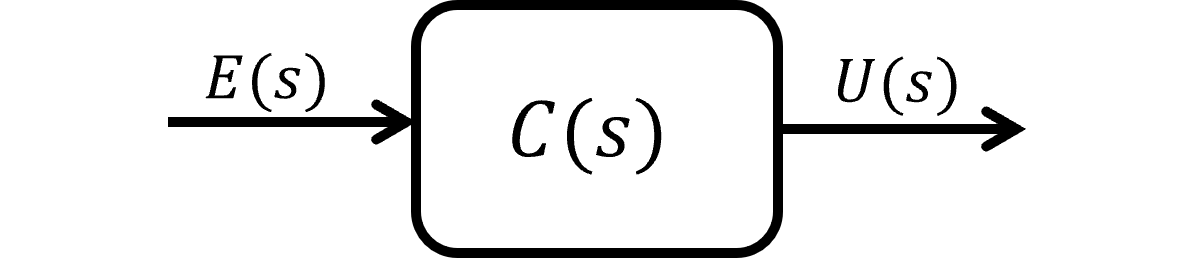
\includegraphics[scale=0.7]{Figuras/controlador.png}
\end{figure}

\begin{figure}[H]
\centering
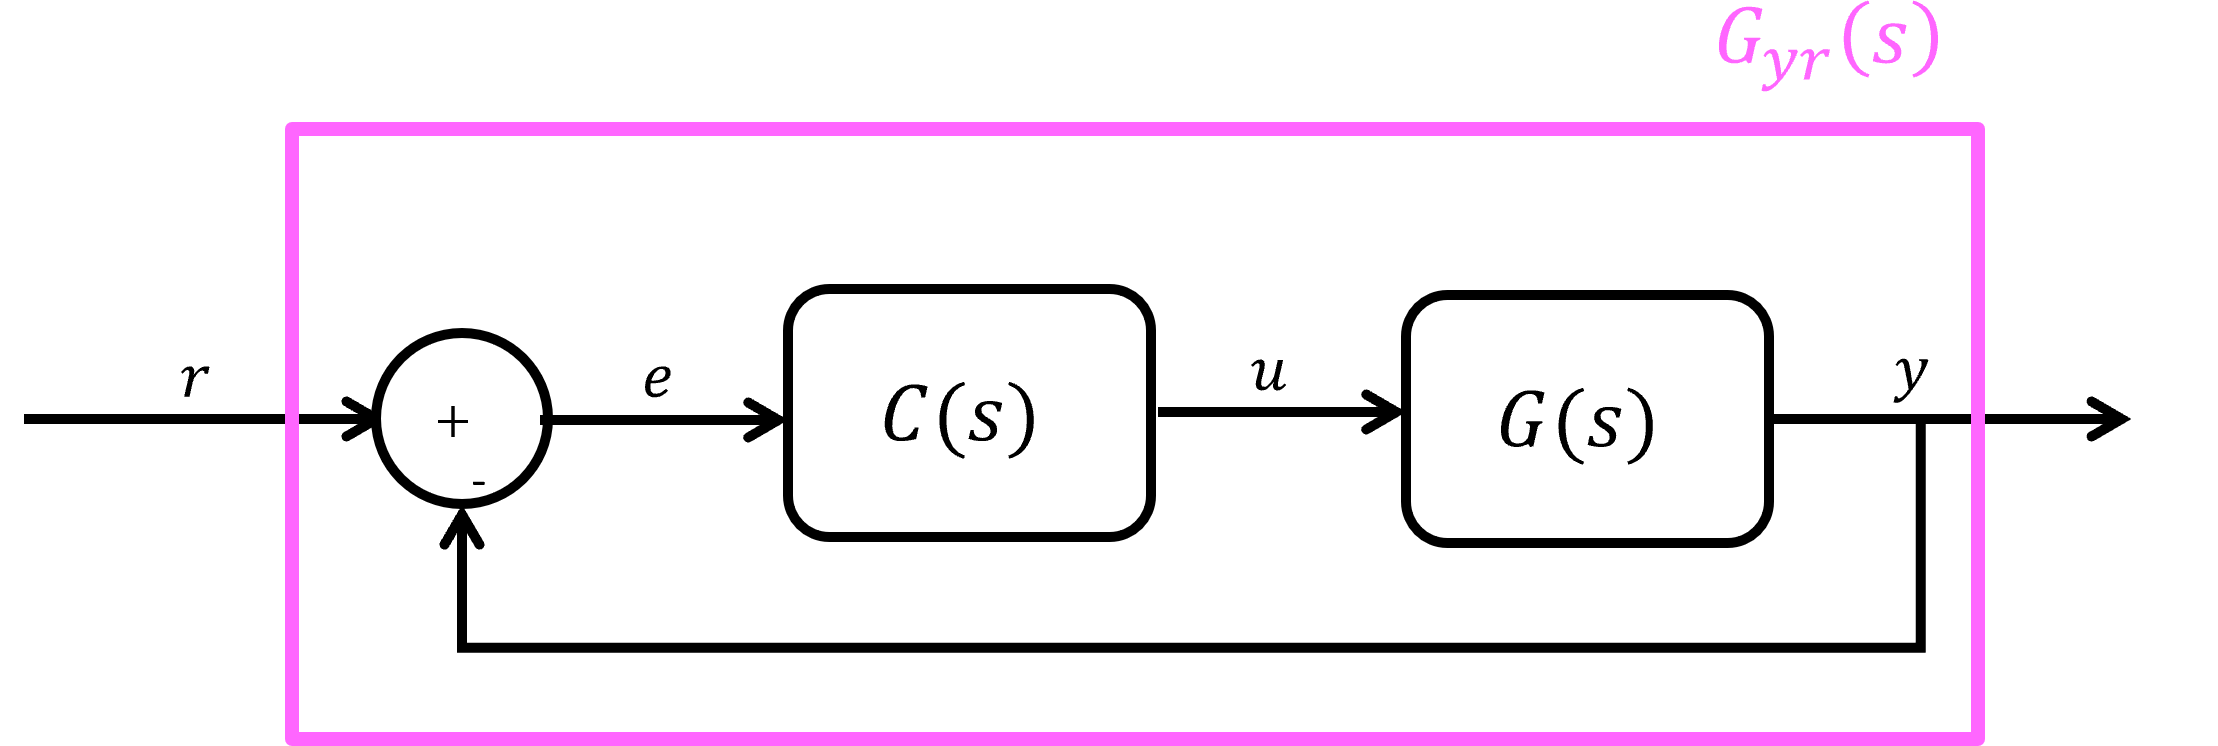
\includegraphics[scale=0.7]{Figuras/PID2.png}
\end{figure}
$C(s)$ se diseña tal que $e(t)\to 0$
$$C(s)=K_p+\frac{K_I}{s}+K_Ds$$
\begin{itemize}
    \item $Y(s)=G(s)U(s)$
    \item $U(s)=C(s)E(S)$
    \item $E(s)=R(s)-Y(s)$
\end{itemize}
\begin{align*}
    Y(s)&=G(s)C(s)[R(s)-Y(s)]\\
    \Longrightarrow Y(s)&=\frac{G(s)C(s)}{1+G(s)C(s)}R(s)\\
    &=G_{CL}R(s)\\
    &=G_{yr}R(s)
\end{align*}

\subsection{Control P}
Si se considera únicamente el control P (proporcional), se puede obtener la función de transferencia del sistema cerrado.
\begin{align*}
    & C(s)=K_p\\
    \Longrightarrow & G(s)=\frac{1}{ms^2+cs+k}=\frac{1/m}{s^2+2\zeta\omega_n s+\omega_n^2}=\frac{c}{s^2+as+b}\\
    \Longrightarrow & G_{CL}(s)=\frac{K_p\frac{c}{s^2+bs+c}}{1+K_p\frac{c}{s^2+bs+c}} \\
    \Longrightarrow & G_{CL}(s)=\frac{K_p c}{s^2+as+(b+K_p\cdot c)} \longrightarrow \text{Función de transferencia Closed-loop}
\end{align*}

Al tener la misma forma de un sistema 1GDL, se pueden definir propiedades equivalentes:
\begin{align*}
    \Longrightarrow & \omega_{n,CL}= \sqrt{b+K_p\cdot c}\\
    \Longrightarrow & \zeta_{CL}= \frac{a}{2\omega_{n,CL}}=\frac{a}{2\sqrt{b+K_p\cdot c}}
\end{align*}

Notar que:
\begin{itemize}
    \item Aumentar $K_p$ hace que $\omega_{n,CL}$ aumente (sistema rígido)
    \item Aumentar $K_p$ hace que $\zeta$ disminuya
\end{itemize}

En términos de la respuesta $y_{\infty}$: 
\begin{align*}
    y_{\infty}=\lim_{s\to 0}sY_{CL}(s)=\lim_{s\to 0} sG_{CL}(s)R(s)
\end{align*}
Con $R(s)$: escalón unitario

\begin{align*}
    \Longrightarrow y_{\infty}=\lim_{s\to 0} s\frac{K_p\cdot c}{s^2+as+(b+K_p\cdot c)}\cdot\frac{1}{s}=\frac{K_p\cdot c}{b+K_p \cdot c}\neq 1
\end{align*}
Valores pequeños de $K_p\Longrightarrow$ error en estado estacionario
\begin{figure}[H]
\centering
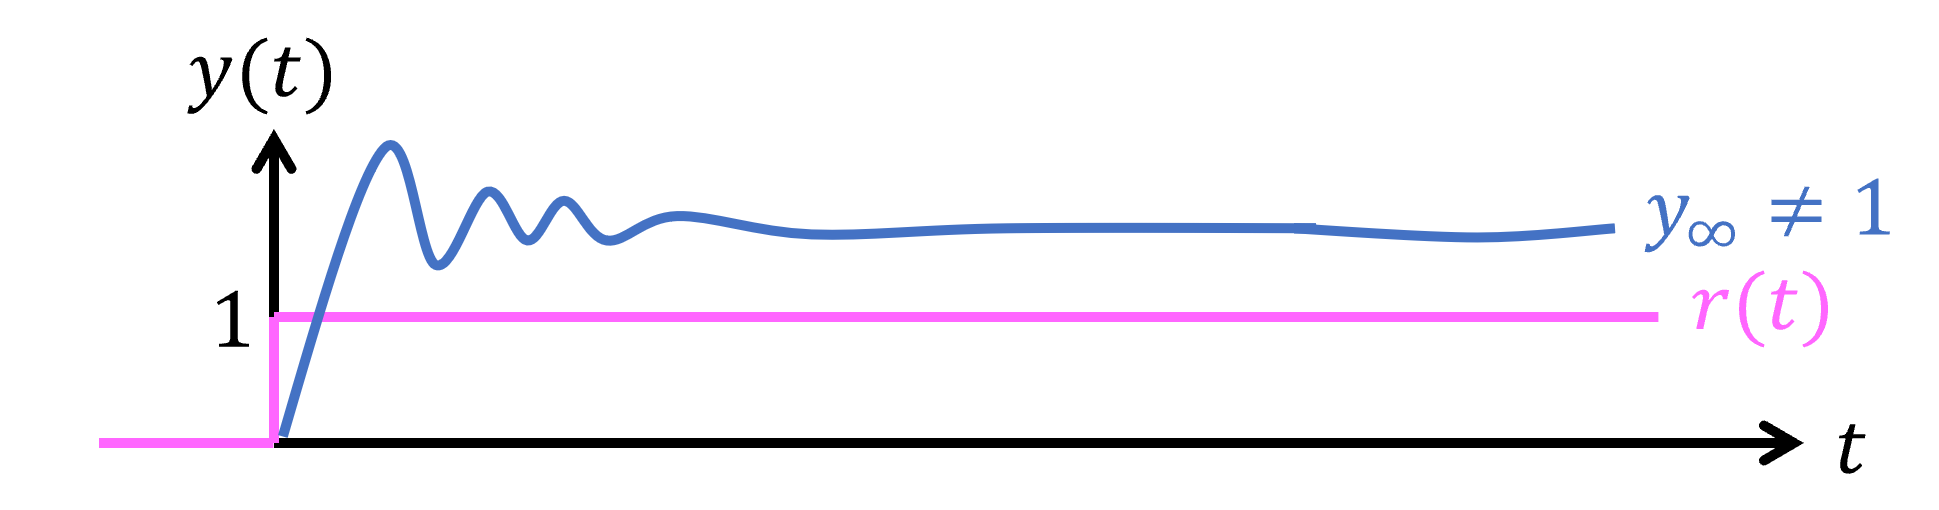
\includegraphics[scale=0.7]{Figuras/controlP.png}
\end{figure}

\subsection{Control PD}
Análogamente al control P, se puede obtener la función de transferencia de un sistema estructural con control PD
\begin{align*}
    G_{CL}(s)&=\frac{G(s)C(s)}{1+G(s)C(s)}=\frac{\left(\frac{c}{s^2+as+b}\right)C(s)}{1+\left(\frac{c}{s^2+as+b}\right)C(s)}\\
    & = \frac{c\cdot C(s)}{a^2+as+\left( b+c \cdot C(s) \right)}
\end{align*}

Si el controlador es PD, entonces se obtiene la expresión para el sistema cerrado:
\begin{align*}
    C(s) &= K_p+K_Ds=K_p(1+T_Ds)\\
    \Longrightarrow G_{CL} &= \frac{cK_p(1+T_Ds)}{s^2+(a+cbK_pT_D)s+b(1+K_p)}
\end{align*}

\begin{itemize}
    \item Aparece un ``cero'' en el numerador
    \item Podemos controlar $\omega_{n,CL}$ mediante $K_p$
    \item Podemos controlar $\zeta_{CL}$ mediante una combinación de $K_p$ y $T_D$
\end{itemize}

$\Longrightarrow y_{\infty}$, no hay cambio en el error de estado estacionario\\
\par $\Longrightarrow$ Con PD podemos ubicar los polos del sistema cerrado donde nosotros queramos\\
\par \underline{Advertencia}: Control D amplifica el ruido eléctrico en la señal de respuesta $\Longrightarrow$ Nunca utilizar control D.

\subsection{Control PI}
\begin{align*}
    \Longrightarrow G_{CL}(s) &= \frac{c\cdot C(s)}{s^2+as+\left(b+c \cdot C(s)\right)}\\
    \Longrightarrow C(s) &= K_p +\frac{K_I}{s}=K_P\left(1+\frac{T_I}{2}\right)\\
    \Longrightarrow G_{CL} &= \frac{cK_p(s+T_I)}{s^3+as^2+(b+cK_p)s+cK_pT_I}
\end{align*}

\begin{align*}
    \Longrightarrow y_{\infty}=\lim_{s\to 0}sY_{CL}(s)=\lim_{s\to 0} s\frac{K_p\cdot c(s+T_I)}{s^3+as^2+(b+cK_p)s+cK_pT_I}\cdot\frac{1}{s}=\frac{T_IK_p\cdot c}{T_IK_p\cdot c}= 1
\end{align*}

\underline{Nota}: El esfuerzo del control I genera una reducción del error en estado estacionario.

\subsection{Control PID}
\begin{align*}
    C(s) &= K_p+\frac{K_I}{s}+K_Ds\\
    &= K_p\left(1+\frac{T_I}{s}+T_Ds\right)
\end{align*}

\begin{itemize}
    \item Aumentar $K_p$: Sistema que responde rápido, pero se genera alto sobreimpulso, y el error estacionario alto.
    \item Aumentar $K_D$: Agregar amortiguameinto al sistema (disminuir sobreimpulso), pero puede amplificar el ruido eléctrico.
    \item Aumentar $K_I$: Reducir el error en estado estacionario, sistema se vuelve más lento.
\end{itemize}

\begin{table}[H]
    \centering
    \begin{tabular}{c|c|c|c|}
                & $K_p \uparrow$ & $K_D \uparrow$ & $K_I \uparrow$\\ \hline
         error ss & $\downarrow$ & - & 0\\ \hline
         $t_r$ & $\downarrow$ & - & ? \\ \hline
         $t_s$ & - & $\downarrow$ & ? ($\uparrow$)\\ \hline
         $M_p$ & $\uparrow$ & $\downarrow$ & ? ($\uparrow$)\\ 
    \end{tabular}
\end{table}



\section{Ejemplo: Simulación control PID mediante Simulink}
\begin{figure}[H]
\centering
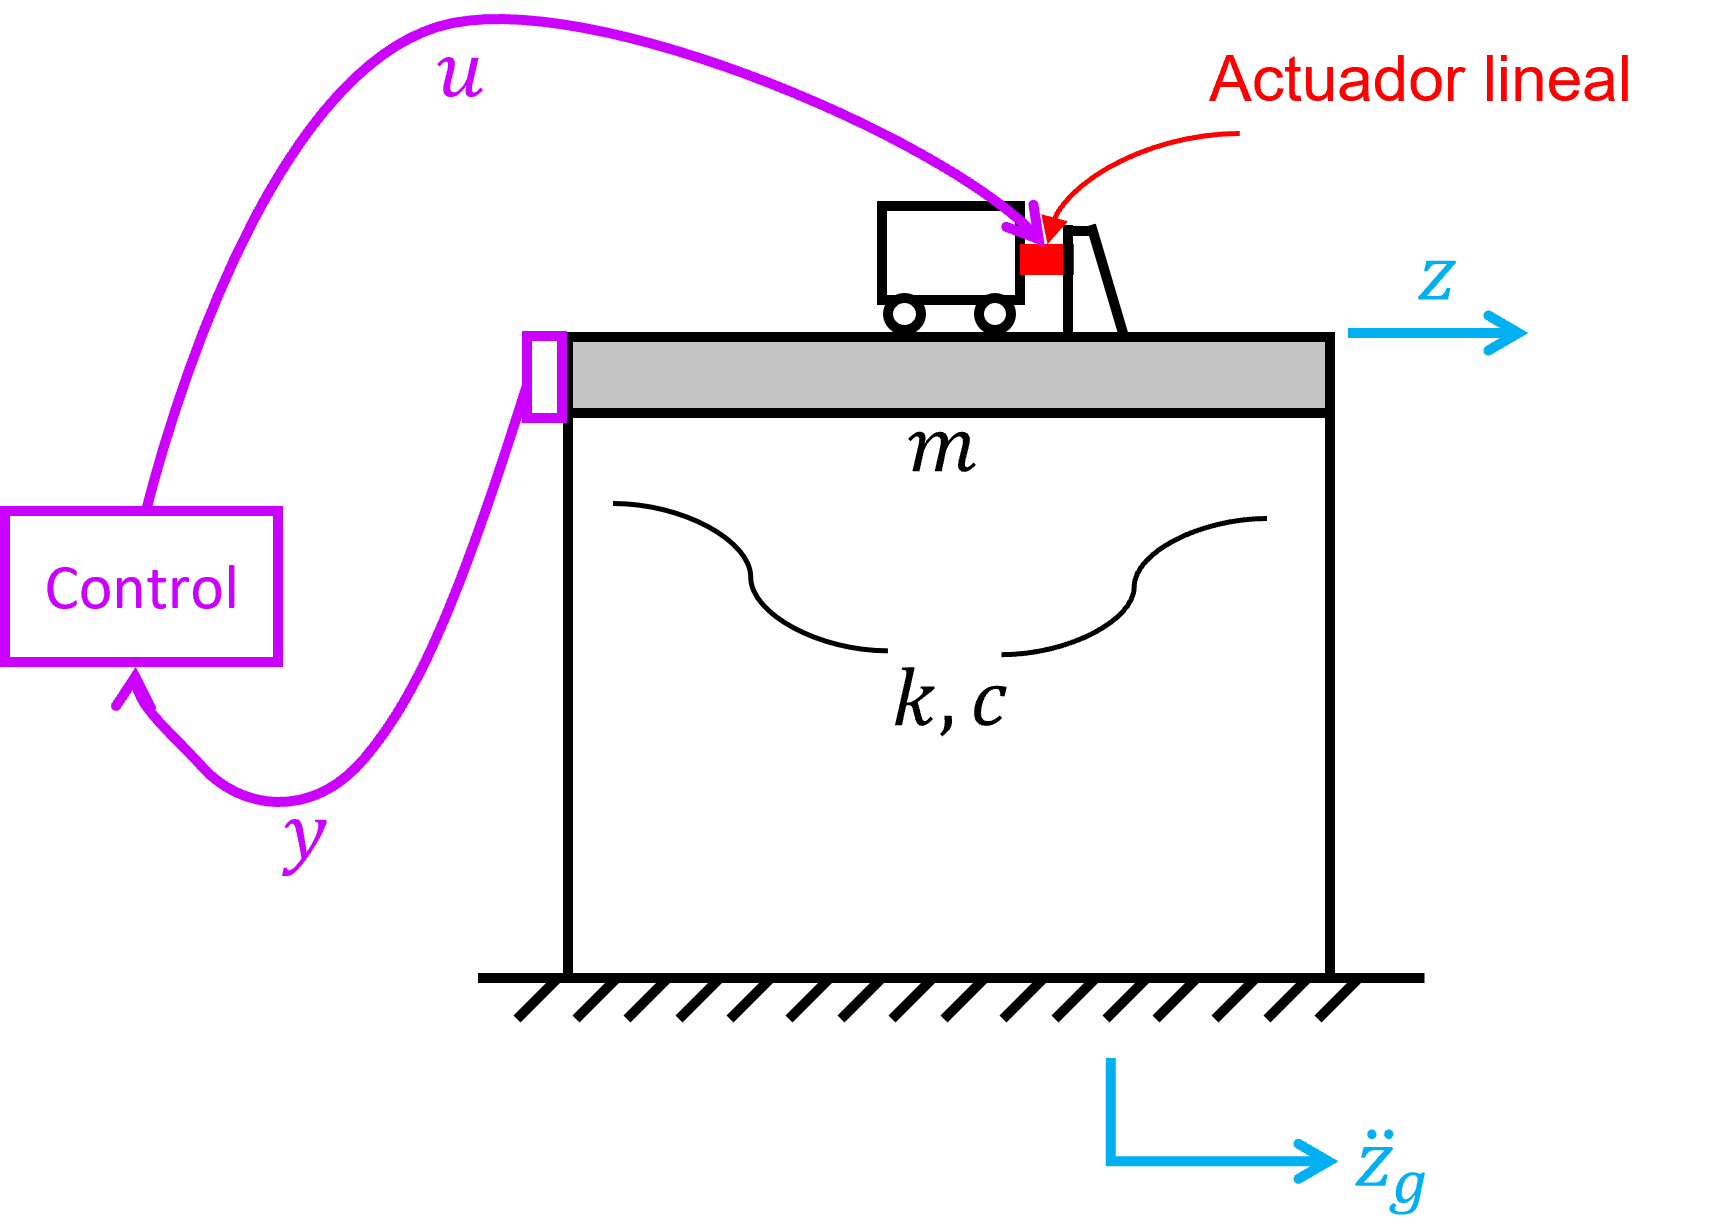
\includegraphics[scale=0.7]{Figuras/simulink_modelo.png}
\end{figure}

\begin{align*}
    \text{EDM: }~ m\ddot{z}+c\dot{z}+kz=-m\ddot{z}_g+gu
\end{align*}

\underline{Propiedades de la estructura}: 
\begin{itemize}
    \item $m=100$ Kg
    \item $c=50$ Ns/m
    \item $k=4000$ N/m
    \item $g=100$ N/V
\end{itemize}

\underline{Representación espacio-estado}: 
\begin{align*}
    {x}=\begin{bmatrix}{z}\\ {\dot{z}}\end{bmatrix}, \quad u_1 =\ddot{z}_g, \quad u_2=u
\end{align*}

\begin{align*}
    {\dot{x}} &=
    \begin{bmatrix}
    0 & 1\\
    -k/m & -c/m
    \end{bmatrix}{x} +
    \begin{bmatrix}
    0 \\ -1
    \end{bmatrix}u_1+
    \begin{bmatrix}
    0 \\ g/m
    \end{bmatrix}u_2 \\
    &= \begin{bmatrix} 0 & 1\\-k/m & -c/m
    \end{bmatrix}{x} +
    \begin{bmatrix}
    0 & 0\\ -1 & g/m
    \end{bmatrix} 
    \begin{bmatrix}
    \ddot{z}_g\\ u
    \end{bmatrix}
\end{align*}

\begin{align*}
    {y}&=[z]\\
    {y}&= \begin{bmatrix}1 & 0 \end{bmatrix}{x}+\begin{bmatrix}0 & 0 \end{bmatrix}\begin{bmatrix}
    \ddot{z}_g\\ u
    \end{bmatrix}
\end{align*}

\begin{align}
    {u}=\begin{bmatrix}
    \ddot{z}_g\\ u
    \end{bmatrix}\longrightarrow
    \begin{array} {|r|r|}
      \hline A & B \\
      \hline C & D \\
      \hline 
    \end{array}
    \longrightarrow {y}=[z] \quad \text{Sistema ``MISO''}
\end{align}


\underline{Objetivo}: Diseñar un control PID para mejorar el desempeño de la estructura sometida al terremoto de Northridge 1994.\\
\par \underline{Contol PID}: 
\begin{align*}
    C(s)&=K_p\bigg(1+\frac{T_I}{s}+T_Ds\bigg)\\
    &= K_p+\frac{K_I}{s}+K_Ds, \quad K_I=K_pT_I, \quad K_D=K_pT_D
\end{align*}

% \begin{multicols}{2}
% \underline{Código Matlab}: 
% \begin{minted}[]{matlab}
% %% Simulacion Control PID
% % Gaston Fermandois, 2020

% %% Inicializar
% clear all, close all, clc

% %% Parametros

% m=100; % masa primer piso, kg
% c=50; %Ns/m
% k=4000; %N/m
% g=100; %cte motor, N/V

% %% Control PID

% Kp=1;
% Ti=1/10; Ki=Kp*Ti;
% Td=1/100; Kd=Kp*Td;

% s=tf('s');
% Cpid=Kp*(1+Ti/s+Td*s);

% %% Espacio estado

% A=[0 1;-k/m -c/m];
% B1=[0;-1];
% B2=[0;g/m];
% B=[B1 B2];
% C=[1 0];
% D1=0;
% D2=0;
% D=[D1 D2];

% sys=ss(A,B,C,D);

% sysyu=ss(A,B2,C,D2);

% Gyu=tf(sysyu);

% %% Sistema Cerrado

% Gcl=Gyu*Cpid/(1+Gyu*Cpid);
% Gcl=minreal(Gcl) % Cancelación polos y ceros

% figure;
% rlocus(Gcl)

% %% Simulacion

% Tfinal=60; %s
% Fs=1000; %Hz
% Ts=1/Fs; %s

% GM=importdata('RegistroNorthridge1994.txt');
% N=length(GM.data);
% dt=0.02; %s
% t=linspace(0,N*dt,N);
% ddzg=[t.' GM.data/100]; %[s m/s2]

% sim('AMDctrl_demo_simu')
% \end{minted}
% \end{multicols}

\underline{Código Matlab}: 

\begin{lstlisting}[style=matlab-editor]
%% Parametros
m=100; % masa primer piso, kg
c=50; %Ns/m
k=4000; %N/m
g=100; %cte motor, N/V

%% Control PID
Kp=1;
Ti=1/10; Ki=Kp*Ti;
Td=1/100; Kd=Kp*Td;
s=tf('s');
Cpid=Kp*(1+Ti/s+Td*s);

%% Espacio estado
A=[0 1;-k/m -c/m];
B1=[0;-1];
B2=[0;g/m];
B=[B1 B2];
C=[1 0];
D1=0;
D2=0;
D=[D1 D2];
sys=ss(A,B,C,D);
sysyu=ss(A,B2,C,D2);
Gyu=tf(sysyu);

%% Sistema Cerrado
Gcl=Gyu*Cpid/(1+Gyu*Cpid);
Gcl=minreal(Gcl) % Cancelacion polos y ceros

figure;
rlocus(Gcl)

%% Simulacion
Tfinal=60; %s
Fs=1000; %Hz
Ts=1/Fs; %s

GM=importdata('RegistroNorthridge1994.txt');
N=length(GM.data);
dt=0.02; %s
t=linspace(0,N*dt,N);
ddzg=[t.' GM.data/100]; %[s m/s2]

sim('AMDctrl_demo_simu')
\end{lstlisting}


\underline{Simulink}:

\begin{figure}[H]
\centering
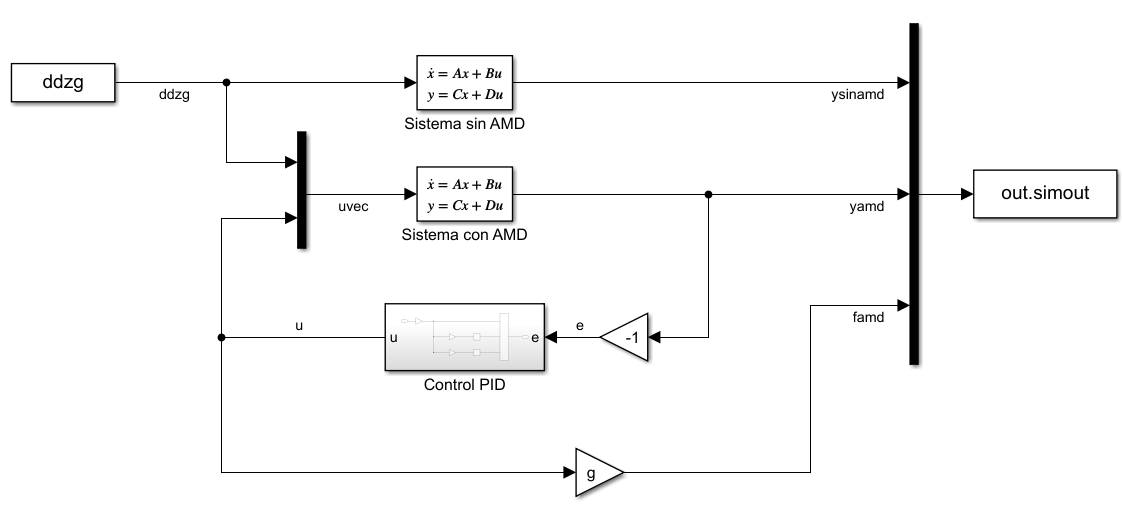
\includegraphics[scale=0.7]{Figuras/Simulink.png}
\end{figure}

\section{Root Locus}
$\Longrightarrow$ ``Migración de polos'', Locus = posición en latín
\begin{align*}
    \text{Planta: }~ G_{y\ddot{z}_g}(s)&=\frac{1/m}{s^2+2\zeta\omega_n s+\omega_n^2}\\
    G_{yu}(s) &=\frac{g/m}{s^2+2\zeta\omega_n s+\omega_n^2}
\end{align*}
\begin{align*}
    \text{Controlador PID: }~C(s)=K_p(1+\frac{T_I}{s}+T_Ds)
\end{align*}

\begin{figure}[H]
\centering
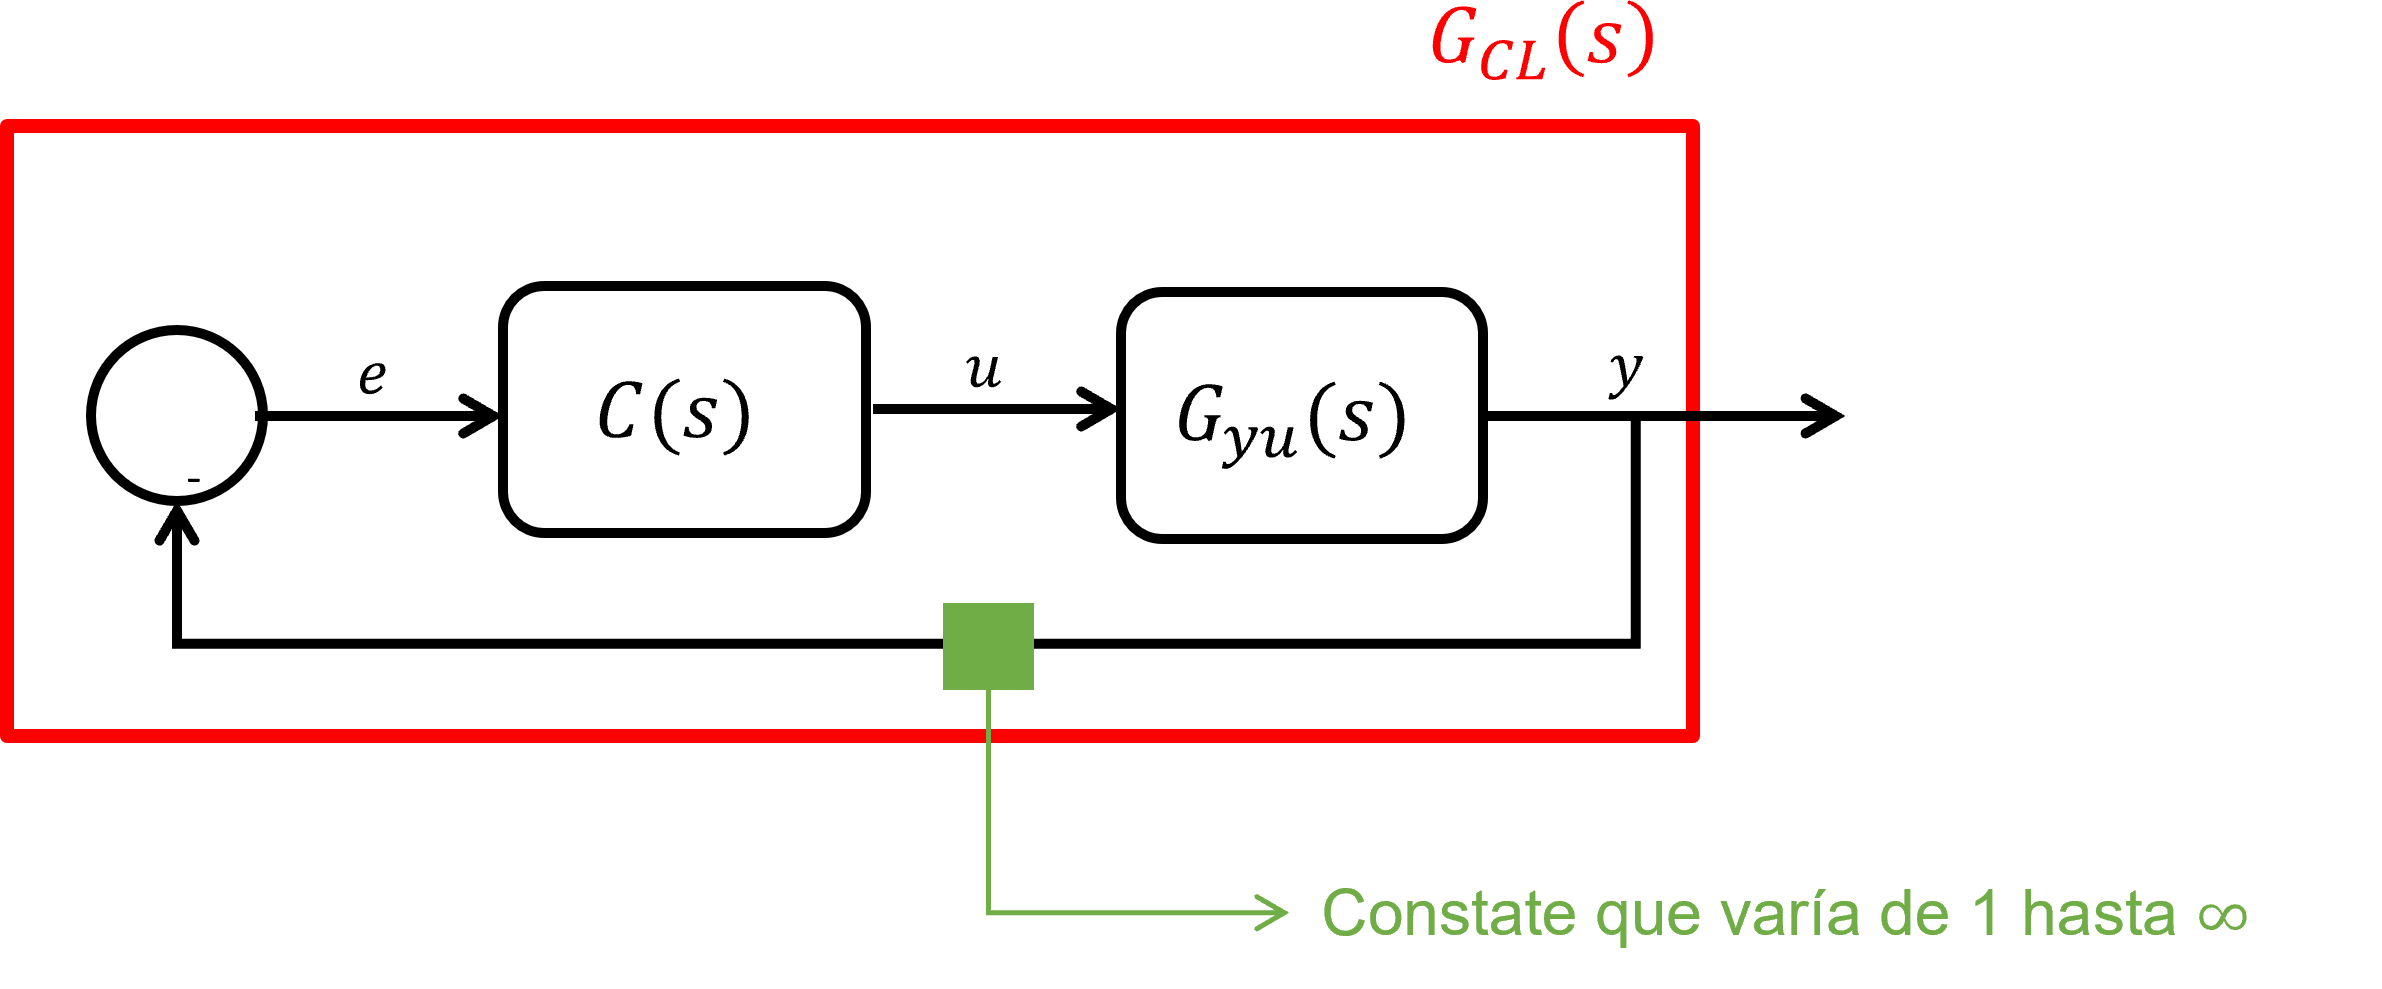
\includegraphics[scale=0.7]{Figuras/GCL.png}
\end{figure}

\begin{align*}
    G_{CL}(s)&=\frac{G(s)C(s)}{1+G(s)C(s)}\\
    G_{CL}(s)&=\frac{G(s)K_p\bigg(1+T_I/s+T_Ds\bigg)}{1+G(s)K_p\bigg(1+T_I/s+T_Ds\bigg)}
\end{align*}

\underline{Resumen control PID}: 
\begin{figure}[H]
\centering
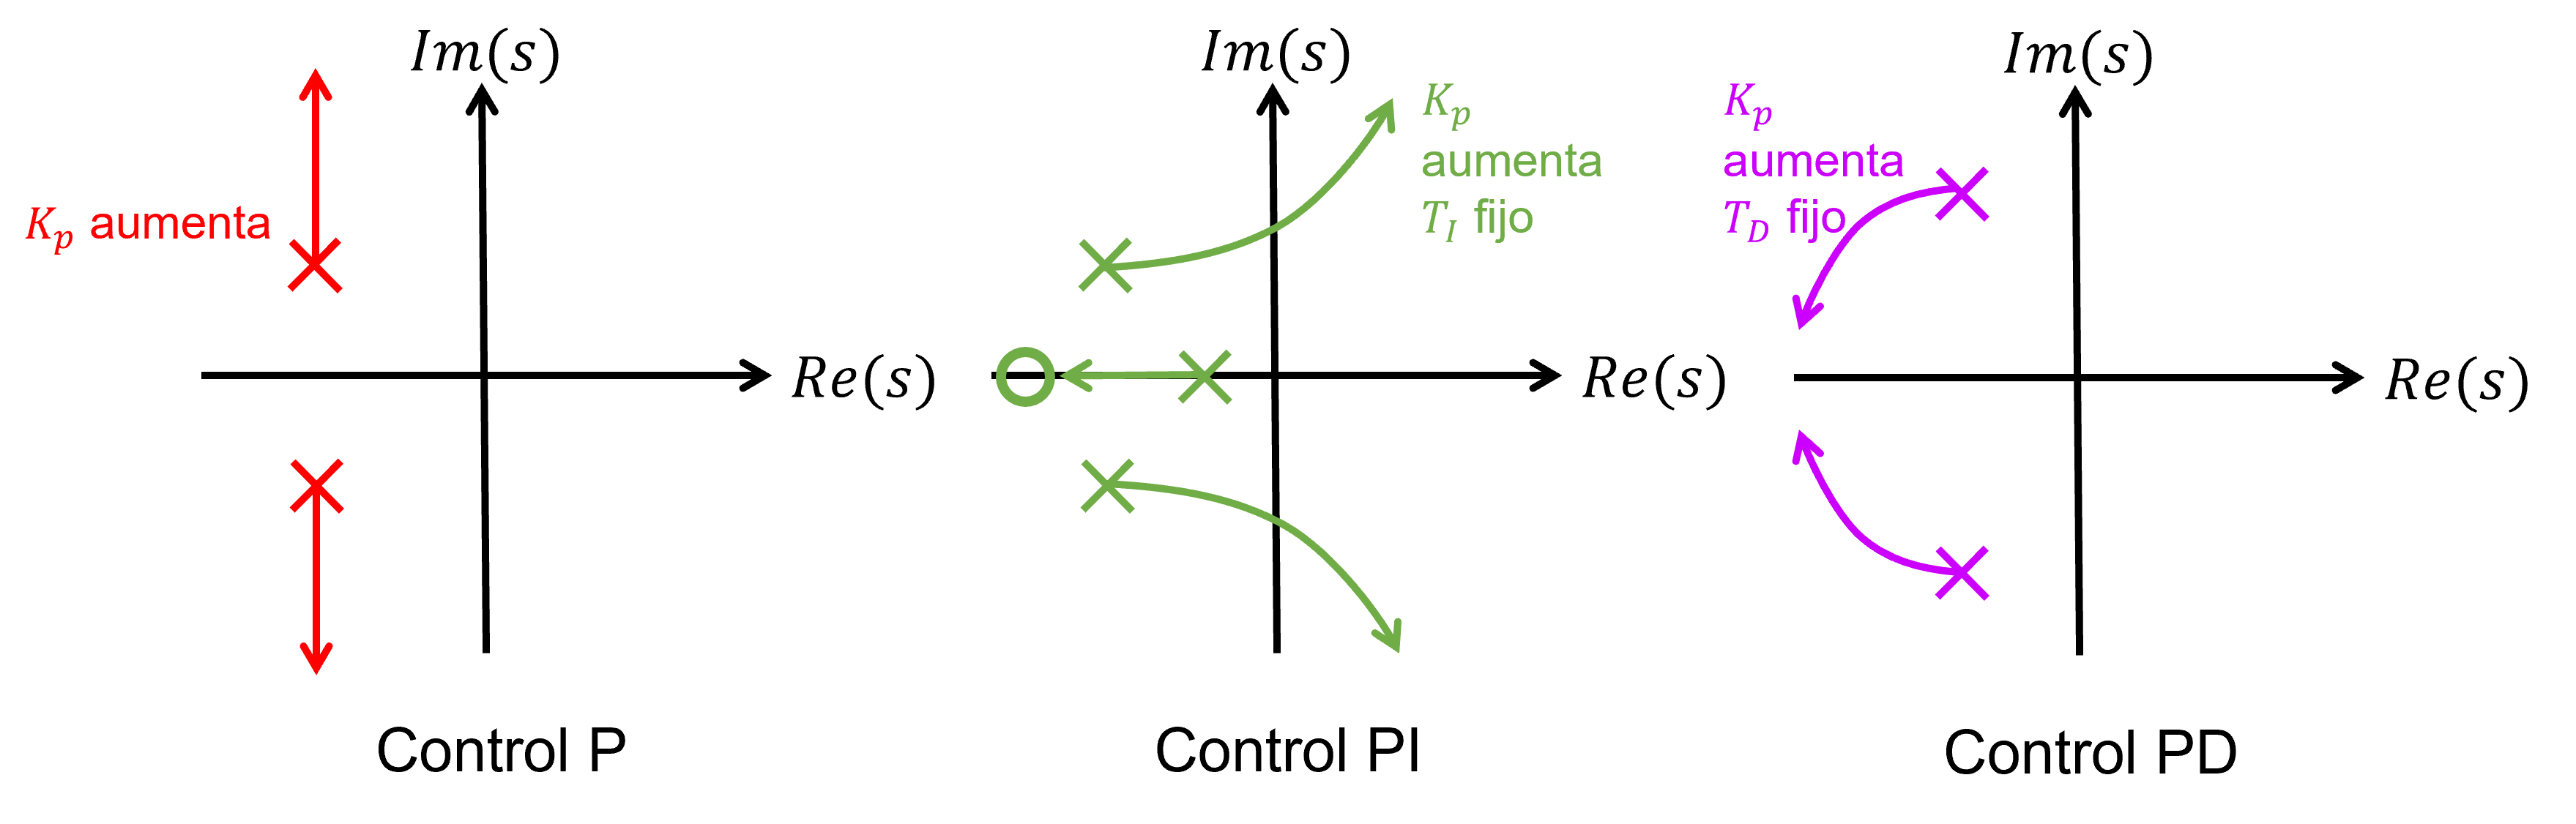
\includegraphics[scale=0.65]{Figuras/controlPID.png}
\end{figure}

\section{Control Moderno}
Representación espacio estado, sistema LTI.\\
\par Sea: 
\begin{align*}
    {x}&=[x_1,x_2,...,x_N]^\top\\
    {u}&=[u_1,u_2,...,u_p]^\top\\
    {y}&=[y_1,y_2,...,y_r]^\top
\end{align*}
\begin{itemize}
    \item[(1)] Ecuación de estado:
    $${\dot{x}}={A}{x}+{B}{u} $$
    \item[(2)] Ecuación de respuesta:
    $${y}={C}{x}+{D}{u} $$
\end{itemize}

\underline{Paréntesis}:
Aplicando la Transformada de Laplace a las ecuaciones de estado y respuesta de la representación espacio-estado:
\begin{align*}
    {\dot{x}}={A}{x}+{B}{u}\xrightarrow[]{\mathcal{L}}s{X}(s)={A}{X}(s)+{B}{U}(s)\\
    \Longrightarrow {X}(s)=(s{I}-{A})^{-1}{B}{U}(s)\\
    G_{xu}(s)=(s{I}-{A})^{-1}{B}
\end{align*}
\begin{align*}
    {y}={C}{x}+{D}{u}\xrightarrow[]{\mathcal{L}}s{Y}(s)={C}{X}(s)+{D}{U}(s)\\
    {Y}(s)=[{C}(s{I}-{A})^{-1}{B}+{D}]{U}(s)\\
    G_{yu}={C}(s{I}-{A})^{-1}{B}+{D}
\end{align*}


\section{Formas canónicas}
\subsection{Forma Canónica Controlable (CCF)}
Asumir que ${D}={0}$ (no hay componente ``feedthrough'' en la salida del sistema).
\begin{align*}
{A_c}=\left[
    \begin{array}{cccc|c}
     -a_1 & -a_2 & \dots & -a_{n-1} & -a_n\\ \hline
     1 & & & 0 & 0\\
       & 1 & & & \vdots\\
       & & \ddots & & \\
     0 & & & 1 & 0  
    \end{array}\right], \quad {A_c}\in \mathbb{R}^{n\times n}
\end{align*}
\begin{align*}
{B_c}=\left[
    \begin{array}{c}
     1 \\ \hline
     0\\
    \vdots\\
     0  
    \end{array}\right], \quad {B_c}\in \mathbb{R}^{n\times 1}
\end{align*}
\begin{align*}
{C_c}=\left[
    \begin{array}{cccc}
     b_1 & b_2 & \dots & b_n
    \end{array}\right], \quad {C_c}\in \mathbb{R}^{1\times n}
\end{align*}
\begin{align*}
    \text{Realización (SISO): }\quad 
    \left\{
    \begin{array}{l}
          {\dot{x}_c}={A_c}{x_c}+{B_c}u \\
          y={C_c}{x_c} \\
    \end{array} 
    \right. 
\end{align*}
Notar que:
\begin{align*}
    \dot{x}_1 &= -a_1x_1-a_2x_2 ... -a_nx_n+1\cdot u\\
    \dot{x}_2 &= x_1\\
    \dot{x}_3 &= x_2\\
    \vdots \\
    \dot{x}_n &= x_{n-1}
\end{align*}

Utilizando la transformada de Laplace, se obtiene la siguiente función de transferencia:
\begin{align*}
    G_{yu}(s)=\frac{b_1s^{n-1}+b_2s^{n-2}+...+b-n}{s^n+a_1s^{n-1}+a_2s^{n-2}+...+a_n} = \frac{\text{numerador orden n-1}}{\text{denominador orden n}} = \text{TF Propia}
\end{align*}

Se utiliza para diseñar controladores cuando todos los estados del sistema son conocidos.

\subsection{Forma Canónica Modal (MCF)}
Sea $G(s)=\frac{c_1}{s+p_1}+\frac{c_2}{s+p_2}+...+\frac{c_n}{s+p_n}$, $G(s)$ se escribe como una expansión de fracción parcial, y los polos $p_i$ son todos distintos:
\begin{align*}
{A_m}=\left[
    \begin{array}{cccc}
     -p_1& & & 0\\
     & -p_2 & & \\
     & & \ddots & \\
     0 & & & -p_n
    \end{array}\right], \quad {A_m}\in \mathbb{R}^{n\times n}
\end{align*}
\begin{align*}
{B_m}=\left[
    \begin{array}{c}
     1 \\ 
     1\\
    \vdots\\
     1  
    \end{array}\right], \quad {B_m}\in \mathbb{R}^{n\times 1}
\end{align*}
\begin{align*}
{C_m}=\left[
    \begin{array}{cccc}
     c_1 & c_2 & \dots & c_n
    \end{array}\right], \quad {C_m}\in \mathbb{R}^{1\times n}
\end{align*}

\begin{align*}
    \text{Realización (SISO): }\quad 
    \left\{
    \begin{array}{l}
          {\dot{x}_m}={A_m}{x_m}+{B_m}\cancelto{0}{u} 
    \end{array} 
    \right. 
\end{align*}

\begin{align*}
    \dot{x}_{m_1} &= \lambda_1x_{m_1}\\
    \dot{x}_{m_2} &= \lambda_2x_{m_1}\\
    \vdots \\
    \dot{x}_{m_n} &= \lambda_nx_{m_n}
\end{align*}

\begin{align*}
    \Longrightarrow{\dot{x}}={A}{x}
\end{align*}

\underline{Resolver}: ${A}{v}=\lambda {v}$ (Problema de valores propios de ${A}$).\\
\par ${T}$ es la matriz de transformación modal, ${T}=[{v_1},{v_2},...,{v_n}]$\\

\subsection{Forma Canónica Observable (OCF)}
Dado $G(s)=\frac{n(s)}{d(s)}$, con $a_i$, $b_i$ conocidos.

\begin{align*}
{A_o}=\left[
    \begin{array}{c|cccc}
     -a_{n-1} & 1 & & & 0 \\ 
     -a_{n-2} & & 1 & & \\
     \vdots   & & & \ddots & \\
     -a_1     & 0 & & & 1 \\ \hline
     -a_0     & 0 & 0 & \dots & 0   
    \end{array}\right], \quad {A_o}\in \mathbb{R}^{n\times n}
\end{align*}
\begin{align*}
{B_o}=\left[
    \begin{array}{c}
     b_{n-1} \\
     b_{n-2}\\
    \vdots\\
     b_1 \\ \hline
     b_0
    \end{array}\right], \quad {B_o}\in \mathbb{R}^{n\times 1}
\end{align*}
\begin{align*}
{C_o}=\left[
    \begin{array}{c|ccc}
     1 & 0 & \dots & 0
    \end{array}\right], \quad {C}_o\in \mathbb{R}^{1\times n}
\end{align*}

Se utiliza para diseñar ``observadores''.


\section{Control lazo cerrado utilizando estados (State Feedback Control)}

\begin{figure}[H]
\centering
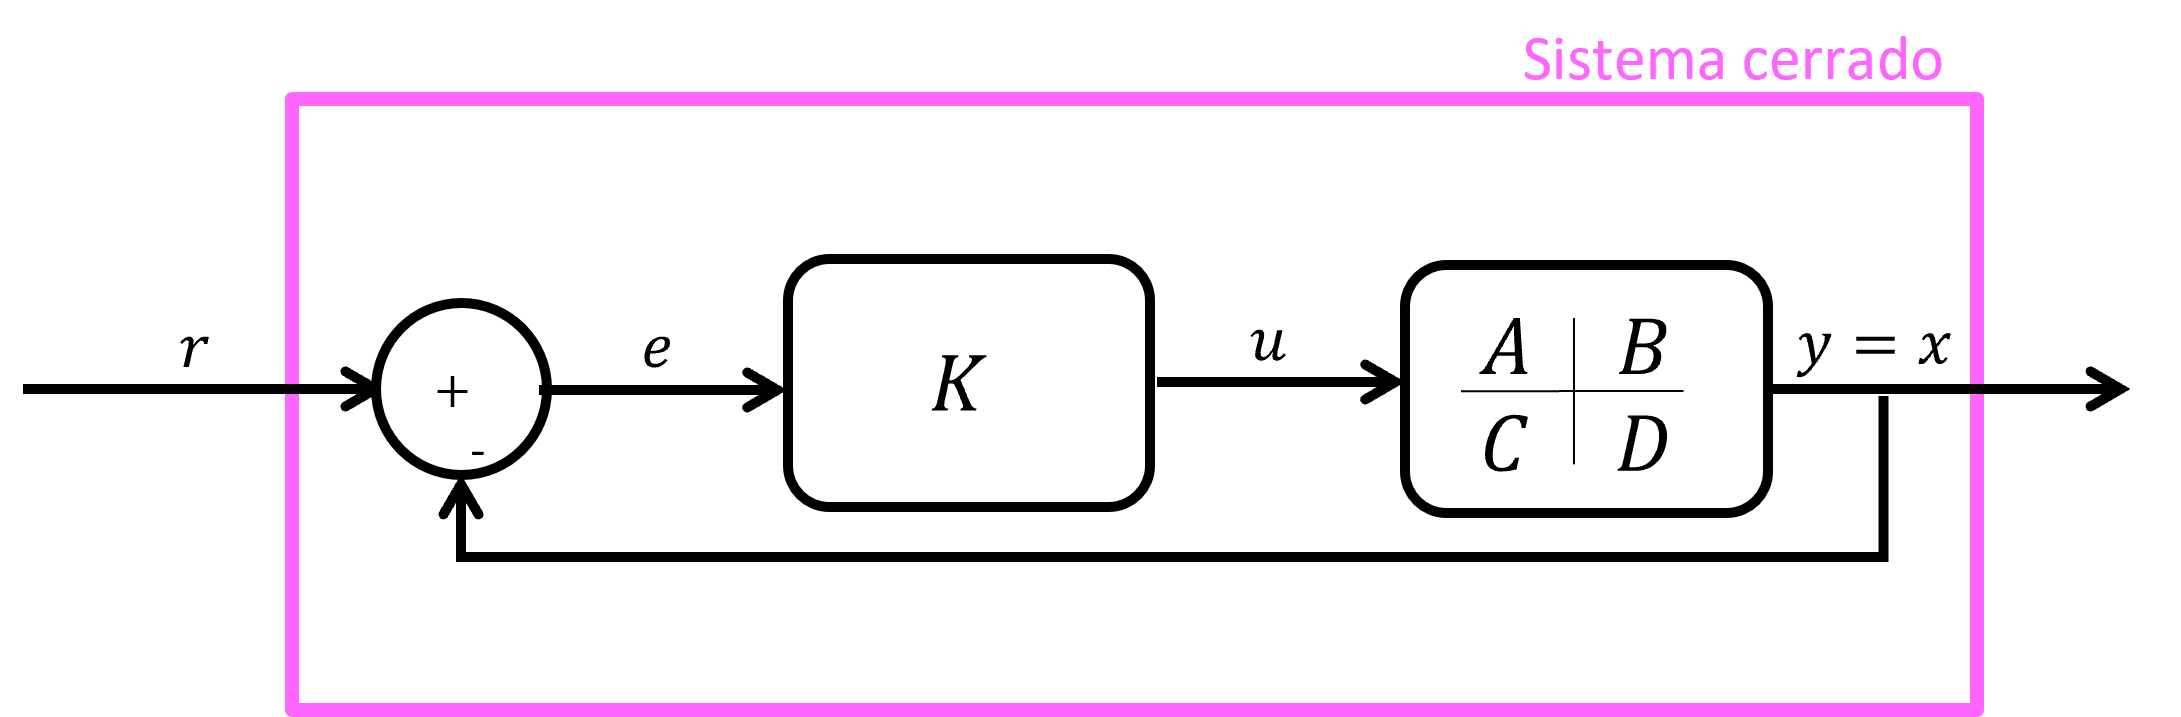
\includegraphics[scale=0.7]{Figuras/State_feedback.png}
\end{figure}
\underline{Objetivo}: Diseñar $K$ tal que $e=r-x\to 0$ para un tiempo $t_f$.\\
\par \underline{Definición}: El sistema de control ``full state feedback'' tiene relación con el hecho que el controlador cuenta con acceso a todos los estados del sistema.\\

\par Veamos la ecuación de estado del sistema:
\begin{align*}
    \dot{x}=Ax+Bu
\end{align*}
La señal de control:
\begin{align*}
    u=Ke
\end{align*}
La señal de error:
\begin{align*}
    e=r-x
\end{align*}

Luego:

\begin{align*}
    \dot{x} &= Ax+BK(r-x)\\
    \dot{x} &= (A-BK)x+BKr\\
\end{align*}

\begin{itemize}
    \item $A_{CL}=A-BK$: matriz de estado del sistema cerrado.
    \item $B_{CL}=BK$
\end{itemize}

\begin{align*}
    \dot{x}=A_{CL}x+B_{CL}r
\end{align*}

Para que el sistema cerrado sea \textcolor{red}{ESTABLE}, los valores propios de $A_{CL}$ deben tener partes reales estrictamente negativas:

\begin{align*}
    \Re(\text{eig}(A_{CL}))<0
\end{align*}

\par Analicemos el diseño de un controlador utilizando una representación CCF:

\begin{align*}
{A}=\left[
    \begin{array}{cccc|c}
     -a_1 & -a_2 & \dots & -a_{n-1} & -a_n\\ \hline
     1 & & & 0 & 0\\
       & 1 & & & \vdots\\
       & & \ddots & & \\
     0 & & & 1 & 0  
    \end{array}\right]_{n\times n}
\end{align*}
\begin{align*}
{B}=\left[
    \begin{array}{c}
     1 \\ \hline
     0\\
    \vdots\\
     0  
    \end{array}\right]_{n\times 1}
\end{align*}
\begin{align*}
{K}=\left[
    \begin{array}{ccccc}
     k_{n-1} & k_{n-2} & \dots & k_1 & k_0
    \end{array}\right]_{1\times n}
\end{align*}

Calculemos $BK$:
\begin{align*}
{BK}=\left[
    \begin{array}{cccc|c}
     k_{n-1} & k_{n-2} & \dots & k_1 & k_0\\ \hline
      & & & & 0\\
      & & {0}_{(n-1)\times(n-1)} & & \vdots\\
      & & & & 0  
    \end{array}\right]_{n\times n}
\end{align*}

Ahora, calculemos $A_{CL}=A-BK$
\begin{align*}
{BK}=\left[
    \begin{array}{cccc|c}
     -(a_{n-1}+k_{n-1}) & -(a_{n-2}+k_{n-2}) & \dots & -(a_1+k_1) & -(a_0+k_0)\\ \hline
      & & & & 0\\
      & & {I}_{(n-1)\times(n-1)} & & \vdots\\
      & & & & 0  
    \end{array}\right]_{n\times n}
\end{align*}

Queremos encontrar los valores propios de $A_{CL}$. Escribamos la ecuación característica de $A_{CL}$
\begin{align*}
    \det({A_{CL}}-\lambda {I})=0
\end{align*}

\begin{align*}
{BK}=\left[
    \begin{array}{cccc|c}
     -(\lambda+a_{n-1}+k_{n-1}) & -(a_{n-2}+k_{n-2}) & \dots & -(a_1+k_1) & -(a_0+k_0)\\ \hline
      1 & -\lambda & & & 0\\
      & 1 & -\lambda & & \vdots\\
      & & \ddots & \ddots & 0\\
      & & & 1 & -\lambda\\
    \end{array}\right]=0
\end{align*}

La ecuación característica resulta ser:
\begin{align*}
    \lambda^n+(a_{n-1}+k_{n-1})\lambda^{n-1}+(a_{n-2}+k_{n-2})\lambda^{n-2}+...+(a_{1}+k_{1})\lambda+(a_{0}+k_{0})=0
\end{align*}
Si queremos ubicar los polos en una posición particular, o sea, queremos fijar los polos de la siguiente manera:
$$ \lambda=\{p_1,p_2,p_3,..,p_n \}$$

Podemos reescribir la ecuación característica de la siguiente forma:
$$(\lambda-p_1)(\lambda-p_2)(\lambda-p_3)...(\lambda-p_n)=0 $$

Desarrollando el polinomio:
$$\Longrightarrow \lambda^n+\alpha_{n-1}\lambda^{n-1}+...+\alpha_1\lambda+\alpha_0=0 $$
Entonces, el controlador $K$ se define como:
\begin{align*}
    \alpha_{n-1} = a_{n-1}+k_{n-1} &\Longrightarrow k_{n-1} = \alpha_{n-1}-a_{n-1}\\
    \alpha_{n-2} = a_{n-2}+k_{n-2} &\Longrightarrow k_{n-2} = \alpha_{n-2}-a_{n-2}\\
    \vdots \\
    \alpha_0 = a_0+k_0 &\Longrightarrow k_0 = \alpha_0-a_0\\
\end{align*}

Donde $\alpha_i$ se obtiene de la posición deseada de los polos. \\

\par Entonces, si el sistema es CCF, podemos diseñar $K$ al elegir la posición de los polos de manera apropiada $\Longrightarrow$ \textbf{POLE PLACEMENT}\\

\par \underline{Nota}: Si el sistema no es CCF, entonces se puede transformar a CCF utilizando matriz de transformación ${T}$, provisto que el sistema sea controlable.\\

\par Sea la realización:

\begin{align*}
    {x}=Ax+Bu \xrightarrow[]{x=Tz} \dot{z}=A_cz+B_cu
\end{align*}
Sea $T \in \mathbb{R}^{n\times n}$, tal que $T^{-1}$ existe
\begin{align*}
    \Longrightarrow x&=Tz\\
    \Longrightarrow \dot{x}&=T\dot{z}
\end{align*}
Reemplazando:
\begin{align*}
    T\dot{z} &= ATz+Bu\\
    \Longrightarrow \dot{z}&=T^{-1}ATz+T^{-1}Bu\\
    \dot{z} &= A_cz+B_cu
\end{align*}

``Pole placement'', pasos a seguir:
\begin{enumerate}
    \item Buscar $T$ y transformar a CCF ($A_c$ y $B_c$).
    \item Encontrar $K_c$ , en base a la ubicación de polos deseados.
    \item Volver al sistema original (asuma $r=0$)
\end{enumerate}
\begin{align*}
    \Longrightarrow \dot{z} &= (A_c-B_cK_c)z\\
    \Longrightarrow T\dot{z} &= TA_cz+TB_cz\\
    \Longrightarrow \dot{x} &= TT^{-1}ATz-TT^{-1}BK_cz\\
    \Longrightarrow \dot{x} &= Ax-BK_cT^{-1}x\\
    \Longrightarrow \dot{x} &= (A-BK)x
\end{align*}
donde  $K=K_cT^{-1}$, controlador para el sistema original.

\section{Observadores}
\underline{Motivación}: \\

Considere el siguiente ejemplo de sistema dinámico:
\begin{align*}
    \dot{x} &= f(x,u)\\
    y &= g(x,u)
\end{align*}

\begin{figure}[H]
\centering
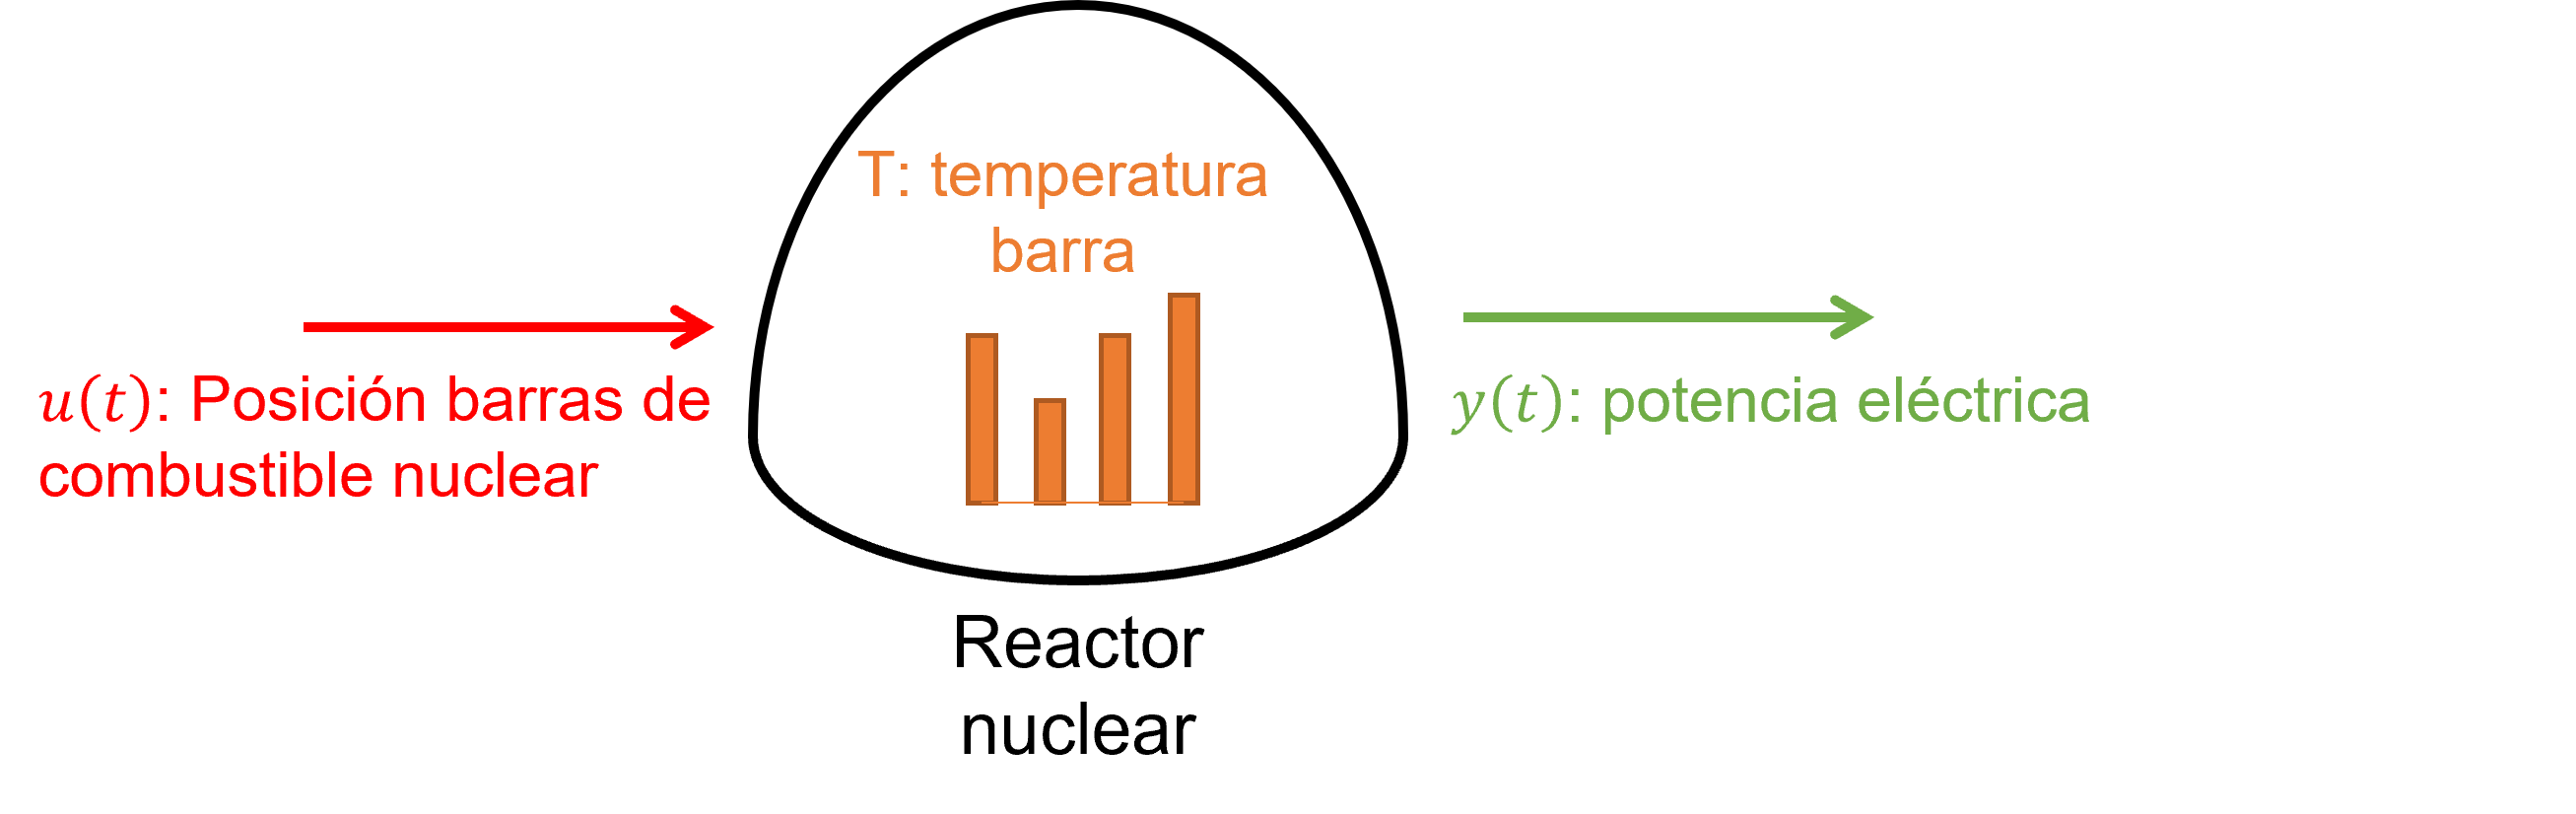
\includegraphics[scale=0.7]{Figuras/nuclear.png}
\end{figure}
¿Es posible determinar los estados internos del sistema $x(t)$ (temperatura de las barras), utilizando solo las señales de entrada y salida $\{u(t), y(t)\}$? La respuesta es sí, pero con la condición de que el sistema sea \textbf{observable}.\\

El objetivo de lo que se desarrollará a continuación es \emph{diseñar} un \emph{observador/estimador} para poder estimar los estados internos $x(t)$ de un sistema, de tal forma que dependa únicamente de las señales de entrada y salida del sistema:

\begin{align*}
    \hat{x}(t) = f(u(t), y(t))
\end{align*}

\begin{figure}[H]
\centering
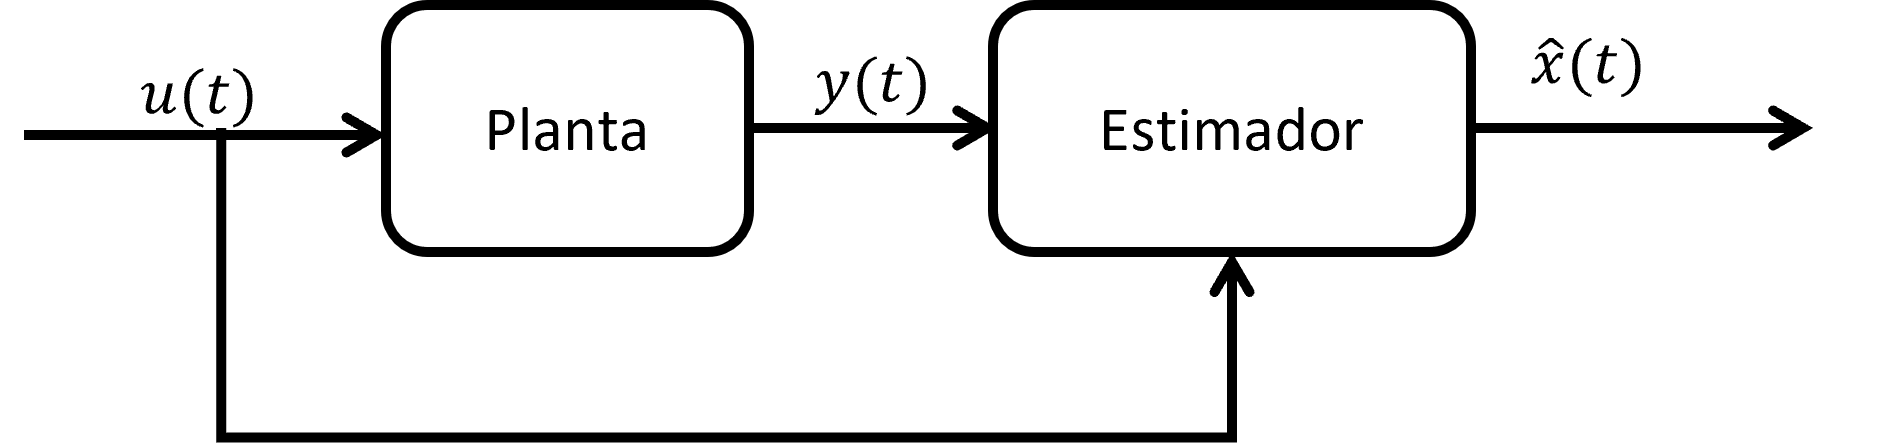
\includegraphics[scale=0.7]{Figuras/observador2.png}
\end{figure}

\underline{Notación}:
\begin{itemize}
    \item $x(t)$: estados del sistema
    \item $\hat{x}(t)$: estados estimados
    \item $\tilde{x}(t)=x(t)-\hat{x}(t)$: error de estimación
\end{itemize}

La dinámica del sistema de los \emph{estados estimados} $\hat{x}$ es la misma que la del sistema planta:

\begin{align*}
    &\dot{\hat{x}} = A\hat{x}+Bu \\
    &\hat{x}(0) = \hat{x}_0    
\end{align*}

Luego, se puede deducir la dinámica del \emph{error de estimación} $\tilde{x}$:

\begin{align*}
    \dot{\tilde{x}} &= \frac{d}{dt}(x-\hat{x})=\dot{x}-\dot{\hat{x}}\\
    &= (Ax+Bu)-(A\hat{x}+Bu)=A(x-\hat{x}) \\
    \Longrightarrow \dot{\tilde{x}} &= A\tilde{x} 
\end{align*}

La estrategia para diseñar el observador es la siguiente: Si los estados decaen a cero, entonces se diseña un estimador tal que el error de la estimación decae con la misma tasa que el sistema.

\begin{figure}[H]
\centering
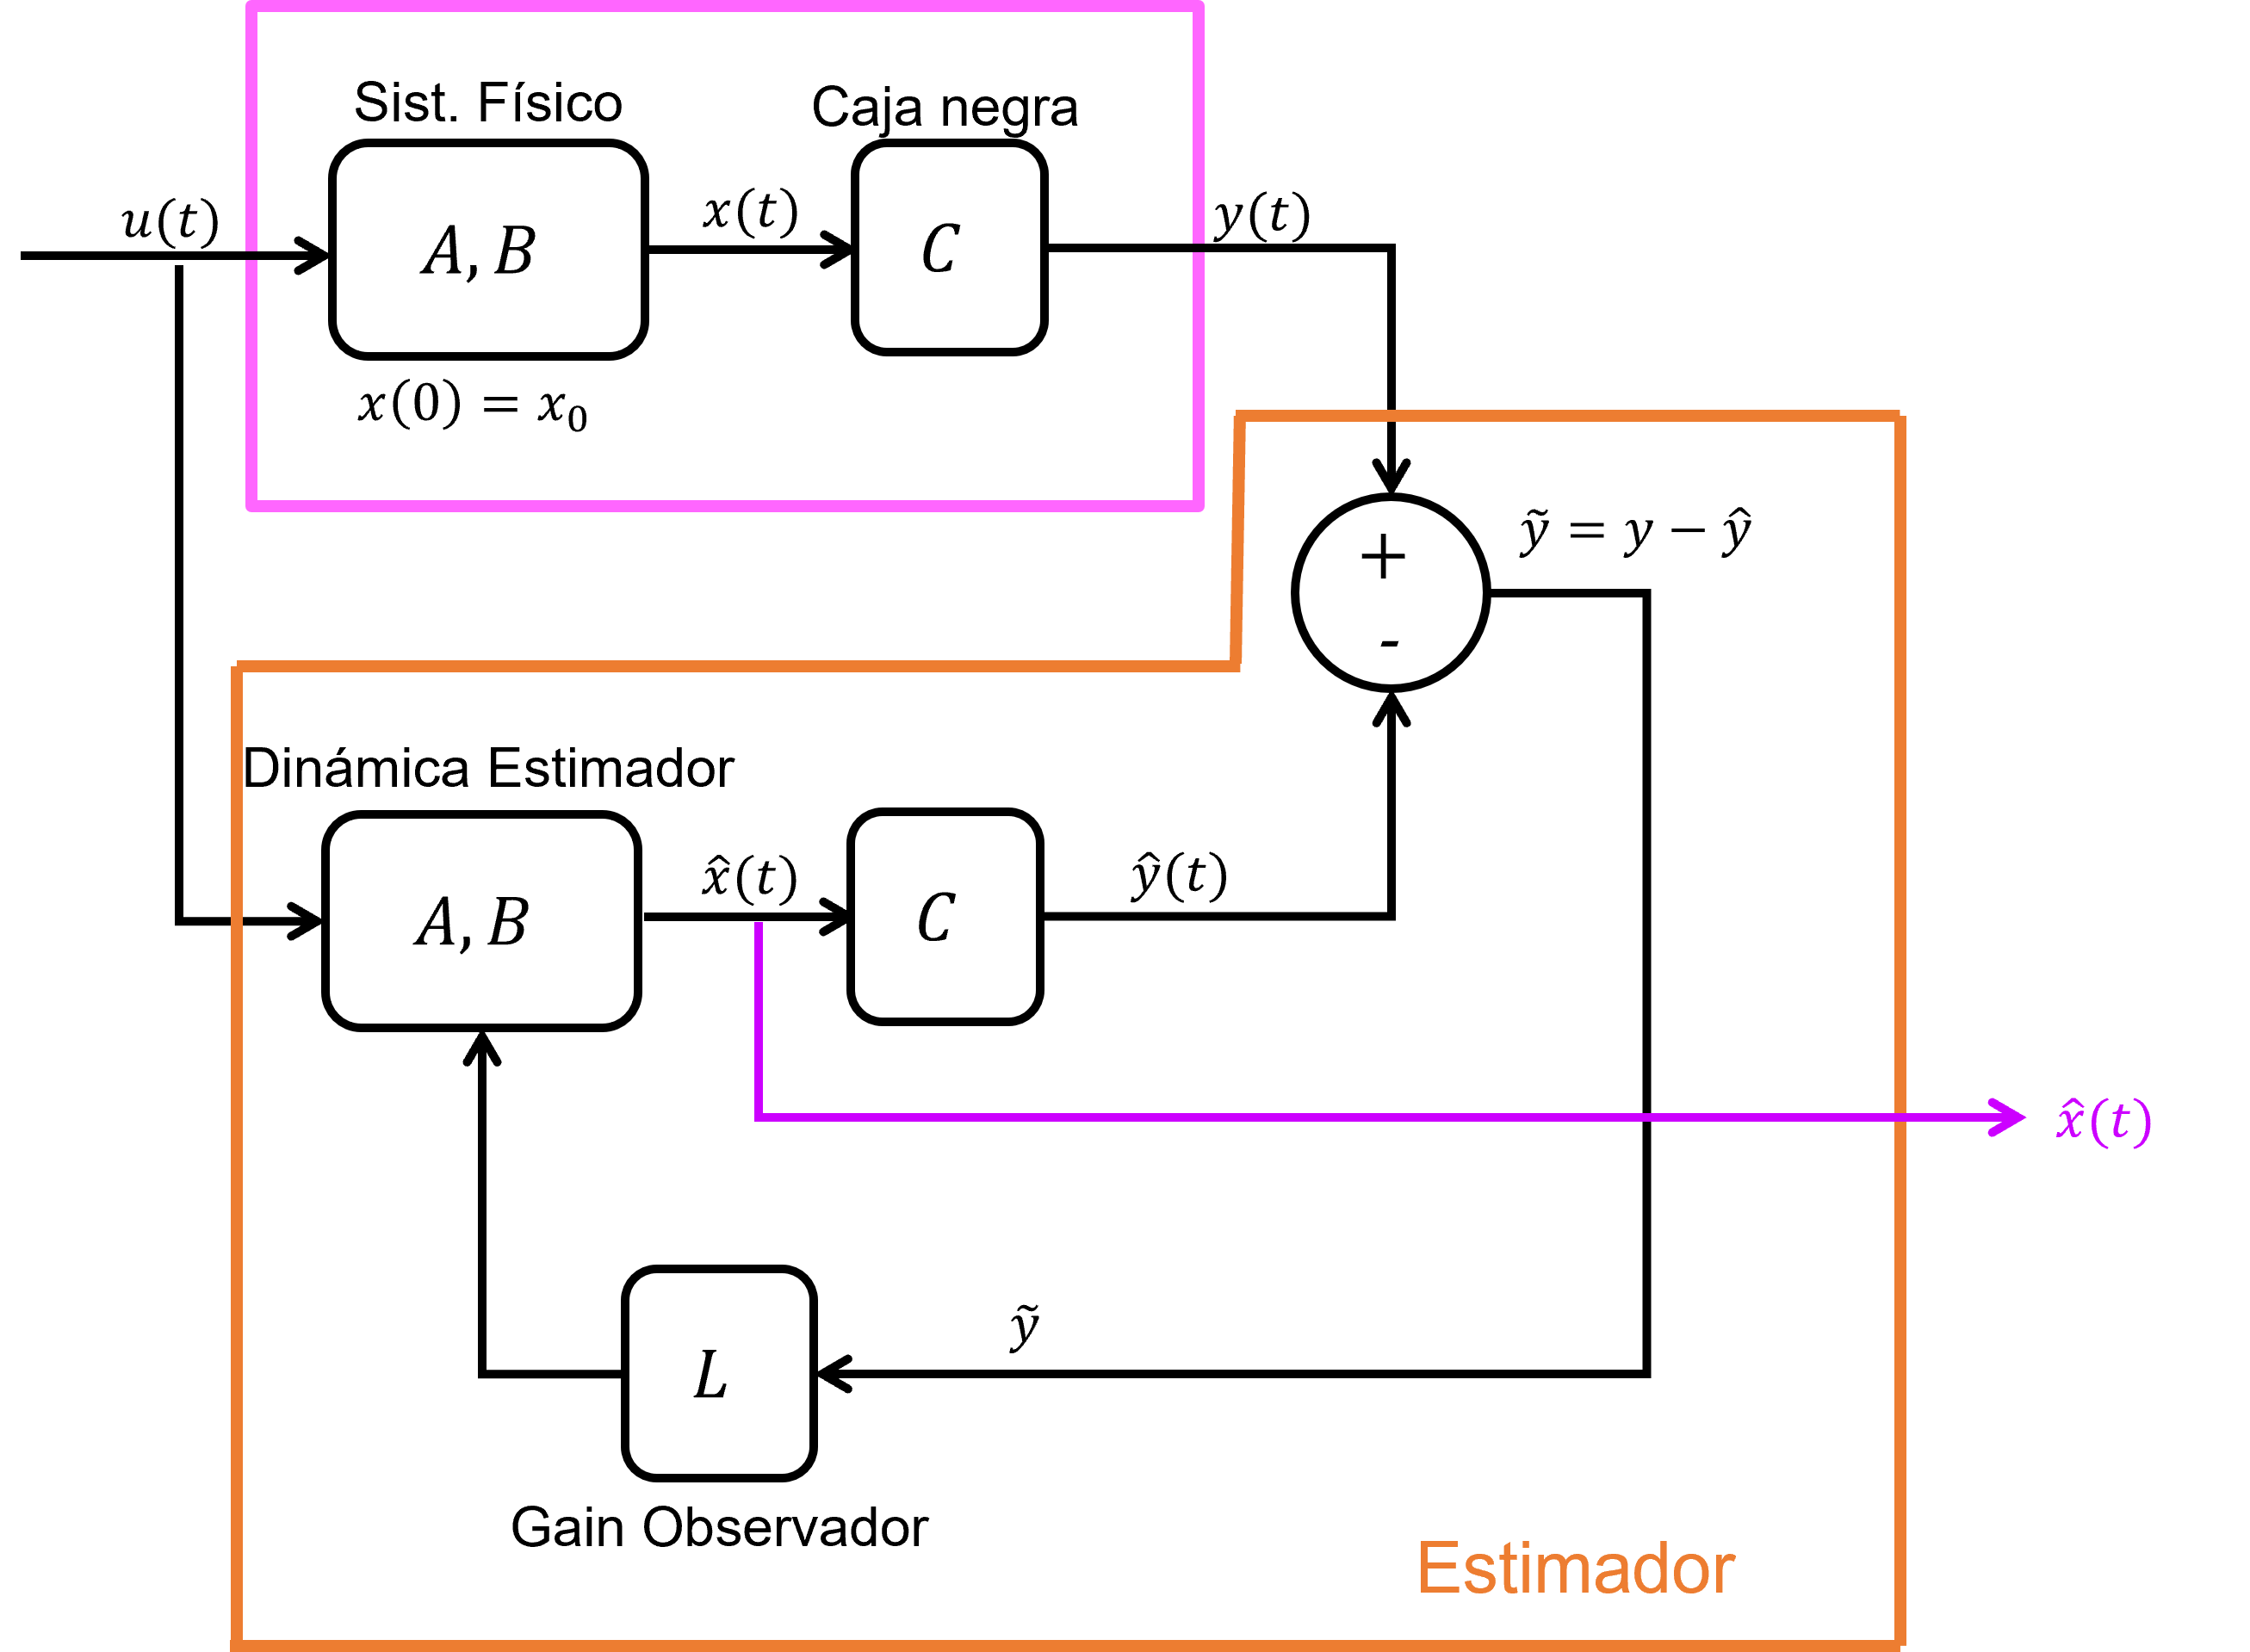
\includegraphics[scale=0.8]{Figuras/observador.png}
\end{figure}

\section{Diseño de Observador de Estados}
De la figura anterior, notar que para estimar los estados del sistema, se requiere de una ganancia $L$. Lo que se va a realizar a continuación es diseñar esta matriz $L$. \\

La representación espacio-estado de los estados estimados $\hat{x}(t)$ incluye la señal del error de estimación $\tilde{x}$ y su ganancia $L$.

\begin{align*}
    \dot{\hat{x}}(t) = A\hat{x}(t)+Bu(t)+L\tilde{y}(t)
\end{align*}
donde:
\begin{align*}
    L=\left[
    \begin{array}{c}
     l_1 \\ l_2\\ \vdots\\ l_n 
    \end{array}\right], \quad L \in \mathbb{R}^{n\times r}, \quad x,y \in \mathbb{R}^n 
\end{align*}

La ecuación de estado del error de estimación queda de la siguiente forma:
\begin{align*}
    \dot{\tilde{x}}=\dot{x}-\dot{\hat{x}} &= (Ax+Bu)-(A\hat{x}+Bu+L\tilde{y})\\
    &= A\tilde{x}-L(y-\hat{y})\\
    &= A\tilde{x}-L(Cx-C\hat{x})\\
    &= A\tilde{x}-LC\tilde{x}\\
    \dot{\tilde{x}} &= (A-LC)\tilde{x}
\end{align*}

Por lo tanto, para diseñar $L$, $(A-LC)$ debe cumplir con estabilidad. Para lograr esta estabilidad, se ubicarán apropiadamente los polos de forma que se encuentren al lado izquierdo del plano complejo. A esta estrategia se le conoce como \textbf{Pole Placement}. \\

\underline{Caso particular}: 

Considere el siguiente sistema con $x\in\mathbb{R}^n$, $u\in\mathbb{R}$, $y\in\mathbb{R}$: 

\begin{align*}
    G(s) = \frac{b_0}{s^n+a_{n-1}s^{n-1}+...+a_1s+a_0}
\end{align*}

Su Forma Canónica Observable es: 

\begin{align*}
{A_o}=\left[
    \begin{array}{c|cccc}
     -a_{n-1} & 1 & & & 0 \\ 
     -a_{n-2} & & 1 & & \\
     \vdots   & & & \ddots & \\
     -a_1     & 0 & & & 1 \\ \hline
     -a_0     & 0 & 0 & \dots & 0   
    \end{array}\right], \quad {A_o}\in \mathbb{R}^{n\times n}
\end{align*}
\begin{align*}
{B_o}=\left[
    \begin{array}{c}
     b_{n-1} \\
     b_{n-2}\\
    \vdots\\
     b_1 \\ \hline
     b_0
    \end{array}\right], \quad {B_o}\in \mathbb{R}^{n\times 1}
\end{align*}
\begin{align*}
{C_o}=\left[
    \begin{array}{c|ccc}
     1 & 0 & \dots & 0
    \end{array}\right], \quad {C}_o\in \mathbb{R}^{1\times n}
\end{align*}

Como en este caso particular, $y\in\mathbb{R}$, entonces $L$ es matriz $n \times 1$:
\begin{align*}
    L=\left[
    \begin{array}{c}
     l_{n-1} \\ l_{n-2}\\ \vdots\\ l_0 
    \end{array}\right] 
\end{align*}
%\underline{Objetivo}: Determinar los $l_i$, $i\in[0,n-1]$

Por lo tanto, se puede obtener $A_0 - LC_0$ de la siguiente forma:
\begin{align*}
    LC_o&=\left[
    \begin{array}{c}
     l_{n-1} \\ l_{n-2}\\ \vdots\\ l_0 
    \end{array}\right] \left[
    \begin{array}{c c c c}
     1 & 0 & ... & 0
    \end{array}\right] =\left[
    \begin{array}{c|c}
     l_{n-1} & \\ \vdots & {0} \\ l_0 & 
    \end{array}\right] \\
    A_o-LC_o &= \left[ \begin{array}{c|c c c}
     -a_{n-1}-l_{n-1} & & & \\  -a_{n-2}-l_{n-2} & & & \\ \vdots & & {I} & \\-a_1-l_1 & & & \\ \hline \\ -a_0-l_0 & 0 & ... & 0
    \end{array}\right] 
\end{align*}
y su ecuación característica es: 
\begin{align*}
    &\phantom{\Longrightarrow} \Delta(A_o-LC_o) = 0 \\
    &\Longrightarrow s^n+(a_{n-1}+l_{n-1})s^{n-1}+...+(a_1+l_1)s+(a_0+l_0) = 0
\end{align*}

Cada coeficiente $(a_i+l_i)$, son los coeficientes $\lambda_i$ del polinomio característico asociado a la ubicación de polos deseada $p_i$:

\begin{align*}
    \prod_{i=0}^{n-1}(s-p_i)=s^n+\lambda_{n-1}s^{n-1}+...+\lambda_1s+\lambda_0=0
\end{align*}

Para finalmente obtener los términos $l_i$ de la matriz $L$, se deben definir los polos deseados, expandir el polinomio y luego igualar ambos términos para todo $i \in [0,n-1]$.

\begin{align*}
    &\phantom{\longrightarrow} a_i + l_i = \lambda_i \\
    &\longrightarrow l_i = a_i-\lambda_i
\end{align*}

\underline{Nota}: En MATLAB, el diseño por ubicación de polos se puede realizar utilizando el comando \texttt{place()}. \\

\underline{Nota}: Si el sistema no está escrito en OCF (forma canónica observable), es recomendable transformarlo a OCF con una transformación de similitud utilizando la matriz $T$. Recordar que esta matriz $T$ existe ssi el sistema es observable.


\section{Principio de Separación}
Considere el siguiente sistema LTI cerrado:
\begin{figure}[H]
\centering
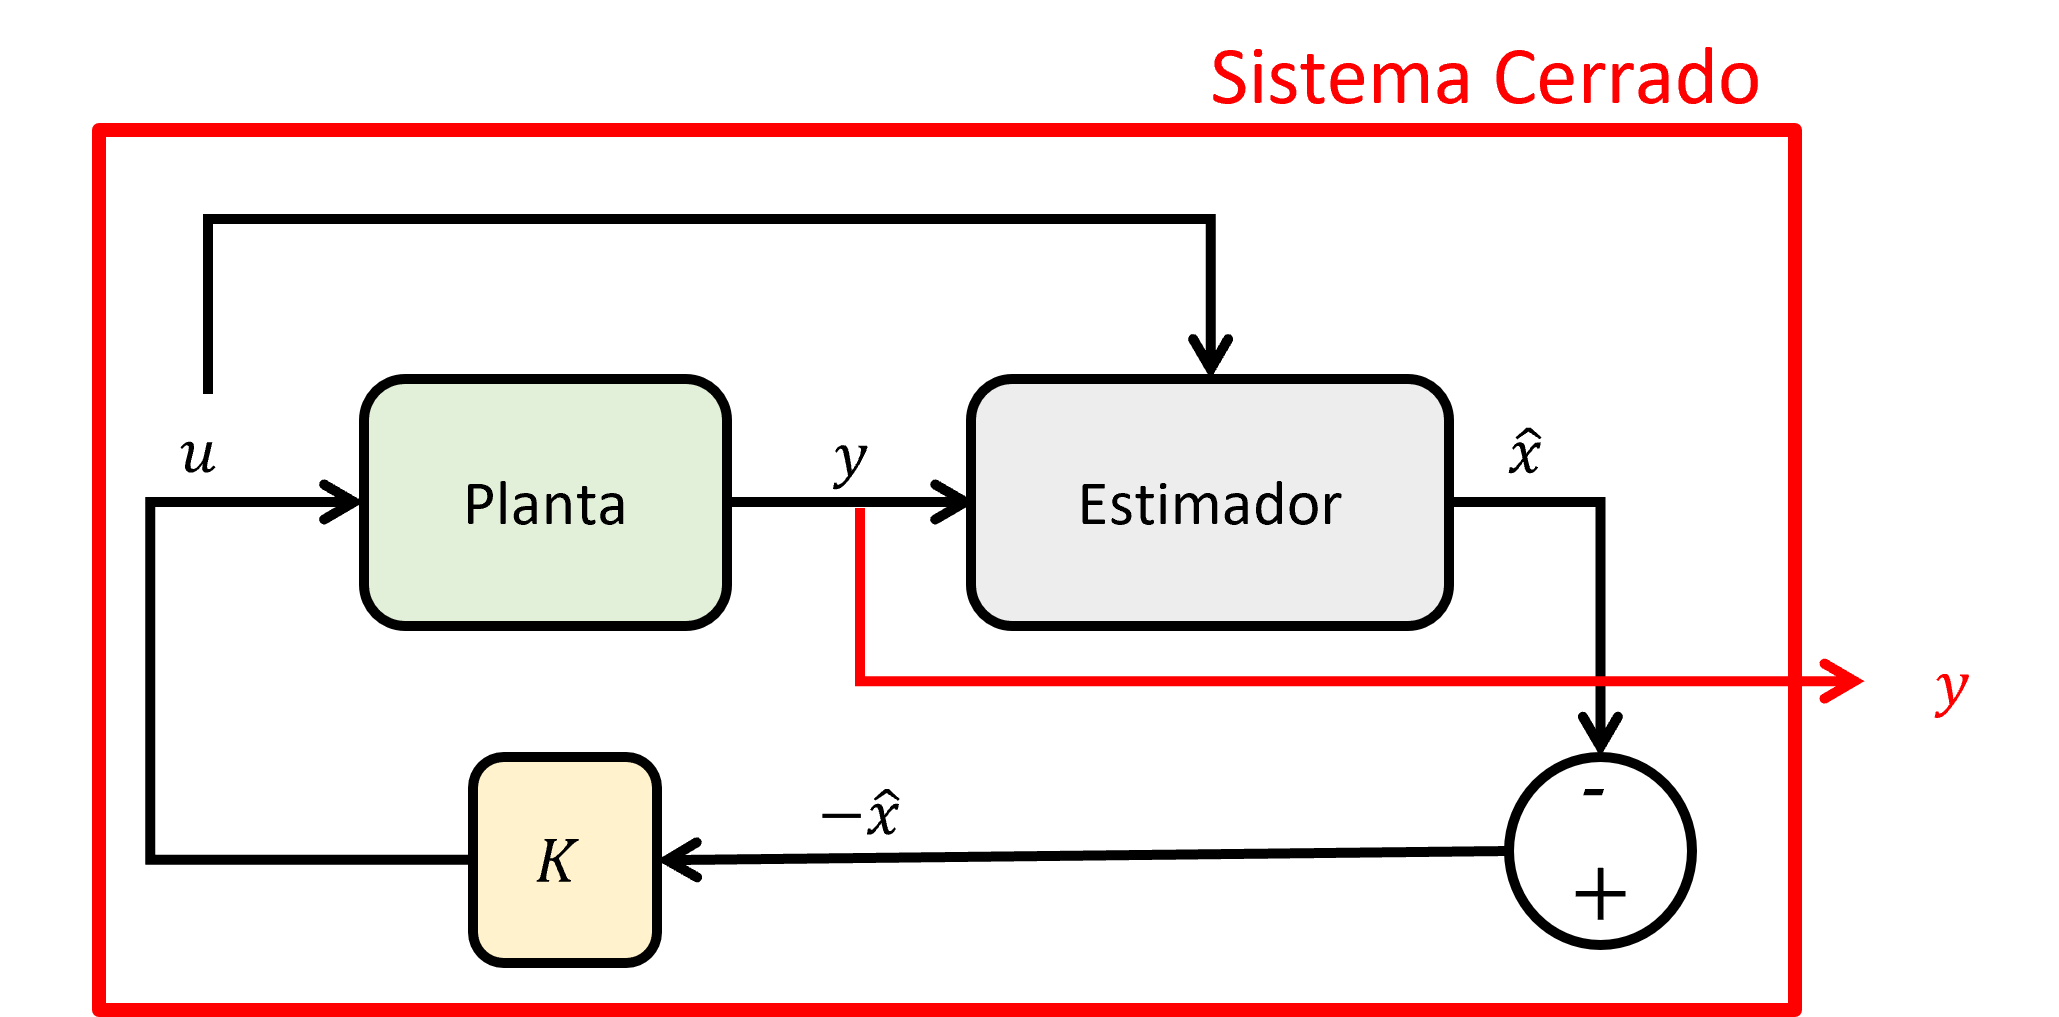
\includegraphics[scale=0.7]{Figuras/ppio_separacion.png}
\end{figure}


Planta:
\begin{subequations}
    \begin{align}
        \dot{x} &= Ax+Bu\\
        y &= Cx
    \end{align}
\end{subequations}

Controlador:
\begin{subequations}
    \begin{align}
        u = -K\hat{x}
    \end{align}
\end{subequations} 

Estimador y error de estimación:
\begin{subequations}
    \begin{align}
        \dot{\hat{x}}&= A\hat{x}+Bu+L\tilde{y}\\
        \hat{y} &= C\hat{x}\\
        \tilde{x} &= x-\hat{x}\\
        \tilde{y} &= y-\hat{y}
    \end{align}
\end{subequations}

Utilizando las ecuaciones de cada subsistema, vamos a obtener una expresión para el sistema cerrado: \\

Reemplazando (2.3c) en (2.2a):
\begin{align*}
    u&=-K(x-\tilde{x})\\
\end{align*}

Reemplazando lo anterior en (2.1a):
\begin{align*}
    \dot{x} &= Ax + B(-K(x - \tilde{x}))\\
    \Longrightarrow \dot{x} &= Ax - BK(x-\tilde{x}) \\
    \Longrightarrow \dot{x} &= (A-BK)x+BK\tilde{x}
\end{align*}

Restando (2.1a) menos (2.3a) para obtener la dinámica del error de estimación
\begin{align*}
    \Longrightarrow \dot{\tilde{x}} &= (Ax+Bu)-(A\hat{x}+Bu+L\tilde{y})\\
    \Longrightarrow \dot{\tilde{x}} &= A\tilde{x}-LC \tilde{x}\\
    \Longrightarrow \dot{\tilde{x}} &= (A-LC)\tilde{x}
\end{align*}

Luego, definiendo los estados del sistema cerrado como $z=\left[
    \begin{array}{c}
     x \\ \tilde{x} 
    \end{array}\right]$

La ecuación de estado del sistema cerrado queda de la siguiente forma:
\begin{align*}
    \dot{z}=\left[
    \begin{array}{c}
     \dot{x} \\ \dot{\tilde{x}} 
    \end{array}\right] = \left[
    \begin{array}{cc}
     A-BK & BK \\ 0 & A-LC 
    \end{array}\right]\left[
    \begin{array}{c}
     x \\ \tilde{x} 
    \end{array}\right]
\end{align*}

Para simplificar notación, la matriz de estado del sistema cerrado se denotará como $A_{CL}$
\begin{align*}
    A_{CL} &= \left[
    \begin{array}{cc}
     A-BK & BK \\ 0 & A-LC 
    \end{array}\right]\\
    \Longrightarrow \dot{z}&=A_{CL}z
\end{align*}

Finalmente, los polos de $A_{CL}$ se obtienen al resolver la ecuación característica:
\begin{align*}
    \text{det}(sI-A_{CL})&=0\\
    \Longrightarrow \text{det}(sI-(A-BK))\cdot\text{det}(sI-(A-LC)) &=0
\end{align*}

\begin{itemize}
    \item $\text{det}(sI-(A-BK))$: polos del subsistema planta + controlador
    \item $\text{det}(sI-(A-LC))$: polos del subsistema planta + observador 
\end{itemize}

Este resultado se conoce como \textbf{Principio de Separación}.\\

Con este principio, se puede diseñar $K$ y $L$ por separado, luego agrupar y construir el sistema de control cerrado.



\chapter{Teoría de Control Óptimo}

\section{Planteamiento}
Dado un sistema dinámico:
\begin{align*}
    \dot{x}(t)=f\big( x(t),u(t),t\big) 
\end{align*}
Problema es encontrar $u(t)$, para llevar el estado $x(t)$ hasta $x(t_1)$, para un tiempo finito $t\in[t_0,t_1]$, tal que se cumpla la siguiente condición, donde $J(u)$ es el funcional de desempeño:
\begin{align*}
    J(u)=\int_{t_0}^{t_1}l\big(x(t),u(t),t\big)dt+m\big(x(t_1)\big)
\end{align*}

\begin{itemize}
    \item $\int_{t_0}^{t_1}l\big(x(t),u(t),t\big)dt$: ``Costo de viaje'' (running cost)
    \item $m\big(x(t_1)\big)$: costo terminal
\end{itemize}
El problema de control óptimo se define como:
\begin{align*}
    u^o=\text{arg min}_{u_{[t_0,t_1]}}J(u)
\end{align*}
Se define la \textcolor{red}{función de valor V} como el mínimo costo posible para la trayectoria del sistema dinámico para todos los controles posibles $u_{[t_0,t_1]}$:
\begin{align*}
    V(x_0,t_0) = \min_{u_{[t_0,t_1]}}J(u) = \min\Big\{\int_{t_0}^{t_1}l\big(x(t),u(t),t\big)dt+m\big(x(t_1)\big)  \Big\}
\end{align*}

\section{Principio de Optimalidad}
Para cada $t\in[t_0,t_1)$ y $x\in\mathbb{R}^n$, y para $\Delta t\in[0,t_1-t)$, la función de valor $V(x,t)$ satisface la relación: 

\begin{align*}
    V(x,t) = \min_{u_{[t,t+\Delta t]}} \Big\{ \int_t^{t+\Delta t} l\big(x(s),u(s),s\big)ds+V\big(x(t+\Delta t),t+\Delta t\big)\Big\}
\end{align*}
\begin{itemize}
    \item $\int_t^{t+\Delta t} l\big(x(s),u(s),s\big)ds$: costo asociado al intervalo $[t+\Delta t]$
    \item $V\big(x(t+\Delta t),t+\Delta t\big)$: ``costo a seguir'' mínimo partiendo en $x(t+\Delta t)$ y $t+\Delta t$ $\Longrightarrow$ costo asociado al intervalo $[t+\Delta t,t_1]$
\end{itemize}

\underline{Intuición}: 
\begin{figure}[H]
\centering
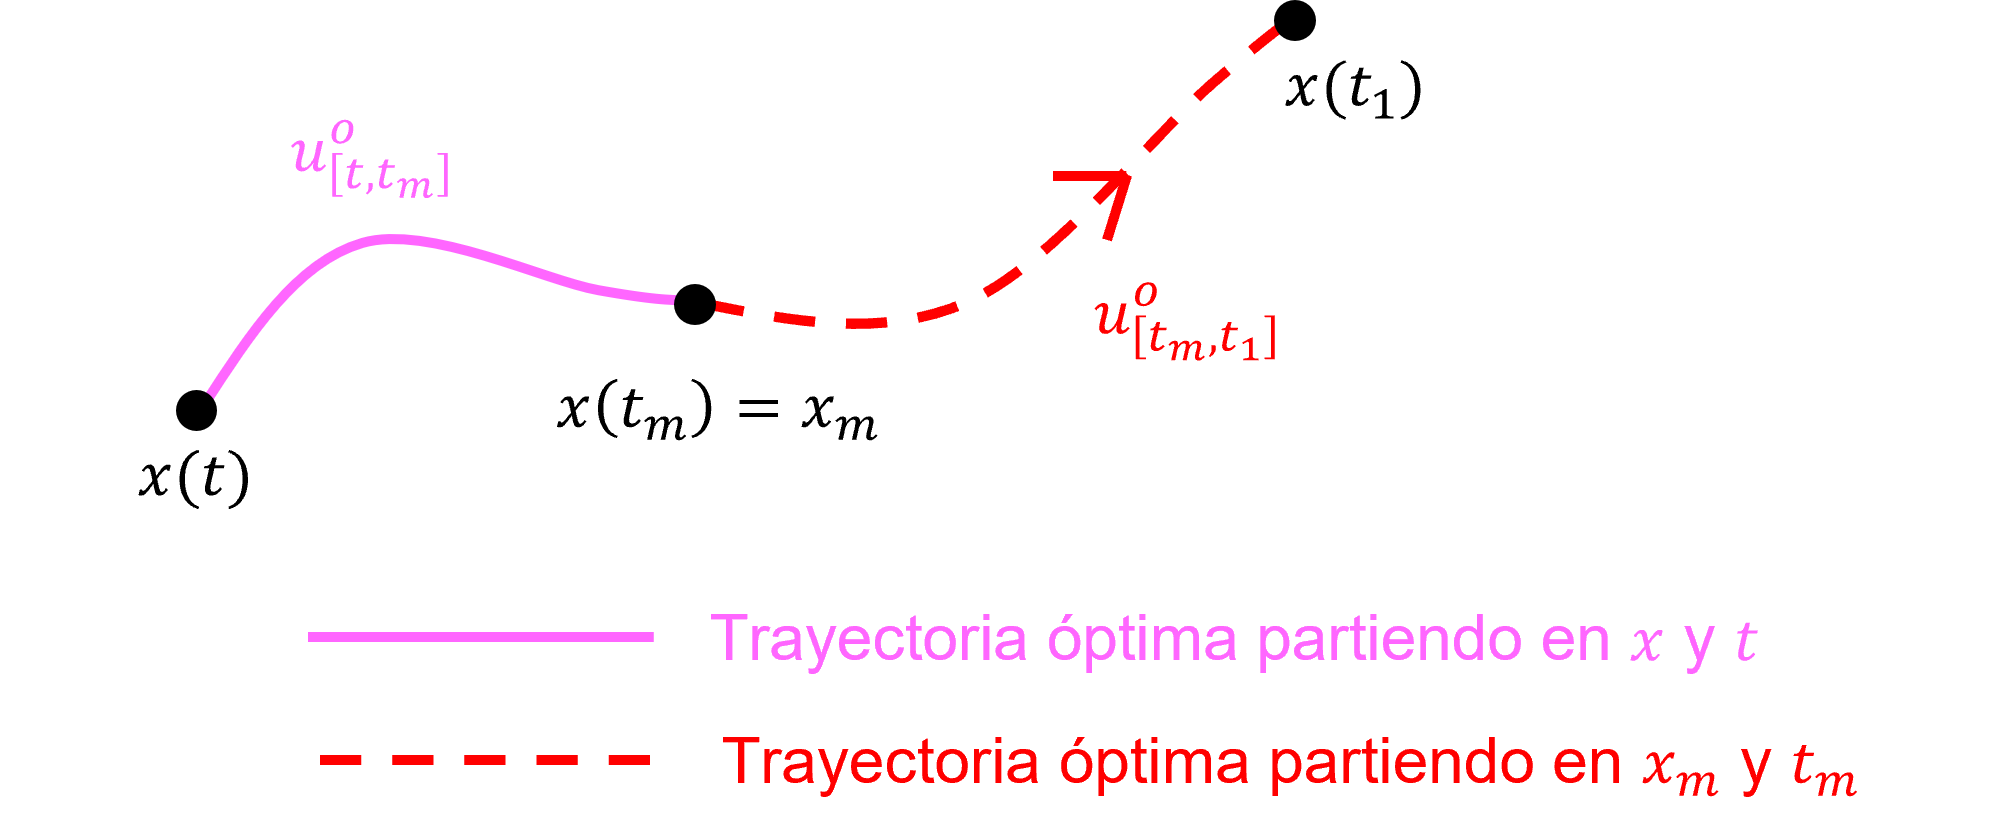
\includegraphics[scale=0.7]{Figuras/optimalidad.png}
\end{figure}

\section{Ecuación HJB (Hamilton-Jacobi-Bellman)}
Esta ecuación resuelve $V(x,t)$ y se obtiene de la siguiente forma:
\begin{enumerate}
    \item Principio de Optimalidad
    \item Realizar una expansión de Taylor de $V(x+\Delta x,t+\Delta t)$ con respecto a $V(x,t)$
    \item Combinar 1. y 2. y dividir por $\Delta t$
    \item Calcular límite para $\Delta t\to 0$
\end{enumerate}

\begin{align*}
    \text{Ec. HJB: } \quad -V_t(x,t) = \min_{u \in \mathcal{U}} \left\{ l(x,u,t) + \left( \nabla_x  V(x,t) \right)^T f(x,u,t) \right\}
\end{align*}

donde $V_t=\frac{\partial V}{\partial t}$, $\nabla_xV=\frac{\partial V}{\partial \tend{x}}$ \\
\par Notar que la ecuación HJB es una ec. diferencial parcial. Por lo tanto, para resolver necesitamos condiciones de borde:
\begin{align*}
    V\big(x(t_1),t_1\big)=m\big(x(t_1)\big)
\end{align*}

\underline{Definición}: Hamiltoniano
\begin{align*}
    H(x,p,u,t) = l(x,u,t)+p^\top (x,t)f(x,u,t)
\end{align*}
donde $p(x,t)=\nabla_x V(x,t)$\\

\par Entonces, la ex. HJB se reduce a:
\begin{align*}
    -V_t(x,t)=\min_{u\in\mathcal{U}}H(x,p,u,t)
\end{align*}
Con estas herramientas, formulamos el siguiente algoritmo para diseñar controladores óptimos:
\begin{enumerate}
    \item Construir el Hamiltoniano
    \item Construir la ec. HJB
    \item Buscar $u^o=\text{arg min}_u H(x,p,u,t)$
    \item Substituir $u^o$ en la expresión HJB
    \begin{align*}
        -V_t=H(x,p,u^o,t)
    \end{align*}
    \item Resolver la ec. dif. parcial para determinar $u^o$
\end{enumerate}

\section{Control LQR (Linear Quadratic Regulator)}
Sea el sistema LTI:
\begin{align*}
    \dot{x}=Ax+Bu=f(x,u)
\end{align*}
y el funcional de desempeño:
\begin{align*}
    J(u)=\int_{t_0}^{t_1}[x^\top Q x+u^\top Ru]dt+x^\top(t_1)Mx(t_1)
\end{align*}
Requisitos: $Q$, $R$, $M$ son matrices definidas positivas y simétricas.\\
\par Utilizando el algoritmo para resolver la ec. HJB:
\begin{enumerate}
    \item[1.] Hamiltoniano:
    \begin{align*}
        H(x,u,V_x,t)=x^\top Qx+u^\top Ru+V^\top_x(Ax+Bu)
    \end{align*}
    \item[3.] Buscar $u^o$: $u^o=\text{arg min}_u H(x,u,V_x,t)$
    \begin{align*}
        \Longrightarrow \frac{\partial H}{\partial u}=0 \Longrightarrow \frac{\partial}{\partial u}[[x^\top Q x+u^\top Ru +V_x^\top(Ax+Bu)]=0\\
        \Longrightarrow 2Ru+B^\top V_x=0\\
        \Longrightarrow u^o=\frac{-1}{2}R^{-1}B^\top V_x(x,t)
    \end{align*}
    \item[2. y 4.] \begin{align*}
        -V_t(x,t) &= H(x,u^o,V_t,t)\\
        \Longrightarrow -V_t &= x^\top Qx+(u^o)^\top Ru^o+V_x^\top (Ax+Bu^o)
    \end{align*} 
    \begin{align}
        \Longrightarrow -V_t &= x^\top Qx-\frac{1}{4}V_x^\top BR^{-1}B^\top V_x+V_x^\top Ax
    \end{align}
\end{enumerate}

Suponga que: $V(x,t)=x^\top P(t)x$, $P(t)\in \mathbb{R}^{n\times n}$, $P^\top (t)=P(t)$, $P(t)\succ 0$
\begin{align*}
    V_t &= x^\top \dot{P}(t)x\\
    V_x &= 2P(t)x
\end{align*}

Sustituyendo en (12):
\begin{align*}
    -x^\top \dot{P}x &= x^\top Qx-\frac{1}{4}(2Px)^\top BR^{-1}B^\top (2Px)+(2Px)^\top Ax\\
    \Longrightarrow -x^\top \dot{P}x &= x^\top\left[Q +PA+A^\top P-P^\top BR^{-1}B^\top P \right]x\\
    \Longrightarrow \dot{P} &= Q +PA+A^\top P-P^\top BR^{-1}B^\top P \quad \text{Ec. diferencial de Riccati}
\end{align*}

Resuelto $P(t)\Longrightarrow V(x,t)=x^\top P(t)x$
\begin{align*}
    V_x(x,t) &= 2P(t)x\\
    \Longrightarrow u^o &= 1\frac{1}{2}R^{-1}B^\top V_x(x,t) = -1\frac{1}{2}R^{-1}B^\top (2P(t)x)\\
    u^o &= -R^{-1}B^\top P(t)x\\
    u^o &= -K(t)x
\end{align*}

donde $K(t)=R^{-1}B^\top P(t) \Longrightarrow$ Control óptimo LQR de horizonte finito (gains variable en el tiempo)
\begin{figure}[H]
\centering
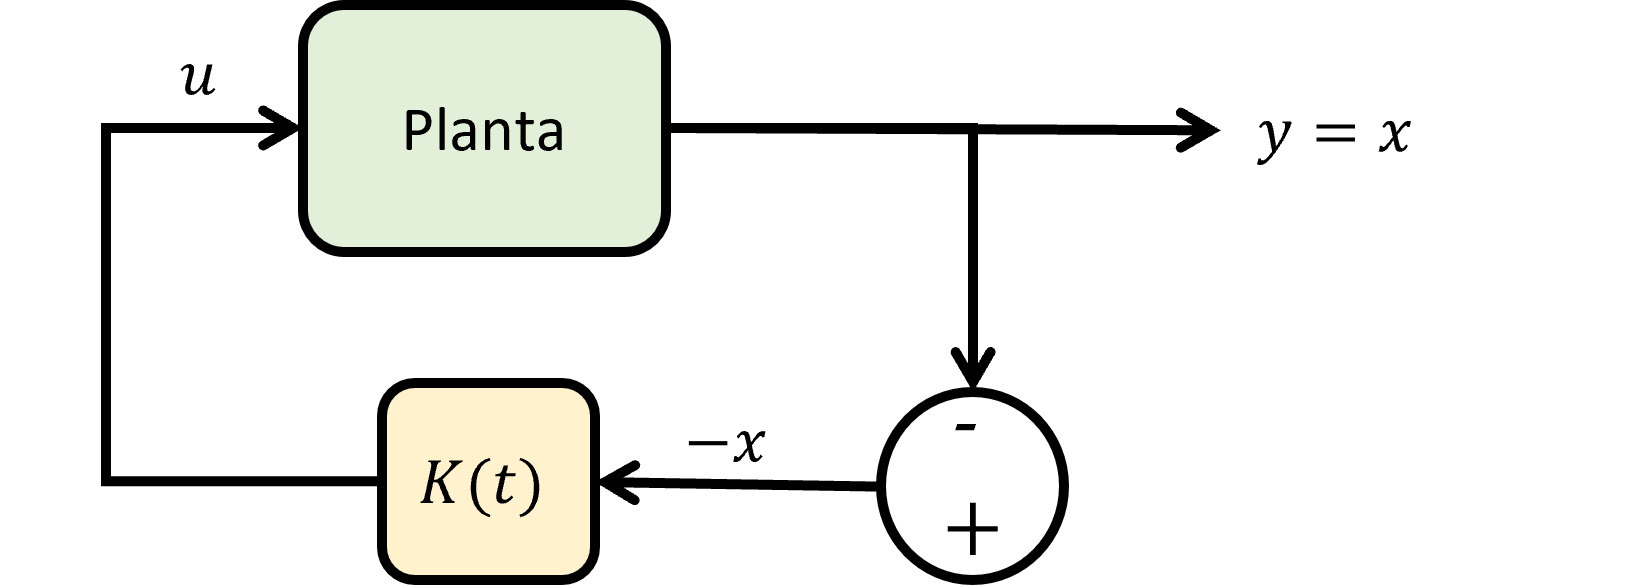
\includegraphics[scale=0.7]{Figuras/LQR.png}
\end{figure}

\section{Control LQR de horizonte infinito}
Dado el sistema LTI: 
\begin{align*}
    \dot{x}=Ax+Bu
\end{align*}
Asumiendo que el sistema es:
\begin{itemize}
    \item estable y controlable, o
    \item inestable, pero los estados inestables son controlables $\Longrightarrow$ estados estabilizables.
\end{itemize}

El problema de control óptimo LQR en horizonte infinito minimiza el siguiente funcional:
\begin{align*}
    J(u) = \lim_{t_1\to \infty} \left[\int_0^{t_1}(x^\top Qx+u^\top Ru)dt \right]
\end{align*}
\underline{Nota}: En este caso, el costo terminal se asume igual a 0.\\
\par Según la lección anterior:
\begin{align*}
    V^{t_1}(x,t)=x^\top P(t,t_1)x \quad \text{: Función de valor para horizonte finito ``$t_1$''}
\end{align*}

Para resolver $P(t,t_1)$, utilizamos la DRE (Differential Riccati Equation):
\begin{align*}
    -\dot{P}=Q+PA+A^\top P-P^\top BR^{-1}B^\top P
\end{align*}
Con condiciones de borde: $P(t_1,t_1)=m(x(t_1))=0$ (costo terminal)\\
\par Finalmente: $u^o(t,t_1)=-R^{-1}B^\top P(t,t_1)x(t)$, con $K(t,t_1)=R^{-1}B^\top$.\\
\par En el límite cuando $t_1\to\infty$, $P(t)$ tiende a una solución de estado estacionario:
\begin{align*}
    \lim_{t_1\to\infty}P(t,t_1)&=P=\text{constante}\\
    \lim_{t_1\to\infty}\dot{P}(t,t_1)&=0
\end{align*}

Entonces, aplicando este supuesto sobre la DRE:
\begin{align*}
    \lim_{t_1\to \infty} \Big[-\dot{P}(t,t_1) &= P(t,t_1)A+A^\top P(t,t_1)+A-P^\top (t,t_1)BR^{-1}B^\top P(t,t_1)  \Big] \\
    \Longrightarrow 0 &= PA+A^\top P+Q-P^\top BR^{-1}B^\top P \quad \text{: Ecuación Algrebaica de Riccati (ARE)}
\end{align*}

Entonces, la función de valor para horizonte infinito:
\begin{align*}
    \hat{V}(x)=x^\top Px
\end{align*}
donde $P$ es la solución de ARE.
\begin{align*}
    \Longrightarrow u^o &= -R^{-1}B^\top Px(t)\\
    &= -K(t)x(t)
\end{align*}
\begin{itemize}
    \item $K=R^{-1}B^\top P$: Gain control LQR horizonte infinito.
\end{itemize}
Finalmente, se puede demostrar que:
\begin{align*}
    V^{t_1}(x,t) \leq J(u)
\end{align*}
\begin{itemize}
    \item $V^{t_1}(x,t)$: Función de valor para horizonte finito $t_1$.
    \item $J(u)$: Funcional de desempeño para horizonte infinito.
\end{itemize}

\subsection{Heurística de diseño}
\par P: ¿Cómo elijo los valores de $Q$ y $R$? 
\par R: Recordar que
\begin{align*}
    J(u) = \int_0^\infty \Big( x^\top Qx+u^\top Ru\Big) dt
\end{align*}
\par Recordar que en sistemas estructurales:
\begin{align*}
    x = \left[
    \begin{array}{c}
     \dot{z} \\ \dot{z} 
    \end{array}\right]
\end{align*}

\begin{itemize}
    \item $z$: desplazamiento
    \item $\dot{z}$: velocidad
\end{itemize}

Podemos escribir la forma cuadrática $x^\top Q x$ de manera tal que le asignamos un significado físico:
\begin{align*}
    \frac{1}{2}x^\top Qx=\frac{1}{2}\left[
    \begin{array}{cc}
     \dot{z} & \dot{z} 
    \end{array}\right] \left[
    \begin{array}{cc}
     K_s & \emptyset \\ \emptyset & M_s 
    \end{array}\right] \left[
    \begin{array}{c}
     \dot{z} \\ \dot{z} 
    \end{array}\right] = \frac{1}{2}z^\top K_s z+\frac{1}{2}\dot{z}^\top M\dot{z}
\end{align*}
\begin{itemize}
    \item $\frac{1}{2}z^\top K_s z$: Energía potencial
    \item $\frac{1}{2}\dot{z}^\top M\dot{z}$: Energía cinética
\end{itemize}

Por otra parte: $u^\top Ru$: energía consumida por el controlador.
\par \underline{Comentario}: No importan los valores absolutos de $Q$ y $R$ en el resultado del control óptimo. Lo que s;i importan son los valores relativos de $Q$ respecto a $R$ (o viceversa).
\begin{align*}
    J(u)=\int_0^\infty (x^\top Qx+u^\top Ru)dt
\end{align*}

\begin{itemize}
    \item $Q$ es mayor que $R$: resultado es sensible a los estados. \\
    \underline{Nota}: Si $R\to 0$: control ``barato'' (cheap) LQR. No es recomendable. \\
    $K=R^{-1}B^\top P$: valor muy grande.
    \item $R$ es mayor que $Q$: resultado es sensible a la señal de control.
\end{itemize}

\subsection{Regla de Bryson}
Elegir $Q$ y $R$ matrices diagonales. Cada componente de $q_{ii}$ y $r_{ii}$ están dados por:
\begin{align*}
    q_{ii} &= \frac{1}{\text{máx valor aceptable de }x_i^2}\\
    r_{ii} &= \frac{1}{\text{máx valor aceptable de }u_i^2}
\end{align*}



\section{Filtro de Kalman (continuo)}
Sea el sistema LTI
\begin{align*}
    \dot{x} &= Ax+B_u u +B_\omega \omega(t)\\
    y &= Cx+v(t)
\end{align*}

donde $\omega$ es la perturbación sobre el sistema y $v$ es el ruido de la medición.\\

\begin{figure}[H]
\centering
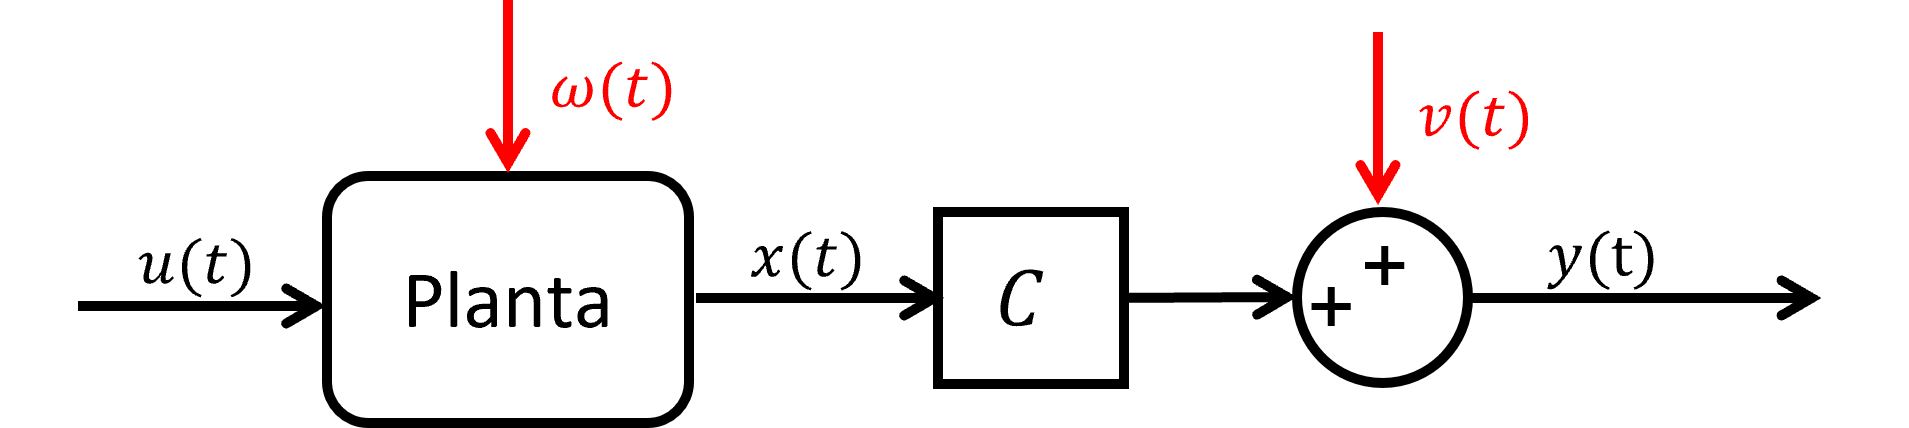
\includegraphics[scale=0.7]{Figuras/wv.png}
\end{figure}

\par \underline{Objetivo}: Estimar los estados $x$ utilizando un observador.\\
\par \underline{Condición}: 
\begin{itemize}
    \item (C,A) es observable
    \item A es Hurwitz
    \item $\Longrightarrow$ Estados detectables
\end{itemize}

Asumir que $\omega (t)$ y $v(t)$ son p.e. Gaussianos, w.s.s., y de media cero:

\begin{itemize}
    \item Perturbación, $\omega (t)$: \begin{itemize}
        \item $\mathbb{E}\{\omega (t)\}=0$
        \item $\mathbb{E}\{\omega (t) \omega^\top (s)\}=Q_\omega \delta(t-s)$
    \end{itemize}
    \item Ruido, $v(t)$: \begin{itemize}
         \item $\mathbb{E}\{v (t)\}=0$
        \item $\mathbb{E}\{v (t) v^\top (s)\}=R_v \delta(t-s)$
    \end{itemize}
\end{itemize}

Asumir en el caso particular que:
$$\mathbb{E}\{\omega(t)v^\top (s)\}=0 \Longrightarrow \text{$\omega(t)$ y $v(t)$ están descorrelacionados} $$

Diseñar un observador óptimo $\Longrightarrow$ Filtro de Kalman.

\begin{figure}[H]
\centering
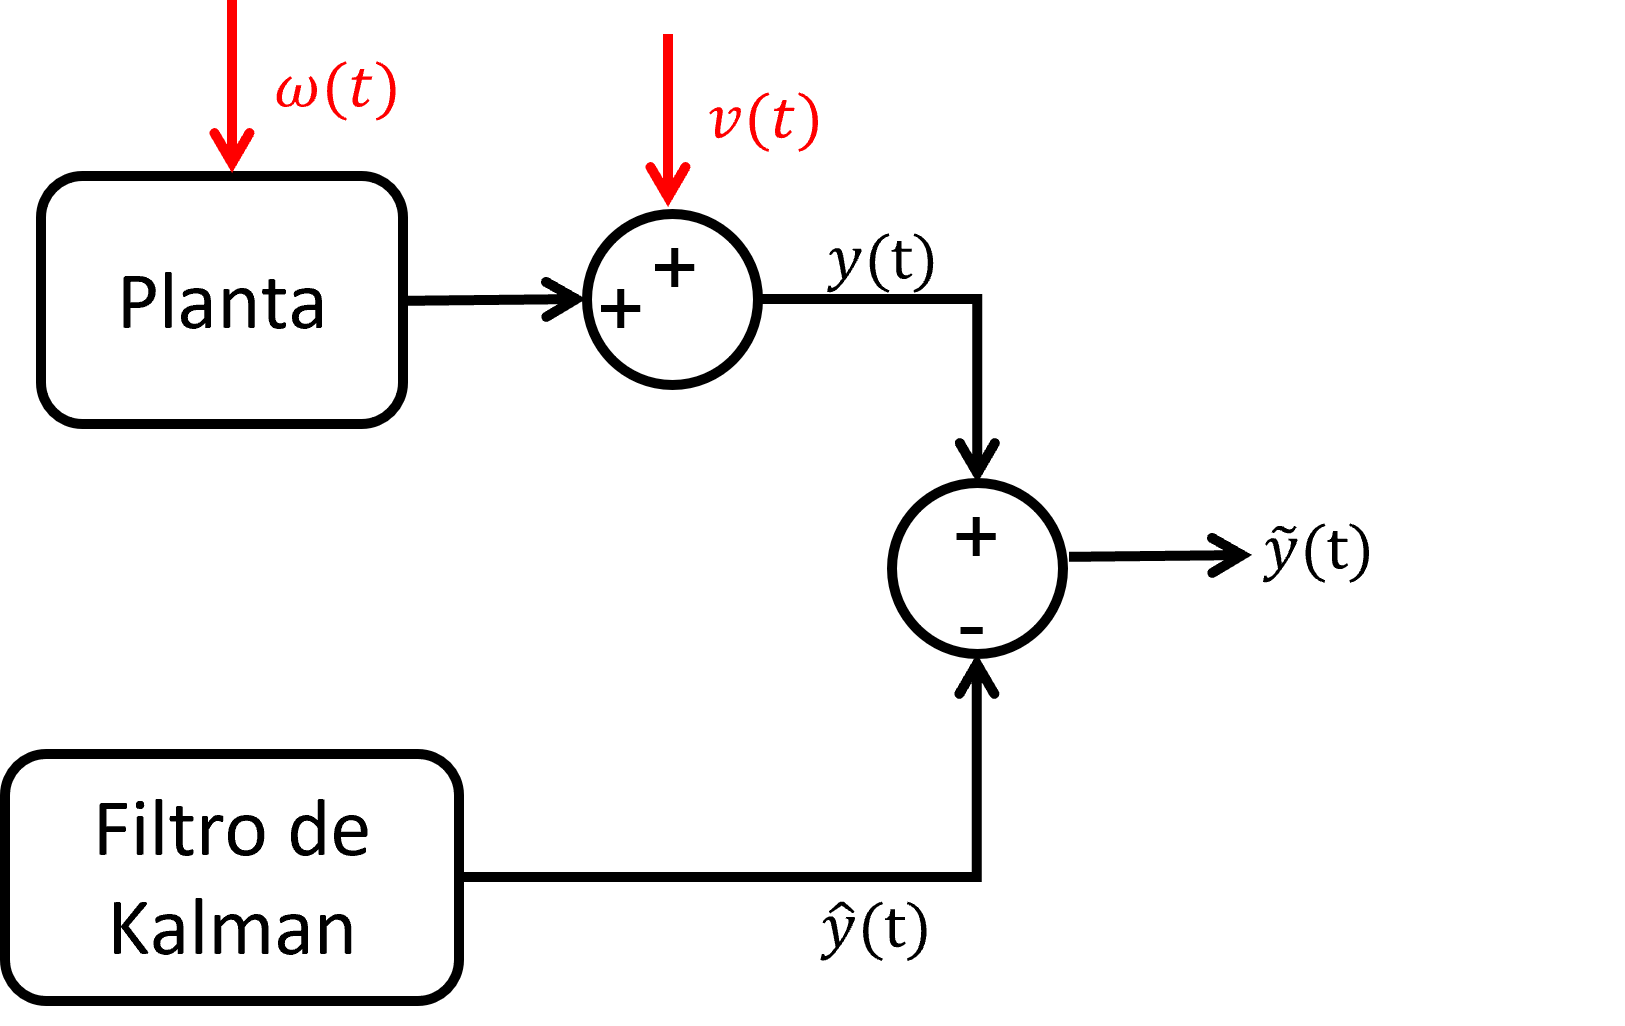
\includegraphics[scale=0.7]{Figuras/Kalman.png}
\end{figure}

\par Problema: 
\begin{align*}
    \text{Minimizar } \tilde{y} &= y-\hat{y}\\
    \Leftrightarrow \text{Minimizar } \tilde{x} &= x-\hat{x}
\end{align*}

\underline{Definición}: Matriz de autocovarianza del error de estado $\tilde{x}$ (en estado estacionario) 

\begin{align*}
    \Gamma=\mathbb{E}\{\tilde{x}\tilde{x}^\top \} \text{: matriz cuadrada, simétrica, definida positiva}
\end{align*}

\underline{Problema}: $\min J$, $J=\text{trace}(\Gamma^\top \Gamma)$
$$J=\mathbb{E} \Bigl\{[x_i-\hat{x}_i][x_i-\hat{x}_i]\Bigr\} $$

Los pasos a seguir son análogos al problema de control óptimo LQR de horizonte infinito. 
\begin{enumerate}
    \item La ganancia de Kalman se define como: $L_{KAL}=\Gamma C^\top R_v ^{-1}$
    \item $\Gamma$ se obtiene de resolver la siguiente ecuación algebraica de Riccati: 
    $$A\Gamma+\Gamma A^\top +\bigl(B_\omega Q_\omega B_\omega^\top -\Gamma C^\top R_v^{-1}C\Gamma\bigr)=0 $$
\end{enumerate}

En términos prácticos, este problema se resuelve en Matlab mediante el comando \texttt{Kalman()}
$$(L_{KAL},\Gamma)=\text{Kalman}(A,C,Q_\omega,R_v) $$

Finalmente:
\begin{align*}
    \dot{\hat{x}} &= A\hat{x}+B_u u+L_{KAL}(y-\hat{y})\\
    \hat{y} &= C\hat{x}
\end{align*}

\begin{figure}[H]
\centering
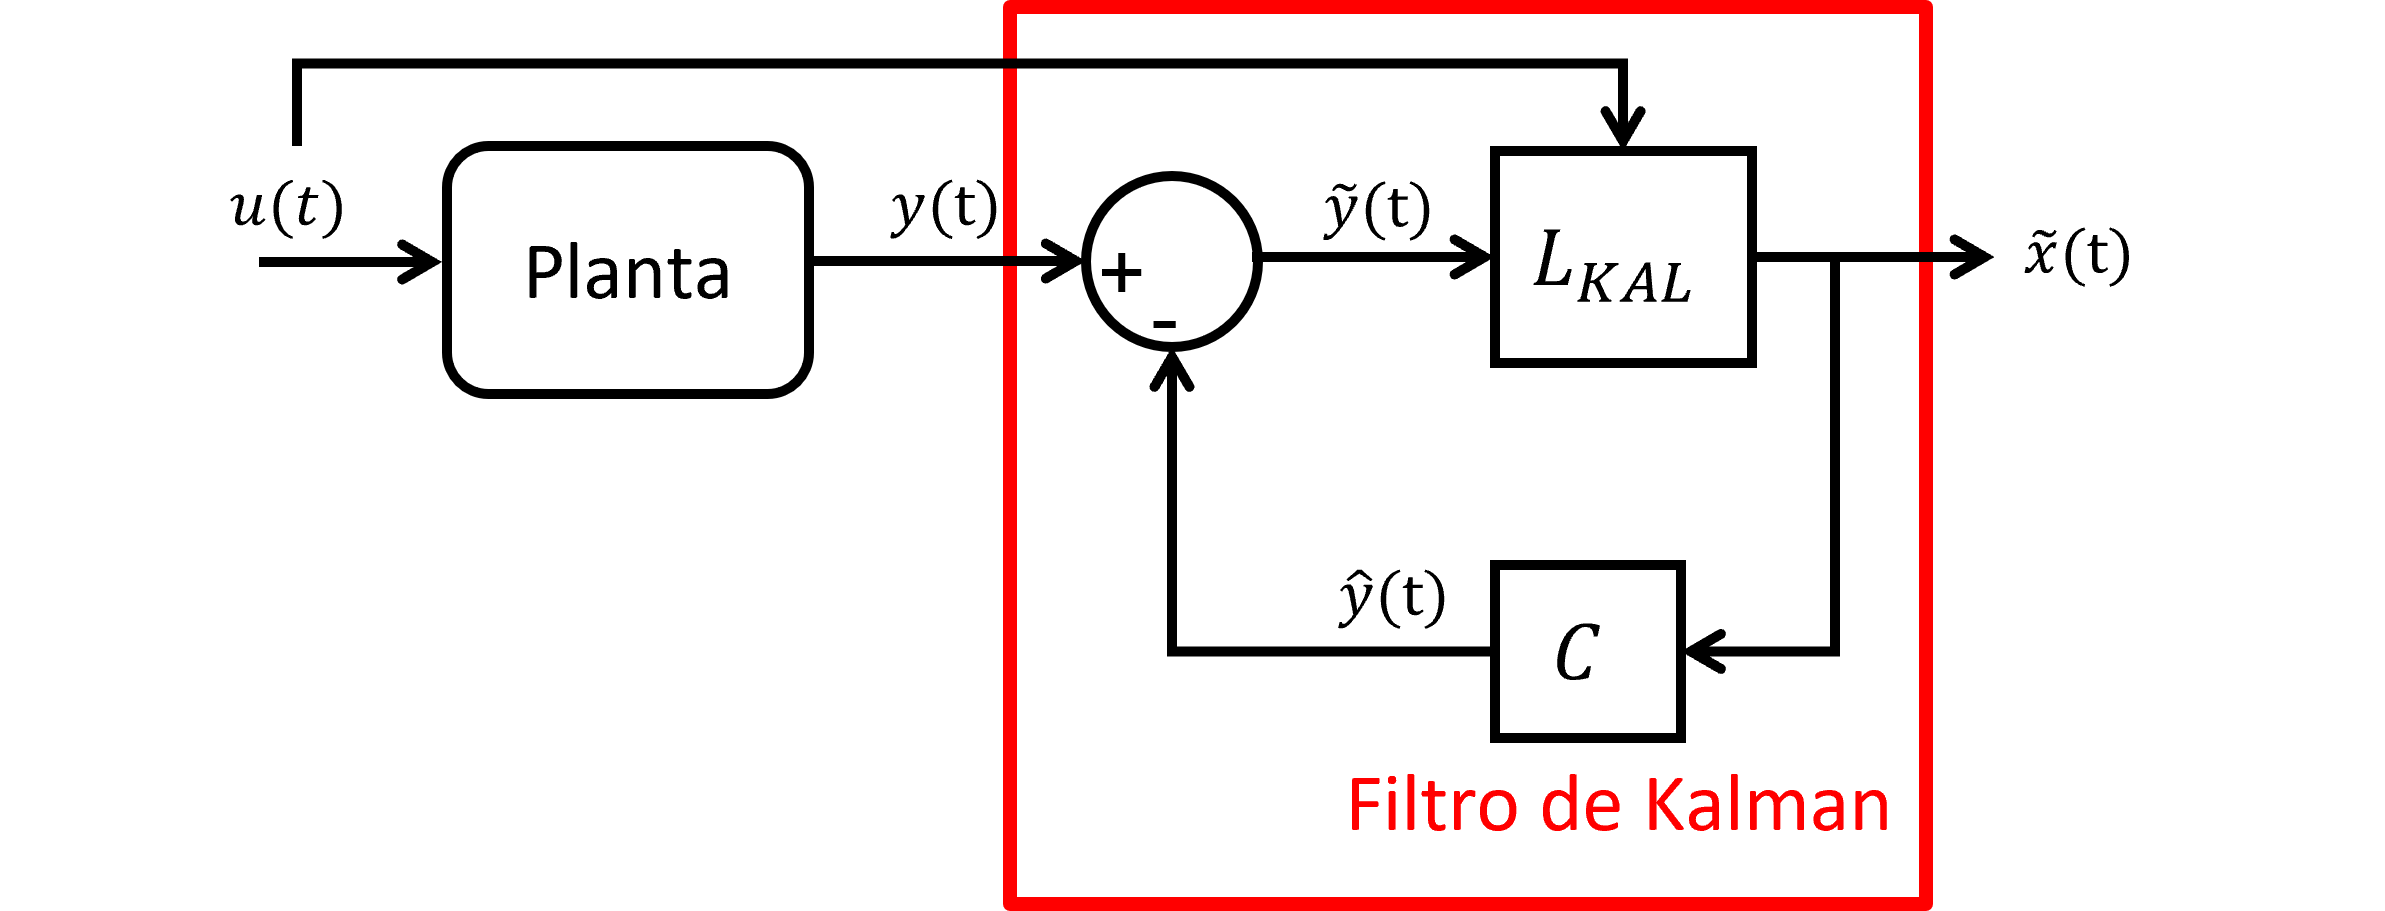
\includegraphics[scale=0.7]{Figuras/Kalman2.png}
\end{figure}

\section{Control LQG}
LQG = Linear Quadratic Gaussian\\
\par Suponga el sistema LTI:
\begin{align*}
    \dot{x} &= Ax+B_u u+B_\omega \omega\\
    y &= Cx+v
\end{align*}

\underline{Objetivo}: diseñar un controlador óptimo con información de la respuesta.

\begin{align*}
    \text{Control óptimo (LQR)} + \text{Obervador óptimo (Kalman)} \overset{\text{Principio de superposición}}{=} LQG
\end{align*}


\begin{figure}[H]
\centering
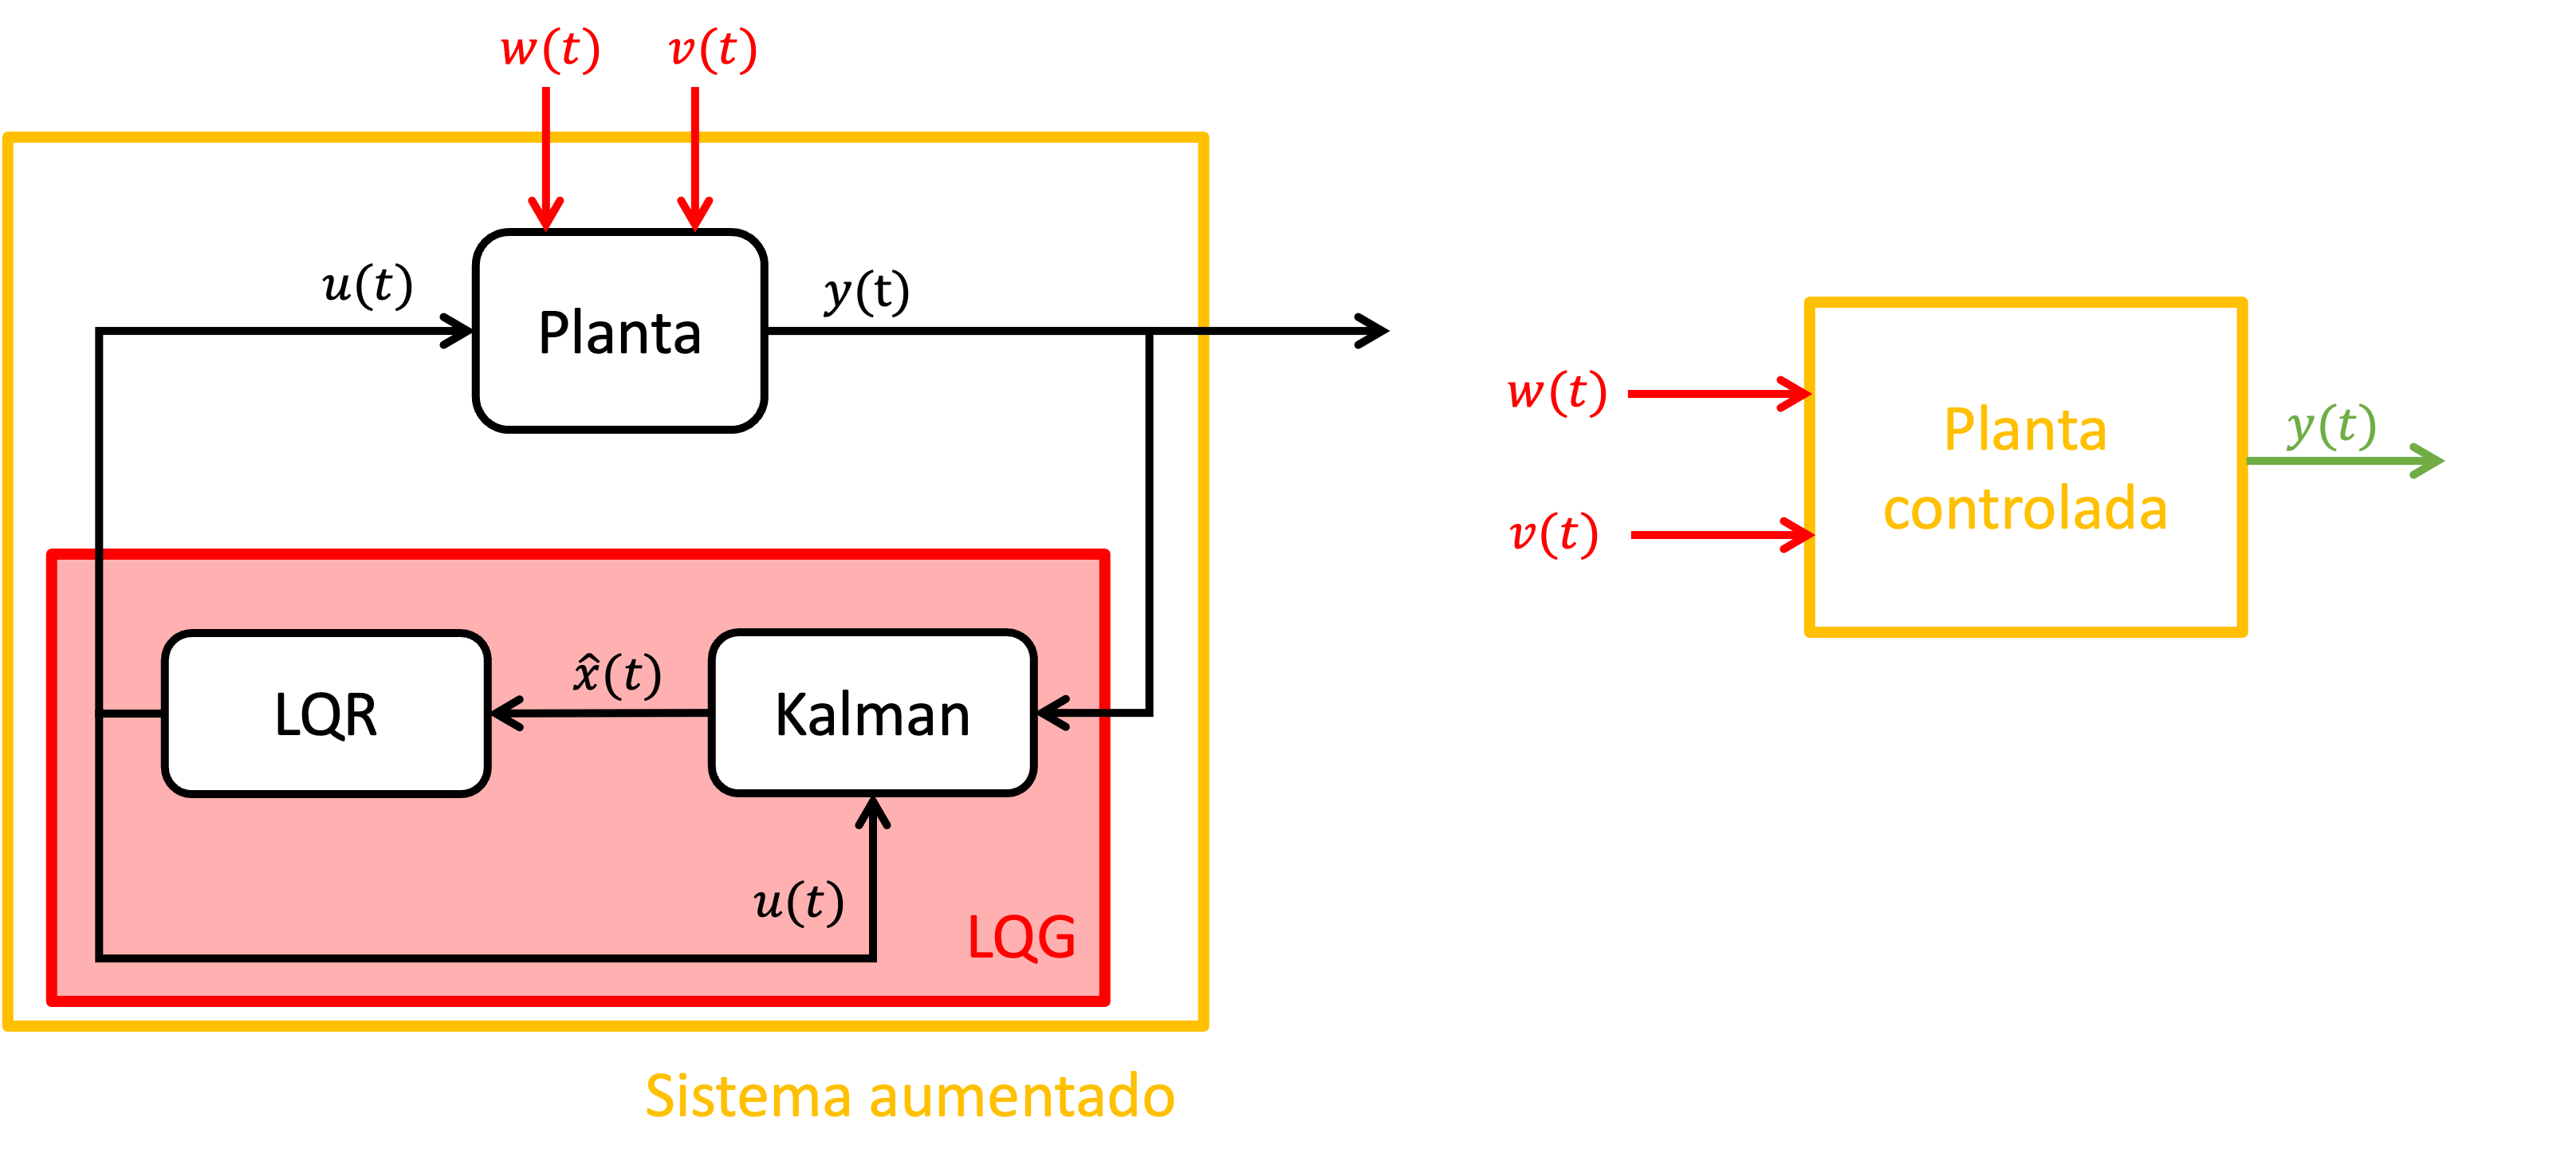
\includegraphics[scale=0.7]{Figuras/LQG.png}
\end{figure}

\underline{Parámetros LQG}: $Q$, $R$, $Q_\omega$, $R_v$.\\


\section{Tópicos especiales en control}

\begin{itemize}
    \item Control robusto (LTR, $H_2$, $H_\infty$, etc.)
    \item Control adaptivo
    \item Control híbrido
    \item Control nolineal
    \item Reinforcement learning
\end{itemize}



\chapter{Tecnología de Sensores y Adquisición Digital de Datos}

% NOTA: Utilizar apuntes de Spencer como guía

\section{Fundamentos básicos de electrónica}

\subsection{Resistencia}

Relación deformación vs voltaje

\subsection{Capacitancia}



\subsection{Piezo-electricidad}

Del griego \emph{piezo} (presión)

\section{Fundamentos de sensores de vibración}

Ecuación de movimiento
FRF: Acelerometro vs Medidor desplazamiento
Giroscopio, efecto de Coriolis
%Ref: https://youtu.be/PK05u9c3yWI?si=s8M-EsRE4FtOPgVj&t=386

\section{Especificaciones de sensores}

\subsection{Sensitividad}

\subsection{Resolución}

\subsection{Rango de frecuencias}

\subsection{Linealidad}

\section{Sensores de vibración}

\subsection{Acelerómetros resistivos}

\subsection{Acelerómetros piezoeléctricos}

\subsection{\emph{Strain gages}}

\subsection{Celdas de carga}

\subsection{Transductores de desplazamiento}

Potenciometros, LVDT, encoders

\subsection{Otros sensores}

Laser interferometer
Gyroscopios % Link: https://youtu.be/DOjT5r4cpNo?si=1dA6Qn6ORPoe-9nk&t=231
Fibra óptica
MEMS
% Link: https://www.analog.com/en/technical-articles/accelerometer-and-gyroscopes-sensors-operation-sensing-and-applications.html
Geofonos
% Link: https://en.wikipedia.org/wiki/Geophone

\section{Adquisición Digital de Datos}

\subsection{Muestreo (\emph{sampling})}

\subsection{Cuantización}

\subsection{Filtros \emph{Anti-Aliasing}}












\chapter{Técnicas de Monitoreo Estructural}

\section{Motivación}

Nunca se está seguro de las propiedades \emph{exactas} de una estructura. 

\begin{enumerate}
    \item Obras civiles ``envejecen'':
    \begin{itemize}
        \item Daño/deterioro estructura $\longrightarrow$ Cambio en las propiedades de materiales
    \end{itemize}
    \item Incertidumbre:
    \begin{itemize}
        \item Propiedades nominales utilizadas en diseño
        \item Los modelos nominales no necesariamente representan fielmente el comportamiento real de la estructura
    \end{itemize}
\end{enumerate}

Un buen proyecto de monitoreo estructural (Structural health monitoring, SHM) tiene múltiples objetivos más allá de la instrumentación.

\begin{figure}[H]
    \centering
    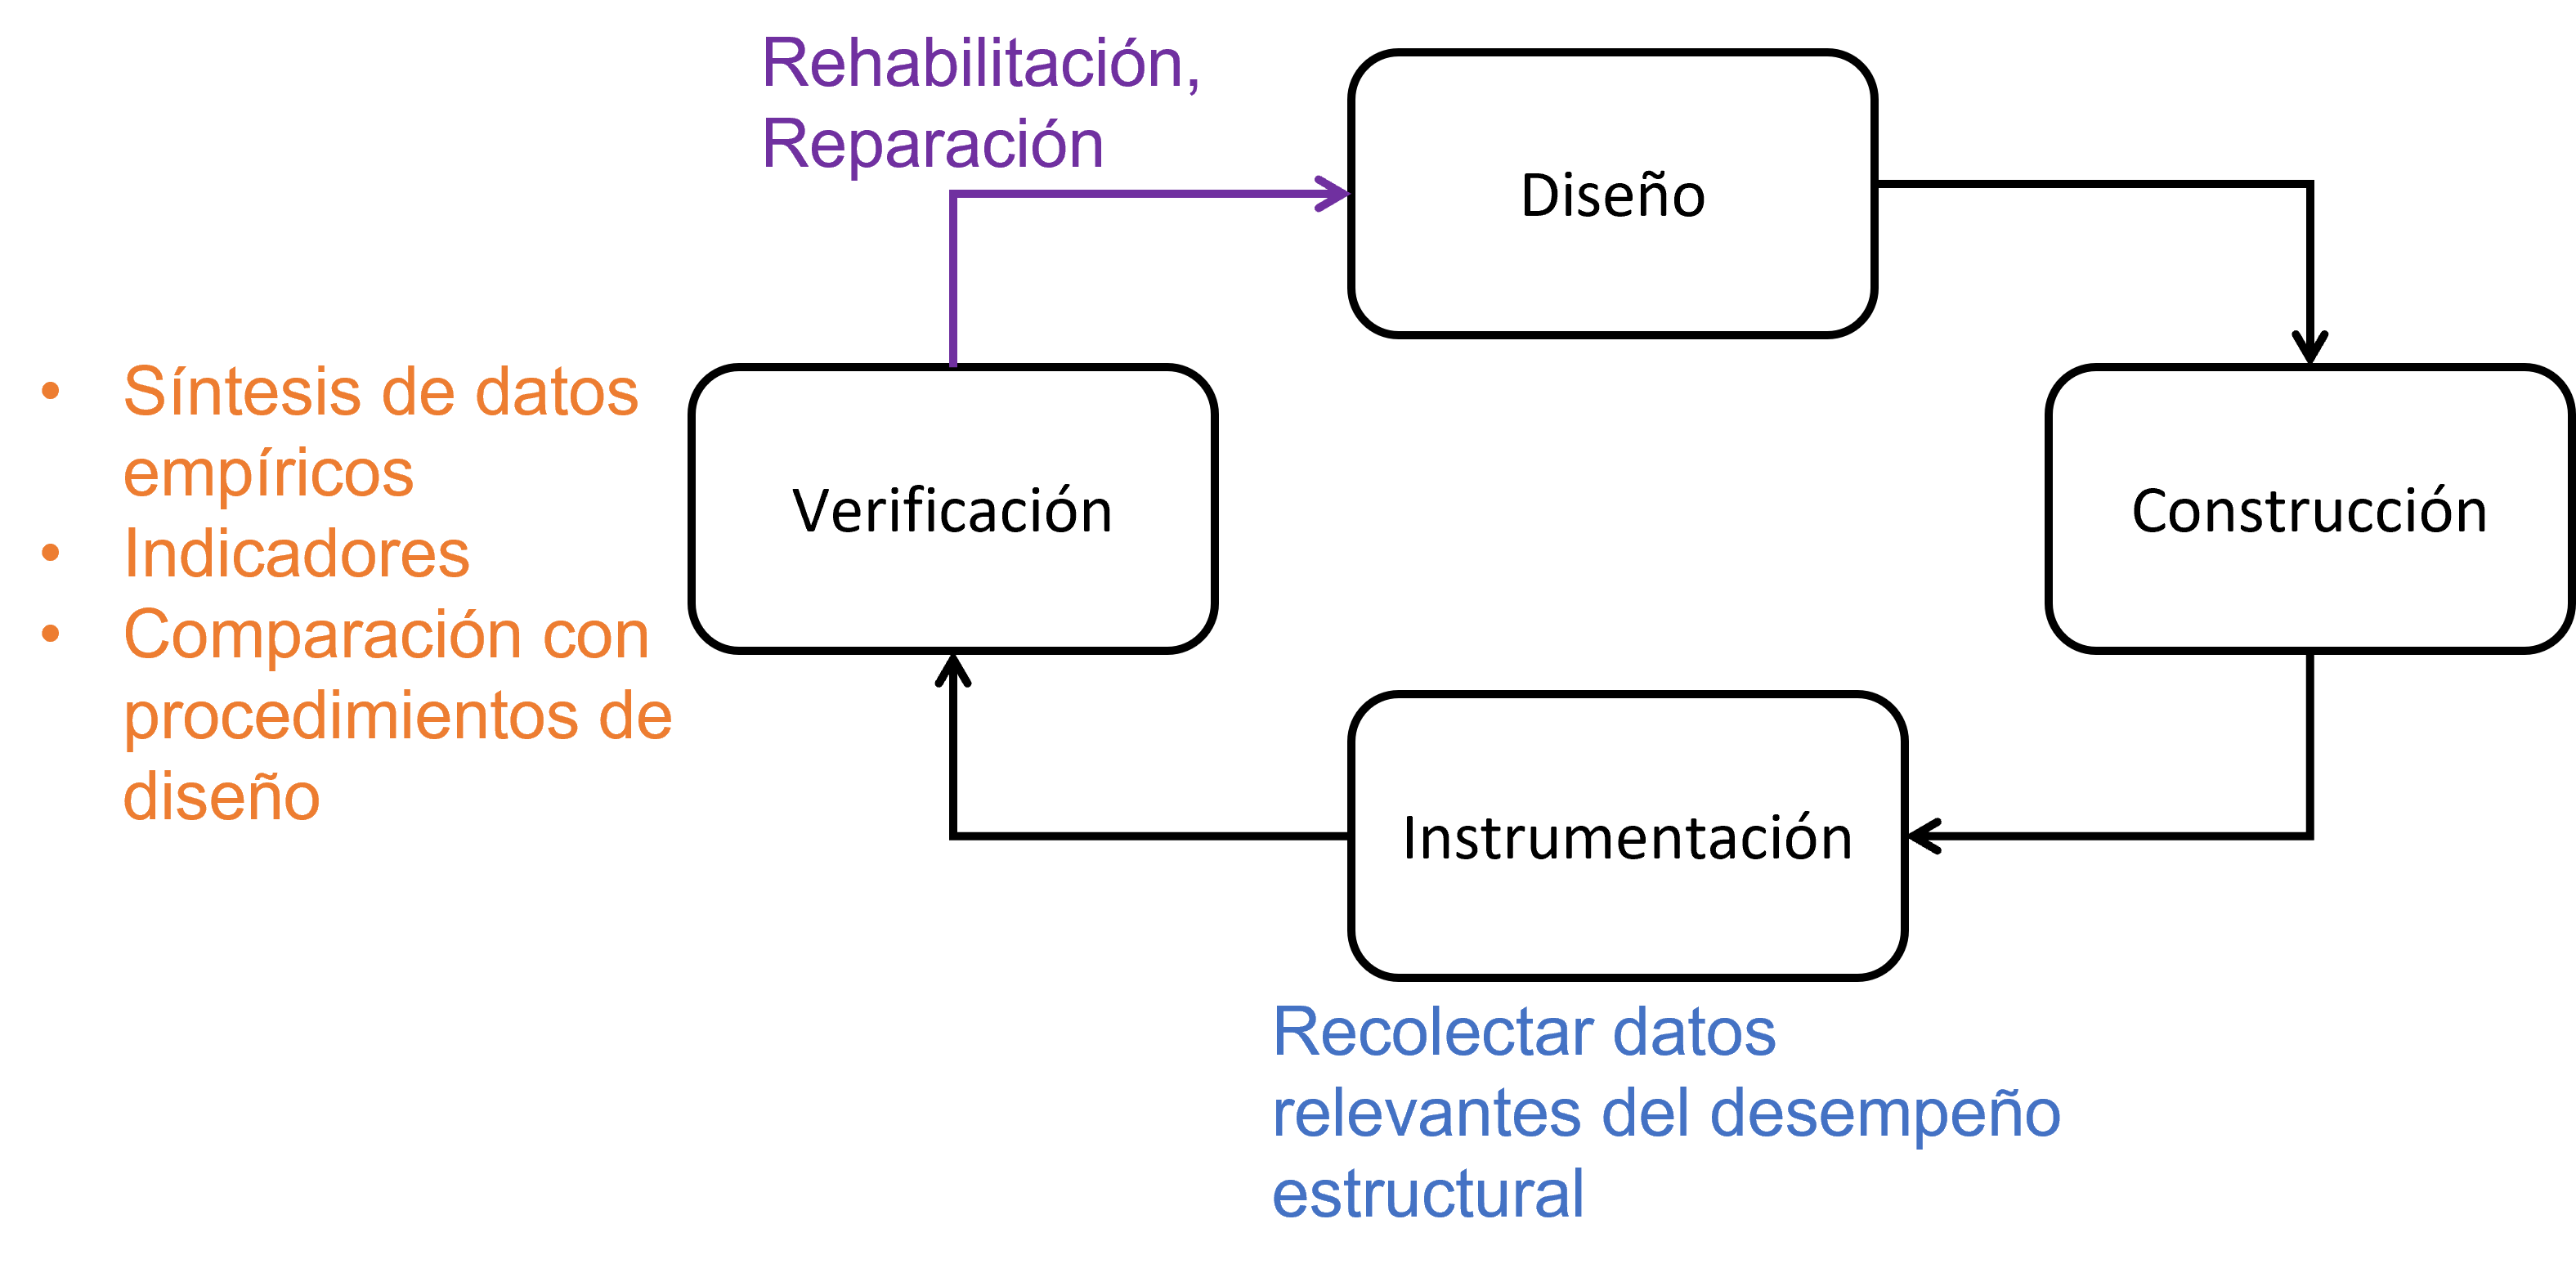
\includegraphics[scale=0.5]{Figuras/sysID.png}
\end{figure}

Para el monitoreo estructural se busca:

\begin{itemize}
    \item Determinar un modelo matemático de un sistema.
    \item Realizar predecicción: desempeño, daño,
\end{itemize}

\section{Identificación de Sistemas}

\subsection{Generalidades}

\begin{enumerate}
    \item Análisis dinámico (problema directo)
    \begin{figure}[H]
    \centering
    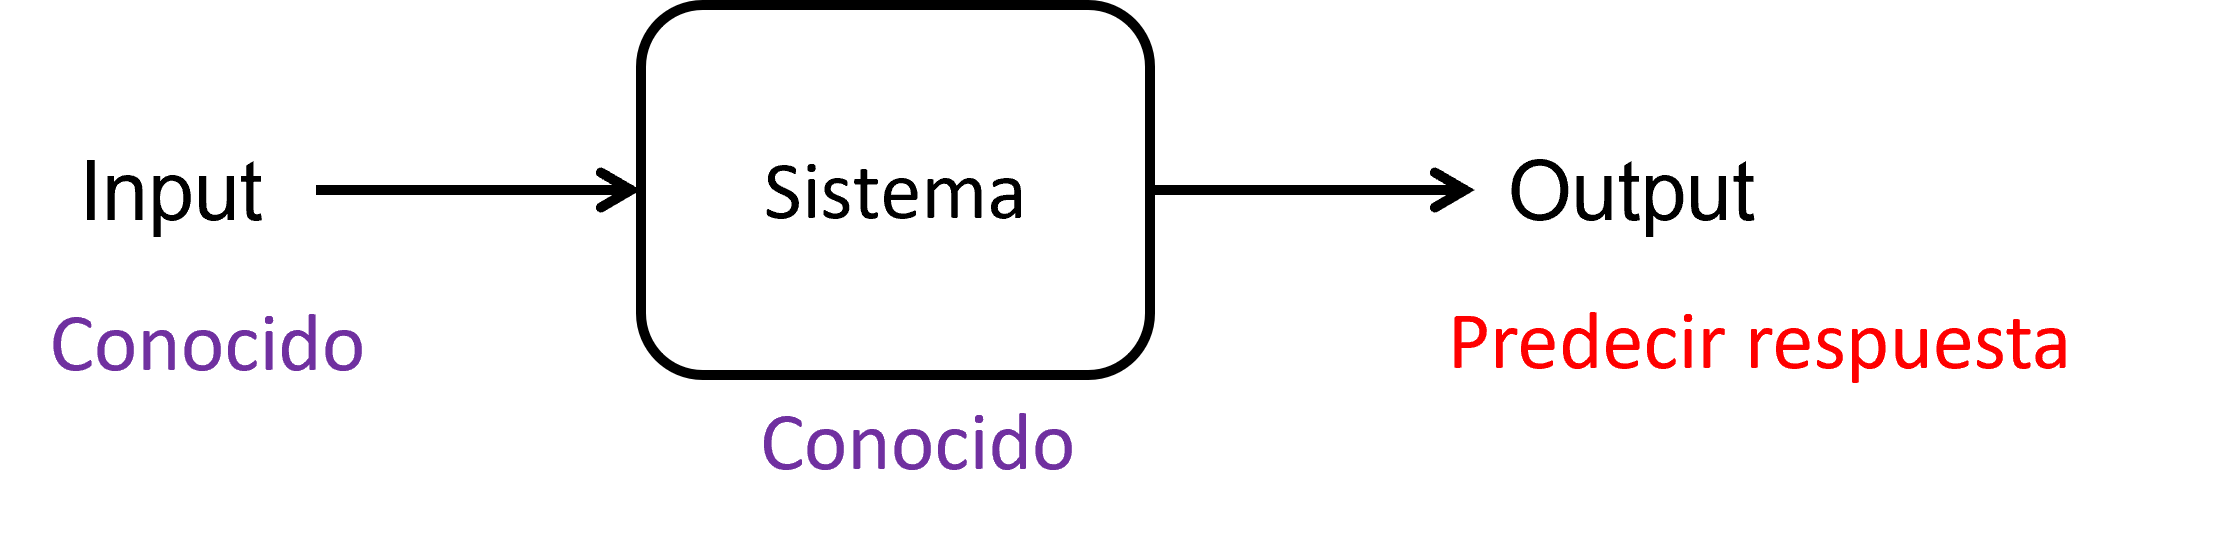
\includegraphics[scale=0.6]{Figuras/problema_directo.png}
    \end{figure}
    \item Identificación de fuerza de entrada
    \begin{figure}[H]
    \centering
    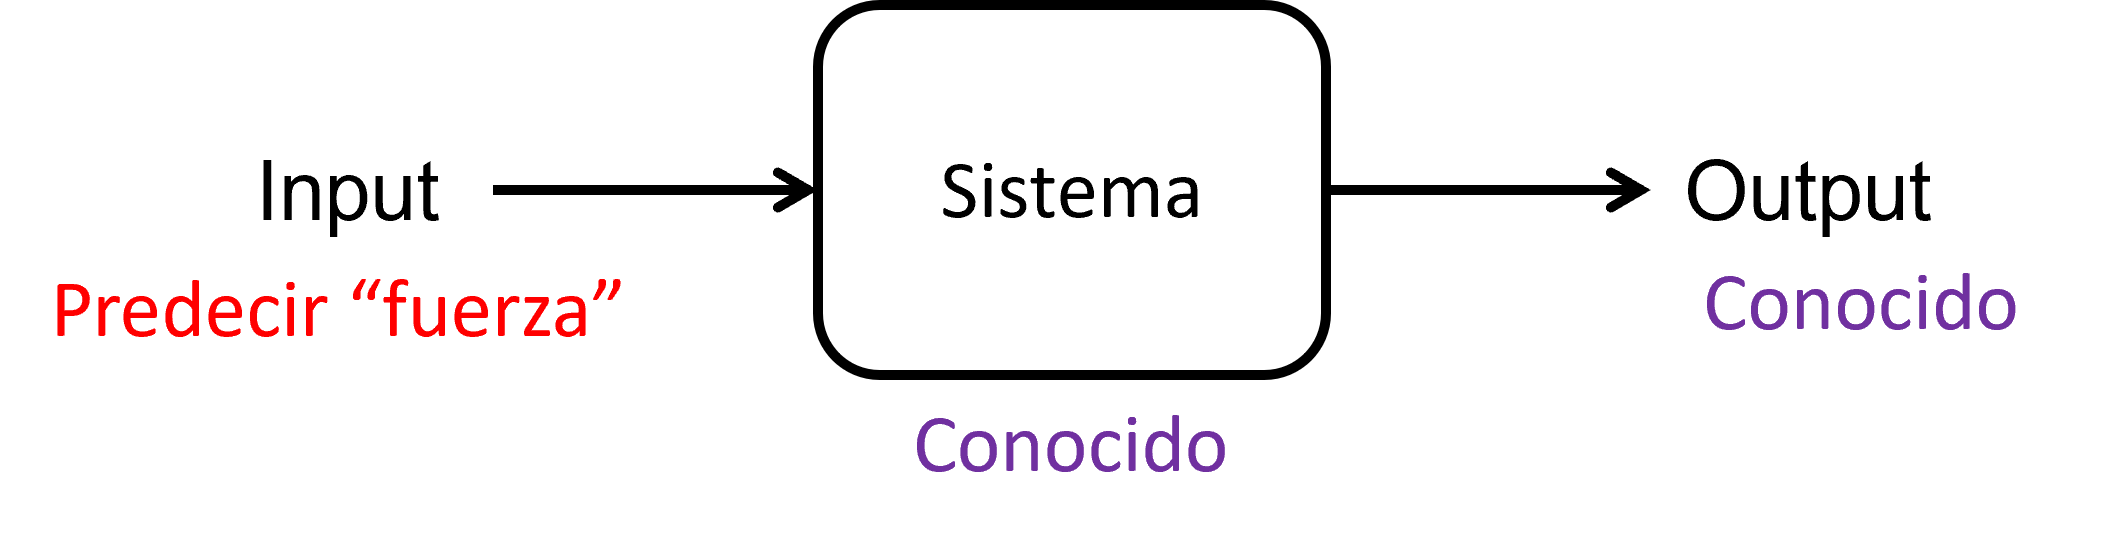
\includegraphics[scale=0.6]{Figuras/fuerza_entrada.png}
    \end{figure}    
    \item Identificación de sistema
    \begin{figure}[H]
    \centering
    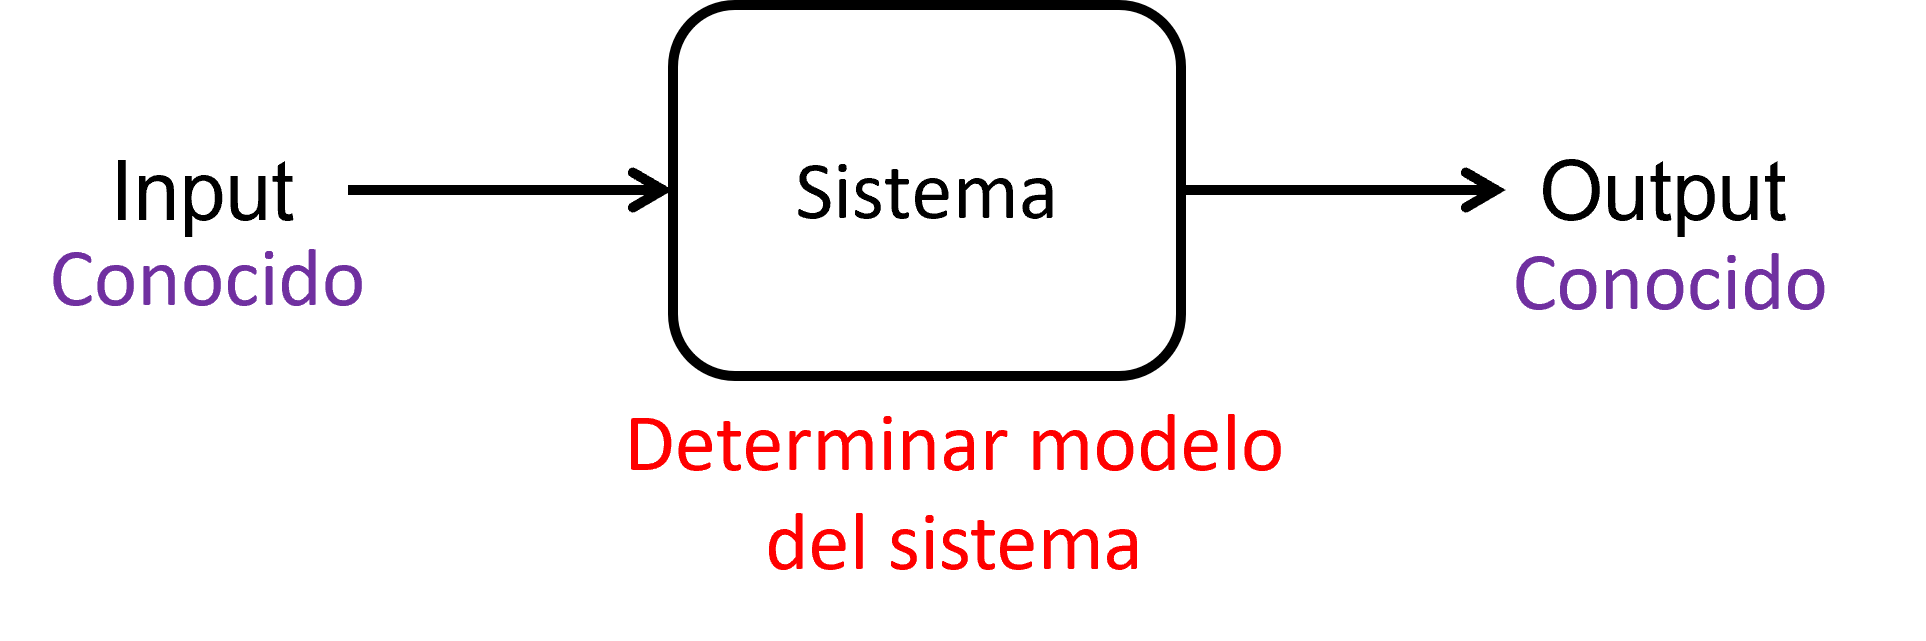
\includegraphics[scale=0.6]{Figuras/problema_inverso.png}
    \end{figure}
\end{enumerate}

Estas predicciones se pueden realizar con distintos métodos:

\begin{enumerate}
    \item Basados en dominio frecuencia
    \begin{itemize}
        \item Análisis modal experimental
        \item Optimización no paramétrica
    \end{itemize}
    \item Basados en dominio tiempo
    \begin{itemize}
        \item Modelos auto-regresivos: ARX, ARMA, ARMAX, etc.
        \item Métodos basados en subespacios: ERA, Next-ERA, SSI, etc.
    \end{itemize}
\end{enumerate}

Resumen de identificación de sistemas (SysID):

\begin{figure}[H]
    \centering
    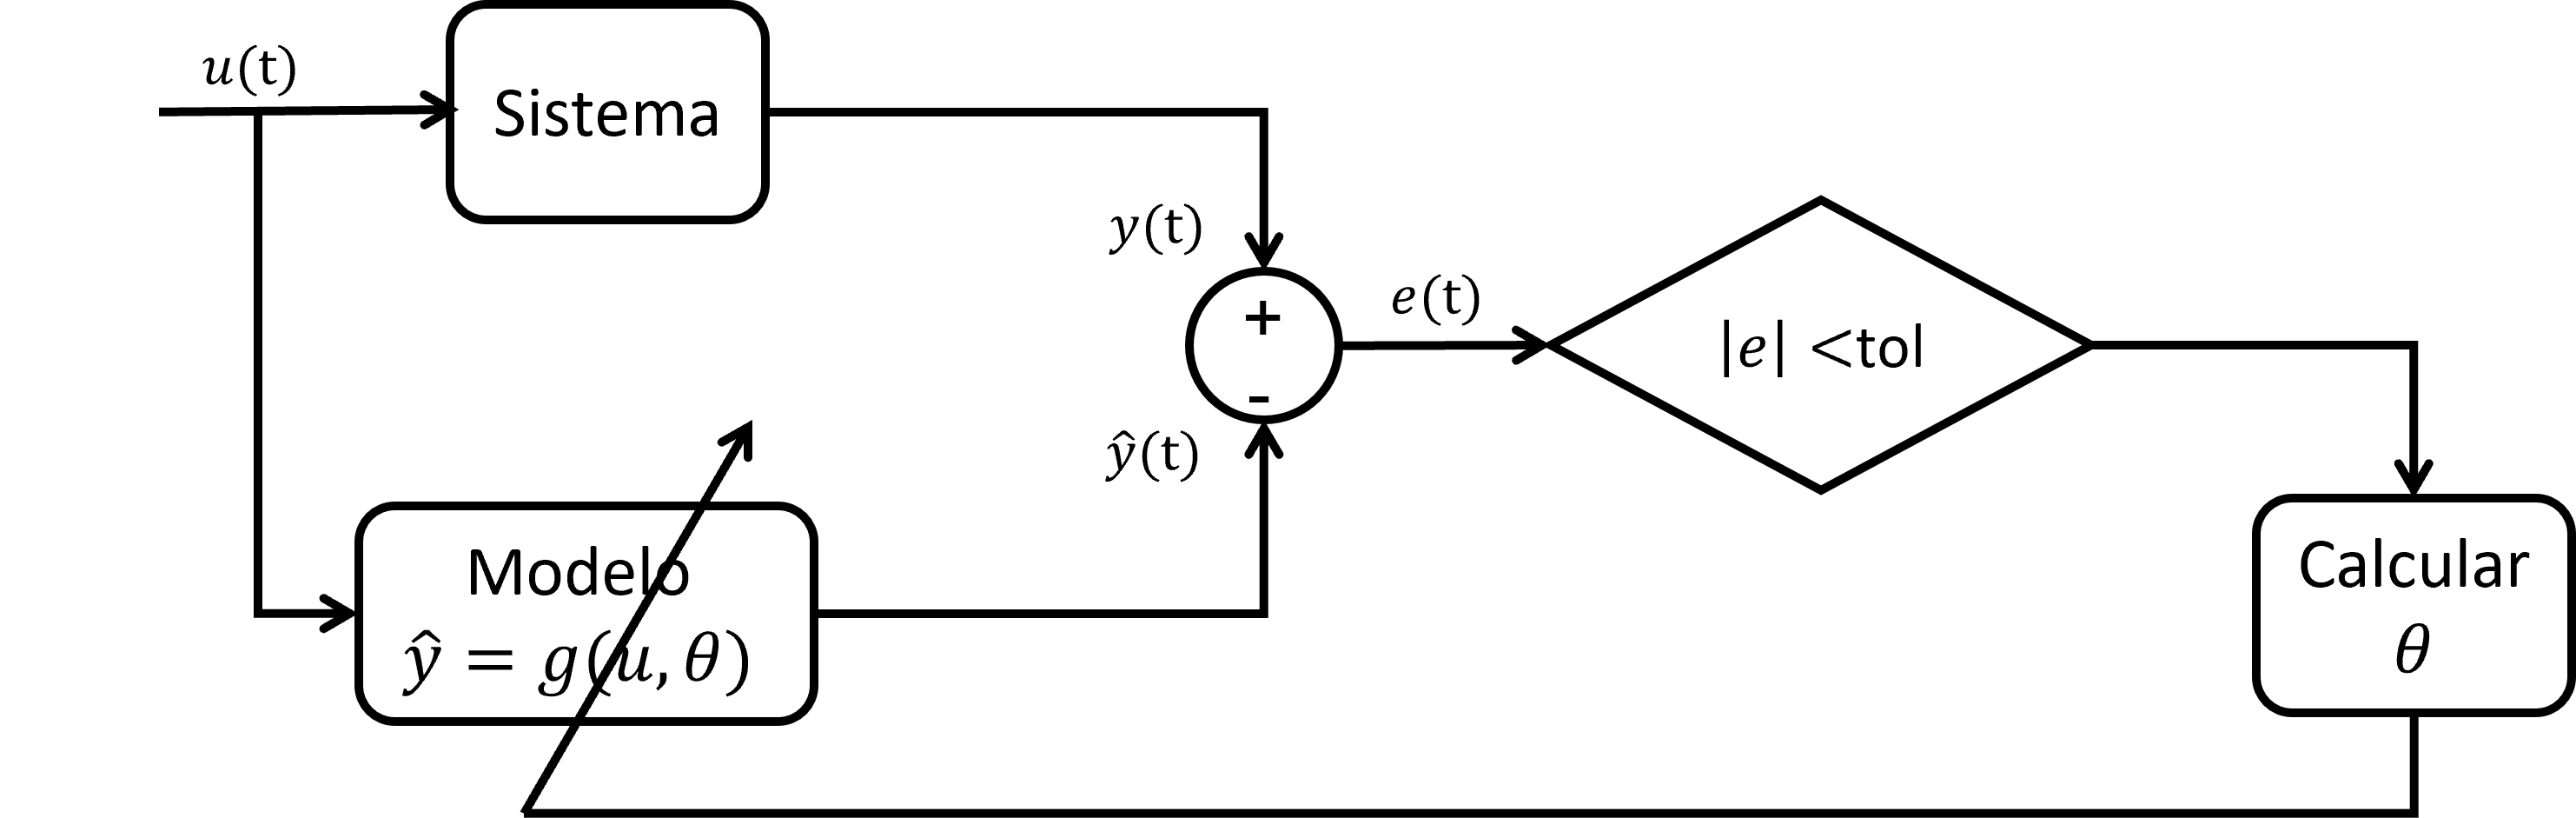
\includegraphics[width=5in]{Figuras/resumenSysID.png}
\end{figure}

\section{Métodos no-paramétricos de estimación espectral}

Referencias: \textcite[Sec. 18.4]{craig2006fundamentalsstructural} y \textcite[Cap. 6]{Bendat2011}. 

\subsection{Definiciones}

Dado un sistema LTI con entrada $u(t)$ y salida $y(t)$ conocidos experimentalmente, buscamos determinar de forma estimada su FRF, $G_{YU}(\omega)$.\\

\begin{figure}[H]
    \centering
    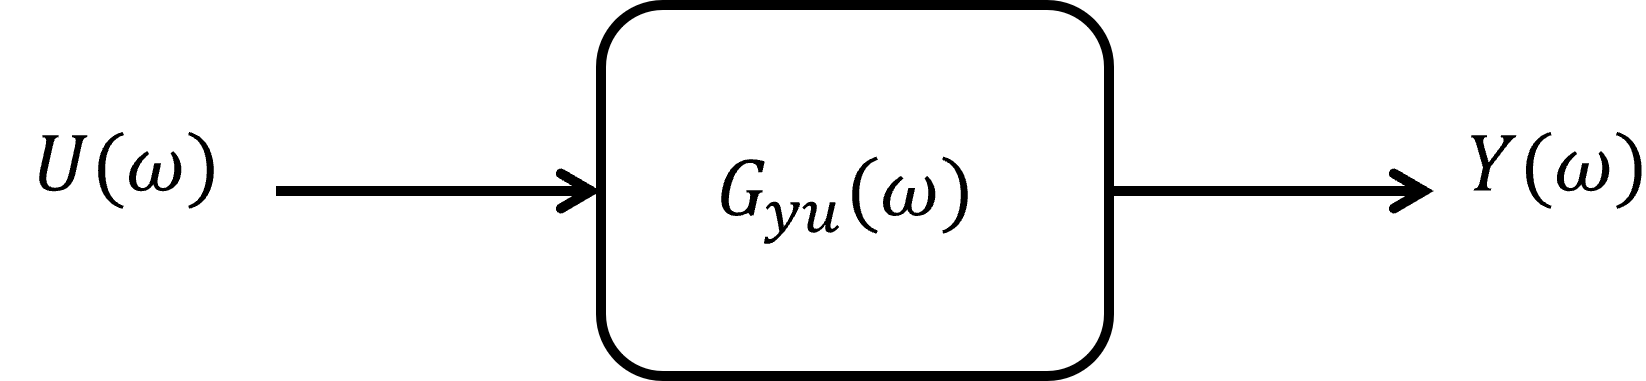
\includegraphics[scale=0.6]{Figuras/UY.png}
\end{figure}

\begin{align*}
    Y(\omega) &= G_{YU}(\omega)U(\omega) \quad \text{(FRF)}\\
    y(t) &= (g_{YU} \ast u)(t) \quad \text{(FRI)}
\end{align*}

Nota: Relación entre FRF y FRI: $G_{YU}(\omega) = \mathcal{F}\{g_{YU}(t)\}$

\subsection{Densidad de poder espectral finita}

\par Recordando el teorema de Wiener-Khinchin, que establece la relación entre \emph{densidad de poder espectral} ($S_{XX}(\Omega)$) y \emph{autocorrelación} ($R_{XX}(\tau)$) de un proceso estocástico w.s.s. $\{X(t),t \in T\}$:

\begin{align*}
    S_{XX}(\Omega) &= \mathcal{F}\{R_{XX}(\tau)\}\\
    R_{XX}(\tau) &= \mathcal{F}^{-1}\{S_{XX}(\Omega)\}
\end{align*}

\noindent donde $R_{XX}(\tau) =\mathbb{E}\{X(t)X(t+\tau)\}$ y $\mathcal{F}\{\cdot\}$ es la transformada de Fourier (contínua).\\

% Ver PSD finito. \parencite[Cap. 5]{Bendat2011}

Mientras, para el caso en tiempo discreto se utiliza la definición de \emph{periodograma}. Suponiendo una muestra finita de $N$ puntos del p.e. $\{X(t),t \in T\}$, con período de muestreo $T_s$:

\begin{align*}
    x[n] =
    \begin{cases}
        x(n T_s), & n\in\{0,1,\ldots,N-1\}\\
        0, & \text{otherwe}
    \end{cases}
\end{align*}

Entonces, el \emph{periodograma} se define como: 

\begin{align*}
    \hat{S}_{XX}(\omega) = \frac{1}{N} X(\omega) X(\omega)^{*} = \frac{1}{N} |X(\omega)|^{2}
\end{align*}

\noindent donde $X(\omega)$ es la transformada de Fourier de tiempo discreto (DTFT) de la señal finita $x[n]$:

\begin{align*}
    X(\omega) = \sum_{n=0}^{N-1} x[n] e^{-j \omega n}
\end{align*}

\noindent y $(\cdot)^{*}$ es la transpuesta conjugada.\\

\emph{Nota:} $S_{XX}(\omega)$ es un valor real.\\

En el límite para $N\to\infty$, el periodograma (un estimador sesgado del PSD) converge al valor real del PSD:

\begin{align*}
    S_{XX}(\omega) = \lim_{N\to\infty} \mathbb{E} \left\{ \hat{S}_{XX}(\omega) \right\}
\end{align*}

Para todo el estudio que viene a continuación consideramos estimaciones de PSD utilizando alguna de las definiciones de periodograma modificado (por ejemplo, método de Welch). %, y para simplificar la notación, utilizaremos ${S}_{XX}(\omega)$ (sin sombrero) como para referirnos a la estimación del PSD de $x(t)$.

\subsection{Relaciones entrada-salida de poder espectral}

Asumir que $u(t)$ e $y(t)$, entrada y salida de un sistema LTI SISO determinístico, son procesos estocásticos w.s.s. de media cero. Entonces, calculemos un estimador del auto PSD de la respuesta $y(t)$:

\begin{align*}
    \hat{S}_{YY}(\omega) &= \frac{1}{N} Y(\omega)Y^{*} (\omega)\\\
    &= \frac{1}{N} \left( G_{YU}(\omega) U(\omega)\right) \left(G_{YU}(\omega) U(\omega)\right)^{*}\\
    &= \frac{1}{N} G_{YU}(\omega) U(\omega) U(\omega)^{*} G_{YU}(\omega)^{*}
\end{align*}

Si el sistema es determinístico, con parámetros sin incertidumbre pero desconocidos:

\begin{align*}
    \hat{S}_{YY}(\omega) &= G_{YU}(\omega) G_{YU}(\omega)^{*} \underbrace{\left\{ \frac{1}{N}U(\omega) U(\omega)^{*} \right\}}_{_{\hat{S}_{UU}(\omega)}}\\
    \hat{S}_{YY}(\omega) &= \left| G_{YU}(\omega) \right|^2 \hat{S}_{UU}(\omega)\\
    \left| G_{YU}(\omega) \right|^2 &= \frac{\hat{S}_{YY}(\omega)}{\hat{S}_{UU}(\omega)}
\end{align*}

\underline{Nota}: $|G_{YU}(\omega)|^2$ es una función real y nos entrega sólo información de la magnitud del sistema y no de la fase. Por lo tanto, \underline{este método queda descartado}.

\subsection{Método \texorpdfstring{$H_1$}{H1}}

Continuando el estudio del sistema SISO LTI:

\begin{align*}
    Y(\omega) &= G_{YU}(\omega)U(\omega) \quad / \cdot U^{*}(\omega)\\
    Y(\omega)U^{*}(\omega) &= G_{YU}(\omega)U(\omega)U^{*}(\omega) \quad / \frac{1}{N} \cdot \\
    \underbrace{\left\{\frac{1}{N}Y(\omega)U^{*}(\omega)\right\}}_{\hat{S}_{YU}(\omega)} &= G_{YU}(\omega)  \underbrace{\left\{\frac{1}{N} U(\omega)U^{*}(\omega) \right\}}_{\hat{S}_{UU}(\omega)} \\
    \hat{S}_{YU}(\omega) &= G_{YU}(\omega) \hat{S}_{UU}(\omega)\\
    \hat{G}_{YU}(\omega) &= \frac{\hat{S}_{YU}(\omega)}{\hat{S}_{UU}(\omega)} \quad \text{(Estimador $H_1$)}
\end{align*}

donde $\hat{S}_{YU}(\omega)$ es la estimación del PSD cruzado entre respuesta $y(t)$ y entrada $u(t)$.\\

\emph{Nota 1:} $\hat{S}_{YU}(\omega)$ es un número complejo.

\emph{Nota 2:} $\hat{G}_{YU}(\omega)$ es un número complejo. Por lo tanto, este método arroja una estimación de la magnitud  $|\hat{G}_{YU}(\omega)|$ y fase $\angle G_{YU}(\omega)$ del sistema dinámico.

\subsection{Método \texorpdfstring{$H_2$}{H2}}

Otra alternativa es el método $H_2$:

\begin{align*}
    Y(\omega) &= G_{YU}(\omega)U(\omega) \quad / \cdot Y^{*}(\omega)\\
    Y(\omega) Y^{*}(\omega) &= G_{YU}(\omega )U(\omega) Y^{*}(\omega) \quad / \frac{1}{N} \cdot \\
    \underbrace{\left\{\frac{1}{N}Y(\omega)Y^{*}(\omega)\right\}}_{\hat{S}_{YY}(\omega)} &= G_{YU}(\omega)  \underbrace{\left\{\frac{1}{N} Y(\omega)U^{*}(\omega) \right\}}_{\hat{S}_{YU}(\omega)} \\
    \hat{S}_{YY}(\omega) &= G_{YU}(\omega) \hat{S}_{YU}(\omega)\\
    \hat{G}_{YU}(\omega) &= \frac{\hat{S}_{YY}(\omega)}{\hat{S}_{YU}(\omega)} \quad \text{(Estimador $H_2$)}
\end{align*}

\subsection{Método \texorpdfstring{$H_v$}{Hv}}

Otra alternativa es el método $H_v$:

\begin{equation*}
    H_v(\omega) =\Re\{H_v(\omega)\} + j\Im\{H_v(\omega)\}
\end{equation*}

que consiste en la media geométrica de estimadores $H_1$ y $H_2$. En este sentido, la media geométrica se toma para cada parte real e imaginaria del FRF por separado:

\begin{align*}
    \Re\{H_v(\omega)\} & = \sqrt{\Re\{H_1(\omega)\} \Re\{H_2(\omega)\}} \\
    \Im\{H_v(\omega)\} & = \sqrt{\Im\{H_1(\omega)\} \Im\{H_2(\omega)\}}
\end{align*}

\subsection{Mediciones con ruido}

% URL: https://dsp.stackexchange.com/questions/71811/understanding-the-h1-and-h2-estimators

En ausencia de ruido en $u(t)$ y $y(t)$, ambos estimadores $H_1$ y $H_2$ coinciden (caso ideal). Pero, en la situación con ruido en las mediciones de entrada y/o salida, hay diferencias relevantes a considerar.

\begin{figure}[H]
    \centering
    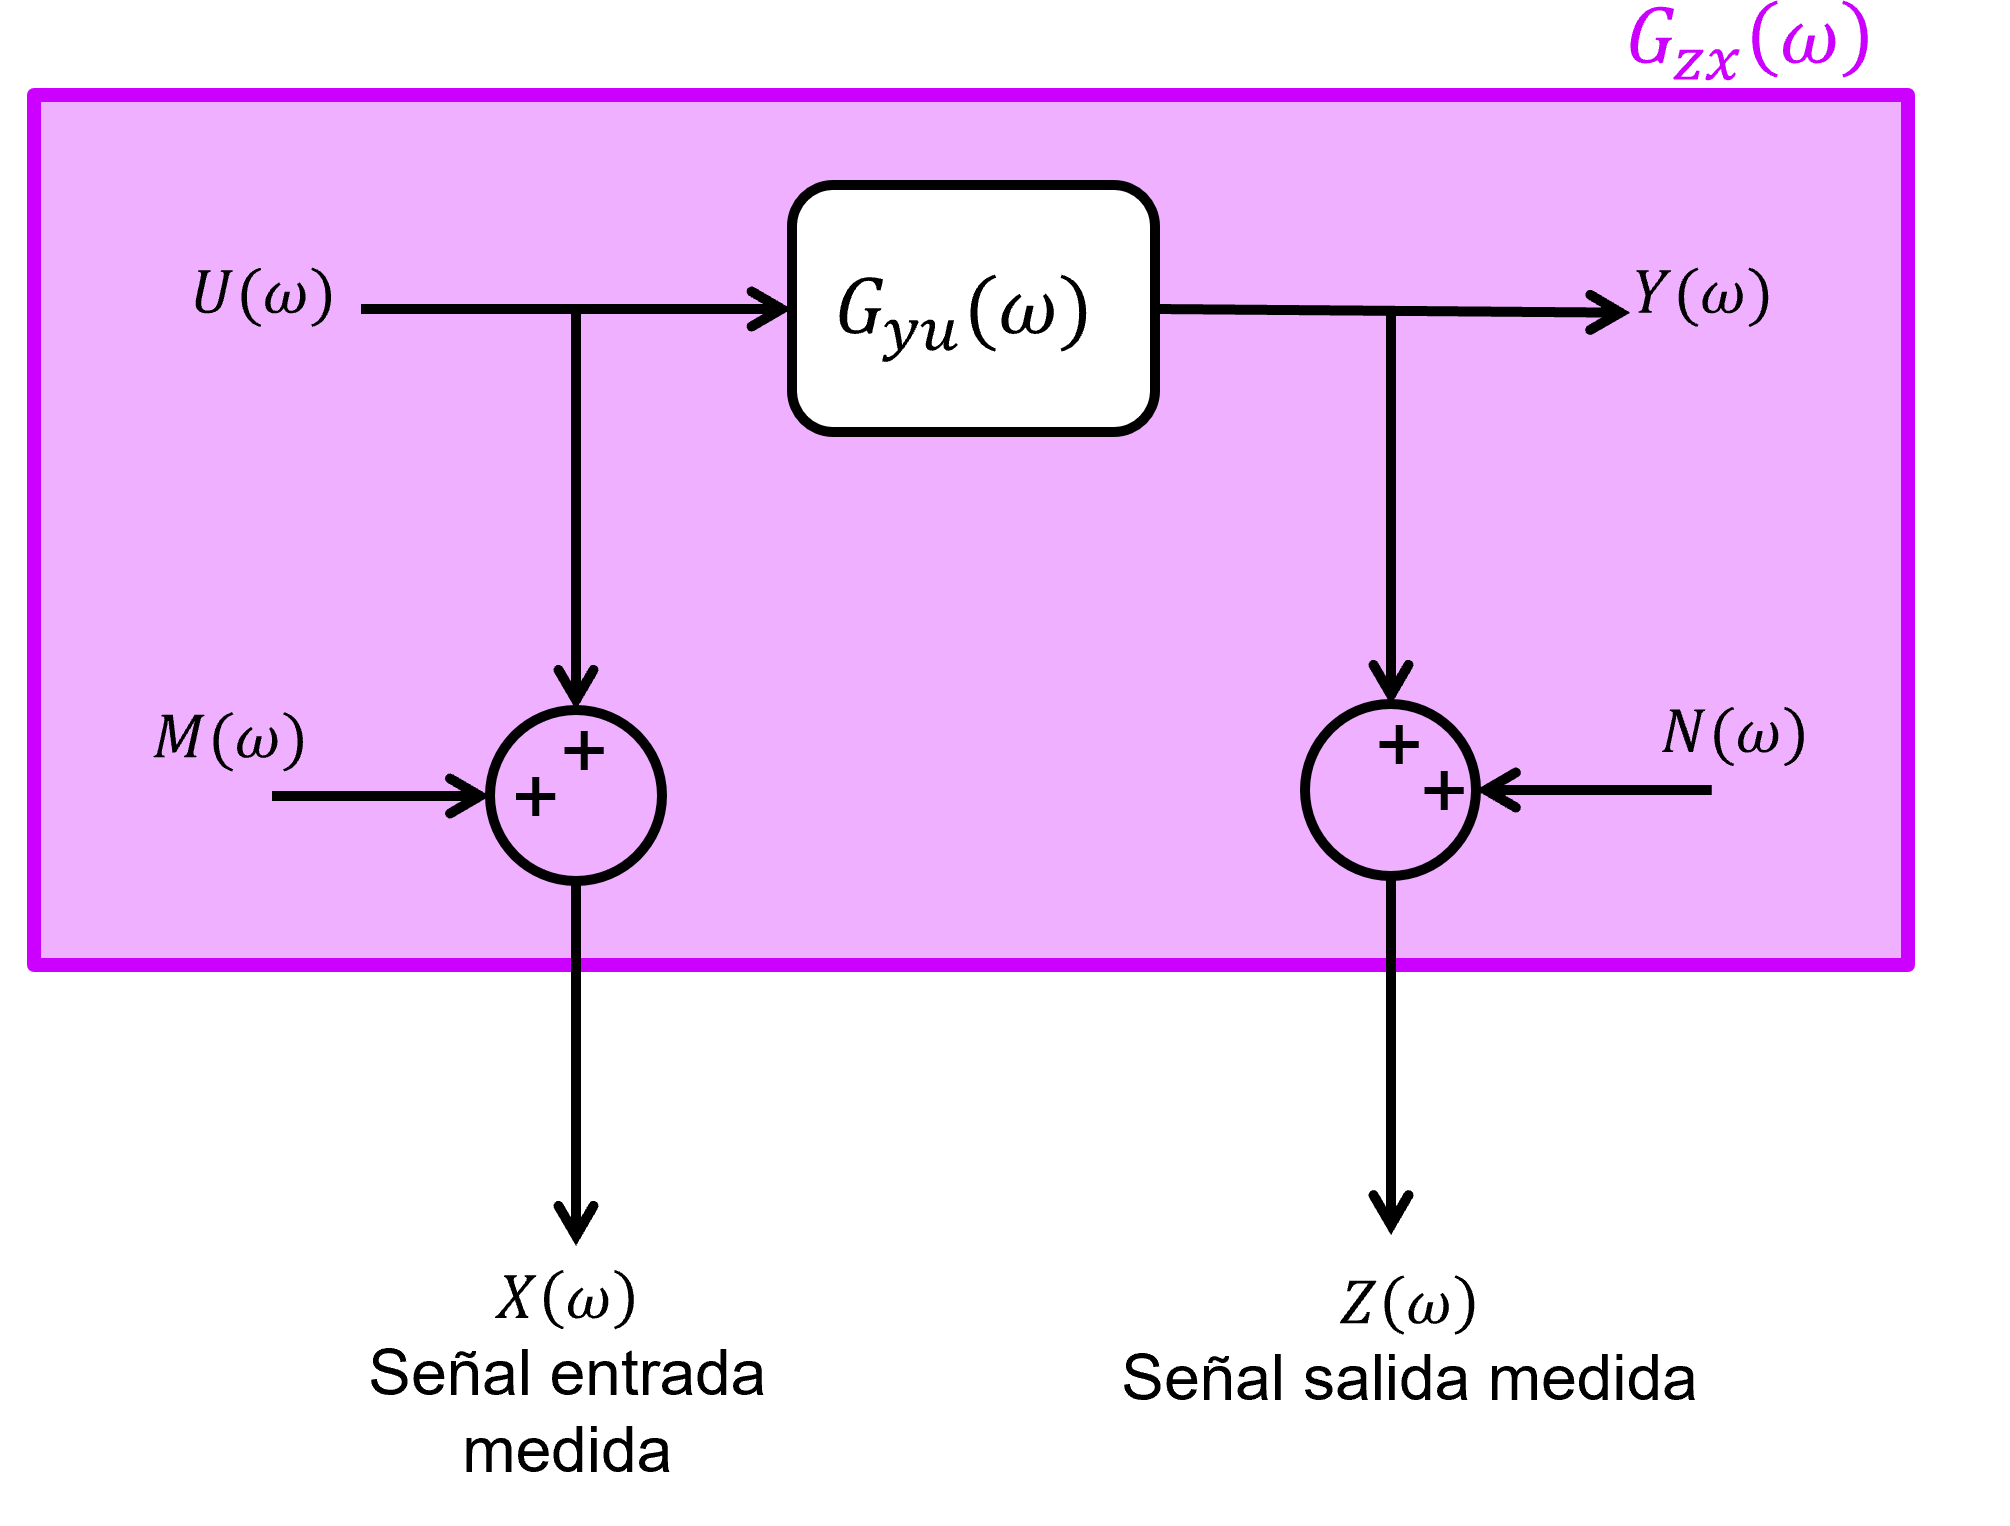
\includegraphics[scale=0.7]{Figuras/H1_ruido.png}
\end{figure}

\par \underline{Nota}: 

\begin{itemize}
    \item Ruido $m(t)$ y $n(t)$ son p.e. estacionarios no correlacionados $\Longrightarrow R_{MN}(\tau) = \mathbb{E}\{m(t) u(t+\tau)\}=0$
    \item Ruido $m(t)$ y entrada $u(t)$ descorrelacionados entre si $\Longrightarrow R_{MU}(\tau) = \mathbb{E}\{m(t) u(t+\tau)\}=0$
    \item Ruido $n(t)$ y salida $y(t)$ descorrelacionados entre si $\Longrightarrow R_{NY}(\tau) = \mathbb{E}\{n(t) y(t+\tau)\}=0$
\end{itemize}

Calculando el auto PSD de señal de entrada medida:

\begin{align*}
    X(\omega) &= U(\omega)+M(\omega)\\
    X(\omega)X^{*}(\omega) &= \left[ U(\omega)+M(\omega)\right] \left[ U(\omega)+M(\omega)\right]^{*}\\
    X(\omega)X^{*}(\omega) &= U(\omega)U^{*}(\omega) + U(\omega)M^{*}(\omega) +  M(\omega)U^{*}(\omega)+ M(\omega)M^{*}(\omega) \quad / \frac{1}{N} \cdot\\
    \hat{S}_{XX}(\omega) &= \hat{S}_{UU}(\omega) + \cancelto{0}{\hat{S}_{UM}(\omega)} + \cancelto{0}{\hat{S}_{MU}(\omega)} + \hat{S}_{MM}(\omega)\\
    \hat{S}_{XX}(\omega) &= \hat{S}_{UU}(\omega)+\hat{S}_{MM}(\omega)
\end{align*}

De forma similar, el auto PSD de señal de respuesta medida:

\begin{align*}
    % Z(\omega) &= Y(\omega)+N(\omega)\\
    \hat{S}_{ZZ}(\omega) &= \hat{S}_{YY}(\omega) + \hat{S}_{NN}(\omega)
\end{align*}

donde:

\begin{align*}
    \hat{S}_{YY}(\omega) = |G_{yu}(\omega)|^2 \hat{S}_{UU}(\omega) 
\end{align*}

Por otra parte, el PSD cruzado de señal de respuesta y entrada medidas:

\begin{align*}
    Z(\omega)X^{*}(\omega) &= \bigl[ Y(\omega)+N(\omega) \bigr] \bigl[ U(\omega)+M(\omega)\bigr]^{*}\\
    Z(\omega)X^{*}(\omega) &= Y(\omega)U^{*}(\omega)+Y(\omega)M^{*}(\omega)+N(\omega)U^{*}(\omega)+N(\omega)M(\omega)^{*} \quad / \frac{1}{N}\cdot \\
    \hat{S}_{ZX}(\omega) &= \hat{S}_{YU}(\omega) + \cancelto{0}{\hat{S}_{YM}(\omega)} + \cancelto{0}{\hat{S}_{NU}(\omega)} + \cancelto{0}{\hat{S}_{NM}(\omega)}\\
    \hat{S}_{ZX}(\omega) &= \hat{S}_{YU}(\omega)
\end{align*}

Entonces, el estimador $H_1$: 

% \begin{align*}
%     Z(\omega) &= G_{ZX}(\omega)(\omega)\\
%     Z(\omega)X^{*}(\omega) &= G_{ZX}(\omega)X(\omega)X^{*}(\omega)\\
%     \hat{S}_{ZX}(\omega) &= G_{ZX}(\omega)\hat{S}_{XX}(\omega)
% \end{align*}

\begin{align*}
    \hat{G}_{ZX}(\omega) &= \frac{\hat{S}_{ZX}(\omega)}{\hat{S}_{XX}(\omega)}=\frac{\hat{S}_{YU}(\omega)}{\hat{S}_{UU}(\omega)+\hat{S}_{MM}(\omega)}\\
    &= \frac{\hat{S}_{YU}(\omega)/\hat{S}_{UU}(\omega)}{1+\hat{S}_{MM}(\omega)/\hat{S}_{UU}(\omega)}\\
    &= \frac{G_{YU}(\omega)}{1+\hat{S}_{MM}(\omega)/\hat{S}_{UU}(\omega)} \\
    &= G_{YU}(\omega) \underbrace{\left[ \frac{1}{1+\hat{S}_{MM}(\omega)/\hat{S}_{UU}(\omega)} \right]}_{< 1} < G_{YU}(\omega)
\end{align*}

donde el término $\hat{S}_{MM}(\omega)/\hat{S}_{UU}(\omega)$ es el efecto del ruido de entrada $M(\omega)$. Luego, $H_1$ es un limite inferior de $G_{YU}(\omega)$.\\

\par De manera similar, el estimados $H_2$:

\begin{align*}
    \hat{G}_{ZX}(\omega) &= \frac{\hat{S}_{ZZ}(\omega)}{\hat{S}_{ZX}(\omega)}\\
    &= G_{YU}(\omega) \underbrace{\left[1 +\frac{\hat{S}_{NN}(\omega)}{\hat{S}_{YY}(\omega)}\right]}_{> 1} > G_{YU}(\omega)
\end{align*}

donde el término $\hat{S}_{NN}(\omega)/\hat{S}_{YY}(\omega)$ es el efecto del ruido de salida. Luego, $H_2$ es un límite superior de $G_{YU}(\omega)$

\subsection{Función de coherencia}

La función de coherencia ordinaria es una herramienta que mide que tanto de la señal de salida se explica (o relaciona) con la señal de entrada. Puede ser utilizado como un indicador de calidad del estimador H1/H2.

\begin{align*}
    \gamma_{ZX}^2(\omega) = \frac{|\hat{S}_{ZX}(\omega)|^2}{\hat{S}_{ZZ}(\omega)\hat{S}_{XX}(\omega)} = \frac{H_1(\omega)}{H_2(\omega)}
\end{align*}

donde $ 0 < \gamma_{ZX}^2 < 1$.\\

\emph{Notas}:

\begin{enumerate}
    \item Si $\gamma_{ZX}^2 \approx 1$, entonces existe buena coherencia entre entrada y salida. En general, los peaks de resonancia deben tener un valor de coherecia cercano a 1.
    \item Si $\gamma_{ZX}^2 \approx 0$, no existe correlación entre entrada y salida del sistema. Esto ocurre especialmente en anti-resonancias, donde la estructura rechaza la entrada en la frecuencia correspondiente.
    \item Si la coherencia es baja (por ejemplo, $\gamma_{ZX}^2 << 1$), puede deberse a problemas asociados con el experimento. Por ejemplo,  ruido de medición es excesivo, entrada no excita adecuadamente la estructura, o problemas de \emph{spectral leakage} por uso inapropiado de ventanas del periodograma modificado.
    \item Si la coherencia es baja cerca de los peaks de resonancia, puede ocurrir que el sistema sea nolineal, en cuyo caso se requiere de otros métodos avanzados de identificación.
\end{enumerate}


% \par Análogo a regresión lineal:

% \begin{align*}
%     Z=\theta X+\varepsilon
% \end{align*}

\subsection{Procedimiento}

\begin{enumerate}

    \item Instalar sensores en el sistema a identificar.

           \underline{Nota}: Debe satisfacer la condición de observabilidad
    
        % \begin{figure}[H]
        %     \centering
        %     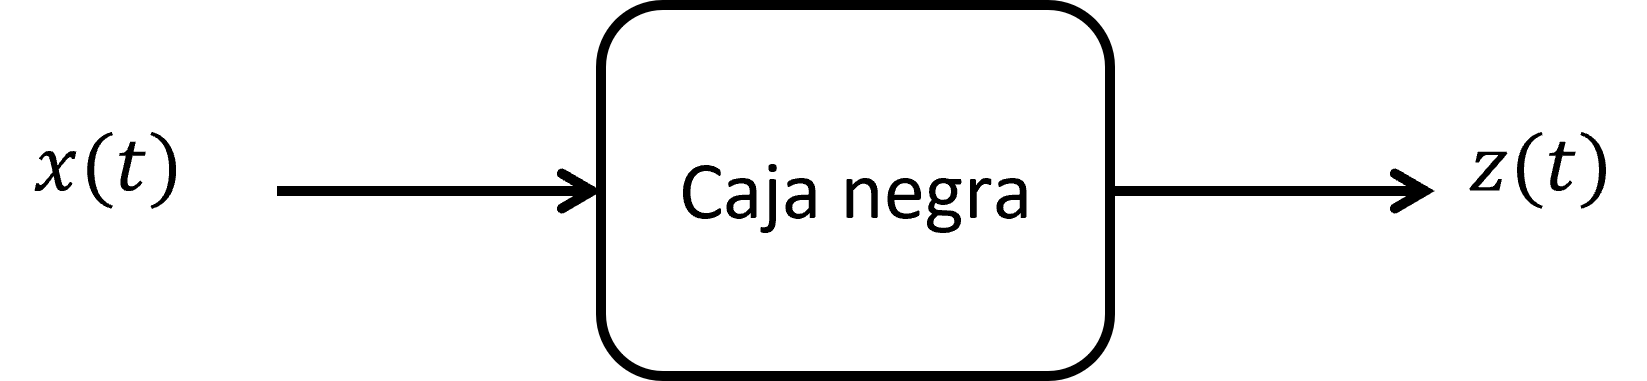
\includegraphics[scale=0.7]{Figuras/caja_negra.png}
        % \end{figure}
        
    \item Generar un ruido blanco de entrada. \emph{Nota:} La entrada debe ser una excitación persistente, es decir, la señal debe ser rica en un amplio espectro de frecuencias (suficientes armónicas).
    
    \item Medir $x[n]$ y $z[n]$.

    \item Realizar postprocesamiento a las señales de medición (detrend, resampling, etc.).
    
    \item Estimar $H_{true}(\omega) = G_{YU}(\omega)$ utilizando $H_1$ o $H_2$.\\

    \emph{Nota:} $|H_1(\omega)| \leq |H_{true}(\omega)| \leq |H_2(\omega)|$

    \item Calcular $\gamma_{ZX}^2$ y revisar la calidad de la estimación FRF.
    
        % \begin{figure}[H]
        %     \centering
        %     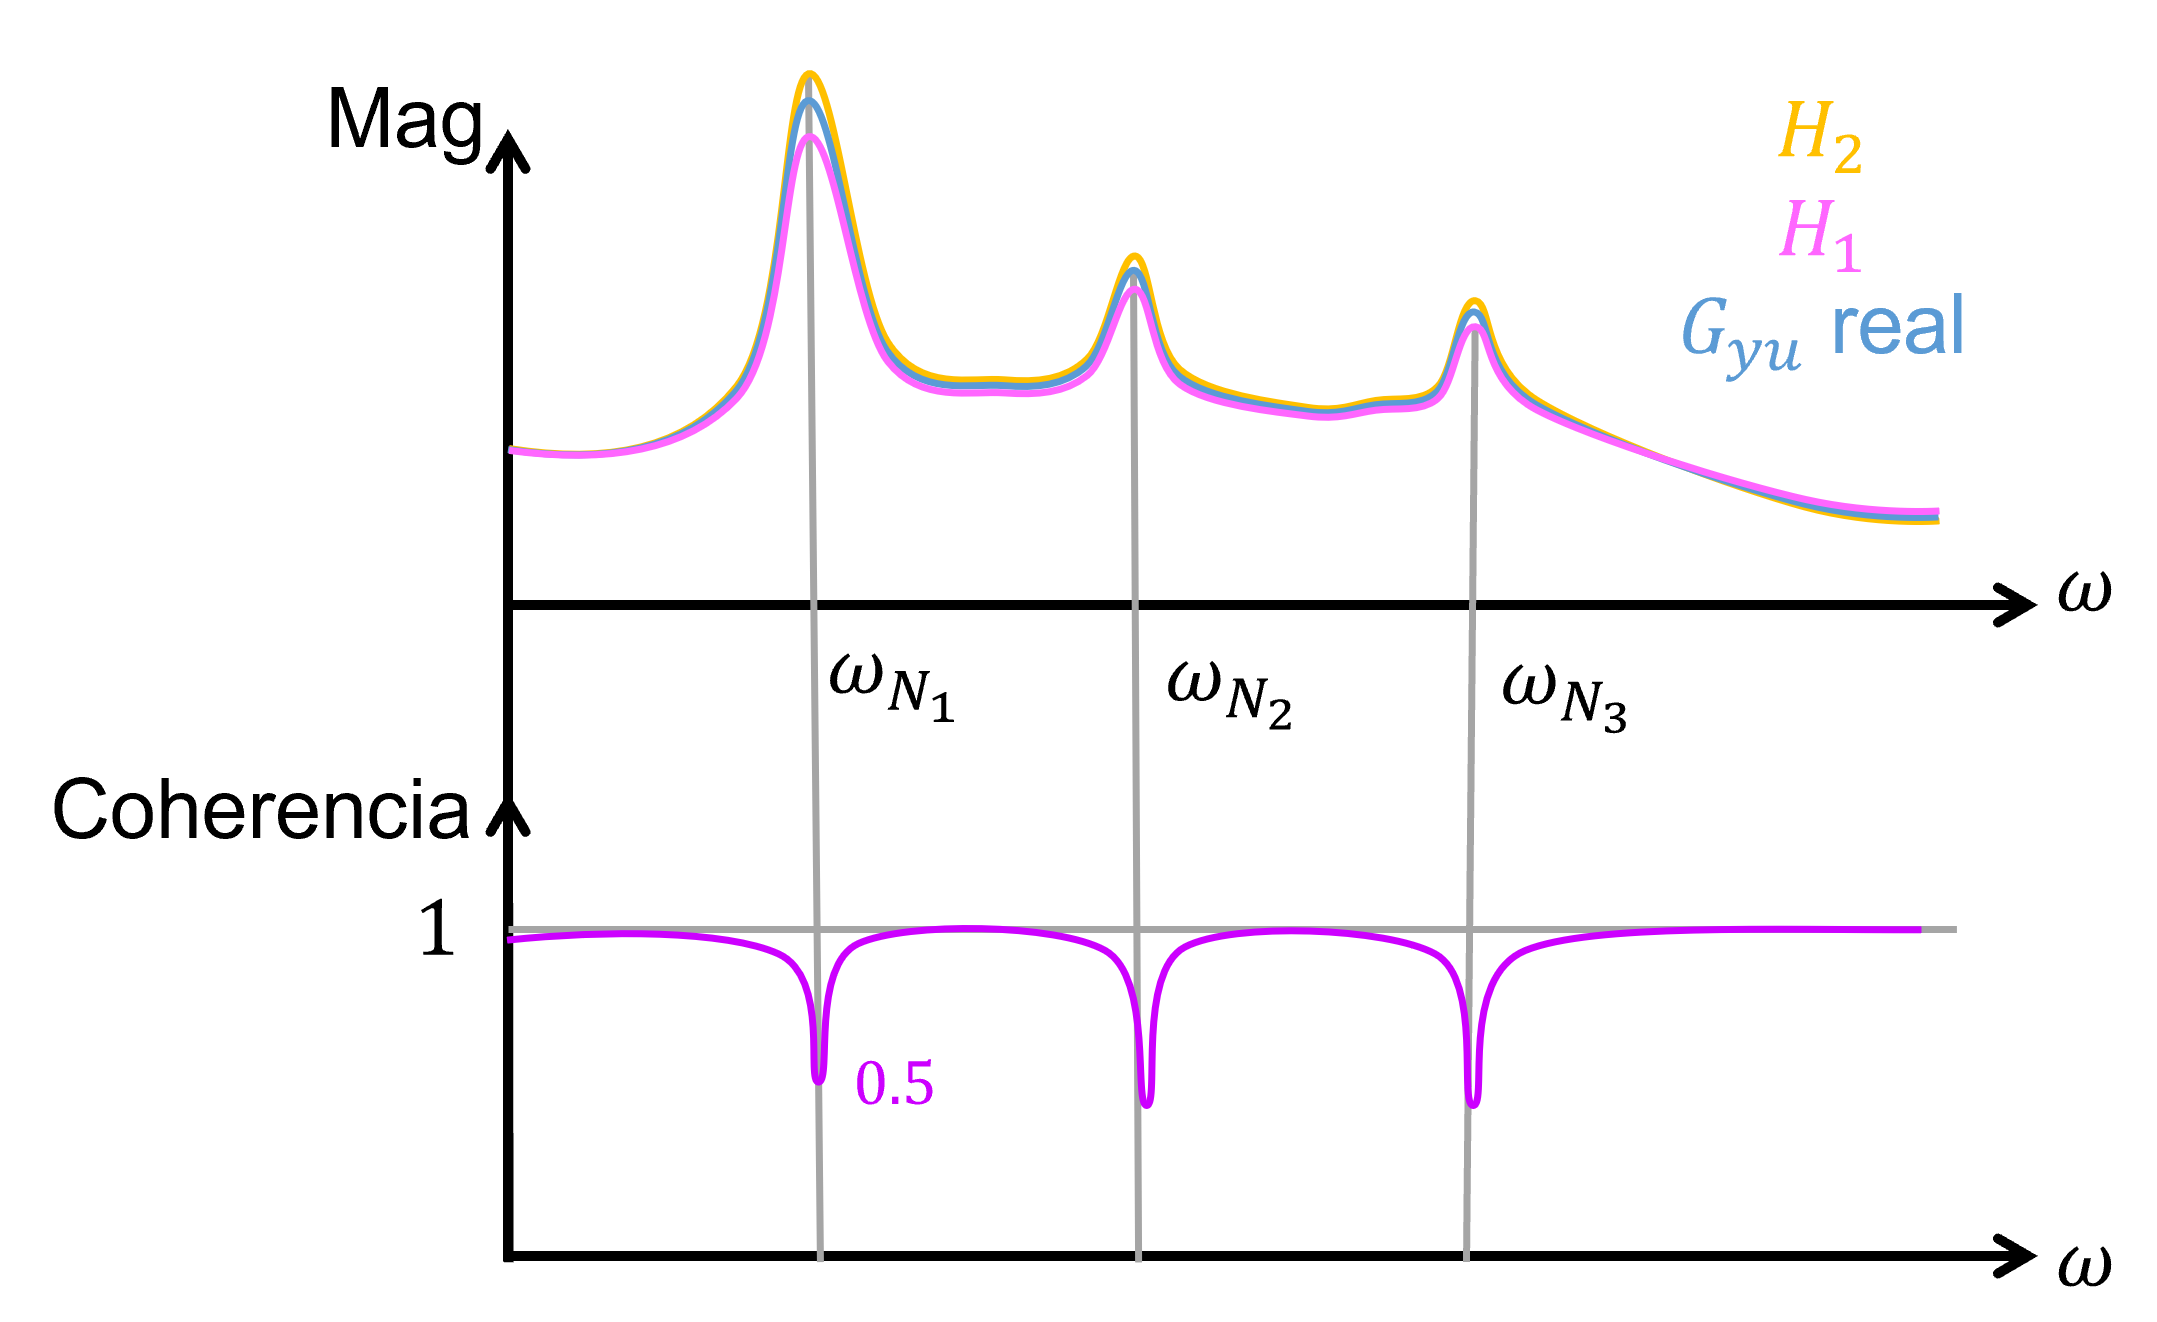
\includegraphics[scale=0.7]{Figuras/Gyu.png}
        % \end{figure}
        
\end{enumerate}

% En estricto rigor, $H_1$ y $H_2$ nos entregan una respuesta discretizada para valores de $\omega \in \{\omega_0,\omega_1,...,\omega_N\}$\\

En \emph{Matlab}, la función \texttt{tfestimate()} determina el FRF experimental con estimadores H1/H2, donde los periodogramas se determinan usando el método de Welch. Link:
\url{https://www.mathworks.com/help/signal/ref/tfestimate.html}.

% Otras alternativas son \texttt{etfe()} y \texttt{spa()}.

\subsection{Frecuencias y formas modales utilizando \emph{peak-picking}}

Referencia: \textcite[Sec. 18.6]{craig2006fundamentalsstructural}

Considere la EDM de un sistema MDOF:

\begin{equation}
    M \ddot{u} + C \dot{u} + K u = G p(t)
\end{equation}

\noindent donde $u(t) \in \mathbb{R}^n$ y $p(t) \in \mathbb{R}$ son los GLs y la excitación, respectivamente; $M \in \mathbb{R}^{n \times n}$, $C \in \mathbb{R}^{n \times n}$ y $K \in \mathbb{R}^{n \times n}$ son las matrices de masa, amortiguamiento y rigidez, respectivamente; $G \in \mathbb{R}^{n}$ es el vector de participación de la excitación $p(t)$ en la dinámica del sistema.

De la solución del problema de valores y vectores propios generalizados:

\begin{equation}
    K \phi = \lambda M \phi
\end{equation}

\noindent donde $\lambda_r = \omega_r^2$ y $\phi_r$ es el valor y vector propio del modo $r$. De este resultado podemos definir coordenadas modales  en notación matricial:

\begin{equation}
    u(t) = \Phi q(t)
\end{equation}

\noindent donde $\Phi = [\phi_1, \phi_2, \ldots,\phi_n]$ es la matriz de formas modales del sistema.

La relación entre coordenadas físicas y modales la podemos describir en notación indicial:

\begin{equation}\label{eq:coordmod}
    u_{s}(t) = \phi_{sr} q_r(t)    
\end{equation}

Asumiendo amortiguamiento proporcional, la EDM de la coordenada modal $q_r(t)$ se escribe:

\begin{equation}
    \ddot{q}_{r} + 2 \zeta_r \omega_r \dot{q}_{r}  + \omega_r^2 q_r = \underbrace{\phi_{kr} G_k}_{\gamma_r} p(t)
\end{equation}

Aplicando la transformada de Fourier, podemos calcular el FRF de la coordenada modal $q_r$ dada la entrada $p$:

\begin{equation}
    H_{q_{r} p}(\Omega) = \frac{\gamma_r}{(\omega_r^2 - \Omega^2) + j (2 \zeta_r \omega_r \Omega)}
\end{equation}

Volviendo a \eqref{eq:coordmod}, aplicando la transformada de Fourier:

\begin{align}
    U_{s}(\Omega) &= \phi_{sr} Q_r(\Omega) \\
                  &= \phi_{sr} H_{q_rp}(\Omega) P(\Omega) \\
                  &= H_{u_{s} p}(\Omega) P(\Omega)
\end{align}

Por lo tanto:

\begin{equation}
    H_{u_{s} p}(\Omega) = \frac{\gamma_r}{(\omega_r^2 - \Omega^2) + j (2 \zeta_r \omega_r \Omega)} \phi_{sr}
\end{equation}

Notar que cuando $\Omega = \omega_r$, el FRF tiene solo parte imaginaria:

\begin{equation}
    H_{u_{s} p}(\omega_r) = \frac{\gamma_r}{j (2 \zeta_r \omega_r^2)} \phi_{sr}
\end{equation}

Entonces, el peak ``r'' de la parte imaginaria de $H_{u_{s} p}$ es proporcional a la componente $\phi_{sr}$ de la forma modal $r$:

\begin{equation}
    \Im\left\{H_{u_{s} p}(\omega_r)\right\} \propto \phi_{sr}
\end{equation}

Podemos ocupar esta información para estimar las formas modales utilizando FRF experimentales:

\begin{figure}
    \centering
    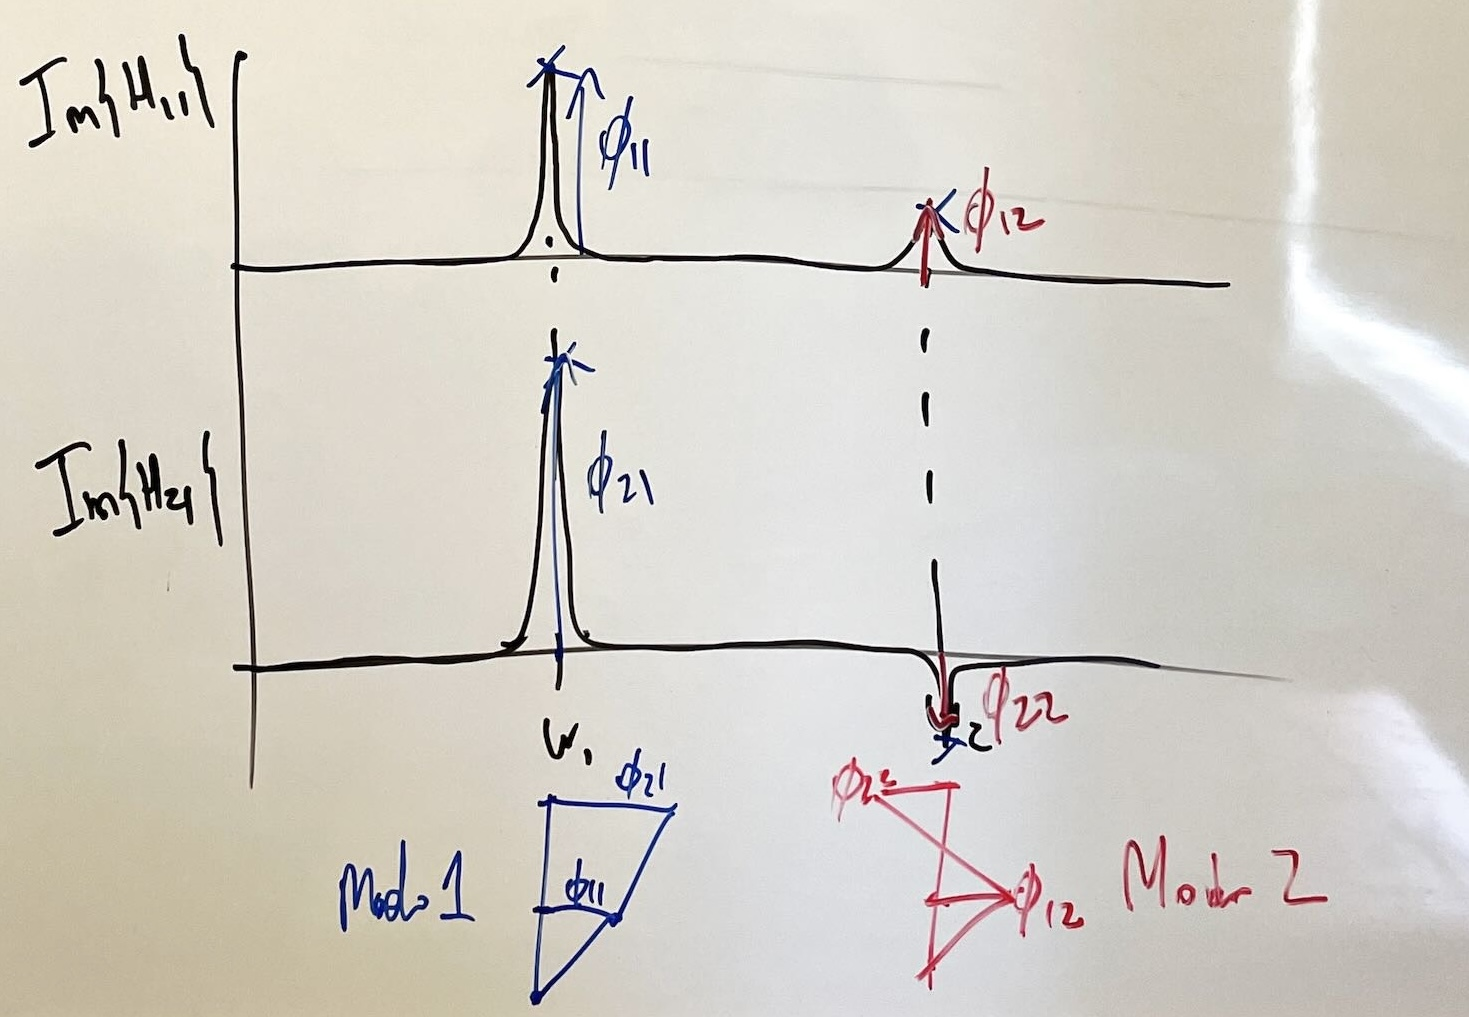
\includegraphics[width=6in]{Figuras/expmodeshapes.JPG}
    \caption{Estimación de formas modales}
\end{figure}

\subsection{Ajuste de modelos no paramétricos}

Métodos de estimación de parámetros \parencite[Cap. 7]{Ljung1998}:

\begin{itemize}
    \item Least squares (LS)
    \item Prediction-error methods (PEM)
    \item Maximum likelihood estimator (MLE)
    \item Instrumental Variable (IV)
\end{itemize}

System Identification Toolbox de Matlab. URL: \url{https://www.mathworks.com/help/ident/index.html}.

\section{Métodos de identificación \emph{ouput-only} }

En algunos casos no se conoce la entrada que actúa sobre el sistema estructural. En esas situaciones, la identificación del sistema se realiza solo a partir de las respuestas medidas (\emph{output-only}), como el desplazamiento, la velocidad o la aceleración. Estas respuestas se deben a excitaciones ambientales o de operación. A veces, el procedimiento se conoce como análisis modal operacional (\emph{operational modal analysis}, OMA).

\subsection{Frequency domain decomposition (FDD)}

El método de descomposición en el dominio de la frecuencia (FDD) permite aproximar las frecuencias y modos de vibrar a partir del cálculo de descomposición de valores singulares de la función de PSD \parencite{brincker2001modalidentification}. Los valores singulares se pueden utilizar para definir un sistema SDOF equivalente caracterizado por los mismos parámetros modales que el sistema MDOF que se está investigando.

% Sin embargo, la estimación de los modos de vibrar puede ser sesgada, debido a que la descomposición de valores singulares fuerza a que los vectores sean ortogonales. En caso de que los modos de vibrar sean ortogonales, la estimación no es sesgada.

Algoritmo:

\begin{enumerate}
    \item Medir respuesta multivariada del sistema $y[n] \in \mathbb{R}^{m \times 1}$. Esto quiere decir que se miden $m$ respuestas del sistema dinámico.
    \item Calcular auto PSD de respuesta $S_{yy}(\omega) \in \mathbb{R}^{m \times m}$ utilizando método de Welch.
    \item Descomponer $S_{yy}(\omega_i)$ utilizando SVD:

        \begin{equation}
            S_{yy}(\omega_i) = U_i \Sigma_i U_i^*, \qquad \forall i\in\{0,\ldots,N\}
        \end{equation}

    donde $U_i = [u_{i1}, u_{i2}, \cdots, u_{iN}]$.
    
    \item Graficar valores singular vs frecuencia, e identificar los peaks.
    \item En un peak asociado al modo $k$ (es decir, en frecuencia $\omega_k$), si no hay otros peaks cercanos, y es el peak dominante, entonces la primera columna de $U_k$ corresponde a la forma modal:

        \begin{equation}
            \varphi_k = u_{k1}
        \end{equation}
    
    y los valores singulares vecinos corresponden al auto PSD del sistema SDOF equivalente en coordenadas naturales.
    \item Utilizar indicador MAC (\emph{modal assurance criterion}) para decidir si la forma modal es adecuada. 
\end{enumerate}

\subsection{Enhanced Frequency Domain Decomposition (EFDD)}

El método \emph{Enhanced Frequency Domain Decomposition} (EFDD) es una extensión del método FDD que permite estimar no solo las frecuencias naturales, sino también las razones de amortiguamiento modales del sistema. Este procedimiento consiste en aislar los datos obtenidos mediante la descomposición en valores singulares (SVD) alrededor de un peak del espectro, y transformarlos al dominio del tiempo para obtener una función de correlación. A partir de esta función, se asume un comportamiento de un sistema de un solo grado de libertad (SDOF), lo que permite determinar con mayor precisión las frecuencias naturales y los amortiguamientos, de manera independiente de la resolución espectral y facilitando la identificación de modos cercanos en frecuencia.

%\subsection{Métodos de subespacio}

\subsection{Eigensystem Realization Algorithm (ERA)}

Referencia: \textcite{Juang1985}

Matlab: \texttt{era()}. URL: \url{https://www.mathworks.com/help/ident/ref/era.html}

\subsection{Natural Excitation Technique (NExT)}

El método \emph{Natural Excitation Technique} (NExT) se basa en que, cuando una estructura es excitada por una entrada de tipo ruido blanco, la función de correlación cruzada entre las respuestas medidas en dos puntos distintos es proporcional a la función de respuesta impulsiva (FRI) del sistema. Esto permite obtener la información dinámica de la estructura a partir únicamente de sus respuestas, sin necesidad de conocer la excitación aplicada.

%\subsection{Random Decrement Technique (RDT)}


\subsection{Stochastic Subspace Identification (SSI)}

Referencia: \textcite{vanoverschee2011subspaceidentification}

Clase de algoritmos que utilizan proyecciones (oblícuas) de subespacios y algebra lineal (factorización QR y SVD) para buscar la representación de variables de estado del sistema, $(A, B, C, D)$.

Alternativas para construir matriz Hankel: Data-Driven (SSI-DATA) y Covariance-Driven (SSI-COV).

% What it is: N4SID is the general name for the class of algorithms that use subspace projections (specifically, oblique projections) and linear algebra (like QR factorization and SVD) to find a system's state-space matrices (A, B, C, D).

% Application: It's a broad framework that can be used for both:

% Input-Output (Deterministic) ID: When you have measured both the input (e.g., shaker force) and the output (e.g., acceleration).

% Output-Only (Stochastic) ID: When you only have the output measurements and must assume the input is unknown white noise. When N4SID is used in this context, it is called Stochastic Subspace Identification (SSI).

% In short, SSI-DATA and SSI-COV are two specific types of N4SID adapted for the stochastic (output-only) case.

% 2. SSI-COV vs. SSI-DATA (The "Implementations")

% The fundamental difference between these two SSI methods is what data is used to build the main Block-Hankel matrix (the large matrix that organizes the system's past and future data).

% �� SSI-COV (Covariance-Driven)

% This is a two-step process that uses output covariances.

% Step 1: Calculate Covariances: The algorithm first computes the output covariance functions from the raw time-series data. This step essentially averages the data and acts as a form of data compression.

% Step 2: Build Hankel Matrix: It then constructs the Block-Hankel matrix using these calculated covariance values, not the raw data.

% Solve: The N4SID algorithm (SVD, etc.) is then applied to this covariance-based Hankel matrix to find the state-space model.

% Key Feature: It works with covariance functions. This can be computationally faster for extremely long datasets because the covariance matrix is much smaller than the raw data matrix.

% �� SSI-DATA (Data-Driven)

% This is a one-step process that works directly with the measurements.

% Step 1: Build Hankel Matrix: The algorithm constructs the Block-Hankel matrix directly from the raw time-series data.

% Solve: The N4SID algorithm (often involving an efficient QR factorization first, then SVD) is applied to this massive data matrix to find the state-space model.

% Key Feature: It works directly with raw time-series data. This avoids the intermediate step of calculating covariances (which can sometimes introduce bias) and is often considered more numerically robust.


% MAC: Modal Assurance Criterion

Función Matlab \texttt{n4sid()}. URL: \url{https://www.mathworks.com/help/ident/ref/n4sid.html}.

\part{Tópicos avanzados}

\chapter{Simulación híbrida}

\emph{En desarrollo.}


\chapter{Aprendizaje automático}

\emph{En desarrollo.}

\appendix

\part{Apéndice}

\chapter{Introducción a Matlab}
\section{Introducción}
\textbf{MATLAB} (\textbf{MAT}rix \textbf{LAB}oratory) es un entorno y lenguaje de programación. Su ventaja es su capacidad para realizar operaciones de arreglos multidimensionales como vectores ($n \times 1$), matrices ($n \times m$), etc. de manera rápida y sencilla. \\

\noindent MATLAB tiene documentación para todas sus funciones. Dentro del mismo entorno se puede consultar cómo utilizar una función escribiendo \emph{help nombre\_función} en la ventana de comandos o consultando su página web, la cual contiene ejemplos:

\section{Crear Variables}
Las variables se utilizan para almacenar datos. Hay diversas estructuras de datos para almacenarlos, como escalares, vectores, matrices, también, cadenas de texto (string), celdas (cells), estructuras (struct) a las que se les asignan letras o variables:

\subsection{Crear arreglos}
Un arreglo es un escalar, vector, matriz, etc. Con dimensiones $m \times n \times o \times p \times ...$ \\

Ej: Crear las siguientes variables: $a = 1$, $b = \begin{bmatrix}
1 \\
2 \\
3
\end{bmatrix}
$ y $c = \begin{bmatrix}
1 & 2 & 3 \\
4 & 5 & 6 \\
7 & 8 & 9
\end{bmatrix}
$

\begin{verbatimg}
    a = 1;                          % número escalar (o arreglo de 1 dimensión)
    b = [1; 2; 3];                  % vector de números (o arreglo 3x1)
    c = [1 2 3; 4 5 6; 7 8 9];      % matriz de números (o arreglo 3x3)
\end{verbatimg}

\noindent Los comentarios van con signo de porcentaje \%. Para no mostrar la asignación de la variable en la ventana de comandos, escribir ; al final de la asignación.

\subsubsection{Inicializar arreglos}
Es una buena practica primero inicializar un vector/matriz vacío (llenos de ceros o unos) ya que MATLAB primero asigna un espacio en la memoria, por lo que si se desea añadir un nuevo elemento al arreglo, se tendría que reasignar el espacio en la memoria todas las veces que se modifica.
\begin{verbatimg}
    A = zeros(3,4); % Inicializar matriz con ceros, 3 filas y 4 columnas
    v = zeros(3,1); % Inicializar vector con ceros, 3 filas
    A = ones(5,5);  % Inicializar vector con unos, 5 filas y 5 columnas
\end{verbatimg}

\subsubsection{Vectores desde rango}
Ej: Vector de tiempos para una simulación:
\begin{verbatimg}
    t_inicio = 0; % s
    t_final = 10; % s
    paso_tiempo = 0.1; % s
    t = (t_inicio:paso_tiempo:t_final); % vector fila
\end{verbatimg}

\subsubsection{Recorrer arreglos}
\noindent Para observar qué contiene un arreglo (vector o matriz) en una posición específica:

\begin{itemize}
    \item \emph{matriz(i, j)} para ver el elemento en fila i, columna j
    \item \emph{matriz(i, :)}  para ver la fila i (todas las columnas), vector fila
    \item \emph{matriz(:, j)}  para ver columna j (todas las filas), vector columna
    \item \emph{matriz(:, :)}  toda la matriz
    \item \emph{matriz(i:e, j:k)} para ver matriz entre las filas i y e y las columnas j y k
    \item \emph{vector(j: end)} para ver elemetos en vector desde la fila j en adelante.
    \item \emph{arreglo(i, j, k)} para ver la matriz k en la fila i columna j (se puede ver como un vector de matrices)
\end{itemize}

\subsubsection{Filtrar arreglos}
\begin{verbatimg}
    vector = [1; 0; 2; 0; 3; 4; 0; 5; 0];
    filtro_1 = vector(vector != 0) % tomar todo lo que no es 0, esto retorna filtro_1 = [1; 2; 3; 4; 5]
    filtro_2 = vector(vector == 1) % toma todo lo que es 1, esto es [1]
\end{verbatimg}

\subsubsection{Eliminar elementos}
\begin{verbatimg}
    v(5) = [ ];     % Borrar quinto elemento de un vector
    M(5, :) = [ ];  % Borrar la quinta fila de una matriz
\end{verbatimg}

\subsection{Números complejos}
\begin{verbatimg}
    num_complejo = 1 + 3i;  % crear numero complejo
    real(num_complejo)      % parte real del NC, retorna 1
    imag(num_complejo)      % parte imaginaria del NC, retorna 3
\end{verbatimg}

\subsection{Variables simbólicas}
Si se desea trabajar con expresiones algebraicas se pueden crear \emph{variables simbólicas}. No es recomendable trabajar con variables simbólicas ya que MATLAB es ineficiente para trabajar con este tipo de variables:

\begin{verbatimg}
    syms t          % crear variable 't' (t es una variable tipo simbólica)
    x = 1 + 3*t;    % x es una variable tipo simbólica
\end{verbatimg}

\subsection{Serie de caracteres}
Las series de caracteres se dividen en \emph{strings} y \emph{chars}, cada una tiene sus propias funciones para operar con ellas:
\begin{verbatimg}
    caracteres = 'abcdfghijk';      % char
    caracteres_2 = "qwertyuiop";    % string
\end{verbatimg}

\subsection{Structs}
Para almacenar diferentes tipos de datos en una misma variable, se puede utilizar un \emph{struct} (similar a diccionarios en python):\\

Ej: Para 10 registros sísmicos, guardar los vectores de aceleración del registro, tiempo del registro, aceleración espectral, periodos de la aceleración espectral, duración del registro. 
\begin{verbatimg}
    n_registros = 10;
    dataRegistros = struct()                % inicializar un struct    
    for i =  1:n_registros                  % para cada registro...
        [reg, t] = importReg(registro(i));  % Suponga tenemos función para importar registros
        % Guardar datos en struct
        dataRegistros(i).registro = reg;
        dataRegistros(i).tiempo = t;
        dataRegistros(i).Sa = computeSa(reg, t, T, xi);
        dataRegistros(i).duracion = max(t); % o t(end)
    end
    %  Entonces, para consultar sobre el tiempo del tercer registro
    vector_tiempo_3er_registro = dataRegistro(3).tiempo;
\end{verbatimg}

\noindent Los \emph{structs} organizan y estructuran datos de manera coherente en el código y se utilizan especialmente para simplificar las funciones al reducir la cantidad de inputs necesarios. En lugar de escribir múltiples inputs, se utiliza solo uno que luego se descompone dentro de la función.

\section{Operaciones}
Para saber que tipo de variable es una variable, comando \emph{class()}
\begin{verbatimg}
    A = [1;2;3];
    class(A)  % retorna 'A is double'
\end{verbatimg}

\subsection{Operaciones Básicas}
Las operaciones funcionan igual que las operaciones matriciales y vectoriales. \\

Sumar arreglos (matlab suma componentes (i,j) de cada arreglo)
\begin{verbatimg}
    suma_matrices = matriz_1 + matriz_2;
\end{verbatimg}

Sumar elementos del arreglo
\begin{verbatimg}
    suma_vector = sum(vector_1)
\end{verbatimg}

Restar (matlab resta componentes (i,j) de cada arreglo)
\begin{verbatimg}
    resta_matrices = matriz_1 - matriz_2;
\end{verbatimg}

Multiplicar
\begin{verbatimg}
    matriz_por_matriz = matriz_1*matriz_2;
    vector_por_vector_componente = vector_1.*vector_2;
\end{verbatimg}

Invertir matrices $matriz^{-1}$
\begin{verbatimg}
    matriz_invertida = matriz_1^-1; % o inv(matriz)
\end{verbatimg}

Trasponer matrices $matriz^T$
\begin{verbatimg}
    matriz_traspuesta = matriz_1.';
\end{verbatimg}

Diferenciar e integrar
\begin{verbatimg}
    vector_diferenciado = diff(vector_1);
\end{verbatimg} 

Suma acumulada
\begin{verbatimg}
    vector_suma_acumulada = cumsum(vector_1);
\end{verbatimg}

\noindent Además, MATLAB también incluye las funciones de operaciones matemáticas básicas
\begin{itemize}
    \item log() y exp() - Logaritmo natural y exponencial
    \item sqrt() y ()\^x - Raíces y Potencias
    \item sin() y cos() - Seno y coseno
    \item $X = A\setminus B$ - Solución de $A*X = B$
    \item $X = B/A$ - Solución de $X*A = B$
    \item diag() - de vector a matriz diagonal o extraer diagonal de una matriz
\end{itemize}

\subsection{Función por partes}
Para crear una función por partes se utiliza la función \emph{piecewise()}.

\begin{verbatimg}
    func_por_partes = piecewise(condicion_1, valor_1, condicion_2, valor_2, ...);
\end{verbatimg}

\subsection{Problema de vectores y valores propios}
MATLAB cuenta con la función \emph{eig()} para resolver el problema de vectores y valores propios generalizado.

\begin{verbatimg}
    [vectores_propios, valores_propios] = eig(A, B)
\end{verbatimg}

\noindent $vectores\_propios$ es una matriz donde cada columna es un vector propio y $valores\_propios$ es un vector donde cada elemento es un valor propio.

\subsection{Funciones estadísticas}
Media $\mu$
\begin{verbatimg}
    media = mean(datos_x)
\end{verbatimg}

Desviación estandar $\sigma$
\begin{verbatimg}
    desv_est = std(datos_x)
\end{verbatimg}

Varianza
\begin{verbatimg}
    varianza = var(datos_x)
\end{verbatimg}

Otros
\begin{verbatimg}
    % Autocorrelación
    autocorr_xy = xcorr(datos_x, datos_y) % cross correlation
    % Autocovarianza
    autocov_xy = xcov(datos_x, datos_y) % cross covariance
    % Coeficiente de correlación
    coefic_correl = coff_corr(datos_x, datos_y)
\end{verbatimg}

\subsection{Realizaciones de Variables Aleatorias}
Dependiendo de la distribución se pueden crear realizaciones de variables aleatorias: \\

Ej: 1000 realizaciones de distribución normal estándar $X \sim N(0,1)$
\begin{verbatimg}
    realizaciones = randn(1000,1); % vector (1000 x 1)
\end{verbatimg}

Ej: 1000 realizaciones de la masa de personas si $M \sim N(79.91, 14.89)$
\begin{verbatimg}
    mu = 79.91;                 % media
    sigma = 14.89;              % desviación estándar
    n_realizaciones  = 1000;    % cantidad de realizaciones
    realizaciones_masas = normrnd(mu, sigma, n_realizaciones, 1); 
\end{verbatimg}

Ej: Realizaciones de la siguiente medida de intensidad de registro sísmico: $IM = Sa(T=1[sec], xi = 5\%)$, donde $IM \sim lognormal(0.2, 0.57)$
\begin{verbatimg}
    mu_ln = 0.2;            % g, desde GMPE
    sigma_ln = 0.57;        % g, desde GMPE
    n_realizaciones  = 1000;
    
    realizaciones_IM = exp(mu_ln + sigma_ln*randn(n_realizaciones, 1));
    % desde la media moverse sigma_ln*numero_aleatorio_normal_estandar veces
\end{verbatimg}

\section{Ciclos, iteraciones y condicionales}
Los ciclos (loops) permiten repetir un mismo algoritmo. A pesar de que uno tienda a realizar todo con ciclos, operar vectores y matrices de forma inteligente es más eficiente.

\subsection{Ciclo for}
El ciclo for sirve para repetir el mismo procedimiento un número determinado de veces. \\

Ej: Suponga que tenemos las matrices de la EDM en coordenadas modales $Mn$, $Cn$, $Kn$, el vector con las frecuencias de vibrar de cada modo $wn$. Obtener la fracción de amortiguamiento modal.
\begin{verbatimg}
    xi_n = zeros(5,1) % vector vacío para pre asignar la memoria en tamaño correspondiente
    for n = 1:5 % 5 modos, n es el número del modo
        xi_n(n) = Cn(n,n)/(2*Mn(n,n)*wn(n))
    end
    % Nota, vectorialmente: xi_n = diag(Cn)./(2*diag(Mn).*wn)
\end{verbatimg}

\subsection{Ciclo while}
Repetir el mismo procedimiento hasta que se cumpla una condición. \\

Ej: Contar hasta 100 y mostrar números en pantalla
\begin{verbatimg}
    contador = 0;
    while contador < 100
        fprintf('El contador es: \%.0f \n', contador) 
        contador = contador + 1; % Aumentar el valor del contador
    end
\end{verbatimg}

\newpage
Ej: Encontrar carga última cuando se alcanza una deformación crítica  de 20[cm] utilizando una carga monotónica y un modelo bilineal del material.

\begin{verbatimg}
    % Inputs
    delta_cr = 200;, delta_y = 50; % mm, deformaciones critica y fluencia
    deltas = (0:0.1:400).'; % mm, vector de deformaciones
    k1 = 200; % kN/mm rigidez primer tramo
    alfa = 0.2; % factor de reducción de rigidez para segundo tramo
    % Previo
    k = zeros(length(deltas), 1);
    k(deltas <= delta_y) = k1;, % tramo 1 modelo bilineal
    k(deltas > delta_y) = alfa*k1; % tramo 2 modelo bilineal
    P_y = k1*delta_y; % Carga de fluencia    
    P = zeros(length(deltas),1);, i = 1;, delta_actual = 0;
    % Ciclo while
    while delta_actual <= delta_cr % Repetir siclo hasta cumplir condición
        k_actual = k(i);
        if delta_actual < delta_y % tramo 1
            P_actual = k_actual*delta_actual;
        elseif delta_actual >= delta_y % tramo 2
            P_actual = P_y + k_actual*(delta_actual - delta_y);
        end
        P(i) = P_actual;            % guardar carga en vector
        i = i + 1;                  % para siguiente iteración
        delta_actual = deltas(i);   % para siguiente iteración
    end
    P_simu = P(1:i);                % cargas simuladas
    deltas_simu = deltas(1:i);      % deformaciones simuladas
    P_cr = P_simu(end);             % carga crítica
\end{verbatimg}

\subsection{Condicionales}
Una declaración condicional permite decidir si ejecutar un algoritmo o no si es que se cumple con una condición (cuando booleano es True). \\

Ej: Verificar si una sección cumple con diseño a flexión
\begin{verbatimg}
    phiMn = 20;     % tonf-m Momento flector nominal de la sección reducido.
    Mu = 18;        % tonf-m Momento último que actúa en la sección.
    
    % Condicional
    if phiMn > Mu  
        disp('cumple')
    else
        disp('no cumple')
    end
\end{verbatimg}

Ej: Calcular el factor de longitud efectiva de la zona de compresión del hormigón $\beta_1$ de la norma ACI318, utilizando condicional "if":
\begin{verbatimg}
    fc = 30; % MPa, resistencia hormigón fc = 300 kgf/cm^2
    if fc >= 17 && fc <= 28 % probar con primer rango
        beta1 = 0.85;
    elseif fc > 28 && fc < 55 % si no está en primer rango, probar con segundo rango
        beta1 = 0.85 - (0.05/7)*(fc - 28);
    else % si no está en ninguno
        beta1 = 0.65;
    end
\end{verbatimg}

\section{Funciones}
Las funciones en MATLAB toman variables input, trabajan con ellas y retornan variables output. Las funciones son fundamentales para organizar los scripts (para no escribir lo mismo muchas veces), lo que facilita su comprensión. \\

\noindent Las funciones se pueden crear ya sea en archivos \emph{.m} separados del script general o escribiéndolas al final del código. Si se crean en archivos, el nombre del archivo debe ser el mismo nombre de la función. \\

Ej: Crear una función para calcular $Sa_{avg}$ de un registro sísmico (una medida de intensidad):
\begin{verbatimg}
    function [Sa_avg] = computeSaAvg(Sa, T_vect, T, c1, c2, dT)
        % Interpolación
        T_interp = (c1*T:dT:c2*T).';
        Sa_interp = interp1(T_vect, Sa, T_interp, 'linear', 'extrap');
        
        % Calcular Sa_avg (aplicar log() a ecuación de Eads et al 2015)
        Sa_avg = exp(1/length(Sa_interp)*sum(log(Sa_interp)));
    end
\end{verbatimg}

\noindent El archivo que contiene la función debe guardarse con el mismo nombre de la función, en este caso el nombre del archivo debería ser \emph{computeSaAvg.m}. \\

\noindent Luego, para llamar la función desde el script de matlab, se debe escribir el mismo nombre y los inputs.

\begin{verbatimg}
    % Suponga que ya se obtuvieron Sa y sus periodos respectivos T_vect de un registro sísmico
    T = 1;      % s, Periodo de estudio
    dT = ;      % s, Espaciamiento deseado para la interpolación de T_vect
    c1 = 0.2;   % Para T_min para calcular Sa_avg
    c2 = 3;     % para T_max para calcular Sa_avg

    % Llamar a la función y guardar resultado en una variable
    Sa_avg = computeSaAvg(Sa, T_vect, T, c1, c2, dT)
\end{verbatimg}

\newpage
\section{Importar y exportar datos}
\subsection{Importar}
Matlab permite importar datos desde una gran variedad de archivos (.txt, .csv, .xlsx, ...). Dependiendo del formato en el que estén los datos en los archivos existen diversas funciones. Las más importantes son las siguientes:

\begin{itemize}
    \item readmatrix()  - genera una matriz
    \item readtable()   - genera una tabla
    \item load()        - carga datos
\end{itemize}

\subsection{Exportar}
Para exportar datos también existen funciones:
\begin{itemize}
    \item writematrix()
    \item writetable() 
\end{itemize}

\noindent Revisar la documentación de matlab para entender cómo utilizar las funciones.

\section{Figuras}
Para graficar en matlab se ocupan series de datos como vectores o matrices:

\subsection{Plot}
Ej: Tomando los resultados del pushover de 4.2, graficar la curva de carga vs desplazamiento
\begin{verbatimg}
    % P_simu: vector de cargas simuladas
    % deltas_simu = vector de deformaciones simuladas
    
    figure  % Crea una nueva ventana/figura
    plot(deltas_simu, P_simu,'linewidth',2,'color','r')
    hold on                 % para poner más que un gráfico en la figura
    xline(delta_cr)         % Incluir línea vertical
    yline(P_cr)             % Incluir linea horizontal
    hold off                % para dejar de incluir graficos a la figura
    xlim([0 deltas(end)])   % limitar ancho de ventana
    grid on                 % encender grilla
    xlabel('deformación \delta [mm]')
    ylabel('Carga P [kN]')
\end{verbatimg}

\begin{figure}[H]
    \centering
    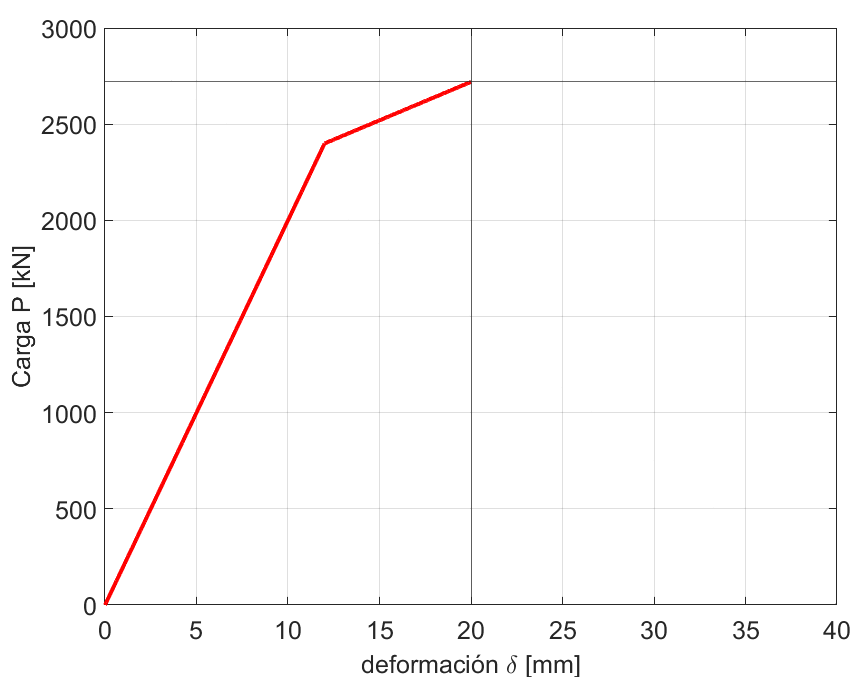
\includegraphics[width=0.55\linewidth]{Figuras/curvCapacidad.png}
\end{figure}

\noindent En la figura, haciendo click en file > export setup, se puede configurar la vista de la figura para exportar.

\subsection{Dispersión}
\begin{verbatimg}
    figure
    scatter(data_x, data_y)
\end{verbatimg}

\subsection{Histogramas}
\begin{verbatimg}
    figure
    histogram(vector_data)
\end{verbatimg}

\noindent También se pueden normalizar los histogramas y hacer ajustes a distribuciones

\begin{verbatimg}
    mu = 79.91;
    sigma = 14.89;
    cantidad_realizaciones = 1000;
    realizaciones_masas = normrnd(mu, sigma, cantidad_realizaciones, 1);

    % Histograma normalizado a pdf
    figure
    histogram(realizaciones_masas, 'normalization', 'pdf')

    % Histograma con ajuste de distribución
    figure
    histfit(realizaciones_masas, 20, 'normal')
    
\end{verbatimg}

\newpage
\noindent El resultado de aplicar \emph{histfit()} con las 1000 realizaciones (simulaciones) de la distribución normal.
\begin{figure}[H]
    \centering
    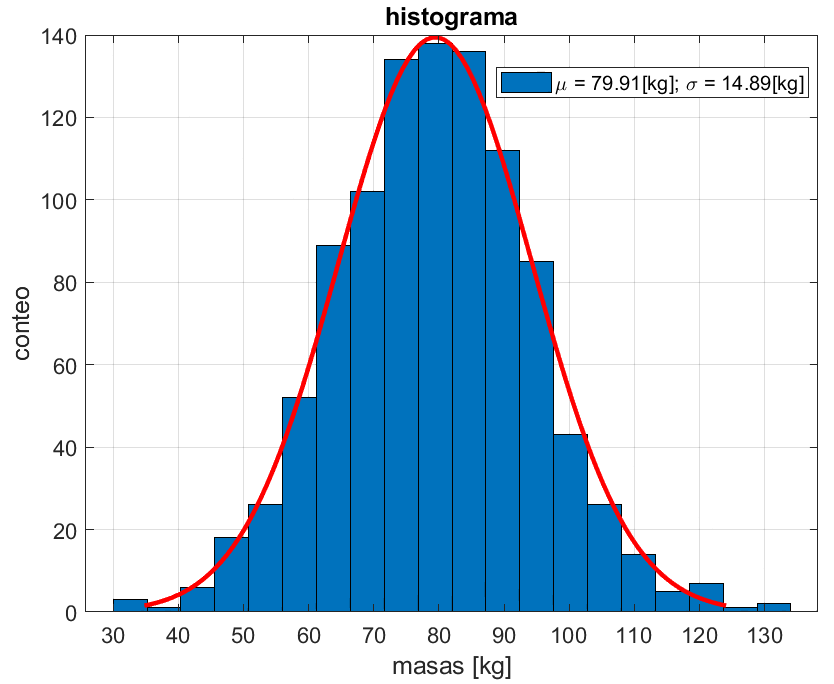
\includegraphics[width=0.55\linewidth]{Figuras/histogramFitting.png}
\end{figure}

\section{Instalar Toolbox}
Para instalar un toolbox, dentro de MATLAB ir a Home > Add-Ons > Get Add-Ons, lo que abrirá una pestaña para buscar e instalar toolbox.

\begin{figure}[H]
  \centering
  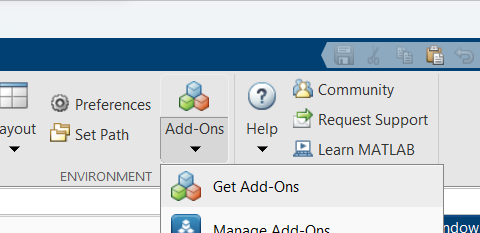
\includegraphics[width=0.47\textwidth]{Figuras/AddOnsButton.png} 
\end{figure}

Un toolbox necesario para el curso es el \emph{Control System}. Instalarlo.
\begin{figure}[H]
    \centering
    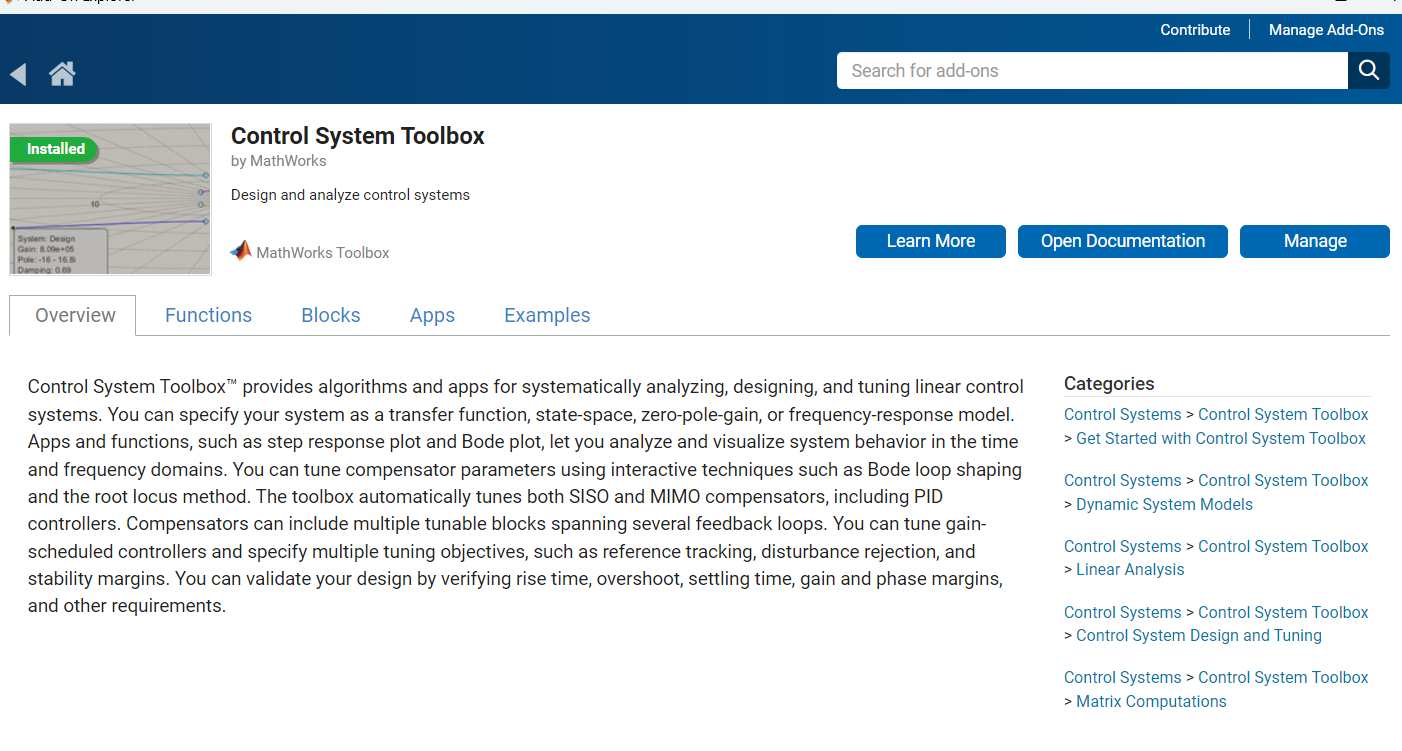
\includegraphics[width=0.75\linewidth]{Figuras/controlSystemToolbox.png}
\end{figure}

\section{Funciones útiles para el curso}
Muchos de los conceptos que se aprenden en cátedra, pueden realizarse en MATLAB con una función. \\

\subsection{Representación de sistemas}
Para trabajar con sistemas en MATLAB, existen las \emph{Variables tipo sistema} que pueden ser creadas con alguna de las repreentaciones vistas en clases (y más). \\

Espacio-Estado (State-Space, SS)
\begin{verbatimg}
    % Ass, Bss, Css, Dss son las matrices de la representación espacio-estado de un sistema
    sys_ss = ss(Ass, Bss, Css, Dss)
\end{verbatimg}

Función de Transferencia (Transfer Function, TF)
\begin{verbatimg}
    % num: vector con los coeficientes del polinomio del numerador de la TF
    % den: vector con los coeficientes del polinomio del denominador de la TF
    sys_tf = tf(num, den);
\end{verbatimg}

Desde State-Space a Transfer Function y viceversa
\begin{verbatimg}
    sys = ss(sys_tf);       % desde sistema en representación TF a SS
    sys = tf(sys_ss);       % desde sistema en representación SS a TF
    sys = ss2tf(A,B,C,D)    % tf desde matrices ss
    sys = tf2ss(num, den)   % ss desde coeficientes tf
\end{verbatimg}

\noindent Da exactamente el mismo sistema si se utiliza la representación state-space o transfer function.

\subsection{Excitar sistemas}
\begin{itemize}
    \item \emph{impulse(sys)}: aplicar impulso al sistema
    \item \emph{ramp(sys)}: aplicar excitación de rampa al sistema
    \item \emph{step(sys)}: aplicar excitación de escalón al sistema
\end{itemize}

\subsection{Otras funciones útiles para el curso}
\begin{itemize}
    \item \emph{damp()} - Polos, frecuencia, amortiguamiento
    \item \emph{bode(), bodeplot()} - Bode
    \item \emph{rootlocus()} - Root-locus
    \item \emph{pzmap()} - Mapa de polos y ceros
    \item \emph{fft(), shiftfft()} - Fast Fourier Transform
    \item \emph{ode45()} - Integración numérica Runge-Kutta Ode4
    \item \emph{expm()}
    \item \emph{repmat()}
\end{itemize}

\noindent Revisar la documentación de estas funciones


\chapter{Introducción a Simulink}

\section{Generalidades}

Simulink es una herramienta de \emph{MATLAB} que permite modelar, simular y analizar sistemas dinámicos mediante un enfoque de programación gráfica. 

El usuario construye el modelo conectando bloques que representan operaciones matemáticas, sistemas físicos o funciones lógicas. 
Las conexiones entre bloques representan señales, que transmiten información en forma de variables que evolucionan en el tiempo.

En Simulink, una \textbf{señal} puede ser escalar, vectorial o matricial. Su \emph{dimensión} y tipo de dato dependen del bloque que la genera y de la configuración del modelo. En términos generales, puede pensarse como un arreglo que cambia con el tiempo.

La Figura \ref{fig:simulink-ej} muestra un ejemplo sencillo de un modelo en Simulink.

\begin{figure}[h!]
    \centering
    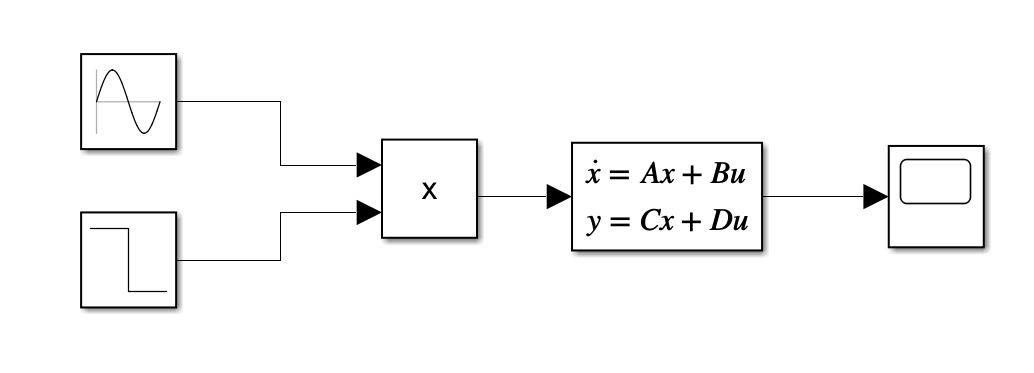
\includegraphics[width=0.7\textwidth]{placeholder_generalidades.png}
    \caption{Ejemplo de modelo simple en Simulink.}
    \label{fig:simulink-ej}
\end{figure}

\section{Entradas}
Las entradas permiten excitar el sistema o modelo. Simulink ofrece diversos bloques para generar señales de entrada.

\subsection{Constante}
El bloque \textbf{Constant} genera una señal con valor constante durante toda la simulación, como se muestra en la Figura \ref{fig:simulink-cte}.

\begin{figure}[h!]
    \centering
    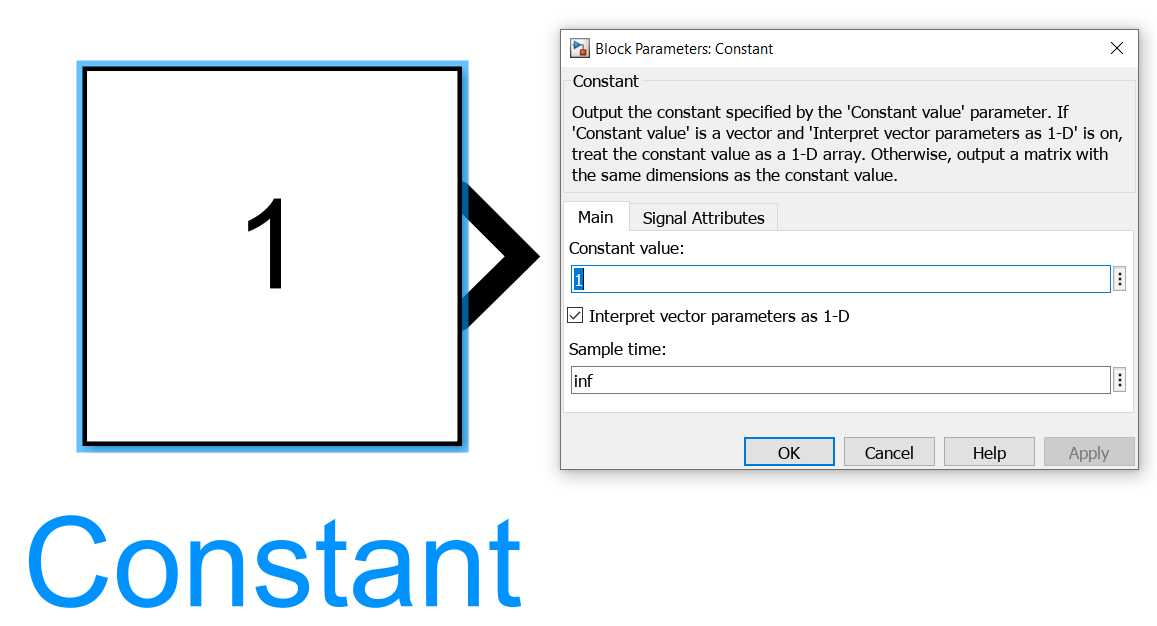
\includegraphics[width=0.5\textwidth]{bloque constant.png}
    \caption{Bloque de entrada constante.}
    \label{fig:simulink-cte}
\end{figure}

\subsection{Seno}
El bloque \textbf{Sine Wave} genera una señal sinusoidal con amplitud, frecuencia y fase configurables, como se muestra en las Figuras \ref{fig:simulink-sine} y \ref{fig:simulink-prop-sine}.

\begin{figure}[h!]
    \centering
    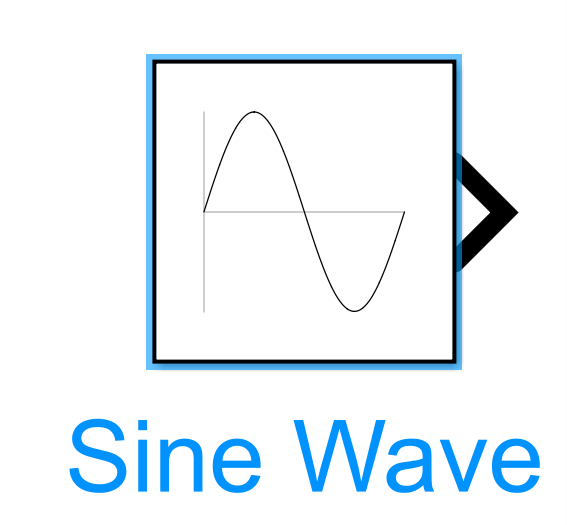
\includegraphics[width=0.2\textwidth]{Figuras/bloque seno.png}
    \caption{Bloque de entrada Seno.}
    \label{fig:simulink-sine}
\end{figure}

\begin{figure}[h!]
    \centering
    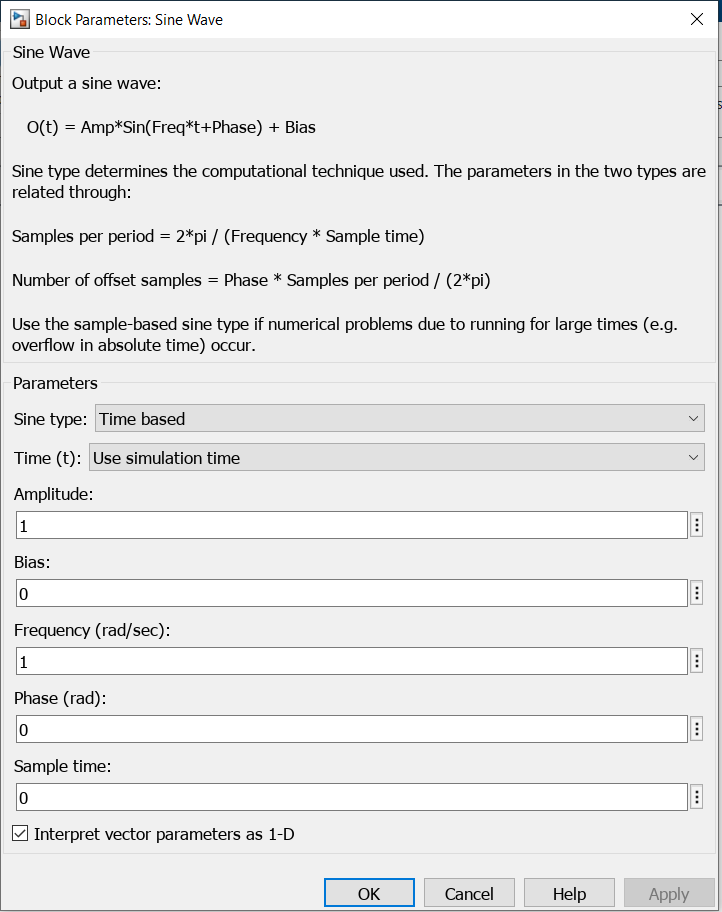
\includegraphics[width=0.5\textwidth]{Figuras/parametros seno.png}
    \caption{Parámetros de entrada Seno.}
    \label{fig:simulink-prop-sine}
\end{figure}

\subsection{Rampa}
El bloque \emph{Ramp} produce una señal de tipo rampa lineal, útil para representar entradas que crecen con pendiente constante, donde, como se muestra en la Figura \ref{fig:simulink-para-ramp} se puede configurar tanto la pendiente como el intervalo donde inicia la señal. El bloque se muestra en la Figura \ref{fig:simulink-ramp}.

\begin{figure}[h!]
    \centering
    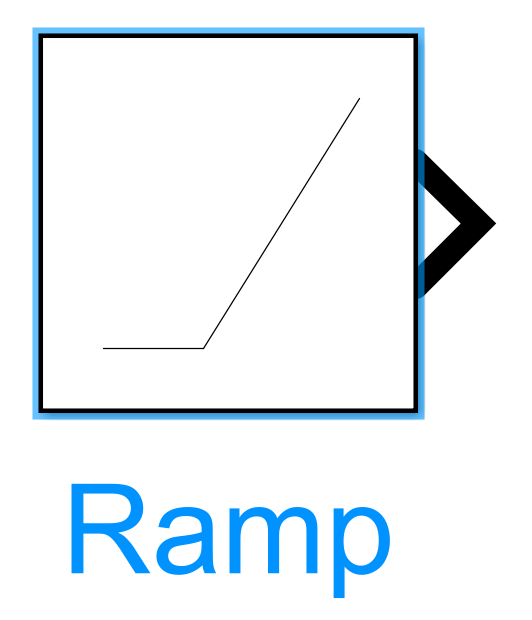
\includegraphics[width=0.2\textwidth]{Figuras/bloque ramp.png}
    \caption{Bloque Ramp.}
    \label{fig:simulink-ramp}
\end{figure}

\begin{figure}[h!]
    \centering
    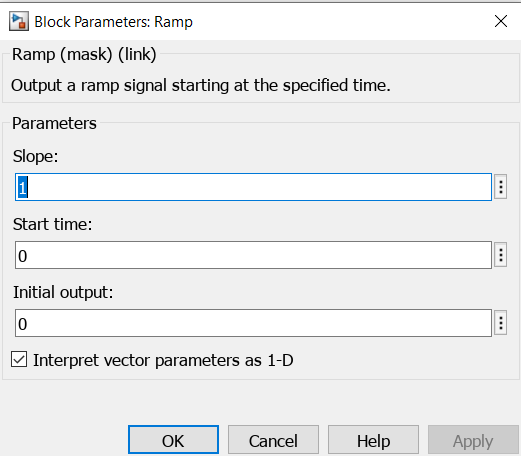
\includegraphics[width=0.5\textwidth]{Figuras/parametros ramp.png}
    \caption{Parámetros Ramp.}
    \label{fig:simulink-para-ramp}
\end{figure}

\subsection{Ruido blanco}
El bloque \textbf{Band-Limited White Noise} permite generar ruido blanco, empleado en análisis de respuesta a señales aleatorias. Como se muestra en la Figura \ref{fig:simulink-blwn}.

\begin{figure}[h!]
    \centering
    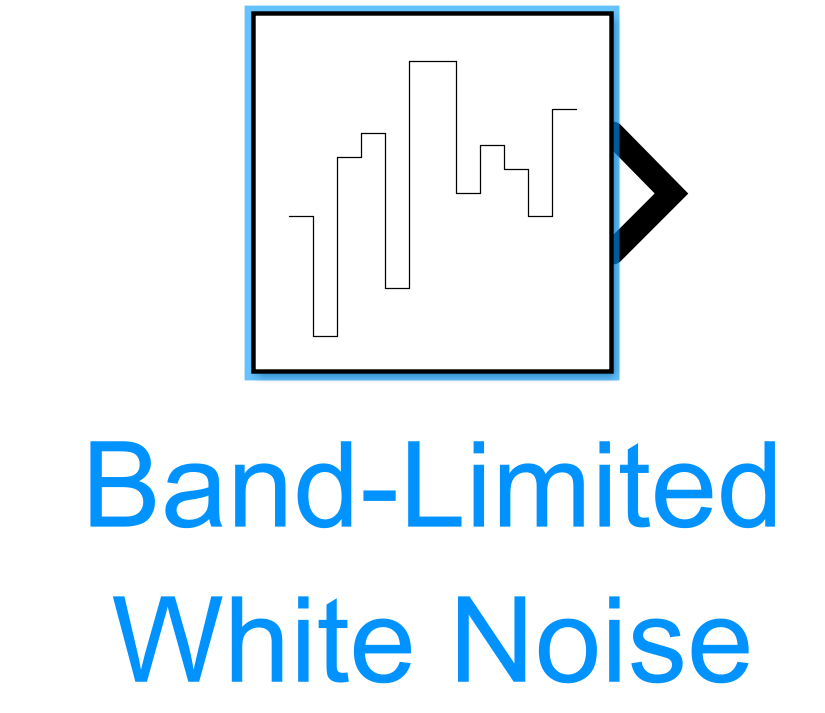
\includegraphics[width=0.25\textwidth]{Figuras/bloque ruido blanco.png}
    \caption{Bloque de entrada Ruido Blanco de Banda Limitada.}
    \label{fig:simulink-blwn}
\end{figure}

Para emplear este bloque es necesario contar con la densidad espectral de potencia, la frecuencia de muestro asociada y un valor de semilla que permita generar el ruido no correlacionado. Como se Muestra en la Figura \ref{fig:simulink-parameterblwn}.

\begin{figure}[h!]
    \centering
    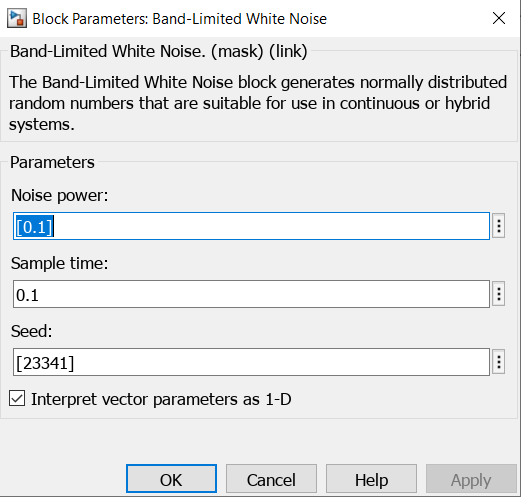
\includegraphics[width=0.5\textwidth]{Figuras/parametros ruido blanco.png}
    \caption{parámetros de entrada Ruido Blanco de Banda Limitada.}
    \label{fig:simulink-parameterblwn}
\end{figure}

\subsection{\emph{From workspace}}
Este bloque permite incorporar variables previamente definidas en el espacio de trabajo (\emph{workspace}) de MATLAB y asignar como señales en \emph{Simulink}, facilitando la simulación con datos experimentales o precomputados.
La variable cargada desde el espacio de trabajo debe estructurarse como una matriz de dos columnas: la primera indica los instantes de tiempo y la segunda los valores de la señal. Si la duración de la simulación excede el rango temporal de los datos, los valores deben prolongarse como cero, evitando en todo momento el uso de la opción de “extrapolación”. El bloque y sus parámetros se muestran en las Figuras \ref{fig:simulink-workspace} y \ref{fig:simulink-para-workspace}

\begin{figure}[h!]
    \centering
    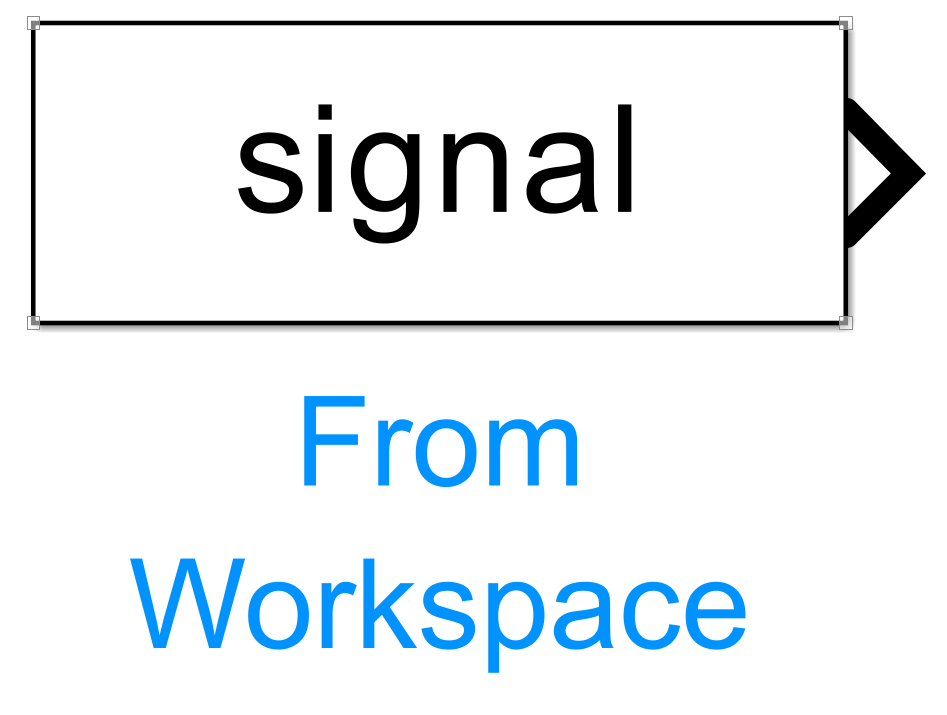
\includegraphics[width=0.25\textwidth]{Figuras/bloque from workspace.png}
    \caption{Bloque de entrada del Espacio de Trabajo.}
    \label{fig:simulink-workspace}
\end{figure}

\begin{figure}[h!]
    \centering
    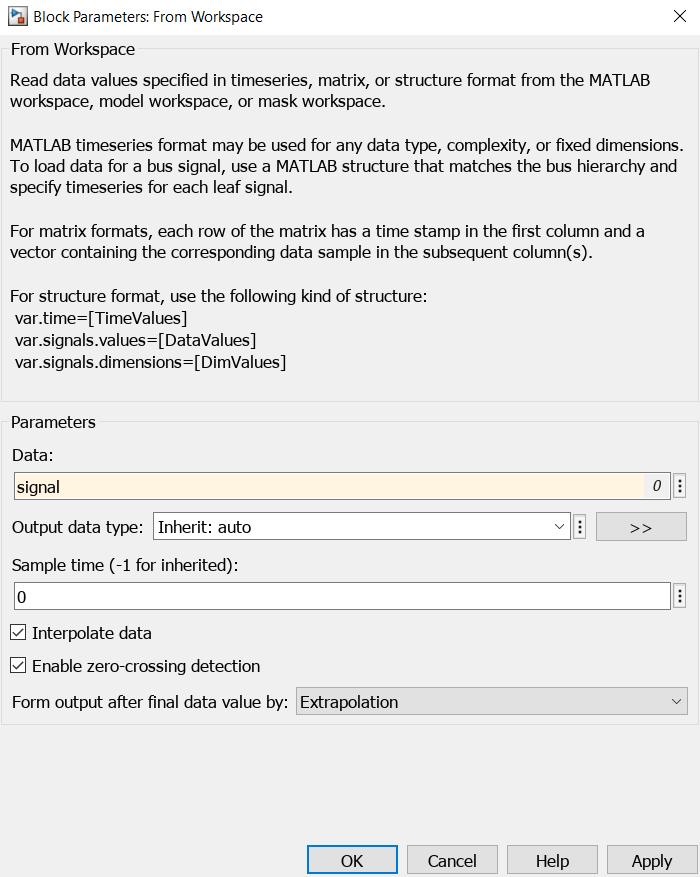
\includegraphics[width=0.5\textwidth]{Figuras/parametros from workspace.png}
    \caption{Parámetros de entrada del Espacio de Trabajo.}
    \label{fig:simulink-para-workspace}
\end{figure}

\section{Operaciones}
Los bloques de operaciones permiten transformar señales mediante operaciones matemáticas básicas.

\subsection{Suma}
El bloque \textbf{Sum} combina varias señales mediante suma o resta, dependiendo de la configuración de sus entradas. Como se muestra en la Figura \ref{fig:simulink-suma}.

\begin{figure}[h!]
    \centering
    
\includegraphics[width=0.25\textwidth]{Figuras/bloque sum.png}
    \caption{Bloque de Suma.}
    \label{fig:simulink-suma}
\end{figure}

El número de entradas, su posición dentro del bloque y su signo pueden modificarse agregando los símbolos ‘+’, ‘–’ y '\textbar '

\subsection{Multiplicación}
El bloque \textbf{Product} multiplica dos señales entre sí. Es posible configurarlo para modificar el número de entradas y definir si la operación entre ellas corresponde a una multiplicación escalar o matricial. Como se muestra en la Figura \ref{fig:simulink-product}

\begin{figure}[h!]
    \centering
    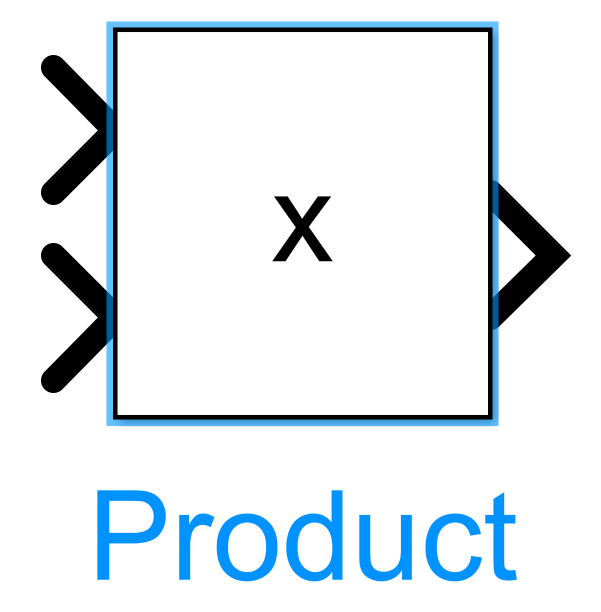
\includegraphics[width=0.2\textwidth]{Figuras/bloque product.png}
    \caption{Bloque Producto.}
    \label{fig:simulink-product}
\end{figure}

\subsection{Gain}
El bloque \textbf{Gain} aplica una ganancia constante a una señal de entrada, mostrado en la Figura \ref{fig:simulink-gain}. Este bloque, al igual que \textbf{Product}, admite multiplicación escalar o matricial, con la opción adicional de cambiar el orden en la operación matricial. Como se muestra en la Figura \ref{fig:simulink-parametros-gain}.

\begin{figure}[h!]
    \centering
    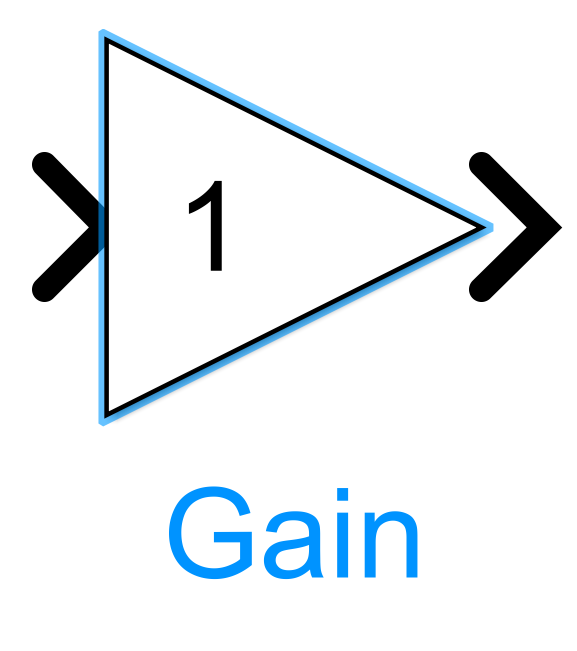
\includegraphics[width=0.2\textwidth]{Figuras/bloque gain.png}
    \caption{Bloque Ganancia.}
    \label{fig:simulink-gain}
\end{figure}

\begin{figure}[h!]
    \centering
    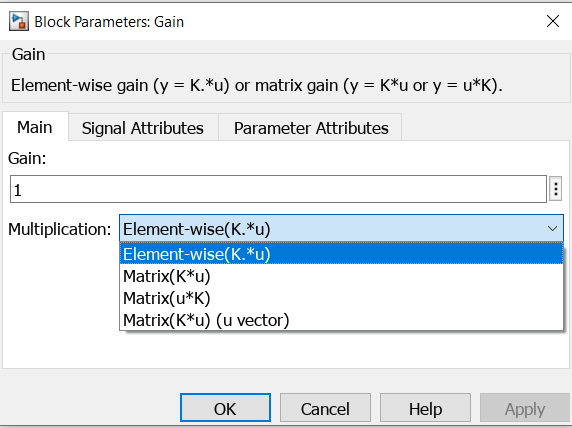
\includegraphics[width=0.6\textwidth]{Figuras/parametros gain.png}
    \caption{Parámetros Ganancia.}
    \label{fig:simulink-parametros-gain}
\end{figure}

\subsection{Integración}
El bloque \textbf{Integrator}, mostrado en la Figura \ref{fig:simulink-int}. calcula la integral de la señal de entrada, representando sistemas dinámicos como masas, resortes o cargas acumuladas. Este bloque permite definir la condición inicial de la integración, ofrece la posibilidad de establecer límites superior e inferior mediante saturación, y cuenta con configuraciones adicionales para el manejo de la salida y la opción de reiniciar el integrador. Como se muestra en la Figura \ref{fig:simulink-para-int}.

\begin{figure}[h!]
    \centering
    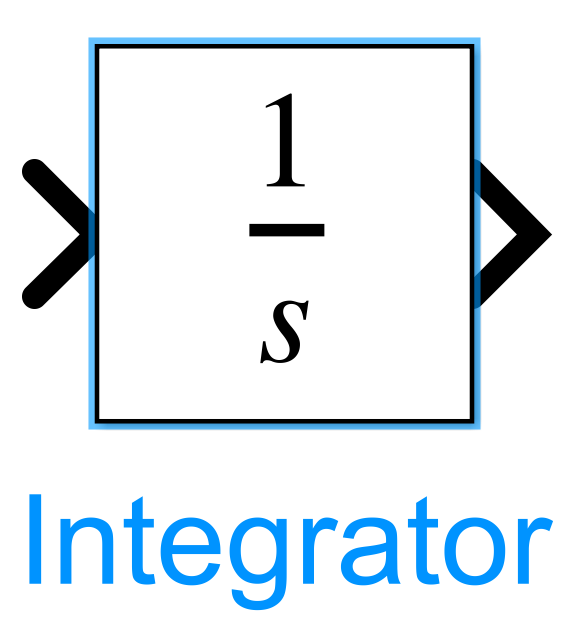
\includegraphics[width=0.2\textwidth]{Figuras/bloque integrator.png}
    \caption{Bloque Integración.}
    \label{fig:simulink-int}
\end{figure}

\begin{figure}[h!]
    \centering
    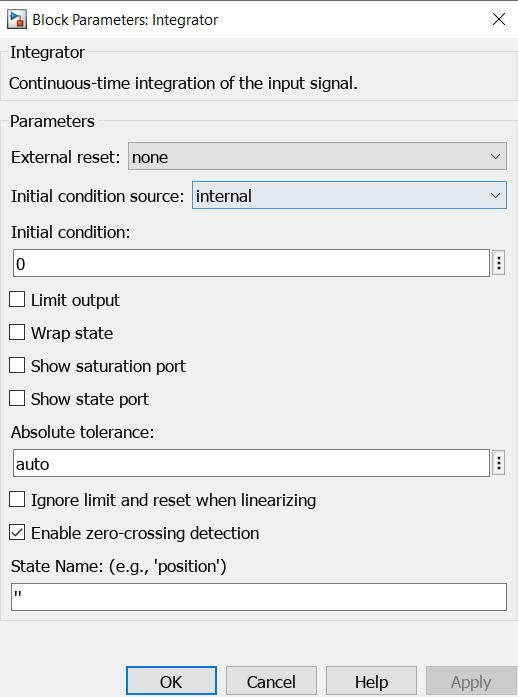
\includegraphics[width=0.5\textwidth]{Figuras/parametros integrator.png}
    \caption{Parámetros bloque integración.}
    \label{fig:simulink-para-int}
\end{figure}

\section{Sistemas}
Simulink ofrece bloques para representar modelos dinámicos en distintas formas matemáticas.

\subsection{State-space}
El bloque \textbf{State-Space} permite implementar un sistema LTI en representación de variables de estado, definido por las matrices $A$, $B$, $C$ y $D$. Como se muestra en las Figuras \ref{fig:simulink-ss}. y \ref{fig:simulink-para-ss}.

\begin{figure}[h!]
    \centering
    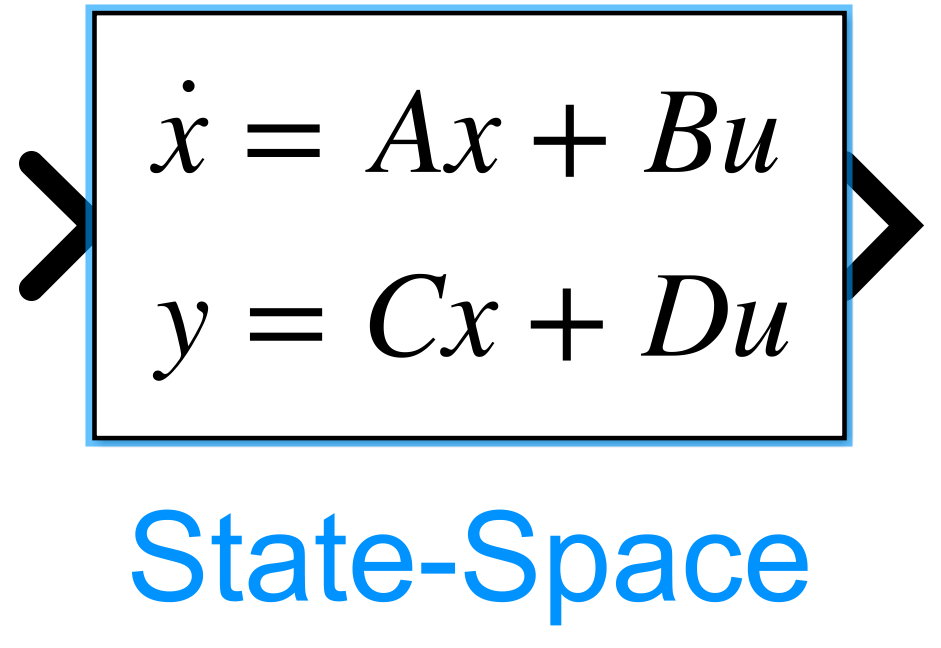
\includegraphics[width=0.2\textwidth]{Figuras/bloque espacio estado.png}
    \caption{Bloque Espacio-estado.}
    \label{fig:simulink-ss}
\end{figure}

\begin{figure}[h!]
    \centering
    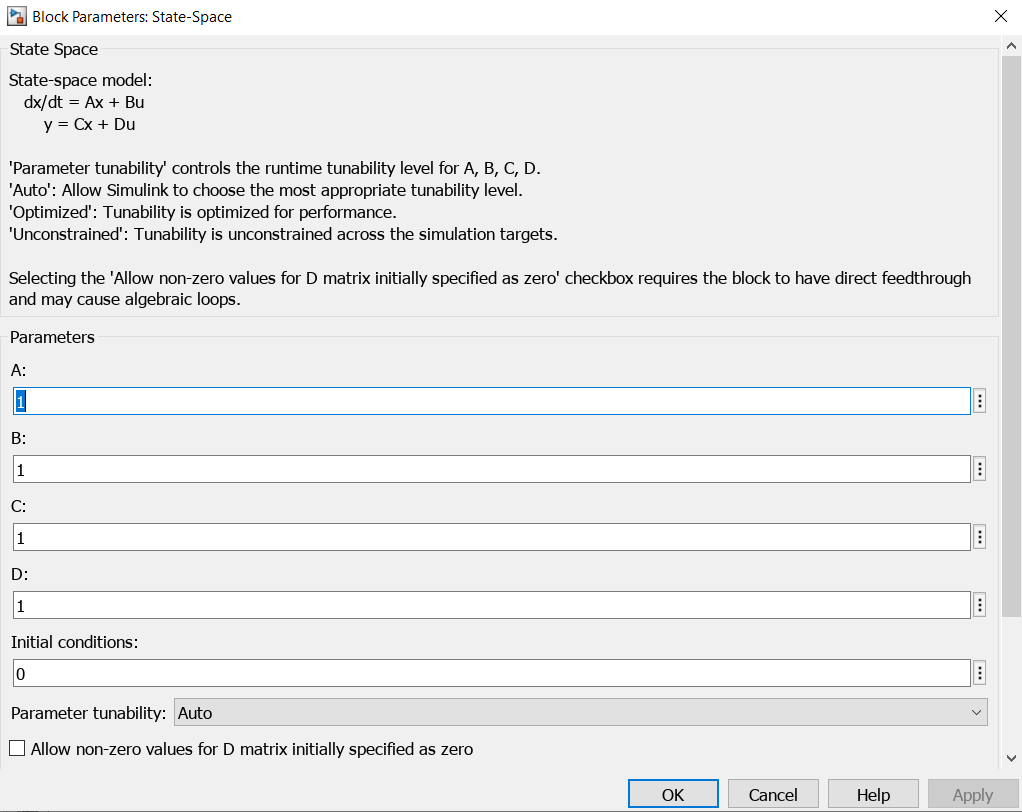
\includegraphics[width=0.6\textwidth]{Figuras/parametros espacio estado.png}
    \caption{Parámetros Espacio-estado.}
    \label{fig:simulink-para-ss}
\end{figure}

% \textit{Nota: Si una matriz contiene únicamente ceros, debe ingresarse respetando su dimensión completa y no como un valor escalar igual a cero.}

\subsection{Transfer function}
El bloque \textbf{Transfer Function} implementa sistemas definidos mediante funciones de transferencia, expresadas como el cociente de polinomios en $s$, como se muestra en la Figura \ref{fig:simulink-tf}. Los parámetros a ingresar en el bloque se muestran en la Figura \ref{fig:simulink-parametrostf}.

\begin{figure}[h!]
    \centering
    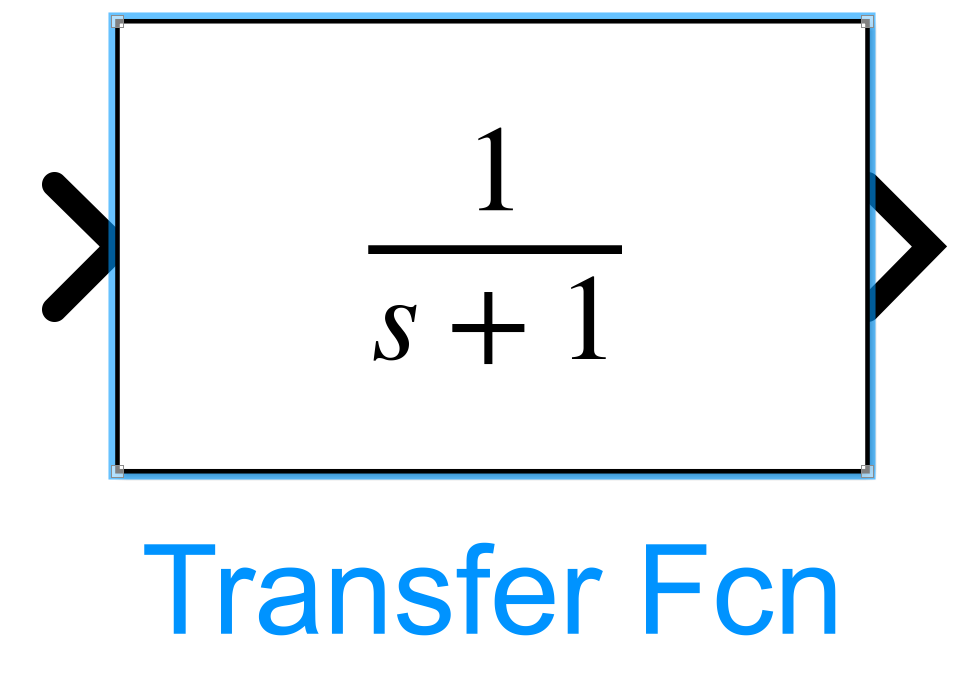
\includegraphics[width=0.2\textwidth]{Figuras/bloque transfer funtion.png}
    \caption{Bloque Función de transferencia.}
    \label{fig:simulink-tf}
\end{figure}

\begin{figure}[h!]
    \centering
    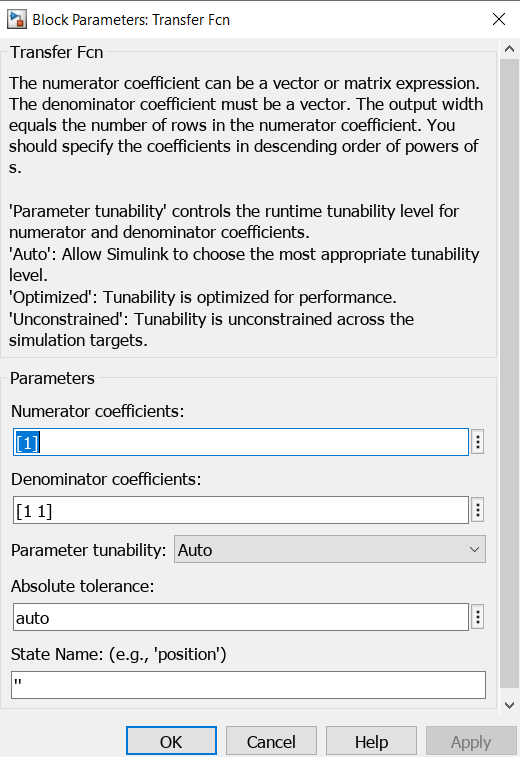
\includegraphics[width=0.5\textwidth]{Figuras/parametros trans fun.png}
    \caption{Parámetros Trasnsfer Function.}
    \label{fig:simulink-parametrostf}
\end{figure}

\subsection{Matlab Function}
En algunos casos, es necesario generar señales complejas o no lineales que no pueden obtenerse sólo con bloques estándar. 
El bloque \textbf{MATLAB Function} permite definir una función que recibe una señal de entrada y produce una salida calculada en código MATLAB. El bloque se muestra en la Figura \ref{fig:simulink-matfun}.

Este bloque permite integrar funciones escritas en MATLAB directamente en un modelo, ejecutando código personalizado durante la simulación. Su sintaxis se muestra en la Figura \ref{fig:simulink-para-matfun}.

\begin{figure}[h!]
    \centering
    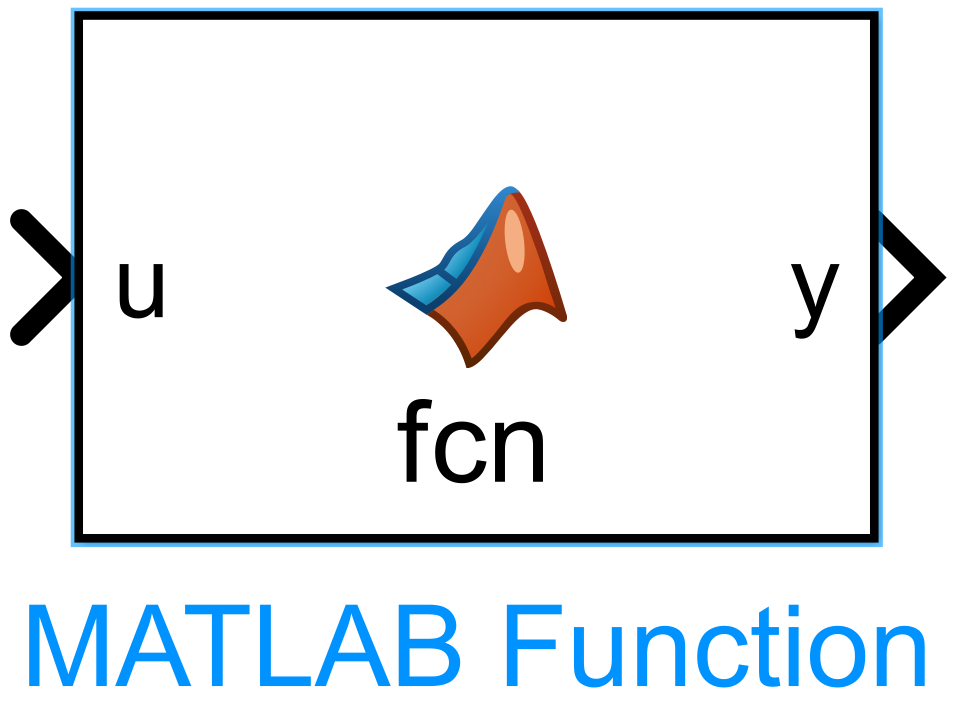
\includegraphics[width=0.2\textwidth]{Figuras/bloque mat fun.png}
    \caption{Bloque Función de Matlab.}
    \label{fig:simulink-matfun}
\end{figure}

\begin{figure}[h!]
    \centering
    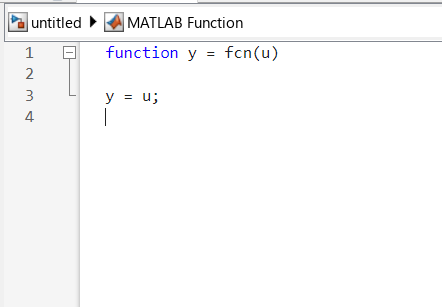
\includegraphics[width=0.5\textwidth]{Figuras/parametros mat fun.png}
    \caption{Parámetros Bloque Función de Matlab.}
    \label{fig:simulink-para-matfun}
\end{figure}

\section{Salidas}
Las salidas permiten visualizar, registrar o exportar los resultados de la simulación.

\subsection{Scope}
El bloque \textbf{Scope} es un osciloscopio virtual que muestra la evolución temporal de las señales durante la simulación. La Figura \ref{fig:simulink-ver-scope} muestra una señal sinusoidal de entrada..

\begin{figure}[h!]
    \centering
    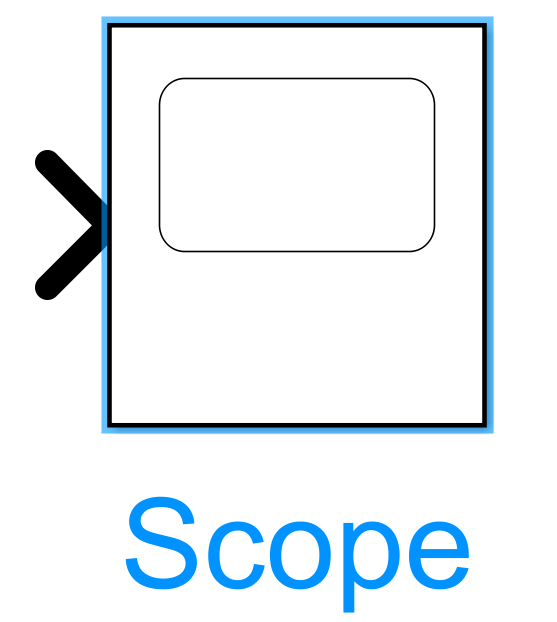
\includegraphics[width=0.2\textwidth]{Figuras/bloque scope.png}
    \caption{Bloque Scope.}
    \label{fig:simulink-scope}
\end{figure}

\begin{figure}[h!]
    \centering
    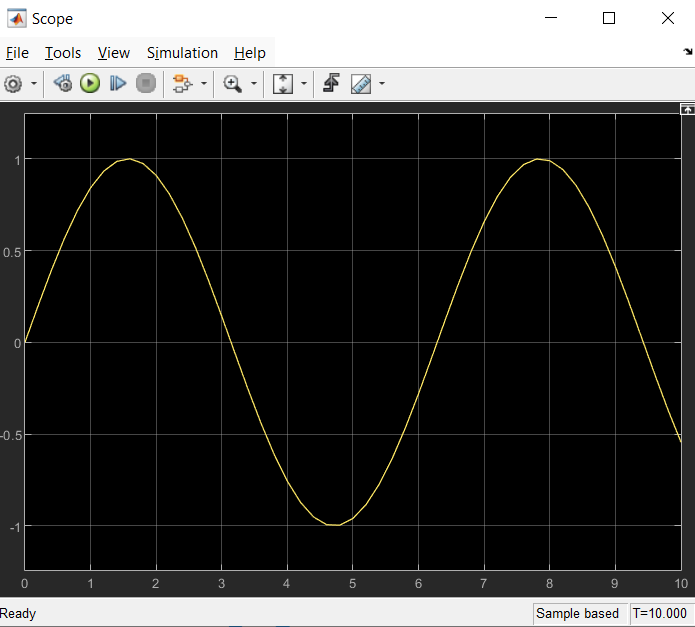
\includegraphics[width=0.5\textwidth]{Figuras/parametros scope.png}
    \caption{Visualización Scope.}
    \label{fig:simulink-ver-scope}
\end{figure}

\subsection{\emph{To workspace}}
Este bloque permite exportar las señales al \emph{workspace} de MATLAB, para su posterior análisis o graficación. Como se muestra en la Figura \ref{fig:simulink-toworkspace}.

\begin{figure}[h!]
    \centering
    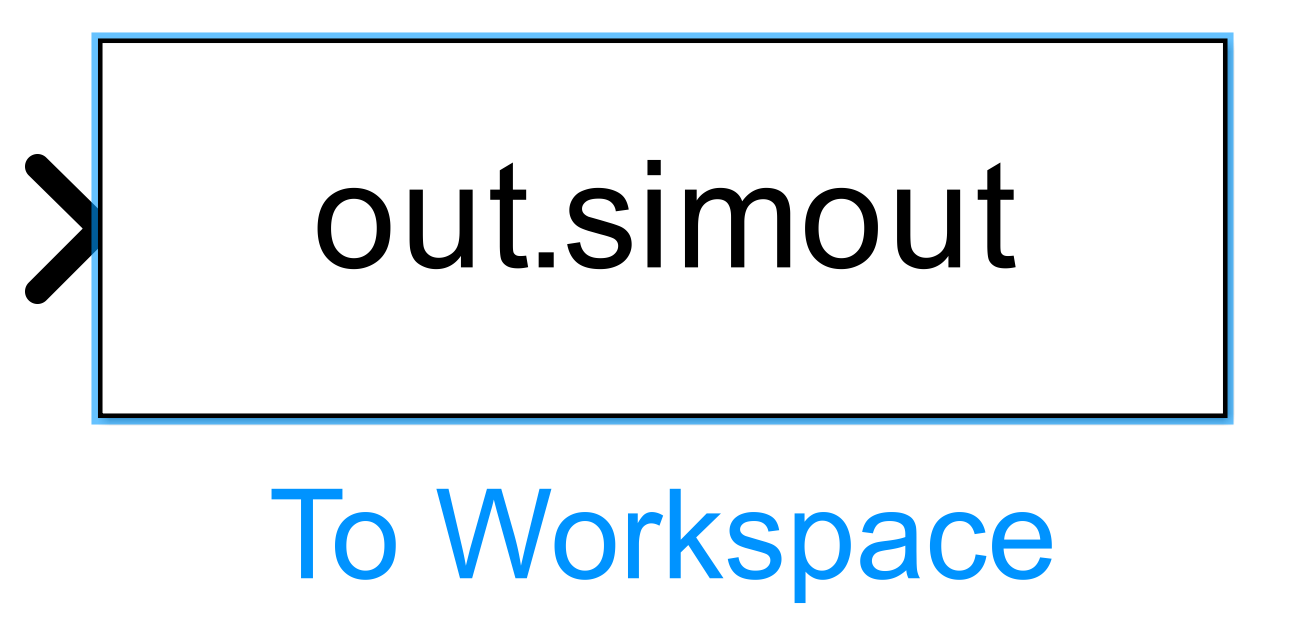
\includegraphics[width=0.2\textwidth]{Figuras/bloque to workspace.png}
    \caption{Bloque To workspace.}
    \label{fig:simulink-toworkspace}
\end{figure}

\section{Propiedades simulación}
Antes de ejecutar un modelo, es necesario configurar sus parámetros de simulación: 
tiempo inicial $t_\text{init}$, tiempo final $t_\text{end}$ y paso de integración $t_\text{step}$. 
Simulink ofrece distintos métodos de integración (\emph{fixed-step} y \emph{variable-step}) y algoritmos como Runge-Kutta de cuarto orden (\texttt{ode4}). Esta configuración se encuentra en la sección mostrada en la Figura \ref{fig:simulink-parametros-simulacion}.

\begin{figure}[H]
    \centering
    
    % Subimagen 1
    \begin{subfigure}
        \centering
        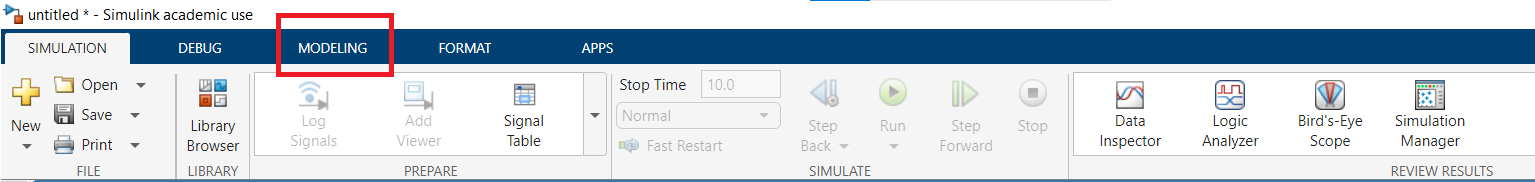
\includegraphics[width=\linewidth]{propiedades1.png}
    \end{subfigure}
    
    % Subimagen 2
    \begin{subfigure}
        \centering
        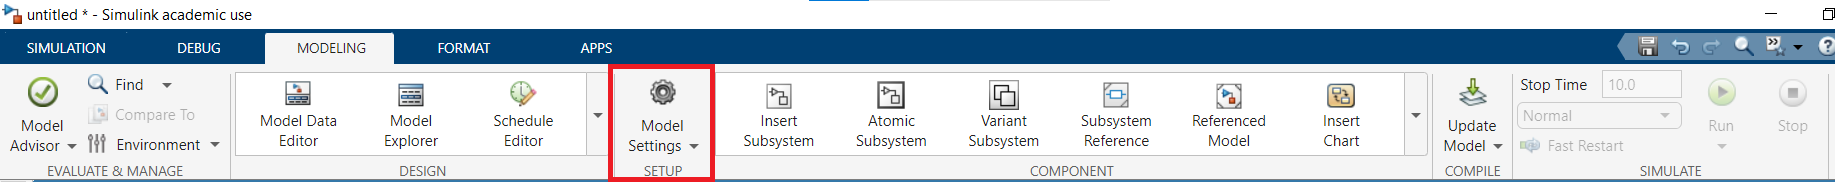
\includegraphics[width=\linewidth]{propiedades2.png}
    \end{subfigure}
    
    % Subimagen 3
    \begin{subfigure}
        \centering
        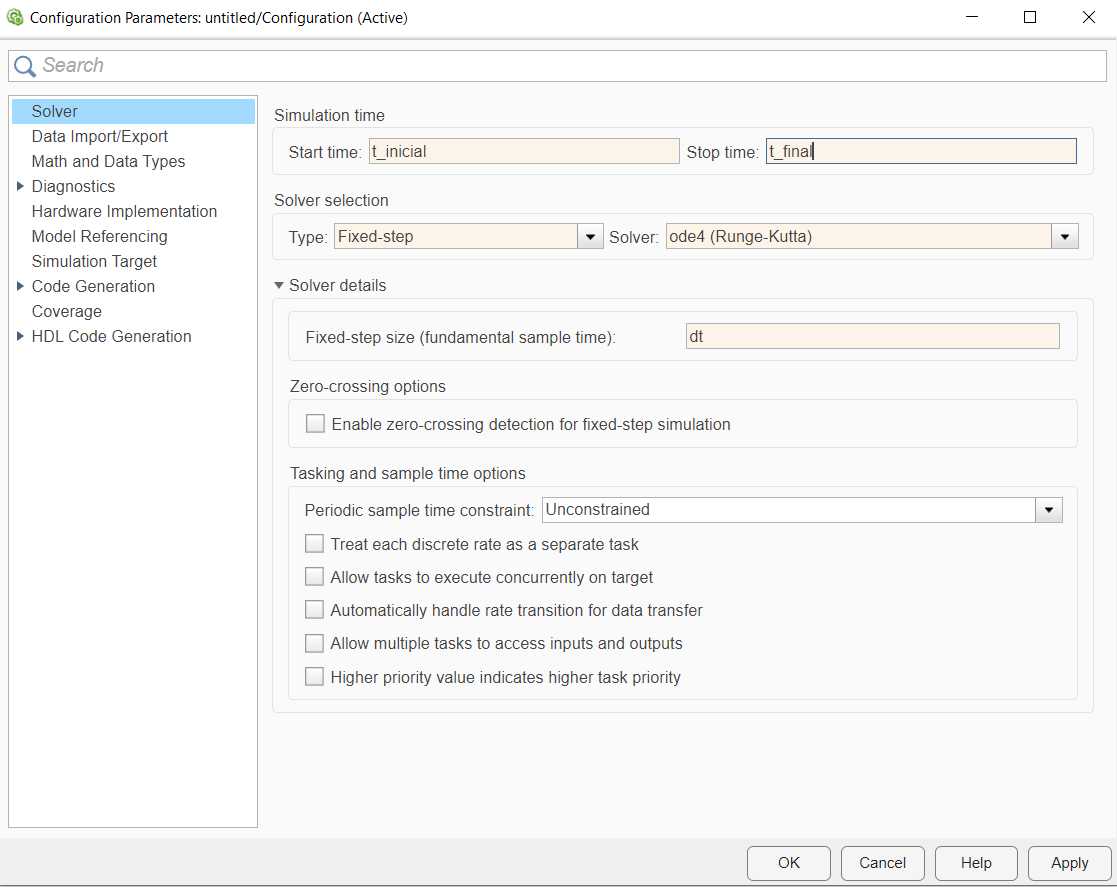
\includegraphics[width=\linewidth]{propiedades3.png}
    \end{subfigure}

    \caption{Configuración parámetros de Simulación}
    \label{fig:simulink-parametros-simulacion}
\end{figure}

\section{Bloques especiales}

\subsection{Mux/Demux}
Los bloques \textbf{Mux} y \textbf{Demux} permiten agrupar y desagrupar señales, respectivamente. 
Son útiles para manejar señales vectoriales en diagramas complejos. Ambos bloques se muestran en la Figura \ref{fig:simulink-mux-demux}.

\begin{figure}[H]
    \centering
    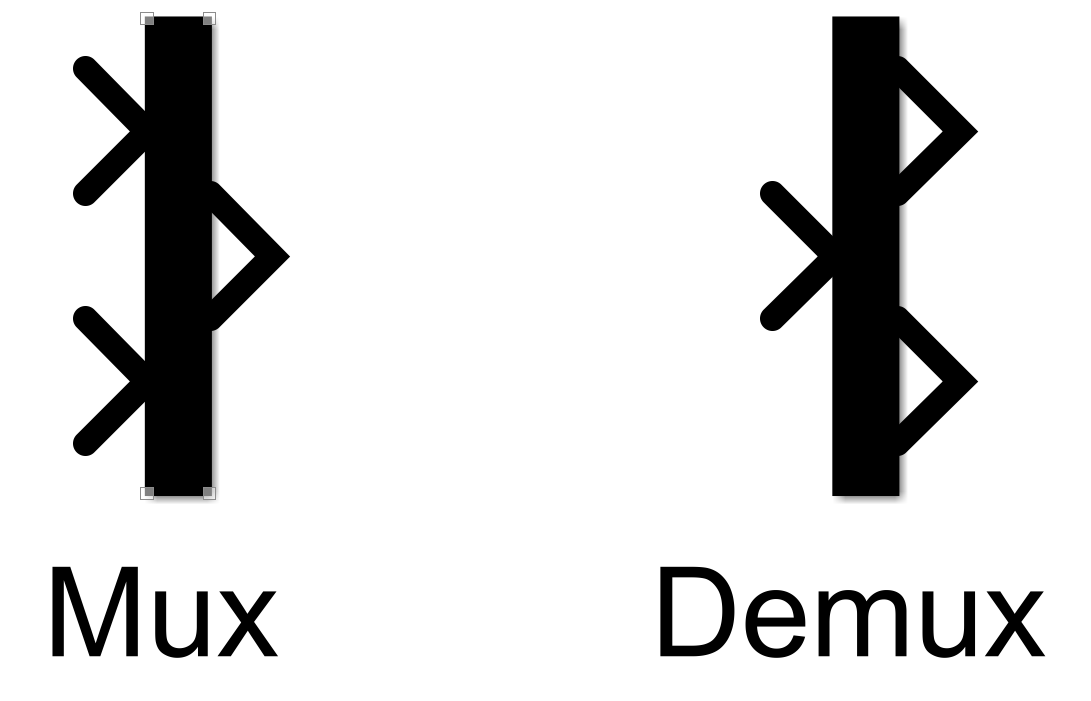
\includegraphics[width=0.2\textwidth]{Figuras/bloque mux demux.png}
    \caption{Bloque Mux y Demux.}
    \label{fig:simulink-mux-demux}
\end{figure}

\subsection{Selector}
El bloque \textbf{Selector} permite extraer componentes específicas de una señal vectorial o matricial, como se muestra en la Figura \ref{fig:simulink-selector}.

\begin{figure}[H]
    \centering
    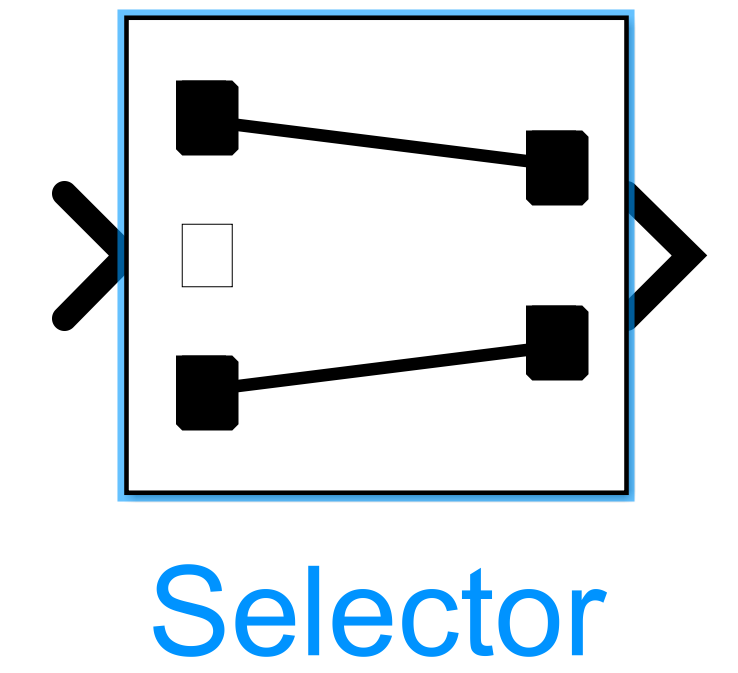
\includegraphics[width=0.2\textwidth]{Figuras/bloque selector.png}
    \caption{Bloque Selector.}
    \label{fig:simulink-selector}
\end{figure}

\subsection{\emph{Zero-order hold} (ZOH)}
El bloque \textbf{Zero-Order Hold} convierte señales continuas en discretas manteniendo el último valor de muestreo, lo que es esencial en sistemas mixtos continuo. El paso temporal se define en los parámetros como se muestra en la Figura \ref{fig:simulink-para-zoh}. Este bloque se muestra en la Figura \ref{fig:simulink-zoh}.

\begin{figure}[H]
    \centering
    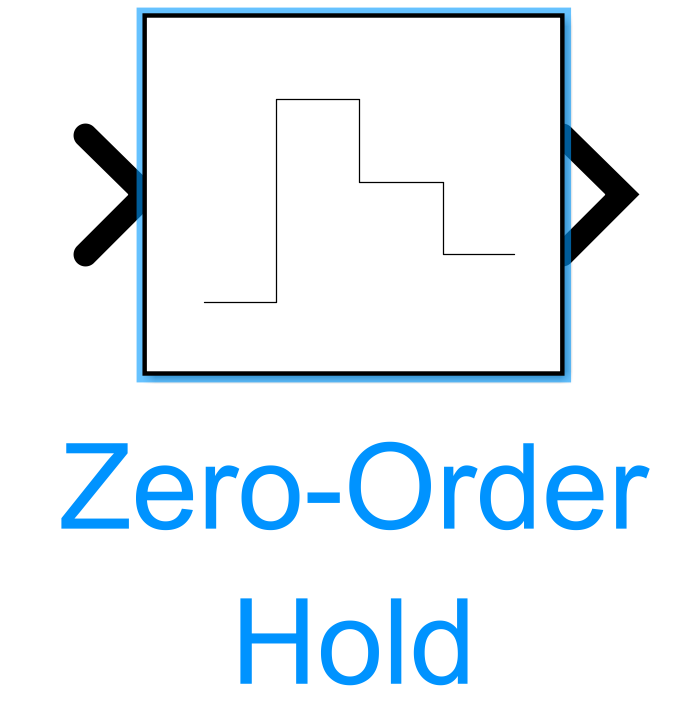
\includegraphics[width=0.2\textwidth]{Figuras/bloque zoh.png}
    \caption{Bloque Zoh.}
    \label{fig:simulink-zoh}
\end{figure}

\begin{figure}[H]
    \centering
    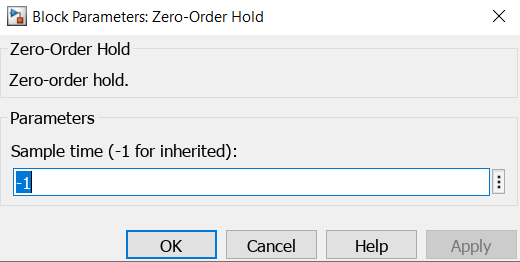
\includegraphics[width=0.5\textwidth]{Figuras/parametros zoh.png}
    \caption{Parámetros Zoh.}
    \label{fig:simulink-para-zoh}
\end{figure}

\section{Ejemplo}

Se realiza el ejemplo de un modelo de un grado de libertad sometido a una aceleración basal.
Inicialmente se definen los parámetros del sistema dinámico, masa, frecuencia natural y razón de amortiguamiento.

\begin{verbatimg}
%% Definir parametros

fn = 2; % Hz
m = 1000; % kg
zeta = 0.05;
\end{verbatimg}

A partir de los parámetros definidos se obtienen los coeficientes de la ecuación diferencial de movimiento asociada.

\begin{verbatimg}
%% Obtener EDM
% m*ddu + c*du + k*u = -m*ddug

wn = 2*pi*fn; % rad/s
k = wn^2*m; % N/m
c = 2*zeta*m*wn; % N-s/m
\end{verbatimg}

Luego se escribe en función de las ecuaciones de espacio estado. En este caso particular se quiere como salida el desplazamiento relativo, la velocidad relativa y la aceleración absoluta.

\begin{verbatimg}
%% Representacion Espacio Estado
% dx = As*x + Bs*ddug
%  y = Cs*x + Ds*ddug

Ass = [0 1; -k/m -c/m];
Bss = [0; -m/m];
Css = [1 0; 0 1; -k/m -c/m];
Dss = [0; 0; 0];
\end{verbatimg}

Después se lee el registro de aceleración y se crea una matriz con tiempo-aceleración.

\begin{verbatimg}
%% Leer registro aceleracion

record = importdata('RegistroNorthridge1994_TarzanaCH1.txt');
record.dt = 0.02;
record.N = length(record.data);
time = linspace(0,(record.N-1)*record.dt,record.N)';

acel = record.data/100; % en m/s2
acel_simu = [time,acel];

\end{verbatimg}

Se ajustan los parámetros de simulación, considerando un paso temporal de 0.001 s y se ajusta el tiempo de simulación al tiempo del registro de aceleración.

\begin{verbatimg}
%% Simulacion

t_muestreo = time(end); % tiempo final del registro sismico
dt = 1/1000; % s

\end{verbatimg}

Ya con los parámetros definidos se ingresan en la configuración de Simulink, se utiliza Runge-Kutta (ode4), como se muestra en la Figura \ref{fig:simulink-para-ejem}.

\begin{figure}[H]
    \centering
    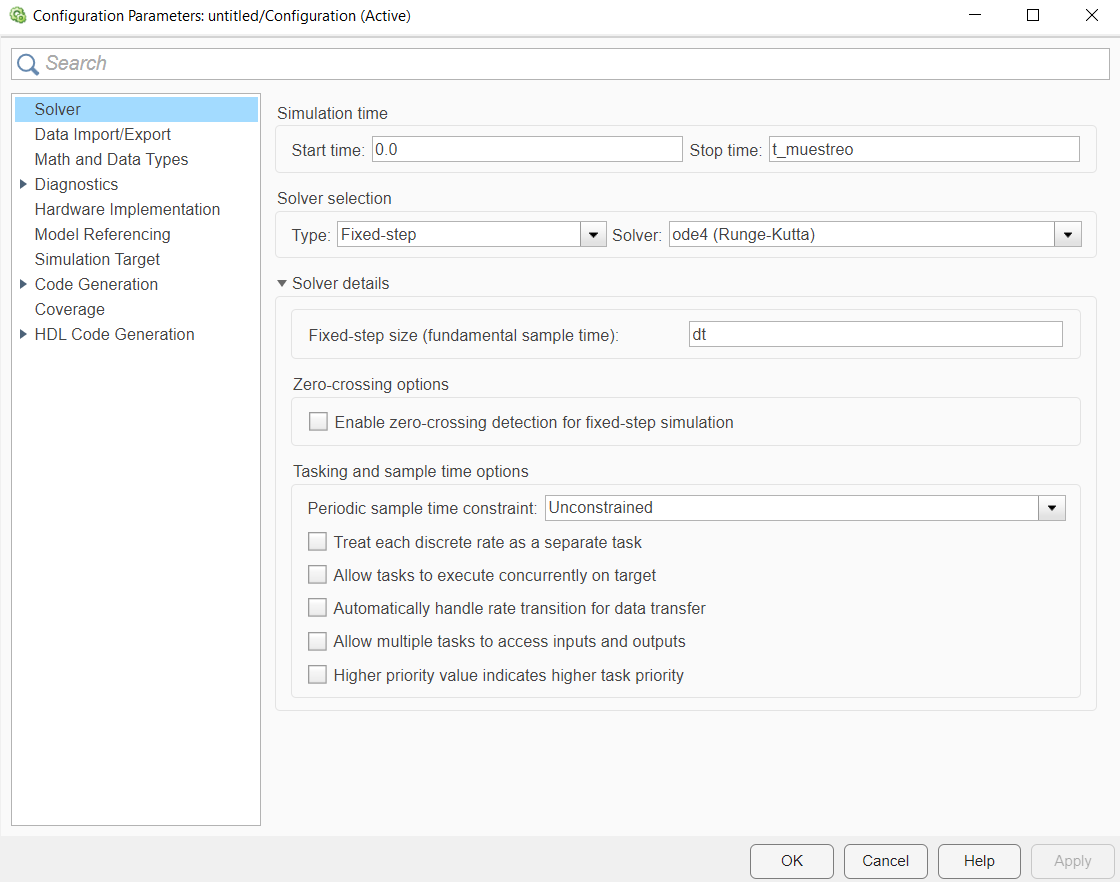
\includegraphics[width=0.8\textwidth]{Figuras/parametros simulacion ejemplo.png}
    \caption{Parámetros Simulación de Ejemplo.}
    \label{fig:simulink-para-ejem}
\end{figure}

Luego se modela la entrada como un bloque \textbf{from workspace}, como se muestra en la Figura \ref{fig:simulink-acel}. El sistema dinámico utilizando el bloque \textbf{state-space},como se muestra en la Figura \ref{fig:simulink-ss-ejemplo}, donde las salidas se separan utilizando un bloque \textbf{demux} para finalmente ser enviadas al espacio de trabajo utilizando el bloque \textbf{to workspace}. El sistema completo se muestra en la Figura \ref{fig:simulink-ejemplo}.

\begin{figure}[H]
    \centering
    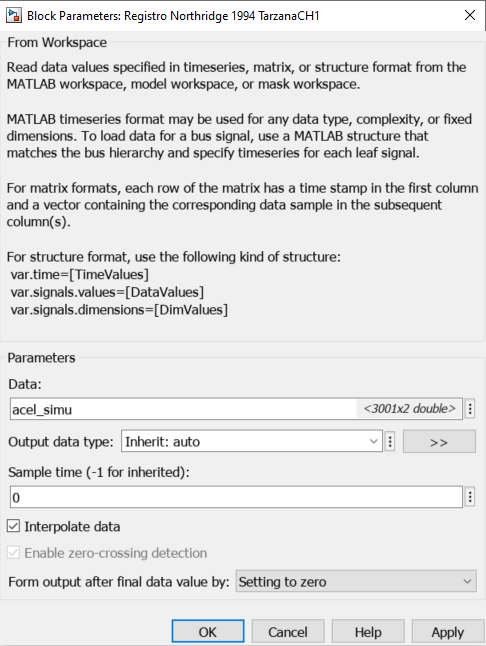
\includegraphics[width=0.5\textwidth]{Figuras/aceleracion ejemplo.png}
    \caption{Registro de Aceleración.}
    \label{fig:simulink-acel}
\end{figure}

\begin{figure}[H]
    \centering
    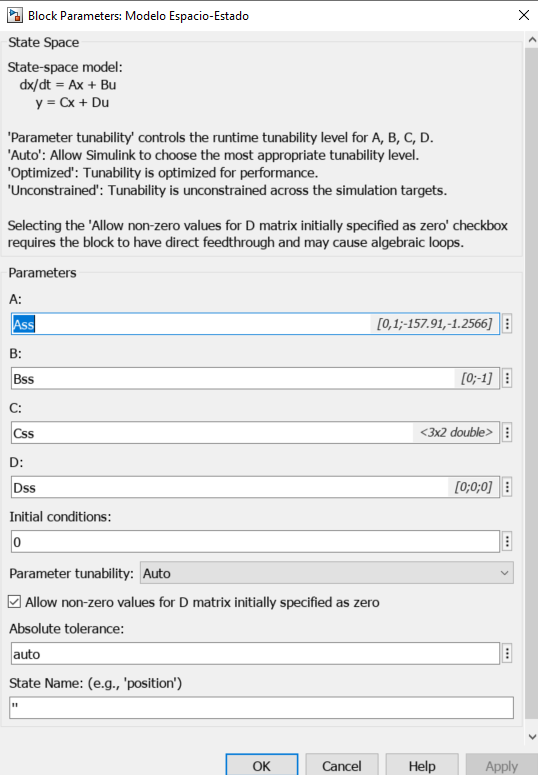
\includegraphics[width=0.5\textwidth]{Figuras/espacio estado ejemplo.png}
    \caption{Parámetros Espacio Estado ejemplo.}
    \label{fig:simulink-ss-ejemplo}
\end{figure}

\begin{figure}[H]
    \centering
    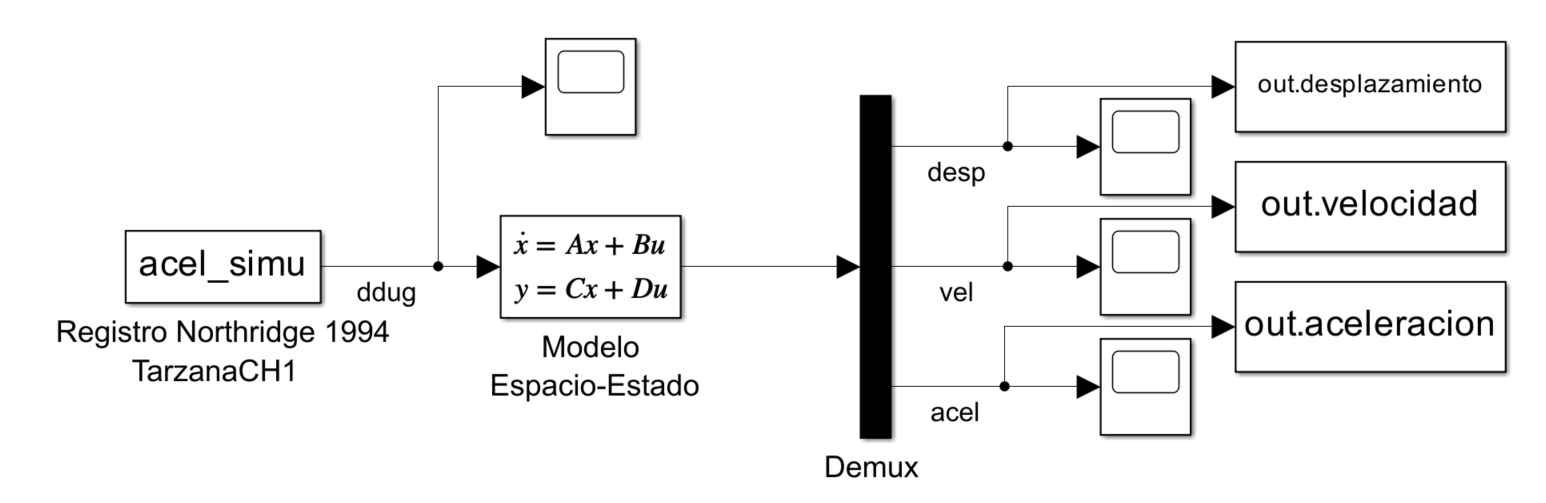
\includegraphics[width=1\textwidth]{Figuras/modelo simulink ejemplo.png}
    \caption{Modelo Simulink ejemplo.}
    \label{fig:simulink-ejemplo}
\end{figure}

Aparte se incorporan bloques \textbf{scope} en todas las señales para poder observarlas antes de llevar los datos al espacio de trabajo.

Finalmente, para llamar las variables desde el espacio de trabajo y correr la simulación se utiliza el siguiente código.

\begin{verbatimg}
%% Cargar el modelo de Simulink

modelo = 'ejemplo_Dinav'; % Nombre del archivo sin la extensión .slx
load_system(modelo);
% Ejecutar la simulación
simOut = sim(modelo);
% solución numerica
d = simOut.desplazamiento.Data;
v = simOut.velocidad.Data;
a = simOut.aceleracion.Data;

\end{verbatimg}

\end{document}

